\documentclass[reqno]{amsart}

% required packages
%
\usepackage[mathscr]{euscript}
\usepackage{amssymb}
\usepackage{graphicx}
\usepackage[shortlabels]{enumitem}
\usepackage{mathtools}
\usepackage{booktabs}
\usepackage[dvipsnames]{xcolor}
\usepackage{tikz}
\usepackage{tikz-3dplot}
\usetikzlibrary{decorations.pathreplacing}
\usetikzlibrary{decorations.markings}
\usetikzlibrary{positioning,cd,arrows, patterns}
\usetikzlibrary{arrows.meta}
\usepackage{pgfplots}
\pgfplotsset{compat=1.17}
\usepackage{subfigure}
\usepackage{ragged2e}
\usepackage{a4wide}
\usepackage{comment}
\usepackage{hyperref}
\hypersetup{colorlinks}
\usepackage{amsbsy}
\usepackage{xargs}
\usepackage{multirow}
\usepackage{array}
\usepackage{float}
\usepackage{colonequals}
\hypersetup{
%    bookmarks=true,         % show bookmarks bar?
%    unicode=false,          % non-Latin characters in Acrobat’s bookmarks
%    pdftoolbar=true,        % show Acrobat’s toolbar?
%    pdfmenubar=true,        % show Acrobat’s menu?
%    pdffitwindow=false,     % window fit to page when opened
%    pdfstartview={FitH},    % fits the width of the page to the window
%    pdftitle={My title},    % title
%    pdfauthor={Author},     % author
%    pdfsubject={Subject},   % subject of the document
%    pdfcreator={Creator},   % creator of the document
%    pdfproducer={Producer}, % producer of the document
%    pdfkeywords={keyword1} {key2} {key3}, % list of keywords
%    pdfnewwindow=true,      % links in new PDF window
colorlinks=true,       % false: boxed links; true: colored links
linkcolor=blue,          % color of internal links (change box color with linkbordercolor)
citecolor=red,        % color of links to bibliography
filecolor=violet,      % color of file links
urlcolor=violet       % color of external links
}
\usepackage{caption} 
\captionsetup[table]{skip=10pt}

\makeatletter
\def\paragraph{\@startsection{paragraph}{4}%
  \z@\z@{-\fontdimen2\font}%
  {\normalfont\bfseries}}
\makeatother

% Theorem-like environments

\theoremstyle{plain}
\newtheorem{theorem}{Theorem}[section]
\newtheorem{lemma}[theorem]{Lemma}
\newtheorem{proposition}[theorem]{Proposition}
\newtheorem{corollary}[theorem]{Corollary}
\newtheorem{claim}[theorem]{Claim}

\theoremstyle{remark}
\newtheorem{remark}[theorem]{Remark}
\newtheorem{question}[theorem]{Question}

\theoremstyle{definition}
\newtheorem{definition}[theorem]{Definition}
\newtheorem{assumption}[theorem]{Assumption}
\newtheorem{example}[theorem]{Example}


% Math operators
\DeclareMathOperator{\mmon}{\mu mon}
\DeclareMathOperator{\cl}{Cl}
\DeclareMathOperator{\Sh}{\mathscr{S}\mathsf{h}}
\DeclareMathOperator{\Loc}{\mathscr{L}\mathsf{oc}}

% Generic Math symbols
% blackboard bold
\newcommand\bbA{\mathbb{A}}
\newcommand\R{\mathbb{R}}
\newcommand\bbC{\mathbb{C}}
\newcommand\D{\mathbb{D}}
\newcommand\Z{\mathbb{Z}}
\newcommand\N{\mathbb{N}}
\newcommand\bS{\mathbb{S}}

% bold
\newcommand\bfa{\mathbf{a}}
\newcommand\bfb{\mathbf{b}}
\newcommand\bfc{\mathbf{c}}
\newcommand\bfd{\mathbf{d}}
\newcommand\bfe{\mathbf{e}}
\newcommand\bfs{\mathbf{s}}
\newcommand\bfx{\mathbf{x}}
\newcommand\bfy{\mathbf{y}}
\newcommand\bfz{\mathbf{z}}

% calligraphic
\newcommand\cA{\mathcal{A}}
\newcommand\cC{\mathcal{C}}
\newcommand\cF{\mathcal{F}}
\newcommand\cL{\mathcal{L}}
\newcommand\cM{\mathcal{M}}
\newcommand\cX{\mathcal{X}}

% sf font
\newcommand\sfI{\mathsf{I}}
\newcommand\sfT{\mathsf{T}}
\newcommand\sfY{\mathsf{Y}}


% paper specific math symbols

\newcommand{\clusterfont}{\mathcal}
\newcommand{\dynkinfont}{\mathsf}
\newcommand{\ngraphfont}{\mathscr}

% commands for clusters
\newcommand{\quiver}{\clusterfont{Q}}
\newcommand{\qbasis}{\clusterfont{\tilde{B}}}
\newcommand{\qbasispr}{\clusterfont{B}}
\newcommand{\qcoxeter}{\mutation_{\quiver}}
\DeclareMathOperator{\exchange}{Ex}
\DeclareMathOperator{\pr}{pr}
\newcommand{\qbpr}{\clusterfont{B}}
\newcommand{\exchangesub}[2]{\exchange({#1},{#2})}

% commands for N-graphs
\newcommand{\ngraph}{\ngraphfont{G}}
\newcommand{\nbasis}{\ngraphfont{B}}
\newcommand{\ncoxeter}{\mutation_\ngraph}
\newcommand{\coxeterpadding}{\ngraphfont{C}}
\newcommand{\nannulus}{\ngraphfont{A}}

% Dynkin diagrams
\newcommand{\dynA}{\dynkinfont{A}}
\newcommand{\dynB}{\dynkinfont{B}}
\newcommand{\dynC}{\dynkinfont{C}}
\newcommand{\dynD}{\dynkinfont{D}}
\newcommand{\dynE}{\dynkinfont{E}}
\newcommand{\dynF}{\dynkinfont{F}}
\newcommand{\dynG}{\dynkinfont{G}}
\newcommand{\dynX}{\dynkinfont{Z}}
%\newcommand{\dynY}{\dynkinfont{Y}}
\newcommand{\dynY}{{\dynkinfont{Z}^G}}

\newcommand{\dynADE}{\dynkinfont{ADE}}
\newcommand{\dynBCFG}{\dynkinfont{BCFG}}

\newcommand{\exdynA}{\widetilde{\dynA}}
\newcommand{\exdynB}{\widetilde{\dynB}}
\newcommand{\exdynC}{\widetilde{\dynC}}
\newcommand{\exdynD}{\widetilde{\dynD}}
\newcommand{\exdynE}{\widetilde{\dynE}}
\newcommand{\exdynF}{\widetilde{\dynF}}
\newcommand{\exdynG}{\widetilde{\dynG}}
\newcommand{\exdynX}{\widetilde{\dynX}}


% other symbols
\newcommand{\facet}{\mathscr{F}}
\newcommand{\seed}{\Sigma}
\newcommand{\initialseed}{\Sigma_{t_0}}
\newcommand{\flags}{\mathcal{F}_\legendrian}
\newcommand{\mutation}{\mu}
\DeclareMathOperator{\Fan}{Fan}
\DeclareMathOperator{\re}{re}

\newcommand{\annulus}{\mathbb{A}}
\newcommand{\disk}{\mathbb{D}}
\newcommand{\sphere}{\mathbb{S}}

\newcommand{\legendrian}{\lambda}
\newcommand{\Legendrian}{\Lambda}

\newcommand{\Ngraphs}{\mathscr{N}\mathsf{graphs}}

\newcommand{\boundary}{\partial}
\newcommand{\cycle}{\gamma}

\newcommand{\field}{\mathbb{F}}

\newcommand{\Roots}{\Phi}
\newcommand{\SRoots}{\Pi}
\newcommand{\alposRoots}{\Roots_{\ge -1}}

\newcommand{\Move}[1]{{\rm{(#1)}}}

\newcommand{\wavefront}{\Gamma}

\newcommand{\boundellipse}[3]% center, xdim, ydim
{(#1) ellipse (#2 and #3)}


\newcommand{\1}{\sigma_1}
\newcommand{\2}{\sigma_2}
\newcommand{\3}{\sigma_3}
\newcommand{\4}{\sigma_4}
\newcommand{\5}{\sigma_{1,3}}


\newcommand{\reducedto}{\succ}


%\newcommand{\yjnote}[1]{\marginpar{\RaggedRight\hsize1.7cm\tiny{\color{cyan}\raggedright #1}}}
%\newcommand{\ejnote}[1]{\marginpar{\RaggedRight\hsize1.7cm\tiny{\color{magenta}\raggedright #1}}}
%\newcommand{\bhnote}[1]{\marginpar{\RaggedRight\hsize1.7cm\tiny{\color{blue}\raggedright #1}}}




\colorlet{cyclecolor1}{orange}
\colorlet{cyclecolor2}{green}
\colorlet{cyclecolor3}{black}
\colorlet{cyclecolor4}{violet}
\def\cyclecolornamefirst{orange}
\def\cyclecolornamesecond{green}


%%%% Eunjeong_header_start %%%%
\numberwithin{equation}{section}
%\numberwithin{table}{section}
%%% tikzset

\tikzset{ynode/.style = {circle, fill=cyclecolor1, inner sep = 2pt, opacity = 0.5}}
\tikzset{gnode/.style = {circle, fill=cyclecolor2, inner sep = 2pt, opacity = 0.5}}
\tikzset{bnode/.style = {circle, fill=cyclecolor3, inner sep = 2pt, opacity = 0.5}}
\tikzset{vnode/.style = {circle, fill=cyclecolor4, inner sep = 2pt, opacity = 0.5}}
\tikzstyle{Dnode}=[draw, circle, inner sep = 0.07cm]
\tikzstyle{double line} = [
decoration={
    markings,
    mark=at position 0.55 with {\arrow[line width = 0.5pt,scale=1]{angle 90}}},
	double distance = 1.5pt, 
	double=\pgfkeysvalueof{/tikz/commutative diagrams/background color},
	postaction={decorate}
]


\tikzstyle{triple line} = [
decoration={
    markings,
    mark=at position 0.55 with {\arrow[line width = 0.5pt,scale=1]{angle 90}}},
	double distance = 2pt, 
	double=\pgfkeysvalueof{/tikz/commutative diagrams/background color},
	postaction={decorate}
]

\tikzset{Dble/.style args={#1 and #2}{%
decoration={%
markings,% switch on markings
mark=at position 0 with {%
    \coordinate (Axx) at (0,.5\pgflinewidth);%
    \coordinate (Bxx) at (0,-.5\pgflinewidth);},%
mark=at position 1 with {%
    \coordinate (Ayy) at (0,.5\pgflinewidth);%
    \coordinate (Byy) at (0,-.5\pgflinewidth);%
    \draw [#1] (Axx)--(Ayy) ;%
    \draw [#2] (Bxx)--(Byy) ;}%
},%
postaction={decorate}}
}

\tikzset{
  % style to apply some styles to each segment of a path
  on each segment/.style={
    decorate,
    decoration={
      show path construction,
      moveto code={},
      lineto code={
        \path [#1]
        (\tikzinputsegmentfirst) -- (\tikzinputsegmentlast);
      },
      curveto code={
        \path [#1] (\tikzinputsegmentfirst)
        .. controls
        (\tikzinputsegmentsupporta) and (\tikzinputsegmentsupportb)
        ..
        (\tikzinputsegmentlast);
      },
      closepath code={
        \path [#1]
        (\tikzinputsegmentfirst) -- (\tikzinputsegmentlast);
      },
    },
  },
  % style to add an arrow in the middle of a path
  mid arrow/.style={postaction={decorate,decoration={
        markings,
        mark=at position .5 with {\arrow[#1]{stealth}}
      }}},
} 
%%%% Eunjeong_header_end %%%%


%% circled 
%\newcommand*\circled[1]{\tikz[baseline=(char.base)]{
%            \node[violet,shape=circle,draw,inner sep=0pt] (char) {#1};}}
\newcommand*\circled[1]{\tikz[baseline=(char.base)]{
\node[shape=circle,draw,inner sep=0.8pt] (char) {#1};}}



% BH's pgfkey for curly brace
\makeatletter 
\tikzset{curlybrace/.style={rounded corners=2pt,line cap=round}}%  
\pgfkeys{% https://tex.stackexchange.com/a/45129/121799
/curlybrace/.cd,%
tip angle/.code     =  \def\cb@angle{#1},
/curlybrace/.unknown/.code ={\let\searchname=\pgfkeyscurrentname
                          \pgfkeysalso{\searchname/.try=#1,
                          /tikz/\searchname/.retry=#1}}}  
\def\curlybrace{\pgfutil@ifnextchar[{\curly@brace}{\curly@brace[]}}%

\def\curly@brace[#1]#2#3#4{% 
\pgfkeys{/curlybrace/.cd,
tip angle = 0.75}% 
\pgfqkeys{/curlybrace}{#1}% 
\ifnum 1>#4 \def\cbrd{0.05} \else \def\cbrd{0.075} \fi
\draw[/curlybrace/.cd,curlybrace,#1]  (#2:#4-\cbrd) -- (#2:#4) arc (#2:{(#2+#3)/2-\cb@angle}:#4) --({(#2+#3)/2}:#4+\cbrd) coordinate (curlybracetipn);
\draw[/curlybrace/.cd,curlybrace,#1] ({(#2+#3)/2}:#4+\cbrd) -- ({(#2+#3)/2+\cb@angle}:#4) arc ({(#2+#3)/2+\cb@angle} :#3:#4) --(#3:#4-\cbrd);
}
\makeatother


% paper title
\title{Lagrangian fillings for Legendrian links of finite or affine Dynkin type}

\author{Byung Hee An}
\email{anbyhee@knu.ac.kr}
\address{Department of Mathematics Education, Kyungpook National University, Republic of Korea}

\author{Youngjin Bae}
\email{yjbae@inu.ac.kr}
\address{Department of Mathematics, Incheon National University, Republic of Korea}

\author{Eunjeong Lee}
\email{eunjeong.lee@ibs.re.kr}
\address{Center for Geometry and Physics, Institute for Basic Science (IBS), Pohang 37673, Republic of Korea}
\keywords{Legendrian link, Lagrangian filling, Cluster algebra}
\subjclass[2010]{Primary: 53D10, 13F60. Secondary: 57R17.}

\begin{document}

\begin{abstract}
We prove that there are at least as many exact embedded Lagrangian fillings 
as seeds for Legendrian links of finite type $\dynADE$ or affine type $\exdynD \exdynE$. We also provide 
as many Lagrangian fillings with rotational symmetry as seeds of type $\dynB$, $\dynG_2$, $\exdynG_2$, $\exdynB$, or $\exdynC_2$, and with conjugation symmetry as seeds of type $\dynF_4$, $\dynC$, $\dynE_6^{(2)}$, $\exdynF_4$, or $\dynA_5^{(2)}$.
These families are the first known Legendrian links with (infinitely many) exact Lagrangian fillings (with symmetry) that exhaust all seeds in the corresponding cluster structures beyond type $\dynA \dynD$.
Furthermore, we show that the $N$-graph realization of (twice of) Coxeter mutation of type $\exdynD\exdynE$ corresponds to a Legendrian loop of the corresponding Legendrian links. Especially, the loop of type $\exdynD$ coincides with the one considered by Casals and Ng.
\end{abstract}

\maketitle

\tableofcontents

\section{Introduction}
\subsection{Background}
Legendrian knots are central objects in the study of 3-dimensional
contact manifolds. Classification of Legendrian knots is important in its
own right and also plays a prominent role in classifying 4-dimensional
Weinstein manifolds.

Classical Legendrian knot invariants are Thurston--Bennequin number and rotation
number~\cite{Gei2008} which distinguish the pair of Legendrian knots with the
same knot type. There are non-classical invariants including the Legendrian
contact algebra via the method of Floer theory~\cite{EGH2000, Che2002}, and
the space of constructible sheaves using microlocal
analysis~\cite{GKS2012,STZ2017}. These non-classical invariants distinguish
the Chekanov pair, a pair of Legendrian knots of type $m5_2$ having the same
classical invariants.


Recently, the study of exact Lagrangian fillings for Legendrian links has
been extremely plentiful. In the context of Legendrian contact algebra, an exact
Lagrangian filling gives an augmentation through the functorial view 
point~\cite{EHK2016}. There are several level of equivalence between 
augmentations
and the constructible sheaves for Legendrian links from counting to
categorical equivalence~\cite{NRSSZ2015}. 
Using these idea of
augmentations and constructible sheaves, people construct infinitely many fillings for certain Legendrian links~\cite{CG2020, GSW2020b,
CZ2020}. Here is the summarized list of methods of constructing Lagrangian
fillings for Legendrian links:
\begin{enumerate}
\item Decomposable Lagrangian fillings via pinching sequences and Legendrian loops \cite{EHK2016, Kal2006, CN2021}.
\item Alternating Legendrians and its conjugate Lagrangian fillings
\cite{STWZ2019}. 
\item Legendrian weaves via $N$-graphs and Legendrian mutations \cite{TZ2018, CZ2020}. 
\item Donaldson--Thomas transformation on augmentation varieties
\cite{SW2019, GSW2020a, GSW2020b}.
\end{enumerate}


Cluster algebras, introduced by Fomin and Zelevinsky~\cite{FZ1_2002}, play a crucial role in
the above constructions and applications. More precisely, the space of
augmentations and the moduli of constructible sheaves of microlocal rank one adapted to
Legendrian links admit structures of cluster pattern and $Y$-pattern, respectively~\cite{STWZ2019, SW2019, GSW2020a}. 
Note that a $Y$-seed of cluster algebra consists of a quiver whose vertices are
decorated with variables, called \emph{coefficients}. An involutory operation at each vertex,
called \emph{mutation}, generates all seeds of the $Y$-pattern.
The main point is to identify the
mutation in the $Y$-pattern and an operation in the space of Lagrangian
fillings. This geometric operation is deeply related to the Lagrangian surgery~\cite{Pol1991} and
the wall-crossing phenomenon~\cite{Aur2007}.


Indeed, a Legendrian torus link of type $(2,n)$ admits as many exact
Lagrangian fillings as Catalan number up to exact Lagrangian isotopy \cite{Pan2017, STWZ2019,
TZ2018}. Interestingly enough, the Catalan number is the number of seeds in a
cluster pattern of Dynkin type $\dynA_{n-1}$. 
There are also Legendrian links corresponding to finite Dynkin type $\dynD\dynE$, and affine Dynkin type $\exdynD\exdynE$ \cite{GSW2020b}.
A conjecture by Casals \cite[Conjecture~5.1]{Cas2020} says that the number of
distinct exact embedded Lagrangian fillings (up to exact Lagrangian isotopy) for
Legendrian links of type $\dynADE$ is exactly the same as the number of seeds
of the corresponding cluster algebras.

Furthermore, it is also conjectured by Casals \cite[Conjecture~5.4]{Cas2020} that for Legendrian links of type $\dynA_{2n-1}, \dynD_{n+1}, \dynE_6$ and $\dynD_4$, Lagrangian fillings having certain $\Z/2\Z$ or $\Z/3\Z$-symmetry form the cluster patterns of type $\dynB_n, \dynC_n, \dynF_4$ and $\dynG_2$, which are Dynkin diagrams obtained by \emph{folding} as explained in~\cite{FZ_Ysystem03}.


\subsection{The results}
\subsubsection{Lagrangian fillings for Legendrians of type $\dynADE$ or $\exdynD\exdynE$}
Our main result is that there are at least as many Lagrangian fillings for
Legendrian links of finite type as seeds in the corresponding cluster structures. We deal with $N$-graphs introduced by Casals and Zaslow \cite{CZ2020} to
construct the Lagrangian fillings. An $N$-graph $\ngraph$ on $\disk^2$ gives
a Legendrian surface $\Legendrian(\ngraph)$ in $J^1\disk^2$ while the
boundary $\boundary \ngraph$ on $\sphere^1$ induces a Legendrian link~$\legendrian(\boundary \ngraph)$. Then projection of $\Legendrian(\ngraph)$
along the Reeb direction becomes a Lagrangian filling of~$\legendrian(\boundary \ngraph)$.

As mentioned above, we interpret an $N$-graph as a $Y$-seed in the corresponding
$Y$-pattern. A one-cycle in the Legendrian surface
$\Legendrian(\ngraph)$ corresponds to a vertex of the quiver, and a signed
intersection between one-cycles gives an arrow between corresponding
vertices. From constructible sheaves adapted to $\Legendrian(\ngraph)$, one
can assign a monodromy to each one-cycle which becomes the coefficient at each vertex.

There is an operation so called a \emph{Legendrian mutation}
$\mutation_\cycle$ on an $N$-graph $\ngraph$ along one-cycle $[\cycle]\in
H_1(\Legendrian(\ngraph))$ which is the counterpart of the mutation on the
$Y$-pattern, see Proposition~\ref{proposition:equivariance of mutations}. The
delicate and challenging part is that we do not know whether Legendrian
mutations are always possible or not. Simply put, this is because the
mutation in cluster side is algebraic, whereas the Legendrian mutation is
rather geometric.

The main idea of our construction is to consider $N$-graphs $\ngraph(a,b,c)$ and $\ngraph(\exdynD_n)$ bounding Legendrian links $\legendrian(a,b,c)$ and $\legendrian(\exdynD_n)$, respectively.

\begin{align*}
\legendrian(a,b,c)=
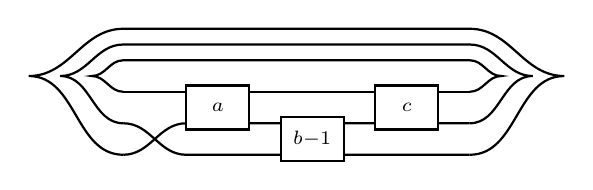
\begin{tikzpicture}[baseline=5ex,scale=0.8]
\draw[thick] (0,0) to[out=0,in=180] (1,0.5) (2,0.5) to (2.5,0.5) (3.5,0.5) to (4,0.5) (5,0.5) to (5.5,0.5);
\draw[thick] (0,0.5) to[out=0,in=180] (1,0) to (2.5,0) (3.5,0) to (5.5,0);
\draw[thick] (0,1) to[out=0,in=180] (1,1) (2,1) to (4,1) (5,1) to (5.5,1);
\draw[thick] (1,0.4) rectangle node {$\scriptstyle a$} (2, 1.1);
\draw[thick] (2.5,-0.1) rectangle node {$\scriptstyle{b-1}$} (3.5, 0.6);
\draw[thick] (4,0.4) rectangle node {$\scriptstyle c$} (5, 1.1);
\draw[thick] (0,1) to[out=180, in=0] (-0.5,1.25) to[out=0,in=180] (0,1.5) to (5.5,1.5) to[out=0,in=180] (6,1.25) to[out=180,in=0] (5.5,1);
\draw[thick] (0,0.5) to[out=180, in=0] (-1,1.25) to[out=0,in=180] (0,1.75) to (5.5,1.75) to[out=0,in=180] (6.5,1.25) to[out=180,in=0] (5.5,0.5);
\draw[thick] (0,0) to[out=180, in=0] (-1.5,1.25) to[out=0,in=180] (0,2) to (5.5,2) to[out=0,in=180] (7,1.25) to[out=180,in=0] (5.5,0);
\end{tikzpicture}
\end{align*}

\begin{align*}
\legendrian({{\exdynD}_n})=
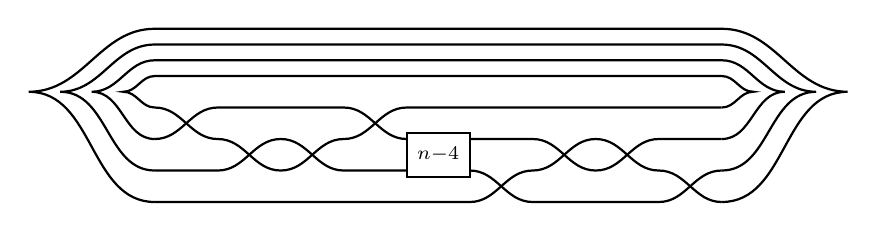
\begin{tikzpicture}[baseline=-0.5ex,scale=0.8]
%braidpart
\draw[thick] (0,0) to[out=0,in=180] (1,-0.5) to[out=0,in=180] (2,-1) to[out=0,in=180] (3,-0.5) to[out=0,in=180] (4,0) to[out=0,in=180] (9,0);
\draw[thick] (0,-0.5) to[out=0,in=180] (1,0) to[out=0,in=180] (3,0) to[out=0,in=180] (4,-0.5) (5,-0.5) to[out=0,in=180] (6,-0.5) to[out=0,in=180] (7,-1) to[out=0,in=180] (8,-0.5) to[out=0,in=180] (9,-0.5);
\draw[thick] (0,-1) to[out=0,in=180] (1,-1) to[out=0,in=180] (2,-0.5) to[out=0,in=180] (3,-1) to[out=0,in=180] (4,-1) (5,-1) to[out=0,in=180] (6,-1.5) to[out=0,in=180] (8,-1.5) to[out=0,in=180] (9,-1);
\draw[thick] (0,-1.5) to[out=0,in=180] (5,-1.5) to[out=0,in=180] (6,-1) to[out=0,in=180] (7,-0.5) to[out=0,in=180] (8,-1) to[out=0,in=180] (9,-1.5);
\draw[thick] (4,-0.4) rectangle node {$\scriptstyle{n-4}$} (5, -1.1);
%closure part
\draw[thick] (0,0) to[out=180,in=0] (-0.5,0.25) to[out=0,in=180] (0,0.5) to[out=0,in=180] (9,0.5) to[out=0,in=180] (9.5,0.25) to[out=180,in=0] (9,0);
\draw[thick] (0,-0.5) to[out=180,in=0] (-1,0.25) to[out=0,in=180] (0,0.75) to[out=0,in=180] (9,0.75) to[out=0,in=180] (10,0.25) to[out=180,in=0] (9,-0.5);
\draw[thick] (0,-1) to[out=180,in=0] (-1.5,0.25) to[out=0,in=180] (0,1) to[out=0,in=180] (9,1) to[out=0,in=180] (10.5,0.25) to[out=180,in=0] (9,-1);
\draw[thick] (0,-1.5) to[out=180,in=0] (-2,0.25) to[out=0,in=180] (0,1.25) to[out=0,in=180] (9,1.25) to[out=0,in=180] (11,0.25) to[out=180,in=0] (9,-1.5);
\end{tikzpicture}
\end{align*}
Note that the above Legendrians $\legendrian(a,b,c)$ and $\legendrian(\exdynD_n)$ can be obtained by ($-1$)-closure of the following braids, respectively,
\begin{align*}
\beta(a,b,c)&=\sigma_2\sigma_1^{a+1}\sigma_2\sigma_1^{b+1}\sigma_2\sigma_1^{c+1},&
\beta(\exdynD_n)&=\left(\sigma_2\sigma_1^3\sigma_2\sigma_1^3\sigma_2\sigma_1^k\sigma_3\right)\cdot\left(\sigma_2\sigma_1^3\sigma_2\sigma_1^3\sigma_2\sigma_1^\ell\sigma_3\right),
\end{align*}
where $k=\lfloor \frac{n-3}2\rfloor$ and $\ell=\lfloor \frac{n-4}2\rfloor$, see Section~\ref{sec:N-graph of finite or affine type}.
Those braids provide boundary data of the following $N$-graphs which represent exact Lagrangian fillings of corresponding Legendrian links:

\begin{figure}[ht]
\subfigure[$(\ngraph(a,b,c),\nbasis(a,b,c))$\label{N-graph(a,b,c)}]{
$
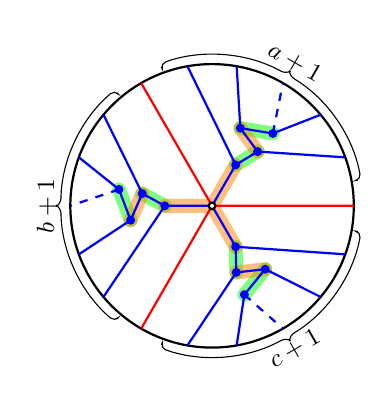
\begin{tikzpicture}[baseline=-.5ex,scale=0.6]
\draw[thick] (0,0) circle (3cm);
%\draw[line cap=round, line width=5, opacity=0.5] (3,0) -- (-1,0) (60:1) -- (100:3);
\draw[color=cyclecolor2, line cap=round, line width=5, opacity=0.5] (60:1) -- (50:1.5) (70:1.75) -- (50:2) (180:1) -- (170:1.5) (190:1.75) -- (170:2) (300:1) -- (290:1.5) (310:1.75) -- (290:2);
\draw[color=cyclecolor1, line cap=round, line width=5, opacity=0.5] (0,0) -- (60:1) (0,0) -- (180:1) (0,0) -- (300:1) (50:1.5) -- (70:1.75) (170:1.5) -- (190:1.75) (290:1.5) -- (310:1.75);
\draw[red, thick] (0,0) -- (0:3) (0,0) -- (120:3) (0,0) -- (240:3);
\draw[blue, thick, fill] (0,0) -- (60:1) circle (2pt) -- (100:3) (60:1) -- (50:1.5) circle (2pt) -- (20:3) (50:1.5) -- (70:1.75) circle (2pt) -- (80:3) (70:1.75) -- (50:2) circle (2pt) -- (40:3);
\draw[blue, thick, dashed] (50:2) -- (60:3);
\draw[blue, thick, fill] (0,0) -- (180:1) circle (2pt) -- (220:3) (180:1) -- (170:1.5) circle (2pt) -- (140:3) (170:1.5) -- (190:1.75) circle (2pt) -- (200:3) (190:1.75) -- (170:2) circle (2pt) -- (160:3);
\draw[blue, thick, dashed] (170:2) -- (180:3);
\draw[blue, thick, fill] (0,0) -- (300:1) circle (2pt) -- (340:3) (300:1) -- (290:1.5) circle (2pt) -- (260:3) (290:1.5) -- (310:1.75) circle (2pt) -- (320:3) (310:1.75) -- (290:2) circle (2pt) -- (280:3);
\draw[blue, thick, dashed] (290:2) -- (300:3);
\draw[thick, fill=white] (0,0) circle (2pt);
\curlybrace[]{10}{110}{3.2};
\draw (300:3.5) node[rotate=30] {\small ${c+1}$};
\curlybrace[]{130}{230}{3.2};
\draw (180:3.5) node[rotate=90] {\small $b+1$};
\curlybrace[]{250}{350}{3.2};
\draw (60:3.5) node[rotate=-30] {\small $a+1$};
\end{tikzpicture}
$}
\qquad
\subfigure[$(\ngraph(\exdynD_{n}),\nbasis(\exdynD_{n}))$\label{N-graph(Dn)}]{
$
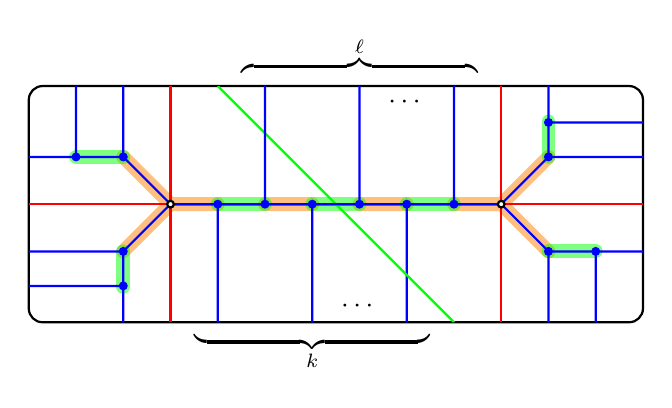
\begin{tikzpicture}[baseline=-.5ex,scale=0.6]
\draw[rounded corners=5, thick] (-6.5, -2.5) rectangle (6.5, 2.5);
\draw (0.5, -2.5) node[above] {$\cdots$} 
(-0.5, -2.5) node[below] {$\underbrace{\hphantom{\hspace{3cm}}}_{k}$};
\draw (1.5, 2.5) node[below] {$\cdots$} 
(0.5, 2.5) node[above] {$\overbrace{\hphantom{\hspace{3cm}}}^{\ell}$};
\clip[rounded corners=5] (-6.5, -2.5) rectangle (6.5, 2.5);
\draw[cyclecolor1, opacity=0.5, line cap=round, line width=5] 
(-3.5, 0) -- (-2.5, 0) (-3.5, 0) -- (-4.5, 1) (-3.5, 0) -- (-4.5, -1)
(-1.5, 0) -- (-0.5, 0)
(0.5, 0) -- (1.5, 0)
(3.5, 0) -- (2.5, 0) (3.5, 0) -- (4.5, 1) (3.5, 0) -- (4.5, -1)
;
\draw[cyclecolor2, opacity=0.5, line cap=round, line width=5] 
(-4.5, 1) -- (-5.5, 1)
(-4.5, -1) -- (-4.5, -1.75)
(-1.5, 0) -- (-2.5, 0)
(-0.5, 0) -- (0.5, 0)
(1.5, 0) -- (2.5, 0)
(4.5, 1) -- (4.5, 1.75)
(4.5, -1) -- (5.5, -1)
;
\foreach \i in {0, 180} {
\begin{scope}[rotate=\i]
\draw[thick, green] (-2.5, 2.5) -- (0,0);
\draw[thick, red] 
(-3.5, -2.5) -- (-3.5, 2.5)
(-6.5, 0) -- (-3.5, 0)
;
\draw[thick, blue, fill]
(-2.5, -2.5) -- (-2.5,0) circle (2pt)
(-0.5, -2.5) -- (-0.5,0) circle (2pt)
(1.5, -2.5) -- (1.5,0) circle (2pt)
;
\draw[thick, blue, fill] 
%
(-3.5, 0) -- (3.5, 0)
(-3.5, 0) -- (-4.5, 1) circle (2pt) -- (-4.5, 2.5)
(-4.5, 1) -- (-6.5, 1)
(-5.5, 1) circle (2pt) -- (-5.5, 2.5)
%
(-3.5, 0) -- (-4.5, -1) circle (2pt) -- (-4.5, -2.5)
(-4.5, -1) -- (-6.5, -1)
(-4.5, -1.73) circle (2pt) -- (-6.5, -1.73)
;
\end{scope}
}
\draw[thick, fill=white] (-3.5, 0) circle (2pt) (3.5, 0) circle (2pt);
\end{tikzpicture}
$}
\caption{Pairs of $N$-graphs and tuples of cycles}
\label{fig:N-graphs of (a,b,c) and Dn}
\end{figure}

\noindent Here, the \colorbox{cyclecolor1!50!}{\cyclecolornamefirst}- and \colorbox{cyclecolor2!50!}{\cyclecolornamesecond}-shaded edges indicate a tuple of one-cycles $\nbasis$ in the corresponding Legendrian surface.
See~\S\ref{sec:1-cycles in Legendrian weaves} for the detail.



The Legendrians $\legendrian(a,b,c), \legendrian(\exdynD_n)$ are the rainbow closure of \emph{positive braids}. 
By the work of Shen--Weng \cite{SW2019}, it is direct to check that 
the corresponding cluster structure of Legendrian $\legendrian(\dynX)$ is 
indeed of type $\dynX$ for $\dynX\in\{\dynA,\dynD,\dynE,\exdynD,\exdynE\}$. More precisely, the coordinate 
ring of the moduli space $\cM_1(\legendrian(\dynX))$ of microlocal rank one 
sheaves in $\Sh^\bullet_{\legendrian(\dynX)}(\R^2)$ admits the aforementioned 
$Y$-pattern structure.
By the way, the (candidate) Legendrians of type $\exdynA$ are not the rainbow 
closure of positive braids, in general. 
Indeed, Casals--Ng~\cite{CN2021} considered a Legendrian link of type 
$\exdynA_{1,1}$ which is not the rainbow closure of a  positive braid. 
So we can not directly apply the subsequent argument to Legendrians of type 
$\exdynA$.

To prove the realizability of each $Y$-seed in the corresponding $Y$-pattern, we use an induction argument on the rank of the type $\dynX$. 
More precisely, for each $Y$-pattern, we consider the \emph{exchange graph}, whose vertices are the $Y$-seeds and whose edges connect the vertices related by a single mutation. 
It has been known that the exchange graph of a $Y$-pattern is determined by the Dynkin type $\dynX$ of the $Y$-pattern when $\dynX$ is finite or affine (cf. Propositions~\ref{thm_exchange_graph_Dynkin} and~\ref{prop_Y-pattern_exchange_graph}). Because of this, we denote by $\exchange(\Roots(\dynX))$ the exchange graph of a $Y$-pattern of type $\dynX$.
Here, $\Roots(\dynX)$ is the root system of type $\dynX$. Note that when $\dynX$ is of finite type, the exchange graph $\exchange(\Roots(\dynX))$ becomes the one-skeleton of a polytope, called the (\emph{generalized}) \emph{associahedron} (see Figures~\ref{fig_asso_A3_intro} and~\ref{fig_asso_D4}).
\begin{figure}[ht]
% \todo{Draw A3 associahedron}
\tdplotsetmaincoords{110}{-30}
\begin{tikzpicture}%
[tdplot_main_coords,
% 	x={(0.497546cm, 0.859773cm)},
% y={(-0.106336cm, -0.071189cm)},
% z={(0.860895cm, -0.505690cm)},
%scale= 2,
% [x={(-0.495892cm, -0.532283cm)},
% y={(0.868384cm, -0.303848cm)},
% z={(-0.000125cm, 0.790159cm)},
scale=0.700000,
back/.style={loosely dotted, thin},
edge/.style={color=black, thick},
facet/.style={fill=blue!95!black,fill opacity=0.100000},
vertex/.style={inner sep=1pt,circle,fill=black,thick,anchor=base},
gvertex/.style={inner sep=1.2pt,circle,draw=green!25!black,fill=green!75!black,thick,anchor=base}]
%% Coordinate of the vertices:
%%
\coordinate (1) at (-0.50000, -1.50000, 2.00000);
\coordinate (2) at (1.50000, 1.50000, -2.00000);
\coordinate (3) at (0.50000, 0.50000, 1.00000);
\coordinate (4) at (0.50000, 1.50000, 0.00000);
\coordinate (5) at (1.50000, 1.50000, -1.00000);
\coordinate (6) at (-0.50000, -0.50000, 2.00000);
\coordinate (7) at (1.50000, 0.50000, 0.00000);
\coordinate (8) at (1.50000, -1.50000, 0.00000);
\coordinate (9) at (1.50000, -1.50000, -2.00000);
\coordinate (10) at (-1.50000, -1.50000, -2.00000);
\coordinate (11) at (-1.50000, -1.50000, 2.00000);
\coordinate (12) at (-1.50000, 1.50000, -2.00000);
\coordinate (13) at (-1.50000, 1.50000, 0.00000);
\coordinate (14) at (-1.50000, -0.50000, 2.00000);

%% fill some facets
\fill[cyclecolor1, opacity = 0.3] (10)--(12)--(13)--(14)--(11)--cycle;
\fill[cyclecolor2, opacity = 0.2] (10)--(9)--(8)--(1)--(11)--cycle;
\fill[yellow, opacity = 0.3] (10)--(9)--(2)--(12)--cycle;

%%
%%
%% Drawing edges in the back
%%
\draw[edge,back] (9) -- (10);
\draw[edge,back] (10) -- (11);
\draw[edge,back] (10) -- (12);
%%
%%
%% Drawing vertices in the back
%%
\node[vertex] at (10)     {};

% %%
%%
%% Drawing edges in the front
%%
\draw[edge] (1) -- (6);
\draw[edge] (1) -- (8);
\draw[edge] (1) -- (11);
\draw[edge] (2) -- (5);
\draw[edge] (2) -- (9);
\draw[edge] (2) -- (12);
\draw[edge] (3) -- (4);
\draw[edge] (3) -- (6);
\draw[edge] (3) -- (7);
\draw[edge] (4) -- (5);
\draw[edge] (4) -- (13);
\draw[edge] (5) -- (7);
\draw[edge] (6) -- (14);
\draw[edge] (7) -- (8);
\draw[edge] (8) -- (9);
\draw[edge] (11) -- (14);
\draw[edge] (12) -- (13);
\draw[edge] (13) -- (14);
%%
%%
%% Drawing the vertices in the front
%%
\node[vertex] at (1)     {};
\node[vertex] at (2)     {};
\node[vertex] at (3)     {};
\node[vertex] at (4)     {};
\node[vertex] at (5)     {};
\node[vertex] at (6)     {};
\node[vertex] at (7)     {};
\node[vertex] at (8)     {};
\node[vertex] at (9)     {};
\node[vertex] at (11)     {};
\node[vertex] at (12)     {};
\node[vertex] at (13)     {};
\node[vertex] at (14)     {};

\foreach \g in {10, 6, 5} {
\node[gvertex] at (\g) {};
}
%%
%%
%
%\foreach \x in {1,...,14}{
%\node at (\x) {\x};
%}

\end{tikzpicture}%
\hspace{1cm}%
%%
\begin{tikzpicture}%
[tdplot_main_coords,
% 	x={(0.497546cm, 0.859773cm)},
% y={(-0.106336cm, -0.071189cm)},
% z={(0.860895cm, -0.505690cm)},
%scale= 2,
% [x={(-0.495892cm, -0.532283cm)},
% y={(0.868384cm, -0.303848cm)},
% z={(-0.000125cm, 0.790159cm)},
scale=0.700000,
back/.style={loosely dotted, thin},
edge/.style={color=black, thick},
facet/.style={fill=blue!95!black,fill opacity=0.100000},
vertex/.style={inner sep=1pt,circle,fill=black,thick,anchor=base},
gvertex/.style={inner sep=1.2pt,circle,draw=green!25!black,fill=green!75!black,thick,anchor=base}]
%% Coordinate of the vertices:
%%
\coordinate (1) at (-0.50000, -1.50000, 2.00000);
\coordinate (2) at (1.50000, 1.50000, -2.00000);
\coordinate (3) at (0.50000, 0.50000, 1.00000);
\coordinate (4) at (0.50000, 1.50000, 0.00000);
\coordinate (5) at (1.50000, 1.50000, -1.00000);
\coordinate (6) at (-0.50000, -0.50000, 2.00000);
\coordinate (7) at (1.50000, 0.50000, 0.00000);
\coordinate (8) at (1.50000, -1.50000, 0.00000);
\coordinate (9) at (1.50000, -1.50000, -2.00000);
\coordinate (10) at (-1.50000, -1.50000, -2.00000);
\coordinate (11) at (-1.50000, -1.50000, 2.00000);
\coordinate (12) at (-1.50000, 1.50000, -2.00000);
\coordinate (13) at (-1.50000, 1.50000, 0.00000);
\coordinate (14) at (-1.50000, -0.50000, 2.00000);

%% fill some facets
\fill[cyclecolor1, opacity = 0.3] (6)--(3)--(7)--(8)--(1)--cycle;
\fill[cyclecolor2, opacity = 0.2] (6)--(3)--(4)--(13)--(14)--cycle;
\fill[yellow, opacity = 0.3] (6)--(1)--(11)--(14)--cycle;

%%
%%
%% Drawing edges in the back
%%
\draw[edge,back] (9) -- (10);
\draw[edge,back] (10) -- (11);
\draw[edge,back] (10) -- (12);
%%
%%
%% Drawing vertices in the back
%%
\node[vertex] at (10)     {};

% %%
%%
%% Drawing edges in the front
%%
\draw[edge] (1) -- (6);
\draw[edge] (1) -- (8);
\draw[edge] (1) -- (11);
\draw[edge] (2) -- (5);
\draw[edge] (2) -- (9);
\draw[edge] (2) -- (12);
\draw[edge] (3) -- (4);
\draw[edge] (3) -- (6);
\draw[edge] (3) -- (7);
\draw[edge] (4) -- (5);
\draw[edge] (4) -- (13);
\draw[edge] (5) -- (7);
\draw[edge] (6) -- (14);
\draw[edge] (7) -- (8);
\draw[edge] (8) -- (9);
\draw[edge] (11) -- (14);
\draw[edge] (12) -- (13);
\draw[edge] (13) -- (14);
%%
%%
%% Drawing the vertices in the front
%%
\node[vertex] at (1)     {};
\node[vertex] at (2)     {};
\node[vertex] at (3)     {};
\node[vertex] at (4)     {};
\node[vertex] at (5)     {};
\node[vertex] at (6)     {};
\node[vertex] at (7)     {};
\node[vertex] at (8)     {};
\node[vertex] at (9)     {};
\node[vertex] at (11)     {};
\node[vertex] at (12)     {};
\node[vertex] at (13)     {};
\node[vertex] at (14)     {};

\foreach \g in {10, 6, 5} {
\node[gvertex] at (\g) {};
}
%%
%%

%\foreach \x in {1,...,14}{
%\node at (\x) {\x};
%}

\end{tikzpicture} %
\hspace{1cm}%
\begin{tikzpicture}%
[tdplot_main_coords,
% 	x={(0.497546cm, 0.859773cm)},
% y={(-0.106336cm, -0.071189cm)},
% z={(0.860895cm, -0.505690cm)},
%scale= 2,
% [x={(-0.495892cm, -0.532283cm)},
% y={(0.868384cm, -0.303848cm)},
% z={(-0.000125cm, 0.790159cm)},
scale=0.700000,
back/.style={loosely dotted, thin},
edge/.style={color=black, thick},
facet/.style={fill=blue!95!black,fill opacity=0.100000},
vertex/.style={inner sep=1pt,circle,fill=black,thick,anchor=base},
gvertex/.style={inner sep=1.2pt,circle,draw=green!25!black,fill=green!75!black,thick,anchor=base}]
%% Coordinate of the vertices:
%%
\coordinate (1) at (-0.50000, -1.50000, 2.00000);
\coordinate (2) at (1.50000, 1.50000, -2.00000);
\coordinate (3) at (0.50000, 0.50000, 1.00000);
\coordinate (4) at (0.50000, 1.50000, 0.00000);
\coordinate (5) at (1.50000, 1.50000, -1.00000);
\coordinate (6) at (-0.50000, -0.50000, 2.00000);
\coordinate (7) at (1.50000, 0.50000, 0.00000);
\coordinate (8) at (1.50000, -1.50000, 0.00000);
\coordinate (9) at (1.50000, -1.50000, -2.00000);
\coordinate (10) at (-1.50000, -1.50000, -2.00000);
\coordinate (11) at (-1.50000, -1.50000, 2.00000);
\coordinate (12) at (-1.50000, 1.50000, -2.00000);
\coordinate (13) at (-1.50000, 1.50000, 0.00000);
\coordinate (14) at (-1.50000, -0.50000, 2.00000);

%% fill some facets
\fill[cyclecolor1, opacity = 0.3] (4)--(5)--(2)--(12)--(13)--cycle;
\fill[cyclecolor2, opacity = 0.2] (5)--(2)--(9)--(8)--(7)--cycle;
\fill[yellow, opacity = 0.3] (3)--(4)--(5)--(7)--cycle;

%%
%%
%% Drawing edges in the back
%%
\draw[edge,back] (9) -- (10);
\draw[edge,back] (10) -- (11);
\draw[edge,back] (10) -- (12);
%%
%%
%% Drawing vertices in the back
%%
\node[vertex] at (10)     {};

% %%
%%
%% Drawing edges in the front
%%
\draw[edge] (1) -- (6);
\draw[edge] (1) -- (8);
\draw[edge] (1) -- (11);
\draw[edge] (2) -- (5);
\draw[edge] (2) -- (9);
\draw[edge] (2) -- (12);
\draw[edge] (3) -- (4);
\draw[edge] (3) -- (6);
\draw[edge] (3) -- (7);
\draw[edge] (4) -- (5);
\draw[edge] (4) -- (13);
\draw[edge] (5) -- (7);
\draw[edge] (6) -- (14);
\draw[edge] (7) -- (8);
\draw[edge] (8) -- (9);
\draw[edge] (11) -- (14);
\draw[edge] (12) -- (13);
\draw[edge] (13) -- (14);
%%
%%
%% Drawing the vertices in the front
%%
\node[vertex] at (1)     {};
\node[vertex] at (2)     {};
\node[vertex] at (3)     {};
\node[vertex] at (4)     {};
\node[vertex] at (5)     {};
\node[vertex] at (6)     {};
\node[vertex] at (7)     {};
\node[vertex] at (8)     {};
\node[vertex] at (9)     {};
\node[vertex] at (11)     {};
\node[vertex] at (12)     {};
\node[vertex] at (13)     {};
\node[vertex] at (14)     {};

\foreach \g in {10, 6, 5} {
\node[gvertex] at (\g) {};
}
%%
%%
%
%\foreach \x in {1,...,14}{
%\node at (\x) {\x};
%}

\end{tikzpicture}
\caption{The type $\dynA_3$ associahedron}\label{fig_asso_A3_intro}
\end{figure}

A (fixed) sequence of mutations corresponding to a chosen Coxeter element provides an action on the exchange graph. We call this specific sequence of mutations a \emph{Coxeter mutation} $\mutation_{\quiver}$. The orbit of the initial seed is called \emph{bipartite belt}. The green dots in Figure~\ref{fig_asso_A3_intro} present the elements of the bipartite belt.
We notice that the facets meeting at the initial seed correspond to the exchange graphs $\exchange(\Roots(\dynX\setminus \{i\}))$. In Figure~\ref{fig_asso_A3_intro}, there are two pentagons and one square intersecting a green dot. Indeed, a pentagon is the type $\dynA_2$ generalized associahedron; a square is the type $\dynA_1 \times \dynA_1$ generalized associahedron. Moreover, by applying the Coxeter mutation on these facets iteratively, one can obtain all facets in the associahedron. 
Even though we do not have a polytope model for the exchange graph of affine type, similar properties hold, that is, one can reach any $Y$-seed in the exchange graph from the initial seed by taking Coxeter mutations and then applying a certain sequence of mutations omitting at least one vertex. 

The following good properties of the above pairs $(\ngraph(a,b,c),\nbasis(a,b,c))$ and $(\ngraph(\exdynD_{n}),\nbasis(\exdynD_{n}))$ play a crucial role in interpreting the Coxeter mutation $\qcoxeter$ in terms of $N$-graphs:
\begin{enumerate}
\item The geometric and algebraic intersection numbers between chosen one-cycles coincide. 
\item The corresponding quivers $\quiver(a,b,c)$, $\quiver(\exdynD_n)$ are bipartite, see~\S\ref{sec:N-graphs and seeds} for the details. 
\end{enumerate}
The property (2) naturally splits $\nbasis$ into two subsets $\nbasis_+$ and $\nbasis_-$.
In Figure~\ref{fig:N-graphs of (a,b,c) and Dn}, they consist of \colorbox{cyclecolor1!50!}{\cyclecolornamefirst}- and \colorbox{cyclecolor2!50!}{\cyclecolornamesecond}-shaded edges, respectively. 
Then the property (1) enables us to perform the \emph{Legendrian Coxeter mutation}, which is the $N$-graph realization of the Coxeter mutation defiend by the sequence of Legendrian mutations:
\[
\ncoxeter=\prod_{\cycle \in \nbasis_+} \mutation_{\cycle}\cdot\prod_{\cycle\in \nbasis_-} \mutation_{\cycle}.
\]
Then the resulting $N$-graphs $\ncoxeter(\ngraph(a,b,c),\nbasis(a,b,c))$ and $\ncoxeter(\ngraph(\exdynD_n),\nbasis(\exdynD_n))$ become the
$N$-graphs shown in Figure~\ref{figure:intro_Legendrian Coxeter mutation} up to a sequence of Move~\Move{II} in Figure~\ref{fig:move1-6}.
\begin{figure}[ht]
\subfigure[$\ncoxeter(\ngraph(a,b,c),\nbasis(a,b,c))$\label{ncoxeter_n(a,b,c)}]{
$
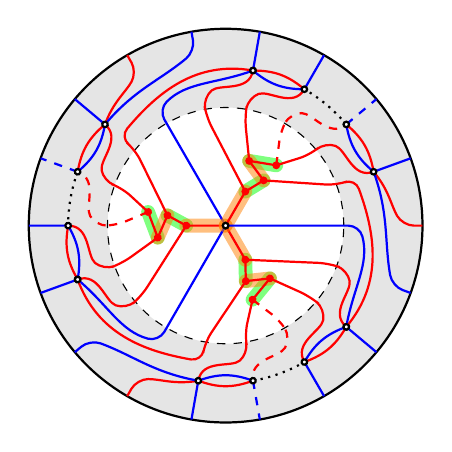
\begin{tikzpicture}[baseline=-.5ex,xscale=0.5, yscale=0.5]
\draw[thick] (0,0) circle (5cm);
\draw[dashed]  (0,0) circle (3cm);
\fill[opacity=0.1, even odd rule] (0,0) circle (3) (0,0) circle (5);
\foreach \i in {1,2,3} {
\begin{scope}[rotate=\i*120]
\draw[color=cyclecolor2, line cap=round, line width=5, opacity=0.5] (60:1) -- (50:1.5) (70:1.75) -- (50:2);
\draw[color=cyclecolor1, line cap=round, line width=5, opacity=0.5] (0,0) -- (60:1) (50:1.5) -- (70:1.75);
%
\draw[blue, thick, rounded corners] (0,0) -- (0:3.4) to[out=-75,in=80] (-40:4);
\draw[red, thick, fill] (0,0) -- (60:1) circle (2pt) (60:1) -- (50:1.5) circle (2pt) -- (70:1.75) circle (2pt) -- (50:2) circle (2pt);
\draw[red, thick, dashed, rounded corners] (50:2) -- (60:2.8) -- (60:3.3) to[out=0,in=220] (40:4);
\draw[red, thick, rounded corners] (50:2) -- (40:2.8) -- (40:3.3) to[out=-20,in=200] (20:4) (70:1.75) -- (80:2.8) -- (80:3.3) to[out=20,in=240] (60:4) (60:1) -- (100:2.8) -- (100:3.3) to[out=40,in=260] (80:4);
\draw[red, thick, rounded corners] (50:1.5) -- (20:3) -- (20:3.5) to[out=-70,in=50] (-40:4) (20:4) to[out=-50,in=120] (0:4.5) -- (0:5);
\draw[red, thick] (20:4) to[out=100,in=-40] (40:4) (60:4) to[out=140,in=0] (80:4);
\draw[blue, thick] (20:5) -- (20:4) to[out=140,in=-80] (40:4) (60:5) -- (60:4) to[out=180,in=-40] (80:4) -- (80:5);
\draw[thick, dotted] (40:4) arc (40:60:4);
\draw[blue, thick, rounded corners] (20:4) to[out=-70,in=100] (-20:4.5) -- (-20:5);
\draw[blue, thick, dashed] (40:4) -- (40:5);
\draw[fill=white, thick] (20:4) circle (2pt) (40:4) circle (2pt) (60:4) circle (2pt) (80:4) circle (2pt) (-40:4) circle (2pt);
\end{scope}
\draw[fill=white, thick] (0,0) circle (2pt);
}
\end{tikzpicture}
$}
\qquad
\subfigure[$\ncoxeter(\ngraph(\exdynD_{4}),\nbasis(\exdynD_{4}))$\label{ncoxeter_D4}]{
$
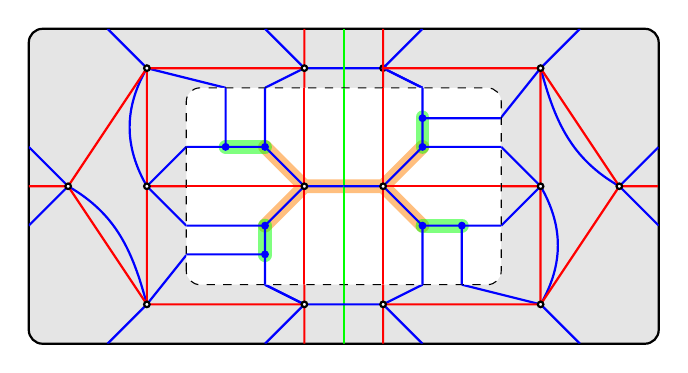
\begin{tikzpicture}[baseline=-.5ex,xscale=0.5, yscale=-0.5]
\fill[opacity=0.1, rounded corners=5] (-8, -4) rectangle (8, 4);
\draw[rounded corners=5, thick] (-8, -4) rectangle (8, 4);
\clip[rounded corners=5] (-8, -4) rectangle (8, 4);
\foreach \r in {0, 180} {
\begin{scope}[rotate=\r]
\draw[blue, thick]
(-4, 1) -- ++(-1, -1)
(-4, -1) -- ++(-1, 1) to[out=-120, in=120] ++(0,-3)
(-5, 3) to[out=-105,in=30] (-7,0)
%
(-2, -2.5) -- ++(1, -0.5) -- +(-1, -1)
++(0,0) -- ++(2, 0) -- ++(1, 0.5)
(-3, -2.5) -- ++(-2, -0.5) -- ++(-1, -1)
(-4, 1.75) -- ++(-1, 1.25) -- ++(-1, 1)
(-2, 2.5) -- ++(1, 0.5) -- ++(-1, 1)
(-8, 1) -- ++(1, -1) -- ++(-1, -1)
;
\draw[red, thick] 
(-1, -2.5) -- ++(0, -0.5) -- +(0, -1)
++(0,0) -- ++(-4, 0) -- ++(0, 3) -- +(1,0)
++(0,0) -- ++(0,3) -- ++(4,0) -- +(0, 1)
++(0,0) -- ++(0, -0.5)
(-5, -3) -- ++(-2, 3) -- +(-1, 0)
++(0,0) -- ++(2, 3)
;
\draw[green, thick] (0, 4) -- (0, 2.5);
\draw[fill=white, thick] 
(-5, 0) circle (2pt) (-7, 0) circle (2pt)
(-5, -3) circle (2pt) (-1, -3) circle (2pt) (1, -3) circle (2pt)
(-5, 3) circle (2pt)
;
\end{scope}
}
\begin{scope}[yscale=-1]
\draw[fill=white, rounded corners=5,dashed] (-4, -2.5) rectangle (4, 2.5);
\clip[rounded corners=5] (-4, -2.5) rectangle (4, 2.5);
\draw[cyclecolor1, opacity=0.5, line cap=round, line width=5]
(-1, 0) -- (1, 0) (-1, 0) -- (-2, 1) (-1, 0) -- (-2, -1)
(1, 0) -- (2, 1) (1, 0) -- (2, -1)
;
\draw[cyclecolor2, opacity=0.5, line cap=round, line width=5] 
(-2, 1) -- (-3, 1)
(-2, -1) -- (-2, -1.75)
(2, 1) -- (2, 1.75)
(2, -1) -- (3, -1)
;
\foreach \i in {0, 180} {
\begin{scope}[rotate=\i]
\begin{scope}[xshift=2.5cm]
\draw[thick, green] (-2.5, 2.5) -- ++(0,-2.5);
\draw[thick, red] 
(-3.5, -2.5) -- (-3.5, 2.5)
(-6.5, 0) -- (-3.5, 0)
;
\draw[thick, blue, fill] 
%
(-3.5, 0) -- (-2.5, 0)
(-3.5, 0) -- (-4.5, 1) circle (2pt) -- (-4.5, 2.5)
(-4.5, 1) -- (-6.5, 1)
(-5.5, 1) circle (2pt) -- (-5.5, 2.5)
%
(-3.5, 0) -- (-4.5, -1) circle (2pt) -- (-4.5, -2.5)
(-4.5, -1) -- (-6.5, -1)
(-4.5, -1.73) circle (2pt) -- (-6.5, -1.73)
;
\end{scope}
\end{scope}
}
\draw[thick, fill=white] (-1, 0) circle (2pt) (1, 0) circle (2pt);
\end{scope}
\end{tikzpicture}
$}
\caption{After applying Legendrian Coxeter mutation on the initial pair}
\label{figure:intro_Legendrian Coxeter mutation}
\end{figure}

Removing the gray-shaded annulus region, $(\ngraph(\exdynD_n),\nbasis(\exdynD_n))$ and $\ncoxeter(\ngraph(\exdynD_n),\nbasis(\exdynD_n))$ are identical, and the only difference between
$(\ngraph(a,b,c),\nbasis(a,b,c))$ and $\ncoxeter(\ngraph(a,b,c),\nbasis(a,b,c))$ is the reverse of the color. Note that the intersection pattern between one-cycles and the
Legendrian mutability are preserved under the action of the Legendrian Coxeter mutation
$\ncoxeter$.
% Moreover, the operation $\qcoxeter$ also acts on the face poset of the generalized associahedron of the root system $\Roots$.
By the induction argument on the rank of root system, we conclude that there
in no (geometric) obstruction to realize each seed via the $N$-graph.

Note that the $N$-graphs $\ngraph(a,b,c)$ and $\ngraph(\exdynD_{n})$ cover Lagrangian fillings of Legendrian links of type $\dynX\in\{\dynA,\dynD,\dynE,\exdynD,\exdynE\}$, see Table~\ref{table:short notations}.
In particular, $\ngraph(a,b,c)$ is of type $\dynADE$ or $\exdynD\exdynE$ if and only if $\frac 1a+\frac 1b+\frac 1c>1$ or $\frac 1a+\frac 1b+\frac 1c=1$, respectively.

This guarantees that there are at least as many Lagrangian fillings as seeds for $\legendrian(\dynX)$ for $\dynX\in\{\dynA,\dynD,\dynE,\exdynD,\exdynE\}$.


\begin{theorem}[Theorem~\ref{theorem:seed many fillings}]\label{thm_intro_1}
Let $\legendrian$ be a Legendrian knot or link of type~$\dynADE$ or type $\exdynD\exdynE$.
Then it admits as many exact embedded Lagrangian fillings as the number of seeds in the seed pattern of the same type.
See Table~\ref{table_seeds_and_cluster_variables} for the number of seeds of finite type. 
\end{theorem}

There are several ways of constructing exact embedded Lagrangian fillings as mentioned above.
Especially in $\dynD_4$ case, there are 34 distinct Lagrangian fillings constructed by the method of the alternating Legendrians \cite{BFFH2018,STWZ2019},
while the above $N$-graphs give seeds many 50 Lagrangian fillings.
Most recently, for Legendrian links of type $\dynD_n$, Hughes \cite{Hughes2021} makes use of $3$-graphs together with 1-cycles to show that every sequence of quiver mutations can be realized by Legendrian weave mutations. Compared with our strategy using structural results of the cluster pattern, he studies $3$-graph moves arise from quivers of type $\dynD_n$ in a more direct and concrete way. As a corollary, he also obtained at least as many Lagrangian fillings as seeds in the cluster algebra of type $\dynD_n$.

There are many results showing the existence of (infinitely many) distinct Lagrangian fillings for Legendrian links, see \cite{EHK2016,Pan2017,TZ2018,STWZ2019,CG2020,CZ2020,GSW2020b,CN2021}. To the best of authors' knowledge, Theorem~\ref{thm_intro_1} is the first results of (infinitely many) Lagrangian fillings of Legendrian links which exhaust all seeds in the corresponding cluster pattern beyond type $\dynA\dynD$.

The gray-shaded annular $N$-graphs in the above figure can be seen as exact Lagrangian cobordisms. 
In particular, the annular $N$-graph in $\ncoxeter(\ngraph(\exdynD_{4}),\nbasis(\exdynD_{4}))$ corresponds to the cobordism from the Legendrian $\legendrian(\exdynD_4)$ onto itself which defines the \emph{Legendrian loop} $\vartheta(\exdynD_4)$. 
See Figure~\ref{fig:legendrian loop of D_intro} in general.
Note that this coincides with the Legendrian loop described in \cite[Figure~2]{CN2021} up to Reidemeister moves. For type~$\exdynE$, the twice of 
Legendrian Coxeter mutation on the pair $(\ngraph(a,b,c),\nbasis(a,b,c))$ gives
the Legendrian loop~$\vartheta(\exdynE)$ of $\legendrian(\exdynE)$ as shown in Figure~\ref{fig:legendrian loop of E_intro}.
The Legendrian loop $\vartheta(\exdynE)$ can be interpreted as the move of the half twist $\Delta_3$ along the three-strand braid band, whereas the Legendrian loop $\vartheta(\exdynD_n)$ is essentially the move of the half twist $\Delta_2$ along the two-strand braid band as depicted in Figure~\ref{fig:legendrian loop of D_intro}.

\begin{figure}[ht]
\subfigure[$\coxeterpadding({\exdynD}_{n})$]{
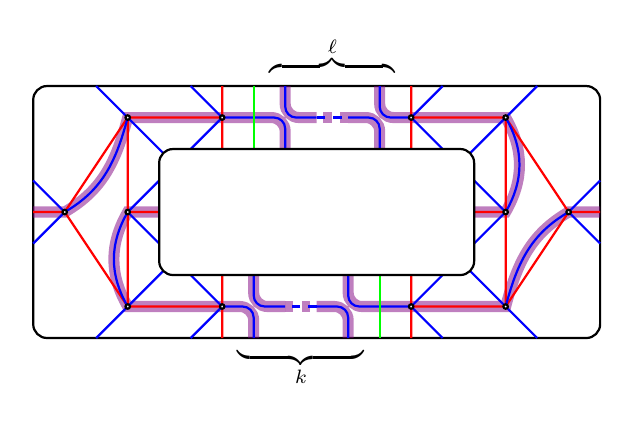
\begin{tikzpicture}[baseline=-.5ex,scale=0.4]
\draw[thick, rounded corners=5] (-9,-4) rectangle (9, 4);
\foreach \r in {0, 180} {
\begin{scope}[rotate=\r]
\begin{scope}
\draw[violet, line width=4, opacity=0.5, rounded corners=5](2,2)--(2,3)--(1,3) (0,3)--(-1,3)--(-1,4) (-1,2)--(-1,3)--(-3,3) (-3,-3)--(-2,-3)--(-2,-4);
\draw[violet, line width=4, opacity=0.5]
(-3,3)--(-6,3) to[out=-105,in=30] (-8,0) --(-9,0)
(-5,0)--(-6,0) to[out=-120,in=120] (-6,-3) -- (-3,-3);
\draw[violet, line width=4, opacity=0.5,dashed](1,3)--(0,3);
\end{scope}
\begin{scope}[yscale=-1]
\draw[thick, red]
(-3, 4) -- ++(0, -2) (-3, -4) -- ++(0, 2)
(-3, 3) -- ++(-3, 0) -- ++(0, -6) -- ++(3,0) (-6, 0) -- ++(1, 0)
(-6, 3) -- ++(-2, -3) -- ++(2, -3)
(-8, 0) -- ++(-1, 0)
;
\draw[thick, blue]
(-4, 4) -- ++(1, -1) -- ++(-1, -1) (-4, -4) -- ++(1, 1) -- ++(-1, 1)
(-7, 4) -- ++(1, -1) -- ++(1.5, -1.5) (-7, -4) -- ++(1, 1) -- ++(1.5, 1.5)
(-6, 0) -- ++(1, 1) (-6, 0) -- ++(1,-1)
(-8, 0) -- ++(-1, 1) (-8, 0) -- ++(-1, -1)
(-8, 0) to[out=-30, in=105] ++(2, -3)
(-6, 3) to[out=-120, in=120] (-6, 0)
;
\end{scope}
\draw[thick, blue, rounded corners]
(-3, 3) -- ++(2, 0) -- ++(0, -1)
(-1, 4) -- ++(0, -1) -- ++(1,0)
(2, 2) -- ++(0, 1) -- ++(-1, 0)
(-2, -4) -- ++(0, 1) -- ++(-1, 0)
;
\draw[thick, blue, dashed]
(0, 3) -- ++(1, 0)
;
\draw[thick, green] 
(-2, 4) -- ++(0,-2)
;
\draw[thick, fill=white]
(-3, 3) circle (2pt) (-3, -3) circle (2pt)
(-6, 3) circle (2pt) (-6, 0) circle (2pt) (-6, -3) circle (2pt)
(-8, 0) circle (2pt)
;
\end{scope}
}
\draw[thick, rounded corners=5, fill=white] (-5,-2) rectangle (5, 2);
\draw (0.5, 4) node[above=0ex] {$\overbrace{\hphantom{\hspace{1.6cm}}}^{\ell}$};
\draw (-0.5, -4) node[below=0ex] {$\underbrace{\hphantom{\hspace{1.6cm}}}_{k}$};
\end{tikzpicture}
}
\subfigure[$\vartheta_0({\exdynD}_{n})$]{
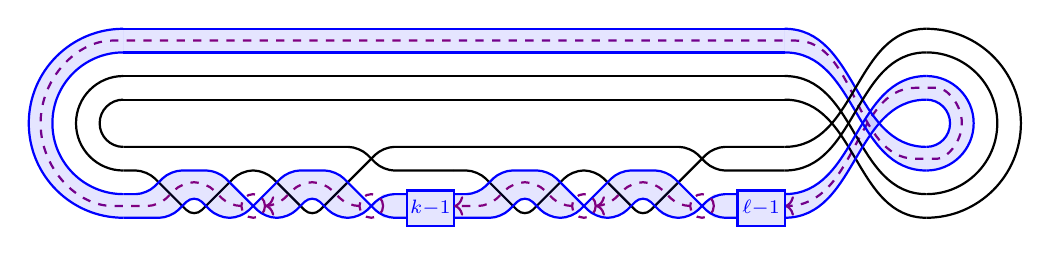
\begin{tikzpicture}[baseline=-.5ex, scale=0.6]
\begin{scope}
\draw[thick] (-7, 0.5) -- ++(7,0) (-7, 1) -- ++(7,0);
\draw[thick, blue] (-7, 1.5) -- ++(7,0) (-7, 2) -- ++(7,0);
\fill[blue, opacity=0.1] (-7, 1.5) -- ++(7,0) -- ++(0, 0.5) -- ++(-7, 0);
%
\draw[thick, rounded corners] (-7, -0.5) -- ++(0.5, 0) -- ++(4.5, 0) -- ++(0.5, -0.5) -- ++(1,0) -- ++(0.5, 0);
\draw[thick, rounded corners] (-7, -1) -- ++(0.5, 0) -- ++(1, -1) -- ++(1, 1) -- ++(0.5, 0) -- ++(1, -1) -- ++(1.5, 1.5) -- ++(1, 0) -- ++(0.5, 0);
\draw[thick, blue, rounded corners] (-7, -1.5) -- ++(0.5, 0) -- ++(0.5, 0.5) -- ++(1, 0) -- ++(1, -1) -- ++(0.5, 0) -- ++(0.5, 0.5) -- ++(0.5, -0.5) -- ++(0.5, 0) -- ++(0.5, 0.5) -- ++(0.5, 0);
\draw[thick, blue, rounded corners] (-7, -2) -- ++(0.5, 0) -- ++(0.5, 0) -- ++(0.5, 0.5) -- ++(0.5, -0.5) -- ++(0.5, 0) -- ++(1, 1) -- ++(1, 0) -- ++(1, -1) -- ++(0.5, 0);
\draw[thick, blue, fill=blue!10] (-1, -2.175) rectangle ++(1, 0.75) node[pos=.5] {$\scriptstyle k-1$};
\fill[blue, opacity=0.1] (-7, -2) [rounded corners]-- ++(0.5, 0) -- ++(0.5, 0) -- ++(0.5, 0.5) -- ++(0.5, -0.5) -- ++(0.5, 0) [sharp corners]-- ++(0.25, 0.25) 
[rounded corners]-- ++(-0.75, 0.75) -- ++(-1, 0) -- ++(-0.5, -0.5) -- ++(-0.5, 0);
\fill[blue, opacity=0.1] (-4.25, -1.75) [rounded corners]-- ++(0.75, 0.75) -- ++(1, 0) [sharp corners]-- ++(0.75, -0.75)
[rounded corners]-- ++(-0.25, -0.25) -- ++(-0.5, 0) -- ++(-0.5, 0.5) -- ++(-0.5, -0.5) -- ++(-0.5, 0) -- ++(-0.25, 0.25);
\fill[blue, opacity=0.1] (-1, -1.5) -- ++(-0.5, 0) -- ++(-0.25, -0.25) -- ++(0.25, -0.25) -- ++(0.5, 0);
%
\draw[thick, violet, dashed] 
(-4.25, -1.75) circle (0.25)
(-1.75, -1.75) circle (0.25)
;
\draw[thick, violet, dashed, ->, rounded corners]
(-2, -1.75) -- ++(-0.25, 0) -- ++(-0.5, 0.5) -- ++(-0.5, 0) -- ++(-0.5, -0.5) -- ++(-0.25, 0);
\draw[thick, violet, dashed, ->, rounded corners]
(-4.5, -1.75) -- ++(-0.25, 0) -- ++(-0.5, 0.5) -- ++(-0.5, 0) -- ++(-0.5, -0.5) -- ++(-0.75, 0) arc (-90:-270:1.75) -- ++(14, 0) to[out=0, in=180] ++(3, -2.5) arc (-90:90:0.75) to[out=180, in=0] ++(-3, -2.5);
%
\end{scope}
\begin{scope}[xshift=7cm]
\draw[thick] (-7, 0.5) -- ++(7,0) (-7, 1) -- ++(7,0);
\draw[thick, blue] (-7, 1.5) -- ++(7,0) (-7, 2) -- ++(7,0);
\fill[blue, opacity=0.1] (-7, 1.5) -- ++(7,0) -- ++(0, 0.5) -- ++(-7, 0);
%
\draw[thick, rounded corners] (-7, -0.5) -- ++(0.5, 0) -- ++(4.5, 0) -- ++(0.5, -0.5) -- ++(1,0) -- ++(0.5, 0);
\draw[thick, rounded corners] (-7, -1) -- ++(0.5, 0) -- ++(1, -1) -- ++(1, 1) -- ++(0.5, 0) -- ++(1, -1) -- ++(1.5, 1.5) -- ++(1, 0) -- ++(0.5, 0);
\draw[thick, blue, rounded corners] (-7, -1.5) -- ++(0.5, 0) -- ++(0.5, 0.5) -- ++(1, 0) -- ++(1, -1) -- ++(0.5, 0) -- ++(0.5, 0.5) -- ++(0.5, -0.5) -- ++(0.5, 0) -- ++(0.5, 0.5) -- ++(0.5, 0);
\draw[thick, blue, rounded corners] (-7, -2) -- ++(0.5, 0) -- ++(0.5, 0) -- ++(0.5, 0.5) -- ++(0.5, -0.5) -- ++(0.5, 0) -- ++(1, 1) -- ++(1, 0) -- ++(1, -1) -- ++(0.5, 0);
\draw[thick, blue, fill=blue!10] (-1, -2.175) rectangle ++(1, 0.75) node[pos=.5] {$\scriptstyle \ell-1$};
\fill[blue, opacity=0.1] (-7, -2) [rounded corners]-- ++(0.5, 0) -- ++(0.5, 0) -- ++(0.5, 0.5) -- ++(0.5, -0.5) -- ++(0.5, 0) [sharp corners]-- ++(0.25, 0.25) 
[rounded corners]-- ++(-0.75, 0.75) -- ++(-1, 0) -- ++(-0.5, -0.5) -- ++(-0.5, 0);
\fill[blue, opacity=0.1] (-4.25, -1.75) [rounded corners]-- ++(0.75, 0.75) -- ++(1, 0) [sharp corners]-- ++(0.75, -0.75)
[rounded corners]-- ++(-0.25, -0.25) -- ++(-0.5, 0) -- ++(-0.5, 0.5) -- ++(-0.5, -0.5) -- ++(-0.5, 0) -- ++(-0.25, 0.25);
\fill[blue, opacity=0.1] (-1, -1.5) -- ++(-0.5, 0) -- ++(-0.25, -0.25) -- ++(0.25, -0.25) -- ++(0.5, 0);
%
\draw[thick, violet, dashed] 
(-4.25, -1.75) circle (0.25)
(-1.75, -1.75) circle (0.25)
;
\draw[thick, violet, dashed, ->, rounded corners]
(-2, -1.75) -- ++(-0.25, 0) -- ++(-0.5, 0.5) -- ++(-0.5, 0) -- ++(-0.5, -0.5) -- ++(-0.25, 0);
\draw[thick, violet, dashed, ->, rounded corners]
(-4.5, -1.75) -- ++(-0.25, 0) -- ++(-0.5, 0.5) -- ++(-0.5, 0) -- ++(-0.5, -0.5) -- ++(-0.75, 0);
%
\end{scope}
\draw[thick] (-7, 0.5) arc (90:270:0.5) (-7, 1) arc (90:270:1);
\draw[thick, blue] (-7, 1.5) arc (90:270:1.5) (-7, 2) arc (90:270:2);
\fill[blue, opacity=0.1] (-7, 1.5) arc (90:270:1.5) -- (-7, -2) arc (-90:-270:2);
\begin{scope}
\draw[thick] (7, 1) to[out=0, in=180] ++(3, -2.5) (7, 0.5) to[out=0, in=180] ++(3, -2.5);
\draw[thick, blue] (7, 2) to[out=0, in=180] ++(3, -2.5) (7, 1.5) to[out=0, in=180] ++(3, -2.5);
\fill[blue, opacity=0.1] (7, 2) to[out=0, in=180] ++(3, -2.5) -- (10, -1) to[out=180, in=0] ++(-3, 2.5);
\end{scope}
\begin{scope}[yscale=-1]
\draw[thick] (7, 1) to[out=0, in=180] ++(3, -2.5) (7, 0.5) to[out=0, in=180] ++(3, -2.5);
\draw[thick, blue] (7, 2) to[out=0, in=180] ++(3, -2.5) (7, 1.5) to[out=0, in=180] ++(3, -2.5);
\fill[blue, opacity=0.1] (7, 2) to[out=0, in=180] ++(3, -2.5) -- (10, -1) to[out=180, in=0] ++(-3, 2.5);
\end{scope}
\draw[thick] (10, 2) arc (90:-90:2) (10, 1.5) arc (90:-90:1.5);
\draw[thick, blue] (10, 1) arc (90:-90:1) (10, 0.5) arc (90:-90:0.5);
\fill[blue, opacity=0.1] (10, 1) arc (90:-90:1) -- ++(0, 0.5) arc (-90:90:0.5);
%
\end{tikzpicture}
}
\caption{Legendrian Coxeter padding $\coxeterpadding({\exdynD}_{n})$ and the corresponding Legendrian loop $\vartheta_0({\exdynD}_{n})$}
\end{figure}

\begin{theorem}[Theorem~\ref{thm:legendrian loop}]\label{theorem:legendrian loop}
The Legendrian Coxeter mutation $\mutation_\ngraph$ on 
$(\ngraph(\exdynD),\nbasis(\exdynD))$ and twice of Legendrian mutation 
$\mutation_\ngraph^{2}$ on $(\ngraph(\exdynE),\nbasis(\exdynE))$ induce 
Legendrian loops $\vartheta(\exdynD)$ and $\vartheta(\exdynE)$ in Figures~\ref{fig:legendrian loop of E_intro} and \ref{fig:legendrian loop of D_intro}, respectively. 
In particular, the order of the Legendrian loops are infinite as elements of the fundamental group of the space of Legendrians isotopic to $\lambda(\exdynD)$ and $\lambda(\exdynE)$, respectively.
\end{theorem}

Note that the above idea of Coxeter mutation also works for $(\ngraph(a,b,c),\nbasis(a,b,c))$ with $\frac{1}{a}+\frac{1}{b}+\frac{1}{c} < 1$. Indeed the operation $\qcoxeter$ is of infinite order and so is $\ncoxeter$, hence Legendrian weaves 
\[\Legendrian(\ncoxeter^r(\ngraph(a,b,c),\nbasis(a,b,c)))\]
produce infinitely many distinct Lagrangian fillings.
The quiver $\quiver(a,b,c)$ is also bipartite and one can perform 
the Legendrian Coxeter mutation $\mutation_{\ngraph}$ on the $N$-graph $\ngraph(a,b,c)$ by stacking the gray-shaded annulus like as before. Therefore, there is no obstruction to
realize seeds obtained by mutations $\ncoxeter^r$ via the $N$-graphs.
Since the order of the Legendrian Coxeter mutation is infinite (see Lemma~\ref{lemma:order of coxeter mutation}), we obtain infinitely many $N$-graphs
and hence infinitely many exact embedded Lagrangian fillings for the Legendrian
link $\legendrian(a,b,c)$ with $\frac{1}{a}+\frac{1}{b}+\frac{1}{c} < 1$.

\begin{theorem}[Theorem~\ref{theorem:infinite fillings}]\label{thm_intro_infinite_fillings}
For each $a,b,c\ge 1$, the Legendrian knot or link $\legendrian(a,b,c)$ has 
infinitely many distinct Lagrangian fillings if
\[
\frac1a+\frac1b+\frac1c < 1.
\]
\end{theorem}

Gao--Shen--Weng \cite{GSW2020b} already proved the existence of infinitely many Lagrangian fillings for much general type of positive braid Legendrian links. Their main idea is to use the aperiodicity of \emph{Donaldson--Thomas transformation}(DT) on cluster varieties. An interesting observation is that the corresponding action of DT on the bipartite quivers in the $Y$-pattern becomes the Coxeter mutation. Accordingly, Theorem~\ref{thm_intro_infinite_fillings} can be interpreted as an $N$-graph analogue of the aperiodicity of DT.


\subsubsection{Lagrangian fillings for Legendrians of type $\dynBCFG$ or standard affine type with symmetry}
Now we move to cluster structure of type $\dynBCFG$ and standard affine types with certain symmetry.
They are obtained by the folding procedure from type $\dynADE$ or $\exdynD\exdynE$, see
Table~\ref{table:foldings}. 

In order to interpret those symmetries into Legendrians links and surfaces, we need to introduce corresponding actions on symplectic- and contact manifolds.
Consider two actions on $\sphere^3\times \R_u$, the rotation $R_{\theta_0}$ and conjugation  $\eta$ as follows:
\begin{align*}
R_{\theta_0}(z_1, z_2,u)&=(z_1\cos\theta_0 -z_2\sin\theta_0,z_1\sin\theta_0+z_2\cos\theta_0,u);\\
\eta(z_1,z_2,u)&= (\bar z_1,\bar z_2 ,u).
\end{align*}
Here $\sphere^3$ is the unit sphere in $\bbC^2$ with coordinates $z_1=r_1 e^{i\theta_1}, z_2=r_2 e^{i\theta_2}$ with $r_1^2 + r_2^2=1$.
Note that $\eta$ is an anti-symplectic involution which naturally gives $\Z/2\Z$-action on the symplectic manifold.
Under certain coordinate changes, the restrictions of $R_{\theta_0}$ and $\eta$ on $J^1\sphere^1$ become
\begin{align*}
R_{\theta_0}|_{J^1\sphere^1}(\theta,p_{\theta},z)&=(\theta+\theta_0,p_{\theta},z);\\
\eta|_{J^1\sphere^1}(\theta,p_{\theta},z)&=(\theta,-p_{\theta},-z).
\end{align*}
In turn, the rotation $R_{\theta_0}$ acts on the $N$-graph $\ngraph(\dynX)$ by rotating the disk $\disk^2$, and $\eta$ acts by flipping the $z$-coordinate.

Any $Y$-pattern of non-simply-laced finite or affine type can be obtained by folding 
a $Y$-pattern of type $\dynADE$ or $\exdynA \exdynD \exdynE$. In other words, 
those $Y$-pattern of non-simply-laced type can be seen as sub-patterns of $\dynADE$- or $\exdynA \exdynD \exdynE$-types 
consisting of $Y$-seeds with certain symmetries of finite group $G$ action. We call 
such $Y$-seeds or $N$-graphs \emph{$G$-admissible}, and the mutation in the folded 
cluster structure is a sequence of mutations respecting the $G$-orbits. 
We say that a $Y$-seed (or an $N$-graph) is \emph{globally foldable} if it is 
$G$-admissible and its arbitrary mutations along $G$-orbits are again 
$G$-admissible. 


Figure~\ref{figure:N-graph with rotational symmetry} illustrates the $N$-graphs with rotational symmetry and the corresponding $Y$-patterns of folding. Indeed, they are $\ngraph(1,n,n)$, $\ngraph(2,2,2)$, $\ngraph(3,3,3)$, $\ngraph(\exdynD_{2n})$, $\ngraph(\exdynD_4)$ which admits $\Z/2\Z$-, $\Z/3\Z$-, $\Z/3\Z$-, $\Z/2\Z$-, $\Z/2\Z$-action, respectively.

\begin{figure}[ht]
\[
\begin{tikzcd}[column sep=0.5pc, row sep=small]
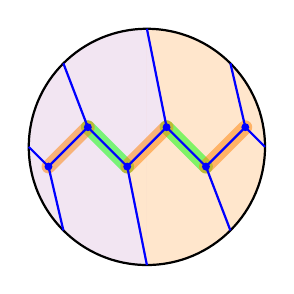
\begin{tikzpicture}[baseline=-.5ex,xscale=0.5,yscale=0.5]%B_3
\draw[orange, opacity=0.2, fill] (-90:3) arc(-90:90:3) (90:3) -- (0.5,0.5) -- (-0.5,-0.5) -- (-90:3);
\draw[violet, opacity=0.1, fill] (90:3) arc(90:270:3) (270:3) -- (-0.5,-0.5) -- (0.5,0.5) -- (90:3);
\draw[thick] (0,0) circle (3);
\draw[color=cyclecolor2,line cap=round, line width=5, opacity=0.5] (-1.5,0.5) -- (-0.5, -0.5) 
(0.5, 0.5) -- (1.5, -0.5);
\draw[color=cyclecolor1,line cap=round, line width=5, opacity=0.5] (-2.5,-0.5) -- (-1.5, 0.5) (-0.5, -0.5) -- (0.5, 0.5) (1.5, -0.5) -- (2.5, 0.5);
\draw[blue, thick, fill] (0:3) -- (2.5,0.5) circle (2pt) -- (45:3) (2.5,0.5) -- (1.5,-0.5) circle (2pt) -- (-45:3) (1.5,-0.5) -- (0.5,0.5) circle (2pt) -- (90:3) (0.5,0.5) -- (-0.5, -0.5) circle (2pt) -- (-90:3) (-0.5, -0.5) -- (-1.5, 0.5) circle (2pt) -- (135:3) (-1.5, 0.5) -- (-2.5, -0.5) circle (2pt) -- (-135:3);
\draw[blue, thick] (-2.5,-0.5) -- (-180:3);
\end{tikzpicture}
&
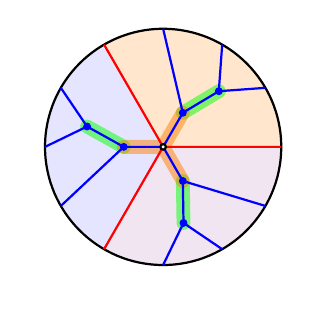
\begin{tikzpicture}[baseline=-.5ex,xscale=0.5,yscale=0.5]%G_2
\draw[orange, opacity=0.2, fill] (0:3) arc(0:120:3) (120:3) -- (0,0) -- (0:3);
\draw[violet, opacity=0.1, fill] (0:3) -- (0,0) -- (-120:3) arc(-120:0:3) (0:3);
\draw[blue, opacity=0.1, fill] (120:3) arc(120:240:3) (240:3) -- (0,0) -- (120:3);
\draw[thick] (0,0) circle (3cm);
\draw[color=cyclecolor2, line cap=round, line width=5, opacity=0.5] (60:1) -- (45:2)  (180:1) -- (165:2) (300:1) -- (285:2);
\draw[color=cyclecolor1, line cap=round, line width=5, opacity=0.5] (0,0) -- (60:1) (0,0) -- (180:1) (0,0) -- (300:1);
\draw[red, thick] (0,0) -- (0:3) (0,0) -- (120:3) (0,0) -- (240:3);
\draw[blue, thick, fill] 
(0,0) -- (60:1) circle (2pt) -- (90:3) 
(60:1) -- (45:2) circle (2pt) -- (30:3) 
(45:2) -- (60:3);
\draw[blue, thick, fill] 
(0,0) -- (180:1) circle (2pt) -- (210:3) 
(180:1) -- (165:2) circle (2pt) -- (150:3) 
(165:2) -- (180:3);
\draw[blue, thick, fill] 
(0,0) -- (300:1) circle (2pt) -- (330:3) 
(300:1) -- (285:2) circle (2pt) -- (270:3) 
(285:2) -- (300:3);
\draw[thick, fill=white] (0,0) circle (2pt);
\end{tikzpicture}
&
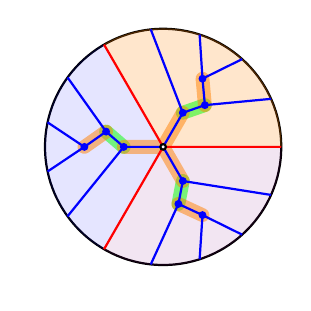
\begin{tikzpicture}[baseline=-.5ex,scale=0.5]
\draw[thick] (0,0) circle (3cm);
\draw[orange, opacity=0.2, fill] (0:3) arc(0:120:3) (120:3) -- (0,0) -- (0:3);
\draw[violet, opacity=0.1, fill] (0:3) -- (0,0) -- (-120:3) arc(-120:0:3) (0:3);
\draw[blue, opacity=0.1, fill] (120:3) arc(120:240:3) (240:3) -- (0,0) -- (120:3);
\draw[cyclecolor2, line cap=round, line width=5, opacity=0.5] (60:1) -- (45:1.5) (180:1) -- (165:1.5) (300:1) -- (285:1.5);
\draw[cyclecolor1, line cap=round, line width=5, opacity=0.5] (0,0) -- (60:1) (0,0) -- (180:1) (0,0) -- (300:1) (45:1.5) -- (60:2) (165:1.5) -- (180:2) (285:1.5) -- (300:2);
\draw[red, thick] (0,0) -- (0:3) (0,0) -- (120:3) (0,0) -- (240:3);
\draw[blue, thick, fill] (0,0) -- (60:1) circle (2pt) -- (96:3) (60:1) -- (45:1.5) circle (2pt) -- (24:3) (45:1.5) -- (60:2) circle (2pt) -- (72:3) (60:2) -- (48:3);
\draw[blue, thick, fill] (0,0) -- (180:1) circle (2pt) -- (216:3) (180:1) -- (165:1.5) circle (2pt) -- (144:3) (165:1.5) -- (180:2) circle (2pt) -- (192:3) (180:2) -- (168:3);
\draw[blue, thick, fill] (0,0) -- (300:1) circle (2pt) -- (336:3) (300:1) -- (285:1.5) circle (2pt) -- (264:3) (285:1.5) -- (300:2) circle (2pt) -- (312:3) (300:2) -- (288:3);
\draw[thick, fill=white] (0,0) circle (2pt);
\end{tikzpicture}
\\
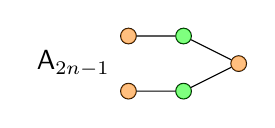
\begin{tikzpicture}[baseline=-.5ex,scale=0.7]
    
\node[Dnode] (a1) at (-2,0.5) {};
\node[Dnode] (a2) at (-1,0.5) {};
\node[Dnode] (a3) at (0,0) {};
\node[Dnode] (a4) at (-1,-0.5) {};
\node[Dnode] (a5) at (-2,-0.5) {};

\node[ynode] at (a1) {};
\node[gnode] at (a2) {};
\node[ynode] at (a3) {};
\node[gnode] at (a4) {};
\node[ynode] at (a5) {};

\draw (a1)--(a2)--(a3)--(a4)--(a5);

\node at (-3,0) {$\dynA_{2n-1}$};
\end{tikzpicture} 
&
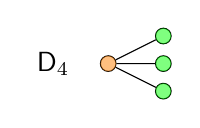
\begin{tikzpicture}[baseline=-.5ex,scale=0.7]
\coordinate[Dnode] (d1) at (-2,0) {};
\coordinate[Dnode] (d2) at  (-1,0)  {};
\coordinate[Dnode] (d3) at (-1,0.5) {};
\coordinate[Dnode] (d4) at (-1,-0.5) {};

\foreach \y in {d1} {
	\node[ynode] at (\y) {};
}
\foreach \g in {d2,d3,d4}{
	\node[gnode] at (\g) {};
}

\draw (d1)--(d2)
(d1)--(d3)
(d1)--(d4);

\node at (-3,0) {$\dynD_{4}$};

\end{tikzpicture} 
&
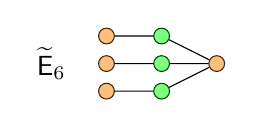
\begin{tikzpicture}[baseline=-.5ex,scale=0.7]    
\node[Dnode] (a1) at (0,0) {};
\node[Dnode] (a2) at (-1,0.5) {};
\node[Dnode] (a3) at (-2,0.5) {};
\node[Dnode] (a4) at (-1,0) {};
\node[Dnode] (a5) at (-2,0) {};
\node[Dnode] (a6) at (-1,-0.5) {};
\node[Dnode] (a7) at (-2,-0.5) {};

\node[ynode] at (a1) {};
\node[gnode] at (a2) {};
\node[ynode] at (a3) {};
\node[gnode] at (a4) {};
\node[ynode] at (a5) {};
\node[gnode] at (a6) {};
\node[ynode] at (a7) {};

\draw (a1)--(a2)--(a3) (a1)--(a4)--(a5) (a1)--(a6)--(a7);

\node at (-3,0) {$\exdynE_{6}$};

\end{tikzpicture}  \\[-1em]
\rotatebox{-90}{$\rightsquigarrow$}
& \rotatebox{-90}{$\rightsquigarrow$}
&\rotatebox{-90}{$\rightsquigarrow$} \\[-2em]
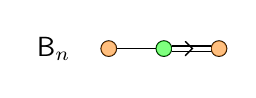
\begin{tikzpicture}[baseline=-.5ex,scale=0.7]

\node at (-3,0) {$\dynB_{n}$};

\coordinate[Dnode] (1) at (-2,0) {};
\coordinate[Dnode] (2) at (-1,0) {};
\coordinate[Dnode] (3) at (0,0) {};

\node[ynode] at (1) {};
\node[ynode] at (3) {};
\node[gnode] at (2) {};

\draw (1)--(2);
\draw[double line] (2)-- ++ (3); 

\end{tikzpicture}
&
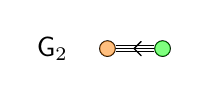
\begin{tikzpicture}[baseline=-.5ex,scale=0.7]
\node at (-3,0) {$\dynG_{2}$};
\coordinate[Dnode] (1) at (-2,0) {};
\coordinate[Dnode] (2) at (-1,0) {};

\node[ynode] at (1) {};
\node[gnode] at (2) {};

\draw[triple line] (2)-- ++ (1) ;
\draw (1)--(2);

\end{tikzpicture}
&
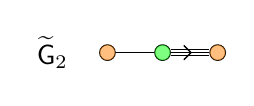
\begin{tikzpicture}[baseline=-.5ex,scale=0.7]
\node at (-3,0) {$\exdynG_{2}$};

\coordinate[Dnode] (3) at (-2,0) {};
\coordinate[Dnode] (2) at (-1,0) {};
\coordinate[Dnode] (1) at (0,0) {};

\node[ynode] at (1) {};
\node[gnode] at (2) {};
\node[ynode] at (3) {};

\draw (2)--(3);
\draw[triple line] (2)-- ++ (1) ;
\draw (1)--(2);

\end{tikzpicture}
\end{tikzcd}
\]

\[
\begin{tikzcd}[column sep=0.5pc, row sep=small]
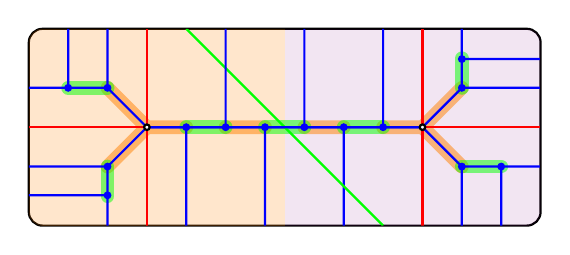
\begin{tikzpicture}[baseline=-.5ex,scale=0.5]
\draw[rounded corners=5, thick] (-6.5, -2.5) rectangle (6.5, 2.5);
\draw (0.5, -2.5) %node[above] {$\cdots$} 
(-0.5, -2.5) %node[below] {$\underbrace{\hphantom{\hspace{3cm}}}_{k-2}$}
;
\draw (1.5, 2.5) %node[below] {$\cdots$} 
(0.5, 2.5) %node[above] {$\overbrace{\hphantom{\hspace{3cm}}}^{k-2}$}
;
\clip[rounded corners=5] (-6.5, -2.5) rectangle (6.5, 2.5);
\draw[orange, opacity=0.2, fill] (0,2.5)--(-7,2.5)--(-7,-2.5)--(0,-2.5);
\draw[violet, opacity=0.1, fill] (0,2.5)--(7,2.5)--(7,-2.5)--(0,-2.5);
\draw[cyclecolor1, opacity=0.5, line cap=round, line width=5] 
(-3.5, 0) -- (-2.5, 0) (-3.5, 0) -- (-4.5, 1) (-3.5, 0) -- (-4.5, -1)
(-1.5, 0) -- (-0.5, 0)
(0.5, 0) -- (1.5, 0)
(3.5, 0) -- (2.5, 0) (3.5, 0) -- (4.5, 1) (3.5, 0) -- (4.5, -1)
;
\draw[cyclecolor2, opacity=0.5, line cap=round, line width=5] 
(-4.5, 1) -- (-5.5, 1)
(-4.5, -1) -- (-4.5, -1.75)
(-1.5, 0) -- (-2.5, 0)
(-0.5, 0) -- (0.5, 0)
(1.5, 0) -- (2.5, 0)
(4.5, 1) -- (4.5, 1.75)
(4.5, -1) -- (5.5, -1)
;
\foreach \i in {0, 180} {
\begin{scope}[rotate=\i]
\draw[thick, green] (-2.5, 2.5) -- (0,0);
\draw[thick, red] 
(-3.5, -2.5) -- (-3.5, 2.5)
(-6.5, 0) -- (-3.5, 0)
;
\draw[thick, blue, fill]
(-2.5, -2.5) -- (-2.5,0) circle (2pt)
(-0.5, -2.5) -- (-0.5,0) circle (2pt)
(1.5, -2.5) -- (1.5,0) circle (2pt)
;
\draw[thick, blue, fill] 
%
(-3.5, 0) -- (3.5, 0)
(-3.5, 0) -- (-4.5, 1) circle (2pt) -- (-4.5, 2.5)
(-4.5, 1) -- (-6.5, 1)
(-5.5, 1) circle (2pt) -- (-5.5, 2.5)
%
(-3.5, 0) -- (-4.5, -1) circle (2pt) -- (-4.5, -2.5)
(-4.5, -1) -- (-6.5, -1)
(-4.5, -1.73) circle (2pt) -- (-6.5, -1.73)
;
\end{scope}
}
\draw[thick, fill=white] (-3.5, 0) circle (2pt) (3.5, 0) circle (2pt);
\end{tikzpicture}
&
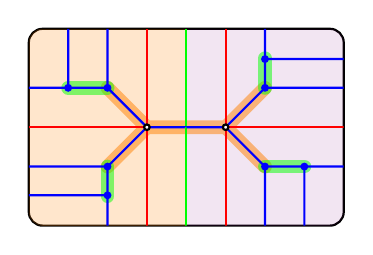
\begin{tikzpicture}[baseline=-.5ex,scale=0.5]
\draw[rounded corners=5, thick] (-4, -2.5) rectangle (4, 2.5);
\clip[rounded corners=5] (-4, -2.5) rectangle (4, 2.5);
\draw[orange, opacity=0.2, fill] (0,2.5)--(-7,2.5)--(-7,-2.5)--(0,-2.5);
\draw[violet, opacity=0.1, fill] (0,2.5)--(7,2.5)--(7,-2.5)--(0,-2.5);
\draw[cyclecolor1, opacity=0.5, line cap=round, line width=5]
(-1, 0) -- (1, 0) %node[near start, above, color=black, sloped,opacity=1] {$\cycle_1$} 
(-1, 0) -- (-2, 1) (-1, 0) -- (-2, -1)
(1, 0) -- (2, 1) (1, 0) -- (2, -1)
;
\draw[cyclecolor2, opacity=0.5, line cap=round, line width=5] 
(-2, 1) -- (-3, 1) %node[midway, below, color=black,opacity=1] {$\cycle_2$}
(-2, -1) -- (-2, -1.75) %node[midway, right=-1ex, color=black,opacity=1] {$\cycle_3$}
(2, 1) -- (2, 1.75) %node[midway, left=-1ex, color=black,opacity=1] {$\cycle_4$}
(2, -1) -- (3, -1) %node[midway, above, color=black,opacity=1] {$\cycle_5$}
;
\foreach \i in {0, 180} {
\begin{scope}[rotate=\i]
\begin{scope}[xshift=2.5cm]
\draw[thick, green] (-2.5, 2.5) -- ++(0,-2.5);
\draw[thick, red] 
(-3.5, -2.5) -- (-3.5, 2.5)
(-6.5, 0) -- (-3.5, 0)
;
\draw[thick, blue, fill] 
%
(-3.5, 0) -- (-2.5, 0)
(-3.5, 0) -- (-4.5, 1) circle (2pt) -- (-4.5, 2.5)
(-4.5, 1) -- (-6.5, 1)
(-5.5, 1) circle (2pt) -- (-5.5, 2.5)
%
(-3.5, 0) -- (-4.5, -1) circle (2pt) -- (-4.5, -2.5)
(-4.5, -1) -- (-6.5, -1)
(-4.5, -1.73) circle (2pt) -- (-6.5, -1.73)
;
\end{scope}
\end{scope}
}
\draw[thick, fill=white] (-1, 0) circle (2pt) (1, 0) circle (2pt);
\end{tikzpicture}
\\
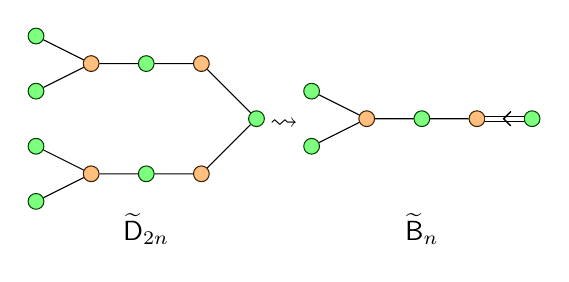
\begin{tikzpicture}[baseline=-.5ex,scale=0.7]

\coordinate[Dnode] (d1) at (0,1.5) {};
\coordinate[Dnode] (d2) at (0,0.5) {};
\coordinate[Dnode] (d3) at (1,1) {};
\coordinate[Dnode] (d4) at (2,1) {};
\coordinate[Dnode] (d5) at (3,1) {};
\coordinate[Dnode] (d6) at (0,-0.5) {};
\coordinate[Dnode] (d7) at (0,-1.5) {};
\coordinate[Dnode] (d8) at (1,-1) {};
\coordinate[Dnode] (d9) at (2,-1) {};
\coordinate[Dnode] (d10) at (3,-1) {};
\coordinate[Dnode] (d11) at (4,0) {};

\node[gnode] at (d1) {};
\node[gnode] at (d2) {};
\node[gnode] at (d4) {};
\node[gnode] at (d6) {};
\node[gnode] at (d7) {};
\node[gnode] at (d9) {};
\node[gnode] at (d11) {};

\node[ynode] at (d3) {};
\node[ynode] at (d5) {};
\node[ynode] at (d8) {};
\node[ynode] at (d10) {};

\draw  (d1)--(d3)--(d4)--(d5)--(d11)--(d10)--(d9)--(d8)--(d6)
(d2)--(d3) (d7)--(d8);

\node at (2,-2) {$\exdynD_{2n}$};
\node at (4.5,-0.1) {$\rightsquigarrow$};

\begin{scope}[xshift=5cm]
\node at (2,-2) {$\exdynB_{n}$};
\coordinate[Dnode] (1) at (0,0.5) {};
\coordinate[Dnode] (2) at (0,-0.5) {};
\coordinate[Dnode] (3) at (1,0) {};
\coordinate[Dnode] (4) at (2,0) {};
\coordinate[Dnode] (5) at (3,0) {};
\coordinate[Dnode] (6) at (4,0) {};

\node[gnode] at (1) {};
\node[gnode] at (2) {};
\node[ynode] at (3) {};
\node[gnode] at (4) {};
\node[ynode] at (5) {};
\node[gnode] at (6) {};

\draw (1)--(3)--(4)--(5) (2)--(3) ;
\draw[double line] (6)-- ++ (5) ;
\end{scope}

\end{tikzpicture}
&
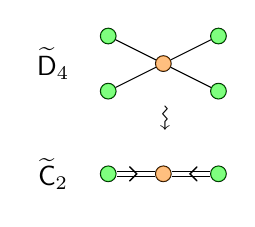
\begin{tikzpicture}[baseline=-.5ex,scale=0.7]

\coordinate[Dnode] (d1) at (0,0) {};
\coordinate[Dnode] (d2) at (-1,0.5) {};
\coordinate[Dnode] (d3) at (-1,-0.5) {};
\coordinate[Dnode] (d4) at (1,0.5) {};
\coordinate[Dnode] (d5) at (1,-0.5) {};

\node[ynode] at (d1) {};
\node[gnode] at (d3) {};
\node[gnode] at (d2) {};
\node[gnode] at (d4) {};
\node[gnode] at (d5) {};

\draw (d4)--(d1)--(d2) (d3)--(d1)--(d5);

\node at (-2,0) {$\exdynD_{4}$};
\node at (0,-1) {\rotatebox[origin=c]{-90}{$\rightsquigarrow$}};

\node at (-2,-2) {$\exdynC_{2}$};
\coordinate[Dnode] (c1) at (-1,-2) {};
\coordinate[Dnode] (c2) at (-0,-2) {};
\coordinate[Dnode] (c3) at (1,-2) {};

\node[gnode] at (c1) {};
\node[ynode] at (c2) {};
\node[gnode] at (c3) {};

\draw[double line] (c3)-- ++ (c2);
\draw[double line] (c1)-- ++ (c2);

\end{tikzpicture}
\end{tikzcd}
\]
\caption{Examples of $N$-graphs with rotational symmetry}
\label{figure:N-graph with rotational symmetry}
\end{figure}

In order to present conjugation invariant $N$-graphs, we need to adopt a degenerate version of $N$-graphs which allows overlapping edges and cycles as in Figure~\ref{figure:N-graph with conjugation symmetry}.
They are equivalent to $\ngraph(\exdynD_{n+1})$, $\ngraph(\exdynD_4)$, $\ngraph(2,3,3)$, $\ngraph(3,3,3)$, and $\ngraph(2,4,4)$ up to $\partial$-Legendrian isotopy see Definition~\ref{def:boundary Legendrian isotopic}, respectively.

\begin{figure}[ht]
\[
\begin{tikzcd}[column sep=0.5pc, row sep=small]
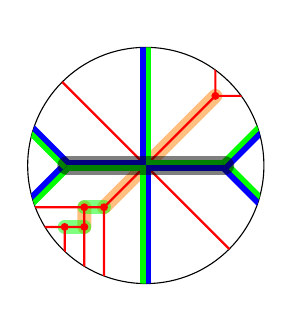
\begin{tikzpicture}[baseline=-.5ex, scale=0.5]
\useasboundingbox (-3, -3.5) rectangle (3, 3.5);
\draw (0,0) circle (3);
\clip (0,0) circle (3);
\draw[color=cyclecolor1,line cap=round, line width=5, opacity=0.5](-135:1.5)--(45:2.5)
(-135:1.5) ++(-0.5,0) -- ++(0,-0.5);
\draw[color=cyclecolor2,line cap=round, line width=5, opacity=0.5](-135:1.5)-- ++(-0.5,0)
(-135:1.5) ++(-0.5,-0.5) -- ++(-0.5,0);
\draw[fill, red, thick]
(3,-3) -- (0,0) 
(0,0) -- (-3,3)
(0,0) -- (45:2.5) circle (2pt)
(45:2.5) -- ++(0,3) (45:2.5) -- ++(3,0)
(0,0) -- (-135:1.5) circle (2pt)
(-135:1.5) -- ++(0,-3)
(-135:1.5) -- ++(-3,0)
(-135:1.5) ++ (-.5,0) circle (2pt) -- ++(0,-2)
(-135:1.5) ++ (-.5,-.5) circle (2pt) -- ++(-2,0)
(-135:1.5) ++ (-1,-.5) circle (2pt)
(-135:1.5) ++ (-1,-.5) -- ++(0,-1);
%
\draw[Dble={green and blue},line width=2] (-2,0) -- ++(-1,-1);
\draw[Dble={green and blue},line width=2] (-2,0) -- ++(-1,1);
\draw[Dble={blue and green},line width=2] (-2,0) -- (0,0);
\draw[Dble={blue and green},line width=2] (0,0) -- (0,3);
\draw[Dble={blue and green},line width=2] (0,0) -- (0,-3);
\draw[Dble={green and blue},line width=2] (0,0) -- (2,0);
\draw[Dble={green and blue},line width=2] (2,0) -- ++(2,-2);
\draw[Dble={green and blue},line width=2] (2,0) -- ++(2,2);

\draw[color=cyclecolor3,line width=7,opacity=0.5,line cap=round](-2,0)--(2,0);
%
\end{tikzpicture}
&
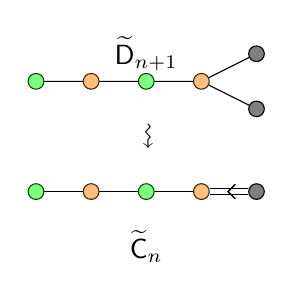
\begin{tikzpicture}[baseline=-5ex,scale=0.7]

\coordinate[Dnode] (d1) at (0,0) {};
\coordinate[Dnode] (d2) at (1,0) {};
\coordinate[Dnode] (d3) at (2,0) {};
\coordinate[Dnode] (d4) at (3,0) {};
\coordinate[Dnode] (d5) at (4,0.5) {};
\coordinate[Dnode] (d6) at (4,-0.5) {};

\node[gnode] at (d1) {};
\node[ynode] at (d2) {};
\node[gnode] at (d3) {};
\node[ynode] at (d4) {};
\node[bnode] at (d5) {};
\node[bnode] at (d6) {};

\draw  (d1)--(d2)--(d3)--(d4)--(d5) (d4)--(d6);

\node at (2,0.5) {$\exdynD_{n+1}$};
\node at (2,-1) {\rotatebox[origin=c]{-90}{$\rightsquigarrow$}};

\begin{scope}[yshift=-2cm]
\node at (2,-1) {$\exdynC_{n}$};
\coordinate[Dnode] (1) at (0,0) {};
\coordinate[Dnode] (2) at (1,0) {};
\coordinate[Dnode] (3) at (2,0) {};
\coordinate[Dnode] (4) at (3,0) {};
\coordinate[Dnode] (5) at (4,0) {};

\node[gnode] at (1) {};
\node[ynode] at (2) {};
\node[gnode] at (3) {};
\node[ynode] at (4) {};
\node[bnode] at (5) {};

\draw (1)--(2)--(3)--(4) ;
\draw[double line] (5)-- ++ (4); 
\end{scope}
\end{tikzpicture}
&\hspace{6mm}&
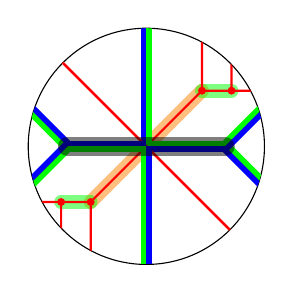
\begin{tikzpicture}[baseline=-.5ex, scale=0.5]
\draw (0,0) circle (3);
\clip (0,0) circle (3);
\draw[color=cyclecolor1,line cap=round, line width=5, opacity=0.5](-135:2)--(45:2);
\draw[color=cyclecolor2,line cap=round, line width=5, opacity=0.5](-135:2)-- ++(-0.75,0) (45:2)--++(0.75,0);
\foreach \r in {0, 180} {
\begin{scope}[rotate=\r]
\draw[fill, red, thick]
(3,-3) -- (-3,3) 
(0,0) -- (45:2) circle (2pt)
(45:2) -- ++(0,3)
(45:2) -- ++(3,0)
(45:2) ++ (0.75,0) circle (2pt) -- ++(0,2)
;
\draw[Dble={blue and green},line width=2] (0,0) -- (0,3);
\draw[Dble={green and blue},line width=2] (0,0) -- (2,0);
\draw[Dble={green and blue},line width=2] (2,0) -- ++(-45:2);
\draw[Dble={green and blue},line width=2] (2,0) -- ++(45:2);
\end{scope}
}
\draw[color=cyclecolor3,line width=7,opacity=0.5,line cap=round](-2,0)--(2,0);
\end{tikzpicture}
&
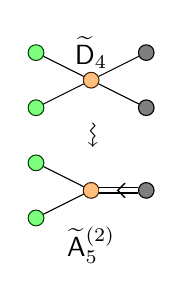
\begin{tikzpicture}[baseline=-5ex,scale=0.7]

\coordinate[Dnode] (d1) at (0,0) {};
\coordinate[Dnode] (d2) at (-1,0.5) {};
\coordinate[Dnode] (d3) at (-1,-0.5) {};
\coordinate[Dnode] (d4) at (1,0.5) {};
\coordinate[Dnode] (d5) at (1,-0.5) {};

\node[ynode] at (d1) {};
\node[gnode] at (d3) {};
\node[gnode] at (d2) {};
\node[bnode] at (d4) {};
\node[bnode] at (d5) {};

\draw (d4)--(d1)--(d2) (d3)--(d1)--(d5);

\node at (0,0.5) {$\exdynD_{4}$};
\node at (0,-1) {\rotatebox[origin=c]{-90}{$\rightsquigarrow$}};

\node at (0,-3) {$\exdynA_{5}^{(2)}$};
\coordinate[Dnode] (c1) at (-1,-1.5) {};
\coordinate[Dnode] (c2) at (0,-2) {};
\coordinate[Dnode] (c3) at (-1,-2.5) {};
\coordinate[Dnode] (c4) at (1,-2) {};

\node[gnode] at (c1) {};
\node[ynode] at (c2) {};
\node[gnode] at (c3) {};
\node[bnode] at (c4) {};

\draw (c1)--(c2)--(c3);
\draw[double line] (c4)-- ++ (c2);
\end{tikzpicture}
\end{tikzcd}
\]
\[
\begin{tikzcd}
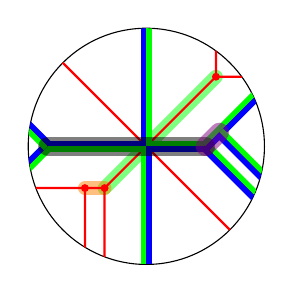
\begin{tikzpicture}[baseline=-.5ex, scale=0.5]
\draw (0,0) circle (3);
\clip (0,0) circle (3);
\draw[color=cyclecolor2,line cap=round, line width=5, opacity=0.5](-135:1.5)--(45:2.5);
\draw[color=cyclecolor1,line cap=round, line width=5, opacity=0.5](-135:1.5)--++(-0.5,0);
\draw[fill, red, thick]
(3,-3) -- (0,0) 
(0,0) -- (-3,3)
(0,0) -- (45:2.5) circle (2pt)
(45:2.5) -- ++(0,3) (45:2.5) -- ++(3,0)
(0,0) -- (-135:1.5) circle (2pt)
(-135:1.5) -- ++(0,-3)
(-135:1.5) -- ++(-3,0)
(-135:1.5) ++ (-0.5,0) circle (2pt) -- ++(0,-2);
%
\draw[Dble={green and blue},line width=2] (-2.5,0) -- ++(-1,-1);
\draw[Dble={green and blue},line width=2] (-2.5,0) -- ++(-1,1);
\draw[Dble={blue and green},line width=2] (-2.5,0) -- (0,0);
\draw[Dble={blue and green},line width=2] (0,0) -- (0,3);
\draw[Dble={blue and green},line width=2] (0,0) -- (0,-3);
\draw[Dble={green and blue},line width=2] (0,0) -- (1.5,0);
\draw[Dble={green and blue},line width=2] (1.5,0) -- ++(2,-2);
\draw[Dble={green and blue},line width=2] (1.5,0) -- ++(2,2);
\draw[Dble={green and blue},line width=2] (1.5,0) ++(45:0.5) -- ++(2,-2);

\draw[color=cyclecolor3,line width=7,opacity=0.5,line cap=round](-2.5,0)--(1.5,0);
\draw[color=cyclecolor4,line width=7,opacity=0.5,line cap=round](1.5,0)-- ++(45:0.5);
\end{tikzpicture} &
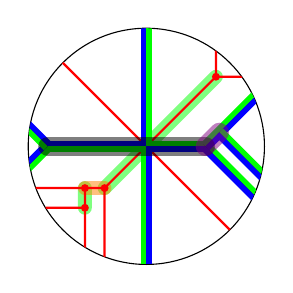
\begin{tikzpicture}[baseline=-.5ex, scale=0.5]
\draw (0,0) circle (3);
\clip (0,0) circle (3);
\draw[color=cyclecolor2,line cap=round, line width=5, opacity=0.5](-135:1.5)--(45:2.5) (-135:1.5)++(-0.5,0)--++(0,-0.5);
\draw[color=cyclecolor1,line cap=round, line width=5, opacity=0.5](-135:1.5)--++(-0.5,0);
\draw[fill, red, thick]
(3,-3) -- (0,0) 
(0,0) -- (-3,3)
(0,0) -- (45:2.5) circle (2pt)
(45:2.5) -- ++(0,3) (45:2.5) -- ++(3,0)
(0,0) -- (-135:1.5) circle (2pt)
(-135:1.5) -- ++(0,-3)
(-135:1.5) -- ++(-3,0)
(-135:1.5) ++ (-0.5,0) circle (2pt) -- ++(0,-2)
(-135:1.5) ++ (-0.5,0) ++(0,-0.5) circle (2pt) -- ++(-1, 0);
%
\draw[Dble={green and blue},line width=2] (-2.5,0) -- ++(-1,-1);
\draw[Dble={green and blue},line width=2] (-2.5,0) -- ++(-1,1);
\draw[Dble={blue and green},line width=2] (-2.5,0) -- (0,0);
\draw[Dble={blue and green},line width=2] (0,0) -- (0,3);
\draw[Dble={blue and green},line width=2] (0,0) -- (0,-3);
\draw[Dble={green and blue},line width=2] (0,0) -- (1.5,0);
\draw[Dble={green and blue},line width=2] (1.5,0) -- ++(2,-2);
\draw[Dble={green and blue},line width=2] (1.5,0) -- ++(2,2);
\draw[Dble={green and blue},line width=2] (1.5,0) ++(45:0.5) -- ++(2,-2);

\draw[color=cyclecolor3,line width=7,opacity=0.5,line cap=round](-2.5,0)--(1.5,0);
\draw[color=cyclecolor4,line width=7,opacity=0.5,line cap=round](1.5,0)-- ++(45:0.5);
\end{tikzpicture} &
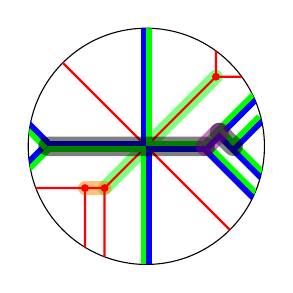
\begin{tikzpicture}[baseline=-.5ex, scale=0.5]
\draw (0,0) circle (3);
\clip (0,0) circle (3);
\draw[color=cyclecolor2,line cap=round, line width=5, opacity=0.5](-135:1.5)--(45:2.5);
\draw[color=cyclecolor1,line cap=round, line width=5, opacity=0.5](-135:1.5)--++(-0.5,0);
\draw[fill, red, thick]
(3,-3) -- (0,0) 
(0,0) -- (-3,3)
(0,0) -- (45:2.5) circle (2pt)
(45:2.5) -- ++(0,3) (45:2.5) -- ++(3,0)
(0,0) -- (-135:1.5) circle (2pt)
(-135:1.5) -- ++(0,-3)
(-135:1.5) -- ++(-3,0)
(-135:1.5) ++ (-0.5,0) circle (2pt) -- ++(0,-2);
%
\draw[Dble={green and blue},line width=2] (-2.5,0) -- ++(-1,-1);
\draw[Dble={green and blue},line width=2] (-2.5,0) -- ++(-1,1);
\draw[Dble={blue and green},line width=2] (-2.5,0) -- (0,0);
\draw[Dble={blue and green},line width=2] (0,0) -- (0,3);
\draw[Dble={blue and green},line width=2] (0,0) -- (0,-3);
\draw[Dble={green and blue},line width=2] (0,0) -- (1.5,0);
\draw[Dble={green and blue},line width=2] (1.5,0) -- ++(2,-2);
\draw[Dble={green and blue},line width=2] (1.5,0) -- ++(2,2);
\draw[Dble={green and blue},line width=2] (1.5,0) ++(45:0.5) -- ++(2,-2);
\draw[Dble={green and blue},line width=2] (1.5,0) ++(45:0.5) ++(-45:0.5) -- ++(45:1);

\draw[color=cyclecolor3,line width=7,opacity=0.5,line cap=round](-2.5,0)--(1.5,0) (1.5,0)++(45:0.5) -- ++(-45:0.5);
\draw[color=cyclecolor4,line width=7,opacity=0.5,line cap=round](1.5,0)-- ++(45:0.5);
\end{tikzpicture}
\\
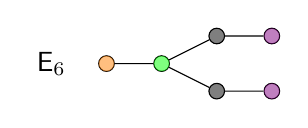
\begin{tikzpicture}[baseline=-0.5ex,scale=0.7]

\coordinate[Dnode] (d1) at (1,0) {};
\coordinate[Dnode] (d2) at (2,0) {};
\coordinate[Dnode] (d3) at (3,0.5) {};
\coordinate[Dnode] (d4) at (4,0.5) {};
\coordinate[Dnode] (d5) at (3,-0.5) {};
\coordinate[Dnode] (d6) at (4,-0.5) {};

\node[ynode] at (d1) {};
\node[gnode] at (d2) {};
\node[bnode] at (d3) {};
\node[vnode] at (d4) {};
\node[bnode] at (d5) {};
\node[vnode] at (d6) {};

\draw  (d1)--(d2)--(d3)--(d4) (d2)--(d5)--(d6);

\node at (0,0) {$\dynE_{6}$};
\end{tikzpicture} 
&
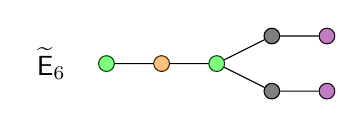
\begin{tikzpicture}[baseline=-0.5ex,scale=0.7]

\coordinate[Dnode] (d0) at (0,0) {};
\coordinate[Dnode] (d1) at (1,0) {};
\coordinate[Dnode] (d2) at (2,0) {};
\coordinate[Dnode] (d3) at (3,0.5) {};
\coordinate[Dnode] (d4) at (4,0.5) {};
\coordinate[Dnode] (d5) at (3,-0.5) {};
\coordinate[Dnode] (d6) at (4,-0.5) {};

\node[gnode] at (d0) {};
\node[ynode] at (d1) {};
\node[gnode] at (d2) {};
\node[bnode] at (d3) {};
\node[vnode] at (d4) {};
\node[bnode] at (d5) {};
\node[vnode] at (d6) {};

\draw  (d0)--(d1)--(d2)--(d3)--(d4) (d2)--(d5)--(d6);

\node at (-1,0) {$\exdynE_{6}$};
\end{tikzpicture}
&
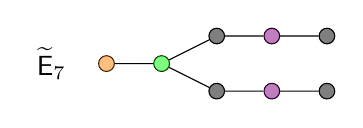
\begin{tikzpicture}[baseline=-0.5ex,scale=0.7]

\coordinate[Dnode] (d1) at (1,0) {};
\coordinate[Dnode] (d2) at (2,0) {};
\coordinate[Dnode] (d3) at (3,0.5) {};
\coordinate[Dnode] (d4) at (4,0.5) {};
\coordinate[Dnode] (d5) at (3,-0.5) {};
\coordinate[Dnode] (d6) at (4,-0.5) {};
\coordinate[Dnode] (d7) at (5,0.5) {};
\coordinate[Dnode] (d8) at (5,-0.5) {};

\node[ynode] at (d1) {};
\node[gnode] at (d2) {};
\node[bnode] at (d3) {};
\node[vnode] at (d4) {};
\node[bnode] at (d5) {};
\node[vnode] at (d6) {};
\node[bnode] at (d7) {};
\node[bnode] at (d8) {};

\draw  (d1)--(d2)--(d3)--(d4)--(d7) (d2)--(d5)--(d6)--(d8);

\node at (0,0) {$\exdynE_{7}$};
\end{tikzpicture}\\[-1em]
\rotatebox{-90}{$\rightsquigarrow$}
& \rotatebox{-90}{$\rightsquigarrow$}
&\rotatebox{-90}{$\rightsquigarrow$} \\[-2em]
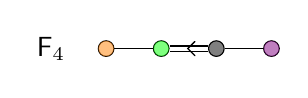
\begin{tikzpicture}[baseline=-0.5ex,scale=0.7]
\node at (0,0) {$\dynF_{4}$};
\coordinate[Dnode] (1) at (1,0) {};
\coordinate[Dnode] (2) at (2,0) {};
\coordinate[Dnode] (3) at (3,0) {};
\coordinate[Dnode] (4) at (4,0) {};

\node[ynode] at (1) {};
\node[gnode] at (2) {};
\node[bnode] at (3) {};
\node[vnode] at (4) {};

\draw (1)--(2) (3)--(4) ;
\draw[double line] (3)-- ++ (2);
\end{tikzpicture}  
&
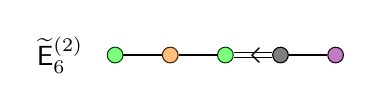
\begin{tikzpicture}[baseline=-0.5ex,scale=0.7]
\node at (-1,0) {$\exdynE_{6}^{(2)}$};
\coordinate[Dnode] (0) at (0,0) {};
\coordinate[Dnode] (1) at (1,0) {};
\coordinate[Dnode] (2) at (2,0) {};
\coordinate[Dnode] (3) at (3,0) {};
\coordinate[Dnode] (4) at (4,0) {};

\node[gnode] at (0) {};
\node[ynode] at (1) {};
\node[gnode] at (2) {};
\node[bnode] at (3) {};
\node[vnode] at (4) {};

\draw (0)--(1)--(2) (3)--(4) ;
\draw[double line] (3)-- ++ (2) ;
\end{tikzpicture}
&
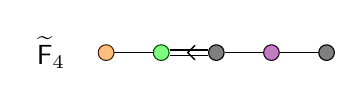
\begin{tikzpicture}[baseline=-0.5ex,scale=0.7]
\node at (0,0) {$\exdynF_{4}$};
\coordinate[Dnode] (1) at (1,0) {};
\coordinate[Dnode] (2) at (2,0) {};
\coordinate[Dnode] (3) at (3,0) {};
\coordinate[Dnode] (4) at (4,0) {};
\coordinate[Dnode] (5) at (5,0) {};

\node[ynode] at (1) {};
\node[gnode] at (2) {};
\node[bnode] at (3) {};
\node[vnode] at (4) {};
\node[bnode] at (5) {};

\draw (1)--(2) (3)--(4)--(5) ;
\draw[double line] (3)-- ++ (2) ;
\end{tikzpicture}
\end{tikzcd}
\]
\caption{Examples of $N$-graphs with conjugation symmetry}
\label{figure:N-graph with conjugation symmetry}
\end{figure}

\begin{theorem}[Theorem~\ref{thm:folding of N-graphs}]\label{Thm:folding of N-graphs}
The following holds:
\begin{enumerate}
\item The Legendrian $\lambda(\dynA_{2n-1})$ has $\binom{2n}{n}$ Lagrangian fillings which are invariant under the $\pi$-rotation and  admit the $Y$-pattern of type $\dynB_n$.
\item The Legendrian $\lambda(\dynD_{4})$ has $8$ Lagrangian fillings which are invariant under the $2\pi/3$-rotation and admit the $Y$-pattern of type $\dynG_2$.
\item The Legendrian $\lambda(\exdynE_{6})$ has Lagrangian fillings which are invariant under the $2\pi/3$-rotation and admit the $Y$-pattern of type $\exdynG_2$.
\item The Legendrian $\lambda(\exdynD_{2n})$ with $n\ge 3$ has Lagrangian fillings which are invariant under the $\pi$-rotation and admit the $Y$-pattern of type $\exdynB_n$.
\item The Legendrian $\lambda(\exdynD_4)$ has Lagrangian fillings which are invariant under the $\pi$-rotation and admit the $Y$-pattern of type $\exdynC_2$.
%
\item The Legendrian $\tilde\lambda(\dynE_{6})$ has $105$ Lagrangian fillings which are invariant under the antisymplectic involution and admit the $Y$-pattern of type $\dynF_4$.
\item The Legendrian $\tilde\lambda(\dynD_{n+1})$ has $\binom{2n}{n}$ Lagrangian fillings which are invariant under the antisymplectic involution and admit the $Y$-pattern of type $\dynC_n$.
\item The Legendrian $\tilde\lambda(\exdynE_{6})$ has Lagrangian fillings which are invariant under the antisymplectic involution and admit the $Y$-pattern of type $\dynE_6^{(2)}$.
\item The Legendrian $\tilde\lambda(\exdynE_{7})$ has Lagrangian fillings which are invariant under the antisymplectic involution and admit the $Y$-pattern of type $\exdynF_4$.
\item The Legendrian $\tilde\lambda(\exdynD_4)$ has Lagrangian fillings which are invariant under the antisymplectic involution and admit the $Y$-pattern of type $\dynA_5^{(2)}$.
\end{enumerate}
\end{theorem}

The study of Lagrangian fillings with symmetry, again to the best of authors' knowledge, is started from \cite{Cas2020}. We clarify the actions on the symplectic and contact manifold, together with the induced actions on Lagrangian fillings and Legendrian links. The items (1),(2),(6),(7) in Theorem~\ref{Thm:folding of N-graphs} answer that the conjecture \cite[Conjecture 5.4]{Cas2020} is true, and furthermore we extend our results to certain non-simply-laced affine types.


\subsection{Organization of the paper}
The rest of the paper is divided into six sections including appendices. 
We review, in Section~\ref{sec:cluster algebras}, some basics on finite and affine cluster algebra. Especially we focus on structural results about the combinatorics of exchange graphs using Coxeter mutations.

In Section~\ref{sec:N-graph}, we recall how $N$-graphs and their moves encode Legendrian surfaces and the Legendrian isotopies. We also introduce degenerate $N$-graphs which will be used to construct Lagrangian fillings having conjugation symmetry. 
After that we review the assignment of $Y$-seeds in the cluster structure from $N$-graphs together with certain flag moduli. We also discuss the Legendrian mutation on (degenerate) $N$-graphs.

In Section~\ref{sec:N-graph of finite or affine type}, we investigate Legendrian links and $N$-graphs of type $\dynADE$ or $\exdynD \exdynE$. 
We discuss $N$-graph realization of the Coxeter mutation and prove Theorem~\ref{theorem:legendrian loop} on the relationship between Coxeter mutations and Legendrian loops.
By combining the structural results in the seed pattern of cluster algebra and $N$-graph realization of the Coxeter mutation, we construct as many Lagrangian fillings as seeds for Legendrian links of type $\dynADE$ or $\exdynD \exdynE$, and hence prove Theorem~\ref{thm_intro_1}.

In Section~\ref{section:folding}, we discuss rotation and conjugation actions on $N$-graphs and invariant $N$-graphs. We also prove Theorem~\ref{Thm:folding of N-graphs}.

In Appendix~\ref{section:invariance and admissibility}, 
we argue that $G$-invariance of type $\dynADE$ implies $G$-admissibility. 
Finally, in Appendix~\ref{sec:supplementary pictorial proofs}, we collect several equivalences between different presentation of $N$-graphs.

If some readers are familiar with the notion of cluster algebra and $N$-graph, then one may skip Section~\ref{sec:cluster algebras} and Section~\ref{sec:N-graph}, respectively, and start from Section~\ref{sec:N-graph of finite or affine type}.


\subsection*{Acknowledgement}
B. An and Y. Bae were supported by the National Research Foundation of Korea (NRF) grant funded by the Korea government (MSIT) (No. 2020R1A2C1A0100320).
E. Lee was supported by the Institute for Basic Science (IBS-R003-D1).




\section{Cluster algebras}\label{sec:cluster algebras}
Cluster algebras, introduced by Fomin and Zelevinsky~\cite{FZ1_2002}, are
commutative algebras with specific generators, called \emph{cluster
	variables}, defined recursively.
In this section, we recall basic notions in the theory of cluster algebras.
For more details, we refer the reader to~\cite{FZ1_2002, FZ2_2003, FZ4_2007}.

Throughout this section, we fix $m, n \in \Z_{>0}$ such that $n \leq m$, and
we let $\field$ be the rational function field with $m$ independent
variables over $\bbC$.


\subsection{Basics on cluster algebras}


\begin{definition}[{cf. \cite{FZ1_2002, FZ2_2003, FZ4_2007}}]\label{definition:seeds}
A seed and $Y$-seed are defined as follows.
\begin{enumerate}
\item	A \emph{seed} $(\bfx, \qbasis)$ is a pair of 
	\begin{itemize}
		\item a tuple $\bfx = (x_1,\dots,x_m)$ of algebraically
		independent generators of $\field$, that is, 
		$\field = \bbC(x_1,\dots,x_m)$;
		\item an $m \times n$ integer matrix $\qbasis = (b_{i,j})_{i,j}$ such
		that the \emph{principal part} $\qbasispr \colonequals
		(b_{i,j})_{1\leq i,j\leq n}$ is skew-symmetrizable, that is, there
		exist positive integers $d_1,\dots,d_n$ such that
\[		
\textrm{diag}(d_1,\dots,d_n) \cdot \qbasispr 
\]
		is a
		skew-symmetric matrix.
	\end{itemize}
	We refer to $\bfx$ as the \emph{cluster} of a seed $(\bfx, \qbasis)$, to elements $x_1,\dots,x_m$ as \emph{cluster variables}, and to
	$\qbasis$ as the \emph{exchange matrix}. Moreover, we call $x_1,\dots,x_n$
	\emph{unfrozen} (or, \emph{mutable}) variables and $x_{n+1},\dots,x_m$
	\emph{frozen} variables.
\item A \emph{$Y$-seed} $(\bfy,\qbasispr)$ is a pair of an $n$-tuple $\bfy=(y_1,\dots,y_n)$ of elements in $\field$ and an $n\times n$ skew-symmetrizable matrix $\qbasispr$. 
We call $\bfy$ the \emph{coefficient tuple} of a $Y$-seed $(\bfy, \qbasispr)$ and call $y_1,\dots,y_n$ \emph{coefficients}.
\end{enumerate}
\end{definition}
We say that two seeds $(\bfx, \qbasis)$ and $(\bfx', \qbasis')$ are \textit{equivalent}, denoted by $(\bfx, \qbasis)\sim(\bfx', \qbasis')$ if there exists a permutation $\sigma$ on $[m]$ such that $\sigma|_{[n]}=[n]$, 
\[
x_i' = x_{\sigma(i)}\quad \text{ and } \quad b_{i,j}' = b_{\sigma(i),\sigma(j)} \quad \text{ for }1\le i\le m, 1\le j\le n,
\]
where $\bfx = (x_{1},\dots,x_{m})$, $\bfx' = (x_1',\dots,x_m')$, $\qbasis = (b_{i,j})$, and $\qbasis' = (b_{i,j}')$. Similarly,
two $Y$-seeds $(\bfy,\qbasispr)$ and $(\bfy',\qbasispr')$ are \emph{equivalent} and denoted by $(\bfy,\qbasispr)\sim(\bfy',\qbasispr')$ if there exists a permutation $\sigma$ on $[n]$ such that %$\sigma|_{[n]}=[n]$,
\[
y_i' = y_{\sigma(i)}\quad\text{and}\quad
b_{i,j}' = b_{\sigma(i),\sigma(j)}\quad\text{for }1\le i,j \le n.
\]

To define cluster algebras, we introduce mutations on exchange matrices, and quivers, and seeds as follows. 
\begin{enumerate}
\item (Mutation on exchange matrices)
For an exchange matrix $\qbasis$ and $1 \le k \le n$, the mutation $\mu_k(\qbasis) = (b_{i,j}')$ is defined as follows.
\[
b_{i,j}' = \begin{cases}
-b_{i,j} & \text{ if } i = k \text{ or } j = k, \\
\displaystyle b_{i,j} + \frac{|b_{i,k}| b_{k,j} + b_{i,k} | b_{k,j}|} {2} & \text{ otherwise}.
\end{cases}
\]
We say that \emph{$\qbasis' =(b_{i,j}')$ is the mutation of $\qbasis$ at $k$}.
\item (Mutation on quivers)
We call a finite directed multigraph $\quiver$ a \emph{quiver} if it does not have
oriented cycles of length at most $2$. The adjacency matrix $\qbasis(\quiver)$ of a
quiver is always skew-symmetric. Moreover, $\mu_k(\qbasis(\quiver))$ is again 
the adjacency matrix of a quiver $\quiver'$. We define $\mu_k(\quiver)$ to be 
the quiver satisfying 
\[
 \qbasis(\mu_k(\quiver)) = \mu_k(\qbasis(\quiver)),
\]
and say that \emph{$\mu_k(\quiver)$ is the mutation of $\quiver$ at $k$}.
\item (Mutation on seeds)	For a seed $(\bfx, \qbasis)$ and an integer $1 \leq k \leq n$, the \emph{mutation} $\mutation_k(\bfx, \qbasis) = (\bfx', \mu_k(\qbasis))$ is defined as follows: 
\begin{equation*}%\label{eq_mutation_on_seed_A}
x_i' = \begin{cases}
x_i &\text{ if } i \neq k,\\
\displaystyle 
x_k^{-1}\left( \prod_{b_{j,k} > 0} x_j^{b_{j,k}} + \prod_{b_{j,k} < 0}x_j^{-b_{j,k}}
\right) & \text{ otherwise}.
\end{cases}
\end{equation*}
\item (Mutation on $Y$-seeds)
The \emph{$Y$-seed mutation} (or, \emph{cluster $\mathcal{X}$-mutation}, \emph{$\mathcal{X}$-cluster mutation}) on a $Y$-seed $(\bfy, \qbasispr)$ at $k\in[n]$ is a $Y$-seed $(\bfy'=(y_1',\dots, y_n'),\qbasispr'=\mu_k(\qbasispr))$, where for each $1 \le i\le n$,
\[
y_i' = \begin{cases}
    \displaystyle {y}_{i} {y}_{k}^{\max\{b_{i,k},0\}}(1+{y}_{k})^{-b_{i,k}} & \text{ if }i \neq k, \\
   {y}_{k}^{-1} &\text{ otherwise}.
\end{cases}
\]


\end{enumerate}


\begin{example}\label{example_mutation_skewsymmetrizable}
Let $n = m = 2$. Suppose that an initial seed is given by
\[
(\bfx_{t_0}, \qbasis_{t_0}) = \left(
(x_1,x_2), \begin{pmatrix}
0 & 1 \\ -3 & 0
\end{pmatrix}
\right).
\]
Considering mutations $\mu_1(\bfx_{t_0}, \qbasis_{t_0})$ and $\mu_2\mu_1(\bfx_{t_0}, \qbasis_{t_0})$, we obtain the following.
\begin{align*}
\mu_1(\bfx_{t_0}, \qbasis_{t_0}) &= \left(
\left(
\frac{1+x_2^3}{x_1},x_2
\right), \begin{pmatrix}
0 & -1 \\3 & 0
\end{pmatrix}
\right),\\
\mu_2\mu_1(\bfx_{t_0}, \qbasis_{t_0}) &= \left(
\left(
\frac{1+x_2^3}{x_1}, \frac{1+x_1+x_2^3}{x_1x_2}
\right),
\begin{pmatrix}
0 & 1  \\ -3 & 0
\end{pmatrix}
\right).
\end{align*}
\end{example}


\begin{remark}\label{rmk_mutation_on_quivers}
Let $k$ be a vertex in a quiver $\quiver$ on $[m]$.
The mutation $\mutation_k(\quiver)$ can also be described via a sequence of three steps:
\begin{enumerate}
\item For each directed two-arrow path $i \to k \to j$, add a new arrow $i \to j$.
\item Reverse the direction of all arrows incident to the vertex $k$.
\item Repeatedly remove directed $2$-cycles until unable to do so.
\end{enumerate}
\end{remark}
\begin{remark}\label{rmk_mutation_commutes}
Let $\qbasis = (b_{i,j})$ be an exchange matrix of size $m \times n$.
For $k,\ell \in [n]$, if $b_{k,\ell} = b_{\ell,k} = 0$, then the mutations at $k$ and $\ell$ commute with each other: $\mutation_{\ell}(\mutation_k(\qbasis)) = \mutation_k(\mutation_{\ell}(\qbasis))$. 
Similarly, for a quiver $\quiver$ on $[m]$, if there does not exist an arrow connecting mutable vertices $k$ and $\ell$, then we have $\mutation_{\ell}(\mutation_k(\quiver)) = \mutation_k(\mutation_{\ell}(\quiver))$.
\end{remark}

We say a quiver $\quiver'$ is \emph{mutation equivalent} to another quiver $\quiver$ if 
there exists a sequence  of mutations $\mutation_{j_1},\dots,\mutation_{j_{\ell}}$ 
which connects $\quiver'$ and $\quiver$, that is,
\[
\quiver' = (\mutation_{j_{\ell}} \cdots \mutation_{j_1})(\quiver).
\]
Similarly, we say an exchange matrix $\qbasis'$ is \emph{mutation equivalent} to another matrix $\qbasis$ if $\qbasis'$ is obtained by applying a sequence of mutations to $\qbasis$. 


An immediate check shows that $\mutation_k(\bfx,\qbasis)$ is again a seed $\mutation_k(\bfy,\qbasispr)$ is a $Y$-seed, and a mutation is an involution, that is, its square is the identity.
Also, note that the mutation on seeds does not change frozen variables $x_{n+1},\dots,x_m$.
Let $\mathbb{T}_n$ denote the $n$-regular tree whose edges are labeled by $1,\dots,n$. Except for $n = 1$, there are infinitely many vertices on the tree $\mathbb{T}_n$. For example, we present regular trees $\mathbb{T}_2$ and $\mathbb{T}_3$ in Figure~\ref{figure_regular_trees_2_and_3}.
\begin{figure}
	\begin{tabular}{cc}
		
\begin{tikzpicture}
		\tikzset{every node/.style={scale=0.8}}
		\tikzset{cnode/.style = {circle, fill,inner sep=0pt, minimum size= 1.5mm}}
		\node[cnode] (1) {};
		\node[cnode, right of=1 ] (2) {};
		\node[cnode, right of=2 ] (3) {};
		\node[cnode, right of=3 ] (4) {};	
		\node[cnode, right of=4 ] (5) {};	
		\node[cnode, right of=5 ] (6) {};	
		
		\node[left of=1] {$\cdots$};
		\node[right of=6] {$\cdots$};
		
		\draw (1)--(2) node[above, midway] {$1$};
		\draw (2)--(3) node[above, midway] {$2$};
		\draw (3)--(4) node[above, midway] {$1$};
		\draw (4)--(5) node[above, midway] {$2$};
		\draw (5)--(6) node[above, midway] {$1$};
		\end{tikzpicture} &
		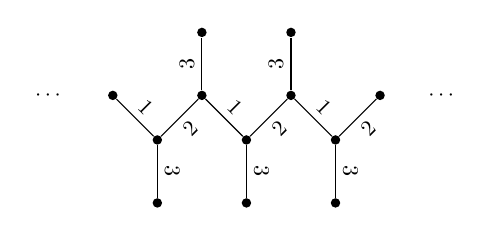
\begin{tikzpicture}
			\tikzset{every node/.style={scale=0.8}}
		\tikzset{cnode/.style = {circle, fill,inner sep=0pt, minimum size= 1.5mm}}
		\node[cnode] (1) {};
		\node[cnode, below right of =1] (2) {};
		\node[cnode, below of =2] (3) {};
		\node[cnode, above right of=2] (4){};
		\node[cnode, above of =4] (5) {};
		\node[cnode, below right of = 4] (6) {};
		\node[cnode, below of= 6] (7) {};
		\node[cnode, above right of = 6] (8) {};
		\node[cnode, above of = 8] (9) {};
		\node[cnode, below right of = 8] (10) {};
		\node[cnode, below of = 10] (11) {};
		\node[cnode, above right of = 10] (12) {};
		
		\node[left of = 1] {$\cdots$};
		\node[right of = 12] {$\cdots$};
		
		\draw (1)--(2) node[above, midway, sloped] {$1$};
		\draw (4)--(6) node[above, midway, sloped] {$1$};
		\draw (8)--(10) node[above, midway, sloped] {$1$};
		
		
		\foreach \x [evaluate ={ \x as \y using int(\x +2)} ] in {2, 6, 10}{
			\draw (\x)--(\y)  node[below, midway, sloped] {$2$}; 
		}
		\foreach \x [evaluate = {\x as \y using int(\x +1)}] in {2, 4, 6, 8, 10}{
			\draw (\x)--(\y) node[above, midway, sloped] {$3$};
		}
		\end{tikzpicture}\\[2ex]
		$\mathbb{T}_2$ & $\mathbb{T}_3$
	\end{tabular}
	\caption{The $n$-regular trees for $n=2$ and $n = 3$.}
	\label{figure_regular_trees_2_and_3}	
\end{figure}
A \emph{cluster pattern} (or \emph{seed pattern}) is an assignment
\[
\mathbb{T}_n \to \{\text{seeds in } \field\}, \quad t \mapsto (\bfx_t, \qbasis_t)
\]
such that if $\begin{tikzcd} t \arrow[r,dash, "k"] & t' \end{tikzcd}$ in $\mathbb{T}_n$, then $\mutation_k(\bfx_t, \qbasis_t) = (\bfx_{t'}, \qbasis_{t'})$.
Let $\{ (\bfx_t, \qbasis_t)\}_{t \in \mathbb{T}_n}$ be a cluster pattern with $\bfx_t = (x_{1;t},\dots,x_{m;t})$. Since the mutation does not change frozen variables, we may let $x_{n+1} = x_{n+1;t},\dots,x_m = x_{m;t}$.
\begin{definition}[{cf. \cite{FZ2_2003}}]
	Let $\{ (\bfx_t, \qbasis_t)\}_{t \in \mathbb{T}_n}$ be a cluster pattern with $\bfx_t = (x_{1;t},\dots,x_{m;t})$.
	The \emph{cluster algebra} $\cA(\{(\bfx_t, \qbasis_t)\}_{t \in \mathbb{T}_n})$ is defined to be the $\bbC[x_{n+1},\dots,x_m]$-subalgebra 
	of $\field$ generated by all the cluster variables 
	 $\bigcup_{t \in \mathbb{T}_n} \{x_{1;t},\dots,x_{n;t}\}$.
\end{definition}
If we fix a vertex $t_0 \in \mathbb{T}_n$, then a cluster pattern $\{ (\bfx_{t}, \qbasis_{t}) \}_{t \in \mathbb{T}_n}$ is 
constructed from the seed~$(\bfx_{t_0}, \qbasis_{t_0})$. In this case, we call $(\bfx_{t_0}, \qbasis_{t_0})$ an \emph{initial seed}. 
Because of this reason, we simply denote by $\cA(\bfx_{t_0}, \qbasis_{t_0})$ the cluster algebra given by the cluster 
pattern constructed from the initial seed~$(\bfx_{t_0}, \qbasis_{t_0})$.
\begin{example}\label{example_A2_example}
	Let $n = m = 2$. Suppose that an initial seed is given by 
	\[
		(\bfx_{t_0}, \qbasis_{t_0}) = \left(
			(x_1,x_2), \begin{pmatrix}
				0 & 1  \\ -1 & 0
			\end{pmatrix}
		\right).
	\]
	We present the cluster pattern obtained by the initial seed $(\bfx_{t_0}, \qbasis_{t_0})$.
	\begin{center}
	\begin{tikzcd}%[column sep = 0cm, row sep = 0cm]
		\left( (x_2,x_1), 
		\begin{pmatrix}
			0 & -1 \\ 1 & 0
		\end{pmatrix}
		\right)
		\arrow[r, color=white, "\textcolor{black}{\sim}" description]
		& (\bfx_{t_0}, \qbasis_{t_0})
			= \left(
			(x_1,x_2), 
			\begin{pmatrix}
				0 & 1 \\ -1 & 0
			\end{pmatrix}
		\right) \arrow[d,<->, "\mutation_1"]
		\\
		\left(
			(\frac{1+x_1}{x_2}, x_1), \begin{pmatrix}
				0 & 1 \\ -1 & 0
			\end{pmatrix}
		\right) \arrow[u,<->, "\mutation_1"]
		& 
		\left(
			\left(\frac{1+x_2}{x_1}, x_2\right), \begin{pmatrix}
				0 & -1 \\ 1 & 0
			\end{pmatrix}
		\right) \arrow[d, <->,"\mutation_2"]\\
		\left(
			\left(\frac{1+x_1}{x_2}, \frac{1+x_1+x_2}{x_1x_2}\right),
			\begin{pmatrix}
				0 & -1 \\ 1 & 0
			\end{pmatrix}
		\right) \arrow[u,<->, "\mutation_2"]
		&
		\left(
			\left(\frac{1+x_2}{x_1}, \frac{1+x_1+x_2}{x_1x_2}\right),
			\begin{pmatrix}
				0 & 1  \\ -1 & 0
			\end{pmatrix}
		\right) \arrow[l,<->, "\mutation_1"]
    \end{tikzcd}
\end{center}
Accordingly, we have
\[
\cA(\initialseed) = \cA(\{\seed_t\}_{t \in \mathbb{T}_n}) =  \bbC\left[x_1,x_2,\frac{1+x_2}{x_1}, \frac{1+x_1+x_2}{x_1x_2}, \frac{1+x_1}{x_2}\right].
\]
We notice that there are only five seeds in this case. Indeed, it becomes a cluster pattern of type~$\dynA_2$ (see Example~\ref{example_root_and_A2}).
\end{example}



\begin{remark}\label{rmk_x_cluster_mutation}
One can obtain a $Y$-pattern from a given cluster pattern as follows.
Let $\{ (\bfx_t, \qbasis_t)\}_{t \in \mathbb{T}_n}$ be a cluster
pattern with $\bfx_t = (x_{1;t},\dots,x_{m;t})$. For $t \in \mathbb{T}_n$ and
$i \in [n]$, we defined an assignment $(\mathbf x_t, \qbasis_t) \stackrel{\Theta}{\mapsto} (\hat{\mathbf y}_t,\qbasispr)$, where $\hat{\mathbf y}_t= (\hat{y}_{1;t},\dots,\hat{y}_{n;t})$ is defined by 
\[
    \hat{y}_{i;t} = \prod_{j\in[m] } x_{j;t}^{b^{(t)}_{i,j}}
\]
Here, $\qbasis_t = (b^{(t)}_{i,j})$ and $\qbasispr_t$ is the principal part of $\qbasis_t$.
Then the assignment $t \mapsto (\hat{\mathbf y}_t, \qbasispr)$ provides a 
$Y$-pattern and commutes with the mutation maps, indeed, we obtain $\mutation_k(\Theta(\mathbf x, \qbasis)) = \Theta(\mutation_k(\mathbf x,\qbasis))$. 
We notice that if the exchange matrix $\qbasis_t$ has full rank, then the variables $\hat{y}_{1;t},\dots,\hat{y}_{n;t}$ are algebraically independent. 
Note that the mutation preserves the rank of the exchange matrix as proved in~\cite[Lemma~3.2]{BFZ3_2005}.
\end{remark}


\subsection{Cluster algebras of Dynkin type}
The number of cluster variables in Example~\ref{example_A2_example} is finite
even though the number of vertices in the graph $\mathbb{T}_2$ is infinite.
We call such cluster algebras \emph{of finite type}. More precisely, we
recall the following definition.
\begin{definition}[{\cite{FZ2_2003}}]
	A cluster algebra is said to be \emph{of finite type} if it has finitely
	many cluster variables.
\end{definition}
It has been realized that classifying finite type cluster algebras is related
to studying exchange matrices. The \emph{Cartan counterpart}
$C(\qbasispr) = (c_{i,j})$ of the principal part
$\qbasispr$ of an exchange matrix $\qbasis$ is defined by
\[
c_{i,j} = \begin{cases}
2 & \text{ if } i = j, \\
-|b_{i,j}| & \text{ otherwise}.
\end{cases}
\]
Since $\qbasispr$ is skew-symmetrizable, its Cartan
counterpart $C(\qbasispr)$ is symmetrizable. 

We say that a quiver $\quiver$ is \emph{acyclic} if it does not have directed cycles.
Similarly, for a skew-symmetrizable matrix $\qbasispr = (b_{i,j})$, we say that it is \emph{acyclic} if there are no sequences $j_1,j_2,\dots,j_{\ell}$ with $\ell \ge 3$ such that
\[
b_{j_1,j_2}, b_{j_2,j_3},\dots,b_{j_{\ell-1},j_{\ell}},b_{j_{\ell},j_1} > 0.
\]
We say a seed $\seed = (\mathbf x, \qbasis)$ is \emph{acyclic} if so is its principal part $\qbasispr$.

\begin{definition}\label{def_quiver_of_type_X}
For a finite or affine Dynkin type $\dynX$, we define a quiver $\quiver$, a matrix $\qbasis$, a cluster pattern $\{(\bfx_t, \qbasis_t)\}_{t \in \mathbb{T}_n}$, a $Y$-pattern $\{(\bfy_t, \qbasispr_t)\}_{t \in \mathbb{T}_n}$, or a cluster algebra $\cA(\bfx_{t_0}, \qbasis_{t_0})$ \emph{of type~$\dynX$} as follows.
\begin{enumerate}
\item A quiver is \textit{of type~$\dynX$} 
if it is mutation equivalent to an \emph{acyclic} quiver whose underlying graph is isomorphic to the Dynkin 
diagram of type $\dynX$.
\item A skew-symmetrizable matrix $\qbasispr$ is \textit{of 
type $\dynX$} if it is mutation equivalent to an acyclic skew-symmetrizable matrix whose 
Cartan counterpart $C(\qbasispr)$ is isomorphic to the Cartan matrix of type~$\dynX$. 
\item A cluster pattern $\{(\bfx_t, \qbasis_t)\}_{t \in \mathbb{T}_n}$ or a $Y$-pattern $\{(\bfy_t, \qbasispr_t)\}_{t \in \mathbb{T}_n}$ is \textit{of type $\dynX$} if for some $t \in \mathbb{T}_n$, the Cartan counterpart  $C(\qbasispr_t)$ is of type $\dynX$.
\item A cluster algebra $\cA(\bfx_{t_0}, \qbasis_{t_0})$ is \textit{of type $\dynX$} if its cluster pattern is of type $\dynX$.
\end{enumerate}
\end{definition}

Here, we say that two matrices $C_1$ and $C_2$ are \emph{isomorphic} if they are conjugate to each other via a permutation matrix, that is, $C_2 = P^{-1} C_1 P$ for some permutation matrix~$P$. 
One may wonder whether there exist exchange matrices in the same seed pattern having different Dynkin type. 
However, it is proved in~\cite[Corollary~4]{CalderoKeller06} that if two acyclic skew-symmetrizable matrices are mutation equivalent, then there exists a sequence of mutations from one to other such that intermediate skew-symmetrizable matrices are all acyclic. Indeed, if two acyclic skew-symmetrizable matrices are mutation equivalent, then their Cartan counterparts are isomorphic. 

\begin{proposition}[{cf. \cite[Corollary~4]{CalderoKeller06}}]\label{prop_quiver_of_same_type_are_mutation_equivalent}
Let $\qbasispr$ and $\qbasispr'$ be acyclic skew-symmetrizable matrices. Then the following are equivalent:
\begin{enumerate}
\item the Cartan matrices $C(\qbasispr)$ and $C(\qbasispr')$ are isomorphic;
\item $\qbasispr$ and $\qbasispr'$ are mutation equivalent.
\end{enumerate}
\end{proposition}
Accordingly, a quiver, a matrix, a cluster pattern, or a cluster algebra of type $\dynX$ is well-defined. 
The following
theorem presents a classification of cluster algebras of finite type.
\begin{theorem}[{\cite{FZ2_2003}}] \label{thm_FZ_finite_type}
	Let $\{ (\bfx_t, \qbasis_t)\}_{t \in \mathbb{T}_n}$ be a
	cluster pattern with an initial seed $(\bfx_{t_0},
	\qbasis_{t_0})$. Let $\mathcal{A}(\bfx_{t_0}, \qbasis_{t_0})$ be the corresponding
	cluster algebra. Then, the cluster algebra $\mathcal{A}(\bfx_{t_0}, \qbasis_{t_0})$ is of finite type if and only if $\mathcal{A}(\bfx_{t_0}, \qbasis_{t_0})$ is of finite Dynkin type.
\end{theorem}



We provide a list of all of the irreducible finite type root systems and their Dynkin diagram in Table~\ref{table_finite}.
In Tables~\ref{table_standard_affine} and~\ref{table_twisted_affine}, we present lists of standard affine root 
systems and twisted affine root systems, respectively. They are the same as 
presented in Tables Aff 1, Aff 2, and Aff 3 of~\cite[Chapter~4]{Kac83}, and we 
denote by $\exdynX = \dynX^{(1)}$. 
We notice that the number of vertices of the standard affine Dynkin diagram of type $\exdynX_{n-1}$ is $n$ while we do not specify the vertex numbering. 

We note that all Dynkin diagram of finite or affine type but $\exdynA_{n-1}$ do not have (undirected) cycles. Accordingly, we may omit the acyclicity condition in Definition~\ref{def_quiver_of_type_X} except $\exdynA_{n-1}$-type. 
On the other hand, if a quiver is a directed $n$-cycle, then the corresponding Cartan counterpart is of type $\exdynA_{n-1}$ while it is mutation equivalent to a quiver of type $\dynD_n$ (see~Type IV in \cite{Vatne10}). 

The mutation equivalence classes of acyclic quivers of type $\exdynA_{n-1}$ are described in~\cite[Lemma~6.8]{FST08}. Let 
$\quiver$ and $\quiver'$ are two $n$-cycles for $n \geq 3$. Suppose that in 
$\quiver$, there are $p$ edges of one direction and $q = n - p$ edges of the 
opposite direction. Also, in $\quiver'$, there are $p'$ edges of one direction 
and $q' = n - p'$ edges of the opposite direction. Then two quivers $\quiver$ 
and $\quiver'$ are mutation equivalent if and only if the unordered pairs 
$\{p,q\}$ and $\{p',q'\}$ coincide. We say that a quiver 
$\quiver$ is of type $\exdynA_{p,q}$ if it has $p$ edges of one direction and 
$q$ edges of the opposite direction. We depict some examples for quivers of 
type $\exdynA_{p,q}$ in Figure~\ref{fig_example_Apq}.
%\end{remark}

\begin{figure}[ht]
\begin{tabular}{cccc}
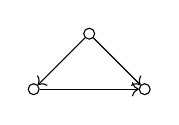
\begin{tikzpicture}[scale = 0.5]			
\tikzset{every node/.style={scale=0.7}}
\node[Dnode] (3) {};
\node[Dnode] (1) [below left = 0.6cm and 0.6cm of 3]{};
\node[Dnode] (2) [below right = 0.6cm and 0.6cm  of 3] {};

\draw[->] (3)--(1);
\draw[->] (3)--(2);
\draw[->] (1)--(2);
\end{tikzpicture} 
&	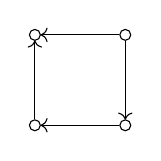
\begin{tikzpicture}[scale = 0.5]			
\tikzset{every node/.style={scale=0.7}}
\node[Dnode] (1) {};
\node[Dnode] (2) [below = of 1] {};
\node[Dnode] (3) [right = of 2] {};
\node[Dnode] (4) [above = of 3] {};

\draw[->] (4) -- (1);
\draw[->]	(4) -- (3);
\draw[->]	(3) -- (2);
\draw[->]	(2) --(1);
\end{tikzpicture} 
&	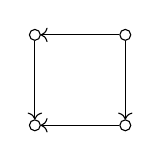
\begin{tikzpicture}[scale = 0.5]			
\tikzset{every node/.style={scale=0.7}}
\node[Dnode] (1) {};
\node[Dnode] (2) [below = of 1] {};
\node[Dnode] (3) [right = of 2] {};
\node[Dnode] (4) [above = of 3] {};

\draw[->] (4) -- (1);
\draw[->]	(4) -- (3);
\draw[->]	(3) -- (2);
\draw[->]	(1)--(2);
\end{tikzpicture} 
&
\raisebox{4em}{	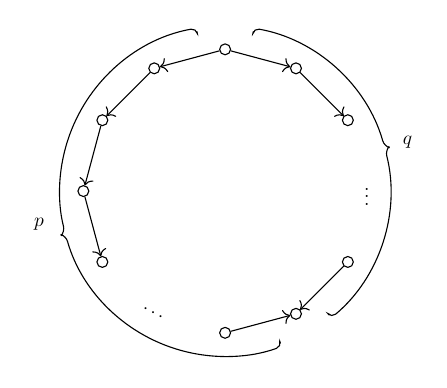
\begin{tikzpicture}[baseline=-.5ex,scale=0.6]
\tikzstyle{state}=[draw, circle, inner sep = 0.07cm]
\tikzset{every node/.style={scale=0.7}}
\foreach \x in {1,...,7, 9,10,11}{
\node[Dnode] (\x) at (\x*30:3) {};
}
\node(12) at (12*30:3) {$\vdots$};
\node[rotate=-30] (8) at (8*30:3) {$\cdots$};


\foreach \x [evaluate={\y=int(\x+1);}] in {3,...,6,9}{
\draw[->] (\x)--(\y);
}
\foreach \x [evaluate={\y=int(\x-1);}] in {3,2,11}{
\draw[->] (\x)--(\y);
} 
\curlybrace[]{100}{290}{3.5};
\draw (190:4) node[rotate=0] {$p$};
\curlybrace[]{-50}{80}{3.5};
\draw (15:4) node[rotate=0] {$q$};
\end{tikzpicture}}
\\	
$\exdynA_{1,2}$ & $\exdynA_{1,3}$ & $\exdynA_{2,2}$ & $\exdynA_{p,q}$
\end{tabular}
\caption{Quivers of type $\exdynA_{p,q}$.}\label{fig_example_Apq}
\end{figure}

In what follows, we fix an ordering on the simple roots as in Table~\ref{table_finite}; 
our conventions agree with that in the standard textbook of Humphreys~\cite{Humphreys}.


\begin{table}[t]
\begin{center}
\begin{tabular}{c|l  }
\toprule
$\Roots$ & Dynkin diagram \\
\midrule
$\dynA_n$ $(n \geq 1)$ &
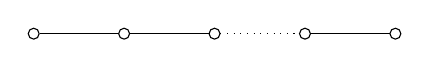
\begin{tikzpicture}[scale=.5, baseline=-.5ex]
	\tikzset{every node/.style={scale=0.7}}
	\node[Dnode] (1) {};
	\node[Dnode] (2) [right = of 1] {};
	\node[Dnode] (3) [right = of 2] {};
	\node[Dnode] (4) [right =of 3] {};
	\node[Dnode] (5) [right =of 4] {};			

	\draw (1)--(2)--(3)
		(4)--(5);
	\draw[dotted] (3)--(4);
\end{tikzpicture}  \\ 			
$\dynB_n$ $(n \geq 2)$ &
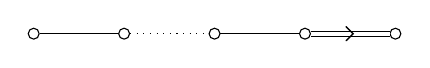
\begin{tikzpicture}[scale=.5, baseline=-.5ex]
	\tikzset{every node/.style={scale=0.7}}
			
	\node[Dnode] (1) {};
	\node[Dnode] (2) [right = of 1] {};
	\node[Dnode] (3) [right = of 2] {};
	\node[Dnode] (4) [right =of 3] {};
	\node[Dnode] (5) [right =of 4] {};

	\draw (1)--(2)
		(3)--(4);
	\draw [dotted] (2)--(3);
	\draw[double line] (4)--(5);
\end{tikzpicture}  \\ 			
$\dynC_n$ $(n \geq 3)$ & 
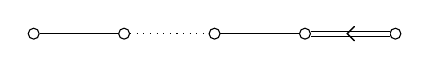
\begin{tikzpicture}[scale=.5, baseline=-.5ex]
	\tikzset{every node/.style={scale=0.7}}
			
	\node[Dnode] (1) {};
	\node[Dnode] (2) [right = of 1] {};
	\node[Dnode] (3) [right = of 2] {};
	\node[Dnode] (4) [right =of 3] {};
	\node[Dnode] (5) [right =of 4] {};

	\draw (1)--(2)
		(3)--(4);
	\draw [dotted] (2)--(3);
	\draw[double line] (5)--(4);
\end{tikzpicture}  \\ 
			
$\dynD_n$ $(n \geq 4)$ & 
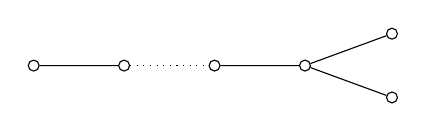
\begin{tikzpicture}[scale=.5, baseline=-.5ex]
	\tikzset{every node/.style={scale=0.7}}
			
	\node[Dnode] (1) {};
	\node[Dnode] (2) [right = of 1] {};
	\node[Dnode] (3) [right = of 2] {};
	\node[Dnode] (4) [right =of 3] {};			
			
	\node[Dnode] (5) [above right= 0.3cm and 1cm of 4] {};
	\node[Dnode] (6) [below right= 0.3cm and 1cm of 4] {};

	\draw(1)--(2)
		(3)--(4)--(5)
		(4)--(6);
	\draw[dotted] (2)--(3);
\end{tikzpicture}
\\ 
$\dynE_6$& 
\begin{tikzpicture}[scale=.5, baseline=-.5ex]
	\tikzset{every node/.style={scale=0.7}}

	\node[Dnode] (1) {};
	\node[Dnode] (3) [right=of 1] {};
	\node[Dnode] (4) [right=of 3] {};
	\node[Dnode] (2) [above=of 4] {};
	\node[Dnode] (5) [right=of 4] {};
	\node[Dnode] (6) [right=of 5]{};

	\draw(1)--(3)--(4)--(5)--(6)
		(2)--(4);
\end{tikzpicture}			
\\
$\dynE_7$ & 
\begin{tikzpicture}[scale=.5, baseline=-.5ex]
	\tikzset{every node/.style={scale=0.7}}

	\node[Dnode] (1) {};
	\node[Dnode] (3) [right=of 1] {};
	\node[Dnode] (4) [right=of 3] {};
	\node[Dnode] (2) [above=of 4] {};
	\node[Dnode] (5) [right=of 4] {};
	\node[Dnode] (6) [right=of 5]{};
	\node[Dnode] (7) [right=of 6]{};

	\draw(1)--(3)--(4)--(5)--(6)--(7)
		(2)--(4);
\end{tikzpicture}	
\\
$\dynE_8$ & 
\begin{tikzpicture}[scale=.5, baseline=-.5ex]
	\tikzset{every node/.style={scale=0.7}}

	\node[Dnode] (1) {};
	\node[Dnode] (3) [right=of 1] {};
	\node[Dnode] (4) [right=of 3] {};
	\node[Dnode] (2) [above=of 4] {};
	\node[Dnode] (5) [right=of 4] {};
	\node[Dnode] (6) [right=of 5]{};
	\node[Dnode] (7) [right=of 6]{};
	\node[Dnode] (8) [right=of 7]{};

	\draw(1)--(3)--(4)--(5)--(6)--(7)--(8)
		(2)--(4);
\end{tikzpicture}
\\
$\dynF_4$
&
\begin{tikzpicture}[scale = .5, baseline=-.5ex]
	\tikzset{every node/.style={scale=0.7}}
			
	\node[Dnode] (1) {};
	\node[Dnode] (2) [right = of 1] {};
	\node[Dnode] (3) [right = of 2] {};
	\node[Dnode] (4) [right =of 3] {};
			
	\draw (1)--(2)
		(3)--(4);
	\draw[double line] (2)-- (3);
\end{tikzpicture}  \\
$\dynG_2$
&
\begin{tikzpicture}[scale =.5, baseline=-.5ex]
	\tikzset{every node/.style={scale=0.7}}
			
	\node[Dnode] (1) {};
	\node[Dnode] (2) [right = of 1] {};
			
	\draw[triple line] (2)--(1);
	\draw (1)--(2);
			
\end{tikzpicture}\\
\bottomrule
\end{tabular}
\end{center}
\caption{Dynkin diagrams of finite type}\label{table_finite}
\end{table}

\begin{table}[ht]
\begin{center}
\begin{tabular}{l|l}
\toprule
$\Roots$ & Dynkin diagram \\
\midrule
$\exdynA_1$  &
\begin{tikzpicture}[scale=.5, baseline=-.5ex, decoration={
    markings,
    mark=at position 0.4 with {\arrow[line width = 0.5pt,scale=1]{angle 90}}}]
\tikzset{every node/.style={scale=0.7}}
\node[Dnode ] (1) {};
\node[Dnode ] (2) [right = of 1] {};

\draw[double distance = 1.5pt, postaction={decorate}] (2)--(1); 
\draw[postaction={decorate}, draw=none] (1)--(2);
\end{tikzpicture}  \\ 
$\exdynA_{n-1}$ $(n \geq 3)$  &
\begin{tikzpicture}[scale=.5, baseline=-.5ex]
\tikzset{every node/.style={scale=0.7}}
\node[Dnode] (1) {};
\node[Dnode] (2) [right = of 1] {};
\node[Dnode] (3) [right = of 2] {};
\node[Dnode] (4) [right =of 3] {};
\node[Dnode] (5) [right =of 4] {};			
\node[Dnode] (6) [above =of 3] {};			

\draw (1)--(2)--(3)
(4)--(5)
(1)--(6)--(5);
\draw[dotted] (3)--(4);

\end{tikzpicture}  \\ 

$\exdynB_{n-1}$ $(n \geq 4)$  &
\begin{tikzpicture}[scale=.5, baseline=-.5ex]
\tikzset{every node/.style={scale=0.7}}


\node[Dnode] (1) {};
\node[Dnode] (2) [right = of 1] {};
\node[Dnode] (3) [right = of 2] {};
\node[Dnode] (4) [right =of 3] {};
\node[Dnode] (5) [right =of 4] {};
\node[Dnode] (6) [below left = 0.6cm and 0.6cm of 1] {};
\node[Dnode] (7) [above left = 0.6cm and 0.6cm of 1] {};			

\draw (1)--(2)
(3)--(4)
(6)--(1)--(7);
\draw [dotted] (2)--(3);
\draw[double line] (4)--(5);
\end{tikzpicture}  \\ 			
$\exdynC_{n-1}$ $(n \geq 3)$ & 
\begin{tikzpicture}[scale=.5, baseline=-.5ex]
\tikzset{every node/.style={scale=0.7}}


\node[Dnode] (1) {};
\node[Dnode] (2) [right = of 1] {};
\node[Dnode] (3) [right = of 2] {};
\node[Dnode] (4) [right =of 3] {};
\node[Dnode] (5) [right =of 4] {};			
\node[Dnode] (6) [left =of 1] {};
\draw (1)--(2)
(3)--(4);
\draw [dotted] (2)--(3);
\draw[double line] (5)--(4); 
\draw[double line] (6)--(1);
\end{tikzpicture}  \\ 	

$\exdynD_{n-1}$ $(n \geq 5)$ & 
\begin{tikzpicture}[scale=.5, baseline=-.5ex]
\tikzset{every node/.style={scale=0.7}}

\node[Dnode] (1) {};
\node[Dnode] (2) [right = of 1] {};
\node[Dnode] (3) [right = of 2] {};
\node[Dnode] (4) [right =of 3] {};			

\node[Dnode] (5) [ below right = 0.6cm and 0.6cm of 4] {};
\node[Dnode] (6) [above right=  0.6cm and 0.6cm of 4] {};

\node[Dnode] (7) [above left = 0.6cm and 0.6cm of 1] {};
\node[Dnode] (8) [below left=0.6cm and 0.6cm of 1] {};


\draw(1)--(2)
(3)--(4)--(5)
(4)--(6)
(7)--(1)--(8);
\draw[dotted] (2)--(3);
\end{tikzpicture}
\\ 
$\exdynE_6$ & 

\begin{tikzpicture}[scale=.5, baseline=-.5ex]
\tikzset{every node/.style={scale=0.7}}

\node[Dnode] (1) {};
\node[Dnode] (3) [right=of 1] {};
\node[Dnode] (4) [right=of 3] {};
\node[Dnode] (2) [above=of 4] {};
\node[Dnode] (5) [right=of 4] {};
\node[Dnode] (6) [right=of 5]{};
\node[Dnode] (7) [above=of 2]{};

\draw(1)--(3)--(4)--(5)--(6)
(7)--(2)--(4);
\end{tikzpicture}			
\\
$\exdynE_7$ & 
\begin{tikzpicture}[scale=.5, baseline=-.5ex]
\tikzset{every node/.style={scale=0.7}}

\node[Dnode] (1) {};
\node[Dnode] (8) [left=of 1] {};
\node[Dnode] (3) [right=of 1] {};
\node[Dnode] (4) [right=of 3] {};
\node[Dnode] (2) [above=of 4] {};
\node[Dnode] (5) [right=of 4] {};
\node[Dnode] (6) [right=of 5]{};
\node[Dnode] (7) [right=of 6]{};

\draw (8)--(1)--(3)--(4)--(5)--(6)--(7)
(2)--(4);
\end{tikzpicture}	
\\
$\exdynE_8$ & 
\begin{tikzpicture}[scale=.5, baseline=-.5ex]
\tikzset{every node/.style={scale=0.7}}

\node[Dnode] (1) {};
\node[Dnode] (3) [right=of 1] {};
\node[Dnode] (4) [right=of 3] {};
\node[Dnode] (2) [above=of 4] {};
\node[Dnode] (5) [right=of 4] {};
\node[Dnode] (6) [right=of 5]{};
\node[Dnode] (7) [right=of 6]{};
\node[Dnode] (8) [right=of 7]{};
\node[Dnode] (9) [right=of 8]{};

\draw(1)--(3)--(4)--(5)--(6)--(7)--(8)--(9)
(2)--(4);
\end{tikzpicture}
\\
$\exdynF_4$ 
&
\begin{tikzpicture}[scale = .5, baseline=-.5ex]
\tikzset{every node/.style={scale=0.7}}


\node[Dnode] (1) {};
\node[Dnode] (2) [right = of 1] {};
\node[Dnode] (3) [right = of 2] {};
\node[Dnode] (4) [right =of 3] {};
\node[Dnode] (5) [right =of 4] {};

\draw (1)--(2)
(2)--(3)
(4)--(5);
\draw[double line] (3)--(4);
\end{tikzpicture}  \\
$\exdynG_2$
&
\begin{tikzpicture}[scale =.5, baseline=-.5ex]
\tikzset{every node/.style={scale=0.7}}

\node[Dnode] (1) {};
\node[Dnode] (2) [right = of 1] {};
\node[Dnode] (3) [right=of 2] {};

\draw[triple line] (2)--(3);
\draw (1)--(2);
\draw (2)--(3);

\end{tikzpicture}\\
\bottomrule
\end{tabular}
\end{center}
\caption{Dynkin diagrams of standard affine root systems}\label{table_standard_affine}
\end{table}

\begin{table}[ht]
\begin{tabular}{l|l}
\toprule
$\Roots$ & Dynkin diagram \\
\midrule
$\dynA_2^{(2)}$ & 
\begin{tikzpicture}[scale=.5, baseline=-.5ex, decoration={
    markings,
    mark=at position 0.6 with {\arrow[line width = 0.5pt,scale=1]{angle 90}}}]
\tikzset{every node/.style={scale=0.7}}


\node[Dnode ] (1) {};
\node[Dnode ] (2) [right = of 1] {};

\draw[double distance = 2.7pt] (1)--(2);
\draw[double distance = 0.9pt, postaction={decorate}] (1)--(2);
\end{tikzpicture} 
\\
$\dynA_{2(n-1)}^{(2)}$ ($n \ge 3$)
&
\begin{tikzpicture}[scale=.5, baseline=-.5ex]
\tikzset{every node/.style={scale=0.7}}


\node[Dnode] (1) {};
\node[Dnode] (2) [right = of 1] {};
\node[Dnode] (3) [right = of 2] {};
\node[Dnode] (4) [right =of 3] {};
\node[Dnode] (5) [right =of 4] {};			
\node[Dnode] (6) [left =of 1] {};
\draw (1)--(2)
(3)--(4);
\draw [dotted] (2)--(3);
\draw[double line] (4)--(5);
\draw[double line] (6)--(1);
\end{tikzpicture}  \\ 
$\dynA_{2(n-1)-1}^{(2)}$ ($n \ge 4$) & 
\begin{tikzpicture}[scale=.5, baseline=-.5ex]
\tikzset{every node/.style={scale=0.7}}


\node[Dnode] (1) {};
\node[Dnode] (2) [right = of 1] {};
\node[Dnode] (3) [right = of 2] {};
\node[Dnode] (4) [right =of 3] {};
\node[Dnode] (5) [right =of 4] {};
\node[Dnode] (6) [below left = 0.6cm and 0.6cm of 1] {};
\node[Dnode] (7) [above left = 0.6cm and 0.6cm of 1] {};			

\draw (1)--(2)
(3)--(4)
(6)--(1)--(7);
\draw [dotted] (2)--(3);
\draw[double line] (5)--(4);
\end{tikzpicture}  \\ 		
$\dynD_{n}^{(2)}$ ($n \ge 3$)  & 
\begin{tikzpicture}[scale=.5, baseline=-.5ex]
\tikzset{every node/.style={scale=0.7}}


\node[Dnode] (1) {};
\node[Dnode] (2) [right = of 1] {};
\node[Dnode] (3) [right = of 2] {};
\node[Dnode] (4) [right =of 3] {};
\node[Dnode] (5) [right =of 4] {};			
\node[Dnode] (6) [left =of 1] {};
\draw (1)--(2)
(3)--(4);
\draw [dotted] (2)--(3);
\draw[double line] (4)--(5);
\draw[double line] (1)--(6);
\end{tikzpicture}  \\ 
$\dynE_6^{(2)}$  &
\begin{tikzpicture}[scale = .5, baseline=-.5ex]
\tikzset{every node/.style={scale=0.7}}


\node[Dnode] (1) {};
\node[Dnode] (2) [right = of 1] {};
\node[Dnode] (3) [right = of 2] {};
\node[Dnode] (4) [right =of 3] {};
\node[Dnode] (5) [right =of 4] {};

\draw (1)--(2)
(2)--(3)
(4)--(5);
\draw[double line] (4)--(3);
\end{tikzpicture}  \\
$\dynD_4^{(3)}$  &
\begin{tikzpicture}[scale =.5, baseline=-.5ex]
\tikzset{every node/.style={scale=0.7}}

\node[Dnode] (1) {};
\node[Dnode] (2) [right = of 1] {};
\node[Dnode] (3) [right=of 2] {};

\draw[triple line] (3)--(2);
\draw (1)--(2);
\draw (2)--(3);

\end{tikzpicture}\\
\bottomrule
\end{tabular}
\caption{Dynkin diagrams of twisted affine root systems}\label{table_twisted_affine}
\end{table}
For a Dynkin type $\dynX$, we say that $\dynX$ is \emph{simply-laced} if its Dynkin diagram has only single edges, otherwise, $\dynX$ is \emph{non-simply-laced}.
Recall that the Cartan matrix associated to a Dynkin diagram~$\dynX$ can be read directly from the diagram~$\dynX$ as follows:
\begin{center}
\setlength{\tabcolsep}{20pt}
\begin{tabular}{ccccc}
\begin{tikzpicture}[scale =.5, baseline=-.5ex]
\tikzset{every node/.style={scale=0.7}}

\node[Dnode, label=below:{$i$}] (2) {};
\node[Dnode, label=below:{$j$}] (3) [right=of 2] {};

\draw (2)-- (3);

\end{tikzpicture}&
\begin{tikzpicture}[scale =.5, baseline=-.5ex]
\tikzset{every node/.style={scale=0.7}}

\node[Dnode, label=below:{$i$}] (2) {};
\node[Dnode, label=below:{$j$}] (3) [right=of 2] {};

\draw[double line] (2)--(3);

\end{tikzpicture}&
\begin{tikzpicture}[scale =.5, baseline=-.5ex]
\tikzset{every node/.style={scale=0.7}}

\node[Dnode,  label=below:{$i$}] (2) {};
\node[Dnode, label=below:{$j$}] (3) [right=of 2] {};

\draw[triple line] (2)--(3);
\draw (2)--(3);

\end{tikzpicture}
&
\begin{tikzpicture}[scale=.5, baseline=-.5ex, decoration={
    markings,
    mark=at position 0.6 with {\arrow[line width = 0.5pt,scale=1]{angle 90}}}]
\tikzset{every node/.style={scale=0.7}}


\node[Dnode, label=below:{$i$}] (1) {};
\node[Dnode, label=below:{$j$}] (2) [right = of 1] {};

\draw[double distance = 2.7pt] (1)--(2);
\draw[double distance = 0.9pt, postaction={decorate}] (1)--(2);
\end{tikzpicture} 
&
\begin{tikzpicture}[scale=.5, baseline=-.5ex, decoration={
    markings,
    mark=at position 0.4 with {\arrow[line width = 0.5pt,scale=1]{angle 90}}}]
\tikzset{every node/.style={scale=0.7}}
\node[Dnode, label=below:{$i$}] (1) {};
\node[Dnode, label=below:{$j$}] (2) [right = of 1] {};

\draw[double distance = 1.5pt, postaction={decorate}] (2)--(1); 
\draw[postaction={decorate}, draw=none] (1)--(2);

\end{tikzpicture}\\
$c_{i,j} = -1$
&$c_{i,j} = -2$
& $c_{i,j} = -3$
& $c_{i,j} = -4$
& $c_{i,j} = -2$ \\
$c_{j,i} = -1$
&$c_{j,i} = -1$
& $c_{j,i} = -1$
& $c_{j,i} = -1$
& $c_{j,i} = -2$
\end{tabular}
\end{center}
For example, the Cartan matrix $(c_{i,j})$
of the diagram \begin{tikzpicture}[scale =.5, baseline=-.5ex]
\tikzset{every node/.style={scale=0.7}}
	\node[Dnode, label=below:{1}] (1) {};
	\node[Dnode, label=below:{2}] (2) [right = of 1] {};
			
	\draw[triple line] (2)--(1);
	\draw (1)--(2);
\end{tikzpicture} of type
$\dynG_2$ is 
\begin{equation}\label{eq_Cartan_G2}
\begin{pmatrix}
2 & -1 \\
-3 & 2
\end{pmatrix}.
\end{equation}
Therefore, for each non-simply-laced Dynkin diagram $\dynX$, any exchange matrix $\qbasispr$ of type $\dynX$ is \emph{not} skew-symmetric but skew-symmetrizable. Hence it never comes from any quiver.

\begin{assumption}\label{assumption_finite}
Throughout this paper, we assume that for any cluster algebra, the principal part $\qbasispr_{t_0}$ of the initial exchange matrix is acyclic of \textit{finite or affine Dynkin} type unless mentioned otherwise. 
\end{assumption}

In Table~\ref{table_seeds_and_cluster_variables}, we provide enumeration on
the number of cluster variables and clusters in each cluster algebra of
finite (irreducible) type (cf.~\cite[Figure~5.17]{FWZ_chapter45}). 
\begin{table}[htb]
\setlength{\tabcolsep}{4pt}
	\begin{tabular}{c|ccccccccc}
		\toprule
		$\Roots$ & $\dynA_n$ & $\dynB_n$ & $\dynC_n$ & $\dynD_n$ & $\dynE_6$ & $\dynE_7$ & $\dynE_8$ & $\dynF_4$ & $\dynG_2$ \\
        \midrule
        $\#$seeds &  $\displaystyle \frac{1}{n+2}{\binom{2n+2}{n+1}}$ & $\displaystyle  \binom{2n}{n}$
        & $\displaystyle  \binom{2n}{n}$ & $\displaystyle  \frac{3n-2}{n} \binom{2n-2}{n-1}$ & $833$ & $4160$ & $25080$ & $105$ & $8$ \\[1.5em]
        $\#$clvar & $\displaystyle  \frac{n(n+3)}{2}$ & $n(n+1)$ & $n(n+1)$ & $n^2$ & $42$ & $70$ & $128$ & $28$ & $8$ \\
		\bottomrule 
	\end{tabular}
\caption{Enumeration of seeds and cluster variables}\label{table_seeds_and_cluster_variables}
\end{table}
\begin{example}\label{example_root_and_A2}
	Continuing Example~\ref{example_A2_example}, the Cartan
	counterpart of the principal part $\qbasispr_{t_0}$ is given by
	\[
		C(\qbasispr_{t_0}) = \begin{pmatrix}
			2 & -1  \\ -1 & 2
		\end{pmatrix},
	\]
	which is the Cartan matrix of type $\dynA_2$. 
	Accordingly, by Theorem~\ref{thm_FZ_finite_type}, the cluster algebra
	$\cA(\bfx_{t_0}, \qbasis_{t_0})$ is of finite type. Indeed, there are only five seeds in the seed pattern.
\end{example}

%%%%
\subsection{Folding}\label{sec:folding}
Under certain conditions, one can \textit{fold} cluster patterns to produce new ones. This procedure is used to study cluster algebras of non-simply-laced type from those of simply-laced type (see Figure~\ref{fig_folding} and Table~\ref{figure:all possible foldings}). In this section, we recall \textit{folding} of cluster algebras from~\cite{FWZ_chapter45}. We also refer the reader to~\cite{Dupont08}.


Let $\quiver$ be a quiver on $[m]$.
Let $G$ be a finite group acting on the set $[m]$. 
The notation $i \sim i'$ will mean that $i$ and $i'$ lie in the same
$G$-orbit. To study folding of cluster algebras, we prepare some
terminologies.


We denote by $\qbasis = \qbasis(\quiver)$ the submatrix $(b_{i,j})_{1\le i\le m, 1 \le j \le n}$ of the adjacency matrix $(b_{i,j})_{1 \le i,j\le m}$ of the quiver~$\quiver$. 
Also, we denote by $\qbasispr = \qbasispr(\quiver)$ the principal part of $\qbasis(\quiver)$.
For each $g \in G$, let $\quiver' = g \cdot \quiver$ be the quiver such that $\qbasis(\quiver') = (b_{i,j}')$ is given by
\[
b_{i,j}' = b_{g(i),b(j)}.
\]
\begin{definition}[{cf.~\cite[\S4.4]{FWZ_chapter45}  and~\cite[\S 3]{Dupont08}}]\label{definition:admissible quiver}
    Let $\quiver$ be a quiver on $[m]$ and $G$ a finite
    group acting on the set~$[m]$.
\begin{enumerate} 
\item A quiver $\quiver$ is \emph{$G$-invariant} if $g \cdot \quiver = \quiver$ for any $g \in G$.
\item A $G$-invariant quiver $\quiver$ is \emph{$G$-admissible} if \label{admissible}
\begin{enumerate}
\item for any $i \sim i'$, index $i$ is mutable if and only if so is $i'$; \label{mutable}
\item for mutable indices $i \sim i'$, we have $b_{i,i'} = 0$; \label{bii'=0}
\item for any $i \sim i'$, and any mutable $j$, we have $b_{i,j} b_{i',j} \geq 0$.\label{nonnegativity_of_bijbi'j}
\end{enumerate}
\item For a $G$-admissible quiver $\quiver$, we call a $G$-orbit \emph{mutable} (respectively, \emph{frozen}) if it consists of mutable (respectively, frozen) vertices. 
\end{enumerate}         
\end{definition}
For a $G$-admissible quiver $\quiver$, we define the matrix $\qbasis^G =
\qbasis(\quiver)^G = (b_{I,J}^G)$ whose rows (respectively, columns) are
labeled by the $G$-orbits (respectively, mutable $G$-orbits) by
\[
    b_{I,J}^G = \sum_{i \in I} b_{i,j}
\]
where $j$ is an arbitrary index in $J$. We then say $\qbasis^G$ is obtained
from $\qbasis$ (or from the quiver $\quiver$) by \textit{folding} with
respect to the given $G$-action.
\begin{remark}
We note that the $G$-admissibility and the folding can also be defined for exchange matrices. 
\end{remark}
\begin{example}\label{example_D4_to_G2}
    Let $\quiver$ be a quiver of type $\dynD_4$ given as follows.
\[
    \begin{tikzpicture}[node distance=0.7cm]
        \tikzstyle{state}=[draw, circle, inner sep = 0.07cm]
        \tikzset{every node/.style={scale=0.7}}    
        \tikzstyle{double line} = [
            double distance = 1.5pt, 
            double=\pgfkeysvalueof{/tikz/commutative diagrams/background color}
        ]
        \tikzstyle{triple line} = [
            double distance = 2pt, 
            double=\pgfkeysvalueof{/tikz/commutative diagrams/background color}
        ]
        \node[state, label=left:{$1$}] (1) {};
        \node[state, label =right:{$2$}] (2) [above right = 0.4cm and 0.7cm of 1] {};
        \node[state, label=right:{$3$}] (3) [right = 0.7cm of 1] {};
        \node[state, label= right:{$4$}] (4) [below right = 0.4cm and 0.7cm of 1] {};
        
        \draw (3)--(1)--(4)
        (1)--(2);
    
        \node[label={below:\normalsize{$\rightsquigarrow$}}] [above right = 0.1cm and 1.5cm of 3] {};

        \node[ynode] at (1) {};
        \node[gnode] at (2) {};
        \node[gnode] at (3) {};
        \node[gnode] at (4) {};

    \draw[<-] (1)--(2);
    \draw[<-] (1)--(3);
    \draw[<-] (1)--(4);
    \end{tikzpicture}
    \qquad
    \text{\raisebox{1.5em}{$\qbasis(\quiver) = \begin{pmatrix}
        0 & -1 & -1 &-1 \\
        1 & 0 & 0 & 0  \\
        1 & 0 & 0 & 0 \\
        1 & 0 & 0 & 0
    \end{pmatrix}$}}
\]
The finite group $G = \Z / 3 \Z$ acts on $[4]$ by sending $2 \mapsto 3
\mapsto 4 \mapsto 2$ and $1 \mapsto 1$. 
Here, we decorate vertices of the quiver $\quiver$ with \colorbox{cyclecolor2!50!}{\cyclecolornamesecond} and \colorbox{cyclecolor1!50!}{\cyclecolornamefirst} colors
for presenting sources and sinks, respectively. 
One may check that the quiver
$\quiver$ is $G$-admissible. By setting $I_1 = \{1\}$ and $I_2 = \{ 2,3,4\}$,
we obtain
\[
    \begin{split}
    b_{I_1,I_2}^G &= \sum_{i \in I_1} b_{i,2} = b_{1,2} = -1, \\
    b_{I_2,I_1}^G &= \sum_{i \in I_2} b_{i,1} = b_{2,1} + b_{3,1} + b_{4,1} = 3.
    \end{split}
\]
Accordingly, we obtain the matrix $\qbasis^G = \begin{pmatrix} 0 & -1 \\ 3 &
0 \end{pmatrix}$ whose Cartan counterpart is the Cartan matrix of type
$\dynG_2$ (cf.~\eqref{eq_Cartan_G2}).
\end{example}


For a $G$-admissible quiver $\quiver$ and a mutable $G$-orbit $I$, we
consider a composition of mutations given by
\[
    \mutation_I = \prod_{i \in I} \mutation_i
\]
which is well-defined because of the definition of admissible quivers (cf. Remark~\ref{rmk_mutation_commutes}).
If $\mutation_I(\quiver)$ is again $G$-admissible, then we have that
\begin{equation*}%\label{eq_mutation_on_folding}
    (\mutation_I(\qbasis))^G = \mutation_I(\qbasis^G).
\end{equation*}
We notice that the quiver $\mutation_I(\quiver)$ is \textit{not}
$G$-admissible in general. Therefore, we present the following definition.
\begin{definition}
    Let $G$ be a group acting on the vertex set of a quiver $\quiver$.
    We say that $\quiver$ is \emph{globally foldable} with respect to $G$ if
    $\quiver$ is $G$-admissible and moreover for any sequence of mutable
    $G$-orbits $I_1,\dots,I_\ell$, the quiver $(\mutation_{I_\ell}  \dots
     \mutation_{I_1})(\quiver)$ is $G$-admissible.
\end{definition}
For a globally foldable quiver, we can fold all the seeds in the
corresponding seed pattern. Let
$\field^G$ be the field of rational functions in $\# ([m]/G)$ independent variables.
Let $\psi \colon \field \to \field^G$ be a surjective 
homomorphism.
A seed $(\mathbf{x}, \qbasis)$ or a $Y$-seed $(\bfy, \qbasispr)$ is called \emph{$(G, \psi)$-invariant} or \emph{admissible} if 
\begin{itemize}
    \item $\quiver$ is a $G$-invariant or admissible quiver, respectively;
    \item for any $i \sim i'$, we have $\psi(x_i) = \psi(x_{i'})$ or $\psi(y_i) = \psi(y_{i'})$.
\end{itemize} 
In this situation, we define new ``folded'' seed $(\bfx,\qbasis)^G = (\bfx^G,
\qbasis^G)$ and $Y$-seed $(\bfy,\qbasispr)^G=(\bfy^G, \qbasispr^G)$ in $\field^G$ whose exchange matrix is given as before
and cluster variables $\bfx^G = (x_I)$ and $\bfy^G=(y_I)$ are indexed by the $G$-orbits and
given by $x_I = \psi(x_i)$ and $y_I=\psi(y_i)$.

We notice that for a $(G,\psi)$-admissible seed $(\bfx, \qbasis)$ or a $(G,\psi)$-admissible $Y$-seed $(\bfy, \qbasispr)$, the folding process is equivariant under the orbit-wise mutation, that is, for any mutable $G$-orbit~$I$, we have
\[
(\mutation_I(\bfx,\qbasis))^G = \mutation_{I}((\bfx,\qbasis)^G) \quad 
\text{ and } \quad
(\mutation_I(\bfy,\qbasispr))^G = \mutation_{I}((\bfy,\qbasispr)^G).
\]

\begin{proposition}[{cf.~\cite[Corollary~4.4.11]{FWZ_chapter45}}]\label{proposition:folded cluster pattern}
    Let $\quiver$ be a quiver which is globally foldable with respect to a
    group $G$ acting on the set of its vertices. Let $(\mathbf{x},
    \qbasis)$ and $(\bfy, \qbasispr)$ be a seed and a $Y$-seed in the field $\field$ of rational functions
    freely generated by $\mathbf{x} = (x_1,\dots,x_m)$. Then we have the following.
\begin{enumerate}
\item     Define $\psi \colon \field  \to \field^G$ so that
    $(\bfx, \qbasis)$ is a $(G, \psi)$-admissible seed. Then, for any mutable
    $G$-orbits $I_1,\dots,I_\ell$, the seed $(\mutation_{I_\ell} \cdots 
    \mutation_{I_1})(\bfx,\qbasis)$ is $(G, \psi)$-admissible, and moreover the
    folded seeds $((\mutation_{I_\ell}  \dots 
    \mutation_{I_1})(\bfx,\qbasis))^G$ form a seed pattern in $\field^G$ 
    with the initial seed $(\bfx,\qbasis)^G=(\bfx^G, \qbasis^G)$.
\item Define $\psi \colon \field  \to \field^G$ so that
    $(\bfy, \qbasispr)$ is a $(G, \psi)$-admissible seed. Then, for any mutable
    $G$-orbits $I_1,\dots,I_\ell$, the $Y$-seed $(\mutation_{I_\ell} \dots 
    \mutation_{I_1})(\bfy,\qbasispr)$ is $(G, \psi)$-admissible, and moreover the
    folded $Y$-seeds $((\mutation_{I_\ell}  \cdots 
    \mutation_{I_1})(\bfy,\qbasispr))^G$ form a $Y$-pattern in $\field^G$ 
    with the initial seed $(\bfy,\qbasispr)^G=(\bfy^G, \qbasispr^G)$.
\end{enumerate}
\end{proposition}

\begin{example}\label{example_folding_ADE}
The quiver in Example~\ref{example_D4_to_G2} is globally foldable, and
moreover the corresponding seed pattern is of type $\dynG_2$. In fact, 
seed patterns of type~$\dynBCFG$  are obtained by 
folding quivers of type~$\dynADE$; seed 
patterns of type~$\exdynB\exdynC\exdynF\exdynG$ are obtained by folding quivers 
of type~$\exdynD\exdynE$ 
(cf.~\cite{FeliksonShapiroTumarkin12_unfoldings}).
In Figures~\ref{fig_folding} and~\ref{figure:G-actions}, we present the corresponding quivers of
type~$\dynADE$ and type $\exdynE$. We decorate vertices of quivers with \colorbox{cyclecolor2!50!}{\cyclecolornamesecond} and \colorbox{cyclecolor1!50!}{\cyclecolornamefirst} colors for presenting source and sink, respectively. 
As one may see, we have to put arrows on the Dynkin diagram alternatingly.
The alternating colorings on quivers of type $\dynADE$ provide 
that on quivers of type $\dynBCFG$ as displayed in the right column of Figure~\ref{fig_folding}.
Foldings between simply-laced and non-simply-laced finete and affine Dynkin diagrams are given in 
Table~\ref{figure:all possible foldings}.
\end{example}
\begin{figure}
    \begin{tikzpicture}[node distance=0.7cm]
        \tikzset{every node/.style={scale=0.7}}    
        \begin{scope}[xshift=-1.5cm, yshift=-0.5cm]
            \node[color=white] {\textcolor{black}{{\Large $\dynA_{2n-1} \rightsquigarrow \dynB_n$}}};
        \end{scope}
        \begin{scope}[xshift=-1.5cm, yshift=-2.5cm]
            \node[color=white] {\textcolor{black}{{\Large $\dynD_{n+1} \rightsquigarrow \dynC_n$}}};
        \end{scope}
        \begin{scope}[xshift=-1.5cm, yshift=-4.5cm]
            \node[color=white] {\textcolor{black}{{\Large $\dynE_6 \rightsquigarrow \dynF_4$}}};
        \end{scope}
        \begin{scope}[xshift=-1.5cm, yshift=-6.5cm]
            \node[color=white] {\textcolor{black}{{\Large $\dynD_{4} \rightsquigarrow \dynG_2$}}};
        \end{scope}
\begin{scope}% A_{2n-1} to B_n

    

	\node[Dnode] (1) {};
	\node[Dnode] (2) [right = of 1] {};
	\node[Dnode] (3) [right = of 2] {};
	\node[Dnode] (4) [right =of 3] {};
    \node[Dnode] (5) [below right= 0.4cm and 0.7cm of 4] {};
    \node[Dnode] (6) [below left = 0.4cm and 0.7cm of 5] {};
    \node[Dnode] (7) [left = of 6] {};
    \node[Dnode] (8) [left = of 7] {};
    \node[Dnode] (9) [left = of 8] {};

    \foreach \y in {3, 5, 7} {
        \node[ynode] at (\y) {};
    }

    \foreach \g in {4,6} {
        \node[gnode] at (\g) {};
    }

	\draw (1)--(2)
        (3)--(4)--(5)--(6)--(7)
        (8)--(9);
    \draw[dotted] (2)--(3)
    (7)--(8);

\end{scope}
\begin{scope}[xshift = 6cm, yshift = -0.5cm]

	\node[Dnode] (1) {};
	\node[Dnode] (2) [right = of 1] {};
	\node[Dnode] (3) [right = of 2] {};
	\node[Dnode] (4) [right =of 3] {};
	\node[Dnode] (5) [right =of 4] {};

    \foreach \y in {3, 5} {
        \node[ynode] at (\y) {};
    }

    \foreach \g in {4} {
        \node[gnode] at (\g) {};
    }

	\draw (1)--(2)
		(3)--(4);
	\draw [dotted] (2)--(3);
	\draw[double line] (4)--(5);
	\node[label={below:\normalsize{$\rightsquigarrow$}}] [above left = 0.1cm and 1cm of 1] {};
\end{scope}



%%% D_{n+1} to C_n
\begin{scope}[yshift= -2.5cm]

    

	\node[Dnode] (1) {};
	\node[Dnode] (2) [right = of 1] {};
	\node[Dnode] (3) [right = of 2] {};
	\node[Dnode] (4) [right =of 3] {};			
			
	\node[Dnode] (5) [above right= 0.4cm and .7cm of 4] {};
	\node[Dnode] (6) [below right= 0.4cm and 0.7cm of 4] {};
    \foreach \y in {4} {
        \node[ynode] at (\y) {};
    }

    \foreach \g in {3,5,6} {
        \node[gnode] at (\g) {};
    }
	\draw(1)--(2)
		(3)--(4)--(5)
		(4)--(6);
	\draw[dotted] (2)--(3);

\end{scope}
\begin{scope}[xshift = 6cm, yshift=-2.5cm]
    \node[Dnode] (1) {};
	\node[Dnode] (2) [right = of 1] {};
	\node[Dnode] (3) [right = of 2] {};
	\node[Dnode] (4) [right =of 3] {};
	\node[Dnode] (5) [right =of 4] {};

    \foreach \y in {4} {
        \node[ynode] at (\y) {};
    }

    \foreach \g in {3,5} {
        \node[gnode] at (\g) {};
    }

	\draw (1)--(2)
		(3)--(4);
	\draw [dotted] (2)--(3);
    \draw[double line] (5)--(4);
    % \node[color=white] [left = 0.5cm of 1] {\textcolor{black}{\normalsize $C_n$}};
    	\node[label={below:\normalsize{$\rightsquigarrow$}}] [above left = 0.1cm and 1cm of 1] {};
\end{scope}

    % E6 to F4
\begin{scope}[xshift=3.5cm, yshift=-4.5cm]

    

    \node[Dnode] (2) {};
    \node[Dnode] (4) [left = of 2] {};
    \node[Dnode] (3) [above left = 0.4cm and 0.7cm of 4] {};
    \node[Dnode] (1) [left = of 3] {};
    \node[Dnode] (5) [below left = 0.4cm and 0.7cm of 4] {};
    \node[Dnode] (6) [left = of 5] {};
    \foreach \y in {1,4,6} {
        \node[ynode] at (\y) {};
    }

    \foreach \g in {2,3,5} {
        \node[gnode] at (\g) {};
    }	
	\draw(1)--(3)--(4)--(5)--(6)
		(2)--(4);

%    \node[label={below:\normalsize{$\rightsquigarrow$}}] [above right = 0.1cm and 1cm of 2] {};
\end{scope}
\begin{scope}[xshift = 6cm, yshift = -4.5cm]
    \node[Dnode] (1) {};
	\node[Dnode] (2) [right = of 1] {};
	\node[Dnode] (3) [right = of 2] {};
	\node[Dnode] (4) [right =of 3] {};
    \foreach \y in {1,3} {
        \node[ynode] at (\y) {};
    }

    \foreach \g in {2,4} {
        \node[gnode] at (\g) {};
    }		
	\draw (1)--(2)
		(3)--(4);
	\draw[double line] (2)--(3);
	\node[label={below:\normalsize{$\rightsquigarrow$}}] [above left = 0.1cm and 1cm of 1] {};	
\end{scope}

% D4 to G2
\begin{scope}[xshift=2cm, yshift=-6.5cm]

\node[Dnode] (1) at (0,0) {};
\node[Dnode] (2) at (60:1) {};
\node[Dnode] (3) at (180:1) {};
\node[Dnode] (4) at (300:1) {};

    \foreach \y in {1} {
        \node[ynode] at (\y) {};
    }

    \foreach \g in {2,3,4} {
        \node[gnode] at (\g) {};
    }
    
    \draw (3)--(1)--(4)
    (1)--(2);

\draw[->, dashed, thin] (70:1) arc (70:170:1) node[midway, above left] {};
\draw[->, dashed, thin] (190:1) arc (190:290:1) node[midway, below left] {};
\draw[->, dashed, thin] (310:1) arc (310:410:1) node[midway, right] {};

%    \node[label={below:\normalsize{$\rightsquigarrow$}}] [above right = 0.1cm and 1.5cm of 2] {};
\end{scope}
\begin{scope}[xshift = 6cm, yshift = -6.5cm]
	\node[Dnode] (1) {};
	\node[Dnode] (2) [right = of 1] {};
			
	\draw[triple line] (2)--(1);
    \draw (1)--(2);
    \foreach \y in {1} {
        \node[ynode] at (\y) {};
    }

    \foreach \g in {2} {
        \node[gnode] at (\g) {};
    }
	\node[label={below:\normalsize{$\rightsquigarrow$}}] [above left = 0.1cm and 1cm of 1] {};	
\end{scope}
    \end{tikzpicture}
% \end{tabular}
    \caption{Foldings in Dynkin diagrams of finite type (for seed patterns)}\label{fig_folding}
\end{figure}

\begin{figure}
\begin{tikzpicture}
\def\distance{2.5}
\def\xdistance{7}
\def\Xdistance{7.7}


        \tikzset{every node/.style={scale=0.7}}    
        \begin{scope}[xshift=-1.5cm, yshift= 0 cm]
            \node[color=white] {\textcolor{black}{{\Large $\exdynD_4 \rightsquigarrow \exdynC_2$}}};
        \end{scope}
        \begin{scope}[xshift=-1.5cm, yshift= - \distance cm]
            \node[color=white] {\textcolor{black}{{\Large $\exdynD_4 \rightsquigarrow \dynA_5^{(2)}$}}};
        \end{scope}
        \begin{scope}[xshift=-1.5cm, yshift=-2*\distance cm]
            \node[color=white] {\textcolor{black}{{\Large $\exdynD_{2n} \rightsquigarrow \exdynB_n$}}};
        \end{scope}
        \begin{scope}[xshift=-1.5cm, yshift=-3.5*\distance cm]
            \node[color=white] {\textcolor{black}{{\Large $\exdynE_6 \rightsquigarrow \exdynG_2$}}};
        \end{scope}
        \begin{scope}[xshift=-1.5cm, yshift=-5*\distance cm]
            \node[color=white] {\textcolor{black}{{\Large $\exdynE_6 \rightsquigarrow \dynE_6^{(2)}$}}};
        \end{scope}
        \begin{scope}[xshift=-1.5cm, yshift=-6*\distance cm]
            \node[color=white] {\textcolor{black}{{\Large $\exdynE_7 \rightsquigarrow \exdynF_4$}}};
        \end{scope}

\foreach \y in {0,1,2,3.5,5,6}{
\node at (6,-\y * \distance) {\normalsize{$\rightsquigarrow$}} ;
}

% exdynD4 -> exdynC2
\begin{scope}[xshift=1cm, yshift= 0cm]
\node[Dnode, ynode] (1) at (0,0) {};
\node[Dnode, gnode] (2) at (45:1) {};
\node[Dnode, gnode] (3) at (135:1) {};
\node[Dnode, gnode] (4) at (225:1) {};
\node[Dnode, gnode] (5) at (315:1) {};

\draw (1)--(2)
(1)--(3)
(1)--(4)
(1)--(5);

\draw[<->, dashed, thin] (-35:1) arc (-35:35:1) ;
\draw[<->, dashed, thin] (145:1) arc (145:215:1) ;
\end{scope}

\begin{scope}[xshift= \xdistance cm, yshift=0 cm]
    \node[Dnode, gnode] (1) {};
	\node[Dnode, ynode] (2) [right = of 1] {};
	\node[Dnode, gnode] (3) [right = of 2] {};

	\draw[double line] (1)--(2);
	\draw[double line] (3)--(2);
\end{scope}

% exdynD4 -> A_5^2
\begin{scope}[xshift=1cm, yshift= - \distance cm]
\node[Dnode, ynode] (1) at (0,0) {};
\node[Dnode, gnode] (2) at (45:1) {};
\node[Dnode, gnode] (3) at (135:1) {};
\node[Dnode, gnode] (4) at (225:1) {};
\node[Dnode, gnode] (5) at (315:1) {};

\draw (1)--(2)
(1)--(3)
(1)--(4)
(1)--(5);

\draw[<->, dashed, thin] (-35:1) arc (-35:35:1) ;
\end{scope}

\begin{scope}[xshift= \Xdistance cm, yshift= - \distance cm]
\node[Dnode, ynode] (1) at (0,0) {};
\node[Dnode, gnode] (2) at (135:1) {};
\node[Dnode, gnode] (3) at (225:1) {};
\node[Dnode, gnode] (4) at (0:1) {};

\draw (1)--(2)
(1)--(3);

\draw[double line] (4)--(1);

\end{scope}

% exdynD_2n -> exdynB_n
\begin{scope}[xshift=1cm, yshift= - 2*\distance cm]
\node[Dnode, ynode] (1) at (0,0) {};
\node[Dnode, gnode] (2) at (135:1) {};
\node[Dnode, gnode] (3) at (225:1) {};
\node[Dnode, gnode] (4) at (1,0) {};
\node[Dnode, gnode] (5) at (2,0) {};
\node[Dnode, ynode] (6) at (3,0) {};
\node[Dnode, gnode] (7) at ($(3,0) + (45:1)$) {};
\node[Dnode, gnode] (8) at ($(3,0) + (-45:1)$) {};

\draw (1)--(2)
(1)--(3)
(1)--(4)
(5)--(6)
(6)--(7)
(6)--(8);
\draw[dotted] (4)--(5);

\draw[->, dashed, thin] ($(1.5,0)+(10:1)$) arc (10:170:1) ;
\draw[->, dashed, thin] ($(1.5,0)+(190:1)$) arc (190:350:1) ;

\end{scope}

\begin{scope}[xshift= \Xdistance cm, yshift= - 2*\distance cm]
\node[Dnode, ynode] (1) at (0,0) {};
\node[Dnode, gnode] (2) at (135:1) {};
\node[Dnode, gnode] (3) at (225:1) {};
\node[Dnode, gnode] (4) at (1,0) {};
\node[Dnode] (5) at (2,0) {};
\node[Dnode] (6) at (3,0) {};

\draw (1)--(2)
(1)--(3)
(1)--(4);

\draw[dotted] (4)--(5);
\draw[double line] (5)--(6);
\end{scope}

% exdynE_6 -> exdynG_2
\begin{scope}[xshift= 2cm, yshift= -3.5*\distance cm]
\node[ynode] (A1) at (0,0) {};
\node[ynode] (A3) at (60:2) {};
\node[ynode] (A5) at (180:2) {};
\node[ynode] (A7) at (300:2) {};
\node[gnode] (A2) at (60:1) {};
\node[gnode] (A4) at (180:1) {};
\node[gnode] (A6) at (300:1) {};

\foreach \x in {1,...,7}{
	\node[Dnode] at (A\x) {};
}

\draw (A1) node[above left] {} -- (A2) node[above left] {};
\draw (A1) -- (A4) node[above left] {};
\draw (A1) -- (A6) node[right] {};
\draw (A3) node[above left] {} -- (A2);
\draw (A5) node[above left] {} -- (A4);
\draw (A7) node[right] {} -- (A6);

\draw[->, dashed, thin] (70:1) arc (70:170:1) node[midway, above left] {};
\draw[->, dashed, thin] (65:2) arc (65:175:2) node[midway, above left] {};
\draw[->, dashed, thin] (190:1) arc (190:290:1) node[midway, below left] {};
\draw[->, dashed, thin] (185:2) arc (185:295:2) node[midway, below left] {};
\draw[->, dashed, thin] (310:1) arc (310:410:1) node[midway, right] {};
\draw[->, dashed, thin] (305:2) arc (305:415:2) node[midway, right] {};
\end{scope}

\begin{scope}[xshift= \xdistance cm, yshift= -3.5*\distance cm]

\node[ynode, label=below:{}] (1) {};
\node[gnode, label=below:{}] (2) [right = of 1] {};
\node[ynode, label=below:{}] (3) [right=of 2] {};

\foreach \x in {1,...,3}{
	\node[Dnode] at (\x) {};
}

\draw[triple line] (2)--(1);
\draw (1)--(2);
\draw (2)--(3);
\end{scope}

% exdynE_6 -> E_6^2
\begin{scope}[xshift=0 cm, yshift=-5*\distance cm]
\node[Dnode, ynode] (1) {};
\node[Dnode, gnode] (2) [right = of 1] {};
\node[Dnode, ynode] (3) [right = of 2] {};
\node[Dnode, gnode] (4) [above right = 0.4cm and 0.7cm of 3] {};
\node[Dnode, ynode] (5) [right = of 4] {};
\node[Dnode, gnode] (6) [below right = 0.4cm and 0.7cm of 3] {};
\node[Dnode, ynode] (7) [right = of 6] {};

\draw (1)--(2)--(3)--(4)--(5)
(3)--(6)--(7);

\end{scope}

\begin{scope}[xshift=\xdistance cm, yshift=-5*\distance cm]
\node[Dnode, ynode] (1) {};
\node[Dnode, gnode] (2) [right = of 1] {};
\node[Dnode, ynode] (3) [right = of 2] {};
\node[Dnode, gnode] (4) [right = of 3] {};
\node[Dnode, ynode] (5) [right = of 4] {};

\draw (1)--(2)--(3)
(4)--(5);
\draw[double line] (4)--(3);

\end{scope}

% exdynE7 -> exdynF4
\begin{scope}[xshift=0cm, yshift=-6*\distance cm]
\node[Dnode, gnode] (2) {};
\node[Dnode, ynode] (3) [right = of 2] {};
\node[Dnode, gnode] (4) [above right = 0.4cm and 0.7cm of 3] {};
\node[Dnode, ynode] (5) [right = of 4] {};
\node[Dnode, gnode] (6) [right = of 5] {};

\node[Dnode, gnode] (7) [below right = 0.4cm and 0.7cm of 3] {};
\node[Dnode, ynode] (8) [right = of 7] {};
\node[Dnode, gnode] (9) [right = of 8] {};

\draw (2)--(3)--(4)--(5)--(6)
(3)--(7)--(8)--(9);
\end{scope}

\begin{scope}[xshift=\xdistance cm, yshift=-6*\distance cm]

\node[Dnode, gnode] (1) {};
\node[Dnode, ynode] (2) [right = of 1] {};
\node[Dnode, gnode] (3) [right = of 2] {};
\node[Dnode, ynode] (4) [right = of 3] {};
\node[Dnode, gnode] (5) [right = of 4] {};

\draw (1)--(2)
(3)--(4)--(5);
\draw[double line] (3)--(2);

\end{scope}
\end{tikzpicture}
\caption{Foldings in Dynkin diagrams of affine type (for seed patterns)}
\label{figure:G-actions}
\end{figure}


\newcolumntype{?}{!{\vrule width 0.6pt}}

\begin{table}[ht]
{
\setlength{\tabcolsep}{4pt}
\renewcommand{\arraystretch}{1.5}		
\begin{tabular}{c||c?c?c?c}
\toprule
$\dynX$ & $\dynA_{2n-1}$ & $\dynD_{n+1}$ & $\dynE_6$ & $\dynD_4$ \\
\hline 
$G$ & $\Z/2\Z$& $\Z/2\Z$ & $\Z/2\Z$ & $\Z/3\Z$ 
\\
\hline 
$\dynY$ & $\dynB_n$ & $\dynC_n$ & $\dynF_4$ & $\dynG_2$ 
\\
\bottomrule
\end{tabular}}
\medskip

{
\setlength{\tabcolsep}{4pt}
\renewcommand{\arraystretch}{1.5}		
\begin{tabular}{c||c?c?c?c?c?c?c?c?c?c?c}
\toprule
$\dynX$ & $\exdynA_{2,2}$ & $\exdynA_{n,n}$ 
& \multicolumn{2}{c?}{$\exdynD_4$ }
&  \multicolumn{2}{c?}{$\exdynD_n$ } 
&  \multicolumn{2}{c?}{$\exdynD_{2n}$ } 
&  \multicolumn{2}{c?}{$\exdynE_6$ }
& $\exdynE_7$ \\
\hline 
$G$ & $\Z/2\Z$& $\Z/2\Z$  
& $(\Z/2\Z)^2$ & $\Z/3\Z$ 
& $\Z/ 2\Z$ & $\Z/2\Z$
& $\Z/2\Z$  & $(\Z/2\Z)^2$
& $\Z/3\Z$ & $\Z/2\Z$ 
& $\Z/2\Z$ \\
\hline 
$\dynY$ & $\exdynA_1$ & $\dynD_{n+1}^{(2)}$ 
& $\dynA_2^{(2)}$ & $\dynD_4^{(3)}$ 
& $\exdynC_{n-2}$ & $\dynA_{2(n-1)-1}^{(2)}$
& $\exdynB_n$ & $\dynA_{2n-2}^{(2)}$
& $\exdynG_2$ & $\dynE_6^{(2)}$
& $\exdynF_4$ \\
\bottomrule
\end{tabular}}
\caption{Foldings appearing in finite and affine Dynkin diagrams}
\label{figure:all possible foldings}
\end{table}

For a quiver of type $\dynADE$, one can prove that the $G$-invariance is equivalent to the $G$-admissible as follows:
\begin{theorem}\label{theorem:G-invariance and G-admissibility}
Let $\quiver$ be a quiver of type $\dynADE$, which is invariant under the $G$-action given by Figure~\ref{fig_folding}.
Then the $\quiver$ is $G$-admissible.
\end{theorem}
The proof of Theorem~\ref{theorem:G-invariance and G-admissibility} is given in Appendix~\ref{section:invariance and admissibility}. 

As we saw in Definition~\ref{definition:admissible quiver}, if a seed $\seed = 
(\mathbf{x}, \quiver)$ is $(G,\psi)$-admissible, then $\seed$ is 
$(G,\psi)$-invariant. 
The converse holds when we consider the foldings presented in Table~\ref{figure:all possible foldings}, and moreover they form the folded cluster pattern.
\begin{theorem}[{\cite{AL2021}}]\label{thm_invariant_seeds_form_folded_pattern}
Let $(\dynX, G, \dynY)$ be a triple given by a column of Table~\ref{figure:all 
possible foldings}.
Let $\initialseed = (\mathbf{x}_{t_0},\quiver_{t_0})$ be a seed in the field $\field$. Suppose that $\quiver_{t_0}$ is of type $\dynX$. Define $\psi 
\colon \field  \to \field^G$ so that $\initialseed$ is a $(G, \psi)$-admissible 
seed. Then, for any seed $\seed = (\mathbf{x}, \quiver)$ in the cluster pattern, 
if the quiver $\quiver$ is $G$-invariant, then it is $G$-admissible.
Moreover, any $(G,\psi)$-invariant seed $\seed = (\mathbf{x}, \quiver)$ can be 
reached with a sequence of orbit mutations from the 
initial seed. Indeed,  the set of such seeds forms the cluster 
pattern of the `folded' cluster algebra $\cA(\initialseed^G)$ of type $\dynY$.
\end{theorem}


\subsection{Combinatorics of exchange graphs}
\label{sec_comb_of_exchange_graphs}
The \emph{exchange graph} of a cluster pattern or a $Y$-pattern is the $n$-regular (finite or
infinite) connected graph whose vertices are the seeds of the cluster pattern
and whose edges connect the seeds related by a single mutation. 
In this section, we recall the combinatorics of exchange
graphs which will be used later. For more details, we refer the reader
to~\cite{FZ2_2003, FZ_Ysystem03, FZ4_2007}.

\begin{definition}[Exchange graphs]
Exchange graphs for seed patterns or $Y$-patterns are defined as follows.
\begin{enumerate}
\item The \emph{exchange graph} $\exchange(\{(\bfx_t, \qbasis_t)\}_{t \in \mathbb T_n})$ of the cluster pattern $\{(\bfx_t, \qbasis_t)\}_{t \in \mathbb T_n}$ is a quotient of the tree $\mathbb{T}_n$ modulo the equivalence relation on vertices defined by setting $t \sim t'$ if and only if $(\bfx_t, \qbasis_t) \sim (\bfx_{t'},\qbasis_{t'})$. 
\item The \emph{exchange graph} $\exchange(\{(\bfy_t, \qbasispr_t)\}_{t \in \mathbb T_n})$ of the $Y$-pattern $\{(\bfy_t, \qbasispr_t)\}_{t \in \mathbb T_n}$ is a quotient of the tree $\mathbb{T}_n$ modulo the equivalence relation on vertices defined by setting $t \sim t'$ if and only if $(\bfy_t, \qbasispr_t) \sim (\bfy_{t'},\qbasispr_{t'})$. 
\end{enumerate}
\end{definition} 

For example, the exchange graph in Example~\ref{example_A2_example} is a cycle graph with~$5$~vertices. 
As we already have seen in Theorem~\ref{thm_FZ_finite_type}, cluster algebras
of finite type are classified by Cartan matrices of finite type. Moreover,
for a cluster algebra of finite or affine type, the exchange graph depends only on the
exchange matrix (see Theorem~\ref{thm_exchange_graph_Dynkin}). To explain this observation, we need some terminologies.

For $\initialseed = (\mathbf x_{t_0}, \qbasis_{t_0})$,
the cluster algebra $\cA(\initialseed)$ is said to have \emph{principal coefficients} if the exchange matrix $\qbasis_{t_0}$ is a $(2n \times n)$-matrix of the form $\begin{pmatrix}
\qbpr_{t_0} \\ \clusterfont{I}_n
\end{pmatrix}$, and have \emph{trivial coefficients} if $\qbasis_{t_0}=\qbpr_{t_0}$.
Here, $\clusterfont{I}_n$ is the identity matrix of size~$n \times n$.
We recall the following result on the combinatorics of exchange graphs.
\begin{theorem}[{\cite[Theorem~4.6]{FZ4_2007}}]\label{thm_exchange_graph_covering}
The exchange graph of an arbitrary cluster pattern $\{(\bfx_t, \qbasis_t)\}_{t \in \mathbb T_n}$ is covered by the exchange graph of the cluster pattern 
$\{(\bfx_t, \qbasis_t')\}_{t \in \mathbb T_n}$ having principal coefficients and the set of principal part of exchange matrices are the same. 
\end{theorem}

One of the direct consequence is that the exchange graph of the cluster pattern 
$\{(\bfx_t, \qbasis_t)\}_{t \in \mathbb T_n}$ having trivial coefficients is covered by the exchange graph of the cluster pattern whose initial exchange matrix has the principal part $\qbasis_{t_0}$.
Therefore, for a fixed principal part of the exchange matrix, the cluster pattern having principal coefficients has the largest exchange graph while that having trivial coefficients has the smallest one (see~\cite[Section~4]{FZ4_2007}).

However, it is unknown whether the largest exchange graph is strictly larger than the smallest one or not. Indeed, it is conjectured in \cite[Conjecture~4.3]{FZ4_2007} that the exchange graph of a cluster pattern is determined by the initial principal part $\qbpr_{t_0}$ only.
The conjecture is confirmed for finite cases~\cite{FZ2_2003} or exchange matrices coming from quivers~\cite{IKLP13}.
We furthermore extend this result to cluster algebras whose initial exchange matrices are of affine type. 

\begin{theorem}[{cf. \cite[Theorem~1.13]{FZ2_2003} and \cite[Theorem~4.6]{IKLP13}}]\label{thm_exchange_graph_Dynkin}
Let $\initialseed = (\mathbf x_{t_0}, \qbasis_{t_0})$ be an initial seed.
If the principal part~$\qbasispr_{t_0}$ of $\qbasis_{t_0}$ is \emph{of finite or affine type},  then the exchange graph of the cluster pattern $\{(\bfx_t, \qbasis_t)\}_{t \in \mathbb T_n}$ only depends on $\qbasispr_{t_0}$.
\end{theorem}
\begin{proof}
We first notice that the statement holds if the principal part $\qbasispr_{t_0}$ is of finite type~\cite[Theorem~1.13]{FZ2_2003} or exchange matrices are obtained from quivers~\cite[Theorem~4.6]{IKLP13}. 
It is enough to consider the case when the principal part is of \emph{non-simply-laced affine type}. 
Let $(\dynX, G, \dynY)$ be a column in Table~\ref{figure:all 
possible foldings}.
Let $\quiver(\dynX)$ be the quiver of type $\dynX$ and $\qbasispr(\dynX)=\qbasispr(\quiver(\dynX))$ be the adjacency matrix of $\quiver(\dynX)$, which is a square matrix of size $n$.
Let $\qbasis(\dynX) = \begin{pmatrix}
\qbasispr(\dynX)\\ \clusterfont{I}_n
\end{pmatrix}$ be the $(2n\times n)$ matrix having principal coefficients whose principal part is $\qbasispr(\dynX)$. 
On the other hand, we consider a quiver $\overline{\quiver}(X)$ by adding $n^G \colonequals \#([n]/G)$ frozen vertices and arrows. Here, each frozen vertex is indexed by a $G$-orbit and we draw an arrow from the frozen vertex to each mutable vertex in the corresponding $G$-orbit. 
For algebraic independent elements $\bfx=(x_1,\dots, x_n)$, $\overline{\bfx} = (x_1,\dots,x_n,x_{n+1},\dots,x_{n+n^G})$, and $\tilde\bfx=(x_1,\dots, x_n, x_{n+1},\dots, x_{2n})$ in $\field$, we obtain seeds
\[
\tilde{\seed}_{t_0} = (\tilde\bfx, \qbasis(\dynX)),
\quad 
\overline{\seed}_{t_0} = (\overline\bfx, \qbasispr(\overline\quiver(\dynX))), 
\quad\text{ and }\quad
\seed_{t_0} = \cA(\bfx,\qbasispr(\dynX)).
\]
Since the exchange matrices come from quivers, the exchange graphs given by seeds $\tilde{\seed}_{t_0}, \overline{\seed}_{t_0}, \seed_{t_0}$ are isomorphic. Indeed, we have
\begin{equation}\label{equation_exchange_graphs_are_the_same}
\{ \tilde{\seed}_{t}\}_{t \in \mathbb T_n}/\sim \;\; = 
\{ \overline{\seed}_{t}\}_{t \in \mathbb T_n}/\sim \;\;  =   
\{ {\seed}_{t}\}_{t \in \mathbb T_n}/\sim 
\end{equation}

Extending the action of $G$ on $\quiver$ of type $\dynX$ to  $\overline\quiver(\dynX)$ such that $G$ acts trivially on frozen vertices, the quiver $\overline\quiver(\dynX)$ becomes a globally foldable quiver with respect to $G$ (see~\cite[Lemma~5.5.3]{FWZ_chapter45}).
Moreover, via $\psi \colon \field \to \field^G$, the folded seed $\overline{\seed}_{t_0}^G = (\overline\bfx, \overline\quiver(\dynX))^G$ produces the principal coefficient cluster algebra of type $\dynY$.
This produces the following diagram.
\[
\begin{tikzcd}
\{ \tilde{\seed}_{t}\}_{t \in \mathbb T_n}/\sim
	\arrow[r,twoheadrightarrow, "="]
& \{ \overline{\seed}_{t}\}_{t \in \mathbb T_n}/\sim
	\arrow[r, twoheadrightarrow,"="]
& \{ {\seed}_{t}\}_{t \in \mathbb T_n}/\sim \\
& \{ \text{$(G,\psi)$-admissible seeds $\overline{\seed}_{t}$}\}/\sim
	\arrow[u, hookrightarrow]  
	\arrow[r,rightarrowtail]
	\arrow[d,equal]
&\{ \text{$(G,\psi)$-admissible seeds ${\seed}_{t}$}\}/\sim
	\arrow[u, hookrightarrow]
	\arrow[d,equal] \\
& \{ \overline{\seed}_t^G\}_{t \in \mathbb T_n}/\sim 
\arrow[r,twoheadrightarrow]
& \{{\seed}_t^G\}_{t \in \mathbb T_n}/\sim
\end{tikzcd}
\] 
The equalities on the top row are obtained by~\eqref{equation_exchange_graphs_are_the_same}.
The surjectivity in the bottom row is induced by the maximality of the exchange graph of a cluster algebra having principal coefficients in Theorem~\ref{thm_exchange_graph_covering}. 
Moreover, the equalities connecting the second and third rows are given by Theorem~\ref{thm_invariant_seeds_form_folded_pattern}. 
This proves the theorem.
\end{proof}


We recall from~\cite{CaoHuangLi20} 
the relation between the cluster pattern and $Y$-pattern having the \emph{same} initial exchange matrix.
\begin{proposition}[{\cite[Theorem~2.5]{CaoHuangLi20}}]\label{prop_Y-pattern_exchange_graph}
Let $(\bfy_{t_0}, \qbasispr_{t_0})$ be a $Y$-seed and let $\{(\bfy_t, \qbasispr_t)\}_{t \in \mathbb{T}_n}$ be the $Y$-pattern.
Let $(\bfx_{t_0},\qbasis_{t_0})$ be a cluster seed such that the principal part of the exchange matrix $\qbasis_{t_0}$ is $\qbasispr_{t_0}$ and let $\{(\bfx_t, \qbasis_t)\}_{t \in \mathbb{T}_n}$ be the cluster pattern.
Suppose that the initial variables $y_{1;t_0},\dots,y_{n;t_0}$ are algebraically independent. 
Then, we have
\[
\exchange(\{(\bfx_t, \qbasis_t)\}_{t \in \mathbb{T}_n}) = 
\exchange(\{(\bfy_t, \qbasispr_t)\}_{t \in \mathbb{T}_n}).
\]
\end{proposition}

Because of Assumption~\ref{assumption_finite}, Theorem~\ref{thm_exchange_graph_Dynkin}, and Proposition~\ref{prop_Y-pattern_exchange_graph}, 
when the initial variables $y_{1;t_0},\dots,y_{n;t_0}$ are algebraically independent, all the following exchange graphs are the same.
\[
\exchange(\{(\bfx_t, \qbasis_t)\}_{t \in \mathbb T_n})
 = \exchange(\{(\bfx_t, \qbasispr_t)\}_{t \in \mathbb T_n})
= \exchange(\{(\bfy_t, \qbasispr_t)\}_{t \in \mathbb T_n}).
\]
We simply denote the above exchange graphs with the associated root system $\Roots$ by
\begin{equation}\label{eq_exchange_graphs_are_the_same}
\exchange(\Roots) = \exchange(\{(\bfx_t, \qbasis_t)\}_{t \in \mathbb T_n})
 = \exchange(\{(\bfx_t, \qbasispr_t)\}_{t \in \mathbb T_n})
= \exchange(\{(\bfy_t, \qbasispr_t)\}_{t \in \mathbb T_n}).
\end{equation}

Since the exchange graph of a cluster pattern of finite type and that of a $Y$-pattern having the same type are the same, we will mainly treat exchange graphs of cluster patterns of finite or affine type from now on.

Let $\Roots$ be the root system defined by the Cartan counterpart of $\qbpr$.
It is proved in~\cite{FZ2_2003} and~\cite{ReadingStella20} that there is a bijective correspondence between a subset $\alposRoots \subset \Roots$, called \emph{almost positive roots}, and the set of cluster variables.
\begin{equation}\label{equation_bijective_vars_alpostRoots_facets}
\alposRoots \stackrel{1:1}{\longleftrightarrow}\{\text{cluster variables in $\cA$ of type $\dynX$}\} 
\end{equation}
More precisely, one may associate the set $-\SRoots$ of negative simple roots with the set of cluster variables $x_{1;t_0},\dots,x_{n;t_0}$ in the
initial seed $(\bfx_{t_0},\qbasis_{t_0})$;  
a positive root $\sum_{i=1}^n d_i \alpha_i$ is associated to a (non-initial) cluster variable of the
form
\[
	\frac{f(\bfx_{t_0})}{x_{1;t_0}^{d_1} \cdots x_{n;t_0}^{d_n}},\qquad
	f(\bfx_{t_0})\in\bbC[x_{1;t_0},\dots, x_{m;t_0}].
\]
Accordingly, each vertex of the exchange graph $\exchange(\Roots)$ corresponds to an $n$-subset of $\alposRoots$. 
We notice that when $\Roots$ is of finite type, the set $\alposRoots$ is given by  $\alposRoots\colonequals \Roots^+ \cup -\SRoots$. 
Here, $\Roots^+$ is the set of positive roots and $\SRoots=\{\alpha_1,\dots,\alpha_n\}$ is the set of simple roots. 

To study the combinatorics of exchange graphs, we prepare some terminologies.
Let $\Roots$ be a rank $n$ root system.
For every subset $J \subset [n]$, let $\Roots(J)$ denote the root subsystem
of $\Roots$ spanned by the set of simple roots $\{ \alpha_i \mid i \in J \}$.
Indeed, the Dynkin diagram of $\Roots(J)$ is the full subdiagram on the vertices in $J$. 
Note that $\Phi(J)$ may not be irreducible even if $\Phi$ is.

A \emph{Coxeter element} is the product of all simple
reflections. 
The order $h$ of a Coxeter element in $W$ is called the \emph{Coxeter number}
of $\Roots$. We present the known formula of Coxeter numbers $h$ in
Table~\ref{table_Coxeter_number} (see~\cite[Appendix]{Bourbaki02}).
\begin{table}[b]
	\begin{tabular}{c|ccccccccc}
		\toprule
		$\Roots$ & $\dynA_n$ & $\dynB_n$ & $\dynC_n$ & $\dynD_n$ & $\dynE_6$ & $\dynE_7$ & $\dynE_8$ & $\dynF_4$ & $\dynG_2$ \\
		\midrule
		$h$ & $n+1$ & $2n$ & $2n$ & $2n-2$ & $12$ & $18$ & $30$ & $12$ & $6$ 		\\
		\bottomrule 
	\end{tabular}
\caption{Coxeter numbers}\label{table_Coxeter_number}
\end{table}

The Dynkin diagrams of finite or affine root systems do not have cycles except 
of type $\exdynA_{n-1}$ for $n \geq 3$.
We consider \emph{bipartite coloring} on Dynkin diagrams except of type $\exdynA$, that is, we have a function $\varepsilon \colon [n] \to \{+,-\}$, called a \emph{coloring}, such that any two vertices $i$ and $j$ connected by an edge have different colors. 
Since we are considering tree-shaped diagrams, they admit bipartite colorings. 
We notice that a bipartite coloring on a Dynkin diagram decides a \emph{bipartite} skew-symmetrizable matrix $\qbasispr = (b_{i,j})$ of the same type by setting
\begin{equation}\label{eq_bipartite_matrix}
b_{i,j} > 0 \iff \varepsilon(i) = + \text{ and } \varepsilon(j) = -.
\end{equation}
Here, a skew-symmetrizable matrix is called \emph{bipartite} if there exists a coloring $\varepsilon$ satisfying~\eqref{eq_bipartite_matrix}.
Moreover, for a simply-laced Dynkin diagram, a bipartite coloring defines a \emph{bipartite quiver}, that is, each vertex of the quiver is either source or sink. More precisely, we let $i$ be a source if $\varepsilon(i) = +$; otherwise, a sink.

\begin{example}\label{example_F4_coloring}
Consider the coloring on the Dynkin diagram of $\dynF_{4}$. 
\[
\begin{tikzpicture}[scale=.5, baseline=-.5ex]
	\tikzset{every node/.style={scale=0.7}}
    \node[Dnode, label=below:{1}] (1) {};
	\node[Dnode, label=below:{2}] (2) [right = of 1] {};
	\node[Dnode, label=below:{3}] (3) [right = of 2] {};
	\node[Dnode, label=below:{4}] (4) [right =of 3] {};
    \foreach \y in {1,3} {
        \node[ynode] at (\y) {};
    }

    \foreach \g in {2,4} {
        \node[gnode] at (\g) {};
    }		
	\draw (1)--(2)
		(3)--(4);
	\draw[double line] (2)--(3);
\end{tikzpicture}
\]
Here, \colorbox{cyclecolor2!50!}{\cyclecolornamesecond} nodes have color $+$; \colorbox{cyclecolor1!50!}{\cyclecolornamefirst} nodes have color $-$.
This coloring gives a skew-symmetrizable matrix $\qbasispr$ whose Cartan counterpart $C(\qbasispr)$ is of type $\dynF_4$.
\[
\qbasispr = \begin{pmatrix}
0 & -1 & 0 & 0 \\
1 & 0 & 2 & 0 \\
0 & -1 & 0 & -1 \\
0 & 0 & 1 & 0
\end{pmatrix}, \qquad
C(\qbasispr) = \begin{pmatrix}
2 & -1 & 0 & 0 \\
-1 & 2 & -2 & 0 \\
0 & -1 & 2 & -1 \\
0 & 0 & -1 & 2
\end{pmatrix}.
\]
The coloring on the Dynkin diagram of $\dynE_6$ as shown on the left provides the bipartite quiver like the one on the right.
\[
\begin{tikzpicture}[scale=.5, baseline=-.5ex]
	\tikzset{every node/.style={scale=0.7}}

	\node[Dnode, label=below:{$4$}] (1) {};
	\node[Dnode, label=below:{$3$}] (3) [right=of 1] {};
	\node[Dnode, label=below:{$1$}] (4) [right=of 3] {};
	\node[Dnode, label=right:{$2$}] (2) [above=of 4] {};
	\node[Dnode, label=below:{$5$}] (5) [right=of 4] {};
	\node[Dnode, label=below:{$6$}] (6) [right=of 5]{};

	\draw(1)--(3)--(4)--(5)--(6)
		(2)--(4);
    \foreach \y in {1,4,6} {
        \node[ynode] at (\y) {};
    }

    \foreach \g in {2,3,5} {
        \node[gnode] at (\g) {};
    }	

\begin{scope}[xshift = 12cm]
	\node[Dnode, label=below:{$4$}] (1) {};
	\node[Dnode, label=below:{$3$}] (3) [right=of 1] {};
	\node[Dnode, label=below:{$1$}] (4) [right=of 3] {};
	\node[Dnode, label=right:{$2$}] (2) [above=of 4] {};
	\node[Dnode, label=below:{$5$}] (5) [right=of 4] {};
	\node[Dnode, label=below:{$6$}] (6) [right=of 5]{};

%	\draw(1)--(3)--(4)--(5)--(6)
%		(2)--(4);
\draw[<-] (1)--(3);
\draw[<-] (4)--(3);
\draw[<-] (4)--(2);
\draw[<-] (4)--(5);
\draw[<-] (6)--(5);

    \foreach \y in {1,4,6} {
        \node[ynode] at (\y) {};
    }

    \foreach \g in {2,3,5} {
        \node[gnode] at (\g) {};
    }
\end{scope}
\end{tikzpicture}		
\]
\end{example}


Let $I_+$ and $I_-$ be two parts of the set of vertices of the Dynkin diagram given by a bipartite coloring; they are determined
uniquely up to renaming.
Consider the composition
$\qcoxeter = \mutation_+ \mutation_-$ of a sequence of mutations where
\[
\mutation_{\varepsilon} = \prod_{i \in I_{\varepsilon}} \mutation_i \qquad \text{ for } \varepsilon \in \{ +, -\},
\]
which is well-defined (cf. Remark~\ref{rmk_mutation_commutes}).
We call $\qcoxeter$ a \emph{Coxeter mutation}.
Because of the definition, for a bipartite skew-symmetrizable matrix $\qbasispr$ or a bipartite quiver $\quiver$, we obtain
\[
\qcoxeter(\qbasispr) = \qbasispr,\qquad \qcoxeter(\quiver) = \quiver.
\]
The initial seed $\seed_{t_0} = \seed_0 = (\bfx_0, \qbasis_0)$ is included in the \textit{bipartite belt} consisting of the seeds $\seed_r = (\bfx_r, \qbasis_0)$ for $r \in \Z$ defined by 
\[
\seed_r = (\bfx_r, \qbasis_0) = \begin{cases}
\qcoxeter^r(\seed_0) & \text{ if } r > 0, \\
(\mutation_- \mutation_+)^{-r}(\seed_0) & \text{ if } r < 0.
\end{cases}
\]
We write 
\[
\bfx_r = (x_{1;r},\dots,x_{n;r}) \quad \text{ for }r \in \Z.
\]


It is known from~\cite{FZ_Ysystem03} and~\cite{ReadingStella20} that both $\mutation_+$ and
$\mutation_-$ act on the set $\alposRoots$ of almost positive roots and on the set $V(\exchange(\Roots))$ of vertices via the bijective correspondence~\eqref{equation_bijective_vars_alpostRoots_facets}. 
We summarize the properties of the action of Coxeter mutation as follows.

\begin{proposition}[{cf.~\cite[Propositions~2.5, 3.5, and~3.6]{FZ_Ysystem03} for finite type;~\cite[Propositions~5.4 and~5.14]{ReadingStella20} for affine type}]
    \label{prop_FZ_finite_type_Coxeter_element}
Let $\Roots$ be a finite or affine root system of type~$\dynX$. 
Let $\{(\mathbf x_t, \qbasis_t)\}_{t\in \mathbb T}$ be a cluster pattern of type $\dynX$ and $\exchange(\Roots)$ its exchange graph.
Then the following holds.
\begin{enumerate} 
\item For $\ell \in [n]$ and $r \in \Z$, we denote by $\exchangesub{\Roots}{x_{\ell;r}}$ the induced subgraph  of $\exchange(\Roots)$ consisting of seeds having the cluster variable $x_{\ell;r}$. Then, we have
\[
\exchangesub{\Roots}{x_{\ell;r}} \cong \exchange(\Roots([n] \setminus \{\ell\})).
\]
\item Both $\mutation_+$ and $\mutation_-$ act on the exchange graph $\exchange(\Roots)$.
\item For any seed $(\bfx, \qbasis) \in \exchange(\Roots)$, there exists $r\in \Z$ such that 
\[
|\{ x_{1;r},\dots,x_{n;r}\} \cap \{ x_{1},\dots,x_{n}  \}| \geq 2.
\]
Furthermore, if $\Roots$ is of finite type having even Coxeter number $h = 2e$, then $r \in \{0,1,\dots,e\}$.
\end{enumerate}
\end{proposition}

As a direct consequence of Proposition~\ref{prop_FZ_finite_type_Coxeter_element}, we 
have the following lemma which will be used later. 
\begin{lemma}\label{lemma:normal form}
Let $(\bfy_{t_0}, \qbasispr_{t_0})$ be a $Y$-seed such that the Cartan counterpart $C(\qbasispr_{t_0})$ is of finite or affine type.
For a $Y$-seed $(\bfy, \qbasispr)$ in the seed pattern, there exist $r \in\Z$, $\ell \in [n]$, and $j_1,\dots,j_{L} \in [n] \setminus \{\ell\}$ 
such that a sequence $\mutation_{j_1},\dots,\mutation_{j_L}$ of mutations 
connecting $\qcoxeter^r(\bfy_{t_0}, \qbasispr_{t_0})$ and $(\bfy, \qbasispr)$, that is, 
\[
(\bfy, \qbasispr) = (\mutation_{j_L} \cdots \mutation_{j_1})(\qcoxeter^r(\bfy_{t_0}, \qbasispr_{t_0})).
\]
Furthermore, if $\Roots$ is of finite type and has even Coxeter number $h = 2e$, then $r \in \{0,1,\dots,e\}$.
\end{lemma}
\begin{proof}
Since the exchange graph $\exchange(\{(\bfy_t, \qbasispr_t)\}_{t\in \mathbb{T}_n})$ is the graph $\exchange(\Roots)$ by Proposition~\ref{prop_Y-pattern_exchange_graph}, it is enough to prove the claim in terms of seeds. Let $(\bfx, \qbasis) \in \exchange(\Roots)$ be a seed. 
By Proposition~\ref{prop_FZ_finite_type_Coxeter_element}(3), there exist $\ell \in [n]$ and $r \in \Z$ such that 
$x_{\ell;r} \in \{x_1,\dots,x_n\}$. Accordingly, both seeds $\qcoxeter^r(\bfx_{t_0}, \qbasis_{t_0})$ and $(\bfx, \qbasis)$ are contained in the induced subgraph $\exchangesub{\Roots}{x_{\ell;r}}$.
Since the subgraph $\exchangesub{\Roots}{x_{\ell;r}}$ itself is the exchange  graph of the root subsystem $\Roots([n] \setminus \{\ell\})$ by Proposition~\ref{prop_Y-pattern_exchange_graph}(1), it is connected. 
Accordingly, two seeds $\qcoxeter^r(\bfx_{t_0}, \qbasis_{t_0})$ and  $(\bfx, \qbasis)$ are connected without applying mutations at the vertex $\ell$, that is, there exists a sequence $j_1,\dots,j_L \in [n] \setminus \{\ell\}$ such that $(\bfx, \qbasis) = (\mutation_{j_L} \cdots \mutation_{j_1})(\qcoxeter^r(\bfx_{t_0}, \qbasis_{t_0}))$ as desired. 
\end{proof}

For a finite root system $\Roots$, the exchange graph $\exchange(\Roots)$ becomes the one-skeleton of an $n$-dimensional polytope $P(\Roots)$, called the \emph{generalized associahedron}.  
Moreover, there is a bijective correspondence between the set $\facet(P(\Roots))$ of codimension-one faces, called \emph{facets}, of $P(\Roots)$ and the set of almost positive roots $\alposRoots$. 
We denote by $F_{\beta}$ the facet of the polytope $P(\Roots)$ corresponding to a root $\beta \in \alposRoots$. 
We demonstrate Proposition~\ref{prop_FZ_finite_type_Coxeter_element} for root systems of type $\dynA_3$ and $\dynD_4$. 
\begin{example}
	Consider the root system $\Roots$ of type $\dynA_3$. In this case, the
	Coxeter number is $4$, which is even (cf.
	Table~\ref{table_Coxeter_number}). In Table~\ref{table_A3_tau_action}, we
	present how $\qcoxeter$ acts on the set of almost positive roots. Here, we use the convention that
	$I_+ = \{1,3\}$ and $I_- = \{2\}$.
	\begin{table}[b]
		\begin{tabular}{c|ccc}
			\toprule
			$r$ & $\qcoxeter^r({-\alpha_1})$ 
			& $ \qcoxeter^r({-\alpha_2})$ 
			& $ \qcoxeter^r({-\alpha_3})$\\ 
			\midrule
			$0$ & ${-\alpha_1}$ & ${-\alpha_2}$ & ${-\alpha_3}$ \\
			$1$ & ${\alpha_1 + \alpha_2}$ & ${\alpha_2}$ &${\alpha_2 + \alpha_3}$ \\
			$2$ & ${\alpha_3}$ & ${\alpha_1 + \alpha_2 + \alpha_3}$ & ${\alpha_1}$\\
			\bottomrule
		\end{tabular}
		\caption{Computation $\qcoxeter^r({-\alpha_i})$ for type $\dynA_3$}\label{table_A3_tau_action}
	\end{table}
	The generalized associahedron of type $\dynA_3$ is presented in
	Figure~\ref{fig_asso_A3}. We label each codimension-one face the corresponding almost
	positive root. The back-side facets are associated with the set of
	negative simple roots. As one may see that the face posets of $\qcoxeter^r(F_{-\alpha_i})$ 
	are the same as that of the
	generalized associahedron $P(\Roots ([n]\setminus \{i\}))$. Indeed, the facets
	$\qcoxeter^r(F_{-\alpha_1})$ and
	$\qcoxeter^r(F_{-\alpha_3})$ are pentagons, and the facets 
	$\qcoxeter^r(F_{-\alpha_2})$ are squares.
For $(\bfx, \qbasis) = F_{-\alpha_1} \cap F_{-\alpha_2} \cap F_{-\alpha_3}$, 
we decorate the vertices $\{ \qcoxeter^r(\bfx,\qbasis) \mid r = 0,1,2 \}$ with green. As one can see, the orbits of $F_{-\alpha_1}, F_{-\alpha_2}, F_{-\alpha_3}$ exhaust all vertices as claimed in Proposition~\ref{prop_FZ_finite_type_Coxeter_element}(3). 
\end{example}

\begin{figure}
% \todo{Draw A3 associahedron}
\tdplotsetmaincoords{110}{-30}
\begin{tikzpicture}%
[tdplot_main_coords,
% 	x={(0.497546cm, 0.859773cm)},
% y={(-0.106336cm, -0.071189cm)},
% z={(0.860895cm, -0.505690cm)},
scale= 2,
% [x={(-0.495892cm, -0.532283cm)},
% y={(0.868384cm, -0.303848cm)},
% z={(-0.000125cm, 0.790159cm)},
scale=0.700000,
back/.style={loosely dotted, thin},
edge/.style={color=black, thick},
facet/.style={fill=blue!95!black,fill opacity=0.100000},
vertex/.style={inner sep=1pt,circle,fill=black,thick,anchor=base},
gvertex/.style={inner sep=1.2pt,circle,draw=green!25!black,fill=green!75!black,thick,anchor=base}]
%% Coordinate of the vertices:
%%
\coordinate (1) at (-0.50000, -1.50000, 2.00000);
\coordinate (2) at (1.50000, 1.50000, -2.00000);
\coordinate (3) at (0.50000, 0.50000, 1.00000);
\coordinate (4) at (0.50000, 1.50000, 0.00000);
\coordinate (5) at (1.50000, 1.50000, -1.00000);
\coordinate (6) at (-0.50000, -0.50000, 2.00000);
\coordinate (7) at (1.50000, 0.50000, 0.00000);
\coordinate (8) at (1.50000, -1.50000, 0.00000);
\coordinate (9) at (1.50000, -1.50000, -2.00000);
\coordinate (10) at (-1.50000, -1.50000, -2.00000);
\coordinate (11) at (-1.50000, -1.50000, 2.00000);
\coordinate (12) at (-1.50000, 1.50000, -2.00000);
\coordinate (13) at (-1.50000, 1.50000, 0.00000);
\coordinate (14) at (-1.50000, -0.50000, 2.00000);

% Draw coordinates
% \foreach \x in {1,...,14}{
% 	\node at (\x) {\x};
% }

%%
%%
%% Drawing edges in the back
%%
\draw[edge,back] (9) -- (10);
\draw[edge,back] (10) -- (11);
\draw[edge,back] (10) -- (12);
%%
%%
%% Drawing vertices in the back
%%
\node[vertex] at (10)     {};
%%
%%
%% Drawing the facets
% %%

\draw (7)--(8) node[midway, sloped, above, yshift=1.3cm] {$\alpha_2 + \alpha_3$};
\draw (13)--(4) node[midway, sloped, above, yshift=1.3cm] {$\alpha_1 + \alpha_2$};
\draw[color=white] (13)--(2) node[midway, sloped, below, rotate = 45] {\textcolor{black}{$\alpha_1$}};
\draw[color=white] (2)--(8) node[midway, sloped, below, rotate = - 50] {\textcolor{black}{$\alpha_3$}};

\draw (14)--(6) node[midway, sloped, above, xshift=0.3cm] {$\alpha_2$};
\draw[color=white] (4)--(7) node[midway, sloped, above, yshift=-0.2cm] {\textcolor{black}{\scriptsize $\alpha_1 + \alpha_2 + \alpha_3$}};

%  \fill[facet] (8) -- (1) -- (6) -- (3) -- (7) -- cycle {};
% \fill[facet] (9) -- (2) -- (5) -- (7) -- (8) -- cycle {};
% \fill[facet] (7) -- (3) -- (4) -- (5) -- cycle {};
% \fill[facet] (14) -- (6) -- (3) -- (4) -- (13) -- cycle {};
% \fill[facet] (13) -- (4) -- (5) -- (2) -- (12) -- cycle {};
% \fill[facet] (14) -- (6) -- (1) -- (11) -- cycle {};
% %%
%%
%% Drawing edges in the front
%%
\draw[edge] (1) -- (6);
\draw[edge] (1) -- (8);
\draw[edge] (1) -- (11);
\draw[edge] (2) -- (5);
\draw[edge] (2) -- (9);
\draw[edge] (2) -- (12);
\draw[edge] (3) -- (4);
\draw[edge] (3) -- (6);
\draw[edge] (3) -- (7);
\draw[edge] (4) -- (5);
\draw[edge] (4) -- (13);
\draw[edge] (5) -- (7);
\draw[edge] (6) -- (14);
\draw[edge] (7) -- (8);
\draw[edge] (8) -- (9);
\draw[edge] (11) -- (14);
\draw[edge] (12) -- (13);
\draw[edge] (13) -- (14);
%%
%%
%% Drawing the vertices in the front
%%
\node[vertex] at (1)     {};
\node[vertex] at (2)     {};
\node[vertex] at (3)     {};
\node[vertex] at (4)     {};
\node[vertex] at (5)     {};
\node[vertex] at (6)     {};
\node[vertex] at (7)     {};
\node[vertex] at (8)     {};
\node[vertex] at (9)     {};
\node[vertex] at (11)     {};
\node[vertex] at (12)     {};
\node[vertex] at (13)     {};
\node[vertex] at (14)     {};

\foreach \g in {10, 6, 5} {
\node[gvertex] at (\g) {};
}
%%
%%
\end{tikzpicture}
\caption{The type $\dynA_3$ generalized associahedron}\label{fig_asso_A3}
\end{figure}

\begin{example}
	We consider the generalized associahedron of type $\dynD_4$ and present
	four facets corresponding to the negative simple roots in
	Figure~\ref{fig_asso_D4}. The facet corresponding to $-\alpha_2$ is
    combinatorially equivalent to $P(\Roots(\{1\})) \times P(\Roots(\{3\})) 
    \times P(\Roots(\{4\}))$, which is a $3$-cube presented in the boundary. The
	intersection of these four facets is a vertex sits in the bottom colored
	in green. The Coxeter mutation $\qcoxeter$ acts on the face poset
	of the permutohedron, especially, four green vertices are in the same
	orbit.
\end{example}

\begin{remark}\label{remark:folding and Coxeter mutation}
As saw in Example~\ref{example_folding_ADE}, bipartite coloring 
on quivers of type~$\dynADE$ induce that on quivers of type~$\dynBCFG$.
Accordingly, if a seed pattern of simply-laced type $\dynX$ 
gives a seed pattern of type $\dynY$ via the folding procedure, then
the Coxeter mutation of type~$\dynY$ is the same as
that of type~$\dynX$. 
More precisely, for a globally foldable $Y$-seed $(\bfy,\qbasispr)$ with respect to $G$ 
of type $\dynX$ and its Coxeter mutation $\qcoxeter^{\dynX}$, we have
\[
 \qcoxeter^{\dynY}((\bfy,\qbasispr)^G) = (\qcoxeter^{\dynX}(\bfy,\qbasispr))^G.
\]
Here,  $\qcoxeter^{\dynY}$ is the Coxeter mutation on 
the seed pattern determined by $(\bfy,\qbasispr)^G$.


Moreover, Coxeter numbers of $\dynX$
and $\dynY$ are the same. Indeed, 
\[
\begin{split}
& h(\dynA_{2n-1}) = h (\dynB_n) = 2n, \\
& h(\dynD_{n+1}) = h(\dynC_n) = 2n, \\
& h(\dynE_6) = h(\dynF_4) = 12, \\
& h(\dynD_4) = h(\dynG_2) = 6.
\end{split}
\]
\end{remark}
\begin{figure}
	\subfigure[The generalized associahedron of type $\dynD_4$.]{
        \centering
\tdplotsetmaincoords{110}{260}
\begin{tikzpicture}%
    [tdplot_main_coords,scale = 7,
    back/.style={loosely dotted, thin},
    edge/.style={color=black},
    cube/.style={color=red, thick},
    facet/.style={fill=blue!95!black,fill opacity=0.100000},
    vertex/.style={inner sep=1.2pt,circle,draw=green!25!black,fill=green!75!black,thick,anchor=base},
    vertex_normal/.style = {inner sep=0.5pt,circle,draw=black,fill=black,thick,anchor=base},
    edge0/.style = {color=blue!50!red, very thick,  dashed, opacity=0.7},
    edge8/.style= {color=ForestGreen, very thick, opacity=0.7},
    edge12/.style= {blue,dotted, very thick, opacity=0.7},
    face1/.style = {fill=blue!20!white, fill opacity = 0.5}]
    
    
    \coordinate (0) at (0.6, 0.6, 0.6);
    \coordinate (1) at (0.42857142857142855, -0.42857142857142855, -0.42857142857142855);
    \coordinate (2) at (-0.13333333333333333, 0.2, -0.13333333333333333);
    \coordinate (3) at (0.375, -0.25, 0.25);
    \coordinate (4) at (0.3, 0.0, 0.0);
    \coordinate (5) at (0.09090909090909091, -0.09090909090909091, 0.09090909090909091);
    \coordinate (6) at (0.2222222222222222, -0.2222222222222222, 0.2222222222222222);
    \coordinate (7) at (0.42857142857142855, -0.2857142857142857, 0.42857142857142855);
    \coordinate (8) at (0.08333333333333333, 0.0, 0.0);
    \coordinate (9) at (0.0, 0.07692307692307693, 0.0);
    \coordinate (10) at (-0.07142857142857142, 0.07142857142857142, -0.07142857142857142);
    \coordinate (11) at (0.0, 0.0, -0.07692307692307693);
    \coordinate (12) at (-0.07692307692307693, 0.0, 0.0);
    \coordinate (13) at (0.0, -0.08333333333333333, 0.0);
    \coordinate (14) at (0.0, 0.0, 0.08333333333333333);
    \coordinate (15) at (-0.13333333333333333, 0.13333333333333333, -0.13333333333333333);
    \coordinate (16) at (0.0, 0.0, 0.3);
    \coordinate (17) at (0.25, -0.25, 0.375);
    \coordinate (18) at (0.2857142857142857, -0.42857142857142855, 0.42857142857142855);
    \coordinate (19) at (0.0, -0.3, 0.0);
    \coordinate (20) at (0.5, -0.5, 0.5);
    \coordinate (21) at (0.42857142857142855, -0.42857142857142855, 0.2857142857142857);
    \coordinate (22) at (0.25, -0.375, 0.25);
    \coordinate (23) at (0.0, 0.3, 0.3);
    \coordinate (24) at (0.3, 0.3, 0.0);
    \coordinate (25) at (0.42857142857142855, 0.42857142857142855, 0.42857142857142855);
    \coordinate (26) at (0.0, 0.23076923076923078, 0.0);
    \coordinate (27) at (0.3, 0.3, -0.3);
    \coordinate (28) at (-0.13333333333333333, 0.2, -0.2);
    \coordinate (29) at (0.3, 0.0, -0.3);
    \coordinate (30) at (0.0, 0.0, -0.23076923076923078);
    \coordinate (31) at (-0.13333333333333333, 0.13333333333333333, -0.2);
    \coordinate (32) at (0.0, -0.3, -0.3);
    \coordinate (33) at (0.6, 0.6, -0.6);
    \coordinate (34) at (0.6, -0.6, -0.6);
    \coordinate (35) at (0.6, -0.6, 0.6);
    \coordinate (36) at (-0.6, -0.6, 0.6);
    \coordinate (37) at (-0.6, 0.6, 0.6);
    \coordinate (38) at (-0.2, 0.2, -0.13333333333333333);
    \coordinate (39) at (-0.23076923076923078, 0.0, 0.0);
    \coordinate (40) at (-0.2, 0.13333333333333333, -0.13333333333333333);
    \coordinate (41) at (-0.3, 0.0, 0.3);
    \coordinate (42) at (-0.42857142857142855, -0.42857142857142855, 0.42857142857142855);
    \coordinate (43) at (-0.3, -0.3, 0.0);
    \coordinate (44) at (-0.3, 0.3, 0.3);
    \coordinate (45) at (-0.2, 0.2, -0.2);
    \coordinate (46) at (-0.2, 0.13333333333333333, -0.2);
    \coordinate (47) at (-0.3, -0.3, -0.3);
    \coordinate (48) at (-0.6, 0.6, -0.6);
    \coordinate (49) at (-0.6, -0.6, -0.6);
    

    \fill[red!60!blue, opacity=0.15] (37)--(48)--(49)--(36)--cycle {};
\fill[face1] (37)--(48)--(45)--(38)--(44)--cycle {};
\fill[face1] (37)--(48)--(33)--(0)--cycle{};
\fill[face1] (37)--(44)--(23)--(25)--(0)--cycle {};
\fill[face1] (44)--(23)--(26)--(2)--(38)--cycle {};
\fill[face1] (2)--(28)--(45)--(38)--cycle {};
\fill[face1] (45)--(28)--(27)--(33)--(48)--cycle {};
\fill[face1] (2)--(26)--(24)--(27)--(28)--cycle {};
\fill[face1] (25)--(23)--(26)--(24)--cycle;
\fill[face1] (0)--(25)--(24)--(27)--(33)--cycle;

\fill[green!10!white, opacity=0.7] (48)--(45)--(46)--(47)--(49)--(34)--(33)--cycle{};




    \draw[edge] (3)--(4);
    \draw[edge] (5)--(6);
    \draw[edge] (4)--(8);
    \draw[edge] (10)--(15);
    \draw[edge] (14)--(16);
    \draw[edge] (16)--(17);
    \draw[edge] (13)--(19);
    \draw[edge] (1)--(21);
    \draw[edge] (19)--(22);
    \draw[edge] (16)--(23);
    \draw[edge] (4)--(24);
    \draw[edge] (7)--(25);
    \draw[edge] (9)--(26);
    \draw[edge] (4)--(29);
    \draw[edge] (11)--(30);
    \draw[edge] (19)--(32);
    \draw[edge] (20)--(35);
    \draw[edge] (12)--(39);
    \draw[edge] (16)--(41);
    \draw[edge] (18)--(42);
    \draw[edge] (19)--(43);

    \draw[cube] (0)--(33);
    \draw[cube] (33)--(34);
    \draw[cube] (34)--(35);
    \draw[cube] (0)--(35);
    \draw[cube] (35)--(36);
    \draw[cube] (0)--(37);
    \draw[cube] (36)--(37);
    \draw[cube] (37)--(48);
    \draw[cube] (33)--(48);
    \draw[cube] (48)--(49);
    \draw[cube] (34)--(49);
    \draw[cube] (36)--(49);

    \draw[edge0] (36)--(37);
    \draw[edge0] (39)--(40);
    \draw[edge0] (38)--(40);
    \draw[edge0] (39)--(41);
    \draw[edge0] (41)--(42);
    \draw[edge0] (36)--(42);
    \draw[edge0] (39)--(43);
    \draw[edge0] (42)--(43);
    \draw[edge0] (37)--(44);
    \draw[edge0] (38)--(44);
    \draw[edge0] (41)--(44);
    \draw[edge0] (38)--(45);
    \draw[edge0] (45)--(46);
    \draw[edge0] (40)--(46);
    \draw[edge0] (43)--(47);
    \draw[edge0] (46)--(47);
    \draw[edge0] (37)--(48);
    \draw[edge0] (45)--(48);
    \draw[edge0] (48)--(49);
    \draw[edge0] (47)--(49);
    \draw[edge0] (36)--(49);


    \draw[edge8] (27)--(28);
    \draw[edge8] (1)--(29);
    \draw[edge8] (27)--(29);
    \draw[edge8] (29)--(30);
    \draw[edge8] (28)--(31);
    \draw[edge8] (30)--(31);
    \draw[edge8] (30)--(32);
    \draw[edge8] (1)--(32);
    \draw[edge8] (27)--(33);
    \draw[edge8] (33)--(34);
    \draw[edge8] (1)--(34);
    \draw[edge8] (28)--(45);
    \draw[edge8] (45)--(46);
    \draw[edge8] (31)--(46);
    \draw[edge8] (32)--(47);
    \draw[edge8] (46)--(47);
    \draw[edge8] (45)--(48);
    \draw[edge8] (33)--(48);
    \draw[edge8] (48)--(49);
    \draw[edge8] (47)--(49);
    \draw[edge8] (34)--(49);


    \draw[edge12] (24)--(25);
    \draw[edge12] (23)--(25);
    \draw[edge12] (0)--(25);
    \draw[edge12] (2)--(26);
    \draw[edge12] (23)--(26);
    \draw[edge12] (24)--(26);
    \draw[edge12] (24)--(27);
    \draw[edge12] (2)--(28);
    \draw[edge12] (27)--(28);
    \draw[edge12] (0)--(33);
    \draw[edge12] (27)--(33);
    \draw[edge12] (0)--(37);
    \draw[edge12] (2)--(38);
    \draw[edge12] (37)--(44);
    \draw[edge12] (38)--(44);
    \draw[edge12] (23)--(44);
    \draw[edge12] (38)--(45);
    \draw[edge12] (28)--(45);
    \draw[edge12] (37)--(48);
    \draw[edge12] (45)--(48);
    \draw[edge12] (33)--(48);
    
    
        \draw[cube] (0)--(33);
        \draw[cube] (33)--(34);
        \draw[cube] (34)--(35);
        \draw[cube] (0)--(35);
        \draw[cube] (35)--(36);
        \draw[cube] (0)--(37);
        \draw[cube] (36)--(37);
        \draw[cube] (37)--(48);
        \draw[cube] (33)--(48);
        \draw[cube] (48)--(49);
        \draw[cube] (34)--(49);
        \draw[cube] (36)--(49);
    
    
        \draw[cube] (2)--(15);
        \draw[cube] (2)--(28);
        \draw[cube] (15)--(31);
        \draw[cube] (28)--(31);
        \draw[cube] (2)--(38);
        \draw[cube] (38)--(40);
        \draw[cube] (15)--(40);
        \draw[cube] (38)--(45);
        \draw[cube] (28)--(45);
        \draw[cube] (45)--(46);
        \draw[cube] (31)--(46);
        \draw[cube] (40)--(46);
    
    
        \draw[cube] (3)--(6);
        \draw[cube] (3)--(7);
        \draw[cube] (6)--(17);
        \draw[cube] (7)--(17);
        \draw[cube] (17)--(18);
        \draw[cube] (18)--(20);
        \draw[cube] (7)--(20);
        \draw[cube] (3)--(21);
        \draw[cube] (20)--(21);
        \draw[cube] (18)--(22);
        \draw[cube] (21)--(22);
        \draw[cube] (6)--(22);
    
    
        \draw[cube] (5)--(8);
        \draw[cube] (8)--(9);
        \draw[cube] (9)--(10);
        \draw[cube] (8)--(11);
        \draw[cube] (10)--(11);
        \draw[cube] (10)--(12);
        \draw[cube] (11)--(13);
        \draw[cube] (12)--(13);
        \draw[cube] (5)--(13);
        \draw[cube] (9)--(14);
        \draw[cube] (12)--(14);
        \draw[cube] (5)--(14);
    
    
        \foreach \x in {0,...,49}{
            \node[vertex_normal] at (\x) {};
    
            %if necessary, draw the labeling
            % \node at (\x) {\tiny \x};
        }
    
        \foreach \x in {48, 20, 15, 5}{
            \node[vertex] at (\x) {};
        }
    %%%%
	\end{tikzpicture}
	}
	\vspace{1em}
% Facet 1
\subfigure[$F_{-\alpha_1}$.]{
    \centering
    \tdplotsetmaincoords{110}{260}
\begin{tikzpicture}%
	[tdplot_main_coords, scale = 3,
    back/.style={loosely dotted, thin},
    edge/.style={color=black},
    cube/.style={color=red, thick},
    facet/.style={fill=blue!95!black,fill opacity=0.100000},
    vertex/.style={inner sep=1pt,circle,draw=green!25!black,fill=green!75!black,thick,anchor=base},
    vertex_normal/.style = {inner sep=0.5pt,circle,draw=black,fill=black,thick,anchor=base},
    edge0/.style = {color=blue!50!red, very thick, opacity=0.7},
    edge8/.style= {color=ForestGreen, very thick, opacity=0.7},
    edge12/.style= {blue,dotted, very thick, opacity=0.7},
    face1/.style = {fill=blue!20!white, fill opacity = 0.5}]
    
    
    \coordinate (0) at (0.6, 0.6, 0.6);
    \coordinate (1) at (0.42857142857142855, -0.42857142857142855, -0.42857142857142855);
    \coordinate (2) at (-0.13333333333333333, 0.2, -0.13333333333333333);
    \coordinate (3) at (0.375, -0.25, 0.25);
    \coordinate (4) at (0.3, 0.0, 0.0);
    \coordinate (5) at (0.09090909090909091, -0.09090909090909091, 0.09090909090909091);
    \coordinate (6) at (0.2222222222222222, -0.2222222222222222, 0.2222222222222222);
    \coordinate (7) at (0.42857142857142855, -0.2857142857142857, 0.42857142857142855);
    \coordinate (8) at (0.08333333333333333, 0.0, 0.0);
    \coordinate (9) at (0.0, 0.07692307692307693, 0.0);
    \coordinate (10) at (-0.07142857142857142, 0.07142857142857142, -0.07142857142857142);
    \coordinate (11) at (0.0, 0.0, -0.07692307692307693);
    \coordinate (12) at (-0.07692307692307693, 0.0, 0.0);
    \coordinate (13) at (0.0, -0.08333333333333333, 0.0);
    \coordinate (14) at (0.0, 0.0, 0.08333333333333333);
    \coordinate (15) at (-0.13333333333333333, 0.13333333333333333, -0.13333333333333333);
    \coordinate (16) at (0.0, 0.0, 0.3);
    \coordinate (17) at (0.25, -0.25, 0.375);
    \coordinate (18) at (0.2857142857142857, -0.42857142857142855, 0.42857142857142855);
    \coordinate (19) at (0.0, -0.3, 0.0);
    \coordinate (20) at (0.5, -0.5, 0.5);
    \coordinate (21) at (0.42857142857142855, -0.42857142857142855, 0.2857142857142857);
    \coordinate (22) at (0.25, -0.375, 0.25);
    \coordinate (23) at (0.0, 0.3, 0.3);
    \coordinate (24) at (0.3, 0.3, 0.0);
    \coordinate (25) at (0.42857142857142855, 0.42857142857142855, 0.42857142857142855);
    \coordinate (26) at (0.0, 0.23076923076923078, 0.0);
    \coordinate (27) at (0.3, 0.3, -0.3);
    \coordinate (28) at (-0.13333333333333333, 0.2, -0.2);
    \coordinate (29) at (0.3, 0.0, -0.3);
    \coordinate (30) at (0.0, 0.0, -0.23076923076923078);
    \coordinate (31) at (-0.13333333333333333, 0.13333333333333333, -0.2);
    \coordinate (32) at (0.0, -0.3, -0.3);
    \coordinate (33) at (0.6, 0.6, -0.6);
    \coordinate (34) at (0.6, -0.6, -0.6);
    \coordinate (35) at (0.6, -0.6, 0.6);
    \coordinate (36) at (-0.6, -0.6, 0.6);
    \coordinate (37) at (-0.6, 0.6, 0.6);
    \coordinate (38) at (-0.2, 0.2, -0.13333333333333333);
    \coordinate (39) at (-0.23076923076923078, 0.0, 0.0);
    \coordinate (40) at (-0.2, 0.13333333333333333, -0.13333333333333333);
    \coordinate (41) at (-0.3, 0.0, 0.3);
    \coordinate (42) at (-0.42857142857142855, -0.42857142857142855, 0.42857142857142855);
    \coordinate (43) at (-0.3, -0.3, 0.0);
    \coordinate (44) at (-0.3, 0.3, 0.3);
    \coordinate (45) at (-0.2, 0.2, -0.2);
    \coordinate (46) at (-0.2, 0.13333333333333333, -0.2);
    \coordinate (47) at (-0.3, -0.3, -0.3);
    \coordinate (48) at (-0.6, 0.6, -0.6);
    \coordinate (49) at (-0.6, -0.6, -0.6);
    

    \fill[red!60!blue, opacity=0.15] (37)--(48)--(49)--(36)--cycle {};
% \fill[face1] (37)--(48)--(45)--(38)--(44)--cycle {};
% \fill[face1] (37)--(48)--(33)--(0)--cycle{};
% \fill[face1] (37)--(44)--(23)--(25)--(0)--cycle {};
% \fill[face1] (44)--(23)--(26)--(2)--(38)--cycle {};
% \fill[face1] (2)--(28)--(45)--(38)--cycle {};
% \fill[face1] (45)--(28)--(27)--(33)--(48)--cycle {};
% \fill[face1] (2)--(26)--(24)--(27)--(28)--cycle {};
% \fill[face1] (25)--(23)--(26)--(24)--cycle;
% \fill[face1] (0)--(25)--(24)--(27)--(33)--cycle;

% \fill[green!10!white, opacity=0.7] (48)--(45)--(46)--(47)--(49)--(34)--(33)--cycle{};




    \draw[edge] (3)--(4);
    \draw[edge] (5)--(6);
    \draw[edge] (4)--(8);
    \draw[edge] (10)--(15);
    \draw[edge] (14)--(16);
    \draw[edge] (16)--(17);
    \draw[edge] (13)--(19);
    \draw[edge] (1)--(21);
    \draw[edge] (19)--(22);
    \draw[edge] (16)--(23);
    \draw[edge] (4)--(24);
    \draw[edge] (7)--(25);
    \draw[edge] (9)--(26);
    \draw[edge] (4)--(29);
    \draw[edge] (11)--(30);
    \draw[edge] (19)--(32);
    \draw[edge] (20)--(35);
    \draw[edge] (12)--(39);
    \draw[edge] (16)--(41);
    \draw[edge] (18)--(42);
    \draw[edge] (19)--(43);

    \draw[cube] (0)--(33);
    \draw[cube] (33)--(34);
    \draw[cube] (34)--(35);
    \draw[cube] (0)--(35);
    \draw[cube] (35)--(36);
    \draw[cube] (0)--(37);
    \draw[cube] (36)--(37);
    \draw[cube] (37)--(48);
    \draw[cube] (33)--(48);
    \draw[cube] (48)--(49);
    \draw[cube] (34)--(49);
    \draw[cube] (36)--(49);




    \draw[edge8] (27)--(28);
    \draw[edge8] (1)--(29);
    \draw[edge8] (27)--(29);
    \draw[edge8] (29)--(30);
    \draw[edge8] (28)--(31);
    \draw[edge8] (30)--(31);
    \draw[edge8] (30)--(32);
    \draw[edge8] (1)--(32);
    \draw[edge8] (27)--(33);
    \draw[edge8] (33)--(34);
    \draw[edge8] (1)--(34);
    \draw[edge8] (28)--(45);
    \draw[edge8] (45)--(46);
    \draw[edge8] (31)--(46);
    \draw[edge8] (32)--(47);
    \draw[edge8] (46)--(47);
    \draw[edge8] (45)--(48);
    \draw[edge8] (33)--(48);
    \draw[edge8] (48)--(49);
    \draw[edge8] (47)--(49);
    \draw[edge8] (34)--(49);


    \draw[edge12] (24)--(25);
    \draw[edge12] (23)--(25);
    \draw[edge12] (0)--(25);
    \draw[edge12] (2)--(26);
    \draw[edge12] (23)--(26);
    \draw[edge12] (24)--(26);
    \draw[edge12] (24)--(27);
    \draw[edge12] (2)--(28);
    \draw[edge12] (27)--(28);
    \draw[edge12] (0)--(33);
    \draw[edge12] (27)--(33);
    \draw[edge12] (0)--(37);
    \draw[edge12] (2)--(38);
    \draw[edge12] (37)--(44);
    \draw[edge12] (38)--(44);
    \draw[edge12] (23)--(44);
    \draw[edge12] (38)--(45);
    \draw[edge12] (28)--(45);
    \draw[edge12] (37)--(48);
    \draw[edge12] (45)--(48);
    \draw[edge12] (33)--(48);
    


    
        \draw[cube] (0)--(33);
        \draw[cube] (33)--(34);
        \draw[cube] (34)--(35);
        \draw[cube] (0)--(35);
        \draw[cube] (35)--(36);
        \draw[cube] (0)--(37);
        \draw[cube] (36)--(37);
        \draw[cube] (37)--(48);
        \draw[cube] (33)--(48);
        \draw[cube] (48)--(49);
        \draw[cube] (34)--(49);
        \draw[cube] (36)--(49);
    
    
        \draw[cube] (2)--(15);
        \draw[cube] (2)--(28);
        \draw[cube] (15)--(31);
        \draw[cube] (28)--(31);
        \draw[cube] (2)--(38);
        \draw[cube] (38)--(40);
        \draw[cube] (15)--(40);
        \draw[cube] (38)--(45);
        \draw[cube] (28)--(45);
        \draw[cube] (45)--(46);
        \draw[cube] (31)--(46);
        \draw[cube] (40)--(46);
    
    
        \draw[cube] (3)--(6);
        \draw[cube] (3)--(7);
        \draw[cube] (6)--(17);
        \draw[cube] (7)--(17);
        \draw[cube] (17)--(18);
        \draw[cube] (18)--(20);
        \draw[cube] (7)--(20);
        \draw[cube] (3)--(21);
        \draw[cube] (20)--(21);
        \draw[cube] (18)--(22);
        \draw[cube] (21)--(22);
        \draw[cube] (6)--(22);
    
    
        \draw[cube] (5)--(8);
        \draw[cube] (8)--(9);
        \draw[cube] (9)--(10);
        \draw[cube] (8)--(11);
        \draw[cube] (10)--(11);
        \draw[cube] (10)--(12);
        \draw[cube] (11)--(13);
        \draw[cube] (12)--(13);
        \draw[cube] (5)--(13);
        \draw[cube] (9)--(14);
        \draw[cube] (12)--(14);
        \draw[cube] (5)--(14);

        \draw[edge0] (36)--(37);
        \draw[edge0] (39)--(40);
        \draw[edge0] (38)--(40);
        \draw[edge0] (39)--(41);
        \draw[edge0] (41)--(42);
        \draw[edge0] (36)--(42);
        \draw[edge0] (39)--(43);
        \draw[edge0] (42)--(43);
        \draw[edge0] (37)--(44);
        \draw[edge0] (38)--(44);
        \draw[edge0] (41)--(44);
        \draw[edge0] (38)--(45);
        \draw[edge0] (45)--(46);
        \draw[edge0] (40)--(46);
        \draw[edge0] (43)--(47);
        \draw[edge0] (46)--(47);
        \draw[edge0] (37)--(48);
        \draw[edge0] (45)--(48);
        \draw[edge0] (48)--(49);
        \draw[edge0] (47)--(49);
        \draw[edge0] (36)--(49);
    
        \foreach \x in {0,...,49}{
            \node[vertex_normal] at (\x) {};
    
            %if necessary, draw the labeling
            % \node at (\x) {\tiny \x};
        }
    
        \foreach \x in {48, 20, 15, 5}{
            \node[vertex] at (\x) {};
        }
    %%%%
\end{tikzpicture}
}
% %% Facet 2
\subfigure[$F_{-\alpha_3}$.]{
    \centering
    \tdplotsetmaincoords{110}{260}
\begin{tikzpicture}%
    [tdplot_main_coords,scale = 3,
    back/.style={loosely dotted, thin},
    edge/.style={color=black},
    cube/.style={color=red, thick},
    facet/.style={fill=blue!95!black,fill opacity=0.100000},
    vertex/.style={inner sep=1pt,circle,draw=green!25!black,fill=green!75!black,thick,anchor=base},
    vertex_normal/.style = {inner sep=0.5pt,circle,draw=black,fill=black,thick,anchor=base},
    edge0/.style = {color=blue!50!red, very thick,  dashed, opacity=0.7},
    edge8/.style= {color=ForestGreen, very thick, opacity=0.7},
    edge12/.style= {blue,dotted, very thick, opacity=0.7},
    edge12_/.style={blue, very thick, opacity = 0.7},
    face1/.style = {fill=blue!20!white, fill opacity = 0.5}]
    
    
    \coordinate (0) at (0.6, 0.6, 0.6);
    \coordinate (1) at (0.42857142857142855, -0.42857142857142855, -0.42857142857142855);
    \coordinate (2) at (-0.13333333333333333, 0.2, -0.13333333333333333);
    \coordinate (3) at (0.375, -0.25, 0.25);
    \coordinate (4) at (0.3, 0.0, 0.0);
    \coordinate (5) at (0.09090909090909091, -0.09090909090909091, 0.09090909090909091);
    \coordinate (6) at (0.2222222222222222, -0.2222222222222222, 0.2222222222222222);
    \coordinate (7) at (0.42857142857142855, -0.2857142857142857, 0.42857142857142855);
    \coordinate (8) at (0.08333333333333333, 0.0, 0.0);
    \coordinate (9) at (0.0, 0.07692307692307693, 0.0);
    \coordinate (10) at (-0.07142857142857142, 0.07142857142857142, -0.07142857142857142);
    \coordinate (11) at (0.0, 0.0, -0.07692307692307693);
    \coordinate (12) at (-0.07692307692307693, 0.0, 0.0);
    \coordinate (13) at (0.0, -0.08333333333333333, 0.0);
    \coordinate (14) at (0.0, 0.0, 0.08333333333333333);
    \coordinate (15) at (-0.13333333333333333, 0.13333333333333333, -0.13333333333333333);
    \coordinate (16) at (0.0, 0.0, 0.3);
    \coordinate (17) at (0.25, -0.25, 0.375);
    \coordinate (18) at (0.2857142857142857, -0.42857142857142855, 0.42857142857142855);
    \coordinate (19) at (0.0, -0.3, 0.0);
    \coordinate (20) at (0.5, -0.5, 0.5);
    \coordinate (21) at (0.42857142857142855, -0.42857142857142855, 0.2857142857142857);
    \coordinate (22) at (0.25, -0.375, 0.25);
    \coordinate (23) at (0.0, 0.3, 0.3);
    \coordinate (24) at (0.3, 0.3, 0.0);
    \coordinate (25) at (0.42857142857142855, 0.42857142857142855, 0.42857142857142855);
    \coordinate (26) at (0.0, 0.23076923076923078, 0.0);
    \coordinate (27) at (0.3, 0.3, -0.3);
    \coordinate (28) at (-0.13333333333333333, 0.2, -0.2);
    \coordinate (29) at (0.3, 0.0, -0.3);
    \coordinate (30) at (0.0, 0.0, -0.23076923076923078);
    \coordinate (31) at (-0.13333333333333333, 0.13333333333333333, -0.2);
    \coordinate (32) at (0.0, -0.3, -0.3);
    \coordinate (33) at (0.6, 0.6, -0.6);
    \coordinate (34) at (0.6, -0.6, -0.6);
    \coordinate (35) at (0.6, -0.6, 0.6);
    \coordinate (36) at (-0.6, -0.6, 0.6);
    \coordinate (37) at (-0.6, 0.6, 0.6);
    \coordinate (38) at (-0.2, 0.2, -0.13333333333333333);
    \coordinate (39) at (-0.23076923076923078, 0.0, 0.0);
    \coordinate (40) at (-0.2, 0.13333333333333333, -0.13333333333333333);
    \coordinate (41) at (-0.3, 0.0, 0.3);
    \coordinate (42) at (-0.42857142857142855, -0.42857142857142855, 0.42857142857142855);
    \coordinate (43) at (-0.3, -0.3, 0.0);
    \coordinate (44) at (-0.3, 0.3, 0.3);
    \coordinate (45) at (-0.2, 0.2, -0.2);
    \coordinate (46) at (-0.2, 0.13333333333333333, -0.2);
    \coordinate (47) at (-0.3, -0.3, -0.3);
    \coordinate (48) at (-0.6, 0.6, -0.6);
    \coordinate (49) at (-0.6, -0.6, -0.6);
    

    % \fill[red!60!blue, opacity=0.15] (37)--(48)--(49)--(36)--cycle {};
\fill[face1] (37)--(48)--(45)--(38)--(44)--cycle {};
\fill[face1] (37)--(48)--(33)--(0)--cycle{};
\fill[face1] (37)--(44)--(23)--(25)--(0)--cycle {};
\fill[face1] (44)--(23)--(26)--(2)--(38)--cycle {};
\fill[face1] (2)--(28)--(45)--(38)--cycle {};
\fill[face1] (45)--(28)--(27)--(33)--(48)--cycle {};
\fill[face1] (2)--(26)--(24)--(27)--(28)--cycle {};
\fill[face1] (25)--(23)--(26)--(24)--cycle;
\fill[face1] (0)--(25)--(24)--(27)--(33)--cycle;

% \fill[green!10!white, opacity=0.7] (48)--(45)--(46)--(47)--(49)--(34)--(33)--cycle{};




    \draw[edge] (3)--(4);
    \draw[edge] (5)--(6);
    \draw[edge] (4)--(8);
    \draw[edge] (10)--(15);
    \draw[edge] (14)--(16);
    \draw[edge] (16)--(17);
    \draw[edge] (13)--(19);
    \draw[edge] (1)--(21);
    \draw[edge] (19)--(22);
    \draw[edge] (16)--(23);
    \draw[edge] (4)--(24);
    \draw[edge] (7)--(25);
    \draw[edge] (9)--(26);
    \draw[edge] (4)--(29);
    \draw[edge] (11)--(30);
    \draw[edge] (19)--(32);
    \draw[edge] (20)--(35);
    \draw[edge] (12)--(39);
    \draw[edge] (16)--(41);
    \draw[edge] (18)--(42);
    \draw[edge] (19)--(43);

    \draw[cube] (0)--(33);
    \draw[cube] (33)--(34);
    \draw[cube] (34)--(35);
    \draw[cube] (0)--(35);
    \draw[cube] (35)--(36);
    \draw[cube] (0)--(37);
    \draw[cube] (36)--(37);
    \draw[cube] (37)--(48);
    \draw[cube] (33)--(48);
    \draw[cube] (48)--(49);
    \draw[cube] (34)--(49);
    \draw[cube] (36)--(49);

    \draw[edge0] (36)--(37);
    \draw[edge0] (39)--(40);
    \draw[edge0] (38)--(40);
    \draw[edge0] (39)--(41);
    \draw[edge0] (41)--(42);
    \draw[edge0] (36)--(42);
    \draw[edge0] (39)--(43);
    \draw[edge0] (42)--(43);
    \draw[edge0] (37)--(44);
    \draw[edge0] (38)--(44);
    \draw[edge0] (41)--(44);
    \draw[edge0] (38)--(45);
    \draw[edge0] (45)--(46);
    \draw[edge0] (40)--(46);
    \draw[edge0] (43)--(47);
    \draw[edge0] (46)--(47);
    \draw[edge0] (37)--(48);
    \draw[edge0] (45)--(48);
    \draw[edge0] (48)--(49);
    \draw[edge0] (47)--(49);
    \draw[edge0] (36)--(49);


    \draw[edge8] (27)--(28);
    \draw[edge8] (1)--(29);
    \draw[edge8] (27)--(29);
    \draw[edge8] (29)--(30);
    \draw[edge8] (28)--(31);
    \draw[edge8] (30)--(31);
    \draw[edge8] (30)--(32);
    \draw[edge8] (1)--(32);
    \draw[edge8] (27)--(33);
    \draw[edge8] (33)--(34);
    \draw[edge8] (1)--(34);
    \draw[edge8] (28)--(45);
    \draw[edge8] (45)--(46);
    \draw[edge8] (31)--(46);
    \draw[edge8] (32)--(47);
    \draw[edge8] (46)--(47);
    \draw[edge8] (45)--(48);
    \draw[edge8] (33)--(48);
    \draw[edge8] (48)--(49);
    \draw[edge8] (47)--(49);
    \draw[edge8] (34)--(49);



    
    
        \draw[cube] (0)--(33);
        \draw[cube] (33)--(34);
        \draw[cube] (34)--(35);
        \draw[cube] (0)--(35);
        \draw[cube] (35)--(36);
        \draw[cube] (0)--(37);
        \draw[cube] (36)--(37);
        \draw[cube] (37)--(48);
        \draw[cube] (33)--(48);
        \draw[cube] (48)--(49);
        \draw[cube] (34)--(49);
        \draw[cube] (36)--(49);
    
    
        \draw[cube] (2)--(15);
        \draw[cube] (2)--(28);
        \draw[cube] (15)--(31);
        \draw[cube] (28)--(31);
        \draw[cube] (2)--(38);
        \draw[cube] (38)--(40);
        \draw[cube] (15)--(40);
        \draw[cube] (38)--(45);
        \draw[cube] (28)--(45);
        \draw[cube] (45)--(46);
        \draw[cube] (31)--(46);
        \draw[cube] (40)--(46);
    
    
        \draw[cube] (3)--(6);
        \draw[cube] (3)--(7);
        \draw[cube] (6)--(17);
        \draw[cube] (7)--(17);
        \draw[cube] (17)--(18);
        \draw[cube] (18)--(20);
        \draw[cube] (7)--(20);
        \draw[cube] (3)--(21);
        \draw[cube] (20)--(21);
        \draw[cube] (18)--(22);
        \draw[cube] (21)--(22);
        \draw[cube] (6)--(22);
    
    
        \draw[cube] (5)--(8);
        \draw[cube] (8)--(9);
        \draw[cube] (9)--(10);
        \draw[cube] (8)--(11);
        \draw[cube] (10)--(11);
        \draw[cube] (10)--(12);
        \draw[cube] (11)--(13);
        \draw[cube] (12)--(13);
        \draw[cube] (5)--(13);
        \draw[cube] (9)--(14);
        \draw[cube] (12)--(14);
        \draw[cube] (5)--(14);

    \draw[edge12_] (24)--(25);
    \draw[edge12_] (23)--(25);
    \draw[edge12_] (0)--(25);
    \draw[edge12_] (2)--(26);
    \draw[edge12_] (23)--(26);
    \draw[edge12_] (24)--(26);
    \draw[edge12_] (24)--(27);
    \draw[edge12_] (2)--(28);
    \draw[edge12_] (27)--(28);
    \draw[edge12_] (0)--(33);
    \draw[edge12_] (27)--(33);
    \draw[edge12_] (0)--(37);
    \draw[edge12_] (2)--(38);
    \draw[edge12_] (37)--(44);
    \draw[edge12_] (38)--(44);
    \draw[edge12_] (23)--(44);
    \draw[edge12_] (38)--(45);
    \draw[edge12_] (28)--(45);
    \draw[edge12] (37)--(48);
    \draw[edge12] (45)--(48);
    \draw[edge12] (33)--(48);
    
        \foreach \x in {0,...,49}{
            \node[vertex_normal] at (\x) {};
    
            %if necessary, draw the labeling
            % \node at (\x) {\tiny \x};
        }
    
        \foreach \x in {48, 20, 15, 5}{
            \node[vertex] at (\x) {};
        }
    %%%%
\end{tikzpicture}
}
% %% Facet 3
\subfigure[$F_{-\alpha_4}$.]{
    \centering
    \tdplotsetmaincoords{110}{260}
\begin{tikzpicture}%
    [tdplot_main_coords,scale = 3,
    back/.style={loosely dotted, thin},
    edge/.style={color=black},
    cube/.style={color=red, thick},
    facet/.style={fill=blue!95!black,fill opacity=0.100000},
    vertex/.style={inner sep=1pt,circle,draw=green!25!black,fill=green!75!black,thick,anchor=base},
    vertex_normal/.style = {inner sep=0.5pt,circle,draw=black,fill=black,thick,anchor=base},
    edge0/.style = {color=blue!50!red, very thick,  dashed, opacity=0.7},
    edge8/.style= {color=ForestGreen, very thick, opacity=0.7},
    edge12/.style= {blue,dotted, very thick, opacity=0.7},
    face1/.style = {fill=blue!20!white, fill opacity = 0.5}]
    
    
    \coordinate (0) at (0.6, 0.6, 0.6);
    \coordinate (1) at (0.42857142857142855, -0.42857142857142855, -0.42857142857142855);
    \coordinate (2) at (-0.13333333333333333, 0.2, -0.13333333333333333);
    \coordinate (3) at (0.375, -0.25, 0.25);
    \coordinate (4) at (0.3, 0.0, 0.0);
    \coordinate (5) at (0.09090909090909091, -0.09090909090909091, 0.09090909090909091);
    \coordinate (6) at (0.2222222222222222, -0.2222222222222222, 0.2222222222222222);
    \coordinate (7) at (0.42857142857142855, -0.2857142857142857, 0.42857142857142855);
    \coordinate (8) at (0.08333333333333333, 0.0, 0.0);
    \coordinate (9) at (0.0, 0.07692307692307693, 0.0);
    \coordinate (10) at (-0.07142857142857142, 0.07142857142857142, -0.07142857142857142);
    \coordinate (11) at (0.0, 0.0, -0.07692307692307693);
    \coordinate (12) at (-0.07692307692307693, 0.0, 0.0);
    \coordinate (13) at (0.0, -0.08333333333333333, 0.0);
    \coordinate (14) at (0.0, 0.0, 0.08333333333333333);
    \coordinate (15) at (-0.13333333333333333, 0.13333333333333333, -0.13333333333333333);
    \coordinate (16) at (0.0, 0.0, 0.3);
    \coordinate (17) at (0.25, -0.25, 0.375);
    \coordinate (18) at (0.2857142857142857, -0.42857142857142855, 0.42857142857142855);
    \coordinate (19) at (0.0, -0.3, 0.0);
    \coordinate (20) at (0.5, -0.5, 0.5);
    \coordinate (21) at (0.42857142857142855, -0.42857142857142855, 0.2857142857142857);
    \coordinate (22) at (0.25, -0.375, 0.25);
    \coordinate (23) at (0.0, 0.3, 0.3);
    \coordinate (24) at (0.3, 0.3, 0.0);
    \coordinate (25) at (0.42857142857142855, 0.42857142857142855, 0.42857142857142855);
    \coordinate (26) at (0.0, 0.23076923076923078, 0.0);
    \coordinate (27) at (0.3, 0.3, -0.3);
    \coordinate (28) at (-0.13333333333333333, 0.2, -0.2);
    \coordinate (29) at (0.3, 0.0, -0.3);
    \coordinate (30) at (0.0, 0.0, -0.23076923076923078);
    \coordinate (31) at (-0.13333333333333333, 0.13333333333333333, -0.2);
    \coordinate (32) at (0.0, -0.3, -0.3);
    \coordinate (33) at (0.6, 0.6, -0.6);
    \coordinate (34) at (0.6, -0.6, -0.6);
    \coordinate (35) at (0.6, -0.6, 0.6);
    \coordinate (36) at (-0.6, -0.6, 0.6);
    \coordinate (37) at (-0.6, 0.6, 0.6);
    \coordinate (38) at (-0.2, 0.2, -0.13333333333333333);
    \coordinate (39) at (-0.23076923076923078, 0.0, 0.0);
    \coordinate (40) at (-0.2, 0.13333333333333333, -0.13333333333333333);
    \coordinate (41) at (-0.3, 0.0, 0.3);
    \coordinate (42) at (-0.42857142857142855, -0.42857142857142855, 0.42857142857142855);
    \coordinate (43) at (-0.3, -0.3, 0.0);
    \coordinate (44) at (-0.3, 0.3, 0.3);
    \coordinate (45) at (-0.2, 0.2, -0.2);
    \coordinate (46) at (-0.2, 0.13333333333333333, -0.2);
    \coordinate (47) at (-0.3, -0.3, -0.3);
    \coordinate (48) at (-0.6, 0.6, -0.6);
    \coordinate (49) at (-0.6, -0.6, -0.6);
    

%     \fill[red!60!blue, opacity=0.15] (37)--(48)--(49)--(36)--cycle {};
% \fill[face1] (37)--(48)--(45)--(38)--(44)--cycle {};
% \fill[face1] (37)--(48)--(33)--(0)--cycle{};
% \fill[face1] (37)--(44)--(23)--(25)--(0)--cycle {};
% \fill[face1] (44)--(23)--(26)--(2)--(38)--cycle {};
% \fill[face1] (2)--(28)--(45)--(38)--cycle {};
% \fill[face1] (45)--(28)--(27)--(33)--(48)--cycle {};
% \fill[face1] (2)--(26)--(24)--(27)--(28)--cycle {};
% \fill[face1] (25)--(23)--(26)--(24)--cycle;
% \fill[face1] (0)--(25)--(24)--(27)--(33)--cycle;

\fill[green!10!white, opacity=0.7] (48)--(45)--(46)--(47)--(49)--(34)--(33)--cycle{};




    \draw[edge] (3)--(4);
    \draw[edge] (5)--(6);
    \draw[edge] (4)--(8);
    \draw[edge] (10)--(15);
    \draw[edge] (14)--(16);
    \draw[edge] (16)--(17);
    \draw[edge] (13)--(19);
    \draw[edge] (1)--(21);
    \draw[edge] (19)--(22);
    \draw[edge] (16)--(23);
    \draw[edge] (4)--(24);
    \draw[edge] (7)--(25);
    \draw[edge] (9)--(26);
    \draw[edge] (4)--(29);
    \draw[edge] (11)--(30);
    \draw[edge] (19)--(32);
    \draw[edge] (20)--(35);
    \draw[edge] (12)--(39);
    \draw[edge] (16)--(41);
    \draw[edge] (18)--(42);
    \draw[edge] (19)--(43);

    \draw[cube] (0)--(33);
    \draw[cube] (33)--(34);
    \draw[cube] (34)--(35);
    \draw[cube] (0)--(35);
    \draw[cube] (35)--(36);
    \draw[cube] (0)--(37);
    \draw[cube] (36)--(37);
    \draw[cube] (37)--(48);
    \draw[cube] (33)--(48);
    \draw[cube] (48)--(49);
    \draw[cube] (34)--(49);
    \draw[cube] (36)--(49);

    \draw[edge0] (36)--(37);
    \draw[edge0] (39)--(40);
    \draw[edge0] (38)--(40);
    \draw[edge0] (39)--(41);
    \draw[edge0] (41)--(42);
    \draw[edge0] (36)--(42);
    \draw[edge0] (39)--(43);
    \draw[edge0] (42)--(43);
    \draw[edge0] (37)--(44);
    \draw[edge0] (38)--(44);
    \draw[edge0] (41)--(44);
    \draw[edge0] (38)--(45);
    \draw[edge0] (45)--(46);
    \draw[edge0] (40)--(46);
    \draw[edge0] (43)--(47);
    \draw[edge0] (46)--(47);
    \draw[edge0] (37)--(48);
    \draw[edge0] (45)--(48);
    \draw[edge0] (48)--(49);
    \draw[edge0] (47)--(49);
    \draw[edge0] (36)--(49);





    \draw[edge12] (24)--(25);
    \draw[edge12] (23)--(25);
    \draw[edge12] (0)--(25);
    \draw[edge12] (2)--(26);
    \draw[edge12] (23)--(26);
    \draw[edge12] (24)--(26);
    \draw[edge12] (24)--(27);
    \draw[edge12] (2)--(28);
    \draw[edge12] (27)--(28);
    \draw[edge12] (0)--(33);
    \draw[edge12] (27)--(33);
    \draw[edge12] (0)--(37);
    \draw[edge12] (2)--(38);
    \draw[edge12] (37)--(44);
    \draw[edge12] (38)--(44);
    \draw[edge12] (23)--(44);
    \draw[edge12] (38)--(45);
    \draw[edge12] (28)--(45);
    \draw[edge12] (37)--(48);
    \draw[edge12] (45)--(48);
    \draw[edge12] (33)--(48);
    
    
        \draw[cube] (0)--(33);
        \draw[cube] (33)--(34);
        \draw[cube] (34)--(35);
        \draw[cube] (0)--(35);
        \draw[cube] (35)--(36);
        \draw[cube] (0)--(37);
        \draw[cube] (36)--(37);
        \draw[cube] (37)--(48);
        \draw[cube] (33)--(48);
        \draw[cube] (48)--(49);
        \draw[cube] (34)--(49);
        \draw[cube] (36)--(49);
    
    
        \draw[cube] (2)--(15);
        \draw[cube] (2)--(28);
        \draw[cube] (15)--(31);
        \draw[cube] (28)--(31);
        \draw[cube] (2)--(38);
        \draw[cube] (38)--(40);
        \draw[cube] (15)--(40);
        \draw[cube] (38)--(45);
        \draw[cube] (28)--(45);
        \draw[cube] (45)--(46);
        \draw[cube] (31)--(46);
        \draw[cube] (40)--(46);
    
    
        \draw[cube] (3)--(6);
        \draw[cube] (3)--(7);
        \draw[cube] (6)--(17);
        \draw[cube] (7)--(17);
        \draw[cube] (17)--(18);
        \draw[cube] (18)--(20);
        \draw[cube] (7)--(20);
        \draw[cube] (3)--(21);
        \draw[cube] (20)--(21);
        \draw[cube] (18)--(22);
        \draw[cube] (21)--(22);
        \draw[cube] (6)--(22);
    
    
        \draw[cube] (5)--(8);
        \draw[cube] (8)--(9);
        \draw[cube] (9)--(10);
        \draw[cube] (8)--(11);
        \draw[cube] (10)--(11);
        \draw[cube] (10)--(12);
        \draw[cube] (11)--(13);
        \draw[cube] (12)--(13);
        \draw[cube] (5)--(13);
        \draw[cube] (9)--(14);
        \draw[cube] (12)--(14);
        \draw[cube] (5)--(14);
    
        \draw[edge8] (27)--(28);
    \draw[edge8] (1)--(29);
    \draw[edge8] (27)--(29);
    \draw[edge8] (29)--(30);
    \draw[edge8] (28)--(31);
    \draw[edge8] (30)--(31);
    \draw[edge8] (30)--(32);
    \draw[edge8] (1)--(32);
    \draw[edge8] (27)--(33);
    \draw[edge8] (33)--(34);
    \draw[edge8] (1)--(34);
    \draw[edge8] (28)--(45);
    \draw[edge8] (45)--(46);
    \draw[edge8] (31)--(46);
    \draw[edge8] (32)--(47);
    \draw[edge8] (46)--(47);
    \draw[edge8] (45)--(48);
    \draw[edge8] (33)--(48);
    \draw[ForestGreen, thick, opacity = 0.7, dashed] (48)--(49);
    \draw[edge8] (47)--(49);
    \draw[edge8] (34)--(49);

        \foreach \x in {0,...,49}{
            \node[vertex_normal] at (\x) {};
    
            %if necessary, draw the labeling
            % \node at (\x) {\tiny \x};
        }
    
        \foreach \x in {48, 20, 15, 5}{
            \node[vertex] at (\x) {};
        }
    %%%%
	\end{tikzpicture}  
}
\caption{The generalized associahedron of type $\dynD_4$ and facets corresponding to some negative simple roots $-\alpha_1$, $-\alpha_3$, and $-\alpha_4$.}\label{fig_asso_D4}
\end{figure}



In the remaining part of this section, we recall~\cite{FZ4_2007} which
considers the combinatorics on mutations in a more general setting. Let
$\quiver$ be a bipartite quiver and $I_+$ and $I_-$ be the bipartite
decomposition of the vertex set of $\quiver$. Consider the composition
$\qcoxeter = \mutation_+ \mutation_-$ of a sequence of mutations where
\[
    \mutation_{\varepsilon} = \prod_{i \in I_{\varepsilon}} \mutation_i \qquad \text{ for } \varepsilon \in \{ +, -\}.
\]
We call $\qcoxeter$ a \emph{Coxeter mutation} as before.
We enclose this section by recalling the result~\cite[Theorem~8.8]{FZ4_2007}  on the order of Coxeter mutation on the cluster pattern. 
Recall from Proposition~\ref{prop_Y-pattern_exchange_graph} that for an exchange matrix $\qbasis_{t_0}$, if $\qbasispr_{t_0}$ is skew-symmetric, then the exchange graph of a seed pattern $\{(\bfx_t,\qbasis_t)\}_{t\in \mathbb{T}_n}$ and that of a $Y$-pattern $\{(\bfy_t, \qbasispr_{t})\}_{t\in\mathbb{T}_n}$ having algebraically independent variables $y_{1;t_0},\dots,y_{n;t_0}$ are the same. Accordingly, we obtain the following from~\cite[Theorem~8.8]{FZ4_2007}.
\begin{lemma}[{cf. \cite[Theorem~8.8]{FZ4_2007}}]\label{lemma:order of coxeter mutation}
Let $(\bfy_{t_0}, \qbasispr_{t_0})$ be an initial $Y$-seed. Suppose
that $\qbasispr_{t_0} = \qbasispr(\quiver)$ for a
bipartite quiver $\quiver$
and $y_{1;t_0},\dots,y_{n;t_0}$ are algebraically independent.
Then the set $\{ \qcoxeter^r (\bfy_{t_0}, \qbasispr_{t_0}) \}_{r \in \Z_{\geq 0}}$ 
of $Y$-seeds is finite if and only if $\qbasispr_{t_0}$ is of
finite type.

Moreover, for such a quiver $\quiver$, the order the $\qcoxeter$-action is given by $(h+2)/2$ if $h$ is even, or $h+2$ otherwise, where $h$ is the corresponding Coxeter number.
\end{lemma}






\section{Legendrians and \texorpdfstring{$N$-graphs}{N-graphs}}\label{sec:N-graph}

We recall from \cite{CZ2020} the notion of $N$-graphs and their combinatorial moves which encode the Legendrian isotopy data of corresponding Legendrian surfaces. As an application, we review how $N$-graphs can be use to find and to distinguish Lagrangian fillings for Legendrian links.

\subsection{\texorpdfstring{$N$}{N}-graphs and Legendrian weaves}

\begin{definition}\cite[Definition~2.2]{CZ2020}\label{definition:N-graph}
An  $N$-graph $\ngraph$ on a smooth surface $S$ is an $(N-1)$-tuple of graphs $(\ngraph_1,\dots, \ngraph_{N-1})$ satisfying the following conditions:
\begin{enumerate}
\item Each graph $\ngraph_i$ is embedded, trivalent, possibly empty and non necessarily connected.
\item Any consecutive pair of graphs $(\ngraph_i,\ngraph_{i+1})$, $1\leq i \leq N-2$, intersects only at hexagonal points depicted as in Figure~\ref{fig:hexagonal_point}.
\item Any pair of graphs $(\ngraph_i, \ngraph_j)$ with $1\leq i,j\leq N-1$ and $|i-j|>1$  intersects transversely at edges.
\end{enumerate}
\end{definition}

\begin{figure}[ht]
\begin{tikzpicture}
\begin{scope}
\draw[dashed] (0,0) circle (1cm);
\draw[red, thick] (60:1)--(0,0) (180:1)--(0,0) (-60:1)--(0,0);
\draw[blue, thick] (0:1)--(0,0) (120:1)--(0,0) (240:1)--(0,0);
\draw[thick,black,fill=white] (0,0) circle (0.05);
\end{scope}
\end{tikzpicture}
\caption{A hexagonal point}
\label{fig:hexagonal_point}
\end{figure}


Let $\pi_F:J^1S \cong T^*S\times\R\to S\times \R$ be the front projection, and we call the image $\pi_F(\Legendrian)$ of a Legendrian~$\Legendrian\subset J^1S$ a \emph{wavefront}.
Since $J^1S$ is equipped with the contact form $dz-p_x dx-p_y dy$, the coordinates~$(p_x,p_y)$ of the Legendrian $\Legendrian$ are recovered from $(x,y)$-slope of the tangent plane $T_{(x,y,z)}\pi_F(\Legendrian)$:
\begin{align*}
p_x&=\partial_x z(x,y),&  p_y&=\partial_y z(x,y).
\end{align*}
For any $N$-graph $\ngraph$ on a surface $S$, we associate a Legendrian surface $\Legendrian(\ngraph)\subset J^1S$. 
Basically, we construct the Legendrian surface by weaving the wavefronts in $S \times \R$ constructed from a local chart of $S$. 

Let $\ngraph\subset S$ be an $N$-graph.
A finite cover $\{U_i\}_{i\in I}$ of $S$ is called {\em $\ngraph$-compatible} if
\begin{enumerate}
\item each $U_i$ is diffeomorphic to the open disk $\mathring{\disk}^2$,
\item $U_i \cap \ngraph$ is connected, and
\item $U_i \cap \ngraph$ contains at most one vertex.
\end{enumerate}

For each $U_i$, we associate a wavefront $\wavefront(U_i)\subset U_i\times \R \subset S\times \R$.
Note that there are only five types of nondegenerate local charts for any $N$-graph $\ngraph$ as follows:
\begin{enumerate}[Type 1]
\item A chart without any graph component whose corresponding wavefront becomes
\[
\bigcup_{i=1,\dots,N}\mathring{\disk}^2\times\{i\}\subset \mathring{\disk}^2\times \R.
\]

\item A chart with single edge. The corresponding wavefront is the union of the $\dynA_1^2$-germ along the two sheets $\mathring\disk^2\times \{i\}$ and $\mathring\disk^2\times\{i+1\}$, and trivial disks $\disk^2\times\{j\}$, $j\in \{1,\dots,N\}\setminus\{i,i+1\}$.%\bhnote{$i\in \{1,\dots,N\}\setminus\{i,i+1\}$?}
The local model of $\dynA_1^2$ comes from the origin of the singular surface
\[
\wavefront(\dynA_1^2)=\{(x,y,z)\in \R^3 \mid x^2-z^2=0\}
\]
See Figure~\ref{fig:A_1^2 germ}.

\item A chart with transversely intersecting two edges. The wavefront consists of two $\dynA_1^2$-germs of $\mathring\disk^2\times\{i,i+1\}$ and $\mathring\disk^2\times\{j,j+1\}$, and trivial disks $\disk^2\times\{k\}$, $k\in \{1,\dots,N\}\setminus\{i,i+1,j,j+1\}$.

\item A chart with a monochromatic trivalent vertex whose wavefront is the union of the $\dynD_4^-$-germ, see \cite[\S2.4]{Arn1990}, and trivial disks $\disk^2\times\{j\}$, $j\in \{1,\dots,N\}\setminus\{i,i+1\}$.
The local model for Legendrian singularity of type $\dynD_4^-$ is given by the image at the origin of 
\begin{align*}
\delta_4^-:\R^2\to \R^3:(x,y)\mapsto \left( x^2-y^2, 2xy, \frac{2}{3}(x^3-3xy^2) \right).
\end{align*}
See Figure~\ref{fig:D_4^- germ}.

\item A chart with a bichromatic hexagonal point. The induced wavefront is the union of the $\dynA_1^3$-germ along the three sheets $\mathring\disk^2\times \{*\}$, $*=i,i+1,i+2$, and the trivial disks $\disk^2\times\{j\}$, $j\in \{1,\dots,N\}\setminus\{i,i+1,i+2\}$. The local model of $\dynA_1^3$ is given by the origin of the singular surface
\[
\{(x,y,z)\in \R^3 \mid (x^2-z^2)(y-z)=0\}.
\]
See Figure~\ref{fig:A_1^3 germ}.
\end{enumerate}


\begin{figure}[ht]
\subfigure[The germ of $A_1^2$\label{fig:A_1^2 germ}]{\makebox[0.3\textwidth]{$
\begin{tikzpicture}[baseline=-.5ex,scale=1]
\begin{scope}
\draw[blue, thick] (-1,0)--(1,0) node[black,above, midway] {$\dynA_1^2$};
\draw[thick] (-3/4,1)--(5/4,1);
\draw[thick] (5/4,1)--(3/4,-1);
\draw[thick] (3/4,-1)--(-5/4,-1);
\draw[thick] (-5/4,-1)--(-3/4,1);
\draw[thick] (-5/4,3/4)--(3/4,3/4);
\draw[thick] (3/4,3/4)--(5/4,-3/4);
\draw[thick] (5/4,-3/4)--(-3/4,-3/4);
\draw[thick] (-3/4,-3/4)--(-5/4,3/4);
\end{scope}
\end{tikzpicture}
$}}
\subfigure[The germ of $A_1^3$\label{fig:A_1^3 germ}]{\makebox[0.3\textwidth]{$
\begin{tikzpicture}[baseline=-.5ex,scale=1]
\begin{scope}
\draw[red, thick] (0,0)--(1,0);
\draw[red, thick] (-5/4,3/4)--(0,0);
\draw[red, thick] (-3/4,1)--(0,0);

\draw[blue, thick] (-1,0)--(0,0);
\draw[blue, thick] (0,0)--(5/4,-3/4);
\draw[blue, thick] (0,0)--(3/4,-1);

\draw[thick] (-3/4,1)--(5/4,1);
\draw[thick] (5/4,1)--(3/4,-1);
\draw[thick] (3/4,-1)--(-5/4,-1);
\draw[thick] (-5/4,-1)--(-3/4,1);
\draw[thick,black,fill=white] (0,0) circle (0.05) node[above right] {$\dynA_1^3$};
\draw[thick] (-5/4,3/4)--(3/4,3/4);
\draw[thick] (3/4,3/4)--(5/4,-3/4);
\draw[thick] (5/4,-3/4)--(-3/4,-3/4);
\draw[thick] (-3/4,-3/4)--(-5/4,3/4);

\draw[thick] (-5/4,3/4)--(-3/4,1);
\draw[thick] (-3/4,1)--(5/4,-3/4);
\draw[thick] (5/4,-3/4)--(3/4,-1);
\draw[thick] (3/4,-1)--(-5/4,3/4);
\end{scope}
\end{tikzpicture}
$}}
\subfigure[The germ of $D_4^-$\label{fig:D_4^- germ}]{\makebox[0.3\textwidth]{$
\begin{tikzpicture}[baseline=-.5ex,scale=1]
\begin{scope}
\draw[blue, thick, fill] (-1.4,0)--(0,0) circle (1.5pt);
\draw[blue, thick] (0,0)--(1,1);
\draw[blue, thick] (0,0)--(1/2,-1);
\node[above] at (0,0) {$\dynD_4^-$};

\draw[thick] (-1.4,0) to[out=35,in=190] (1,1);
\draw[dotted, thick] (-1.4,0) to[out=10,in=215] (1,1);

\draw[thick] (-1.4,0) to[out=-35,in=170] (1/2,-1);
\draw[thick] (-1.4,0) to[out=-10,in=145] (1/2,-1);

\draw[dotted,thick] (1/2,-1) to[out=90,in=240] (1,1);
\draw[thick] (1/2,-1) to[out=70,in=260] (1,1);
\end{scope}
\end{tikzpicture}
$}}

\caption{Three-types of wavefronts of Legendrian singularities.}
\label{fig:legendrian_singularities}
\end{figure}

\begin{figure}[ht]
\begin{tikzpicture}
\begin{scope}
\draw[thick] \boundellipse{0,1}{1.25}{0.25};

\draw[blue, thick] (-1,0)--(1,0);
\draw[thick] (-3/4,1/3)--(5/4,1/3);
\draw[thick] (5/4,1/3)--(3/4,-1/3);
\draw[thick] (3/4,-1/3)--(-5/4,-1/3);
\draw[thick] (-5/4,-1/3)--(-3/4,1/3);
\draw[thick] (-5/4,3/12)--(3/4,3/12);
\draw[thick] (3/4,3/12)--(5/4,-3/12);
\draw[thick] (5/4,-3/12)--(-3/4,-3/12);
\draw[thick] (-3/4,-3/12)--(-5/4,3/12);

\draw[thick] \boundellipse{0,-1}{1.25}{0.25};
\draw[thick] \boundellipse{0,-2}{1.25}{0.25};
\draw[blue, thick] (-5/4,-2)--(5/4,-2);
\draw[thick, ->] (0,-1.35)--(0,-1.9);

\node at (1.5,1){\tiny $N$};
\node at (0,2/3){\tiny $\vdots$};
\node at (1.5,1/3){\tiny $i+1$};
\node at (1.5,-1/3){\tiny $i$};
\node at (0,-0.45){\tiny $\vdots$};
\node at (1.5,-1){\tiny $1$};

\end{scope}

\begin{scope}[xshift=3.5cm]
%\draw[thick] \boundellipse{0,1}{1.25}{0.25};

\begin{scope}[yshift=0.6cm]
\draw[thick] (-5/4,-1/9)--(-1/4,1/3);
\draw[thick] (1/4,-1/9)--(5/4,1/3);
\draw[thick] (-5/4,-1/3)--(-1/4,1/9);
\draw[thick] (1/4,-1/3)--(5/4,1/9);
\draw[thick] (1/4,-1/3)--(-5/4,-1/9);
\draw[thick] (-5/4,-1/3)--(1/4,-1/9);
\draw[thick] (-1/4,1/9)--(5/4,1/3);
\draw[thick] (5/4,1/9)--(-1/4,1/3);
\draw[thick,yellow] (-1/2,-2/9)--(1/2,2/9);
\end{scope}

\begin{scope}[yshift=-0.75cm]
\draw[blue, thick] (-1,0)--(1,0);
\draw[thick] (-3/4,1/3)--(5/4,1/3);
\draw[thick] (5/4,1/3)--(3/4,-1/3);
\draw[thick] (3/4,-1/3)--(-5/4,-1/3);
\draw[thick] (-5/4,-1/3)--(-3/4,1/3);
\draw[thick] (-5/4,3/12)--(3/4,3/12);
\draw[thick] (3/4,3/12)--(5/4,-3/12);
\draw[thick] (5/4,-3/12)--(-3/4,-3/12);
\draw[thick] (-3/4,-3/12)--(-5/4,3/12);
\end{scope}

%\draw[thick] \boundellipse{0,-1}{1.25}{0.25};
\draw[thick] \boundellipse{0,-2}{1.25}{0.25};
\draw[blue, thick] (-5/4,-2)--(5/4,-2);
\draw[yellow, thick] (-0.6,-2-2/9)--(0.6,-2+2/9);
\draw[thick, ->] (0,-1.35)--(0,-1.9);

\node at (1.5,1){\tiny $j+1$};
\node at (1.5,1/3){\tiny $j$};
\node at (0,0){\tiny $\vdots$};
\node at (1.5,-1/3){\tiny $i+1$};
\node at (1.5,-1){\tiny $i$};

\end{scope}

\begin{scope}[xshift=7cm]
\draw[thick] \boundellipse{0,1}{1.25}{0.25};

\draw[blue, thick] (-1.25,0)--(0,0);
\draw[blue, thick] (0,0)--(1.25,1/3);
\draw[blue, thick] (0,0)--(1/2,-1/3);
\draw[thick,blue,fill=blue] (0,0) circle (0.05);

\draw[thick] (-1.25,0) to[out=25,in=175] (1.25,1/3);
\draw[dotted, thick] (-1.25,0) to[out=10,in=190] (1.25,1/3);

\draw[thick] (-1.25,0) to[out=-25,in=180] (1/2,-1/3);
\draw[thick] (-1.25,0) to[out=-10,in=160] (1/2,-1/3);

\draw[dotted,thick] (1/2,-1/3) to[out=80,in=220] (1.25,1/3);
\draw[thick] (1/2,-1/3) to[out=30,in=250] (1.25,1/3);

\draw[thick] \boundellipse{0,-1}{1.25}{0.25};
\draw[thick] \boundellipse{0,-2}{1.25}{0.25};
\draw[blue, thick] (-5/4,-2)--(0,-2);
\draw[blue, thick] (0,-2)--(0.90,-1.825);
\draw[blue, thick] (0,-2)--(1/2,-2.225);

\draw[thick,blue,fill=blue] (0,-2) circle (0.05);
\draw[thick, ->] (0,-1.35)--(0,-1.9);

\node at (1.5,1){\tiny $N$};
\node at (0,2/3){\tiny $\vdots$};
\node at (1.5,1/3){\tiny $i+1$};
\node at (1.5,-1/3){\tiny $i$};
\node at (0,-0.45){\tiny $\vdots$};
\node at (1.5,-1){\tiny $1$};

\end{scope}

\begin{scope}[xshift=10.5cm]
\draw[thick] \boundellipse{0,1}{1.25}{0.25};

\draw[red, thick] (0,0)--(1,0);
\draw[red, thick] (-5/4,3/12)--(0,0);
\draw[red, thick] (-3/4,1/3)--(0,0);

\draw[blue, thick] (-1,0)--(0,0);
\draw[blue, thick] (0,0)--(5/4,-3/12);
\draw[blue, thick] (0,0)--(3/4,-1/3);

\draw[thick] (-3/4,1/3)--(5/4,1/3);
\draw[thick] (5/4,1/3)--(3/4,-1/3);
\draw[thick] (3/4,-1/3)--(-5/4,-1/3);
\draw[thick] (-5/4,-1/3)--(-3/4,1/3);
\draw[thick,black,fill=white] (0,0) circle (0.05);
\draw[thick] (-5/4,3/12)--(3/4,3/12);
\draw[thick] (3/4,3/12)--(5/4,-3/12);
\draw[thick] (5/4,-3/12)--(-3/4,-3/12);
\draw[thick] (-3/4,-3/12)--(-5/4,3/12);

\draw[thick] (-5/4,3/12)--(-3/4,1/3);
\draw[thick] (-3/4,1/3)--(5/4,-3/12);
\draw[thick] (5/4,-3/12)--(3/4,-1/3);
\draw[thick] (3/4,-1/3)--(-5/4,3/12);


\draw[thick] \boundellipse{0,-1}{1.25}{0.25};
\draw[thick] \boundellipse{0,-2}{1.25}{0.25};
\draw[blue, thick] (-5/4,-2)--(0,-2);
\draw[blue, thick] (0,-2)--(0.90,-1.825);
\draw[blue, thick] (0,-2)--(1/2,-2.225);

\draw[red, thick] (5/4,-2)--(0,-2);
\draw[red, thick] (0,-2)--(-0.90,-2.175);
\draw[red, thick] (0,-2)--(-1/2,-1.775);
\draw[thick,black,fill=white] (0,-2) circle (0.05);

\draw[thick, ->] (0,-1.35)--(0,-1.9);

\node at (1.5,1){\tiny $N$};
\node at (0,2/3){\tiny $\vdots$};
\node at (1.5,1/3){\tiny $i+2$};
\node at (1.5,0){\tiny $i+1$};
\node at (1.5,-1/3){\tiny $i$};
\node at (0,-0.45){\tiny $\vdots$};
\node at (1.5,-1){\tiny $1$};

\end{scope}


\end{tikzpicture}
\caption{Local charts for $N$-graphs of Type 2,3,4, and 5.}
\label{fig:local_chart_3-graphs}
\end{figure}

\begin{definition}\cite[Definition~2.7]{CZ2020}
Let $\ngraph$ be an $N$-graph on a surface $S$. 
The {\em Legendrian weave}~$\Legendrian(\ngraph)\subset J^1 S$ is an embedded Legendrian surface whose wavefront $\wavefront(\ngraph)\subset S\times \R$ is constructed by weaving the wavefronts $\{\wavefront(U_i)\}_{i\in I}$ from a $\ngraph$-compatible cover $\{U_i\}_{i\in I}$ with respect to the gluing data given by $\ngraph$.
\end{definition}

\begin{remark}
Note that $\Legendrian(\ngraph)$ is well-defined up to the choice of cover and up to planar isotopies.
Let $\{\varphi_t\}_{t\in[0,1]}$ be a compactly supported isotopy of $S$.
Then this induces a Legendrian isotopy of Legendrian surface $\Legendrian(\varphi_t(\ngraph))\subset J^1 S$ relative to the boundary.
\end{remark}

We also list certain degenerate local models of $N$-graph as follows:
\begin{enumerate}[Type~D1]
\item A chart with double edges whose wavefront consists of two $\dynA_1^2$-germs of $\mathring\disk^2\times\{i,i+1\}$ and $\mathring\disk^2\times\{j,j+1\}$ for $|i-j|>1$, and trivial disks $\disk^2\times\{k\}$, $k\in \{1,\dots,N\}\setminus\{i,i+1,j,j+1\}$.
See Figure~\ref{fig:degenerate type1}.

\item A chart with trichromatic graph of $(\ngraph_{i-1},\ngraph_i,\ngraph_{i+1})$ satisfying \label{degenerate_type2}
\begin{itemize}
\item each has a unique vertex of four valent,
\item $\ngraph_{i-1}$ and $\ngraph_{i+1}$ are identical, and
\item $\ngraph_i$ and $\ngraph_{i+1}$ are intersecting at the vertex of eight valent in an alternating way, see the middle one in Figure~\ref{fig:degenerate type2}.
\end{itemize}
\end{enumerate}

For $i=2$, the wavefront corresponding to a chart of \ref{degenerate_type2} inside $\disk^2\times \R$ consists of four disks $(\disk_1,\dots,\disk_4)$, which is the cone $C(\legendrian)=\legendrian\times[0,1]/\legendrian\times\{0\}$ of the following Legendrian front $\legendrian$ in $\sphere^1\times\R$
\[
(\sigma_{1,3}\sigma_2)^4=\vcenter{\hbox{
\begin{tikzpicture}[scale=0.8]
\begin{scope}
\foreach \x in {0,2,4,6}
{
\draw[thick] (\x,0) to[out=0,in=180] (\x+1,0.5);
\draw[thick] (\x,0.5) to[out=0,in=180] (\x+1,0);
}
\draw[thick] (1,0) -- (2,0) (3,0)--(4,0) (5,0)--(6,0) (7,0)--(8,-0);
\end{scope}
\begin{scope}[xshift=1cm,yshift=0.5cm]
\foreach \x in {0,2,4,6}
{
\draw[thick] (\x,0) to[out=0,in=180] (\x+1,0.5);
\draw[thick] (\x,0.5) to[out=0,in=180] (\x+1,0);
}
\end{scope}
\begin{scope}[yshift=1cm]
\foreach \x in {0,2,4,6}
{
\draw[thick] (\x,0) to[out=0,in=180] (\x+1,0.5);
\draw[thick] (\x,0.5) to[out=0,in=180] (\x+1,0);
}
\draw[thick] (1,0.5) -- (2,0.5) (3,0.5)--(4,0.5) (5,0.5)--(6,0.5) (7,0.5)--(8,0.5);
\end{scope}
\draw[red, dashed] (0,-0.25)--(0,1.75)  (8,-0.25)--(8,1.75);
\end{tikzpicture}
}},
\] 
where $\sigma_{1,3}$ is a $4$-braid isotopic to $\sigma_1\sigma_3$ (or equivalently, $\sigma_3\sigma_1$) such that two crossings $\sigma_1$ and $\sigma_3$ occur simultaneously. 

\begin{figure}[ht]
\subfigure[Type 1\label{fig:degenerate type1}]{
$\begin{tikzpicture}[baseline=-.5ex,scale=0.5]
\draw[dashed] (0,0) circle (3);
\clip (0,0) circle (3);
\draw[Dble={green and blue},line width=2] (-3,0) -- (0,0);
\draw[Dble={green and blue},line width=2] (3,0) -- (0,0);
\end{tikzpicture}
\stackrel{\text{perturb.}}{\longrightarrow}
\begin{tikzpicture}[baseline=-.5ex,scale=0.5]
\draw[dashed] (0,0) circle (3);
\clip (0,0) circle (3);
\draw[thick, blue] (15:3) -- (15:-3);
\draw[thick, green] (-15:3) -- (-15:-3);
\end{tikzpicture}
\quad
\begin{tikzpicture}[baseline=-.5ex,scale=0.5]
\draw[dashed] (0,0) circle (3);
\clip (0,0) circle (3);
\draw[Dble={green and blue},line width=2] (120:3) -- (0,0);
\draw[Dble={green and blue},line width=2] (-120:3) -- (0,0);
\draw[Dble={green and blue},line width=2] (0,0) -- (3,0);
\end{tikzpicture}
\stackrel{\text{perturb.}}{\longrightarrow}
\begin{tikzpicture}[baseline=-.5ex,scale=0.5]
\draw[dashed] (0,0) circle (3);
\clip (0,0) circle (3);
\draw[thick, green, fill] (110:3) -- (60:1) circle (2pt) (-130:3) -- (60:1) (10:3) -- (60:1);
\draw[thick, blue, fill] (130:3) -- (-60:1) circle (2pt) (-110:3) -- (-60:1) (-10:3) -- (-60:1);
\end{tikzpicture}$
}

\subfigure[Type 2\label{fig:degenerate type2}]{
$
\begin{tikzpicture}[baseline=-.5ex,scale=1.5]
\draw [dashed] (0,0) circle [radius=1];

\draw [blue, thick] ({-sqrt(3)/2},1/2)--(-1/2,0);
\draw [blue, thick] ({-sqrt(3)/2},-1/2)--(-1/2,0);
\draw [blue, thick] ({sqrt(3)/2},1/2)--(1/2,0);
\draw [blue, thick] ({sqrt(3)/2},-1/2)--(1/2,0);
\draw [blue, thick] (-1/2,0)--(1/2,0);

\draw [red, thick] (-1,0)--(-1/2,0) to (0,1/2) to (1/2,0)--(1,0);
\draw [red, thick] (-1/2,0) to (0, -1/2) to (1/2,0); 
\draw [red, thick] (0,1) to (0,1/2);
\draw [red, thick] (0,-1) to (0,-1/2);

\draw [green, thick] (-1/2,{sqrt(3)/2}) to (0,1/2) to (0,-1/2) to (-1/2,-{sqrt(3)/2});
\draw [green, thick] (1/2,{sqrt(3)/2})--(0,1/2);
\draw [green, thick] (1/2,-{sqrt(3)/2})--(0,-1/2);


\draw[thick,black,fill=white] (-1/2,0) circle (0.05);
\draw[thick,black,fill=white] (1/2,0) circle (0.05);

\draw[thick,black,fill=white] (0,1/2) circle (0.05);
\draw[thick,black,fill=white] (0,-1/2) circle (0.05);
\end{tikzpicture}
\stackrel{\text{perturb.}}{\longleftarrow}
\begin{tikzpicture}[baseline=-.5ex,scale=0.5]
\draw[dashed] (0,0) circle (3);
\clip (0,0) circle (3);
\draw[fill, red, thick] 
(-3,0) -- (3,0) (0,3)--(0,-3);
\begin{scope}
\draw[Dble={blue and green},line width=2] (0,0) -- (-45:3);
\draw[Dble={green and blue},line width=2] (0,0) -- (45:3);
\draw[Dble={blue and green},line width=2] (0,0) -- (135:3);
\draw[Dble={green and blue},line width=2] (0,0) -- (-135:3);
\end{scope}
\end{tikzpicture}
=
\begin{tikzpicture}[baseline=-.5ex,scale=0.5]
\draw[dashed] (0,0) circle (3);
\clip (0,0) circle (3);
\draw[fill, red, thick] 
(-3,0) -- (3,0) (0,3)--(0,-3);
\begin{scope}
\draw[Dble={blue and green},line width=2] (-45:1.5) -- (0,0);
\draw[Dble={green and blue},line width=2] (45:1.5) -- (0,0);
\draw[Dble={blue and green},line width=2] (135:1.5) -- (0,0);
\draw[Dble={green and blue},line width=2] (-135:1.5) -- (0,0);
%
\draw[Dble={blue and green},line width=2] (-45:1.5) -- (-45:3);
\draw[Dble={green and blue},line width=2] (45:1.5) -- (45:3);
\draw[Dble={blue and green},line width=2] (135:1.5) -- (135:3);
\draw[Dble={green and blue},line width=2] (-135:1.5) -- (-135:3);
\end{scope}
\end{tikzpicture}
\stackrel{\text{perturb.}}{\longrightarrow}
\begin{tikzpicture}[baseline=-.5ex,scale=1.5]
\draw [dashed] (0,0) circle [radius=1];
\draw [blue, thick] ({-sqrt(3)/2},1/2)--({+sqrt(3)/2},1/2);
\draw [blue, thick] ({-sqrt(3)/2},-1/2)--({+sqrt(3)/2},-1/2);
\draw [blue, thick] (0,1/2)--(0,-1/2);

\draw [red, thick] (-1,0)--(-1/2,0) to (0,1/2) to (1/2,0)--(1,0);
\draw [red, thick] (-1/2,0) to (0, -1/2) to (1/2,0); 
\draw [red, thick] (0,1) to (0,1/2);
\draw [red, thick] (0,-1) to (0,-1/2);

\draw [green, thick] (-1/2,{sqrt(3)/2}) to (-1/2,{-sqrt(3)/2});
\draw [green, thick] (1/2,{sqrt(3)/2}) to (1/2,{-sqrt(3)/2});
\draw [green, thick] (-1/2,0) to (1/2,0);


\draw[thick,black,fill=white] (-1/2,0) circle (0.05);
\draw[thick,black,fill=white] (1/2,0) circle (0.05);

\draw[thick,black,fill=white] (0,1/2) circle (0.05);
\draw[thick,black,fill=white] (0,-1/2) circle (0.05);
\end{tikzpicture}
$}
\caption{Local models for degenerate $N$-graphs and their perturbations}
\label{figure:perturbation of degenerated Ngraphs}
\end{figure}

\begin{remark}
The cone point neighborhood of the wavefront for the degenerate $N$-graph of~\ref{degenerate_type2}, is diffeomorphic to the union of four planes, $\{z=x\}, \{z=-x\}, \{z=y\},$ and $\{z=-y\}$ in $\R^3$, see Figure~\ref{fig:degenerated N-graph}.
Moreover, if we regard each of $\ngraph_i$ as a union of transversely intersecting two edges, then we have six edges for the local chart of $N$-graph $(\ngraph_1,\ngraph_2,\ngraph_3)$.
On the other hand, each pair of four disks in the wave front forms the $\dynA_1^2$-germ and this corresponds to the (degenerated) six edges.
\end{remark}


\begin{figure}[ht]
\begin{tikzpicture}
  \begin{axis}[domain=-1:1,y domain=-1:1]
     \draw[thick, blue] (0,0,0)--(-1,-1,-1);
    \addplot3[samples = 10,samples y = 10,mesh,draw = gray, thick] {x};
    \addplot3[samples = 10,samples y = 10,mesh,draw = gray, thick] {-x};
    \addplot3[samples = 10,samples y = 10,mesh,draw = gray, thick] {y};
    \addplot3[samples = 10,samples y = 10,mesh,draw = gray, thick] {-y};
\addplot3 [domain=-1:0, blue, thick] (x, x, x);
\addplot3 [domain=-1:0, blue, thick] (x, -x, x);
\addplot3 [domain=0:1, blue, thick] (x, x, -x);
\addplot3 [domain=0:1, blue, thick] (x, -x, -x);
\addplot3 [domain=-1:1, red, thick] (x, 0, 0);
\addplot3 [y domain=-1:1, red, thick] (0, y, 0);
\addplot3 [domain=-1:0, green, thick] (x, x, -x);
\addplot3 [domain=-1:0, green, thick] (x, -x, -x);
\addplot3 [domain=0:1, green, thick] (x, x, x);
\addplot3 [domain=0:1, green, thick] (x, -x, x);
  \end{axis}
\end{tikzpicture}
\caption{A wavefront for the degenerate $N$-graph.}
\label{fig:degenerated N-graph}
\end{figure}


We obtain (regular) $N$-graphs from degenerate $N$-graphs via (generic) perturbation of the wavefront as depicted in Figure~\ref{figure:perturbation of degenerated Ngraphs}.



The idea of $N$-graph is useful in the study of Legendrian surface, because the Legendrian isotopy of the Legendrian weave $\Legendrian(\ngraph)$ can be encoded in combinatorial moves of $N$-graphs.

\begin{theorem}\cite[Theorem~1.1]{CZ2020}\label{thm:N-graph moves and legendrian isotopy}
Let $\ngraph$ be a non-degenerate local $N$-graph. The combinatorial moves $\Move{I}\sim \Move{IV'}$ in Figure~\ref{fig:move1-6} are Legendrian isotopies for $\Legendrian(\ngraph)$.
\end{theorem}

We denote the equivalence class of an $N$-graph $\ngraph$ up to the moves $\Move{I}\sim \Move{IV'}$ in Figure~\ref{fig:move1-6} by~$[\ngraph]$.
Let us also list the combinatorial moves \Move{DI} and \Move{DII} for Legendrian isotopies involving degenerate $N$-graphs as depicted in Figure~\ref{fig:move1-6}.

\begin{corollary}
Let $\ngraph$ be a local degenerate $N$-graph. The combinatorial moves \Move{DI} and \Move{DII} in Figure~\ref{fig:move1-6} are Legendrian isotopies for $\Legendrian(\ngraph)$.
\end{corollary}

\begin{proof}
It is direct to check that the moves (DI) and (DII) for degenerate $N$-graphs can be obtained by composing the perturbations in Figure~\ref{figure:perturbation of degenerated Ngraphs} and moves in Figure~\ref{fig:move1-6}. See Appendix~\ref{appendix:DI and DII}.
\end{proof}



\begin{figure}[ht]
\begin{tikzpicture}
\begin{scope}%move_I
\draw [dashed] (0,0) circle [radius=1];%first circle
\draw [dashed] (3,0) circle [radius=1];%second circle
\draw [<->] (1.25,0) -- (1.75,0) node[midway, above] {\Move{I}};

\draw [blue, thick] ({-sqrt(3)/2},1/2)--(-1/2,0);
\draw [blue, thick] ({-sqrt(3)/2},-1/2)--(-1/2,0);
\draw [blue, thick] ({sqrt(3)/2},1/2)--(1/2,0);
\draw [blue, thick] ({sqrt(3)/2},-1/2)--(1/2,0);
\draw [blue, thick] (-1/2,0)--(1/2,0);

\draw [red, thick] (-1,0)--(-1/2,0) to[out=60,in=180] (0,1/2) to[out=0,in=120] (1/2,0)--(1,0);
\draw [red, thick] (-1/2,0) to[out=-60,in=180] (0, -1/2) to[out=0, in=-120] (1/2,0); 

\draw[thick,black,fill=white] (-1/2,0) circle (0.05);
\draw[thick,black,fill=white] (1/2,0) circle (0.05);

\draw [blue, thick] ({3-sqrt(3)/2},1/2)--({3+sqrt(3)/2},1/2);
\draw [blue, thick] ({3-sqrt(3)/2},-1/2)--({3+sqrt(3)/2},-1/2);
\draw [red, thick] (2,0)--(4,0);

\end{scope}

\begin{scope}[xshift=7cm]%move_II
\draw [dashed] (0,0) circle [radius=1];%first circle
\draw [dashed] (3,0) circle [radius=1];%second circle
\draw [<->] (1.25,0) -- (1.75,0) node[midway, above] {\Move{II}};

\draw [blue, thick] ({-sqrt(3)/2},1/2)--(-1/2,0);
\draw [blue, thick] ({-sqrt(3)/2},-1/2)--(-1/2,0);
\draw [blue, thick] ({sqrt(3)/2},1/2)--(1/2,0);
\draw [blue, thick] ({sqrt(3)/2},-1/2)--(1/2,0);
\draw [blue, thick] (-1/2,0)--(1/2,0);

\draw [red, thick] (-1/2,{sqrt(3)/2}) -- (1/2,0)--(1,0);
\draw [red, thick] (-1/2,{-sqrt(3)/2}) -- (1/2,0);

\draw[thick,blue,fill=blue] (-1/2,0) circle (0.05);
\draw[thick,black,fill=white] (1/2,0) circle (0.05);

\draw [blue, thick] ({3-sqrt(3)/2},1/2)--({3+sqrt(3)/2},1/2);
\draw [blue, thick] ({3-sqrt(3)/2},-1/2)--({3+sqrt(3)/2},-1/2);
\draw [blue, thick] (3,1/2)--(3,-1/2);

\draw [red, thick] (5/2,{sqrt(3)/2})--(3,1/2) to[out=-150,in=150] (3,-1/2)--(5/2,{-sqrt(3)/2});
\draw [red, thick] (3,1/2)--(7/2,0) -- (4,0);
\draw [red, thick] (3,-1/2)--(7/2,0);

\draw[thick,black,fill=white] (3,1/2) circle (0.05);
\draw[thick,black,fill=white] (3,-1/2) circle (0.05);
\draw[thick,red,fill=red] (7/2,0) circle (0.05);

\end{scope}

\begin{scope}[yshift=-2.5cm]%move_III_left
\draw [dashed] (0,0) circle [radius=1];
\draw [<->] (1.25,0) -- (1.75,0) node[midway, above] {\Move{III}};

\draw [blue, thick] ({-sqrt(3)/2},1/2)--(-1/2,0);
\draw [blue, thick] ({-sqrt(3)/2},-1/2)--(-1/2,0);
\draw [blue, thick] ({sqrt(3)/2},1/2)--(1/2,0);
\draw [blue, thick] ({sqrt(3)/2},-1/2)--(1/2,0);
\draw [blue, thick] (-1/2,0)--(1/2,0);

\draw [red, thick] (-1,0)--(-1/2,0) to[out=60,in=180] (0,1/2) to[out=0,in=120] (1/2,0)--(1,0);
\draw [red, thick] (-1/2,0) to[out=-60,in=180] (0, -1/2) to[out=0, in=-120] (1/2,0); 
\draw [red, thick] (0,1) to (0,1/2);
\draw [red, thick] (0,-1) to (0,-1/2);


\draw[thick,black,fill=white] (-1/2,0) circle (0.05);
\draw[thick,black,fill=white] (1/2,0) circle (0.05);

\draw[thick,red,fill=red] (0,1/2) circle (0.05);
\draw[thick,red,fill=red] (0,-1/2) circle (0.05);

\end{scope}

\begin{scope}[yshift=-2.5cm, xshift=3cm]%move_III_right

\draw [dashed] (0,0) circle [radius=1];

\draw [blue, thick] (-1/2,{sqrt(3)/2}) to (0,1/2) to (0,-1/2) to (-1/2,-{sqrt(3)/2});
\draw [blue, thick] (1/2,{sqrt(3)/2})--(0,1/2);
\draw [blue, thick] (1/2,-{sqrt(3)/2})--(0,-1/2);

\draw [red, thick] (-1,0)--(-1/2,0) to[out=60,in=180] (0,1/2) to[out=0,in=120] (1/2,0)--(1,0);
\draw [red, thick] (-1/2,0) to[out=-60,in=180] (0, -1/2) to[out=0, in=-120] (1/2,0); 
\draw [red, thick] (0,1) to (0,1/2);
\draw [red, thick] (0,-1) to (0,-1/2);


\draw[thick,red,fill=red] (-1/2,0) circle (0.05);
\draw[thick,red,fill=red] (1/2,0) circle (0.05);

\draw[thick,black,fill=white] (0,1/2) circle (0.05);
\draw[thick,black,fill=white] (0,-1/2) circle (0.05);
\end{scope}

\begin{scope}[xshift=7cm, yshift=-2.5cm]%move_IV_left
\draw [dashed] (0,0) circle [radius=1];
\draw [<->] (1.25,0) -- (1.75,0) node[midway, above] {\Move{IV}};

\draw [blue, thick] ({-sqrt(3)/2},1/2)--(-1/2,0);
\draw [blue, thick] ({-sqrt(3)/2},-1/2)--(-1/2,0);
\draw [blue, thick] ({sqrt(3)/2},1/2)--(1/2,0);
\draw [blue, thick] ({sqrt(3)/2},-1/2)--(1/2,0);
\draw [blue, thick] (-1/2,0)--(1/2,0);

\draw [red, thick] (-1,0)--(-1/2,0) to (0,1/2) to (1/2,0)--(1,0);
\draw [red, thick] (-1/2,0) to (0, -1/2) to (1/2,0); 
\draw [red, thick] (0,1) to (0,1/2);
\draw [red, thick] (0,-1) to (0,-1/2);

\draw [green, thick] (-1/2,{sqrt(3)/2}) to (0,1/2) to (0,-1/2) to (-1/2,-{sqrt(3)/2});
\draw [green, thick] (1/2,{sqrt(3)/2})--(0,1/2);
\draw [green, thick] (1/2,-{sqrt(3)/2})--(0,-1/2);


\draw[thick,black,fill=white] (-1/2,0) circle (0.05);
\draw[thick,black,fill=white] (1/2,0) circle (0.05);

\draw[thick,black,fill=white] (0,1/2) circle (0.05);
\draw[thick,black,fill=white] (0,-1/2) circle (0.05);

\end{scope}

\begin{scope}[xshift=10cm, yshift=-2.5cm]%move_IV_right
\draw [dashed] (0,0) circle [radius=1];
\draw [blue, thick] ({-sqrt(3)/2},1/2)--({+sqrt(3)/2},1/2);
\draw [blue, thick] ({-sqrt(3)/2},-1/2)--({+sqrt(3)/2},-1/2);
\draw [blue, thick] (0,1/2)--(0,-1/2);

\draw [red, thick] (-1,0)--(-1/2,0) to (0,1/2) to (1/2,0)--(1,0);
\draw [red, thick] (-1/2,0) to (0, -1/2) to (1/2,0); 
\draw [red, thick] (0,1) to (0,1/2);
\draw [red, thick] (0,-1) to (0,-1/2);

\draw [green, thick] (-1/2,{sqrt(3)/2}) to (-1/2,{-sqrt(3)/2});
\draw [green, thick] (1/2,{sqrt(3)/2}) to (1/2,{-sqrt(3)/2});
\draw [green, thick] (-1/2,0) to (1/2,0);


\draw[thick,black,fill=white] (-1/2,0) circle (0.05);
\draw[thick,black,fill=white] (1/2,0) circle (0.05);

\draw[thick,black,fill=white] (0,1/2) circle (0.05);
\draw[thick,black,fill=white] (0,-1/2) circle (0.05);

\end{scope}

\begin{scope}[xshift=0cm, yshift=-5cm]%move_V_left
\draw [dashed] (0,0) circle [radius=1];
\draw [<->] (1.25,0) -- (1.75,0) node[midway, above] {\Move{V}};

\draw [blue, thick] ({-sqrt(3)/2},1/2)to[out=0,in=180](0,-1/2);
\draw [blue, thick] ({sqrt(3)/2},1/2)to[out=180,in=0](0,-1/2);

\draw [yellow, thick] ({-sqrt(3)/2},-1/2)to[out=0,in=180](0,1/2);
\draw [yellow, thick] ({sqrt(3)/2},-1/2)to[out=180,in=0](0,1/2);

\end{scope}

\begin{scope}[xshift=3cm, yshift=-5cm]%move_V_right
\draw [dashed] (0,0) circle [radius=1];

\draw [blue, thick] ({-sqrt(3)/2},1/2) to ({sqrt(3)/2},1/2);

\draw [yellow, thick] ({-sqrt(3)/2},-1/2) to ({sqrt(3)/2},-1/2);
\end{scope}

\begin{scope}[xshift=7cm, yshift=-5cm]%move_VI_left
\draw [dashed] (0,0) circle [radius=1];
\draw [<->] (1.25,0) -- (1.75,0) node[midway, above] {\Move{VI}};
\draw [blue, thick] ({-sqrt(3)/2},1/2) to (0,0) to(1,0);
\draw [blue, thick] ({-sqrt(3)/2},-1/2) to (0,0);

\draw[thick,blue,fill=blue] (0,0) circle (0.05);

\draw[yellow, thick] (0,1) to[out=-135,in=135] (0,-1);
\end{scope}

\begin{scope}[xshift=10cm, yshift=-5cm]%move_VI_right
\draw [dashed] (0,0) circle [radius=1];
\draw [blue, thick] ({-sqrt(3)/2},1/2) to (0,0) to(1,0);
\draw [blue, thick] ({-sqrt(3)/2},-1/2) to (0,0);

\draw[thick,blue,fill=blue] (0,0) circle (0.05);

\draw[yellow, thick] (0,1) to[out=-45,in=45] (0,-1);
\end{scope}

\begin{scope}[xshift=0cm, yshift=-7.5cm]%move_VI'_left
\draw [dashed] (0,0) circle [radius=1];
\draw [<->] (1.25,0) -- (1.75,0) node[midway, above] {\Move{VI'}};
\draw [blue, thick] ({-1/2},{sqrt(3)/2}) to (0,0) to(1,0);
\draw [blue, thick] ({-1/2},{-sqrt(3)/2}) to (0,0);

\draw [red, thick] (-1,0) to (0,0) to(1/2,{sqrt(3)/2});
\draw [red, thick] (0,0) to(1/2,{-sqrt(3)/2});

\draw[thick,black,fill=white] (0,0) circle (0.05);

\draw[yellow, thick] (0,1) to[out=-135,in=135] (0,-1);
\end{scope}

\begin{scope}[xshift=3cm, yshift=-7.5cm]%move_VI'_right
\draw [dashed] (0,0) circle [radius=1];
\draw [blue, thick] ({-1/2},{sqrt(3)/2}) to (0,0) to(1,0);
\draw [blue, thick] ({-1/2},{-sqrt(3)/2}) to (0,0);

\draw [red, thick] (-1,0) to (0,0) to(1/2,{sqrt(3)/2});
\draw [red, thick] (0,0) to(1/2,{-sqrt(3)/2});

\draw[thick,black,fill=white] (0,0) circle (0.05);

\draw[yellow, thick] (0,1) to[out=-45,in=45] (0,-1);
\end{scope}



\begin{scope}[xshift=0cm, yshift=-10cm]
\draw [dashed] (0,0) circle [radius=1];%first circle
\draw[red, thick] (160:1)--(-0.5,0) -- (1,0) (200:1)--(-0.5,0) (0,1)--(0,-1);
\draw[thick,red] (-1/2,0) circle (1pt);
\draw[Dble={blue and green},line width=2] (0,0) -- (-45:1);
\draw[Dble={green and blue},line width=2] (0,0) -- (45:1);
\draw[Dble={blue and green},line width=2] (0,0) -- (135:1);
\draw[Dble={green and blue},line width=2] (0,0) -- (-135:1);

\draw [<->] (1.25,0) -- (1.75,0) node[midway, above] {\Move{DI}};
\end{scope}

\begin{scope}[xshift=3cm, yshift=-10cm]
\draw [dashed] (0,0) circle [radius=1];%second circle
\clip (0,0) circle [radius=1];
\draw[rounded corners,thick, red](0,1)--(0,-1) (150:1)--++(5/4,0)--(3/4,0) (210:1)--++(5/4,0)--(3/4,0) (3/4,0)--(1,0);
\draw[Dble={green and blue},line width=2] (120:1) -- (0,0.5);
\draw[Dble={blue and green},line width=2] (60:1) -- (0,0.5);
\draw[Dble={blue and green},line width=2] (-120:1) -- (0,-0.5);
\draw[Dble={green and blue},line width=2] (-60:1) -- (0,-0.5);
\draw[blue,line width=2] (-0.05,0.5) to[out=-135,in=135] (-0.05,-0.5);
\draw[green,line width=2] (0,0.45) to[out=-135,in=135] (0,-0.45);
\draw[blue,line width=2] (0.05,0.5) to[out=-45,in=45] (0.05,-0.5);
\draw[green,line width=2] (0,0.45) to[out=-45,in=45] (0,-0.45);
\draw[thick,red,fill=red] (3/4,0) circle (1pt);
\end{scope}

\begin{scope}[xshift=7cm, yshift=-10cm]%move_II
\draw [<->] (1.25,0) -- (1.75,0) node[midway, above] {\Move{DII}};
\draw [dashed] (0,0) circle [radius=1];%first circle
\clip (0,0) circle [radius=1];
\draw[thick, red](135:1)--(-45:1) (45:1)--(-135:1);
\draw[Dble={blue and green},line width=2] (0,0) -- (-90:1);
\draw[Dble={blue and green},line width=2] (0,0) -- (90:1);
\draw[Dble={green and blue},line width=2] (0,0) -- (1,0);
\draw[Dble={green and blue},line width=2] (0,0) -- (-0.5,0);
\draw[Dble={green and blue},line width=2] (-0.5,0) -- (155:1.2);
\draw[Dble={green and blue},line width=2] (-0.5,0) -- (205:1.2);
\end{scope}

\begin{scope}[xshift=10cm, yshift=-10cm]
\draw [dashed] (0,0) circle [radius=1];%second circle
\clip (0,0) circle [radius=1];
\draw[thick, red](120:1)--(0,0.5) to[out=-45,in=45] (0,-0.5) --(-120:1)
(60:1)--(0,0.5) to[out=-135,in=135] (0,-0.5) --(-60:1);
\draw[Dble={green and blue},line width=2] (0,0.5) -- ++(-1,0);
\draw[Dble={green and blue},line width=2] (0,0.5) -- (0.3,0.5);
\draw[Dble={green and blue},line width=2] (0,1) -- (0,0.5);
\draw[Dble={green and blue},line width=2] (0,0) -- (0,0.5);
\draw[Dble={green and blue},line width=2] (0,0) -- (0,-0.5);
\draw[Dble={green and blue},line width=2] (0,-0.5) -- ++(-1,0);
\draw[Dble={green and blue},line width=2] (0,-0.5) -- (0.3,-0.5);
\draw[Dble={green and blue},line width=2] (0,-1) -- (0,-0.5);
\draw[blue,line width=2]
(0.3,-0.535) to[out=0,in=-135] (0.7,-0.035) 
(0.3,0.465) to[out=0,in=135] (0.7,-0.035) -- (1,-0.035);
\draw[green,line width=2]
(0.3,-0.465) to[out=0,in=-135] (0.7,0.035) 
(0.3,0.535) to[out=0,in=135] (0.7,0.035) -- (1,0.035);
\end{scope}
\end{tikzpicture}
\caption{Combinatorial moves for Legendrian isotopies of surface $\Legendrian(\ngraph)$.
Here the pairs ({\color{blue} blue}, {\color{red} red}) and ({\color{red} red}, {\color{green} green}) are consecutive. Other pairs are not.}
\label{fig:move1-6}
\end{figure}

\begin{definition}\label{definiton:freeness}
An $N$-graph $\ngraph$ on $S$ is called {\em free} if the induced Legendrian weave $\Legendrian(\ngraph)\subset J^1S$ can be woven without interior Reeb chord. 
\end{definition}

\begin{example}\cite[Example 7.3]{CZ2020}\label{ex:free N-graph}
Let $\ngraph\subset \disk^2$ be a $2$-graph such that $\disk^2\setminus \ngraph$ is simply connected relative to the boundary $\boundary\disk^2\cap(\disk^2\setminus \ngraph)$. Then $\ngraph$ is free if and only if $\ngraph$ has no faces contained in~$\mathring\disk^2$.
Note that each of such faces admits at least one Reeb chord, see Figure~\ref{fig:N-graphs with Reeb chords}.
\end{example}

\begin{figure}[ht]
\begin{tikzcd}
\begin{tikzpicture}
\draw [dashed] (0,0) circle [radius=1.5];
\draw [thick,blue] (-1.5,0)-- (-1,0) to[out=90,in=90] (1,0)--(1.5,0) (-1,0) to[out=-90,in=-90] (1,0);
\draw [thick, blue, fill] (-1,0) circle (1.5pt)  (1,0) circle (1.5pt);
\end{tikzpicture}
&
\begin{tikzpicture}
\draw [dashed] (0,0) circle [radius=1.5];
\draw [thick,blue] (90:1.5) -- (90:1) (210:1.5) -- (210:1) (-30:1.5) -- (-30:1)
(90:1) -- (210:1) -- (-30:1)-- (90:1);
\draw [thick, blue, fill] (90:1) circle (1.5pt) (210:1) circle (1.5pt) (-30:1) circle (1.5pt);
\end{tikzpicture}
\end{tikzcd}
\caption{$N$-graphs with Reeb chords}
\label{fig:N-graphs with Reeb chords}
\end{figure}


In particular, we have the following lemma whose proof is omitted.
\begin{lemma}\label{lemma:tree Ngraphs are free}
Let $\ngraph=(\ngraph_1,\dots,\ngraph_{N-1})$ be an $N$-graph on $\disk^2$. Suppose that each $\ngraph_i$ is a tree or empty. Then $\ngraph$ is free.
\end{lemma}
\begin{comment}
\begin{proof}
Recall from Definition~\ref{def:free} that an $3$-graph $\ngraph(a,b,c)$ is free if the Legendrian weave $\Legendrian(\ngraph(a,b,c))$ can be woven without Reeb chords. 
To investigate the Reeb chords of $\Legendrian(\ngraph(a,b,c))$ in $J^1\disk^2$,
let us consider the wavefront $\wavefront(\ngraph(a,b,c))$ in $\disk^2\times \R$.
Label the sheets of the wavefront 
\begin{equation}\label{equation:wavefront decomposition}
\wavefront(\ngraph(a,b,c))=\bigcup_{i=1}^{3}\wavefront_i
\end{equation}
by the $z$-coordinate from bottom to top. Let $f_i:\disk^2\to \R$ be a function whose graph becomes $\wavefront_i$, and let $h_{ij}:\disk^2\to \R$ be a difference function given by $f_j-f_i$ for any $1\le i<j\le 3$.
By the construction $h_{i\, i+1}^{-1}(0)$ gives the subgraph $\ngraph_i(a,b,c)$ of $\ngraph(a,b,c)=(\ngraph_1, \ngraph_2)$. 
The critical points of $h_{ij}$ on $\mathring{\disk}^2\setminus \ngraph(a,b,c)$ are the possible candidates for the Reeb chords. 
In other words, to guarantee that $\ngraph(a,b,c)$ is free, it suffices to show that $h_{ij}$ has no critical point on $\mathring{\disk}^2\setminus \ngraph(a,b,c)$. 

Let us analyze local configurations of gradients $\nabla h_{12}$, $\nabla h_{23}$.
\begin{enumerate}
\item Near the edge of $N$-graphs, the followings are examples of local configuration of $\nabla h_{12}$, $\nabla h_{23}$ depending on slope of Legendrian sheets. 
\[
\begin{tikzpicture}
\begin{scope}
\draw[thick] \boundellipse{0,1}{1.25}{0.25};

\draw[blue, thick] (-1,0)--(1,0);
\draw[thick] (-3/4,1/3)--(5/4,1/3);
\draw[thick] (5/4,1/3)--(3/4,-1/3);
\draw[thick] (3/4,-1/3)--(-5/4,-1/3);
\draw[thick] (-5/4,-1/3)--(-3/4,1/3);
\draw[thick] (-5/4,3/12)--(3/4,3/12);
\draw[thick] (3/4,3/12)--(5/4,-3/12);
\draw[thick] (5/4,-3/12)--(-3/4,-3/12);
\draw[thick] (-3/4,-3/12)--(-5/4,3/12);

\draw[thick] \boundellipse{0,-1}{1.25}{0.25};
\draw[blue, thick] (-5/4,-1)--(5/4,-1);
\draw[thick, ->] (0,-0.35)--(0,-0.9);

\node at (-1.5,1){\tiny $3$};
%\node at (0,2/3){\tiny $\vdots$};
\node at (-1.5,1/3){\tiny $2$};
\node at (-1.5,-1/3){\tiny $1$};
%\node at (0,-0.45){\tiny $\vdots$};
%\node at (-1.5,-1){\tiny $1$};

\end{scope}
\begin{scope}[xshift=10.5cm,decoration={markings, mark=at position 0.5 with {\arrow{>}}}]
\draw[thick] (0,0) circle (1cm);
\draw[blue, thick, dashed, opacity=0.5] (-1,0)--(1,0);
\node at (0,-1.5) {$\nabla h_{23}$};
%\draw[postaction={decorate}] (15:1) -- (0.8,0);
\draw[postaction={decorate}] (30:1) -- (0.5,0);
%\draw[postaction={decorate}] (45:1) -- (0.2,0);
\draw[postaction={decorate}] (60:1) -- (-0.1,0);
\draw[postaction={decorate}] (90:1) -- (-0.6,0);
\draw[postaction={decorate}] (120:1) -- (-1,0);
\draw[postaction={decorate}] (60:1) -- (-0.1,0);
%\draw[postaction={decorate}] (-15:1) -- (0.8,0);
\draw[postaction={decorate}] (-30:1) -- (0.5,0);
%\draw[postaction={decorate}] (-45:1) -- (0.2,0);
\draw[postaction={decorate}] (-60:1) -- (-0.1,0);
\draw[postaction={decorate}] (-90:1) -- (-0.6,0);
\draw[postaction={decorate}] (-120:1) -- (-1,0);
\end{scope}

\begin{scope}[xshift=7cm,decoration={markings, mark=at position 0.5 with {\arrow{>}}}]
\draw[thick] (0,0) circle (1cm);
\draw[blue, thick, dashed, opacity=0.5] (-1,0)--(1,0);
\node at (0,-1.5) {$\nabla h_{23}$};
%\draw[postaction={decorate}] (15:1) -- (0.8,0);
\draw[postaction={decorate}] (30:1) -- (0.5,0);
%\draw[postaction={decorate}] (45:1) -- (0.2,0);
\draw[postaction={decorate}] (60:1) -- (-0.1,0);
\draw[postaction={decorate}] (90:1) -- (-0.6,0);
\draw[postaction={decorate}] (120:1) -- (-1,0);
\draw[postaction={decorate}] (60:1) -- (-0.1,0);
%\draw[postaction={decorate}] (-15:1) -- (0.8,0);
\draw[postaction={decorate}]  (0.5,0) -- (-150:1);
%\draw[postaction={decorate}] (-45:1) -- (0.2,0);
\draw[postaction={decorate}] (-0.1,0) -- (-160:1);
\draw[postaction={decorate}] (-0.6,0) -- (-170:1);
\draw[postaction={decorate}] (1,0) -- (-140:1);
\draw[postaction={decorate}] (-20:1) -- (-120:1);
\end{scope}


\begin{scope}[xshift=3.5cm,decoration={markings, mark=at position 0.5 with {\arrow{>}}}]
\draw[thick] (0,0) circle (1cm);
\draw[blue, thick] (-1,0)--(1,0);
\node at (0,-1.5) {$\nabla h_{12}$};
\draw[postaction={decorate}] (1.732*0.5,0) -- (30:1);
\draw[postaction={decorate}] (0.5,0) -- (60:1);
\draw[postaction={decorate}] (0,0) -- (90:1);
\draw[postaction={decorate}] (-0.5,0) -- (120:1);
\draw[postaction={decorate}] (-1.732*0.5,0) -- (150:1);
\draw[postaction={decorate}] (1.732*0.5,0) -- (-30:1);
\draw[postaction={decorate}] (0.5,0) -- (-60:1);
\draw[postaction={decorate}] (0,0) -- (-90:1);
\draw[postaction={decorate}] (-0.5,0) -- (-120:1);
\draw[postaction={decorate}] (-1.732*0.5,0) -- (-150:1);
\end{scope}

\end{tikzpicture}
\]
Note that $\nabla h_{12}$, $\nabla h_{23}$ are not defined on the edge. 
Let $A$ and $B$ be two connected components of edge complement in the above neighborhood.
Then $\nabla h_{12}|_A$ and $(\nabla h_{12}+\nabla h_{23})|_B$ can be extended to the edge smoothly. 
This is because the $z$-coordinate differences among the three Legendrian sheets are smooth.

\item For the trivalent vertices in $\ngraph_2$, we consider the following gradient vector field configurations:
\[
\begin{tikzpicture}
\begin{scope}
\draw[thick] \boundellipse{0,1}{1.25}{0.25};

\draw[blue, thick] (-1.25,0)--(0,0);
\draw[blue, thick] (0,0)--(1.25,1/3);
\draw[blue, thick] (0,0)--(1/2,-1/3);
\draw[thick,blue,dashed,fill=blue] (0,0) circle (0.05);

\draw[thick] (-1.25,0) to[out=25,in=175] (1.25,1/3);
\draw[dotted, thick] (-1.25,0) to[out=10,in=190] (1.25,1/3);

\draw[thick] (-1.25,0) to[out=-25,in=180] (1/2,-1/3);
\draw[thick] (-1.25,0) to[out=-10,in=160] (1/2,-1/3);

\draw[dotted,thick] (1/2,-1/3) to[out=80,in=220] (1.25,1/3);
\draw[thick] (1/2,-1/3) to[out=30,in=250] (1.25,1/3);

\draw[thick] \boundellipse{0,-1}{1.25}{0.25};
%\draw[thick] \boundellipse{0,-2}{1.25}{0.25};
\draw[blue, thick] (-5/4,-1)--(0,-1);
\draw[blue, thick] (0,-1)--(0.90,-0.825);
\draw[blue, thick] (0,-1)--(1/2,-1.225);

\draw[thick,blue,fill=blue] (0,-1) circle (0.05);
\draw[thick, ->] (0,-0.35)--(0,-0.9);

\node at (-1.5,1){\tiny $3$};
%\node at (0,2/3){\tiny $\vdots$};
\node at (-1.5,1/3){\tiny $2$};
\node at (-1.5,-1/3){\tiny $1$};
%\node at (0,-0.45){\tiny $\vdots$};
%\node at (-1.5,-1){\tiny $1$};

\end{scope}


\begin{scope}[xshift=7cm,decoration={markings, mark=at position 0.5 with {\arrow{>}}}]
\draw[thick] (0,0) circle (1cm);
\draw[thick, blue, dashed, fill=blue, opacity=0.5] (0,0) circle (2pt) -- (60:1) (0,0) -- (-60:1) (0,0) -- (180:1);
\draw[postaction={decorate}] (170:1) -- (-0.5,0);
\draw[postaction={decorate}] (160:1) -- (0,0);
\draw[postaction={decorate}] (140:1) -- (60:0.5);
\draw[postaction={decorate}] (-170:1) -- (-0.5,0);
\draw[postaction={decorate}] (-160:1) -- (0,0);
\draw[postaction={decorate}] (-140:1) -- (-60:0.5);
\draw[postaction={decorate}] (60:0.5) -- (25:1);
\draw[postaction={decorate}] (-60:0.5) -- (-25:1);
\draw[postaction={decorate}] (0,0) -- (1,0);
\node at (0,-1.5) {$\nabla h_{23}$};
\end{scope}

%\begin{scope}[xshift=7cm,decoration={markings, mark=at position 0.5 with {\arrow{>}}}]
%\draw[thick] (0,0) circle (1cm);
%\draw[thick, red, fill=red, dashed, opacity=0.5] (0,0) circle (2pt) -- (60:1) (0,0) -- (-60:1) (0,0) -- (180:1);
%\draw[postaction={decorate}] (25:1) -- (60:0.5);
%\draw[postaction={decorate}] (-25:1) -- (-60:0.5);
%\draw[postaction={decorate}] (1,0) -- (0,0);
%\draw[postaction={decorate}] (60:0.5) -- (-0.5,0);
%\draw[postaction={decorate}] (-60:0.5) -- (-0.5,0);
%\draw[postaction={decorate}] (60:1) -- (-1,0);
%\draw[postaction={decorate}] (-60:1) -- (-1,0);
%\draw[postaction={decorate}] (90:1) -- (150:1);
%\draw[postaction={decorate}] (-90:1) -- (-150:1);
%\node at (0,-1.5) {$\nabla h_{12}, \nabla h_{34}$};
%\end{scope}

\begin{scope}[xshift=3.5cm,decoration={markings, mark=at position 0.5 with {\arrow{>}}}]
\draw[thick] (0,0) circle (1cm);
\draw[thick, blue, fill=blue] (0,0) circle (2pt) -- (60:1) (0,0) -- (-60:1) (0,0) -- (180:1);
\begin{scope}
\draw[postaction={decorate}] (0,0) -- (1,0);
\draw[postaction={decorate}] (60:0.5) to[out=-30,in=180] (15:1);
\draw[postaction={decorate}] (-60:0.5) to[out=30,in=180] (-15:1);
\end{scope}
\begin{scope}[rotate=120]
\draw[postaction={decorate}] (0,0) -- (1,0);
\draw[postaction={decorate}] (60:0.5) to[out=-30,in=180] (15:1);
\draw[postaction={decorate}] (-60:0.5) to[out=30,in=180] (-15:1);
\end{scope}
\begin{scope}[rotate=240]
\draw[postaction={decorate}] (0,0) -- (1,0);
\draw[postaction={decorate}] (60:0.5) to[out=-30,in=180] (15:1);
\draw[postaction={decorate}] (-60:0.5) to[out=30,in=180] (-15:1);
\end{scope}
\node at (0,-1.5) {$\nabla h_{12}$};
\end{scope}

\end{tikzpicture}
\]

\item Near the hexagonal point, we consider the following model of gradient vector fields.
\[
\begin{tikzpicture}
\begin{scope}
%\draw[thick] \boundellipse{0,1}{1.25}{0.25};

\begin{scope}[yshift=0.5cm,yscale=2]
\draw[red, thick] (0,0)--(1,0) (-5/4,3/12)--(0,0) (-3/4,1/3)--(0,0);

\draw[blue, thick] (-1,0)--(0,0) (0,0)--(5/4,-3/12) (0,0)--(3/4,-1/3);

\draw[thick] (-3/4,1/3)--(5/4,1/3);
\draw[thick] (5/4,1/3)--(3/4,-1/3);
\draw[thick] (3/4,-1/3)--(-5/4,-1/3);
\draw[thick] (-5/4,-1/3)--(-3/4,1/3);
\draw[thick] (-5/4,3/12)--(3/4,3/12);
\draw[thick] (3/4,3/12)--(5/4,-3/12);
\draw[thick] (5/4,-3/12)--(-3/4,-3/12);
\draw[thick] (-3/4,-3/12)--(-5/4,3/12);

\draw[thick] (-5/4,3/12)--(-3/4,1/3);
\draw[thick] (-3/4,1/3)--(5/4,-3/12);
\draw[thick] (5/4,-3/12)--(3/4,-1/3);
\draw[thick] (3/4,-1/3)--(-5/4,3/12);
\end{scope}
\draw[thick,black,fill=white] (0,0.5) circle (2pt);

\begin{scope}[yshift=0cm]
\draw[thick] \boundellipse{0,-1}{1.25}{0.25};
\draw[blue, thick] (-5/4,-1)--(0,-1) (0,-1)--(0.90,-0.825) (0,-1)--(1/2,-1.225);

\draw[red, thick] (5/4,-1)--(0,-1) (0,-1)--(-0.90,-1.175) (0,-1)--(-1/2,-0.775);
\draw[thick,black,fill=white] (0,-1) circle (2pt);

\draw[thick, ->] (0,-0.35)--(0,-0.9);
\end{scope}

%\node at (-1.5,1){\tiny $4$};
\node at (-1.5,1){\tiny $3$};
\node at (-1.5,0.5){\tiny $2$};
\node at (-1.5,0){\tiny $1$};
\end{scope}

\begin{scope}[xshift=3.5cm,decoration={markings, mark=at position 0.5 with {\arrow{>}}}]
\draw[thick] (0,0) circle (1cm);
\draw[thick, blue] (0,0)-- (60:1) (0,0)--(180:1) (0,0)--(-60:1);
\draw[thick, red, dashed, opacity=0.5] (0,0)-- (1,0) (0,0)--(120:1) (0,0)--(-120:1);
\draw[thick,black,fill=white] (0,0) circle (2pt);
\begin{scope}
\draw[postaction={decorate}] (60:0.25) to (0:0.5);
\draw[postaction={decorate}] (-60:0.25) to (0:0.5);
\draw[postaction={decorate}] (60:0.5) to (0:1);
\draw[postaction={decorate}] (-60:0.5) to (0:1);
\draw[postaction={decorate}] (60:0.75) to (20:1);
\draw[postaction={decorate}] (-60:0.75) to (-20:1);
\end{scope}
\begin{scope}[rotate=120]
\draw[postaction={decorate}] (60:0.25) to (0:0.5);
\draw[postaction={decorate}] (-60:0.25) to (0:0.5);
\draw[postaction={decorate}] (60:0.5) to (0:1);
\draw[postaction={decorate}] (-60:0.5) to (0:1);
\draw[postaction={decorate}] (60:0.75) to (20:1);
\draw[postaction={decorate}] (-60:0.75) to (-20:1);
\end{scope}
\begin{scope}[rotate=240]
\draw[postaction={decorate}] (60:0.25) to (0:0.5);
\draw[postaction={decorate}] (-60:0.25) to (0:0.5);
\draw[postaction={decorate}] (60:0.5) to (0:1);
\draw[postaction={decorate}] (-60:0.5) to (0:1);
\draw[postaction={decorate}] (60:0.75) to (20:1);
\draw[postaction={decorate}] (-60:0.75) to (-20:1);
\end{scope}
\node at (0,-1.5) {$\nabla h_{12}$};
\end{scope}

\begin{scope}[xshift=7cm,decoration={markings, mark=at position 0.5 with {\arrow{>}}}]
\draw[thick] (0,0) circle (1cm);
\draw[thick, blue, dashed, opacity=0.5] (0,0)-- (60:1) (0,0)--(180:1) (0,0)--(-60:1);
\draw[thick, red] (0,0)-- (1,0) (0,0)--(120:1) (0,0)--(-120:1);
\draw[thick,black,fill=white] (0,0) circle (2pt);
\begin{scope}[rotate=60]
\draw[postaction={decorate}] (60:0.25) to (0:0.5);
\draw[postaction={decorate}] (-60:0.25) to (0:0.5);
\draw[postaction={decorate}] (60:0.5) to (0:1);
\draw[postaction={decorate}] (-60:0.5) to (0:1);
\draw[postaction={decorate}] (60:0.75) to (20:1);
\draw[postaction={decorate}] (-60:0.75) to (-20:1);
\end{scope}
\begin{scope}[rotate=180]
\draw[postaction={decorate}] (60:0.25) to (0:0.5);
\draw[postaction={decorate}] (-60:0.25) to (0:0.5);
\draw[postaction={decorate}] (60:0.5) to (0:1);
\draw[postaction={decorate}] (-60:0.5) to (0:1);
\draw[postaction={decorate}] (60:0.75) to (20:1);
\draw[postaction={decorate}] (-60:0.75) to (-20:1);
\end{scope}
\begin{scope}[rotate=300]
\draw[postaction={decorate}] (60:0.25) to (0:0.5);
\draw[postaction={decorate}] (-60:0.25) to (0:0.5);
\draw[postaction={decorate}] (60:0.5) to (0:1);
\draw[postaction={decorate}] (-60:0.5) to (0:1);
\draw[postaction={decorate}] (60:0.75) to (20:1);
\draw[postaction={decorate}] (-60:0.75) to (-20:1);
\end{scope}
\node at (0,-1.5) {$\nabla h_{23}$};
\end{scope}


%\begin{scope}[xshift=8cm,decoration={markings, mark=at position 0.5 with {\arrow{>}}}]
%\begin{scope}[xscale=-1]
%\draw[thick] (0,0) circle (1cm);
%\draw[thick, red, dashed, fill=red, opacity=0.5] (0,0) circle (2pt) -- (60:1) (0,0) -- (-60:1) (0,0) -- (180:1);
%\draw[postaction={decorate}] (150:1) -- (-0.5,0);
%\draw[postaction={decorate}] (120:1) -- (0,0);
%\draw[postaction={decorate}] (90:1) -- (60:0.5);
%\draw[postaction={decorate}] (-150:1) -- (-0.5,0);
%\draw[postaction={decorate}] (-120:1) -- (0,0);
%\draw[postaction={decorate}] (-90:1) -- (-60:0.5);
%\draw[postaction={decorate}] (60:0.5) -- (25:1);
%\draw[postaction={decorate}] (-60:0.5) -- (-25:1);
%\draw[postaction={decorate}] (0,0) -- (1,0);
%\end{scope}
%\node at (0,-1.5) {$\nabla h_{34}$};
%\end{scope}
%
%
%
%\begin{scope}[xshift=10.5cm,decoration={markings, mark=at position 0.5 with {\arrow{>}}}]
%\begin{scope}[rotate=180]
%\draw[thick] (0,0) circle (1cm);
%\draw[thick, red, fill=red, dashed, opacity=0.5] (0,0) circle (2pt) -- (60:1) (0,0) -- (-60:1) (0,0) -- (180:1);
%\draw[postaction={decorate}] (25:1) -- (60:0.5);
%\draw[postaction={decorate}] (-25:1) -- (-60:0.5);
%\draw[postaction={decorate}] (1,0) -- (0,0);
%\draw[postaction={decorate}] (60:0.5) -- (-0.5,0);
%\draw[postaction={decorate}] (-60:0.5) -- (-0.5,0);
%\draw[postaction={decorate}] (60:1) -- (-1,0);
%\draw[postaction={decorate}] (-60:1) -- (-1,0);
%\draw[postaction={decorate}] (90:1) -- (150:1);
%\draw[postaction={decorate}] (-90:1) -- (-150:1);
%\end{scope}
%\node at (0,-1.5) {$\nabla h_{34}$};
%\end{scope}

\end{tikzpicture}
\]
Similar as in (1), the three Legendrian sheets near the hexagonal point are smooth with distinct slope, so certain combination of $\nabla h_{12}, \nabla h_{23}$ depending on the graph complement regions can be smoothly extended to $\ngraph_1$ or $\ngraph_2$.

\end{enumerate}

The above configurations do not produce Reeb chords near edges, trivalent vertices, and hexagonal points. So it suffices to check that non-vanishing property of the gradient vector fields on the graph complement regions.

By weaving the above local configurations near edges, vertices, and  a hexagonal point, we consider the following gradient vector fields $\nabla h_{12}$ and $\nabla h_{23}$ defined on $\mathring\disk^2\setminus(\ngraph_1\cup \ngraph_2)$.

Then, by the construction of gradients $\nabla h_{12}, \nabla h_{23}$ and the definition of Reeb chord, there are no Reeb chords connecting $\wavefront_i$ and $\wavefront_{i+1}$ for $i=1,2$. Now consider the the gradient flow lines of $h_{1\,2}+h_{2\,3}$ to see the Reeb chords from $\wavefront_1$ to $\wavefront_3$.
Without loss of generality, by tilting the slope of Legendrian sheets, we may assume that $\|\nabla h_{12}\|<\|\nabla h_{23}\|$ except on a sufficiently small neighborhood $U(\ngraph)$ of $\ngraph$. Hence the above gradients  $\nabla h_{12}, \nabla h_{23}$ induce a wavefront $\wavefront(\ngraph(a,b,c))$ without interior Reeb chords and we are done.
\end{proof}
\end{comment}


Let us consider the Lagrangian projection $\pi_L:J^1S\cong T^*S\times \R \to T^*S$.
Then the image 
\[
L(\ngraph)\colonequals\pi_L(\Legendrian(\ngraph))
\] 
of the Legendrian weave gives us an exact, possibly immersed Lagrangian surface in $T^*S$.
The following lemma is a direct consequence of Theorem~\ref{thm:N-graph moves and legendrian isotopy} and Definition~\ref{definiton:freeness}.
\begin{lemma}
Let $\ngraph$ and $\ngraph'$ be two $N$-graphs on $S$. Then the following statements hold:
\begin{enumerate}
\item If $\ngraph$ is free, then the Lagrangian surface $L(\ngraph)=\pi_L(\Legendrian(\ngraph))$ is exact and embedded.
\item If $[\ngraph]=[\ngraph']$, then two Lagrangian surfaces
\[
L(\ngraph)=\pi_L(\Legendrian(\ngraph))\quad\text{ and }\quad
L(\ngraph')=\pi_L(\Legendrian(\ngraph'))
\]
in $T^*S$ are exact Lagrangian isotopic relative to boundary.
\end{enumerate}
\end{lemma}


\subsection{\texorpdfstring{$N$-graphs on $\disk^2$ and $\annulus$}{N-graphs on disk and annulus}}
In this section, we consider Legendrian links in $\R^3$ or $\sphere^3$, Lagrangian fillings in $\R^4$ and how to describe them in terms of $N$-graphs.

\subsubsection{Geometric setup}\label{sec:geometric setup}
Let us recall and collect basic facts about contact submanifolds of $\R^3$ and~$\R^5$, and their coordinate changes.
Let $(\theta, p_\theta, z)$ be the coordinates of $J^1\sphere$ with the contact form $\alpha_{J^1\sphere^1}=dz-p_\theta d\theta$.
The Legendrian unknot $\legendrian_{\rm unknot}$ in $J^1\sphere^1$ is given by
\[
\legendrian_{\rm unknot}=\{ (\theta,0,0) \mid \theta \in \sphere^1\}\subset J^1\sphere^1.
\]
The symplectization of $J^1\sphere^1$ is 
\[(J^1\sphere^1\times \R_s,d(e^s(dz-p_\theta d\theta))),\] 
and its contactization becomes 
\[
(J^1\sphere^1\times \R_s \times \R_t,dt+e^s(dz-p_\theta d\theta))\] 
which is contactomorphic to $(J^1(\sphere^1\times \R_{r>0}), dw-p_\vartheta d\vartheta-p_r dr)$ under the strict contactomorphism~$\phi$ given by
\[
(\theta,p_\theta,z,s,t)\mapsto(\vartheta, r, p_\vartheta, p_r, w)=(\theta, e^s, e^s p_\theta, z, t+ e^s z).
\]
For each symplectization level $s=s_0$, the map $\phi$ induces a contact embedding $J^1\sphere^1 \hookrightarrow J^1(\sphere\times \R_{r>0})$ especially into $J^1(\sphere^1 \times \R_{r>0})\cap \{r=e^{s_0}\}$.

Furthermore, there is a strict contactomorphism
\[
\psi \colon (J^1(\sphere^1\times \R_{r>0}), dw-p_\vartheta d\vartheta-p_r dr) \to (J^1(\R^2\setminus\{{\bf 0}\}),dw-y_1dx_1-y_2dx_2)
\]
defined by
\[
(x_1,x_2,y_1,y_2,w)=\left(r \cos\vartheta,r\sin\vartheta, p_r \cos\vartheta -\frac{\sin\vartheta}{r}p_\vartheta, p_r \sin\vartheta + \frac{\cos\vartheta}{r}p_\vartheta,w\right).
\]
By compactifying the origin ${\bf 0}\in \R^2$, we have the following diagram:
\[
\begin{tikzcd}
J^1\sphere^1\times\mathbb{R}_s\times\mathbb{R}_t \arrow[r, "\cong", "\phi"'] \arrow[d,"\pi_t"] & 
J^1(\sphere^1\times\mathbb{R}_{r>0})\arrow[r,"\cong","\psi"'] &
J^1(\mathbb{R}^2\setminus\{\mathbf{0}\})\arrow[r, hookrightarrow] &
J^1\mathbb{R}^2=T^*\R^2\times \R_w \arrow[d,"\pi_L"]\\
J^1\sphere^1\times \R_s \arrow[rrr,hookrightarrow,"\Phi"] & & & T^*\R^2
\end{tikzcd}
\]
Here, the symplectic embedding $\Phi\colon J^1\sphere^1\times \R_s \hookrightarrow T^*\R^2$ is defined by
\begin{align*}
(\theta, p_\theta, z, s)\mapsto (x_1, x_2, y_1, y_2)=(e^s\cos\theta, e^s\sin\theta, z\cos\theta-p_\theta\sin\theta, z\sin\theta+p_\theta\cos\theta).
\end{align*}

On the other hand, we have another symplectomorphism 
\begin{align*}
\varphi \colon (\sphere^3\times \R_u,d(e^u\alpha_{\sphere^3}))&\to (T^*\R^2\setminus\{({\bf 0},{\bf 0})\},dx_1\wedge dy_1+dx_2\wedge dy_2);\\
(z_1,z_2,u)&\mapsto e^{u/2}(r_1\cos\theta_1,r_2\cos\theta_2, r_1\sin\theta_1,r_2\sin\theta_2)
\end{align*}
where $\sphere^3$ is the unit sphere in $\bbC^2_{z_1,z_2}$, $z_1=r_1 e^{i\theta_1}, z_2=r_2 e^{i\theta_2}$, and with the contact form
\begin{align*}
\alpha_{\sphere^3}=\frac{1}{2}r_1^2 d\theta_1 +\frac{1}{2} r_2^2d\theta_2,\quad r_1^2+r_2^2=1.
\end{align*}
So far, we have the following diagram of symplectic embeddings
\[
\begin{tikzcd}
J^1\sphere^1\times \R_s \arrow[rr, hookrightarrow, "\Phi"] \arrow[rd, hookrightarrow, "\Psi"'] & & T^*\R^2\setminus\{(\mathbf{0},\mathbf{0})\}\\
& \sphere^3\times\R_u \arrow[ru, "\cong"']
\end{tikzcd}
\]
where the map $\Psi(\theta, p_\theta, z, s) = (z_1, z_2, u)$ is defined by
\begin{align*}
z_1 &= \frac{e^s\cos\theta+ i (z\cos\theta-p_\theta\sin\theta)}{\sqrt{e^{2s}+z^2+p_\theta^2}},\\
z_2 &= \frac{e^s\sin\theta+ i (z\sin\theta+p_\theta\cos\theta)}{\sqrt{e^{2s}+z^2+p_\theta^2}},\\
e^u &= e^{2s}+z^2+p_\theta^2.
\end{align*}

Let us define $\iota:J^1\sphere^1\to \sphere^3$ as the composition of the inclusions
$J^1\sphere^1\cong J^1\sphere^1\times\{s=0\}\to J^1\sphere^1\times\R_s$, $\Psi:J^1\sphere^1\times\R_s\to \sphere^3\times\R^u$ and the projection $\sphere^3\times\R_u\to \sphere^3$ so that
\[
\iota(\theta, p_\theta, z)\colonequals
\left(
\frac{\cos\theta+i(z\cos\theta-p_\theta\sin\theta)}{\sqrt{1+z^2+p_\theta^2}},
\frac{\sin\theta+i(z\sin\theta+p_\theta\cos\theta)}{\sqrt{1+z^2+p_\theta^2}}
\right).
\]
Then the image of the Legendrian unknot $\legendrian_{\rm unknot}\subset J^1\sphere^1$ becomes
\[
\{(z_1,z_2) \mid z_1=\cos\theta, z_2=\sin\theta, \theta\in\sphere^1\}\subset \sphere^3\subset \bbC^2.
\]

Recall the stereographic projection of $\sphere^3$ with respect to $(0,-i)\in\bbC^2$, and see the corresponding image of $\legendrian_{\rm unknot}$:
\begin{align*}
(\sphere^3\setminus \{(0,-i)\},\alpha_{\sphere^3}) &\to (\R^3,dz'+x'dy'-y'dx')\cong \bbC\times \R;\\
(z_1,z_2)& \mapsto \left(\frac{i z_1}{i+z_2},\frac{-{\rm Re}(z_2)}{|i+z_2|^2}\right);\\
(\cos\theta,\sin\theta)&\mapsto \left(\frac{\cos\theta}{1+\sin^2\theta},\frac{\cos\theta\sin\theta}{1+\sin^2\theta},\frac{-\sin\theta}{1+\sin^2\theta}\right).
\end{align*}
Under the strict contactomorphism
\begin{align*}
(\R^3,dz'+x'dy'-y'dx') &\to (J^1\R,dz-ydx);\\
(x',y',z') &\mapsto (x,y,z)=(x',2y',z'+x'y'),
\end{align*}
the image of $\legendrian_{\rm unknot}$ becomes
\[
\left( \frac{\cos\theta}{1+\sin^2\theta},\frac{2\cos\theta\sin\theta}{1+\sin^2\theta},\frac{-2\sin^3\theta}{(1+\sin^2\theta)^2} \right)
\]
whose front projection looks like as follows:
\[
\begin{tikzpicture}[baseline=-.5ex, scale=2]
\draw[->] (-1.25,0) -- (1.25,0) node[above] {$x$};
\draw[->] (0,-0.75) -- (0,0.75) node[right] {$z$};
\draw[thick, red] plot[domain=0:2*pi, samples=200] ({cos(\x r)/ (1+ sin(\x r)^2)}, {-2*sin(\x r)^3/(1+sin(\x r)^2)^2});
\end{tikzpicture}
\]

Let $\legendrian\subset J^1\sphere^1$ be a Legendrian link.
Then the image $\iota(\legendrian)$ can be isotoped into a neighborhood of the Legendrian unknot in $\R^3$.
In particular, if $\legendrian$ is a closure of a positive braid $\beta$, then $\iota(\legendrian)$ looks like a satellite link of the Legendrian unknot in $\R^3$.

We consider a Legendrian surface $\widehat\Legendrian \subset J^1(\sphere^1\times \R_{r>0})$ having cylindrical ends so that for some $S_1>S_2$,
\begin{align*}
\widehat\Legendrian \cap J^1(\sphere^1\times\R_{r\ge e^{S_1}}) &\cong \legendrian_1\times\R_{s\ge S_1},&
\widehat\Legendrian \cap J^1(\sphere^1\times\R_{r\le e^{S_2}}) &\cong \legendrian_2\times\R_{s\le S_2}.
\end{align*}
Then the projection $L_{\widehat\Legendrian}=\pi_L(\psi(\widehat\Legendrian))$ of the surface $\widehat\Legendrian$ inside $\sphere^3\times\R_u$ becomes an exact Lagrangian cobordism from $\iota(\legendrian_1)$ to $\iota(\legendrian_2)$.

Similarly, let $\widehat\Legendrian\subset J^1\R^2$ be a Legendrian surface having a cylindrical end. That is, for some $S\in \R$, 
\[
\widehat\Legendrian\cap J^1\R^2_{r\ge e^S}\cong \legendrian \times \R_{s\ge S}.
\]
Then the projection $L_{\widehat\Legendrian}=\pi_L(\widehat\Legendrian)$ in 
$T^*\R^2\cong(\bbC^2, \omega_{\mathsf{st}})$ becomes an exact Lagrangian filling of $\iota(\legendrian)$.
Note that the Lagrangian $\pi_L(\widehat\Legendrian)$ is embedded if and only if the Legendrian surface $\widehat\Legendrian$ has no Reeb chords.

\begin{lemma}\label{lem:legendrian and lagrangian}
Let $\widehat\Legendrian$ and $\widehat\Legendrian'$ be two Legendrian surfaces in $J^1\R^2$ without Reeb chords having the identical cylindrical ends
\[
\widehat\Legendrian\cap J^1\R^2_{r\ge e^S} \cong \legendrian \times \R_{s\ge S}
\cong
\widehat\Legendrian'\cap J^1\R^2_{r\ge e^S}
\]
for some $S\in\R$.
If the exact embedded Lagrangian fillings $L_{\widehat\Legendrian}=\pi_L(\widehat\Legendrian)$ and $L_{\widehat\Legendrian'}=\pi_L(\widehat\Legendrian')$ of $\iota(\legendrian)$ are exact Lagrangian isotopic, then $\widehat\Legendrian, \widehat\Legendrian'$ are Legendrian isotopic.
\end{lemma}

On the other hand, any compact Legendrian surface $\Legendrian\subset J^1\disk^2$ can be extended to $\widehat\Legendrian\subset J^1\R^2$ by attaching the cylindrical end $\boundary\Legendrian\times[1,\infty)$ in a smooth way.
For two compact Legendrian surfaces $\Legendrian, \Legendrian'\subset J^1\disk^2$, if $\widehat\Legendrian$ and $\widehat\Legendrian'$ are Legendrian isotopic if and only if $\Legendrian$ and $\Legendrian'$ are Legendrian isotopic relative to boundary.

\begin{corollary}
Let $\legendrian\subset J^1\sphere^1$ be a Legendrian link and $\Legendrian, \Legendrian'\subset J^1\disk^2$ be two Legendrian surfaces without Reeb chords whose boundaries are $\legendrian$.
Then two exact embedded Lagrangian fillings $\pi_{L}(\Legendrian)$ and $\pi_{L}(\Legendrian')$ are exact Lagrangian isotopic relative to boundary if and only if $\Legendrian$ and $\Legendrian'$ are Legendrian isotopic relative to boundary without making Reeb chords during the isotopy.
\end{corollary}

\begin{remark}
We are interested in exact Lagrangian fillings of Legendrian links up to \emph{exact Lagrangian isotopy} relative to boundary, 
an isotopy through exact Lagrangian fillings which fixes the Legendrian boundary.
This is equivalent to exact Lagrangian fillings up to \emph{Hamiltonian isotopy}, which is an isotopy through Hamiltonian diffeomorphism fixing the boundary. The similar holds for Lagrangian cobordisms.
\end{remark}

We end this section by investigating certain actions on the symplectic manifold $\sphere^3\times \R_u$ and induced actions on $J^1\sphere^1$.
Especially, we are interested in actions on $\sphere^3\times \R_u$ preserving the $\R_u$-coordinate, the symplectization coordinate. So actions on $\sphere^3$ determine the actions on the symplectic manifold $\sphere^3\times \R_u$.

Recall that $\sphere^3$ is the unit sphere in $\bbC^2$, i.e., coordinates $z_1=r_1 e^{i\theta_1}, z_2=r_2 e^{i\theta_2}$ with $r_1^2 + r_2^2=1$.

\paragraph{Rotation} A symplectomorphism $R_{\theta_0} \colon \sphere^3\times \R_u \to \sphere^3\times \R_u$, called {\em rotation}, is defined by
\[
R_{\theta_0}(z_1, z_2,u)=(z_1\cos\theta_0 -z_2\sin\theta_0, z_1\sin\theta_0+z_2\cos\theta_0,u).
\]
Note that the restriction $R_{\theta_0}|_{\sphere^3}$ fixes the contact form $\alpha_{\sphere^3}$.
Under the symplectic embedding $\Psi:J^1\sphere^1\times \R_s \hookrightarrow \sphere^3\times \R_u$, we have the following induced symplectomorphism
\[
J^1\sphere^1\times \R_s \to J^1\sphere^1\times \R_s,\quad (\theta,p_{\theta},z,s)\mapsto (\theta+\theta_0,p_{\theta},z,s).
\]
By restricting $R_{\theta_0}$ on $J^1\sphere^1$, we obtain
\[
J^1\sphere^1 \to J^1\sphere^1, \quad (\theta,p_{\theta},z)\mapsto (\theta+\theta_0,p_{\theta},z).
\]
%With a slight abuse of notation, let us denote the above three maps by $R_{\theta_0}$.
We are especially interested in $\theta_0=\pi,2\pi/3$. They produce $\Z/2\Z$- and $\Z/3\Z$-action on the symplectic manifold $\sphere^3\times \R_u$ and Lagrangian fillings of satellite links of the Legendrian unknot, respectively.

\paragraph{Conjugation} An anti-symplectic involution $\tau \colon \sphere^3\times\R_u \to \sphere^3\times\R_u$, which we call {\em conjugation},  is defined by
\[
(z_1,z_2,u)\mapsto (\bar z_1,\bar z_2 ,u).
\]
It is direct to check that $\tau$ reverses the sign of symplectic form $\frac{i}{2}(dz_1\wedge d\bar z_1+dz_2\wedge d\bar z_2)$, and its restriction on $\sphere^3$ also reverse the sign of $\alpha_{\sphere^3}$. 
Again by the symplectic embedding~$\Psi$, the conjugation induces an action on $J^1\sphere^1\times \R_s$
\[
(\theta,p_\theta,z,s)\mapsto (\theta,-p_\theta,-z,s)
\]
whose restriction on $J^1\sphere^1$ becomes
\[
(\theta,p_\theta,z)\mapsto (\theta,-p_\theta,-z).
\]
This anti-symplectic involution naturally produce $\Z/2\Z$-action on the symplectic manifold and Lagrangian fillings as in the actions from the rotations.

\begin{figure}[ht]
\subfigure[Rotation\label{figure:rotation unknot}]{
\begin{tikzpicture}[baseline=-.5ex, scale=2]
\draw[->] (-1.25,0) -- (1.25,0) node[above] {$x$};
\draw[->] (0,-0.75) -- (0,0.75) node[right] {$z$};
\draw[thick, red] plot[domain=0:2*pi, samples=200] ({cos(\x r)/ (1+ sin(\x r)^2)}, {-2*sin(\x r)^3/(1+sin(\x r)^2)^2});
\draw[->,blue] (1,-0.1) to[out=210,in=30] (0.75,-0.25);
\draw[->,blue] (0.2,-0.6) to[out=190,in=-10] (-0.2,-0.6);
\draw[->,blue] (-0.75,-0.25) to[out=150,in=-30] (-1,-0.1);
\begin{scope}[rotate=180]
\draw[->,blue] (1,-0.1) to[out=210,in=30] (0.75,-0.25);
\draw[->,blue] (0.2,-0.6) to[out=190,in=-10] (-0.2,-0.6);
\draw[->,blue] (-0.75,-0.25) to[out=150,in=-30] (-1,-0.1);
\end{scope}
\end{tikzpicture}
}
\subfigure[Conjugation\label{figure:conjugation unknot}]{
\begin{tikzpicture}[baseline=-.5ex, scale=2]
\draw[->] (-1.25,0) -- (1.25,0) node[above] {$x$};
\draw[->] (0,-0.75) -- (0,0.75) node[right] {$z$};
\draw[thick, red] plot[domain=0:2*pi, samples=200] ({cos(\x r)/ (1+ sin(\x r)^2)}, {-2*sin(\x r)^3/(1+sin(\x r)^2)^2});
\draw[<->,blue] (0.65,-0.1) -- (0.75,-0.25);
\draw[<->,blue] (0,-0.4) -- (0,-0.6);
\draw[<->,blue] (-0.65,-0.1) -- (-0.75,-0.25);
\begin{scope}[rotate=180]
\draw[<->,blue] (0.65,-0.1) -- (0.75,-0.25);
\draw[<->,blue] (0,-0.4) -- (0,-0.6);
\draw[<->,blue] (-0.65,-0.1) -- (-0.75,-0.25);
\end{scope}
\end{tikzpicture}
}
\caption{Rotations and conjugation near the Legendrian unknot.}
\label{fig:actions on the unknot}
\end{figure}

\begin{lemma}\label{lem:rotation and conjugation}
Let $R_{\theta_0}$ and $\eta$ be rotation and conjugation defined on $\sphere^3\times \R$ as above, respectively.  Then the induced maps on the front projection $\pi_{F}:J^1\sphere^1\to\sphere^1\times\R$ becomes as follows:
\begin{align*}
R_{\theta_0}|_{\sphere^1\times \R}&:(\theta,z)\mapsto (\theta+\theta_0,z);\\
\eta|_{\sphere^1\times \R}&:(\theta,z)\mapsto (\theta,-z).
\end{align*}
\end{lemma}



\subsubsection{$N$-graphs on $\disk^2$ and $\annulus$}\label{section:annular Ngraphs}
Let $\beta\subset J^1\R^1$ be a positive $N$-braid given by a word consisting of the generators $\sigma_1,\dots, \sigma_{N-1}$, and let $\legendrian=\legendrian_\beta\in J^1\sphere^1$ be a Legendrian link obtained by the closure of $\beta$, which can be regarded as a satellite of the Legendrian unknot in $\R^3$.
The front projection $\pi_F(\legendrian)\subset \sphere^1\times \R$ of $\legendrian$ consists of $N$-strands with double points corresponding to the braid word $\beta$.
Hence, the Legendrian $\legendrian$ gives us an $(N-1)$-tuple $(\legendrian_1, \legendrian_2,\dots, \legendrian_{N-1})$ of subsets of points in $\sphere^1$, each of which corresponds to the generator $\sigma_i$ in the braid word $\beta$.

Conversely, let $(\legendrian_1,\dots, \legendrian_{N-1})$ be an $(N-1)$-tuple of disjoint\footnote{This condition can be weakened as follows: $\legendrian_i\cap \legendrian_{i+1}=\varnothing$ for each $1\le i<N$.} subsets of $\sphere^1$.
Then, from this data $(\legendrian_1,\dots,\legendrian_{N-1})$, one can build the Legendrian link $\legendrian$, which is the branched $N$-fold covering space of $\sphere^1$ such that the $i$-th and $(i+1)$-st covers are branched along the set $\legendrian_i$.

Let $\ngraph=(\ngraph_1,\dots,\ngraph_{N-1})$ be an $N$-graph on $\disk^2$.
The \emph{boundary} $\boundary\ngraph$ of $\ngraph$ is a Legendrian link defined by an $N$-graph on $\sphere^1=\boundary\disk^2$ as
\[
\boundary\ngraph=(\boundary\ngraph_1,\dots,\boundary\ngraph_{N-1}),\quad
\boundary\ngraph_i\colonequals \ngraph_i\cap \sphere^1\subset \sphere^1.
\]
We say that $\ngraph$ is \emph{of type} $\legendrian$ or $\legendrian$ \emph{admits} an $N$-graph $\ngraph$ if $\boundary\ngraph=\legendrian$.

Let $\annulus$ be the oriented annulus with two boundary components $\boundary_+\annulus$ and $\boundary_-\annulus$.
For an $N$-graph~$\ngraph$ on $\annulus$, let $\boundary_\pm\ngraph\colonequals\ngraph\cap\boundary_\pm\annulus$ be Legendrian links at two boundaries $\boundary_\pm\annulus$, respectively.
We say that $\ngraph$ is \emph{of type} $(\legendrian_+, \legendrian_-)$ if $\boundary_\pm\ngraph=\legendrian_\pm$, respectively.

A typical example of annular $N$-graphs comes from Lagrangian cobordism between Legendrian links, which are closures of positive braids.
In particular, for two closures $\legendrian_1$ and $\legendrian_2$ of positive braids $\beta_1$ and $\beta_2$, any sequence of Legendrian braid moves from $\legendrian_2$ to $\legendrian_1$ will give us a special annular $N$-graph $\ngraph_{\legendrian_2\legendrian_1}$.\footnote{One may call the $N$-graph $\ngraph_{\legendrian_2\legendrian_1}$ a \emph{strict concordance} since it is a union of cylinders.}
Hence, for an $N$-graphs $\ngraph$ with $\boundary\ngraph=\legendrian_1$, we have the $N$-graph $\ngraph_{\legendrian_2\legendrian_1}\ngraph$ with boundary
\[
\boundary(\ngraph_{\legendrian_2\legendrian_1}\ngraph)=\legendrian_2.
\]

\begin{remark}
We are dealing with both Legendrian links $\legendrian$ and surfaces $\Legendrian$.
In order to avoid the confusion, we use the terminologies ``$\boundary$-Legendrian isotopy'' and ``Legendrian isotopy'' for isotopies between Legendrian links and surfaces, respectively.
\end{remark}

Since a closure of a Legendrian positive braid in $J^1\sphere^1$ should not have any cusp, possible $\boundary$-Legendrian isotopies are either plane isotopies \Move{R0} or the third Reidemeister move \Move{RIII} as follows:
\begin{center}
\begin{tikzpicture}
\begin{scope}
\draw[thick] (1,1) to[out=180,in=0] (0.2,0.2) to (-1,0.2);
\draw[thick] (1,0.2) to[out=180,in=0] (0.2,1) to (-1,1);

\node at (0,0.1) {$\vdots$};

\draw[thick] (1,-0.2) to (-0.2,-0.2) to[out=180,in=0] (-1,-1);
\draw[thick] (1,-1) to (-0.2,-1) to[out=180,in=0] (-1,-0.2);

\draw[thick,yellow,fill=yellow] (0.6,0.6) circle (0.05);
\draw[thick,blue,fill=blue] (-0.6,-0.6) circle (0.05);

\draw [<->] (1.5,0) -- (2,0) node[midway, above] {\Move{R0}};
\end{scope}


\begin{scope}[xshift=3.5cm]
\draw[thick] (-1,1) to[out=0,in=180] (-0.2,0.2) to (1,0.2);
\draw[thick] (-1,0.2) to[out=0,in=180] (-0.2,1) to (1,1);

\node at (0,0.1) {$\vdots$};

\draw[thick] (-1,-0.2) to (0.2,-0.2) to[out=0,in=180] (1,-1);
\draw[thick] (-1,-1) to (0.2,-1) to[out=0,in=180] (1,-0.2);

\draw[thick,yellow,fill=yellow] (-0.6,0.6) circle (0.05);
\draw[thick,blue,fill=blue] (0.6,-0.6) circle (0.05);
\end{scope}

\begin{scope}[xshift=7cm]
\draw[thick] (-1,-1) to (1,1);
\draw[thick] (-1,1) to (1,-1);
\draw[thick] (-1,0) to[out=0, in=180] (0,-1) to[out=0,in=180] (1,0);

\draw[thick,blue,fill=blue] (-0.5,-0.5) circle (0.05);
\draw[thick,blue,fill=blue] (0.5,-0.5) circle (0.05);
\draw[thick,red,fill=red] (0,0) circle (0.05);

\draw [<->] (1.5,0) -- (2,0) node[midway, above] {\Move{RIII}};
\end{scope}

\begin{scope}[xshift=10.5cm]
\draw[thick] (-1,-1) to (1,1);
\draw[thick] (-1,1) to (1,-1);
\draw[thick] (-1,0) to[out=0, in=180] (0,1) to[out=0,in=180] (1,0);

\draw[thick,red,fill=red] (-0.5,0.5) circle (0.05);
\draw[thick,red,fill=red] (0.5,0.5) circle (0.05);
\draw[thick,blue,fill=blue] (0,0) circle (0.05);

\end{scope}
\end{tikzpicture}
\end{center}

Therefore, any annular $N$-graph corresponding to a sequence of Reidemeister moves between Legendrian links is a concatenation of \emph{elementary annular $N$-graphs}, which are  $\ngraph_{\Move{R0}}$ and $\ngraph_{\Move{RIII}}$ on the annulus $\annulus$ as depicted in Figure~\ref{fig:elementary annulus N-graph}.
We call an annular $N$-graph \emph{tame} if it is a concatenation of elementary annular $N$-graphs. 

\begin{figure}[ht]
\subfigure[Annular $N$-graph \Move{R0}]{\makebox[0.45\textwidth]{$
\begin{tikzpicture}[baseline=-.5ex,scale=0.75]
\draw [thick] (0,0) circle [radius=0.7];
\draw [thick] (0,0) circle [radius=1.5];
\draw [thick, dotted] (260:1) arc (260:280:1);
\draw [thick, blue] (120:0.7) to[out=120, in=-120] (60:1.5);
\draw [thick, yellow] (60:0.7) to[out=60,in=-60] (120:1.5);
\draw [thick, black]
(30:0.7) -- (30:1.5) 
(150:0.7) -- (150:1.5)
(0:0.7) -- (0:1.5) 
(180:0.7) -- (180:1.5);
\node[below] at (0,-1.5) {$\ngraph_{\Move{R0}}$};
\end{tikzpicture}
\cdot
\begin{tikzpicture}[baseline=-.5ex,scale=0.75]
\draw [thick] (0,0) circle [radius=0.7];
\draw [thick, black]
(30:0.5) -- (30:0.7) 
(150:0.5) -- (150:0.7)
(0:0.5) -- (0:0.7) 
(180:0.5) -- (180:0.7);
\draw [thick, yellow] (60:0.5) -- (60:0.7);
\draw [thick, blue] (120:0.5) -- (120:0.7) ;
\draw [thick, dotted] (250:0.6) arc (250:290:0.6);
\draw [double] (0,0) circle [radius=0.5];
\node[below] at (0,-1.5) {$\ngraph$};
\end{tikzpicture}
=
\begin{tikzpicture}[baseline=-.5ex,scale=0.75]
\draw [thick] (0,0) circle [radius=1.5];
\draw [thick, dotted] (260:1) arc (260:280:1);
\draw [thick, blue] (120:0.7) to[out=120, in=-120] (60:1.5);
\draw [thick, yellow] (60:0.7) to[out=60,in=-60] (120:1.5);
\draw [thick, black]
(30:0.7) -- (30:1.5) 
(150:0.7) -- (150:1.5)
(0:0.7) -- (0:1.5) 
(180:0.7) -- (180:1.5);
\draw [thick, black]
(30:0.5) -- (30:0.7) 
(150:0.5) -- (150:0.7)
(0:0.5) -- (0:0.7) 
(180:0.5) -- (180:0.7);
\draw [thick, yellow] (60:0.5) -- (60:0.7);
\draw [thick, blue] (120:0.5) -- (120:0.7) ;
\draw [double] (0,0) circle [radius=0.5];
\node[below] at (0,-1.5) {$\ngraph_{\Move{R0}}\cdot\ngraph$};
\end{tikzpicture}$
}}
\subfigure[Annular $N$-graph \Move{RIII}]{\makebox[0.45\textwidth]{$
\begin{tikzpicture}[baseline=-.5ex,scale=0.75]
\draw [thick] (0,0) circle [radius=0.7];
\draw [thick] (0,0) circle [radius=1.5];
\draw [thick, dotted] (260:1) arc (260:280:1);
\draw [thick, blue] (60:0.7) to[out=60, in=-30] (90:1.1) (120:0.7) to[out=120, in=-150] (90:1.1) -- (90:1.5);
\draw [thick, red] (90:0.7) -- (90:1.1) to[out=150,in=-60] (120:1.5) (90:1.1) to[out=30,in=-120] (60:1.5);
\draw [thick, black]
(30:0.7) -- (30:1.5) 
(150:0.7) -- (150:1.5)
(0:0.7) -- (0:1.5) 
(180:0.7) -- (180:1.5);
\node[below] at (0,-1.5) {$\ngraph_{\Move{RIII}}$};
\end{tikzpicture}
\cdot
\begin{tikzpicture}[baseline=-.5ex,scale=0.75]
\draw [thick] (0,0) circle [radius=0.7];
\draw [thick, black]
(30:0.5) -- (30:0.7) 
(150:0.5) -- (150:0.7)
(0:0.5) -- (0:0.7) 
(180:0.5) -- (180:0.7);
\draw [thick, red] (90:0.5) -- (90:0.7);
\draw [thick, blue] (60:0.5) -- (60:0.7) (120:0.5) -- (120:0.7) ;
\draw [thick, dotted] (250:0.6) arc (250:290:0.6);
\draw [double] (0,0) circle [radius=0.5];
\node[below] at (0,-1.5) {$\ngraph$};
\end{tikzpicture}
=
\begin{tikzpicture}[baseline=-.5ex,scale=0.75]
\draw [thick] (0,0) circle [radius=1.5];
\draw [thick, dotted] (260:1) arc (260:280:1);
\draw [thick, blue] (60:0.7) to[out=60, in=-30] (90:1.1) (120:0.7) to[out=120, in=-150] (90:1.1) -- (90:1.5);
\draw [thick, red] (90:0.7) -- (90:1.1) to[out=150,in=-60] (120:1.5) (90:1.1) to[out=30,in=-120] (60:1.5);
\draw [thick, black]
(30:0.7) -- (30:1.5) 
(150:0.7) -- (150:1.5)
(0:0.7) -- (0:1.5) 
(180:0.7) -- (180:1.5);
\draw [thick, black]
(30:0.5) -- (30:0.7) 
(150:0.5) -- (150:0.7)
(0:0.5) -- (0:0.7) 
(180:0.5) -- (180:0.7);
\draw [thick, red] (90:0.5) -- (90:0.7);
\draw [thick, blue] (60:0.5) -- (60:0.7) (120:0.5) -- (120:0.7) ;
\draw [double] (0,0) circle [radius=0.5];
\node[below] at (0,-1.5) {$\ngraph_{\Move{RIII}}\cdot\ngraph$};
\end{tikzpicture}$
}}
\caption{$\boundary$-Legendrian isotopy and elementary annulus $N$-graphs}
\label{fig:elementary annulus N-graph}
\end{figure}

\begin{example}
A \emph{rotational annular $N$-graph}, which has no vertices and rotates a certain angle as depicted below is tame.
\[
\begin{tikzpicture}[baseline=-.5ex, scale=0.75]
\draw [thick, red] (0.5*1/2,{1/2*sqrt(3)/2}) to[out=60,in=180] (1.5,0);
\draw [rotate around={60:(0,0)},thick, red] (0.5*1/2,{1/2*sqrt(3)/2}) to[out=60,in=180] (1.5,0);
\draw [rotate around={120:(0,0)},thick, red] (0.5*1/2,{1/2*sqrt(3)/2}) to[out=60,in=180] (1.5,0);
\draw [rotate around={180:(0,0)},thick, red] (0.5*1/2,{1/2*sqrt(3)/2}) to[out=60,in=180] (1.5,0);
\draw [rotate around={240:(0,0)},thick, red] (0.5*1/2,{1/2*sqrt(3)/2}) to[out=60,in=180] (1.5,0);
\draw [rotate around={300:(0,0)},thick, red] (0.5*1/2,{1/2*sqrt(3)/2}) to[out=60,in=180] (1.5,0);

\draw [thick, blue] ({1.5*sqrt(3)/2},{1.5*1/2}) to[out=-120, in=90] (0,0.5);
\draw [rotate around={60:(0,0)}, thick, blue] ({1.5*sqrt(3)/2},{1.5*1/2}) to[out=-120, in=90] (0,0.5);
\draw [rotate around={120:(0,0)}, thick, blue] ({1.5*sqrt(3)/2},{1.5*1/2}) to[out=-120, in=90] (0,0.5);
\draw [rotate around={180:(0,0)}, thick, blue] ({1.5*sqrt(3)/2},{1.5*1/2}) to[out=-120, in=90] (0,0.5);
\draw [rotate around={240:(0,0)}, thick, blue] ({1.5*sqrt(3)/2},{1.5*1/2}) to[out=-120, in=90] (0,0.5);
\draw [rotate around={300:(0,0)}, thick, blue] ({1.5*sqrt(3)/2},{1.5*1/2}) to[out=-120, in=90] (0,0.5);

\draw [thick] (0,0) circle [radius=1.5];
\draw [thick] (0,0) circle [radius=0.5];
\end{tikzpicture}
\]

It is known that the rotational annular $N$-graph acts on the set of $N$-graphs for the Legendrian torus link $\legendrian(n,m)$ of maximal Thurston--Bennequin number.
This type of annular $N$-graphs play a crucial role in producing a sequence of distinct exact Lagrangian fillings of positive braid Legendrian links, see \cite{Kal2006, CG2020, GSW2020b}.
\end{example}


\begin{definition}\label{def:boundary Legendrian isotopic}
We say that two $N$-graphs $\ngraph$ and $\ngraph'$ with $\boundary\ngraph=\legendrian_1$ and $\boundary\ngraph=\legendrian_2$ are \emph{$\boundary$-Legendrian isotopic} if there exists a tame annular $N$-graph $\ngraph_{\legendrian_2\legendrian_1}$ such that $[\ngraph']= [\ngraph_{\legendrian_2\legendrian_1}\ngraph]$.
\end{definition}




\subsubsection{Stabilizations}
For a positive $N$-braid $\beta$ in $J^1\R^1$, a \emph{stabilization} $S(\beta)$ is a positive $(N+1)$-braid which satisfies the following:
\begin{enumerate}
\item Closures of $\beta$ and $S(\beta)$ are Legendrian isotopic in $\sphere^3$:
\[
\legendrian_\beta \cong \legendrian_{S(\beta)}.
\]
\item The braid $\beta$ can be recovered by forgetting a strand from $S(\beta)$.
\end{enumerate}
More precisely, the second condition is as follows:
let $q_{i+}(\beta)$ and $q_{i-}(\beta)$ be braids obtained from~$\beta$ by forgetting the $i$-th strand from the left and from the right.
Then $S(\beta)$ has a decomposition
\[
S(\beta)=\beta_1\sigma_j\beta_2
\]
and there exists an index $1\le i\le N+1$ such that the $i$-th strands from the left and from the right of $\beta$ meet precisely at the crossing $\sigma_j$ in the middle of the decomposition $\beta=\beta_1\sigma_j\beta_2$ and moreover
\[
\beta= q_{i+}(\beta_1) q_{i-}(\beta_2).
\]

The most typical example of a stabilization is as follows:
let $\beta_0$ be a positive $N$-braid and $\beta=\Delta_N\beta_0\Delta_N$, where $\Delta_N$ is the half-twist $N$-braid.
Then it determines a Legendrian link $\legendrian_\beta$ uniquely up to Legendrian isotopy, but the converse is not true.
Indeed, there are infinitely many pairwise distinct positive braids whose rainbow closures are Legendrian isotopic to $\legendrian_\beta$ in $\sphere^3$.
In particular, for a positive $N$-braid $\beta_0$, a \emph{stabilization} $S(\beta_0)$ is a positive $(N+1)$-braid defined by
$S(\beta_0) = \beta_0\sigma_N$, where $\beta_0$ in $S(\beta_0)$ is regarded as an $(N+1)$-braid by adding a trivial $(N+1)$-st strand.
Let $S(\beta) = \Delta_{N+1}S(\beta_0)\Delta_{N+1}$. Then 
\begin{align*}
S(\beta) &= \Delta_{N+1} (\beta_0 \sigma_N) \Delta_{N+1}
=(\sigma_1\dots\sigma_N) (\Delta_N \beta_0 \Delta_N) (\sigma_N\dots\sigma_1) \sigma_1
\mathrel{\dot{=}} \beta (\sigma_N\dots\sigma_2\sigma_1^3\sigma_2\dots\sigma_N),
\end{align*}
where $\mathrel{\dot{=}}$ means the same up to cyclic permutation of braid words.

\begin{figure}[ht]
\[
\setlength\arraycolsep{2pt}
\begin{array}{rcccc}
\legendrian_\beta&=&
\begin{tikzpicture}[baseline=-.5ex,scale=0.8]
\draw (-1,-1.125) rectangle node[yshift=-.5ex] {$\beta_0$} (0.5,-0.375);
%
\draw (-3,0) to[out=0,in=180] (-1,1) -- (1,1) to[out=0,in=180] (3,0);
\draw (-3,0) to[out=0,in=180] (-1,-1) (0.5,-1) -- (1,-1) to[out=0,in=180] (3,0);
%
\draw (-2.5,0) to[out=0,in=180] (-1,0.75) -- (1,0.75) to[out=0,in=180] (2.5,0);
\draw (-2.5,0) to[out=0,in=180] (-1,-0.75) (0.5,-0.75) -- (1,-0.75) to[out=0,in=180] (2.5,0);
%
\draw (-2,0) to[out=0,in=180] (-1,0.5) -- (1,0.5) to[out=0,in=180] (2,0);
\draw (-2,0) to[out=0,in=180] (-1,-0.5) (0.5,-0.5) -- (1,-0.5) to[out=0,in=180] (2,0);
\end{tikzpicture}
&=&
\begin{tikzpicture}[baseline=-.5ex,scale=0.8]
%
\draw[fill=white] (-1,-1.125) rectangle node[yshift=-.5ex] {$\beta_0$} (0.5,-0.375);
%
\draw (-3.5,0.5) to[out=0,in=180] (-2.5, 1) -- (2.5,1) to[out=0,in=180] (3.5,0.5);
\draw (-3.5,0.5) to[out=0,in=180] (-2.5,-0.5) -- (-1.75,-0.5) to[out=0,in=180] (-1, -1)
(0.5,-1) to[out=0,in=180] (1.25, -0.5) to[out=0,in=180] (2,-0.5) -- (2.5,-0.5) to[out=0,in=180] (3.5,0.5);
%
\draw (-3.5,0.25) to[out=0,in=180] (-2.5, 0.75) -- (2.5,0.75) to[out=0,in=180] (3.5,0.25);
\draw (-3.5,0.25) to[out=0,in=180] (-2.5,-0.75) -- (-1.75,-0.75) to[out=0,in=180] (-1.375,-1) to[out=0,in=180] (-1, -0.75)
(0.5,-0.75) to[out=0,in=180] (0.875, -1) to[out=0,in=180] (1.25,-0.75) -- (2.5,-0.75) to[out=0,in=180] (3.5,0.25);
%
\draw (-3.5,0) to[out=0,in=180] (-2.5, 0.5) -- (2.5,0.5) to[out=0,in=180] (3.5,0);
\draw (-3.5,0) to[out=0,in=180] (-2.5,-1) -- (-1.75,-1) to[out=0,in=180] (-1,-0.5)
(0.5,-0.5) to[out=0,in=180] (1.25, -1) -- (2.5,-1) to[out=0,in=180] (3.5,0);
%
\draw[dashed] (-1.75, -1.25) rectangle node[below=2.5ex] {$\beta$} (1.25, -0.25);
\end{tikzpicture}
\\
\legendrian_{S(\beta)}&=&
\begin{tikzpicture}[baseline=-.5ex,scale=0.8]
\draw (-1,-1.125) rectangle node[yshift=-.5ex] {$\beta_0$} (0.5,-0.375);
%
\draw (-3,0) to[out=0,in=180] (-1,1) -- (1,1) to[out=0,in=180] (3,0);
\draw (-3,0) to[out=0,in=180] (-1,-1) (0.5,-1) -- (1,-1) to[out=0,in=180] (3,0);
%
\draw (-2.5,0) to[out=0,in=180] (-1,0.75) -- (1,0.75) to[out=0,in=180] (2.5,0);
\draw (-2.5,0) to[out=0,in=180] (-1,-0.75) (0.5,-0.75) -- (1,-0.75) to[out=0,in=180] (2.5,0);
%
\draw (-2,0) to[out=0,in=180] (-1,0.5) -- (1,0.5) to[out=0,in=180] (2,0);
\draw (-2,0) to[out=0,in=180] (-1,-0.5) (1,-0.5) to[out=0,in=180] (2,0);
%
\draw[thick,blue] (-1.5,0) to[out=0,in=180] (-1,0.25) -- (1,0.25) to[out=0,in=180] (1.5,0);
\draw[thick,blue] (-1.5,0) to[out=0,in=180] (-1,-0.25) (1,-0.25) to[out=0,in=180] (1.5,0);
\draw[thick,blue] (-1,-0.25) -- (0.5,-0.25) to[out=0,in=180] (1,-0.5) (0.5,-0.5) to[out=0,in=180] (1,-0.25);
%
\draw[dashed] (-1.25,-1.25) rectangle node[below=3ex] {$S(\beta_0)$} (1.25, 0);
\end{tikzpicture}
&=&
\begin{tikzpicture}[baseline=-.5ex,scale=0.8]
%
\draw[fill=white] (-1,-1.125) rectangle node[yshift=-.5ex] {$\beta_0$} (0.5,-0.375);
%
\draw (-3.5,0.5) to[out=0,in=180] (-2.5, 1) -- (2.5,1) to[out=0,in=180] (3.5,0.5);
\draw (-3.5,0.5) to[out=0,in=180] (-2.5,-0.25) to[out=0,in=180] (-1.75, -0.5) to[out=0,in=180] (-1,-1)
(0.5,-1) to[out=0,in=180] (1.25,-0.5) to[out=0,in=180] (2,-0.25) to[out=0,in=180] (2.5,-0.25) to[out=0,in=180] (3.5,0.5);
%
\draw (-3.5,0.25) to[out=0,in=180] (-2.5, 0.75) -- (2.5,0.75) to[out=0,in=180] (3.5,0.25);
\draw (-3.5,0.25) to[out=0,in=180] (-2.5,-0.5) to[out=0,in=180] (-1.75,-0.75) to[out=0,in=180] (-1.375, -1) to[out=0,in=180] (-1, -0.75)
(0.5,-0.75) to[out=0,in=180] (0.875, -1) to[out=0,in=180] (1.25, -0.75) to[out=0,in=180] (2,-0.5) -- (2.5,-0.5) to[out=0,in=180] (3.5,0.25);
%
\draw (-3.5,0) to[out=0,in=180] (-2.5, 0.5) -- (2.5,0.5) to[out=0,in=180] (3.5,0);
\draw (-3.5,0) to[out=0,in=180] (-2.5,-0.75) to[out=0,in=180] (-1.75,-1) to[out=0,in=180] (-1,-0.5)
(0.5, -0.5) to[out=0,in=180] (1.25, -1) to[out=0,in=180] (2,-0.75) (2.5,-0.75) to[out=0,in=180] (3.5,0);
%
\draw[thick,blue] (-3.5,-0.25) to[out=0,in=180] (-2.5, 0.25) -- (2.5,0.25) to[out=0,in=180] (3.5,-0.25);
\draw[thick,blue] (-3.5,-0.25) to[out=0,in=180] (-2.5, -1) to[out=0,in=180] (-1.75, -0.25) -- (1.25, -0.25) to[out=0,in=180] (2,-1) to[out=0,in=180] (2.5,-0.75) (2,-0.75) to[out=0,in=180] (2.5,-1) to[out=0,in=180] (3.5,-0.25);
%
\draw[dashed] (-2.5,-1.25) rectangle node[below=3ex] {$S(\beta)$} (2.5,0);
\end{tikzpicture}
\end{array}
\]
\caption{A stabilization $\legendrian_{S(\beta)}$ of a Legendrian link $\legendrian_\beta$}
\label{figure:stabilization of Legendrian}
\end{figure}

The Legendrian $\legendrian_{S(\beta)}$ does depend on the braid word $\beta_0$.
For example, for each pair of positive $N$-braids $\beta_0^{(1)}$ and $\beta_0^{(2)}$ with $\beta_0=\beta_0^{(1)}\beta_0^{(2)}$, let $\beta_0'=\beta_0^{(2)}\beta_0^{(1)}$ and $\beta' = \Delta_N\beta_0'\Delta_N$.
Then two Legendrian links $\legendrian_\beta$ and $\legendrian_{\beta'}$ are Legendrian isotopic but $\legendrian_{S(\beta)}$ and $\legendrian_{S(\beta')}$ are \emph{not} Legendrian isotopic in general.
Therefore a stabilization of a Legendrian link $\legendrian$ which is a closure of a positive braid may not be uniquely determined.

\begin{example}\label{example:stabilization of An}
Let $\beta(a,b,c)=\sigma_2\sigma_1^{a+1}\sigma_2\sigma_1^{b+1}\sigma_2\sigma_1^{c+1}$ and $\beta(n)=\sigma_1^{n+3}$.
Since $\beta(\dynA_n)=\sigma_1^{n+3} = \sigma_1^{c}\sigma_1^{b+2}$, we have
\begin{align*}
S(\beta(\dynA_n))&=(\sigma_1\sigma_2)\sigma_1^{c}\sigma_1^{b+2}(\sigma_2\sigma_1)\sigma_1\mathrel{\dot{=}}\sigma_1^{b+2} (\sigma_2\sigma_1^3\sigma_2) \sigma_1^{c}
=\sigma_1^{b+1}\Delta_3 \sigma_1 \Delta_3 \sigma_1^{c-1}\\
&=\sigma_1^{b+1} \sigma_2\Delta_3^2\sigma_1^{c-1}
=\sigma_1^{b+1}\sigma_2\sigma_1^{c+1}\sigma_2\sigma_1^2\sigma_2
\mathrel{\dot{=}}\beta(1,b,c).
\end{align*}
Therefore $\beta(1,b,c)$ is a stabilization of $\beta(n)$ for each $b+c-1=n$.
\end{example}

Let us define 
\[
\tilde\beta_0(a,b,c)=
(\sigma_2\sigma_{1,3}\sigma_2) \sigma_2^{a-1}\sigma_1^{b-1}\sigma_3^{c-1}\quad\text{ and }\quad
\tilde\beta(a,b,c)=
(\sigma_2\sigma_{1,3}\sigma_2)^3 \sigma_2^{a-1} \sigma_1^{b+1}\sigma_3^{c+1},
\]
where $\sigma_{1,3}$ is a $4$-braid isotopic to $\sigma_1\sigma_3$ (or equivalently, $\sigma_3\sigma_1$) such that two crossings $\sigma_1$ and $\sigma_3$ occur simultaneously.
Then one can easily show that $\tilde\beta(a,b,c)$ is Legendrian isotopic to $\Delta_4\tilde\beta_0(a,b,c)\Delta_4$.

\begin{example}
The Legendrian $\legendrian_{\tilde\beta_0(a,b,c)}$ is a stabilization of $\legendrian_{\beta_0(a,b,c)}$ since 
\begin{align*}
S(\beta_0(a,b,c)) &= \sigma_1\sigma_2^a \sigma_1^{b-1} \sigma_2 {\color{blue}\sigma_3}\sigma_2^{c-1}
=\sigma_1\sigma_2^a \sigma_1^{b-1}\sigma_3^{c-1} \sigma_2\sigma_3
\mathrel{\dot{=}}(\sigma_2 \sigma_{1,3} \sigma_2) \sigma_2^{a-1} \sigma_1^{b-1}\sigma_3^{c-1}
=\tilde\beta(a,b,c).
\end{align*}
\end{example}

In particular, for $b=c$, we have $4$-braids
\[
\tilde\beta_0(a,b,b)=
(\sigma_2\sigma_{1,3}\sigma_2) \sigma_2^{a-1}\sigma_{1,3}^{b-1}\quad\text{ and }\quad
\tilde\beta(a,b,b)=
(\sigma_2\sigma_{1,3}\sigma_2)^3 \sigma_2^{a-1}\sigma_{1,3}^{b-1},
\]
and denote $\tilde\beta(2,2,n-1)$ and $\tilde\beta(2,3,3)$ by $\tilde\beta(\dynD_{n+1})$ and $\tilde\beta(\dynE_6)$, respectively.
Recall the conjugate action on $\mathbb{C}^2$, which turns links upside down so that in terms of braid words, it interchanges $\sigma_i$ and $\sigma_{N-i}$ for each $N$-braid.
Hence, for $4$-braids, it preserves $\sigma_{1,3}$. Therefore $\tilde\beta(a,b,b)$ is invariant under conjugation and so is $\legendrian_{\tilde\beta(a,b,b)}$:
\begin{lemma}
The Legendrian $\legendrian_{\tilde\beta(a,b,b)}$ is invariant under conjugation.
\end{lemma}

\begin{corollary}\label{corollary:invariance under conjugation}
The Legendrians $\legendrian_{\tilde\beta(\dynD_{n+1})}$ and $\legendrian_{\tilde\beta(\dynE_6)}$ are invariant under conjugation.
\end{corollary}


On the other hand, a stabilization $\legendrian_{S(\beta)}$ of $\legendrian_\beta$ will be represented by $N$-colored dots in $S^1$ while $\legendrian_\beta$ uses only $(N-1)$ colors. That is,
\[
\legendrian_{S(\beta)} \longleftrightarrow 
\begin{tikzpicture}[baseline=-.5ex, scale=0.6]
\draw (0,0) circle (2);
\curlybrace[]{90}{270}{2.2};
\draw (180:2.2) node[left] {$\beta$};
\draw[fill, violet] (75:2) circle (2pt) (-75:2) circle (2pt);
\draw[fill, yellow] (45:2) circle (2pt) (-45:2) circle (2pt);
\draw[fill, red] (30:2) circle (2pt) (-30:2) circle (2pt);
\draw[fill, blue] (15:2) circle (2pt) (-15:2) circle (2pt) (0:2) circle (2pt);
\draw (60:2.2) node[rotate=-30] {$\dots$} (-60:2.2) node[rotate=30] {$\dots$};
\end{tikzpicture}\subset J^1\sphere^1
\]
Then one can transfer an $N$-graph $\ngraph$ for $\legendrian_\beta$ into an $(N+1)$-graph $S(\ngraph)$ for $\legendrian_{S(\beta)}$ as follows:
\begin{center}
\begin{tikzcd}
\ngraph=\begin{tikzpicture}[baseline=-.5ex]
\draw [thick] (0,0) circle [radius=1];
\node at (0,0) {$\ngraph_{(1,\dots,N)}$};
\end{tikzpicture}
\arrow[leftrightarrow,"\mathrm{(S)}",r]&
\begin{tikzpicture}[baseline=-.5ex]
\draw (0,0) circle (1.5);
\draw[double] (0,1.5) -- (0,-1.5) arc (-90:-270:1.5);
\draw (-0.75,0) node {$\ngraph_{(1,\dots,N)}$};
\draw[violet] (-75:1.5) to[out=105,in=-90] (0.25,0) to[out=90,in=-105] (75:1.5);
\draw[yellow] (-45:1.5) to[out=135,in=-90] (0.75,0) to[out=90,in=-135] (45:1.5);
\draw[red] (-30:1.5) to[out=150,in=-90] (1,0) to[out=90,in=-150] (30:1.5);
\draw (0.5,0) node {$\scriptstyle\cdots$};
\draw[blue] (-15:1.5) to[out=135,in=-90] (1.25,0) to[out=90,in=-150] (15:1.5) (1.25,0) -- (1.5,0);
\draw[fill,blue] (1.25,0) circle (1pt);
\end{tikzpicture}=S(\ngraph)
\end{tikzcd}
\end{center}




\subsubsection{Annular $N$-graphs and Legendrian loops}
Let $\beta, \beta_+, \beta_-\subset J^1\R^1$ be Legendrian positive $N$-braids.
We denote by $\Ngraphs(\beta)$ and $\Ngraphs(\beta_+, \beta_-)$ the sets of equivalence classes of $N$-graphs on $\disk^2$ and $\annulus$ satisfying boundary conditions given by the closure $\legendrian_\beta$ or a pair of closures $(\legendrian_{\beta_+}, \legendrian_{\beta_-})$.
\begin{align*}
\Ngraphs(\beta)&\colonequals
\{[\ngraph]\mid \ngraph\text{ is an $N$-graph on $\disk^2$ of type $\legendrian_\beta$}\}\\
\Ngraphs(\beta_+, \beta_-)&\colonequals
\{[\ngraph]\mid \ngraph\text{ is an $N$-graph on $\annulus$ of type $(\legendrian_{\beta_+}, \legendrian_{\beta_-})$}\}.
\end{align*}
Here, we are assuming that we are aware of where each braid word starts.

Then it is direct to check that these sets are invariant under the cyclic rotation of the braid words up to bijection. More precisely, for $N$-braids $\beta^{(1)}, \beta^{(2)}$ and $\beta^{(1)}_\pm, \beta^{(2)}_\pm$, closures of $\beta^{(1)}\beta^{(2)}$ and $\beta^{(2)}\beta^{(1)}$ are identical in $J^1\sphere^1$ and there are one-to-one correspondences between sets of $N$-graphs
\begin{align}
\begin{split}
\Ngraphs\left(\beta^{(1)}\beta^{(2)}\right) &\cong \Ngraphs\left(\beta^{(2)}\beta^{(1)}\right),
\end{split}\\
\begin{split}
\Ngraphs\left(\beta_+, \beta^{(1)}_-\beta^{(2)}_-\right) &\cong \Ngraphs\left(\beta_+, \beta^{(2)}_-\beta^{(1)}_-\right),\\
\Ngraphs\left(\beta^{(1)}_+\beta^{(2)}_+, \beta_-\right) &\cong \Ngraphs\left(\beta^{(2)}_+\beta^{(1)}_+, \beta_-\right)
\end{split}
\label{equation:cyclic rotation of word}
\end{align}

Suppose that $\ngraph_1\in\Ngraphs(\beta_2,\beta_1)$ and $\ngraph_2\in\Ngraphs(\beta_3,\beta_2)$.
Then two $N$-graphs can be merged or piled in a natural way to obtain the annular $N$-graph, denoted by~$\ngraph_2\ngraph_1\in\Ngraphs(\beta_3, \beta_1)$.
On the other hand, for $\ngraph\in\Ngraphs(\beta)$ and $\ngraph_1\in\Ngraphs(\beta', \beta)$, the concatenation $\ngraph_1\ngraph\in\Ngraphs(\beta')$ is well-defined by gluing along the boundary $\legendrian_\beta$.
Hence, we have two natural maps
\begin{align*}
\Ngraphs(\beta_3,\beta_2)\times\Ngraphs(\beta_2,\beta_1)&\to \Ngraphs(\beta_3,\beta_1),\\
\Ngraphs(\beta', \beta)\times\Ngraphs(\beta) &\to \Ngraphs(\beta').
\end{align*}

In particular, for each $\boundary$-Legendrian isotopy from $\legendrian'=\legendrian_{\beta'}$ and $\legendrian=\legendrian_\beta$, we have a tame annular $N$-graph $\ngraph_{\legendrian'\legendrian}\in\Ngraphs(\beta',\beta)$, where $\legendrian$ and $\legendrian'$ are closures of $\beta$ and $\beta'$, respectively.
Moreover, we also have a tame annular $N$-graph $\ngraph^{-1}_{\legendrian'\legendrian}$ obtained by flipping the annulus inside out corresponding to the inverse isotopy from $\legendrian$ to $\legendrian'$.
Hence, we have two maps inverses to each other
\[
\Ngraphs(\beta) \to \Ngraphs(\beta'),\quad\text{ and }\quad
\Ngraphs(\beta')\to \Ngraphs(\beta),
\]
defined by
\[
\ngraph\mapsto \ngraph_{\legendrian'\legendrian}\cdot\ngraph,\quad\text{ and }\quad
\ngraph'\mapsto \ngraph^{-1}_{\legendrian'\legendrian}\cdot\ngraph',
\]
respectively.

Let $\Ngraphs_0(\beta,\beta)$ be the subset of tame annular $N$-graphs of type $(\beta,\beta)$.
\begin{lemma}
Let $\beta$ be a Legendrian positive $N$-graph.
The set $\Ngraphs_0(\beta,\beta)$ becomes a group under the concatenation which acts on the set $\Ngraphs(\beta)$.
\end{lemma}
\begin{proof}
It is easy to see that the set $\Ngraphs_0(\beta,\beta)$ is closed under the concatenation, which is associative.
The trivial $\boundary$-Legendrian isotopy gives us the identity annular $N$-graph.

Finally, for each $\ngraph\in\Ngraphs_0(\beta,\beta)$, the $N$-graph $\ngraph^{-1}$ plays the role of the inverse of $\ngraph$ due to the Move \Move{I} and \Move{V} of $N$-graphs in Figure~\ref{fig:move1-6}.
Hence $\Ngraphs_0(\beta,\beta)$ becomes a group acting on the set $\Ngraphs(\beta)$ by concatenation, and so we are done.
\end{proof}



\begin{definition}[Legendrian loop]\label{definition:Legendrian loops}
Let $\legendrian \subset (\R ^3, \xi_{\rm st})$ be a Legendrian link and $\cL(\legendrian)$ be the space of Legendrian links isotopic to $\legendrian$. 
A {\em Legendrian loop} $\vartheta$ is a continuous map $\vartheta\colon(\sphere^1,{\rm pt})\to (\cL(\legendrian), \legendrian)$ and said to be \emph{tame} if the Legendrian $\vartheta(\theta)$ is a closure of a positive braid for each $\theta\in\sphere^1$.
\end{definition}

\begin{remark}
One can regard each Legendrian loop $\vartheta$ for $\legendrian$ as an element of the fundamental group $\pi_1(\cL(\legendrian), \legendrian)$.
\end{remark}

Let $\legendrian$ be the closure of a positive braid $\beta$.
Then each tame Legendrian loop for $\legendrian$ corresponds to a $\boundary$-Legendrian isotopy from $\legendrian$ to $\legendrian$ and can be regarded as an element $\ngraph_\vartheta$ in $\Ngraphs_0(\beta,\beta)$.
Conversely, any element $\ngraph$ in $\Ngraphs_0(\beta,\beta)$ defines a tame Legendrian loop $\vartheta_\ngraph$ obviously.

In summary, we have the following lemma.
\begin{lemma}\label{lemma:Legendrian loops and tame annular Ngraphs}
Let $\beta$ be a Legendrian positive $N$-braid. Then there is one-to-one correspondence between $\Ngraphs_0(\beta,\beta)$ and the subset of homotopy classes of tame Legendrian loops for $\legendrian=\legendrian_\beta$.
In particular, each tame Legendrian loop acts on $\Ngraphs(\beta)$.
\end{lemma}


\subsection{One-cycles in Legendrian weaves}\label{sec:1-cycles in Legendrian weaves}
Let us recall from \cite{CZ2020} how to construct a seed from an $N$-graph~$\ngraph$.
Each one-cycle in $\Legendrian(\ngraph)$ corresponds to a vertex of the quiver,
and a monodromy along that cycle gives a coordinate function at that vertex.
The quiver is obtained from the intersection data among one-cycles.
Moreover, there is an operation in $N$-graph, called \emph{Legendrian mutation}, which is a counterpart of the mutation in the cluster structure.
The Legendrian mutation is crucial in constructing and distinguishing $N$-graphs.
In turn, these will give as many Lagrangian fillings as seeds of Legendrian links.


Let $\ngraph\subset \disk^2$ be a free $N$-graph and $\Legendrian(\ngraph)$ be the induced Legendrian weave.
We express one-cycles of $\Legendrian(\ngraph)$ in terms of subgraphs of $\ngraph$.

\begin{definition}
A subgraph $\sfT$ of a nondegenerate $N$-graph $\ngraph$ is said to be \emph{admissible} if at each vertex, it looks locally one of pictures depicted in Figure~\ref{fig:T cycle}.
For a degenerate $N$-graph $\ngraph$, a subgraph $\sfT$ is \emph{admissible} if so is its perturbation as a subgraph of the perturbation of $\ngraph$. See Figure~\ref{figure:perturbation of admissible subgraphs}.

For an admissible subgraph $\sfT\subset\ngraph$, let $\ell(\sfT)\subset\disk^2$ be an oriented, immersed, labelled loop given by gluing paths whose local pictures look as depicted in Figure~\ref{fig:T cycle}.
\end{definition}

\begin{figure}[ht]
\subfigure[A trivalent vertex: case 1
\label{figure:loop near vertex1}]{\makebox[.3\textwidth]{
\begin{tikzpicture}[baseline=-.5ex,scale=0.8]
%\begin{scope}[xshift=-5cm]
\draw [dashed] (0,0) circle [radius=2];%first circle
\clip (0,0) circle [radius=2];
\draw [color=cyclecolor1, line cap=round, line width=5, opacity=0.5] (0,0) to (2,0);

\draw [blue, thick] (135:2) -- (0:0)--(0:2) (-135:2)--(0,0);
\draw[->] (30:2) to[out=180,in=90] node[pos=0.5, above, sloped] {$\scriptstyle i+1$} node[pos=1, left] {$\scriptstyle i$} (-1,0);
\draw[] (-1,0) to[out=-90,in=180] node[pos=0.5,below, sloped] {$\scriptstyle i+1$}  (-30:2);
\draw[thick,blue,fill=blue] (0,0) circle (0.05);
%\end{scope}
\end{tikzpicture}
}}%
\subfigure[A trivalent vertex: case 2
\label{figure:loop near vertex2}]{\makebox[.3\textwidth]{
\begin{tikzpicture}[baseline=-.5ex,scale=0.8]
%\begin{scope}
\draw [dashed] (0,0) circle [radius=2];%first circle
\clip (0,0) circle [radius=2];
\draw [color=cyclecolor1, line cap=round, line width=5, opacity=0.5] (0,0) to (2,0) (-135:2)--(0,0);

\draw [blue, thick] (135:2) -- (0:0)--(0:2) (-135:2)--(0,0);
\draw[->] (30:2) to[out=180,in=90] node[pos=0.15, below] {$\scriptstyle i+1$}  node[pos=1, above, sloped, rotate = 180] {$\scriptstyle i$} (-1,0);
\draw[] (-1,0) to[out=-90,in=180]  node[near end, above] {$\scriptstyle i+1$}  (-30:2);
\draw[->] (240:2) to[out=45,in=-45] node[pos=0.2, above,sloped] {$\scriptstyle i+1$} node[pos=1,above, sloped]  {$\scriptstyle i$} (45:0.5);
\draw[] (45:0.5) to[out=135,in=45] node[pos=0.85, below,sloped] {$\scriptstyle i+1$} (210:2);

\draw[thick,blue,fill=blue] (0,0) circle (0.05);
%\end{scope}
\end{tikzpicture}
}}%
\subfigure[A trivalent vertex: case 3
\label{figure:loop near vertex3}]{\makebox[.3\textwidth]{
\begin{tikzpicture}[baseline=-.5ex,scale=0.8]
%\begin{scope}[xshift=5cm]
\draw [dashed] (0,0) circle [radius=2];%first circle
\clip (0,0) circle [radius=2];
\draw [color=cyclecolor1, line cap=round, line width=5, opacity=0.5] (0,0) to (2,0) (-135:2)--(0,0) (135:2) -- (0:0);

\draw [blue, thick] (135:2) -- (0:0)--(0:2) (-135:2)--(0,0);

\draw[->] (30:2)  to[out=180,in=90] node[pos=0.2, below,sloped] {$\scriptstyle i+1$}  node[pos=1, above, sloped, rotate = 180] {$\scriptstyle i$} (-1,0);
\draw[] (-1,0) to[out=-90,in=180] node[pos=0.8, above,sloped] {$\scriptstyle i+1$}  (-30:2);
\draw[->] (250:2) to[out=45,in=-45] node[pos=0.2, above,sloped] {$\scriptstyle i+1$} node[pos=0.9,above, sloped]  {$\scriptstyle i$} (45:0.5);
\draw[] (45:0.5) to[out=135,in=45] node[pos=0.85, below,sloped] {$\scriptstyle i+1$} (210:2);
\begin{scope}
\draw[->] (150:2) to[out=-45,in=-135] node[pos=0.15, above,sloped] {$\scriptstyle i+1$}  node[sloped, pos=1, below] {$\scriptstyle i$} (-45:0.25) ;
\draw[] (-45:0.25) to[out=45,in=-45] node[pos=0.85, below,sloped] {$\scriptstyle i+1$} (120:2);
\end{scope}

\draw[thick,blue,fill=blue] (0,0) circle (0.05);
\end{tikzpicture}
}}
\subfigure[A hexagonal vertex: case 1
\label{figure:loop near hexagon II1}]{\makebox[.3\textwidth]{
\begin{tikzpicture}[baseline=-.5ex,scale=0.8]
\draw [dashed] (0,0) circle [radius=2];
\clip (0,0) circle [radius=2];
\draw [color=cyclecolor1, line cap=round, line width=5, opacity=0.5] (-2,0) to (2,0);

\draw[red, thick] (180:2) -- (0,0) -- (60:2) (0,0)-- (-60:2);
\draw[blue, thick] (0:2) -- (0,0) -- (120:2) (0,0)-- (-120:2);
\draw[thick,black,fill=white] (0,0) circle (0.05);
\draw[->] (15:2) --  node[above, midway, pos=1]{$\scriptstyle i+2$} 
node[above, pos=0.3] {$\scriptstyle i+1$}
(0,{2*sin(15)});
\draw[->] ({180+15}:2) -- node[below, pos=0.3]{$\scriptstyle i+2$} (0,{-2*sin(15)}) ;
\draw[] (0,{2*sin(15)}) -- node[above, pos=0.7] {$\scriptstyle i+2$} ({180-15}:2);
\draw[] (0,{-2*sin(15)}) -- 
node[below, midway, pos=0]{$\scriptstyle i+2$} 
node[below, pos=0.7] {$\scriptstyle i+1$}
(-15:2);
\end{tikzpicture}
}}
\subfigure[A hexagonal vertex: case 2
\label{figure:loop near hexagon II2}]{\makebox[.3\textwidth]{
\begin{tikzpicture}[baseline=-.5ex,scale=0.8]
%\begin{scope}
\draw [dashed] (0,0) circle [radius=2];%second circle
\clip (0,0) circle [radius=2];
\begin{scope}
\draw [color=cyclecolor1, line cap=round, line width=5, opacity=0.5] 
(0:0) -- (-30:2);
\draw [blue, thick](0:0)--(270:2);
\draw [red, thick](0,0)--(330:2);
\draw[->] (340:2) to[out=160,in=-60] (30:0.75);
\draw(270:0.75) to[out=0,in=140] (320:2);
\end{scope}
\begin{scope}[rotate=120]
\draw [color=cyclecolor1, line cap=round, line width=5, opacity=0.5] 
(0:0) -- (-30:2);
\draw [blue, thick](0:0)--(270:2);
\draw [red, thick](0,0)--(330:2);
\draw[->] (340:2) to[out=160,in=-60] (30:0.75);
\draw(270:0.75) to[out=0,in=140] (320:2);
\end{scope}
\begin{scope}[rotate=240]
\draw [color=cyclecolor1, line cap=round, line width=5, opacity=0.5] 
(0:0) -- (-30:2);
\draw [blue, thick](0:0)--(270:2);
\draw [red, thick](0,0)--(330:2);
\draw[->] (340:2) to[out=160,in=-60] (30:0.75);
\draw(270:0.75) to[out=0,in=140] (320:2);
\end{scope}


\node[rotate=0] at (300:1.4) {$\scriptstyle i+2$};
\node[rotate=-60] at (0:1.2) {$\scriptstyle i+2$};
\node[rotate=-60] at (60:1.2) {$\scriptstyle i+2$};
\node[rotate=60] at (120:1.2) {$\scriptstyle i+2$};
\node[rotate=60] at (180:1.2) {$\scriptstyle i+2$};
\node[rotate=0] at (240:1.4) {$\scriptstyle i+2$};

\draw[thick,black, fill=white] (0:0) circle (1.5pt);
%\end{scope}
\end{tikzpicture}
}}
\subfigure[A hexagonal vertex: case 3
\label{figure:loop near hexagon II3}]{\makebox[.3\textwidth]{
\begin{tikzpicture}[baseline=-.5ex,scale=0.8]
%\begin{scope}[xshift=5cm]
\draw [dashed] (0,0) circle [radius=2];%second circle
\clip (0,0) circle [radius=2];
\begin{scope}
\draw [color=cyclecolor1, line cap=round, line width=5, opacity=0.5] 
(0:0) -- (-30:2);
\draw [red, thick](0:0)--(270:2);
\draw [blue, thick](0,0)--(330:2);
\draw (320:2) to[out=160,in=-60] (30:0.75);
\draw[->] (340:2) to[out=140,in=0] (270:0.75);
\end{scope}
\begin{scope}[rotate=120]
\draw [color=cyclecolor1, line cap=round, line width=5, opacity=0.5] 
(0:0) -- (-30:2);
\draw [red, thick](0:0)--(270:2);
\draw [blue, thick](0,0)--(330:2);
\draw (320:2) to[out=160,in=-60] (30:0.75);
\draw[->] (340:2) to[out=140,in=0] (270:0.75);
\end{scope}
\begin{scope}[rotate=240]
\draw [color=cyclecolor1, line cap=round, line width=5, opacity=0.5] 
(0:0) -- (-30:2);
\draw [red, thick](0:0)--(270:2);
\draw [blue, thick](0,0)--(330:2);
\draw (320:2) to[out=160,in=-60] (30:0.75);
\draw[->] (340:2) to[out=140,in=0] (270:0.75);
\end{scope}


\node[rotate=-60] at (0:1) {$\scriptstyle i$};
\node[rotate=-60] at (60:1) {$\scriptstyle i$};
\node[rotate=60] at (120:1) {$\scriptstyle i$};
\node[rotate=60] at (180:1) {$\scriptstyle i$};
\node[rotate=0] at (250:1.1) {$\scriptstyle i$};
\node[rotate=0] at (290:1.1) {$\scriptstyle i$};

\node[rotate=-30] at (350:1.6) {$\scriptstyle i+1$};
\node[rotate=-30] at (310:1.6) {$\scriptstyle i+1$};
\node[rotate=30] at (230:1.6) {$\scriptstyle i+1$};
\node[rotate=30] at (190:1.6) {$\scriptstyle i+1$};
\node[rotate=0] at (65:1.6) {$\scriptstyle i+1$};
\node[rotate=0] at (115:1.6) {$\scriptstyle i+1$};

\draw[thick,black, fill=white] (0:0) circle (1.5pt);
%\end{scope}
\end{tikzpicture}}}
\caption{Local configurations on cycles and corresponding arcs of $\ngraph\subset\disk^2$}
\label{fig:T cycle}
\end{figure}

\begin{figure}
\[
\begin{tikzcd}
\begin{tikzpicture}[baseline=-.5ex,scale=1/3]
\draw[dashed] (0,0) circle (3);
\clip (0,0) circle (3);
\draw[Dble={green and blue},line width=2] (120:3) -- (0,0);
\draw[Dble={green and blue},line width=2] (-120:3) -- (0,0);
\draw[Dble={green and blue},line width=2] (0,0) -- (3,0);
\draw[color=cyclecolor1, opacity=0.5, line width=7, line cap=round] (0,0) -- (3,0);
\end{tikzpicture}
\arrow[d,"{\rm perturb.}"] & 
\begin{tikzpicture}[baseline=-.5ex,scale=1/3]
\draw[dashed] (0,0) circle (3);
\clip (0,0) circle (3);
\draw[Dble={green and blue},line width=2] (120:3) -- (0,0);
\draw[Dble={green and blue},line width=2] (-120:3) -- (0,0);
\draw[Dble={green and blue},line width=2] (0,0) -- (3,0);
\draw[color=cyclecolor1, opacity=0.5, line width=7, line cap=round] (0,0) -- (3,0);
\draw[color=cyclecolor1, opacity=0.5, line width=7, line cap=round] (-120:3) -- (0,0);
\end{tikzpicture}
\arrow[d,"{\rm perturb.}"] & 
\begin{tikzpicture}[baseline=-.5ex,scale=1/3]
\draw[dashed] (0,0) circle (3);
\clip (0,0) circle (3);
\draw[Dble={green and blue},line width=2] (120:3) -- (0,0);
\draw[Dble={green and blue},line width=2] (-120:3) -- (0,0);
\draw[Dble={green and blue},line width=2] (0,0) -- (3,0);
\draw[color=cyclecolor1, opacity=0.5, line width=7, line cap=round] (0,0) -- (3,0);
\draw[color=cyclecolor1, opacity=0.5, line width=7, line cap=round] (-120:3) -- (0,0);
\draw[color=cyclecolor1, opacity=0.5, line width=7, line cap=round] (120:3) -- (0,0);
\end{tikzpicture}
\arrow[d,"{\rm perturb.}"] \\
\begin{tikzpicture}[baseline=-.5ex,scale=1/3]
\draw[dashed] (0,0) circle (3);
\clip (0,0) circle (3);
\draw [color=cyclecolor2, line cap=round, line width=5, opacity=0.5] 
(-10:3) -- (-60:1);
\draw [color=cyclecolor1, line cap=round, line width=5, opacity=0.5] 
(10:3) -- (60:1);
\draw[thick, blue, fill] (130:3) -- (-60:1) circle (2pt) (-110:3) -- (-60:1) (-10:3) -- (-60:1);
\draw[thick, green, fill] (110:3) -- (60:1) circle (2pt) (-130:3) -- (60:1) (10:3) -- (60:1);
\end{tikzpicture}
& 
\begin{tikzpicture}[baseline=-.5ex,scale=1/3]
\draw[dashed] (0,0) circle (3);
\clip (0,0) circle (3);
\draw [color=cyclecolor2, line cap=round, line width=5, opacity=0.5] 
(-10:3) -- (-60:1) (-110:3) -- (-60:1);
\draw [color=cyclecolor1, line cap=round, line width=5, opacity=0.5] 
(10:3) -- (60:1)  (-130:3) -- (60:1);
\draw[thick, blue, fill] (130:3) -- (-60:1) circle (2pt) (-110:3) -- (-60:1) (-10:3) -- (-60:1);
\draw[thick, green, fill] (110:3) -- (60:1) circle (2pt) (-130:3) -- (60:1) (10:3) -- (60:1);
\end{tikzpicture}
&
\begin{tikzpicture}[baseline=-.5ex,scale=1/3]
\draw[dashed] (0,0) circle (3);
\clip (0,0) circle (3);
\draw [color=cyclecolor2, line cap=round, line width=5, opacity=0.5] 
(-10:3) -- (-60:1) (-110:3) -- (-60:1) (130:3) -- (-60:1);
\draw [color=cyclecolor1, line cap=round, line width=5, opacity=0.5] 
(10:3) -- (60:1)  (-130:3) -- (60:1) (110:3) -- (60:1);
\draw[thick, blue, fill] (130:3) -- (-60:1) circle (2pt) (-110:3) -- (-60:1) (-10:3) -- (-60:1);
\draw[thick, green, fill] (110:3) -- (60:1) circle (2pt) (-130:3) -- (60:1) (10:3) -- (60:1);
\end{tikzpicture}
\end{tikzcd}
\]
\[
\begin{tikzcd}
\begin{tikzpicture}[baseline=-.5ex,scale=1/3]
\draw[dashed] (0,0) circle (3);
\clip (0,0) circle (3);
\draw [color=cyclecolor1, line cap=round, line width=5, opacity=0.5] 
(-3,0) -- (3,0);
\draw[fill, red, thick] 
(-3,0) -- (3,0) (0,3)--(0,-3);
\begin{scope}
\draw[Dble={blue and green},line width=2] (0,0) -- (-45:3);
\draw[Dble={green and blue},line width=2] (0,0) -- (45:3);
\draw[Dble={blue and green},line width=2] (0,0) -- (135:3);
\draw[Dble={green and blue},line width=2] (0,0) -- (-135:3);
\end{scope}
\end{tikzpicture}
\arrow[d,"{\rm perturb.}"] & 
\begin{tikzpicture}[baseline=-.5ex,scale=1/3]
\draw[dashed] (0,0) circle (3);
\clip (0,0) circle (3);
\draw[fill, red, thick] 
(-3,0) -- (3,0) (0,3)--(0,-3);
\begin{scope}
\draw[Dble={blue and green},line width=2] (0,0) -- (-45:3);
\draw[Dble={green and blue},line width=2] (0,0) -- (45:3);
\draw[Dble={blue and green},line width=2] (0,0) -- (135:3);
\draw[Dble={green and blue},line width=2] (0,0) -- (-135:3);
\end{scope}
\draw[color=cyclecolor1, opacity=0.5, line width=7, line cap=round] (-135:3) -- (45:3);
\end{tikzpicture}
\arrow[d,"{\rm perturb.}"] & 
\begin{tikzpicture}[baseline=-.5ex,scale=1/3]
\draw[dashed] (0,0) circle (3);
\clip (0,0) circle (3);
\draw[fill, red, thick] 
(-3,0) -- (3,0) (0,3)--(0,-3);
\begin{scope}
\draw[Dble={blue and green},line width=2] (0,0) -- (-45:3);
\draw[Dble={green and blue},line width=2] (0,0) -- (45:3);
\draw[Dble={blue and green},line width=2] (0,0) -- (135:3);
\draw[Dble={green and blue},line width=2] (0,0) -- (-135:3);
\end{scope}
\draw[color=cyclecolor1, opacity=0.5, line width=7, line cap=round] (-135:3) -- (0,0) (135:3) -- (0,0) (0:3) -- (0,0);
\end{tikzpicture}
\arrow[d,"{\rm perturb.}"] &
\begin{tikzpicture}[baseline=-.5ex,scale=1/3]
\draw[dashed] (0,0) circle (3);
\clip (0,0) circle (3);
\draw[color=cyclecolor1, opacity=0.5, line width=5, line cap=round] (-3,0) -- (0,0) (0,-3)--(0,0);
\draw[fill, red, thick] 
(-3,0) -- (3,0) (0,3)--(0,-3);
\draw[Dble={blue and green},line width=2] (0,0) -- (-45:3);
\draw[Dble={green and blue},line width=2] (0,0) -- (45:3);
\draw[Dble={blue and green},line width=2] (0,0) -- (135:3);
\draw[Dble={green and blue},line width=2] (0,0) -- (-135:3);
\draw[color=cyclecolor1, opacity=0.5, line width=7, line cap=round] (0,0)--(45:3);
\end{tikzpicture}
\arrow[d,"{\rm perturb.}"]
\\
\begin{tikzpicture}[baseline=-.5ex]
\draw [dashed] (0,0) circle [radius=1];
\clip (0,0) circle (1);
\draw [color=cyclecolor1, line cap=round, line width=5, opacity=0.5] 
(-1,0) -- (1,0);
\draw [blue, thick] ({-sqrt(3)/2},1/2)--(-1/2,0);
\draw [blue, thick] ({-sqrt(3)/2},-1/2)--(-1/2,0);
\draw [blue, thick] ({sqrt(3)/2},1/2)--(1/2,0);
\draw [blue, thick] ({sqrt(3)/2},-1/2)--(1/2,0);
\draw [blue, thick] (-1/2,0)--(1/2,0);

\draw [red, thick] (-1,0)--(-1/2,0) to (0,1/2) to (1/2,0)--(1,0);
\draw [red, thick] (-1/2,0) to (0, -1/2) to (1/2,0); 
\draw [red, thick] (0,1) to (0,1/2);
\draw [red, thick] (0,-1) to (0,-1/2);

\draw [green, thick] (-1/2,{sqrt(3)/2}) to (0,1/2) to (0,-1/2) to (-1/2,-{sqrt(3)/2});
\draw [green, thick] (1/2,{sqrt(3)/2})--(0,1/2);
\draw [green, thick] (1/2,-{sqrt(3)/2})--(0,-1/2);


\draw[thick,black,fill=white] (-1/2,0) circle (0.05);
\draw[thick,black,fill=white] (1/2,0) circle (0.05);

\draw[thick,black,fill=white] (0,1/2) circle (0.05);
\draw[thick,black,fill=white] (0,-1/2) circle (0.05);
\end{tikzpicture}
& 
\begin{tikzpicture}[baseline=-.5ex]
\draw [dashed] (0,0) circle [radius=1];
\clip (0,0) circle (1);
\draw [color=cyclecolor2, line cap=round, line width=5, opacity=0.5] 
(210:1) -- (180:1/2)--(90:1/2)--(60:1);
\draw [color=cyclecolor1, line cap=round, line width=5, opacity=0.5] 
(240:1) -- (270:1/2)--(0:1/2)--(30:1);

\draw [blue, thick] ({-sqrt(3)/2},1/2)--(-1/2,0);
\draw [blue, thick] ({-sqrt(3)/2},-1/2)--(-1/2,0);
\draw [blue, thick] ({sqrt(3)/2},1/2)--(1/2,0);
\draw [blue, thick] ({sqrt(3)/2},-1/2)--(1/2,0);
\draw [blue, thick] (-1/2,0)--(1/2,0);

\draw [red, thick] (-1,0)--(-1/2,0) to (0,1/2) to (1/2,0)--(1,0);
\draw [red, thick] (-1/2,0) to (0, -1/2) to (1/2,0); 
\draw [red, thick] (0,1) to (0,1/2);
\draw [red, thick] (0,-1) to (0,-1/2);

\draw [green, thick] (-1/2,{sqrt(3)/2}) to (0,1/2) to (0,-1/2) to (-1/2,-{sqrt(3)/2});
\draw [green, thick] (1/2,{sqrt(3)/2})--(0,1/2);
\draw [green, thick] (1/2,-{sqrt(3)/2})--(0,-1/2);


\draw[thick,black,fill=white] (-1/2,0) circle (0.05);
\draw[thick,black,fill=white] (1/2,0) circle (0.05);

\draw[thick,black,fill=white] (0,1/2) circle (0.05);
\draw[thick,black,fill=white] (0,-1/2) circle (0.05);
\end{tikzpicture}
&
\begin{tikzpicture}[baseline=-.5ex]
\draw [dashed] (0,0) circle [radius=1];
\clip (0,0) circle (1);
\draw [color=cyclecolor2, line cap=round, line width=5, opacity=0.5] 
(210:1) -- (180:1/2)--(0:1) (150:1)--(180:1/2);
\draw [color=cyclecolor1, line cap=round, line width=5, opacity=0.5] 
(240:1) -- (270:1/2)--(0:1/2)--(0:1) (120:1)--(90:1/2)--(0:1/2);

\draw [blue, thick] ({-sqrt(3)/2},1/2)--(-1/2,0);
\draw [blue, thick] ({-sqrt(3)/2},-1/2)--(-1/2,0);
\draw [blue, thick] ({sqrt(3)/2},1/2)--(1/2,0);
\draw [blue, thick] ({sqrt(3)/2},-1/2)--(1/2,0);
\draw [blue, thick] (-1/2,0)--(1/2,0);

\draw [red, thick] (-1,0)--(-1/2,0) to (0,1/2) to (1/2,0)--(1,0);
\draw [red, thick] (-1/2,0) to (0, -1/2) to (1/2,0); 
\draw [red, thick] (0,1) to (0,1/2);
\draw [red, thick] (0,-1) to (0,-1/2);

\draw [green, thick] (-1/2,{sqrt(3)/2}) to (0,1/2) to (0,-1/2) to (-1/2,-{sqrt(3)/2});
\draw [green, thick] (1/2,{sqrt(3)/2})--(0,1/2);
\draw [green, thick] (1/2,-{sqrt(3)/2})--(0,-1/2);


\draw[thick,black,fill=white] (-1/2,0) circle (0.05);
\draw[thick,black,fill=white] (1/2,0) circle (0.05);

\draw[thick,black,fill=white] (0,1/2) circle (0.05);
\draw[thick,black,fill=white] (0,-1/2) circle (0.05);
\end{tikzpicture}
&
\begin{tikzpicture}[baseline=-.5ex]
\draw [dashed] (0,0) circle [radius=1];
\clip (0,0) circle (1);
\draw [color=cyclecolor1, line cap=round, line width=5, opacity=0.5] 
(180:1)--(180:1/2)--(90:1/2)--(60:1) 
(180:1/2) --(270:1/2)--(0:1/2)--(30:1) (270:1/2)--(270:1);

\draw [blue, thick] ({-sqrt(3)/2},1/2)--(-1/2,0);
\draw [blue, thick] ({-sqrt(3)/2},-1/2)--(-1/2,0);
\draw [blue, thick] ({sqrt(3)/2},1/2)--(1/2,0);
\draw [blue, thick] ({sqrt(3)/2},-1/2)--(1/2,0);
\draw [blue, thick] (-1/2,0)--(1/2,0);

\draw [red, thick] (-1,0)--(-1/2,0) to (0,1/2) to (1/2,0)--(1,0);
\draw [red, thick] (-1/2,0) to (0, -1/2) to (1/2,0); 
\draw [red, thick] (0,1) to (0,1/2);
\draw [red, thick] (0,-1) to (0,-1/2);

\draw [green, thick] (-1/2,{sqrt(3)/2}) to (0,1/2) to (0,-1/2) to (-1/2,-{sqrt(3)/2});
\draw [green, thick] (1/2,{sqrt(3)/2})--(0,1/2);
\draw [green, thick] (1/2,-{sqrt(3)/2})--(0,-1/2);


\draw[thick,black,fill=white] (-1/2,0) circle (0.05);
\draw[thick,black,fill=white] (1/2,0) circle (0.05);

\draw[thick,black,fill=white] (0,1/2) circle (0.05);
\draw[thick,black,fill=white] (0,-1/2) circle (0.05);
\end{tikzpicture}
\end{tikzcd}
\]
\caption{Local configurations on degenerate cycles and its perturbation.}
\label{figure:perturbation of admissible subgraphs}
\end{figure}

The loop $\ell(\sfT)$ defines a unique lift $\tilde\ell(\sfT)\subset\wavefront(\ngraph)$ via $\pi_{\disk^2}:\wavefront(\ngraph)\to\disk^2$ so that each $s_j$-labelled arc in $\ell(\sfT)$ is contained in the $s_j$-th sheet of $\wavefront(\ngraph)$.
Moreover, the immersed loop $\tilde\ell(\sfT)$ lifts uniquely to an embedded loop $\cycle(\sfT)$ in $\Legendrian(\ngraph)$ via the front projection $\pi_F:\Legendrian(\ngraph)\to\wavefront(\ngraph)$.

\begin{definition}\label{def:one-cycles}[$\sfT$-cycle]
For an admissible subgraph $\sfT\subset\ngraph$, we call the cycle $[\cycle(\sfT)]\in H_1(\Legendrian(\ngraph);\Z)$ a \emph{$\sfT$-cycle}.
\end{definition}

\begin{example}[(Long) $\sfI$-cycles]
For an edge $e$ of $\ngraph$ connecting two trivalent vertices, let $\sfI(e)$ be the subgraph of $\ngraph$ consisting of a single edge $e$.
Then the cycle~$[\cycle(\sfI(e))]$ depicted in Figure~\ref{figure:I-cycle} is called an \emph{$\sfI$-cycle}.

In general, a linear chain of edges $(e_1,e_2,\dots, e_n)$ satisfying
\begin{itemize}
\item $e_i$ connects a trivalent vertex and a hexagonal point for $i=1,n$;
\item $e_i$ and $e_{i+1}$ meet at a hexagonal point in the opposite way, see Figure~\ref{figure:long I-cycle}, for $i=2,\dots, n-1$
\end{itemize}
forms an adissible subgraph $\sfI(e_1,\dots, e_n)$, and the cycle $[\cycle(\sfI(e_1,\dots, e_n))]$ is called a \emph{long $\sfI$-cycle}. See Figure~\ref{figure:long I-cycle}.
\end{example}

\begin{example}[$\sfY$-cycles]
Let $e_1,e_2,e_3$ be monochromatic edges joining a hexagonal point $h$ and trivalent vertices $v_i$ for $i=1,2,3$.
Then the subgraph $\sfY(e_1,e_2,e_3)$ consisting of three edges $e_1, e_2$ and $e_3$ is an admissible subgraph of $\ngraph$ and it defines a cycle $[\cycle(\sfY(e_1,e_2,e_3))]$ called an \emph{upper} or \emph{lower}~\emph{$\sfY$-cycle} according to the relative position of sheets that edges represent.
See Figures~\ref{figure:Y-cycle_1} and~\ref{figure:Y-cycle_2}.
\end{example}

\begin{figure}[ht]
\subfigure[An $\sfI$-cycle $\cycle(\sfI(e))$\label{figure:I-cycle}]{\makebox[.4\textwidth]{
\begin{tikzpicture}
\draw [dashed] (0,0) circle [radius=1.5];%first circle

\draw [color=cyclecolor1, line cap=round, line width=5, opacity=0.5] (-1/2,0) to (1/2,0);
\draw [blue, thick] ({-3*sqrt(3)/4},3/4)--(-1/2,0);
\draw [blue, thick] ({-3*sqrt(3)/4},-3/4)--(-1/2,0);
\draw [blue, thick] ({3*sqrt(3)/4},3/4)--(1/2,0);
\draw [blue, thick] ({3*sqrt(3)/4},-3/4)--(1/2,0);
\draw [blue, thick] (-1/2,0)--(1/2,0) node[above, midway] {$e$};


\draw[thick,blue,fill=blue] (-1/2,0) circle (0.05);
\draw[thick,blue,fill=blue] (1/2,0) circle (0.05);

\draw[->] (1,0) node[right] {$\scriptstyle i$} to[out=90,in=0] (0,0.5) node[above] {$\scriptstyle i+1$} to[out=180,in=90] (-1,0) node[left] {$\scriptstyle i$} to[out=-90,in=180] (0,-0.5)node[below] {$\scriptstyle i+1$} to[out=0,in=-90] (1,0);
%\draw[] \boundellipse{0,0}{1}{0.5};

\end{tikzpicture}
}}
\subfigure[A long $\sfI$-cycle $\cycle(\sfI(e_1,e_2))$\label{figure:long I-cycle}]{\makebox[.4\textwidth]{
\begin{tikzpicture}

\draw[dashed] \boundellipse{0,0}{3}{1.5};

\draw [color=cyclecolor1, line cap=round, line width=5, opacity=0.5] (-1.5,0) to (1.5,0);

\draw[red, thick] (0,0)--(1.35,1.35);
\draw[red, thick] (0,0)--(1.35,-1.35);
\draw[red, thick] (0,0)--(-1.5,0) node[above, midway] {$e_1$};
\draw[red, thick] (-1.5,0)--(-1.5-0.9,0.9);
\draw[red, thick] (-1.5,0)--(-1.5-0.9,-0.9);


\draw[blue, thick] (0,0)--(-1.35,1.35);
\draw[blue, thick] (0,0)--(-1.35,-1.35);
\draw[blue, thick] (0,0)--(1.5,0) node[above, midway] {$e_2$};
\draw[blue, thick] (1.5,0)--(1.5+0.9,0.9);
\draw[blue, thick] (0,0)--(1.5,0)--(1.5+0.9,-0.9);


\draw[thick,red,fill=red] (-1.5,0) circle (0.05);
\draw[thick,blue,fill=blue] (1.5,0) circle (0.05);
\draw[thick,black,fill=white] (0,0) circle (0.05);

\draw[->] (2,0) node[right]{$\scriptstyle i$} to[out=90,in=0] (0,0.5) node[above]{$\scriptstyle i+2$} to[out=180,in=90] (-2,0) node[left]{$\scriptstyle i+1$} to[out=-90,in=180] (0,-0.5) node[below]{$\scriptstyle i+2$} to[out=0,in=-90] (2,0);
\node[above] at (1.5,0.5) {$\scriptstyle i+1$};
\node[below] at (1.5,-0.5) {$\scriptstyle i+1$};
\node[above] at (-1.5,0.5) {$\scriptstyle i+2$};
\node[below] at (-1.5,-0.5) {$\scriptstyle i+2$};

\end{tikzpicture}}}

\subfigure[An upper $\sfY$-cycle $\cycle(\sfY(e_1,e_2,e_3))$\label{figure:Y-cycle_1}]{\makebox[.4\textwidth]{
\begin{tikzpicture}[baseline=-.5ex,,scale=0.8]
\draw [dashed] (0,0) circle [radius=2];%second circle

\begin{scope}
\draw [color=cyclecolor1, line cap=round, line width=5, opacity=0.5] 
(0:0) -- (-30:1);
\draw [blue, thick](0:0)--(270:2);
\draw [red, thick](0,0)--(330:1) (310:2)--(330:1)--(350:2);
\draw[->] (270:0.5) to[out=0,in=-120] (330:1.5);
\draw(330:1.5) to[out=60,in=-60] (30:0.5);
\node[rotate=60] at (330:1.75) {$\scriptstyle i+1$};
\node[rotate=-30] at (290:1) {$\scriptstyle i+2$};
\node[rotate=-30] at (0:1) {$\scriptstyle i+2$};
\end{scope}
\begin{scope}[rotate=120]
\draw [color=cyclecolor1, line cap=round, line width=5, opacity=0.5] 
(0:0) -- (-30:1);
\draw [blue, thick](0:0)--(270:2);
\draw [red, thick](0,0)--(330:1) (310:2)--(330:1)--(350:2);
\draw[->] (270:0.5) to[out=0,in=-120] (330:1.5);
\draw(330:1.5) to[out=60,in=-60] (30:0.5);
\end{scope}
\begin{scope}[rotate=240]
\draw [color=cyclecolor1, line cap=round, line width=5, opacity=0.5] 
(0:0) -- (-30:1);
\draw [blue, thick](0:0)--(270:2);
\draw [red, thick](0,0)--(330:1) (310:2)--(330:1)--(350:2);
\draw[->] (270:0.5) to[out=0,in=-120] (330:1.5);
\draw(330:1.5) to[out=60,in=-60] (30:0.5);
\end{scope}
\draw[thick, red, fill] 
(90:1) circle (1.5pt)
(210:1) circle (1.5pt)
(330:1) circle (1.5pt);

\node at (90:1.75) {$\scriptstyle i+1$};
\node[rotate=-90] at (60:1) {$\scriptstyle i+2$};
\node[rotate=90] at (120:1) {$\scriptstyle i+2$};
\node[rotate=-60] at (210:1.75) {$\scriptstyle i+1$};
\node[rotate=30] at (180:1) {$\scriptstyle i+2$};
\node[rotate=30] at (250:1) {$\scriptstyle i+2$};

\draw[thick,black, fill=white] (0:0) circle (1.5pt);
\end{tikzpicture}}}
\subfigure[A lower $\sfY$-cycle $\cycle(\sfY(e_1,e_2,e_3))$\label{figure:Y-cycle_2}]{\makebox[.4\textwidth]{
\begin{tikzpicture}[baseline=-.5ex,,scale=0.8]
\draw [dashed] (0,0) circle [radius=2];%second circle

\begin{scope}
\draw [color=cyclecolor1, line cap=round, line width=5, opacity=0.5] 
(0:0) -- (-30:1);
\draw [red, thick](0:0)--(270:2);
\draw [blue, thick](0,0)--(330:1) (310:2)--(330:1)--(350:2);
\draw (270:0.3) to[out=0,in=60] (330:1.5);
\draw[->] (30:0.3) to[out=-60,in=-120] (330:1.5)  ;
\end{scope}
\begin{scope}[rotate=120]
\draw [color=cyclecolor1, line cap=round, line width=5, opacity=0.5] 
(0:0) -- (-30:1);
\draw [red, thick](0:0)--(270:2);
\draw [blue, thick](0,0)--(330:1) (310:2)--(330:1)--(350:2);
\draw (270:0.3) to[out=0,in=60] (330:1.5);
\draw[->] (30:0.3) to[out=-60,in=-120] (330:1.5)  ;
\end{scope}
\begin{scope}[rotate=240]
\draw [color=cyclecolor1, line cap=round, line width=5, opacity=0.5] 
(0:0) -- (-30:1);
\draw [red, thick](0:0)--(270:2);
\draw [blue, thick](0,0)--(330:1) (310:2)--(330:1)--(350:2);
\draw (270:0.3) to[out=0,in=60] (330:1.5);
\draw[->] (30:0.3) to[out=-60,in=-120] (330:1.5)  ;
\end{scope}
\draw[thick, blue, fill] 
(90:1) circle (1.5pt)
(210:1) circle (1.5pt)
(330:1) circle (1.5pt);

\node[rotate=60] at (330:1.75) {$\scriptstyle i$};
\node at (90:1.75) {$\scriptstyle i$};
\node[rotate=-60] at (210:1.75) {$\scriptstyle i$};

\node[right] at (80:1) {$\scriptstyle i+1$};
\node[left] at (100:1) {$\scriptstyle i+1$};
\node[above right]  at (330:1) {$\scriptstyle i+1$};
\node[below left]  at (330:1) {$\scriptstyle i+1$};
\node[above left]  at (210:1) {$\scriptstyle i+1$};
\node[below right]  at (210:1) {$\scriptstyle i+1$};
\node[above]  at (30:0.3) {$\scriptstyle i$};
\node[right]  at (30:0.3) {$\scriptstyle i$};
\node[above]  at (150:0.3) {$\scriptstyle i$};
\node[left]  at (150:0.3) {$\scriptstyle i$};
\node[below left]  at (270:0.2) {$\scriptstyle i$};
\node[below right]  at (270:0.2) {$\scriptstyle i$};

\draw[thick,black, fill=white] (0:0) circle (1.5pt);
\end{tikzpicture}}}
\caption{(Long) $\sfI$- and $\sfY$-cycles}
\label{fig:I and Y cycle}
\end{figure}

One of the benefit of cycles from admissible subgraphs is that one can keep track how cycles are changed under the $N$-graph moves described in Figure~\ref{fig:move1-6}, especially under Move~\Move{I} and Move~\Move{II}.
Note that Move~\Move{III} can be decomposed into a sequence of Move~\Move{I} and Move~\Move{II}.
Some of such changes are given in Figure~\ref{fig:cycles under moves}.

\begin{figure}[ht]
\[
\begin{tikzcd}[row sep=0pc]
\begin{tikzpicture}[baseline=-.5ex]
\draw [dashed] (0,0) circle [radius=1];%first circle
\clip (0,0) circle (1);
\draw [color=cyclecolor1, line cap=round, line width=5, opacity=0.5] (-1,0) to (1,0);
\draw [blue, thick] ({-sqrt(3)/2},1/2)--(-1/2,0);
\draw [blue, thick] ({-sqrt(3)/2},-1/2)--(-1/2,0);
\draw [blue, thick] ({sqrt(3)/2},1/2)--(1/2,0);
\draw [blue, thick] ({sqrt(3)/2},-1/2)--(1/2,0);
\draw [blue, thick] (-1/2,0)--(1/2,0);
\draw [red, thick] (-1,0)--(-1/2,0) to[out=60,in=180] (0,1/2) to[out=0,in=120] (1/2,0)--(1,0);
\draw [red, thick] (-1/2,0) to[out=-60,in=180] (0, -1/2) to[out=0, in=-120] (1/2,0); 
\draw[thick,black,fill=white] (-1/2,0) circle (0.05);
\draw[thick,black,fill=white] (1/2,0) circle (0.05);
\end{tikzpicture}
\arrow[leftrightarrow,r,"\Move{I}"]&
\begin{tikzpicture}[baseline=-.5ex]
\draw [dashed] (3,0) circle [radius=1];%second circle
\clip (3,0) circle (1);
\draw [color=cyclecolor1, line cap=round, line width=5, opacity=0.5] (2,0) to (4,0);
\draw [blue, thick] ({3-sqrt(3)/2},1/2)--({3+sqrt(3)/2},1/2);
\draw [blue, thick] ({3-sqrt(3)/2},-1/2)--({3+sqrt(3)/2},-1/2);
\draw [red, thick] (2,0)--(4,0);
\end{tikzpicture}
&
\begin{tikzpicture}[baseline=-.5ex]
\draw [dashed] (0,0) circle [radius=1];%first circle
\clip (0,0) circle (1);
\draw [color=cyclecolor1, line cap=round, line width=5, opacity=0.5] ({-sqrt(3)/2},1/2)--(-1/2,0) -- (1/2,0) --({sqrt(3)/2},1/2);
\begin{scope}[yscale=-1]
\draw [color=cyclecolor1, line cap=round, line width=5, opacity=0.5] ({-sqrt(3)/2},1/2)--(-1/2,0) -- (1/2,0) --({sqrt(3)/2},1/2);
\end{scope}
\draw [blue, thick] ({-sqrt(3)/2},1/2)--(-1/2,0);
\draw [blue, thick] ({-sqrt(3)/2},-1/2)--(-1/2,0);
\draw [blue, thick] ({sqrt(3)/2},1/2)--(1/2,0);
\draw [blue, thick] ({sqrt(3)/2},-1/2)--(1/2,0);
\draw [blue, thick] (-1/2,0)--(1/2,0);
\draw [red, thick] (-1,0)--(-1/2,0) to[out=60,in=180] (0,1/2) to[out=0,in=120] (1/2,0)--(1,0);
\draw [red, thick] (-1/2,0) to[out=-60,in=180] (0, -1/2) to[out=0, in=-120] (1/2,0); 
\draw[thick,black,fill=white] (-1/2,0) circle (0.05);
\draw[thick,black,fill=white] (1/2,0) circle (0.05);
\end{tikzpicture}
\arrow[leftrightarrow,r,"\Move{I}"]&
\begin{tikzpicture}[baseline=-.5ex]
\draw [dashed] (3,0) circle [radius=1];%second circle
\clip (3,0) circle (1);
\draw [color=cyclecolor1, line cap=round, line width=5, opacity=0.5] (2,1/2) to (4,1/2);
\draw [color=cyclecolor1, line cap=round, line width=5, opacity=0.5] (2,-1/2) to (4,-1/2);
\draw [blue, thick] ({3-sqrt(3)/2},1/2)--({3+sqrt(3)/2},1/2);
\draw [blue, thick] ({3-sqrt(3)/2},-1/2)--({3+sqrt(3)/2},-1/2);
\draw [red, thick] (2,0)--(4,0);
\end{tikzpicture}
\\
\begin{tikzpicture}[baseline=-.5ex]
\draw [dashed] (0,0) circle [radius=1];%first circle
\clip (0,0) circle (1);
\draw [color=cyclecolor1, line cap=round, line width=5, opacity=0.5] ({-sqrt(3)/2},1/2)--(-1/2,0);
\draw [color=cyclecolor1, line cap=round, line width=5, opacity=0.5] (-1/2,0) to[out=-60,in=180] (0, -1/2) to[out=0, in=-120] (1/2,0); 
\draw [color=cyclecolor1, line cap=round, line width=5, opacity=0.5] ({sqrt(3)/2},1/2)--(1/2,0);
\draw [blue, thick] ({-sqrt(3)/2},1/2)--(-1/2,0);
\draw [blue, thick] ({-sqrt(3)/2},-1/2)--(-1/2,0);
\draw [blue, thick] ({sqrt(3)/2},1/2)--(1/2,0);
\draw [blue, thick] ({sqrt(3)/2},-1/2)--(1/2,0);
\draw [blue, thick] (-1/2,0)--(1/2,0);
\draw [red, thick] (-1,0)--(-1/2,0) to[out=60,in=180] (0,1/2) to[out=0,in=120] (1/2,0)--(1,0);
\draw [red, thick] (-1/2,0) to[out=-60,in=180] (0, -1/2) to[out=0, in=-120] (1/2,0); 
\draw[thick,black,fill=white] (-1/2,0) circle (0.05);
\draw[thick,black,fill=white] (1/2,0) circle (0.05);
\end{tikzpicture}
\arrow[leftrightarrow,r,"\Move{I}"]&
\begin{tikzpicture}[baseline=-.5ex]
\draw [dashed] (3,0) circle [radius=1];%second circle
\clip (3,0) circle (1);
\draw [color=cyclecolor1, line cap=round, line width=5, opacity=0.5] ({3-sqrt(3)/2},1/2)--({3+sqrt(3)/2},1/2);
\draw [blue, thick] ({3-sqrt(3)/2},1/2)--({3+sqrt(3)/2},1/2);
\draw [blue, thick] ({3-sqrt(3)/2},-1/2)--({3+sqrt(3)/2},-1/2);
\draw [red, thick] (2,0)--(4,0);
\end{tikzpicture}
&
\begin{tikzpicture}[baseline=-.5ex]
\draw [dashed] (0,0) circle [radius=1];%first circle
\clip (0,0) circle (1);
\draw [color=cyclecolor1, line cap=round, line width=5, opacity=0.5] (-1/2,0) to (1,0);
\draw [blue, thick] ({-sqrt(3)/2},1/2)--(-1/2,0);
\draw [blue, thick] ({-sqrt(3)/2},-1/2)--(-1/2,0);
\draw [blue, thick] ({sqrt(3)/2},1/2)--(1/2,0);
\draw [blue, thick] ({sqrt(3)/2},-1/2)--(1/2,0);
\draw [blue, thick] (-1/2,0)--(1/2,0);
\draw [red, thick] (-1/2,{sqrt(3)/2}) -- (1/2,0)--(1,0);
\draw [red, thick] (-1/2,{-sqrt(3)/2}) -- (1/2,0);
\draw[thick,blue,fill=blue] (-1/2,0) circle (0.05);
\draw[thick,black,fill=white] (1/2,0) circle (0.05);
\end{tikzpicture}
\arrow[leftrightarrow,r,"\Move{II}"]&
\begin{tikzpicture}[baseline=-.5ex]
\draw [dashed] (3,0) circle [radius=1];%second circle
\clip (3,0) circle (1);
\draw [color=cyclecolor1, line cap=round, line width=5, opacity=0.5] (3.5,0) to (4,0);
\draw [blue, thick] ({3-sqrt(3)/2},1/2)--({3+sqrt(3)/2},1/2);
\draw [blue, thick] ({3-sqrt(3)/2},-1/2)--({3+sqrt(3)/2},-1/2);
\draw [blue, thick] (3,1/2)--(3,-1/2);
\draw [red, thick] (5/2,{sqrt(3)/2})--(3,1/2) to[out=-150,in=150] (3,-1/2)--(5/2,{-sqrt(3)/2});
\draw [red, thick] (3,1/2)--(7/2,0) -- (4,0);
\draw [red, thick] (3,-1/2)--(7/2,0);

\draw[thick,black,fill=white] (3,1/2) circle (0.05);
\draw[thick,black,fill=white] (3,-1/2) circle (0.05);
\draw[thick,red,fill=red] (7/2,0) circle (0.05);
\end{tikzpicture}
\\
\begin{tikzpicture}[baseline=-.5ex]
\draw [dashed] (0,0) circle [radius=1];%first circle
\clip (0,0) circle (1);
\draw [color=cyclecolor1, line cap=round, line width=5, opacity=0.5] (-1/2,{sqrt(3)/2}) -- (1/2,0)--(1,0);
\draw [color=cyclecolor1, line cap=round, line width=5, opacity=0.5] (-1/2,{-sqrt(3)/2}) -- (1/2,0);
\draw [blue, thick] ({-sqrt(3)/2},1/2)--(-1/2,0);
\draw [blue, thick] ({-sqrt(3)/2},-1/2)--(-1/2,0);
\draw [blue, thick] ({sqrt(3)/2},1/2)--(1/2,0);
\draw [blue, thick] ({sqrt(3)/2},-1/2)--(1/2,0);
\draw [blue, thick] (-1/2,0)--(1/2,0);

\draw [red, thick] (-1/2,{sqrt(3)/2}) -- (1/2,0)--(1,0);
\draw [red, thick] (-1/2,{-sqrt(3)/2}) -- (1/2,0);

\draw[thick,blue,fill=blue] (-1/2,0) circle (0.05);
\draw[thick,black,fill=white] (1/2,0) circle (0.05);
\end{tikzpicture}
\arrow[leftrightarrow,r,"\Move{II}"]&
\begin{tikzpicture}[baseline=-.5ex]
\draw [dashed] (3,0) circle [radius=1];%second circle
\clip (3,0) circle (1);
\draw [color=cyclecolor1, line cap=round, line width=5, opacity=0.5] (5/2,{sqrt(3)/2})--(3,1/2)--(3,1/2)--(3,-1/2) -- (3,-1/2)--(5/2,{-sqrt(3)/2});
\draw [color=cyclecolor1, line cap=round, line width=5, opacity=0.5] (3.5,0)--(4,0);
\draw [blue, thick] ({3-sqrt(3)/2},1/2)--({3+sqrt(3)/2},1/2);
\draw [blue, thick] ({3-sqrt(3)/2},-1/2)--({3+sqrt(3)/2},-1/2);
\draw [blue, thick] (3,1/2)--(3,-1/2);

\draw [red, thick] (5/2,{sqrt(3)/2})--(3,1/2) to[out=-150,in=150] (3,-1/2)--(5/2,{-sqrt(3)/2});
\draw [red, thick] (3,1/2)--(7/2,0) -- (4,0);
\draw [red, thick] (3,-1/2)--(7/2,0);

\draw[thick,black,fill=white] (3,1/2) circle (0.05);
\draw[thick,black,fill=white] (3,-1/2) circle (0.05);
\draw[thick,red,fill=red] (7/2,0) circle (0.05);
\end{tikzpicture}
&
\begin{tikzpicture}[baseline=-.5ex]
\draw [dashed] (0,0) circle [radius=1];%first circle
\clip (0,0) circle (1);
\draw [color=cyclecolor1, line cap=round, line width=5, opacity=0.5] (-1/2,{sqrt(3)/2}) -- (1/2,0)--({sqrt(3)/2},-1/2);
\draw [blue, thick] ({-sqrt(3)/2},1/2)--(-1/2,0);
\draw [blue, thick] ({-sqrt(3)/2},-1/2)--(-1/2,0);
\draw [blue, thick] ({sqrt(3)/2},1/2)--(1/2,0);
\draw [blue, thick] ({sqrt(3)/2},-1/2)--(1/2,0);
\draw [blue, thick] (-1/2,0)--(1/2,0);

\draw [red, thick] (-1/2,{sqrt(3)/2}) -- (1/2,0)--(1,0);
\draw [red, thick] (-1/2,{-sqrt(3)/2}) -- (1/2,0);

\draw[thick,blue,fill=blue] (-1/2,0) circle (0.05);
\draw[thick,black,fill=white] (1/2,0) circle (0.05);
\end{tikzpicture}
\arrow[leftrightarrow,r,"\Move{II}"]&
\begin{tikzpicture}[baseline=-.5ex]
\draw [dashed] (3,0) circle [radius=1];%second circle
\clip (3,0) circle (1);
\draw [color=cyclecolor1, line cap=round, line width=5, opacity=0.5] (5/2,{sqrt(3)/2})--(3,1/2) to[out=-150,in=150] (3,-1/2)--({3+sqrt(3)/2},-1/2);
\draw [color=cyclecolor1, line cap=round, line width=5, opacity=0.5] (3.5,0)--(3,1/2);
\draw [blue, thick] ({3-sqrt(3)/2},1/2)--({3+sqrt(3)/2},1/2);
\draw [blue, thick] ({3-sqrt(3)/2},-1/2)--({3+sqrt(3)/2},-1/2);
\draw [blue, thick] (3,1/2)--(3,-1/2);

\draw [red, thick] (5/2,{sqrt(3)/2})--(3,1/2) to[out=-150,in=150] (3,-1/2)--(5/2,{-sqrt(3)/2});
\draw [red, thick] (3,1/2)--(7/2,0) -- (4,0);
\draw [red, thick] (3,-1/2)--(7/2,0);

\draw[thick,black,fill=white] (3,1/2) circle (0.05);
\draw[thick,black,fill=white] (3,-1/2) circle (0.05);
\draw[thick,red,fill=red] (7/2,0) circle (0.05);
\end{tikzpicture}
\\
\begin{tikzpicture}[baseline=-.5ex]
\draw [dashed] (0,0) circle [radius=1];%first circle
\clip (0,0) circle (1);
\draw [color=cyclecolor1, line cap=round, line width=5, opacity=0.5] ({-sqrt(3)/2},1/2)--(-1/2,0);
\draw [blue, thick] ({-sqrt(3)/2},1/2)--(-1/2,0);
\draw [blue, thick] ({-sqrt(3)/2},-1/2)--(-1/2,0);
\draw [blue, thick] ({sqrt(3)/2},1/2)--(1/2,0);
\draw [blue, thick] ({sqrt(3)/2},-1/2)--(1/2,0);
\draw [blue, thick] (-1/2,0)--(1/2,0);

\draw [red, thick] (-1/2,{sqrt(3)/2}) -- (1/2,0)--(1,0);
\draw [red, thick] (-1/2,{-sqrt(3)/2}) -- (1/2,0);

\draw[thick,blue,fill=blue] (-1/2,0) circle (0.05);
\draw[thick,black,fill=white] (1/2,0) circle (0.05);
\end{tikzpicture}
\arrow[leftrightarrow,r,"\Move{II}"]&
\begin{tikzpicture}[baseline=-.5ex]
\draw [dashed] (3,0) circle [radius=1];%second circle
\clip (3,0) circle (1);
\draw [color=cyclecolor1, line cap=round, line width=5, opacity=0.5] ({3-sqrt(3)/2},1/2)--(3,1/2)--(3.5,0);
\draw [blue, thick] ({3-sqrt(3)/2},1/2)--({3+sqrt(3)/2},1/2);
\draw [blue, thick] ({3-sqrt(3)/2},-1/2)--({3+sqrt(3)/2},-1/2);
\draw [blue, thick] (3,1/2)--(3,-1/2);

\draw [red, thick] (5/2,{sqrt(3)/2})--(3,1/2) to[out=-150,in=150] (3,-1/2)--(5/2,{-sqrt(3)/2});
\draw [red, thick] (3,1/2)--(7/2,0) -- (4,0);
\draw [red, thick] (3,-1/2)--(7/2,0);

\draw[thick,black,fill=white] (3,1/2) circle (0.05);
\draw[thick,black,fill=white] (3,-1/2) circle (0.05);
\draw[thick,red,fill=red] (7/2,0) circle (0.05);
\end{tikzpicture}
&
\begin{tikzpicture}[baseline=-.5ex]
\draw [dashed] (0,0) circle [radius=1];%first circle
\clip (0,0) circle (1);
\draw [color=cyclecolor1, line cap=round, line width=5, opacity=0.5] ({sqrt(3)/2},1/2) -- (1/2,0)--({sqrt(3)/2},-1/2);
\draw [color=cyclecolor1, line cap=round, line width=5, opacity=0.5] (-1/2,0) -- (1/2,0);
\draw [blue, thick] ({-sqrt(3)/2},1/2)--(-1/2,0);
\draw [blue, thick] ({-sqrt(3)/2},-1/2)--(-1/2,0);
\draw [blue, thick] ({sqrt(3)/2},1/2)--(1/2,0);
\draw [blue, thick] ({sqrt(3)/2},-1/2)--(1/2,0);
\draw [blue, thick] (-1/2,0)--(1/2,0);

\draw [red, thick] (-1/2,{sqrt(3)/2}) -- (1/2,0)--(1,0);
\draw [red, thick] (-1/2,{-sqrt(3)/2}) -- (1/2,0);

\draw[thick,blue,fill=blue] (-1/2,0) circle (0.05);
\draw[thick,black,fill=white] (1/2,0) circle (0.05);
\end{tikzpicture}
\arrow[leftrightarrow,r,"\Move{II}"]&
\begin{tikzpicture}[baseline=-.5ex]
\draw [dashed] (3,0) circle [radius=1];%second circle
\clip (3,0) circle (1);
\draw [color=cyclecolor1, line cap=round, line width=5, opacity=0.5] ({3+sqrt(3)/2},1/2)--(3,1/2) to[out=-150,in=150] (3,-1/2)--({3+sqrt(3)/2},-1/2);
\draw [blue, thick] ({3-sqrt(3)/2},1/2)--({3+sqrt(3)/2},1/2);
\draw [blue, thick] ({3-sqrt(3)/2},-1/2)--({3+sqrt(3)/2},-1/2);
\draw [blue, thick] (3,1/2)--(3,-1/2);

\draw [red, thick] (5/2,{sqrt(3)/2})--(3,1/2) to[out=-150,in=150] (3,-1/2)--(5/2,{-sqrt(3)/2});
\draw [red, thick] (3,1/2)--(7/2,0) -- (4,0);
\draw [red, thick] (3,-1/2)--(7/2,0);

\draw[thick,black,fill=white] (3,1/2) circle (0.05);
\draw[thick,black,fill=white] (3,-1/2) circle (0.05);
\draw[thick,red,fill=red] (7/2,0) circle (0.05);
\end{tikzpicture}
\end{tikzcd}
\]
\[
\begin{tikzcd}
\begin{tikzpicture}[baseline=-.5ex,scale=0.5]
\draw[dashed] (0,0) circle [radius=2];%first circle
\draw[red, thick] (160:2)--(-1,0) -- (2,0) (200:2)--(-1,0) (0,2)--(0,-2);
\draw[thick,red, fill=red] (-1,0) circle (2pt);
\draw[Dble={blue and green},line width=2] (0,0) -- (-45:2);
\draw[Dble={green and blue},line width=2] (0,0) -- (45:2);
\draw[Dble={blue and green},line width=2] (0,0) -- (135:2);
\draw[Dble={green and blue},line width=2] (0,0) -- (-135:2);
\draw[color=cyclecolor1, opacity=0.5, line width=7] (45:2) -- (-135:2);
\end{tikzpicture} 
\arrow[d,"{\rm perturb.}"']
\arrow[r,leftrightarrow,"\Move{DI}"]&
\begin{tikzpicture}[baseline=-.5ex,scale=1]
\draw [dashed] (0,0) circle [radius=1];%second circle
\clip (0,0) circle [radius=1];
\draw[rounded corners,color=cyclecolor1, opacity=0.5, line width=5, line cap=round](0,-0.5)--++(0.4,0)--(3/4,0);
\draw[rounded corners,thick, red](0,1)--(0,-1) (150:1)--++(5/4,0)--(3/4,0) (210:1)--++(5/4,0)--(3/4,0) (3/4,0)--(1,0);
\draw[Dble={green and blue},line width=2] (120:1) -- (0,0.5);
\draw[Dble={blue and green},line width=2] (60:1) -- (0,0.5);
\draw[Dble={blue and green},line width=2] (-120:1) -- (0,-0.5);
\draw[Dble={green and blue},line width=2] (-60:1) -- (0,-0.5);
\draw[blue,line width=2] (-0.05,0.5) to[out=-135,in=135] (-0.05,-0.5);
\draw[green,line width=2] (0,0.5) to[out=-135,in=135] (0,-0.5);
\draw[blue,line width=2] (0.05,0.5) to[out=-45,in=45] (0.05,-0.5);
\draw[green,line width=2] (0,0.5) to[out=-45,in=45] (0,-0.5);
\draw[thick,red,fill=red] (3/4,0) circle (1pt);
\draw[color=cyclecolor1, opacity=0.5, line width=7] (60:1) -- (0,0.5);
\draw[color=cyclecolor1, opacity=0.5, line width=7] (-120:1) -- (0,-0.5);
\draw[color=cyclecolor1, opacity=0.5, line width=7] (0,0.5) to[out=-135,in=135] (0,-0.5);
\end{tikzpicture} 
\arrow[d,"{\rm perturb.}"]
&
\begin{tikzpicture}[baseline=-.5ex,scale=1]
\draw [dashed] (0,0) circle [radius=1];%first circle
\clip (0,0) circle [radius=1];
\draw[color=cyclecolor1, opacity=0.5, line width=5] (45:1)-- (-135:1);
\draw[thick, red](135:1)--(-45:1) (45:1)--(-135:1);
\draw[Dble={blue and green},line width=2] (0,0) -- (-90:1);
\draw[Dble={blue and green},line width=2] (0,0) -- (90:1);
\draw[Dble={green and blue},line width=2] (0,0) -- (1,0);
\draw[Dble={green and blue},line width=2] (0,0) -- (-0.5,0);
\draw[Dble={green and blue},line width=2] (-0.5,0) -- (155:1.2);
\draw[Dble={green and blue},line width=2] (-0.5,0) -- (205:1.2);
\end{tikzpicture}
\arrow[d,"{\rm perturb.}"']
\arrow[r,leftrightarrow,"\Move{DII}"]&
\begin{tikzpicture}[baseline=-.5ex,scale=1]
\draw [dashed] (0,0) circle [radius=1];%second circle
\clip (0,0) circle [radius=1];
\draw[color=cyclecolor1, opacity=0.5, line width=5] (60:1)-- (0,0.5) to[out=-135,in=135] (0,-0.5) -- (-120:1);
\draw[thick, red](120:1)--(0,0.5) to[out=-45,in=45] (0,-0.5) --(-120:1)
(60:1)--(0,0.5) to[out=-135,in=135] (0,-0.5) --(-60:1);
\draw[Dble={green and blue},line width=2] (0,0.5) -- ++(-1,0);
\draw[Dble={green and blue},line width=2] (0,0.5) -- (0.3,0.5);
\draw[Dble={green and blue},line width=2] (0,1) -- (0,0.5);
\draw[Dble={green and blue},line width=2] (0,0) -- (0,0.5);
\draw[Dble={green and blue},line width=2] (0,0) -- (0,-0.5);
\draw[Dble={green and blue},line width=2] (0,-0.5) -- ++(-1,0);
\draw[Dble={green and blue},line width=2] (0,-0.5) -- (0.3,-0.5);
\draw[Dble={green and blue},line width=2] (0,-1) -- (0,-0.5);
\draw[blue,line width=2]
(0.3,-0.525) to[out=0,in=-135] (0.7,-0.025) 
(0.3,0.475) to[out=0,in=135] (0.7,-0.025) -- (1,-0.025);
\draw[green,line width=2]
(0.3,-0.475) to[out=0,in=-135] (0.7,0.025) 
(0.3,0.525) to[out=0,in=135] (0.7,0.025) -- (1,0.025);
\draw[color=cyclecolor1, opacity=0.5, line width=5,rounded corners] (0,-0.5) -- (0.4,-0.5) -- (0.7,0); 
\end{tikzpicture}
\arrow[d,"{\rm perturb.}"]\\
%
\begin{tikzpicture}[baseline=-.5ex,scale=0.5]
\draw [dashed] (0,0) circle [radius=2];
\clip (0,0) circle [radius=2];
\draw[color=cyclecolor1, opacity=0.5, line width=5, line cap=round] (55:2) -- (0,1) -- (-1,0) -- (-145:2);
\draw[color=cyclecolor2, opacity=0.5, line width=5, line cap=round] (35:2) -- (1,0) -- (0,-1) -- (-125:2);
\draw[blue, thick] (145:2) -- (-1,0) -- (1,0) -- (35:2) (-145:2) -- (-1,0) (1,0) -- (-35:2);
\draw[red, thick] (165:2) -- (-1.5,0) -- (-1,0) -- (0,1) -- (0,2) (0,1)-- (1,0) -- (2,0)
(-165:2) -- (-1.5,0) (-1,0) -- (0,-1) -- (0,-2) (0,-1) -- (1,0);
\draw[green, thick](125:2) -- (0,1) -- (55:2) (-125:2) -- (0,-1) -- (-55:2) (0,-1) -- (0,1) ;
\draw[thick,red, fill=red] (-1.5,0) circle (2pt);
\draw[thick,fill=white] (-1,0) circle (2pt) (1,0) circle (2pt) (0,-1) circle (2pt) (0,1) circle (2pt);
\end{tikzpicture}
\arrow[r,leftrightarrow,"\Move{II} \Move{VI}"]&
\begin{tikzpicture}[baseline=-.5ex,scale=0.5]
\draw [dashed] (0,0) circle [radius=2];
\clip (0,0) circle [radius=2];
\draw[color=cyclecolor1, opacity=0.5, line width=5, line cap=round] (55:2) -- (0,1.5) -- (-1,1) -- (-1,-1) -- (-145:2) (-1,-1)-- (1,-1) -- (1.5,0);
\draw[color=cyclecolor2, opacity=0.5, line width=5, line cap=round] (35:2) -- (1,1) -- (0,0.5) to[out=-135,in=135] (0,-0.5) -- (1,-1)-- (0,-1.5) -- (-125:2) (1,-1) -- (1.5,0);
\draw[blue, thick] (145:2) -- (-1,1) -- (1,1) -- (35:2) 
(-145:2) -- (-1,-1) -- (1,-1) -- (-35:2) 
(-1,1) -- (-1,-1) (1,1) -- (1,-1);
\draw[red, thick] (165:2) -- (-1,1) -- (0,1.5) -- (0,2)
(-165:2) -- (-1,-1) -- (0,-1.5) -- (0,-2)
(0,1.5) -- (1,1) -- (1.5,0) -- (2,0)
(0,-1.5) -- (1,-1) -- (1.5,0)
(-1,1) -- (0,0.5) -- (1,1)
(-1,-1) -- (0,-0.5) -- (1,-1)
(0,0.5) -- (0,-0.5);
\draw[green, thick](125:2) -- (0,1.5) -- (55:2) 
(-125:2) -- (0,-1.5) -- (-55:2) 
(0,-1.5) -- (0,-0.5) (0,0.5) -- (0,1.5) 
(0,0.5) to[out=-135,in=135] (0,-0.5) 
(0,0.5) to[out=-45,in=45] (0,-0.5);
\draw[thick,red, fill=red] (1.5,0) circle (2pt);
\draw[thick,fill=white] (-1,1) circle (2pt) (-1,-1) circle (2pt) (1,1) circle (2pt) (1,-1) circle (2pt) (0,1.5) circle (2pt) (0,-1.5) circle (2pt) (0,0.5) circle (2pt) (0,-0.5) circle (2pt);
\end{tikzpicture} 
&
\begin{tikzpicture}[baseline=-.5ex,scale=0.5]
\draw [dashed] (0,0) circle [radius=2];
\clip (0,0) circle [radius=2];
\draw[color=cyclecolor1, opacity=0.5, line width=5,line cap=round] (45:2)-- (-135:2);
\draw[blue, thick] (155:2) -- (-1,0.5) -- (-0.5, 0.5) -- (100:2)
(-175:2) -- (-1,0.5) (-0.5, 0.5) -- (0.5,-0.5) -- (-10:2) (0.5,-0.5) -- (-80:2);
\draw[red, thick] (135:2) -- (-0.5, 0.5) -- (0.5,0.5) -- (45:2)
(-135:2) -- (-0.5, -0.5) -- (0.5,-0.5) -- (-45:2)
(-0.5,0.5) -- (-0.5,-0.5) (0.5,0.5) -- (0.5,-0.5);
\draw[green, thick] (175:2) -- (-1,-0.5) -- (-155:2) 
(-1,-0.5) -- (-0.5,-0.5) -- (0.5,0.5) -- (80:2)
(-0.5,-0.5) -- (-100:2) (0.5,0.5) -- (10:2);
\draw[thick,red, fill=red];
\draw[thick,blue, fill=blue] (-1,0.5) circle (2pt);
\draw[thick,green, fill=green] (-1,-0.5) circle (2pt);
\draw[thick,fill=white] (1/2,1/2) circle (2pt) (-1/2,1/2)circle (2pt) (1/2,-1/2)circle (2pt) (-1/2,-1/2) circle (2pt);
\end{tikzpicture}
\arrow[r,leftrightarrow,"\Move{II} \Move{VI}"]&
\begin{tikzpicture}[baseline=-.5ex,scale=0.5]
\draw [dashed] (0,0) circle [radius=2];
\clip (0,0) circle [radius=2];
\draw[color=cyclecolor1, opacity=0.5, line width=5, line cap=round] (45:2)-- (0.5,1) -- (-0.5,0.5) -- (-0.5,-1) -- (-135:2)
(-0.5,-0.5) -- (0.5,-0.5) -- (1,0.5) (-0.5,-1) -- (0.5,-1) -- (1,-0.5);
\draw[blue, thick] (155:2) -- (-1/2,1) -- (100:2)
(-1/2,1) -- (1/2, 1/2)
(-175:2) -- (-1/2,-1/2) -- (1/2,-1) -- (-80:2)
(-1/2,1/2) -- (1/2, 1/2) -- (-1/2,-1/2) (1/2,1/2) -- (1,-1/2) -- (-10:2) (1/2, -1) -- (1,-1/2);
\draw[red, thick] (135:2) -- (-0.5,1) -- (-0.5,-1) -- (-135:2) 
(45:2) -- (0.5,1) -- (0.5,-1) -- (-45:2)
(-0.5,1) -- (0.5,1)
(-1/2,1/2) -- (0.5,1/2)
(-1/2,-1/2) -- (1/2,-1/2)
(-0.5,-1) -- (1/2,-1);
\draw[green, thick] (175:2) -- (-1/2,1/2) -- (1/2,1) -- (80:2)
(-155:2) -- (-1/2,-1) -- (-100:2)
(-1/2,1/2) -- (1/2,-1/2) -- (-1/2,-1)
(1/2,1) -- (1,1/2) -- (1/2,-1/2)
(1,1/2) -- (10:2);
\draw[thick,blue, fill=blue] (1,-0.5) circle (2pt);
\draw[thick,red, fill=red] ;
\draw[thick,green, fill=green](1,1/2) circle (2pt) ;
\draw[thick,fill=white] (-1/2,1) circle (2pt) (-1/2,1/2)circle (2pt) (-1/2,-1/2)circle (2pt) (-1/2,-1)circle (2pt) (1/2,1)circle (2pt) (1/2,1/2) circle (2pt) (1/2,-1/2) circle (2pt)  (1/2,-1) circle (2pt);
\end{tikzpicture} 
\end{tikzcd}
\]
\caption{Cycles under Moves~\Move{I}, \Move{II}, \Move{DI} and \Move{DII}.}
\label{fig:cycles under moves}
\end{figure}

\begin{remark}
It is important to note that not every cycle can be represented by a subgraph. For example, the cycle on the left of the following picture can not be expressed by a subtree but it can be after Move~\Move{I}.
\[
\begin{tikzcd}
\cycle=\begin{tikzpicture}[baseline=-.5ex,scale=0.667]
\draw [dashed] (0,0) circle [radius=1.5];%second circle

\draw [blue, thick] ({-1.5*sqrt(2)/2},{1.5*sqrt(2)/2})--({sqrt(3)/2},1/2);
\draw [blue, thick] ({-1.5*sqrt(2)/2},{-1.5*sqrt(2)/2})--({sqrt(3)/2},-1/2);

\draw [blue, thick] ({sqrt(3)/2},1/2)--({sqrt(2)},1/2);
\draw [blue, thick] ({sqrt(3)/2},-1/2)--({sqrt(2)},-1/2);
\draw [blue, thick] ({sqrt(3)/2},1/2)--({sqrt(3)/2},{sqrt(6)/2});
\draw [blue, thick] ({sqrt(3)/2},-1/2)--({sqrt(3)/2},{-sqrt(6)/2});

\draw [red,thick] ({-1.5*2*sqrt(2)/3},{1.5*1/3}) to (-1,0);
\draw [red,thick] ({-1.5*2*sqrt(2)/3},{-1.5*1/3}) to (-1,0);
\draw [red, thick] (-1,0)--(1.5,0);

\draw[thick,red,fill=red] (-1,0) circle (0.05);
\draw[thick,blue,fill=blue] ({sqrt(3)/2},1/2) circle (0.05);
\draw[thick,blue,fill=blue] ({sqrt(3)/2},-1/2) circle (0.05);

\draw[->] (-1.2,0) arc (180:270:2 and 0.8) arc (-90:0:0.3) -- ++(0,0.5);
\draw (-1.2,0) arc (180:90:2 and 0.8) arc (90:0:0.3) -- ++(0,-0.5);
\end{tikzpicture}
\arrow[leftrightarrow, r, "\Move{I}"]&
\begin{tikzpicture}[baseline=-.5ex,scale=0.667]
\begin{scope}%move_I
\draw [dashed] (0,0) circle [radius=1.5];%first circle
\draw [color=cyclecolor1, line cap=round, line width=5, opacity=0.5] (-1,0) to (0.5,0);
\draw [color=cyclecolor1, line cap=round, line width=5, opacity=0.5] ({sqrt(3)/2},1/2)--(1/2,0);
\draw [color=cyclecolor1, line cap=round, line width=5, opacity=0.5] ({sqrt(3)/2},-1/2)--(1/2,0);

\draw [blue, thick] ({-1.5*sqrt(2)/2},{1.5*sqrt(2)/2})--(-1/2,0);
\draw [blue, thick] ({-1.5*sqrt(2)/2},{-1.5*sqrt(2)/2})--(-1/2,0);
\draw [blue, thick] ({sqrt(3)/2},1/2)--(1/2,0);
\draw [blue, thick] ({sqrt(3)/2},-1/2)--(1/2,0);
\draw [blue, thick] ({sqrt(3)/2},1/2)--({sqrt(2)},1/2);
\draw [blue, thick] ({sqrt(3)/2},-1/2)--({sqrt(2)},-1/2);
\draw [blue, thick] ({sqrt(3)/2},1/2)--({sqrt(3)/2},{sqrt(6)/2});
\draw [blue, thick] ({sqrt(3)/2},-1/2)--({sqrt(3)/2},{-sqrt(6)/2});
\draw [blue, thick] (-1/2,0)--(1/2,0);

\draw [red,thick] ({-1.5*2*sqrt(2)/3},{1.5*1/3}) to (-1,0);
\draw [red,thick] ({-1.5*2*sqrt(2)/3},{-1.5*1/3}) to (-1,0);
\draw [red, thick] (-1,0)--(-1/2,0) to[out=60,in=180] (0,1/2) to[out=0,in=120] (1/2,0)--(1.5,0);
\draw [red, thick] (-1/2,0) to[out=-60,in=180] (0, -1/2) to[out=0, in=-120] (1/2,0); 

\draw[thick,black,fill=white] (-1/2,0) circle (0.05);
\draw[thick,black,fill=white] (1/2,0) circle (0.05);
\draw[thick,red,fill=red] (-1,0) circle (0.05);
\draw[thick,blue,fill=blue] ({sqrt(3)/2},1/2) circle (0.05);
\draw[thick,blue,fill=blue] ({sqrt(3)/2},-1/2) circle (0.05);
\end{scope}
\end{tikzpicture}=\cycle(\sfT)
\end{tikzcd}
\]

On the other hand, there might be a one-cycle having two different subgraph presentations as follows:
\[
\begin{tikzcd}
\begin{tikzpicture}[baseline=-.5ex]
\draw [dashed] (0,0) circle [radius=1];%first circle
\clip (0,0) circle (1);
\draw [color=cyclecolor1, line cap=round, line width=5, opacity=0.5] (-1,0) to (1,0);
\draw [blue, thick] ({-sqrt(3)/2},1/2)--(-1/2,0);
\draw [blue, thick] ({-sqrt(3)/2},-1/2)--(-1/2,0);
\draw [blue, thick] ({sqrt(3)/2},1/2)--(1/2,0);
\draw [blue, thick] ({sqrt(3)/2},-1/2)--(1/2,0);
\draw [blue, thick] (-1/2,0)--(1/2,0);
\draw [red, thick] (-1,0)--(-1/2,0) to[out=60,in=180] (0,1/2) to[out=0,in=120] (1/2,0)--(1,0);
\draw [red, thick] (-1/2,0) to[out=-60,in=180] (0, -1/2) to[out=0, in=-120] (1/2,0); 
\draw[thick,black,fill=white] (-1/2,0) circle (0.05);
\draw[thick,black,fill=white] (1/2,0) circle (0.05);
\end{tikzpicture}
\arrow[equal, r, "\sim"]&
\begin{tikzpicture}[baseline=-.5ex]
\draw [dashed] (3,0) circle [radius=1];%second circle
\clip (3,0) circle (1);
\draw [color=cyclecolor1, line cap=round, line width=5, opacity=0.5] 
(2,0) -- (2.5,0) to[out=60,in=180] (3,1/2) to[out=0,in=120] (3.5,0)-- (4,0)
(2.5,0) to[out=-60,in=-180] (3,-1/2) to[out=0,in=-120] (3.5,0);
\begin{scope}[xshift=3cm]
\draw [blue, thick] ({-sqrt(3)/2},1/2)--(-1/2,0);
\draw [blue, thick] ({-sqrt(3)/2},-1/2)--(-1/2,0);
\draw [blue, thick] ({sqrt(3)/2},1/2)--(1/2,0);
\draw [blue, thick] ({sqrt(3)/2},-1/2)--(1/2,0);
\draw [blue, thick] (-1/2,0)--(1/2,0);

\draw [red, thick] (-1,0)--(-1/2,0) to[out=60,in=180] (0,1/2) to[out=0,in=120] (1/2,0)--(1,0);
\draw [red, thick] (-1/2,0) to[out=-60,in=180] (0, -1/2) to[out=0, in=-120] (1/2,0); 

\draw[thick,black,fill=white] (-1/2,0) circle (0.05);
\draw[thick,black,fill=white] (1/2,0) circle (0.05);
\end{scope}
\end{tikzpicture}&
\begin{tikzpicture}[baseline=-.5ex]
\draw [dashed] (0,0) circle [radius=1];%first circle
\clip (0,0) circle (1);
\draw [color=cyclecolor1, line cap=round, line width=5, opacity=0.5] (-1/2,{sqrt(3)/2}) -- (0,1/2)--(0,-1/2) -- (-1/2,{-sqrt(3)/2});
\draw [blue, thick] ({-sqrt(3)/2},1/2)--({sqrt(3)/2},1/2);
\draw [blue, thick] ({-sqrt(3)/2},-1/2)--({sqrt(3)/2},-1/2);
\draw [blue, thick] (0,1/2)--(0,-1/2);
\draw [red, thick] (-0.5,{sqrt(3)/2})--(0,1/2) to[out=-150,in=150] (0,-1/2)--(-0.5,{-sqrt(3)/2});
\draw [red, thick] (0,1/2)--(0.5,0) -- (1,0);
\draw [red, thick] (0,-1/2)--(0.5,0);
\draw[thick,black,fill=white] (0,1/2) circle (0.05);
\draw[thick,black,fill=white] (0,-1/2) circle (0.05);
\draw[thick,red,fill=red] (0.5,0) circle (0.05);
\end{tikzpicture}
\arrow[equal, r, "\sim"]&
\begin{tikzpicture}[baseline=-.5ex]
\draw [dashed] (3,0) circle [radius=1];%second circle
\clip (3,0) circle (1);
\draw [color=cyclecolor1, line cap=round, line width=5, opacity=0.5] (5/2,{sqrt(3)/2})--(3,1/2) to[out=-150,in=150] (3,-0.5) (3,1/2) -- (3.5,0) -- (3,-1/2) (3,-0.5) -- (5/2,{-sqrt(3)/2});
\draw [blue, thick] ({3-sqrt(3)/2},1/2)--({3+sqrt(3)/2},1/2);
\draw [blue, thick] ({3-sqrt(3)/2},-1/2)--({3+sqrt(3)/2},-1/2);
\draw [blue, thick] (3,1/2)--(3,-1/2);
\draw [red, thick] (5/2,{sqrt(3)/2})--(3,1/2) to[out=-150,in=150] (3,-1/2)--(5/2,{-sqrt(3)/2});
\draw [red, thick] (3,1/2)--(7/2,0) -- (4,0);
\draw [red, thick] (3,-1/2)--(7/2,0);
\draw[thick,black,fill=white] (3,1/2) circle (0.05);
\draw[thick,black,fill=white] (3,-1/2) circle (0.05);
\draw[thick,red,fill=red] (7/2,0) circle (0.05);
\end{tikzpicture}
\end{tikzcd}
\]
Therefore, there is a bit subtle issue for picking up nice cycles in a consistent way.
\end{remark}


\begin{definition}\label{def:good cycle}
Let $\ngraph\subset \disk^2$ be an $N$-graph, and let $\Legendrian(\ngraph)$ be an induced Legendrian surface in~$J^1\disk^2$.
A cycle $[\cycle]$ in $H_1(\Legendrian(\ngraph))$ is \emph{good} if $[\cycle]$ can be transformed to an $\sfI$-cycle in $H_1(\Legendrian(\ngraph'))$ for some~$[\ngraph']=[\ngraph]$, respectively.
\end{definition}

\begin{example}
The following cycles are good.
\begin{enumerate}
\item All (long) $\sfI$- and $\sfY$-cycles

\[
\begin{tikzcd}[row sep=0pc]
\begin{tikzpicture}[baseline=-.5ex,scale=0.5]
\draw [dashed] (0,0) circle [radius=2];


\draw [color=cyclecolor1, line cap=round, line width=5, opacity=0.5] (90:1) to (0,0) (-30:1) to (0,0) (-150:1) to (0,0);

\draw [blue, thick] 
(0,0) -- (90:1) -- (60:2) (90:1)-- (120:2)
(0,0) -- (-30:1) -- (0:2) (-30:1)-- (-60:2)
(0,0) -- (-150:1) -- (-120:2) (-150:1)-- (180:2);

\draw [red, thick] (0,0)--(30:2) (0,0)--(150:2) (0,0)--(-90:2);

\draw[thick,blue,fill=blue] (90:1) circle (2pt) 
(-30:1) circle (2pt)
(-150:1) circle (2pt);
\draw[thick,black,fill=white] (0,0) circle (2pt);
\end{tikzpicture}
\arrow[leftrightarrow,r,"\Move{II}"]&
\begin{tikzpicture}[baseline=-.5ex,scale=0.5]
\draw [dashed] (0,0) circle [radius=2];

\draw [color=cyclecolor1, line cap=round, line width=5, opacity=0.5] (-150:1) -- (150:1) -- (30:1) -- (-30:1);

\draw [blue, thick] 
(-150:1) -- (150:1) -- (120:2)
(-30:1) -- (30:1) -- (60:2)
(150:1) -- (30:1)
(-30:1) -- (0:2) (-30:1)-- (-60:2)
(-150:1) -- (-120:2) (-150:1)-- (180:2);

\draw [red, thick] 
(150:1) to[out=45,in=180] (90:1) to[out=0,in=135] (30:1)
(0,0)--(30:2) (0,0)--(150:2) (0,0)--(-90:2);

\draw[thick,blue,fill=blue] 
(-30:1) circle (2pt)
(-150:1) circle (2pt);
\draw[thick,red,fill=red] 
(0,0) circle (2pt);
\draw[thick,black,fill=white] 
(30:1) circle (2pt)
(150:1) circle (2pt);
\end{tikzpicture}
\arrow[leftrightarrow,r,"\Move{II}"]&
\begin{tikzpicture}[baseline=-.5ex,scale=0.5]
\draw [dashed] (0,0) circle [radius=2];


\draw [color=cyclecolor1, line cap=round, line width=5, opacity=0.5] (120:0.5) -- (30:1) --(-30:1) ;

\draw [blue, thick] 
(60:2) -- (30:1) -- (-30:1) -- (0:2)
(-30:1) -- (-60:2)
(30:1) -- (-150:1) -- (-120:2)
(-150:1) -- (150:1)-- (180:2)
(150:1) -- (120:2);

\draw [red, thick] (30:2) -- (30:1) -- (-90:1) -- (-90:2)
(-90:1) -- (-150:1) to[out=135,in=-135] (150:1) -- (150:2)
(150:1) -- (120:0.5) -- (-150:1)
(120:0.5) -- (30:1);

\draw[thick,blue,fill=blue]  (-30:1) circle (2pt);
\draw[thick,red,fill=red]  (-90:1) circle (2pt)  (120:0.5) circle (2pt);
\draw[thick,black,fill=white] (30:1) circle (2pt)
 (-150:1) circle (2pt)
  (150:1) circle (2pt);
\end{tikzpicture}
\arrow[leftrightarrow,r,"\Move{II}"]&
\begin{tikzpicture}[baseline=-.5ex,scale=0.5]
\draw [dashed] (0,0) circle [radius=2];


\draw [color=cyclecolor1, line cap=round, line width=5, opacity=0.5] 
(0.5,0) -- (-0.5,0);

\draw [blue, thick] (60:2) -- (30:1) -- (0:2)
(30:1) -- (-30:1) -- (-60:2)
(-30:1) -- (-150:1) -- (-120:2)
(-150:1) -- (150:1) --(180:2)
(150:1) -- (120:2);

\draw [red, thick] (30:2) -- (30:1) -- (0:0.5) -- (180:0.5) -- (150:1) -- (150:2)
(0:0.5) -- (-30:1) -- (-90:1)
(180:0.5) -- (-150:1) -- (-90:1) -- (-90:2)
(30:1) to[out=-45,in=45] (-30:1)
(150:1) to[out=-135,in=135] (-150:1);

\draw[thick,blue,fill=blue];
\draw[thick,red,fill=red] (-90:1) circle (2pt)
(0:0.5) circle (2pt)
(180:0.5) circle (2pt);
\draw[thick,black,fill=white] (150:1) circle (2pt)
(-150:1) circle (2pt)
(30:1) circle (2pt)
(-30:1) circle (2pt);
\end{tikzpicture}
\end{tikzcd}
\]

\item The cycle $\cycle(\sfT)$ for an admissibile tree $\sfT$ without local configurations depicted in Figures~\ref{figure:loop near vertex2} and \ref{figure:loop near vertex3}
\end{enumerate}
\end{example}

\begin{definition}\label{def:equiv on N-graph and N-basis}
Let $(\ngraph, \nbasis)$ and $(\ngraph', \nbasis')$ be pairs of an $N$-graph and sets of good cycles.
We say that $(\ngraph, \nbasis)$ and $(\ngraph', \nbasis')$ are \emph{equivalent}
if $[\ngraph]=[\ngraph']$ and the induced isomorphism
\[
H_1(\Legendrian(\ngraph))\cong H_1(\Legendrian(\ngraph'))
\]
identifies $\nbasis$ with $\nbasis'$.
We denote the equivalent class of $(\ngraph, \nbasis)$ by $[\ngraph, \nbasis]$.
\end{definition}

Let $(\ngraph, \nbasis)$ be a pair of $N$-graph and a set of (good) cycles.
We define the conjugation $\overline{(\ngraph, \nbasis)}$ by the pair $(\bar{\ngraph},\bar{\nbasis})$ such that $\bar{\ngraph}$ is the conjugation of $\ngraph$ and $\bar{\nbasis}$ is the set of (good) cycles in $H_1(\Legendrian(\bar{\ngraph});\Z)$ consisting of the images of cycles in $\nbasis$ under the induced isomorphism $H_1(\Legendrian(\ngraph);\Z)\to H_1(\Legendrian(\bar{\ngraph});\Z)$. 

\subsection{Flag moduli spaces}\label{sec:flag moduli spaces}
We recall from \cite{CZ2020} a central algebraic invariant $\mathcal{M}(\ngraph)$ of the Legendrian weave $\Legendrian(\ngraph)$.
The main idea is to consider moduli spaces of constructible sheaves associated to $\Legendrian(\ngraph)$.
To introduce a legible model for such constructible sheaves, let us consider a full flag, i.e. a nested sequence of subspaces in $\bbC^N$;
\[
\cF^\bullet \in \{(\cF^i)_{i=0}^N \mid \dim \cF^i=i,\  \cF^j\subset \cF^{j+1}, 1\leq j\leq N-1,\  \cF^N=\bbC^N \}.
\]
\begin{definition}\cite{CZ2020}\label{def:flag moduli space}
Let $\ngraph\subset \disk^2$ be an $N$-graph. Let $\{F_i\}_{i\in I}$ be a set of closures of connected components of $\disk^2\setminus \ngraph$, call each closure a \emph{face}. 
The \emph{framed flag moduli space} $\widetilde \cM(\ngraph)$ is a collection of \emph{flags} $\cF_{\Legendrian(\ngraph)}=\{\cF^\bullet(F_i)\}_{i\in I}$ in $\bbC^N$ satisfying the following: 

Let $F_1,F_2$ be a pair of faces sharing an edge in $\ngraph_i$. Then the corresponding flags $\cF^\bullet(F_1),\cF^\bullet(F_2)$ satisfy
\begin{align}\label{equation:flag conditions}
\begin{cases}
\cF^j(F_1)=\cF^j(F_2), \qquad 0\leq j \leq N, \quad j\neq i;\\
\cF^i(F_1)\neq \cF^i(F_2).
\end{cases}
\end{align}

The general linear group $\operatorname{GL}_N$ acts on $\cM(\ngraph)$ by transforming all flags at once. The \emph{flag moduli space} of the $N$-graph $\ngraph$ is defined by the quotient space (a stack, in general)
\[
\cM(\ngraph)\colonequals\widetilde{\cM}(\ngraph)/\operatorname{GL}_N.
\] 
\end{definition}
From now on, we will regard flags $\cF_{\Legendrian(\ngraph)}$ as a formal parameter for the flag moduli space $\Legendrian(\ngraph)$.

Let $\Sh(\disk^2 \times \R)$ be the category of \emph{constructible sheaves} on $\disk^2\times \R$. Under the identification $J^1\disk^2\cong T^{\infty,-}(\disk^2\times \R)$, an $N$-graph $\ngraph\subset \disk^2$ gives a Legendrian 
\[
\Legendrian(\ngraph)\subset J^1 \disk^2 
\cong T^{\infty,-}(\disk^2\times \R) 
\subset T^\infty(\disk^2\times \R).
\]
This can be used to define a Legendrian isotopy invariant $\Sh_{\Legendrian(\ngraph)}^1(\disk^2 \times \R)_{0}$ of $\Sh(\disk^2 \times \R)$ consisting of constructible sheaves 
\begin{itemize}
\item whose singular support at infinity lies in $\Legendrian(\ngraph)
\subset T^\infty(\disk^2\times \R)$,
\item whose microlocal rank is one, and
\item which are zero near $\disk^2\times \{-\infty\}$.
\end{itemize} 
See \cite{CZ2020,GKS2012,STZ2017} for more details.

\begin{theorem}[{\cite[Theorem~5.3]{CZ2020}}]
The flag moduli space $\cM(\ngraph)$ is isomorphic to $\Sh_{\Legendrian(\ngraph)}^1(\disk^2\times\R)_0$. Hence $\cM(\ngraph)$ is a Legendrian isotopy invariant of $\Legendrian(\ngraph)$.
\end{theorem}

\begin{remark}
Indeed, the actual theorem is about a connected surface, not only for $\disk^2$.
\end{remark}



\subsection{$Y$-seeds and Legendrian mutations}\label{sec:N-graphs and seeds}
Let $\ngraph\subset \disk^2$ be an $N$-graph, and let $\nbasis=\{[\cycle_1],\dots, [\cycle_n]\}$ be a set of good cycles.
For two cycles $[\cycle_i]$ and $[\cycle_j]$, let $i([\cycle_i], [\cycle_j])$ be the algebraic intersection number in~$H_1(\Legendrian(\ngraph))$.

In particular, if $\cycle_i$ is an $\sfI$-cycle $\cycle(\sfI(e))$ and $\cycle_j$ is a $\sfT$-cycle for some admissible subgraph $\sfT$, then 
\[
i([\cycle_i], [\cycle_j]) = \sum_{e'\in \sfT} i(e, e'),
\]
where $i(e,e')\in\{0,1,-1\}$ is defined as follows: 
\[
i(e,e') \colonequals
\begin{cases}
0 & \text{ if }e=e'\text{ or }e\cap e'=\varnothing;\\
1 & \text{ if }e' \text{ is lying on the left side of }e;\\
-1 & \text{ if }e' \text{ is lying on the right side of }e.
\end{cases}
\]
Geometrically, two representatives of $\cycle_i$ and $\cycle_j$ look locally as depicted in Figure~\ref{fig:I-cycle with orientation and intersections}. Their intersection $i([\cycle_i], [\cycle_j])$ is defined to be $+1$ by using the counterclockwise rotation convention of two tangent directions of cycles $\cycle_i$ and $\cycle_j$ at the intersection point as depicted in the third picture in Figure~\ref{fig:I-cycle with orientation and intersections}.
Note that our convention is opposite to the one in~\cite{CZ2020}.

\begin{figure}[ht]
\[
\def\arraycolsep{1pc}
\begin{array}{cccc}
\begin{tikzpicture}[baseline=-.5ex]
\draw [dashed] (0,0) circle [radius=1];
\clip (0,0) circle (1);
%\draw [green, line cap=round, line width=5, opacity=0.5] (0,0) to (0,-1);
%\draw [yellow, line cap=round, line width=5, opacity=0.5] (0,0) to ({cos(30)},{sin(30)});
\draw [blue, thick] (0,0)--({cos(30)},{sin(30)});
\draw [blue, thick] (0,0)--({cos(-90)},{sin(-90)}) node[left, midway] {\color{black}$e$};
\draw [blue, thick] (0,0)--({cos(150)},{sin(150)}) node[above, midway, rotate=-30] {\color{black}$e'$};
\draw[thick,blue,fill=blue] (0,0) circle (0.05);
\end{tikzpicture}
&
\begin{tikzpicture}[baseline=-.5ex]
\draw [dashed] (0,0) circle [radius=1];
\clip (0,0) circle (1);
\draw [color=cyclecolor2, line cap=round, line width=5, opacity=0.5] (0,0) to (0,-1);
\draw [color=cyclecolor1, line cap=round, line width=5, opacity=0.5] (0,0) to ({cos(150)},{sin(150)});
\draw [blue, thick] (0,0)--({cos(30)},{sin(30)});
\draw [blue, thick] (0,0)--({cos(-90)},{sin(-90)});
\draw [blue, thick] (0,0)--({cos(150)},{sin(150)});
\draw[thick,blue,fill=blue] (0,0) circle (0.05);
\draw [color=cyclecolor2!50!black,->] (0.3,-1) -- node[midway,right] {\color{black}$\cycle_i$} (0.3, 0) arc (0:180:0.3 and 0.5) -- (-0.3,-0.9);
\begin{scope}[rotate=-120]
\draw [color=cyclecolor1!90!yellow,->] (0.2,-1) -- node[midway,below] {\color{black}$\cycle_j$} (0.2, 0) arc (0:180:0.2 and 0.5) -- (-0.2,-0.9);
\end{scope}
\draw [fill] (-168:0.3) circle (1pt);
\end{tikzpicture}
&
\begin{tikzpicture}[baseline=-.5ex]
\begin{scope}
\draw [color=cyclecolor2!50!black,->] (-90:-0.5) -- (-90:0.7) node[left] {\color{black}$\cycle_i$};
\draw [color=cyclecolor1!90!yellow,->] (-30:-0.5) -- (-30:0.7) node[below right] {\color{black}$\cycle_j$};
\draw [fill] (0,0) circle (1pt);
\draw [->] (-90:0.3) arc (-90:-30:0.3);
\draw (0,0) node[above right] {$(+)$};
\end{scope}
\end{tikzpicture}
&
\begin{tikzpicture}[baseline=-.5ex]
\tikzstyle{state}=[draw, circle, inner sep = 0.07cm]
\tikzset{every node/.style={scale=0.7}}    
\node[state, label=above:{$i$}] (1) at (3,0) {};
\node[state, label=above:{$j$}] (2) [right = of 1] {};
\node[ynode] at (2) {};
\node[gnode] at (1) {};
\draw[<-] (2)--(1);
\end{tikzpicture}
\end{array}
\]
\caption{$\sfI$-cycles with intersections.}
\label{fig:I-cycle with orientation and intersections}
\end{figure}

\begin{definition} 
For each a pair $(\ngraph, \nbasis)$ of an $N$-graph and a set of good cycles, we define a quiver $\quiver=\quiver(\ngraph,\nbasis)$ as follows: let $n=\#(\nbasis)$.
\begin{enumerate}
\item the set of vertices is $[n]$, 
\item the $(i,j)$-entry $b_{i,j}$ for $\qbasis(\quiver)=(b_{i,j})$ is the algebraic intersection number between $[\cycle_i]$ and~$[\cycle_j]$
\[
b_{i,j} = i([\cycle_i], [\cycle_j])\quad\text{for}\quad 1\le i, j\le n.
\]
\end{enumerate}
\end{definition}

In order to assign a coefficient to each one-cycle, let us review  the microlocal monodromy functor from \cite{STZ2017}
\[
\mmon_\Legendrian:\Sh_\Legendrian^\bullet \to\Loc^\bullet(\Legendrian).
\]
In our case, this functor sends microlocal rank-one sheaves $\cF \in \cM(\ngraph)\cong \Sh_{\Legendrian(\ngraph)}^1(\disk^2\times \R)_0$, or equivalently, flags $\{\cF^\bullet(F_i)\}_{i \in I}\in\cM(\ngraph)$ to rank-one local systems $\mmon_{\Legendrian(\ngraph)}(\cF)$ on the Legendrian surface $\Legendrian(\ngraph)$. 
Then the coefficients in the coefficient tuple $\bfy$ for the pair $(\ngraph, \nbasis)$ are defined by
\[
\bfy(\ngraph,\nbasis)=\left(
\mmon_{\Legendrian(\ngraph)}(-)([\cycle_1]),
\dots,
\mmon_{\Legendrian(\ngraph)}(-)([\cycle_n])\right),
\]
where $\mmon_{\Legendrian(\ngraph)}(-)([\cycle_j]):\cM(\ngraph)\to \bbC$.  
Let us denote the above assignment by 
\[
\Psi(\ngraph, \nbasis)=(\bfy(\ngraph, \nbasis),\quiver(\ngraph,\nbasis)).
\]
By the Legendrian isotopy invariance of $\Sh_{\Legendrian(\ngraph)}^1(\disk^2\times \R)_0$ in \cite{GKS2012}, and the functorial property of the microlocal monodromy functor $\mmon$ \cite{STZ2017}, the assignment $\Psi$ is well-defined up to isotopy of~$\Legendrian(\ngraph)$. That is, if two pairs $(\Legendrian(\ngraph),\nbasis)$ and $(\Legendrian(\ngraph'),\nbasis')$ are Legendrian isotopic, or $[\ngraph, \nbasis]=[\ngraph',\nbasis']$ in particular, then they give us the same seed via $\Psi$.

\begin{theorem}\cite[\S7.2.1]{CZ2020}\label{thm:N-graph to seed}
Let $\ngraph\subset \disk^2$ be a $N$-graph with a tuple $\nbasis$ of cycles in $H_1(\Legendrian(\ngraph))$. Then the assignment $\Psi$ to a $Y$-seed in a cluster structure
\[
\Psi([\ngraph,\nbasis])= (\bfy(\ngraph,\nbasis),\quiver(\ngraph,\nbasis))
\]
is well-defined.
\end{theorem}


As a corollary, the seed $\Psi(\ngraph, \nbasis)$ can be used to distinguish a pair of Legendrian surfaces and hence, by Lemma~\ref{lem:legendrian and lagrangian}, a pair of Lagrangian fillings.

\begin{corollary}\label{corollary:distinct seeds imples distinct fillings}
%As in the above setup,
For two pairs $(\ngraph, \nbasis)$, $(\ngraph', \nbasis')$ with the same boundary condition defining different seeds, two induced Lagrangian fillings $(\pi\circ\iota)(\Legendrian(\ngraph))$, $(\pi\circ\iota)(\Legendrian(\ngraph'))$ bounding $\iota(\legendrian)$ are not exact Lagrangian isotopic to each other.
\end{corollary}




The monodromy $\mmon_{\Legendrian(\ngraph)}(\cF)$ along a loop $[\gamma]\in H_1(\Legendrian(\ngraph))$ can be obtained by restricting the constructible sheaf $\cF$ to a tubular neighborhood of $\gamma$. 
Let us investigate how the monodromy can be computed explicitly in terms of flags $\{\cF^\bullet(F_i)\}_{i \in I}$.

Let us consider an $\sfI$-cycle $[\cycle]$ represented by a loop $\cycle(e)$ for some monochromatic edge $e$ as in Figure~\ref{figure:I-cycle with flags}.
Let us denote four flags corresponding to each region by $F_1,F_2,F_3,F_4$, respectively.
Suppose that $e \subset \ngraph_i$, then by the construction of flag moduli space $\cM(\ngraph)$, a two-dimensional vector space $V\colonequals\cF^{i+1}(F_*)/\cF^{i-1}(F_*)$ is independent of $*=1,2,3,4$. Moreover, $\cF^{i}(F_*)/\cF^{i-1}(F_*)$ defines a one-dimensional subspace $v_*\subset V$ for $*=1,2,3,4$, satisfying
\[
v_1\neq v_2 \neq v_3 \neq v_4 \neq v_1.
\]
Then $\mmon_{\Legendrian(\ngraph)}(\cF)$ along the one-cycle $[\gamma(e)]$ is defined by the cross ratio \[
\mmon_{\Legendrian(\ngraph)}(\cF)([\cycle])\colonequals\langle v_1,v_2,v_3,v_4 \rangle=\frac{v_1 \wedge v_2}{v_2 \wedge v_3}\cdot\frac{v_3 \wedge v_4}{v_4\wedge v_1}.
\]


Suppose that local flags $\{F_j\}_{j\in J}$ near the upper $\sfY$-cycle $[\cycle_U]$ look like in Figure~\ref{figure:Y-cycle with flags I}. 
Let $\ngraph_i$ and $\ngraph_{i+1}$ be the $N$-subgraphs in red and blue, respectively.
Then the $3$-dimensional vector space $V=\cF^{i+2}(F_*)/\cF^{i-1}(F_*)$ is independent of $*\in J$. Now regard $a,b,c$ and $A,B,C$ are subspaces of $V$ of dimension one and two, respectively. Then the microlocal monodromy along the $\sfY$-cycle~$[\cycle_U]$  becomes
\[
\mmon_{\Legendrian(\ngraph)}(\cF)([\cycle_U])\colonequals\frac{A(c)B(a)C(b)}{A(b)B(c)C(a)}.
\]
Here, $B(a)$ can be seen as a paring between a vector $v_a$ with $\langle  v_a \rangle=a$, and a covector $w_B$ with $\langle w_B \rangle=B^\perp$.

Now consider the lower $\sfY$-cycle $[\cycle_L]$ whose local flags given as in Figure~\ref{figure:Y-cycle with flags II}. We already have seen that the orientation convention of the loop in Figure~\ref{fig:I and Y cycle} for the upper and lower $\sfY$-cycle is different. Then microlocal monodromy along $[\cycle_L]$ follows the opposite orientation and becomes 
\[
\mmon_{\Legendrian(\ngraph)}(\cF)([\cycle_L])\colonequals\frac{A(b)B(c)C(a)}{A(c)B(a)C(b)}.
\]


\begin{figure}[ht]
\begin{tikzcd}
\subfigure[$\sfI$-cycle with flags.\label{figure:I-cycle with flags}]{
\begin{tikzpicture}[baseline=.5ex]
\begin{scope}%move_I
\draw [dashed] (0,0) circle [radius=1.5];%first circle

\draw [color=cyclecolor2, line cap=round, line width=5, opacity=0.5] (-1/2,0) to (1/2,0);

\draw [blue, thick] ({-3*sqrt(3)/4},3/4)--(-1/2,0);
\draw [blue, thick] ({-3*sqrt(3)/4},-3/4)--(-1/2,0);
\draw [blue, thick] ({3*sqrt(3)/4},3/4)--(1/2,0);
\draw [blue, thick] ({3*sqrt(3)/4},-3/4)--(1/2,0);
\draw [blue, thick] (-1/2,0)--(1/2,0) node[above, midway] {$\cycle$};


\draw[thick,blue,fill=blue] (-1/2,0) circle (0.05);
\draw[thick,blue,fill=blue] (1/2,0) circle (0.05);


\node at (0,1) {$v_1$};
\node at (-1,0) {$v_2$};
\node at (0,-1) {$v_3$};
\node at (1,0) {$v_4$};

\end{scope}
\end{tikzpicture}}
&
\subfigure[Upper $\sfY$-cycle with flags.\label{figure:Y-cycle with flags I}]{
\begin{tikzpicture}[baseline=.5ex]

\begin{scope}[scale=0.9]
\draw [dashed] (0,0) circle [radius=1.5];%second circle

\draw [color=cyclecolor1, line cap=round, line width=5, opacity=0.5] (0,0) to ({cos(0-30)},{sin(0-30)});
\draw [color=cyclecolor1, line cap=round, line width=5, opacity=0.5] (0,0) to ({cos(120-30)},{sin(120-30)});
\draw [color=cyclecolor1, line cap=round, line width=5, opacity=0.5] (0,0) to ({cos(240-30)},{sin(240-30)});

\draw [blue, thick] ({1.5*cos(180-30)},{1.5*sin(180-30)})--(0,0)--({1.5*cos(60-30)},{1.5*sin(60-30)});
\draw [blue, thick] (0,0)--({1.5*cos(60+30)},{-1.5*sin(60+30)});

\draw [red, thick] ({1.5*cos(20-30)},{1.5*sin(20-30)})--({cos(0-30)},{sin(0-30)})--(0,0);
\draw [red, thick] ({1.5*cos(20+30)},{-1.5*sin(20+30)})--({cos(0-30)},{sin(0-30)});

\draw [red, thick] ({1.5*cos(100-30)},{1.5*sin(100-30)})--({cos(120-30)},{sin(120-30)})--(0,0);
\draw [red, thick] ({1.5*cos(140-30)},{1.5*sin(140-30)})--({cos(120-30)},{sin(120-30)});

\draw [red, thick] ({1.5*cos(220-30)},{1.5*sin(220-30)})--({cos(240-30)},{sin(240-30)})--(0,0);
\draw [red, thick] ({1.5*cos(260-30)},{1.5*sin(260-30)})--({cos(240-30)},{sin(240-30)});

\draw[thick,red,fill=red] ({cos(0-30)},{sin(0-30)}) circle (0.05);
\draw[thick,red,fill=red] ({cos(120-30)},{sin(120-30)}) circle (0.05);
\draw[thick,red,fill=red] ({cos(240-30)},{sin(240-30)}) circle (0.05);
\draw[thick,black,fill=white] (0,0) circle (0.05);
\end{scope}
\begin{scope}[yshift=-0.1cm]
\node at (0,1.7) {$(b,B)$};
\node[rotate=60] at ({1.7*cos(-30)},{1.7*sin(-30)}) {$(a,A)$};
\node[rotate=-60] at ({1.7*cos(-150)},{1.7*sin(-150)}) {$(c,C)$};

\node[rotate=100] at ({1.7*cos(10)},{1.7*sin(10)}) {$(a,ab)$};
\node[rotate=-100] at ({1.7*cos(170)},{1.7*sin(170)}) {$(c,bc)$};

\node[rotate=20] at ({1.7*cos(-70)},{1.7*sin(-70)}) {$(a,ac)$};
\node[rotate=-20] at ({1.7*cos(-110)},{1.7*sin(-110)}) {$(c,ac)$};

\node[rotate=-40] at ({1.7*cos(50)},{1.7*sin(50)}) {$(b,ab)$};
\node[rotate=40] at ({1.7*cos(130)},{1.7*sin(130)}) {$(b,bc)$};

\draw[red] (0,0) node[xshift=0.4cm] {$\cycle_U$};
\end{scope}
\end{tikzpicture}}
&
\subfigure[Lower $\sfY$-cycle with flags.\label{figure:Y-cycle with flags II}]{
\begin{tikzpicture}[baseline=.5ex]
\begin{scope}[scale=0.9]
\draw [dashed] (0,0) circle [radius=1.5];%second circle

\draw [color=cyclecolor1, line cap=round, line width=5, opacity=0.5] (0,0) to ({cos(0-30)},{sin(0-30)});
\draw [color=cyclecolor1, line cap=round, line width=5, opacity=0.5] (0,0) to ({cos(120-30)},{sin(120-30)});
\draw [color=cyclecolor1, line cap=round, line width=5, opacity=0.5] (0,0) to ({cos(240-30)},{sin(240-30)});

\draw [red, thick] ({1.5*cos(180-30)},{1.5*sin(180-30)})--(0,0)--({1.5*cos(60-30)},{1.5*sin(60-30)});
\draw [red, thick] (0,0)--({1.5*cos(60+30)},{-1.5*sin(60+30)});

\draw [blue, thick] ({1.5*cos(20-30)},{1.5*sin(20-30)})--({cos(0-30)},{sin(0-30)})--(0,0);
\draw [blue, thick] ({1.5*cos(20+30)},{-1.5*sin(20+30)})--({cos(0-30)},{sin(0-30)});

\draw [blue, thick] ({1.5*cos(100-30)},{1.5*sin(100-30)})--({cos(120-30)},{sin(120-30)})--(0,0);
\draw [blue, thick] ({1.5*cos(140-30)},{1.5*sin(140-30)})--({cos(120-30)},{sin(120-30)});

\draw [blue, thick] ({1.5*cos(220-30)},{1.5*sin(220-30)})--({cos(240-30)},{sin(240-30)})--(0,0);
\draw [blue, thick] ({1.5*cos(260-30)},{1.5*sin(260-30)})--({cos(240-30)},{sin(240-30)});

\draw[thick,blue,fill=blue] ({cos(0-30)},{sin(0-30)}) circle (0.05);
\draw[thick,blue,fill=blue] ({cos(120-30)},{sin(120-30)}) circle (0.05);
\draw[thick,blue,fill=blue] ({cos(240-30)},{sin(240-30)}) circle (0.05);
\draw[thick,black,fill=white] (0,0) circle (0.05);
\end{scope}
\begin{scope}[yshift=-0.1cm]
\node at (0,1.7) {$(b,B)$};
\node[rotate=60] at ({1.7*cos(-30)},{1.7*sin(-30)}) {$(a,A)$};
\node[rotate=-60] at ({1.7*cos(-150)},{1.7*sin(-150)}) {$(c,C)$};

\node[rotate=100] at ({1.7*cos(10)},{1.7*sin(10)}) {\small$(AB,A)$};
\node[rotate=-100] at ({1.7*cos(170)},{1.7*sin(170)}) {\small$(BC,C)$};

\node[rotate=20] at ({1.7*cos(-70)},{1.7*sin(-70)}) {\small$(AC,A)$};
\node[rotate=-20] at ({1.7*cos(-110)},{1.7*sin(-110)}) {\small$(AC,C)$};

\node[rotate=-40] at ({1.7*cos(50)},{1.7*sin(50)}) {\small$(AB,B)$};
\node[rotate=40] at ({1.7*cos(130)},{1.7*sin(130)}) {\small$(BC,B)$};

\draw[blue] (0,0) node[xshift=0.4cm] {$\cycle_L$};
\end{scope}
\end{tikzpicture}}
\end{tikzcd}
\caption{$\sfI$- and $\sfY$-cycles with flags. Here $ab$ means the span of $a$ and $b$, and $AB$ means the intersection of $A$ and $B$.}
\label{fig:I and Y cycle with flags}
\end{figure}


Let us define an operation called (\emph{Legendrian}) \emph{mutation} on $N$-graphs $\ngraph$ which corresponds to a geometric operation on the induced Legendrian surface $\Legendrian(\ngraph)$ that producing a smoothly isotopic but not necessarily Legendrian isotopic to $\Legendrian(\ngraph)$, see \cite[Definition~4.19]{CZ2020}.
Note that operation has an intimate relation with the wall-crossing phenomenon~\cite{Aur2007}, Lagrangian surgery \cite{Pol1991}, and quiver (or $Y$-seed) mutations \cite{FZ1_2002}.

\begin{definition}\cite{CZ2020}\label{def:legendrian mutation}
Let $\ngraph$ be a (local) $N$-graph and $e\in \ngraph_i\subset \ngraph$ be an edge between two trivalent vertices corresponding to an $\sfI$-cycle $[\cycle]=[\cycle(e)]$. The mutation $\mutation_\cycle(\ngraph)$ of $\ngraph$ along $\cycle$ is obtained by applying the local change depicted in the left of Figure~\ref{fig:Legendrian mutation on N-graphs}.
\end{definition}

\begin{figure}[ht]
\subfigure[Legendrian mutation along $\sfI$-cycle.\label{figure:I-mutation}]{
\makebox[0.45\textwidth]{
\begin{tikzpicture}[baseline=-.5ex,scale=1.2]
\begin{scope}%move_III_left
\draw [dashed] (0,0) circle [radius=1];
\draw [->,yshift=.5ex] (1.25,0) -- (1.75,0) node[midway, above] {$\mutation_\cycle$};
\draw [<-,yshift=-.5ex] (1.25,0) -- (1.75,0) node[midway, below] {$\mutation_{\cycle'}$};
\draw [color=cyclecolor2, line cap=round, line width=5, opacity=0.5] (-1/2,0) to (1/2,0);
\draw [blue, thick] ({-1*sqrt(3)/2},1*1/2)--(-1/2,0);
\draw [blue, thick] ({-1*sqrt(3)/2},-1*1/2)--(-1/2,0);
\draw [blue, thick] ({1*sqrt(3)/2},1*1/2)--(1/2,0);
\draw [blue, thick] ({1*sqrt(3)/2},-1*1/2)--(1/2,0);
\draw [blue, thick] (-1/2,0)-- node[midway,above] {$\cycle$}(1/2,0);
\draw[thick,blue,fill=blue] (-1/2,0) circle (0.05);
\draw[thick,blue,fill=blue] (1/2,0) circle (0.05);
\end{scope}
\begin{scope}[xshift=3cm]%move_III_right
\draw [dashed] (0,0) circle [radius=1];
\draw [color=cyclecolor2, line cap=round, line width=5, opacity=0.5] (0,-1/2) to (0,1/2);
\draw [blue, thick] (-1*1/2,{1*sqrt(3)/2}) to (0,1/2) to (0,-1/2)  node[midway,right] {$\cycle'$} to (-1*1/2,-{1*sqrt(3)/2});
\draw [blue, thick] (1*1/2,{1*sqrt(3)/2})--(0,1/2);
\draw [blue, thick] (1*1/2,-{1*sqrt(3)/2})--(0,-1/2);
\draw[thick,blue,fill=blue] (0,1/2) circle (0.05);
\draw[thick,blue,fill=blue] (0,-1/2) circle (0.05);
\end{scope}
\end{tikzpicture}
}}
\subfigure[Legendrian mutation along $\sfY$-cycle.\label{figure:Y-mutation}]{
\makebox[0.45\textwidth]{
\begin{tikzpicture}[baseline=-.5ex,scale=1.2]
\begin{scope}%Y-mutation_left
\draw [->,yshift=.5ex] (1.25,0) -- (1.75,0) node[midway, above] {$\mutation_\cycle$};
\draw [<-,yshift=-.5ex] (1.25,0) -- (1.75,0) node[midway, below] {$\mutation_{\cycle'}$};
\draw [dashed] (0,0) circle [radius=1];
\draw [color=cyclecolor1, line cap=round, line width=5, opacity=0.5] (0,1/2) to (0,0);
\draw [color=cyclecolor1, line cap=round, line width=5, opacity=0.5] ({sqrt(3)/4},-1/4) to (0,0);
\draw [color=cyclecolor1, line cap=round, line width=5, opacity=0.5] (-{sqrt(3)/4},-1/4) to (0,0);
\draw [blue, thick] (-1*1/2,{1*sqrt(3)/2}) to (0,1/2) to (0,0) node[right] {$\cycle$} to ({-sqrt(3)/4},-1/4) to (-1,0);
\draw [blue, thick] (1/2,{1*sqrt(3)/2}) to (0,1/2) to (0,0) to ({sqrt(3)/4},-1/4) to (1,0);
\draw [blue, thick] ({-sqrt(3)/4},-1/4) to ({-1/2},{-sqrt(3)/2});
\draw [blue, thick] ({sqrt(3)/4},-1/4) to ({1/2},{-sqrt(3)/2});
\draw [red, thick] (0,0) to ({sqrt(3)/2},1/2);
\draw [red, thick] (0,0) to ({-sqrt(3)/2},1/2);
\draw [red, thick] (0,0) to (0,-1);
\draw[thick,blue,fill=blue] (0,1/2) circle (0.05);
\draw[thick,blue,fill=blue] ({-sqrt(3)/4},-1/4) circle (0.05);
\draw[thick,blue,fill=blue] ({sqrt(3)/4},-1/4) circle (0.05);
\draw[thick,black,fill=white] (0,0) circle (0.05);
\end{scope}
\begin{scope}[xshift=3cm]%Y-mutation_right
\draw [dashed] (0,0) circle [radius=1];
\draw [color=cyclecolor1, line cap=round, line width=5, opacity=0.5] (0,1/2) to (0,0);
\draw [color=cyclecolor1, line cap=round, line width=5, opacity=0.5] ({sqrt(3)/4},-1/4) to (0,0);
\draw [color=cyclecolor1, line cap=round, line width=5, opacity=0.5] (-{sqrt(3)/4},-1/4) to (0,0);
\draw [blue, thick] (-1/2,{sqrt(3)/2}) to ({-sqrt(3)/4},1/4) to (-1,0);
\draw [blue, thick] (1/2,{sqrt(3)/2}) to ({sqrt(3)/4},1/4) to (1,0);
\draw [blue, thick] ({-1/2},{-sqrt(3)/2}) to (0,-1/2) to ({1/2},{-sqrt(3)/2});
\draw [blue, thick] ({sqrt(3)/4},1/4) to (0,0);
\draw [blue, thick] ({-sqrt(3)/4},1/4) to (0,0);
\draw [blue, thick] (0,-1/2) to (0,0);
\draw [red, thick] ({-sqrt(3)/4},1/4) to ({-sqrt(3)/4},-1/4) to (0,-1/2) to ({sqrt(3)/4},-1/4) to ({sqrt(3)/4},1/4) to (0,1/2) to ({-sqrt(3)/4},1/4);
\draw [red, thick] ({sqrt(3)/4},1/4) to ({sqrt(3)/2},1/2);
\draw [red, thick] ({-sqrt(3)/4},1/4) to ({-sqrt(3)/2},1/2);
\draw [red, thick] (0,-1/2) to (0,-1);
\draw [red, thick] ({-sqrt(3)/4},-1/4) to (0,0);
\draw [red, thick] ({sqrt(3)/4},-1/4) to (0,0);
\draw [red, thick] (0,1/2) to (0,0) node[right] {$\cycle'$};
\draw[thick,red,fill=red] (0,1/2) circle (0.05);
\draw[thick,red,fill=red] ({-sqrt(3)/4},-1/4) circle (0.05);
\draw[thick,red,fill=red] ({sqrt(3)/4},-1/4) circle (0.05);
\draw[thick,black,fill=white] (0,0) circle (0.05);
\draw[thick,black,fill=white] ({-sqrt(3)/4},1/4) circle (0.05);
\draw[thick,black,fill=white] ({sqrt(3)/4},1/4) circle (0.05);
\draw[thick,black,fill=white] (0,-1/2) circle (0.05);
\end{scope}
\end{tikzpicture}
}}
%
\subfigure[Legendrian mutation along degenerate $\sfI$-cycles\label{figure:degen I-cycle}]{
\makebox[0.45\textwidth]{
\begin{tikzpicture}[baseline=-.5ex, scale=0.4]
\begin{scope}[local bounding box=Before, xshift=0cm]
\draw[dashed] (0,0) circle (3);
\clip (0,0) circle (3);
\draw[color=blue!50!green!50] (0,0) node[above] {$\cycle_I$};
\draw[Dble={blue and green},line width=2] (-1.5,0) -- (0,0);
\draw[Dble={blue and green},line width=2] (1.5,0) -- (0,0);
\draw[Dble={green and blue},line width=2] (-1.5,0) -- ++(120:3);
\draw[Dble={green and blue},line width=2] (-1.5,0) -- ++(-120:3);
\draw[Dble={green and blue},line width=2] (1.5,0) -- ++(60:3);
\draw[Dble={green and blue},line width=2] (1.5,0) -- ++(-60:3);
\draw[color=cyclecolor1, opacity=0.5, line width=7,line cap=round] (-1.5,0) -- (1.5,0);
\end{scope}
\begin{scope}[local bounding box=After, xshift=9cm]
\draw[dashed] (0,0) circle (3);
\clip (0,0) circle (3);
\draw[color=blue!50!green!50] (0,0) node[right] {$\cycle'_I$};
\begin{scope}[rotate=-90]
\draw[Dble={blue and green},line width=2] (-1.5,0) -- (0,0);
\draw[Dble={blue and green},line width=2] (1.5,0) -- (0,0);
\draw[Dble={green and blue},line width=2] (-1.5,0) -- ++(120:3);
\draw[Dble={green and blue},line width=2] (-1.5,0) -- ++(-120:3);
\draw[Dble={green and blue},line width=2] (1.5,0) -- ++(60:3);
\draw[Dble={green and blue},line width=2] (1.5,0) -- ++(-60:3);
\draw[color=cyclecolor1, opacity=0.5, line width=7,line cap=round] (-1.5,0) -- (1.5,0);
\end{scope}
\end{scope}
\draw[->] ($(Before.east)+(0.75,0.25)$) -- ($(After.west)+(-0.75,0.25)$) node[midway, above] {$\mutation_{\cycle_I}$};
\draw[<-] ($(Before.east)+(0.75,-0.25)$) -- ($(After.west)+(-0.75,-0.25)$) node[midway, below] {$\mutation_{\cycle'_I}$};
\end{tikzpicture}
}}
\subfigure[Legendrian local mutation along degenerate $\sfI$-cycles\label{figure:local degen I-cycle}]{
\makebox[0.45\textwidth]{
\begin{tikzpicture}[baseline=-.5ex, scale=0.4]
\begin{scope}[local bounding box=Before, xshift=0cm]
\draw[dashed] (0,0) circle (3);
\clip (0,0) circle (3);
\draw[color=blue!50!green!50] (0,0) node[above] {$\cycle_I$};
\draw[Dble={blue and green},line width=2] (-1.5,0) -- (0,0);
\draw[Dble={blue and green},line width=2] (0,0) -- (3,0);
\draw[Dble={green and blue},line width=2] (-1.5,0) -- ++(120:3);
\draw[Dble={green and blue},line width=2] (-1.5,0) -- ++(-120:3);
\draw[color=cyclecolor1, opacity=0.5, line width=7,line cap=round] (-1.5,0) -- (3,0);
\end{scope}
\begin{scope}[local bounding box=After, xshift=9cm]
\draw[dashed] (0,0) circle (3);
\clip (0,0) circle (3);
\draw[color=blue!50!green!50] (0,0) node[above] {$\cycle'_I$};
\draw[Dble={blue and green},line width=2] (150:3) -- (30:3);
\draw[Dble={blue and green},line width=2, line cap=round] (-150:3) -- (-0.5,0);
\draw[Dble={blue and green},line width=2] (-0.5,0) -- (-30:3);
\draw[Dble={blue and green},line width=2] (-0.5,0) -- (3,0);
\draw[color=cyclecolor1, opacity=0.5, line width=7,line cap=round] (-0.5,0) -- (3,0);
\end{scope}
\draw[->] ($(Before.east)+(0.75,0)$) -- ($(After.west)+(-0.75,0)$) node[midway, above] {$\mutation_{\cycle_I}$};
\end{tikzpicture}
}}
\subfigure[Legendrian local mutation along long $\sfI$-cycle\label{figure:local long I-cycle}]{
\makebox[0.45\textwidth]{
\begin{tikzpicture}[baseline=-.5ex, scale=0.4]
\begin{scope}[local bounding box=Before, xshift=0cm]
\draw[red] (-2,0) node[above] {$\cycle$};
\draw[dashed] (0,0) circle (3);
\draw[color=cyclecolor2, opacity=0.5, line width=5] (-3,0) -- (3,0);
\draw[thick, red] (-3,0) -- (3,0) (0,-3) -- (0,3);
\draw[Dble={green and blue},line width=2] (0,0) -- (45:3);
\draw[Dble={green and blue},line width=2] (135:3) -- (0,0);
\draw[Dble={green and blue},line width=2] (0,0) -- (-135:3);
\draw[Dble={green and blue},line width=2] (-45:3) -- (0,0);
\end{scope}
\begin{scope}[local bounding box=After, xshift=9cm]
\draw[red] (2,0) node[above] {$\cycle'$};
\draw[dashed] (0,0) circle (3);
\clip (0,0) circle (3);
\draw[color=cyclecolor2, opacity=0.5, line width=5] (-3,0) -- (3,0);
\draw[thick, red] (-3,0) -- (3,0) (-3,1) -- (3,1) (-3,-1) -- (3,-1) (0,-3) -- (0,3);
\draw[Dble={green and blue},line width=2] (0,1) -- (45:3);
\draw[Dble={green and blue},line width=2] (135:3) -- (0,1);
\draw[Dble={green and blue},line width=2] (0,-1) -- (-135:3);
\draw[Dble={green and blue},line width=2] (-45:3) -- (0,-1);
\draw[blue,line width=2] 
(-0.1,1) to[out=-180,in=180] (-0.1,0) 
(0.1,1) to[out=0,in=0] (0.1,0)
(-0.1,-1) to[out=-180,in=180] (-0.1,0) 
(0.1,-1) to[out=0,in=0] (0.1,0);
\draw[green,line width=2] 
(0,0.95) to[out=-180,in=180] (0,0.05)
(0,0.95) to[out=0,in=0] (0,0.05)
(0,-0.95) to[out=-180,in=180] (0,-0.05)
(0,-0.95) to[out=0,in=0] (0,-0.05);
\end{scope}
\draw[->] ($(Before.east)+(0.75,0)$) -- ($(After.west)+(-0.75,0)$) node[midway, above] {$\mutation_{\cycle}$};
\end{tikzpicture}
}}
\subfigure[Legendrian local mutation along degenerate long $\sfI$-cycles\label{figure:local degen long I-cycle}]{
\makebox[0.45\textwidth]{
\begin{tikzpicture}[baseline=-.5ex, scale=0.4]
\begin{scope}[local bounding box=Before, xshift=0cm]
\draw[dashed] (0,0) circle (3);
\clip (0,0) circle (3);
\draw[color=blue!50!green!50] (-2,0) node[above] {$\cycle_I$};
\draw[thick, red] (45:3) -- (-135:3) (135:3) -- (-45:3);
\draw[Dble={blue and green},line width=2] (-3,0) -- (0,0);
\draw[Dble={blue and green},line width=2] (3,0) -- (0,0);
\draw[Dble={blue and green},line width=2] (0,0) --(0,3);
\draw[Dble={blue and green},line width=2] (0,0) -- (0,-3);
\draw[color=cyclecolor1, opacity=0.5, line width=7] (-3,0) -- (3,0);
\end{scope}
\begin{scope}[local bounding box=After, xshift=9cm]
\draw[dashed] (0,0) circle (3);
\clip (0,0) circle (3);
\draw[thick, red, rounded corners] 
(45:3) -- (0,1) -- (-0.5, 0.5) -- (0.5, -0.5) -- (0,-1) -- (-135:3)
(-45:3) -- (0,-1) -- (-0.5, -0.5) -- (0.5, 0.5) -- (0,1) -- (135:3);
\draw[Dble={green and blue},line width=2] (0,3) --(0,1);
\draw[Dble={green and blue},line width=2] (0,0.5) --(0,0);
\draw[Dble={green and blue},line width=2] (0,-0.5) --(0,-1);
\draw[Dble={green and blue},line width=2] (0,-3) -- (0,-1);
\draw[Dble={green and blue},line width=2] (0,-0.5) --(0,0);
\draw[Dble={green and blue},line width=2] (0,0.5) -- (0,1);
\begin{scope}
\draw[Dble={green and blue},line width=2] (0,0) -- (-3,0);
\draw[Dble={green and blue},line width=2] (0,0) -- (3,0);
\draw[color=cyclecolor1, opacity=0.5, line width=7] (-3,0) -- (3,0);
\end{scope}
\begin{scope}[yshift=-1cm]
\draw[Dble={green and blue},line width=2] (0,0) -- (-3,0);
\draw[Dble={green and blue},line width=2] (0,0) -- (3,0);
\end{scope}
\begin{scope}[yshift=1cm]
\draw[Dble={green and blue},line width=2] (0,0) -- (-3,0);
\draw[Dble={green and blue},line width=2] (0,0) -- (3,0);
\end{scope}
\draw[color=blue!50!green!50] (2,0) node[above] {$\cycle'_I$};
\end{scope}
\draw[->] ($(Before.east)+(0.75,0)$) -- ($(After.west)+(-0.75,0)$) node[midway, above] {$\mutation_{\cycle_I}$};
\end{tikzpicture}
}}
\caption{Legendrian (local) mutations at (degenerate, long) $\sfI$- and $\sfY$-cycles.}
\label{fig:Legendrian mutation on N-graphs}
\end{figure}

For the $\sfY$-cycle, the Legendrian mutation becomes as in the right of Figure~\ref{figure:Y-mutation}.
Note that the mutation at $\sfY$-cycle can be decomposed into a sequence of Move~\Move{I} and Move~\Move{II} together with a mutation at $\sfI$-cycle.

One can easily verify Legendrian (local) mutations on degenerate $N$-graph shown in Figures~\ref{figure:degen I-cycle} and \ref{figure:local degen I-cycle} via perturbation.
For Figures~\ref{figure:local long I-cycle} and \ref{figure:local degen long I-cycle}, see Appendix~\ref{appendix:local mutations}.

Let us remind our main purpose of finding exact embedded Lagrangian fillings for a Legendrian links.
The following lemma guarantees that Legendrian mutation preserves the embedding property of Lagrangian fillings.
\begin{proposition}\cite[Lemma~7.4]{CZ2020}
Let $\ngraph\subset \disk^2$ be a free $N$-graph. Then mutation $\mutation(\ngraph)$ at any $\sfI$- or $\sfY$-cycle is again free $N$-graph. 
\end{proposition}

An important observation is the Legendrian mutation on $(\ngraph,\nbasis)$ induces a $Y$-seed mutation on the induced seed $\Psi(\ngraph,\nbasis)$.

\begin{proposition}[{\cite[\S7.2]{CZ2020}}]\label{proposition:equivariance of mutations}
Let $\ngraph\subset \disk^2$ be a $N$-graph and $\nbasis$ be a set of good cycles in $H_1(\Legendrian(\ngraph))$.
Let $\mutation_{\cycle_i}(\ngraph,\nbasis)$ be a Legendrian mutation of $(\ngraph,\nbasis)$ along a one-cycle $\cycle_i$. Then
\[
\Psi(\mutation_{\cycle_i}(\ngraph,\nbasis))=\mutation_{i}(\Psi(\ngraph,\nbasis)).
\]
Here, $\mutation_{i}$ is the $Y$-seed mutation 
at the vertex $i$ \textup{(}cf. Remark~\ref{rmk_x_cluster_mutation}\textup{)}.
\end{proposition}


\begin{remark}\label{remark:boundary-Legendrian isotopy}
Let $\legendrian$ and $\legendrian'$ be two isotopic closures of positive $N$-braids.
By fixing an isotopy between them, we have an annular $N$-graph $\ngraph_{\legendrian \legendrian'}$ which induces a bijection between sets of $N$-graphs for $\legendrian$ and $\legendrian'$ by attaching $\ngraph_{\legendrian\legendrian'}$.
Then, indeed, this bijection is equivariant under the Legendrian mutation if it is defined,  that is, for $[\cycle] \in H_1(\Legendrian(\ngraph))$, 
\[
\mutation_{\cycle}(\ngraph_{\legendrian \legendrian'} \cdot \ngraph)
= \ngraph_{\legendrian \legendrian'} \cdot \mutation_{\cycle}(\ngraph).
\]
In other words, two $\boundary$-Legendrian isotopic $N$-graphs will generate equivariantly bijective sets of $N$-graphs under Legendrian mutations.
\end{remark}

\begin{remark}\label{remark:Stabilization}
Similarly, a stabilization $S(\ngraph)$ of $\ngraph$ will generate equivariantly bijective sets of $N$-graphs under Legendrian mutations as well since the stabilization part in $S(\ngraph)$ is away from chosen cycles and does not affect the Legendrian mutability.
\end{remark}


\subsubsection{Flags on $\legendrian$}
Let $\legendrian=\legendrian_\beta$ be a Legendrian in $J^1\sphere^1$, which gives us an $(N-1)$-tuple of points $X=(X_1,\dots, X_{N-1})$  in $\sphere^1$ which given by the alphabet $\sigma_1,\dots,\sigma_{N-1}$ of the braid word $\beta$.
Let $\{f_j\}_{j\in J}$ be the set of closures of connected components of $\sphere^1\setminus X$.
The flags $\flags=\{\cF_\legendrian^\bullet(f_j)\}_{j\in J}$ in~$\bbC^N$ satisfying  the conditions in \eqref{equation:flag conditions} and having the trivial monodromy of $\{\cF^N_\legendrian(f_j)\}_{j\in J}$ along~$\sphere^1$ will be called simply by \emph{flags on $\legendrian$}.

It is well known that the moduli space $\cM(\legendrian)$ of such flags $\flags$ up to $\operatorname{GL}_N$ is isomorphic to~$\Sh_\legendrian^1(\R^2)_0$ which is a Legendrian isotopy invariant, see \cite[Theorem 1.1]{STZ2017}. 
As before, we will regard $\flags$ as a formal parameter for $\cM(\legendrian)$.

\begin{definition}\label{def:good N-graph}
Let $\ngraph\subset \disk^2$ be an $N$-graph, and let $\flags$ be flags 
adapted to $\legendrian\subset J^1\boundary\disk^2$ given by $\boundary\ngraph$.
An $N$-graph $\ngraph$ is called \emph{deterministic}, if there exist unique flags $\cF\in \widetilde{\cM}(\ngraph)$ in Definition~\ref{def:flag moduli space}, for each $\flags$, satisfying $\cF|_{\boundary\disk^2}=\flags$.
\end{definition}
Note that $\ngraph(a,b,c)$ in the introduction is deterministic in an obvious way. 
If an $N$-graph $\ngraph\subset \disk^2$ is deterministic and $[\ngraph]=[\ngraph']$, then so is $\ngraph'$.

\begin{proposition}\label{prop_mutation_preserves_deterministic}
Let $\ngraph\subset \disk^2$ be a deterministic $N$-graph.
Then, for any $\sfI$- or $\sfY$-cycle~$\gamma$, the mutation~$\mutation_\gamma(\ngraph)$ is again a deterministic $N$-graph.
\end{proposition}

\begin{proof}
The proof is straightforward from the notion of the deterministic $N$-graph in Definition~\ref{def:good N-graph} and of the Legendrian mutation depicted in Figure~\ref{figure:I-mutation}.
Note that the Legendrian mutation~$\mutation_\gamma(\ngraph)$ at $\sfY$-cycle $\gamma$ is also deterministic, since $\mutation_\gamma(\ngraph)$ is a composition of Moves \Move{I} and \Move{II}, and a mutation at $\sfI$-cycle.
\end{proof}


\begin{remark}\label{remark:Poisson variety}
Especially when an $N$-graph $\ngraph$ is deterministic, 
the coefficient tuple $\bfy$ originally defined on $\bbC[\cM(\ngraph)]$ can be restricted to the coordinate ring $\bbC[\cM(\legendrian)]$ of the moduli spaces $\cM(\legendrian)$ of flags on~$\legendrian$.
It is important to note that the moduli space $\cM(\legendrian)$ is actually a cluster Poisson variety (also called a $\cX$-cluster variety or a cluster $\cX$-variety) due to the result of Shen--Weng \cite[Theorem~1.7]{SW2019}.
\end{remark}



\section{Lagrangian fillings for Legendrians links of finite or affine type}\label{sec:N-graph of finite or affine type}

Let $\legendrian\subset J^1\sphere^1$ be a Legendrian knot or link which is a closure of a positive braid and bounds a Legendrian surface~$\Legendrian(\ngraph)$ in $J^1\disk^2$ for some free $N$-graph $\ngraph$.
We fix a set $\nbasis$ of good cycles in the sense of Definition~\ref{def:good cycle}.
Then, by Theorem~\ref{thm:N-graph to seed}, we obtain a $Y$-seed $\Psi(\ngraph,\nbasis)$ which is a pair of a coefficient tuple~$\bfy(\Legendrian(\ngraph),\nbasis)$ 
and a quiver $\quiver(\Legendrian(\ngraph),\nbasis)$. 

We say that the pair $(\ngraph,\nbasis)$ is \emph{of finite type} or \emph{of
infinite type} if so is the cluster algebra defined by
$\quiver(\Legendrian(\ngraph),\nbasis)$.
Similarly, it is said to be \emph{of type $\dynX$} for some Dynkin diagram $\dynX$ if so is the associated cluster algebra.

In particular, it is said to be \emph{of type~$\dynADE$} or \emph{of affine type} if the quiver is of type $\dynADE$ or of affine type. See Definition~\ref{def_quiver_of_type_X}.


\subsection{\texorpdfstring{$N$-graphs}{N-graphs} of finite or affine types}

\subsubsection{Linear \texorpdfstring{$N$-graphs}{N-graphs}}\label{sec:linear}
For $n\ge 1$, let us define positive $2$-braids
\begin{align*}
\beta_0(\dynA_n)&\colonequals \sigma_1^{n+1},&
\beta(\dynA_n) &\colonequals \sigma_1^{n+3} = \Delta_2 \beta_0(n) \Delta_2,
\end{align*}
where $\Delta_N$ is the half-twist braid of $N$-strands.
Then we define $\legendrian(\dynA_n)$ be the rainbow closure of~$\beta_0(\dynA_n)$.
\begin{align*}
&\begin{tikzpicture}[baseline=-.5ex,scale=0.6]
\draw[thick] (-0.5,-0.25) -- (-1,-0.25) to[out=180,in=0] (-1.5,0) to[out=0,in=180] (-1,0.25) -- (1,0.25) to[out=0,in=180] (1.5,0) to[out=180,in=0] (1,-0.25) -- (0.5, -0.25);
\draw[thick] (-0.5,-0.75) -- (-1,-0.75) to[out=180,in=0] (-2,0) to[out=0,in=180] (-1,0.75) -- (1,0.75) to[out=0,in=180] (2,0) to[out=180,in=0] (1,-0.75) -- (0.5,-0.75);
\draw[thick] (-0.5,-0.85) rectangle (0.5,-0.15);
\draw (0,-0.5) node {$\scriptstyle n+1$};
\draw[dashed] (-1,-1) rectangle (1,0) (0,-1) node[below] {$\beta_0(\dynA_n)$};
\end{tikzpicture}&
\begin{tikzpicture}[baseline=-.5ex,scale=0.6]
\draw[thick] (-1.5,-0.25) -- (-1,-0.25) (-1.5,0.25) -- (-1,0.25) (0.5,-0.25) -- (0,-0.25) (0.5,0.25) -- (0,0.25) (-1,-0.35) rectangle node {$r$} (0,0.35);
\end{tikzpicture}&=
\begin{tikzpicture}[baseline=-.5ex,scale=0.6]
\draw[thick, rounded corners] (-1.5,0.25) -- (-1,0.25) -- (-0.5, -0.25) -- (-0.3, -0.25) (-1.5,-0.25) -- (-1,-0.25) -- (-0.5, 0.25) -- (-0.3, 0.25) (1.5,0.25) -- (1,0.25) -- (0.5, -0.25) -- (0.3, -0.25) (1.5,-0.25) -- (1,-0.25) -- (0.5, 0.25) -- (0.3, 0.25);
\draw[line cap=round, dotted] (-0.3,0.25) -- (0.3,0.25) (-0.3,-0.25) -- node[below] {$\underbrace{\hphantom{\hspace{2cm}}}_r$} (0.3,-0.25);
\end{tikzpicture}
\end{align*}

One can easily check the quiver $\quiver^{\mathsf{brick}}(\dynA_n)$ from the \emph{brick diagram} of $\beta_0(\dynA_n)$ described in \cite{GSW2020b} look as shown in Figure~\ref{figure:brick linear quiver}, and there is a canonical $N$-graph with cycles $(\ngraph^{\mathsf{brick}}(\dynA_n),\nbasis^{\mathsf{brick}}(\dynA_n))$ on $\disk^2$ as shown in Figure~\ref{figure:brick linear N-graph} such that 
\[
\quiver^{\mathsf{brick}}(\dynA_n)=
\quiver(\ngraph^{\mathsf{brick}}(\dynA_n), \nbasis^{\mathsf{brick}}(\dynA_n)).
\]
The colors on cycles in Figure~\ref{figure:brick linear N-graph} are nothing to do with the bipartite coloring.

\begin{figure}[ht]
\subfigure[Quiver $\quiver^{\mathsf{brick}}(\dynA_n)$\label{figure:brick linear quiver}]{$
\quiver^{\mathsf{brick}}(\dynA_n)=\begin{tikzpicture}[baseline=-.5ex, scale=1.2]
\draw[gray] (-3,0.25) -- (3,0.25) (-3,-0.25) -- (3,-0.25);
\foreach \i in {-2, -1, 0, 1, 2} {
\draw[gray] (\i, 0.25) -- (\i, -0.25) node[below] {$\sigma_1$};
}
\draw (0,-0.5) node[below] {$\underbrace{\hphantom{\hspace{4.8cm}}}_{n+1}$};
\node[Dnode] (A1) at (-1.5,0) {};
\node[Dnode] (A2) at (-0.5,0) {};
\node (A3) at (0.5,0) {$\cdots$};
\node[Dnode] (A4) at (1.5,0) {};
\draw[->] (A1) -- (A2);
\draw[->] (A2) -- (A3);
\draw[->] (A3) -- (A4);
\end{tikzpicture}
$}
\subfigure[$N$-graph $\ngraph^{\mathsf{brick}}(\dynA_n)$\label{figure:brick linear N-graph}]{$
(\ngraph^{\mathsf{brick}}(\dynA_n),\nbasis^{\mathsf{brick}}(\dynA_n))=
\begin{tikzpicture}[baseline=-.5ex,scale=1.2]
\draw[thick, rounded corners] (-3,-1) rectangle (2,1);
\begin{scope}
\clip (-3,-1) rectangle (2,1);
\draw[color=cyclecolor1, line cap=round, line width=5, opacity=0.5] (-2,0) -- (-1,0) (0.5,0) -- (1,0);
\draw[color=cyclecolor2, line cap=round, line width=5, opacity=0.5] (-1,0) -- (-0.5,0);
\draw[thick, blue] (-3,0) -- (-0.5, 0) (0.5,0) -- (2,0);
\foreach \x in {-2,-1,1} {
\draw[thick, blue, fill] (\x, -1) -- (\x,0) circle (1pt);
}
\draw[thick, blue, dashed] (-0.5,0) -- (0.5,0);
\end{scope}
\draw (-0.5, -1) node[below] {$\underbrace{\hphantom{\hspace{4cm}}}_{n+1}$};
\end{tikzpicture}
$}
\caption{Linear quiver $\quiver^{\mathsf{brick}}(\dynA_n)$ and $N$-graph $\ngraph^{\mathsf{brick}}(\dynA_n)$}
\label{figure:bricks linear}
\end{figure}

Then the quiver $\quiver^{\mathsf{brick}}(\dynA_n)$ is mutation equivalent to the bipartite quiver $\quiver(\dynA_n)$ as depicted in Figure~\ref{figure:linear quiver}.
\begin{figure}[ht]
\subfigure[Bipartite linear quivers $\quiver(\dynA_n)$ and $\quiver(\dynA_n)$\label{figure:linear quiver}]{\makebox[.45\textwidth]{$
\begin{tikzpicture}[baseline=-.5ex,xscale=-1]
\useasboundingbox (-1,-2.1) rectangle (2.1,2.1);
\draw (2,0) node[left] {$\quiver(\dynA_n)=$};
\node[Dnode, ynode] (A1) at (-1,0) {};
\node[Dnode, gnode] (A2) at (0,0) {};
\node[Dnode, ynode] (A3) at (1,0) {};
\node[Dnode] (A4) at (2,0) {};
\draw[<-] (A1) -- (A2);
\draw[->] (A2) -- (A3);
\draw[dotted] (A3) -- (A4);
\draw (0.5,-0.5) node {$\underbrace{\hphantom{\hspace{3cm}}}_n$};
\end{tikzpicture}
$}}
\subfigure[Linear $N$-graph $(\ngraph(\dynA_n),\nbasis(\dynA_n))$\label{figure:linear N-graph}]{\makebox[.45\textwidth]{$
\begin{tikzpicture}[baseline=-.5ex,xscale=0.6,yscale=0.6]
\useasboundingbox (-3.5,-3.5) rectangle (3.5,3.5);
\draw[thick] (0,0) circle (3);
\clip (0,0) circle (3);
\draw[color=cyclecolor2, line cap=round, line width=5, opacity=0.5] (-1.5,0.5) -- (-0.5, -0.5) node[midway, above,color=black,sloped,opacity=1] {$\cycle_2$}
	(1, 0) -- (1.5, -0.5);
\draw[color=cyclecolor1, line cap=round, line width=5, opacity=0.5] (-2.5,-0.5) -- (-1.5, 0.5) node[midway, above, color=black, sloped,opacity=1] {$\cycle_1$}
	(-0.5, -0.5) -- (0, 0) 
	(1.5, -0.5) -- (2.5, 0.5) node[midway, above, color=black, sloped,opacity=1] {$\cycle_n$};
\draw[blue, thick, fill] (0:3) -- (2.5,0.5) circle (2pt) -- (45:3) (2.5,0.5) -- (1.5,-0.5) circle (2pt) -- (-45:3) (1.5,-0.5) -- (1,0) (0.5,0) node {$\scriptstyle\cdots$} (0,0) -- (-0.5, -0.5) circle (2pt) -- (-90:3) (-0.5, -0.5) -- (-1.5, 0.5) circle (2pt) -- (135:3) (-1.5, 0.5) -- (-2.5, -0.5) circle (2pt) -- (-135:3);
\draw[blue, thick] (-2.5,-0.5) -- (-180:3);
\end{tikzpicture}
$}}
\caption{Bipartite linear quiver $\quiver(\dynA_n)$ and $N$-graph $(\ngraph(\dynA_n),\nbasis(\dynA_n))$ with chosen cycles}
\end{figure}


\begin{definition}[Linear $N$-graphs]
For $n\ge 1$, the \emph{linear $N$-graph} $(\ngraph(\dynA_n), \nbasis(\dynA_n))$ is the $2$-graph on $\disk^2$ depicted in Figure~\ref{figure:linear N-graph}, which satisfies that
\[
\quiver(\ngraph(\dynA_n), \nbasis(\dynA_n))=\quiver(\dynA_n).
\]
\end{definition}

It is easy but important to note that the $N$-graph $(\ngraph(\dynA_n),\nbasis(\dynA_n))$ has symmetries as follows:
\begin{lemma}
The $N$-graph $(\ngraph(\dynA_n),\nbasis(\dynA_n))$ with cycles is invariant under the conjugation.
Moreover, when $n$ is odd, it is invariant under $\pi$-rotation and the interchanges
\[
\cycle_i \leftrightarrow \cycle_{n+1-i}
\]
for cycles $\cycle_i\in \nbasis(\dynA_n)$.
\end{lemma}




\subsubsection{Tripod \texorpdfstring{$N$-graphs}{N-graphs}}\label{sec:tripods}
For $a,b,c\ge 1$, we define a Legendrian link $\legendrian(a,b,c)$, which is the closure of a braid $\beta(a,b,c)$
\begin{align*}
\legendrian(a,b,c) &= \legendrian_{\beta(a,b,c)},&
\beta(a,b,c)&=\sigma_2\sigma_1^{a+1}\sigma_2\sigma_1^{b+1}\sigma_2\sigma_1^{c+1},
\end{align*}
where $\beta(a,b,c)$ is equivalent to the following:
\begin{align*}
\beta(a,b,c)&=\sigma_2\sigma_1^{a+1}\sigma_2\sigma_1^{b+1}\sigma_2\sigma_1^{c+1}
=\sigma_2\sigma_1(\sigma_2\sigma_1)\sigma_2^a\sigma_1^{b-1}\sigma_2^c(\sigma_1\sigma_2)\sigma_1
=\Delta_3\sigma_1\sigma_2^a\sigma_1^{b-1}\sigma_2^c\Delta_3.
\end{align*}
Hence $\legendrian(a,b,c)$ in $J^1\sphere^1$ corresponds to the rainbow closure of the braid $\beta_0(a,b,c)=\sigma_1\sigma_2^a\sigma_1^{b-1}\sigma_2^c$.
\begin{align*}
&\begin{tikzpicture}[yshift=0.45cm,baseline=-.5ex,scale=0.6]
\draw[thick] (-3,-1)--(-1.5,-1) (-0.5,-1) -- (1.5, -1) (2.5,-1) -- (3,-1);
\draw[thick, rounded corners] (-3,-1.5) -- (-2.5,-1.5) -- (-2,-2) -- (0,-2) (-0.5,-1.5) -- (0, -1.5) (1, -1.5) -- (1.5,-1.5) (2.5, -1.5) -- (3,-1.5);
\draw[thick, rounded corners] (-3,-2) -- (-2.5,-2) -- (-2,-1.5) -- (-1.5,-1.5) (1,-2) -- (3,-2);
\draw[thick] (-1.5,-1.6) rectangle node {$\scriptstyle a$} (-0.5, -0.9) (0,-1.4) rectangle node {$\scriptstyle b-1$} (1,-2.1) (1.5,-0.9) rectangle node {$\scriptstyle c$} (2.5,-1.6);
\draw[thick] (-3,-1) to[out=180,in=0] (-3.5,-0.75) to[out=0,in=180] (-3,-0.5) -- (3,-0.5) to[out=0,in=180] (3.5,-0.75) to[out=180,in=0] (3,-1);
\draw[thick] (-3,-1.5) to[out=180,in=0] (-4,-0.75) to[out=0,in=180] (-3,0) -- (3,0) to[out=0,in=180] (4,-0.75) to[out=180,in=0] (3,-1.5);
\draw[thick] (-3,-2) to[out=180,in=0] (-4.5,-0.75) to[out=0,in=180] (-3,0.5) -- (3,0.5) to[out=0,in=180] (4.5,-0.75) to[out=180,in=0] (3,-2);
\draw[dashed] (-3,-2.2) rectangle (3,-0.8) (0,-2.2) node[below] {$\beta_0(a,b,c)$};
\end{tikzpicture}&
\begin{tikzpicture}[baseline=-.5ex,scale=0.6]
\draw[thick] (-1.5,-0.25) -- (-1,-0.25) (-1.5,0.25) -- (-1,0.25) (0.5,-0.25) -- (0,-0.25) (0.5,0.25) -- (0,0.25) (-1,-0.35) rectangle node {$r$} (0,0.35);
\end{tikzpicture}&=
\begin{tikzpicture}[baseline=-.5ex,scale=0.6]
\draw[thick, rounded corners] (-1.5,0.25) -- (-1,0.25) -- (-0.5, -0.25) -- (-0.3, -0.25) (-1.5,-0.25) -- (-1,-0.25) -- (-0.5, 0.25) -- (-0.3, 0.25) (1.5,0.25) -- (1,0.25) -- (0.5, -0.25) -- (0.3, -0.25) (1.5,-0.25) -- (1,-0.25) -- (0.5, 0.25) -- (0.3, 0.25);
\draw[line cap=round, dotted] (-0.3,0.25) -- (0.3,0.25) (-0.3,-0.25) -- node[below] {$\underbrace{\hphantom{\hspace{2cm}}}_r$} (0.3,-0.25);
\end{tikzpicture}
\end{align*}

The quiver $\quiver^{\mathsf{brick}}(a,b,c)$ obtained from the brick diagram of $\beta_0(a,b,c)$ and the corresponding $N$-graph with cycles $(\ngraph^{\mathsf{brick}}(a,b,c),\nbasis^{\mathsf{brick}}(a,b,c))$ on $\disk^2$ are shown in Figure~\ref{figure:brick tripod N-graphs}.
That is, 
\begin{align*}
\quiver^{\mathsf{brick}}(a,b,c)&=
\quiver(\ngraph^{\mathsf{brick}}(a,b,c), \nbasis^{\mathsf{brick}}(a,b,c)).
\end{align*}
As before, the colors on cycles in Figure~\ref{figure:brick tripod N-graphs} are nothing to do with the bipartite coloring.

\begin{figure}[ht]
\subfigure[Quiver $\quiver^{\mathsf{brick}}(a,b,c)$\label{figure:brick tripod quiver}]{$
\quiver^{\mathsf{brick}}(a,b,c)=\begin{tikzpicture}[baseline=-.5ex,xscale=1.2, yscale=-1.2]
\draw[gray] (-5,0.5) -- (5,0.5) (-5,0) -- (5,0) (-5,-0.5) -- (5,-0.5);
\draw[gray] (-4.5,0) -- (-4.5,-0.5) node[above] {$\sigma_2$} (-4,0) -- (-4, 0.5) node[below] {$\sigma_1$} (-3.5, 0) -- (-3.5, 0.5) node[below] {$\sigma_1$} (-3, 0) -- (-3, 0.5) node[below] {$\sigma_1$} (-2.5,0.5) node[below] {$\cdots$} (-2,0) -- (-2,0.5) node[below] {$\sigma_1$} (-1.5,0) -- (-1.5,0.5) node[below] {$\sigma_1$};
\draw[gray] (-1,0) -- (-1, -0.5) node[above] {$\sigma_2$} (-0.5,0) -- (-0.5, -0.5) node[above] {$\sigma_2$} (0, 0) -- (0, -0.5) node[above] {$\sigma_2$} (0.5,-0.5) node[above] {$\cdots$} (1,0) -- (1,-0.5) node[above] {$\sigma_2$} (1.5,0) -- (1.5, -0.5) node[above] {$\sigma_2$};
\draw[gray] (2,0) -- (2,0.5) node[below] {$\sigma_1$} (2.5,0) -- (2.5,0.5) node[below] {$\sigma_1$} (3,0) -- (3,0.5) node[below] {$\sigma_1$} (3.5,0.5) node[below] {$\cdots$} (4,0) -- (4,0.5) node[below] {$\sigma_1$} (4.5,0) -- (4.5,0.5) node[below] {$\sigma_1$};
\draw (-2.75,0.5) node[yshift=-4ex] {$\underbrace{\hphantom{\hspace{3cm}}}_a$};
\draw (0.25,-0.5) node[yshift=4ex] {$\overbrace{\hphantom{\hspace{3cm}}}^{b-1}$};
\draw (3.25,0.5) node[yshift=-4ex] {$\underbrace{\hphantom{\hspace{3cm}}}_c$};
\node[Dnode] (A1) at (-3.75, 0.25) {};
\node[Dnode] (A2) at (-3.25, 0.25) {};
\node[Dnode] (A3) at (-1.75, 0.25) {};
\node[Dnode] (Aa) at (0.25, 0.25) {};
\node (Adots) at (-2.5,0.25) {$\cdots$};
\node[Dnode] (B1) at (2.25, 0.25) {};
\node[Dnode] (B2) at (2.75,0.25) {};
\node[Dnode] (Bb) at (4.25, 0.25) {};
\node (Bdots) at (3.5,0.25) {$\cdots$};
\node[Dnode] (C1) at (-2.75, -0.25) {};
\node[Dnode] (C2) at (-0.75, -0.25) {};
\node[Dnode] (C3) at (-0.25, -0.25) {};
\node[Dnode] (Cc) at (1.25, -0.25) {};
\node (Cdots) at (0.5, -0.25) {$\cdots$};
\draw[->] (A1) -- (A2);
\draw[->] (A2) -- (Adots);
\draw[->] (Adots) -- (A3);
\draw[->] (A3) -- (Aa);
\draw[->] (Aa) -- (B1);
\draw[->] (B1) -- (B2);
\draw[->] (B2) -- (Bdots);
\draw[->] (Bdots) -- (Bb);
\draw[->] (C1) -- (C2);
\draw[->] (C2) -- (C3);
\draw[->] (C3) -- (Cdots);
\draw[->] (Cdots) -- (Cc);
\draw[->] (Aa) -- (C1);
\end{tikzpicture}
$}
\subfigure[$N$-graph $\ngraph^{\mathsf{brick}}(a,b,c)$\label{figure:brick tripod N-graphs}]{$
(\ngraph^{\mathsf{brick}}(a,b,c),\nbasis^{\mathsf{brick}}(a,b,c))=
\begin{tikzpicture}[baseline=-.5ex,scale=1.2]
\draw[thick, rounded corners] (-4,-1) rectangle (3,1);
\begin{scope}
\clip (-4,-1) rectangle (3,1);
%
\draw[color=cyclecolor1, line cap=round, line width=5, opacity=0.5] (-3.5,0.5) -- (-1, 0.5) (-2.5,-0.5) -- (-2.25,-0.5) (-0.5, 0.5) -- (-0.25, 0.5) (1, -0.5) -- (1.5, -0.5) (2.25, -0.5) -- (2.5, -0.5);
\draw[color=cyclecolor2, line cap=round, line width=5, opacity=0.5] (-3,-0.5) -- (-2.5,-0.5) (-1.75, -0.5) -- (-1.5, -0.5) (-1, 0.5) -- (-0.5, 0.5) (0.25,0.5) -- (0.5,0.5) (1.5, -0.5) -- (1.75, -0.5);
\draw[color=cyan, line cap=round, line width=5, opacity=0.5] (-1, 0.5) -- (-1, -0.5)
(-1, -0.5) -- (1, -0.5)
(-0.5, 0.5) -- (-0.5, -0.5)
(0.5, -0.5) -- (0.5, 0.5)
 (-1.5,-0.5) -- (-1,-0.5);
%
\draw[thick, blue] 
(-4,-0.5) -- (-2.25, -0.5)
(-4, 0.5) -- (-0.25, 0.5)
(-1.75, -0.5) -- (-1,-0.5)
(-1, -0.5) -- (-0.25, -0.5)
(0.25, -0.5) -- (1.75,-0.5)
(0.25, 0.5) -- (3,0.5)
(2.25,-0.5) -- (3,-0.5);
%
\draw[thick, blue, fill] 
(-3.5, -0.5) -- (-3.5, 0.5) circle (1pt)
(-3, -1) -- (-3, -0.5) circle (1pt)
(-2.5, -1) -- (-2.5, -0.5) circle (1pt)
(-1.5,-1) -- (-1.5,-0.5) circle (1pt)
(-1, -0.5) -- (-1, 0.5) circle (1pt)
(-0.5, -0.5) -- (-0.5, 0.5) circle (1pt)
(0.5, -0.5) -- (0.5, 0.5) circle (1pt)
(1, -1) -- (1, -0.5) circle (1pt)
(1.5, -1) -- (1.5, -0.5) circle (1pt)
(2.5, -1) -- (2.5,-0.5) circle (1pt);
%
\draw[thick, blue, dotted]
(-2.25, -0.5) -- (-1.5, -0.5)
(-0.25, -0.5) -- (0.25, -0.5)
(-0.25, 0.5) -- (0.25, 0.5)
(1.75, -0.5) -- (2.25, -0.5);
%
\draw[thick, red] (-3.5,-1) -- (-3.5,-0.5) (-1, -1) -- (-1, -0.5) (-0.5,-1) -- (-0.5, -0.5) (0.5, -1) -- (0.5,-0.5);
\draw[thick, red, rounded corners] (-4,0) -- (-3.75,0) -- (-3.5,-0.5) (-3.5, -0.5) -- (-3.25, 0) -- (-1.25, 0) -- (-1, -0.5) 
(-1, -0.5) -- (-0.75, 0) -- (-0.5, -0.5) 
(-0.5, -0.5) -- (-0.25, 0) 
(0.25,0) -- (0.5,-0.5)
(0.5, -0.5) -- (0.75, 0) -- (1, 0) -- (3,0);
\draw[thick, red, dotted] (-0.25, 0) -- (0.25,0);
%
\foreach \x in {-3.5, -1, -0.5, 0.5} {
\draw[thick, fill=white] (\x,-0.5) circle (1pt) ;
}
\end{scope}
\draw (-2.25, -1) node[below] {$\underbrace{\hphantom{\hspace{2cm}}}_{a}$};
\draw (-.25, -1) node[below] {$\underbrace{\hphantom{\hspace{2cm}}}_{b-1}$};
\draw (1.75, -1) node[below] {$\underbrace{\hphantom{\hspace{2cm}}}_{c}$};
\end{tikzpicture}
$}
\caption{Tripod quiver $\quiver^{\mathsf{brick}}(a,b,c)$ and $N$-graph $\ngraph^{\mathsf{brick}}(a,b,c)$}
\label{figure:bricks tripod}
\end{figure}

This quiver $\quiver^{\mathsf{brick}}(a,b,c)$ is mutation equivalent to the quiver $\quiver(a,b,c)$, called the \emph{tripod quiver of type $(a,b,c)$}, depicted in Figure~\ref{figure:tripod quiver}.

\begin{definition}[Tripod $N$-graphs]
For $a,b,c\ge 1$, the \emph{tripod $N$-graph} $(\ngraph(a,b,c), \nbasis(a,b,c))$ is a free $3$-graph on $\disk^2$ depicted in Figure~\ref{figure:tripod N-graph}, which satisfies that
\[
\quiver(\ngraph(a,b,c), \nbasis(a,b,c))= \quiver(a,b,c).
\]
\end{definition}

\begin{figure}[ht]
\subfigure[Tripod quiver $\quiver(a,b,c)$\label{figure:tripod quiver}]{
\begin{tikzpicture}[baseline=-.5ex,scale=0.6]
\node[Dnode,ynode] (O) at (0,0) {};
\node[Dnode,gnode] (A1) at (60:1) {};
\node[Dnode,ynode] (A2) at (60:2) {};
\node[Dnode,gnode] (A3) at (60:3) {};
\node[Dnode] (An) at (60:4) {};
\node[Dnode,gnode] (B1) at (180:1) {};
\node[Dnode,ynode] (B2) at (180:2) {};
\node[Dnode,gnode] (B3) at (180:3) {};
\node[Dnode] (Bn) at (180:4) {};
\node[Dnode,gnode] (C1) at (-60:1) {};
\node[Dnode,ynode] (C2) at (-60:2) {};
\node[Dnode,gnode] (C3) at (-60:3) {};
\node[Dnode] (Cn) at (-60:4) {};
\draw[<-] (O)--(A1);
\draw[<-] (A2) --(A1);
\draw[<-] (A2)--(A3);
\draw[dotted] (A3) -- (An);
\draw[<-] (O)--(B1);
\draw[<-] (B2)--(B1);
\draw[<-] (B2)--(B3);
\draw[dotted] (B3)--(Bn);
\draw[<-] (O)--(C1);
\draw[<-] (C2)--(C1);
\draw[<-] (C2)--(C3);
\draw[dotted] (C3)--(Cn);
\draw (60:2.5) ++ (150:0.75) node[rotate=60]{$\overbrace{\hphantom{\hspace{1.8cm}}}^{a-1}$};
\draw (180:2.5) ++ (90:0.75) node[rotate=0]{$\overbrace{\hphantom{\hspace{1.8cm}}}^{b-1}$};
\draw (300:2.5) ++ (30:0.75) node[rotate=-60]{$\overbrace{\hphantom{\hspace{1.8cm}}}^{c-1}$};
\end{tikzpicture}
}
\subfigure[$(\ngraph(a,b,c), \nbasis(a,b,c))$\label{figure:tripod N-graph}]{
\begin{tikzpicture}[baseline=-.5ex,xscale=0.6,yscale=0.6]
\useasboundingbox(-3.5,-3.5)rectangle(3.5,3.5);
\draw[thick] (0,0) circle (3cm);
\draw[color=cyclecolor2, line cap=round, line width=5, opacity=0.5] (60:1) -- (50:1.5) (70:1.75) -- (50:2) (180:1) -- (170:1.5) (190:1.75) -- (170:2) (300:1) -- (290:1.5) (310:1.75) -- (290:2);
\draw[color=cyclecolor1, line cap=round, line width=5, opacity=0.5] (0,0) -- (60:1) (0,0) -- (180:1) (0,0) -- (300:1) (50:1.5) -- (70:1.75) (170:1.5) -- (190:1.75) (290:1.5) -- (310:1.75);
\draw[red, thick] (0,0) -- (0:3) (0,0) -- (120:3) (0,0) -- (240:3);
\draw[blue, thick, fill] (0,0) -- (60:1) circle (2pt) -- (100:3) (60:1) -- (50:1.5) circle (2pt) -- (20:3) (50:1.5) -- (70:1.75) circle (2pt) -- (80:3) (70:1.75) -- (50:2) circle (2pt) -- (40:3);
\draw[blue, thick, dashed] (50:2) -- (60:3);
\draw[blue, thick, fill] (0,0) -- (180:1) circle (2pt) -- (220:3) (180:1) -- (170:1.5) circle (2pt) -- (140:3) (170:1.5) -- (190:1.75) circle (2pt) -- (200:3) (190:1.75) -- (170:2) circle (2pt) -- (160:3);
\draw[blue, thick, dashed] (170:2) -- (180:3);
\draw[blue, thick, fill] (0,0) -- (300:1) circle (2pt) -- (340:3) (300:1) -- (290:1.5) circle (2pt) -- (260:3) (290:1.5) -- (310:1.75) circle (2pt) -- (320:3) (310:1.75) -- (290:2) circle (2pt) -- (280:3);
\draw[blue, thick, dashed] (290:2) -- (300:3);
\draw[thick, fill=white] (0,0) circle (2pt);
\curlybrace[]{10}{110}{3.2};
\draw (300:3.5) node[rotate=30] {$c+1$};
\curlybrace[]{130}{230}{3.2};
\draw (180:3.5) node[rotate=90] {$b+1$};
\curlybrace[]{250}{350}{3.2};
\draw (60:3.5) node[rotate=-30] {$a+1$};
\end{tikzpicture}
}
\subfigure[$\overline{(\ngraph(a,b,c), \nbasis(a,b,c))}$\label{figure:switched tripod N-graph}]{
\begin{tikzpicture}[baseline=-.5ex,xscale=0.6,yscale=0.6]
\useasboundingbox(-3.5,-3.5)rectangle(3.5,3.5);
\draw[thick] (0,0) circle (3cm);
\draw[color=cyclecolor2, line cap=round, line width=5, opacity=0.5] (60:1) -- (50:1.5) (70:1.75) -- (50:2) (180:1) -- (170:1.5) (190:1.75) -- (170:2) (300:1) -- (290:1.5) (310:1.75) -- (290:2);
\draw[color=cyclecolor1, line cap=round, line width=5, opacity=0.5] (0,0) -- (60:1) (0,0) -- (180:1) (0,0) -- (300:1) (50:1.5) -- (70:1.75) (170:1.5) -- (190:1.75) (290:1.5) -- (310:1.75);
\draw[blue, thick] (0,0) -- (0:3) (0,0) -- (120:3) (0,0) -- (240:3);
\draw[red, thick, fill] (0,0) -- (60:1) circle (2pt) -- (100:3) (60:1) -- (50:1.5) circle (2pt) -- (20:3) (50:1.5) -- (70:1.75) circle (2pt) -- (80:3) (70:1.75) -- (50:2) circle (2pt) -- (40:3);
\draw[red, thick, dashed] (50:2) -- (60:3);
\draw[red, thick, fill] (0,0) -- (180:1) circle (2pt) -- (220:3) (180:1) -- (170:1.5) circle (2pt) -- (140:3) (170:1.5) -- (190:1.75) circle (2pt) -- (200:3) (190:1.75) -- (170:2) circle (2pt) -- (160:3);
\draw[red, thick, dashed] (170:2) -- (180:3);
\draw[red, thick, fill] (0,0) -- (300:1) circle (2pt) -- (340:3) (300:1) -- (290:1.5) circle (2pt) -- (260:3) (290:1.5) -- (310:1.75) circle (2pt) -- (320:3) (310:1.75) -- (290:2) circle (2pt) -- (280:3);
\draw[red, thick, dashed] (290:2) -- (300:3);
\draw[thick, fill=white] (0,0) circle (2pt);
\curlybrace[]{10}{110}{3.2};
\draw (-60:3.5) node[rotate=30] {$c+1$};
\curlybrace[]{130}{230}{3.2};
\draw (180:3.5) node[rotate=90] {$b+1$};
\curlybrace[]{250}{350}{3.2};
\draw (-300:3.5) node[rotate=-30] {$a+1$};
\end{tikzpicture}
}
\caption{Tripod quiver and $N$-graphs with chosen cycles}
\label{figure:tripod}
\end{figure}

Moreover, the above two $N$-graphs are essentially equivalent as follows.
The proof will be given in Appendix~\ref{appendix:Ngraph of type abc}.
\begin{lemma}
The $N$-graphs $\ngraph^{\mathsf{brick}}(a,b,c)$ and $\ngraph(a,b,c)$ are equivalent up to $\boundary$-Legendrian isotopy and Legendrian mutations.
\end{lemma}

The $N$-graph $\ngraph(a,b,c)$ is free by Lemma~\ref{lemma:tree Ngraphs are free} and is never invariant under the conjugation, which acts on the Legendrian $\legendrian(a,b,c)$ as interchanging $\sigma_1$ and $\sigma_2$ so that $\overline{\legendrian(a,b,c)}$ is the closure of $\overline{\beta(a,b,c)}$
\[
\overline{\beta(a,b,c)} = \sigma_1\sigma_2^{a+1}\sigma_1\sigma_2^{b+1}\sigma_1\sigma_2^{c+1}.
\]
The conjugation $\overline{(\nbasis(a,b,c),\nbasis(a,b,c))}$ is depicted in Figure~\ref{figure:switched tripod N-graph}.

We have the following obvious observation:
\begin{lemma}
For each $a\ge 1$, the $N$-graph $\ngraph(a,a,a)$ is invariant under $2\pi/3$-rotation.
\end{lemma}

On the other hand, if one of $a,b,c$ is $1$, then the quiver $\quiver(a,b,c)$ is of type $\dynA_n$. Indeed, 
as seen in Example~\ref{example:stabilization of An}, the Legendrian link $\legendrian(1,b,c)$ is a stabilization of $\legendrian(\dynA_n)$ for $n=b+c-1$, and the $N$-graph $\ngraph(a,b,c)$ is a stabilization of $\ngraph(\dynA_n)$.
See Appendix~\ref{appendix:tripod with a=1 is of type An} for the proof.
\begin{lemma}\label{lemma:stabilized An}
The $N$-graph $\ngraph(1,b,c)$ is a stabilization of $\ngraph(\dynA_n)$ for $n=b+c-1$.
\end{lemma}
One consequence of this lemma is that two $N$-graphs $\ngraph(\dynA_n)$ and $\ngraph(1,b,c)$ with $n=b+c-1$ will generate bijective sets of $N$-graphs under mutations as seen in Remarks~\ref{remark:boundary-Legendrian isotopy} and \ref{remark:Stabilization}, where the bijection preserves the mutation.

Notice that the quivers $\quiver(a,b,c)$ together with $\quiver(\dynA_n)$ cover all quivers of finite type and some quivers of affine type. Indeed, for $1\le a\le b\le c$ and $n=a+b+c-2$, the quivers $\quiver(1,b,c)$ and $\quiver(\dynA_n)$ are of type $\dynA_n$, and the quivers $\quiver(2,2,n-2)$ and $\quiver(2,3,n-3)$ are of type $\dynD_n$ and $\dynE_n$.
Moreover, $\quiver(3,3,3)$, $\quiver(2,4,4)$ and $\quiver(2,3,6)$ are of type $\exdynE_6, \exdynE_7$ and $\exdynE_8$, respectively.
Hence as seen in Table~\ref{table:short notations}, we denote braids, Legendrians, quivers, and $N$-graphs with cycles by $\beta(\dynX)$, $\legendrian(\dynX)$, $\quiver(\dynX)$ and $\ngraph(\dynX)$ for $\dynX=\dynD_n, \dynE_n$ or $\exdynE_n$, respectively.

\begin{table}[ht]
\[
\renewcommand\arraystretch{1.5}
\begin{array}{c||c|c|c|c}
\toprule
\dynX & \beta(\dynX) & \legendrian(\dynX) & \quiver(\dynX) & (\ngraph(\dynX), \nbasis(\dynX))\\
\midrule
%\hline
%\dynA_n, n=b+c-1\ge 1 & \beta(1,b,c) & \legendrian(1,b,c) & \quiver(1,b,c) & (\ngraph(1,b,c),\nbasis(1,b,c))\\
%\hline
\dynD_n, n\ge 4 & \beta(n-2,2,2) & \legendrian(n-2,2,2) & \quiver(n-2,2,2) & (\ngraph(n-2,2,2),\nbasis(n-2,2,2))\\
\hline
\dynE_6 & \beta(2,3,3) & \legendrian(2,3,3) & \quiver(2,3,3) & (\ngraph(2,3,3),\nbasis(2,3,3))\\
\hline
\dynE_7 & \beta(2,3,4) & \legendrian(2,3,4) & \quiver(2,3,4) & (\ngraph(2,3,4),\nbasis(2,3,4))\\
\hline
\dynE_8 & \beta(2,3,5) & \legendrian(2,3,5) & \quiver(2,3,5) & (\ngraph(2,3,5),\nbasis(2,3,5))\\
\hline
\exdynE_6 & \beta(3,3,3) & \legendrian(3,3,3) & \quiver(3,3,3) & (\ngraph(3,3,3),\nbasis(3,3,3))\\
\hline
\exdynE_7 & \beta(2,4,4) & \legendrian(2,4,4) & \quiver(2,4,4) & (\ngraph(2,4,4),\nbasis(2,4,4))\\
\hline
\exdynE_8 & \beta(2,3,6) & \legendrian(2,3,6) & \quiver(2,3,6) & (\ngraph(2,3,6),\nbasis(2,3,6))\\
\bottomrule
\end{array}
\]
\caption{Braids, Legendrians, quivers, and $N$-graphs of type $\dynD\dynE$ and $\exdynE$}
\label{table:short notations}
\end{table}


\subsubsection{Degenerate $N$-graphs of type $\dynD_{n+1}, \dynE_6, \exdynE_6$ and $\exdynE_7$}
For $a, b\ge 1$, we define positive braids $\tilde\beta_0(a,b,b)$ and $\tilde\beta(a,b,b)$ as follows:
\begin{align*}
\tilde\beta_0(a,b,b)&\colonequals \sigma_2^a\sigma_{1,3}^{b-1}\sigma_2\sigma_{1,3}
\mathrel{\dot{=}}\sigma_1\sigma_2^a \sigma_1^{b-1} \sigma_3^{b-1}\sigma_2\sigma_3
=\sigma_1\sigma_2^a \sigma_1^{b-1}\sigma_2{\color{blue}\sigma_3} \sigma_2^{b-1}
=S(\beta_0(a,b,b))\\
\tilde\beta(a,b,b)&\colonequals \sigma_2^{a+1}\sigma_{1,3}\sigma_2\sigma_{1,3}^{b}\sigma_2^2\sigma_{1,3}\sigma_2\sigma_{1,3}^2\\
&=\2^a(\2 \5 \2) \5^b (\2 \5)^3 \\
&=\2^a \5^{b-1} \2 \5 (\2 \5)^2 (\2 \5)^2 \\
&\mathrel{\dot{=}}\Delta_4\tilde\beta_0(a,b,b)\Delta_4.
\end{align*}

Let $\tilde\legendrian(a,b,b)$ be the closure of $\tilde\beta(a,b,b)$.
Then since both $\tilde\beta_0(a,b,b)$ and $\tilde\beta(a,b,b)$ are invariant under the conjugation, so is $\tilde\legendrian(a,b,b)$.

The quiver $\quiver^{\mathsf{brick}}(\tilde\beta_0(a,b,b))$ and $N$-graph $\tilde\ngraph^{\mathsf{brick}}(a,b,b)$ look as follows:
\begin{align*}
\quiver^{\mathsf{brick}}(\tilde\beta_0(a,b,b)))&=\begin{tikzpicture}[baseline=-.5ex,xscale=1.2, yscale=1.2]
\draw[gray] (-5,0.75) -- ++(7.5,0) (-5,0.25) -- ++(7.5,0);
\draw[gray] (-5,-0.75) -- ++(7.5,0) (-5,-0.25) -- ++(7.5,0);
%
\draw[gray] (-1.5,0.75) node[above] {$\sigma_3$} -- ++(0,-0.5) (-1,0.75) node[above] {$\sigma_3$} -- ++(0,-0.5) (-0.5,0.75) node[above] {$\sigma_3$} -- ++(0,-0.5) (0.5,0.75) node[above] {$\sigma_3$} -- ++(0,-0.5) (1,0.75) node[above] {$\sigma_3$} -- ++(0,-0.5) (2,0.75) node[above] {$\sigma_3$} -- ++(0,-0.5);
%
\draw[gray] (-1.5,-0.75) node[below] {$\sigma_1$} -- ++(0,0.5) (-1,-0.75) node[below] {$\sigma_1$} -- ++(0,0.5) (-0.5,-0.75) node[below] {$\sigma_1$} -- ++(0,0.5) (0.5,-0.75) node[below] {$\sigma_1$} -- ++(0,0.5) (1,-0.75) node[below] {$\sigma_1$} -- ++(0,0.5) (2,-0.75) node[below] {$\sigma_1$} -- ++(0,0.5);
%
\draw[gray] (-4.5,0.25) node[above] {$\sigma_2$} -- ++(0,-0.5) (-4,0.25) node[above] {$\sigma_2$} -- ++(0,-0.5) (-3.5,0.25) node[above] {$\sigma_2$} -- ++(0,-0.5) (-2.5,0.25) node[above] {$\sigma_2$} -- ++(0,-0.5) (-2,0.25) node[above] {$\sigma_2$} -- ++(0,-0.5) (1.5,0.25) -- ++(0,-0.5);
\node[Dnode] (A1) at (-4.25, 0) {};
\node[Dnode] (A2) at (-3.75, 0) {};
\node (Adots) at (-3, 0) {$\cdots$};
\node[Dnode] (A3) at (-2.25, 0) {};
\node[Dnode] (A4) at (0.75, 0) {};
\node[Dnode] (B1) at (-1.25,0.5) {};
\node[Dnode] (C1) at (-1.25,-0.5) {};
\node[Dnode] (B2) at (-.75,0.5) {};
\node[Dnode] (C2) at (-.75,-0.5) {};
\node (Bdots) at (0,0.5) {$\cdots$};
\node (Cdots) at (0,-0.5) {$\cdots$};
\node[Dnode] (B3) at (0.75,0.5) {};
\node[Dnode] (C3) at (0.75,-0.5) {};
\node[Dnode] (B4) at (1.5,0.5) {};
\node[Dnode] (C4) at (1.5,-0.5) {};
\draw[->] (A1) -- (A2);
\draw[->] (A2) -- (Adots);
\draw[->] (Adots) -- (A3);
\draw[->] (A3) -- (A4);
\draw[->] (B1) -- (B2);
\draw[->] (C1) -- (C2);
\draw[->] (B2) -- (Bdots);
\draw[->] (C2) -- (Cdots);
\draw[->] (Bdots) -- (B3);
\draw[->] (Cdots) -- (C3);
\draw[->] (B3) -- (B4);
\draw[->] (C3) -- (C4);
\draw[->] (B4) -- (A4);
\draw[->] (C4) -- (A4);
\end{tikzpicture}
\\
\tilde\ngraph^{\mathsf{brick}}(a,b,b)&=
\begin{tikzpicture}[baseline=-.5ex, scale=0.6]
\draw[rounded corners=5,thick] (-7, -2.5) rectangle (7, 2.5);
\draw (-4.5, -2.5) node[below] {$\underbrace{\hphantom{\hspace{2.4cm}}}_{a}$};
\draw (0.5, -2.5) node[below] {$\underbrace{\hphantom{\hspace{2.4cm}}}_{b-1}$};
\clip[rounded corners=5] (-7, -2.5) rectangle (7, 2.5);
\draw[thick, red, rounded corners] (-7, 0.5) -- ++(4, 0) -- ++(2, -1) -- ++(3, 0) -- ++(2, 1) -- ++(2, -1) -- ++(1,0);
%
\draw[thick, red, rounded corners] (-7, -1.5) -- ++(4, 0) ++(0,0) -- ++(2, 3) -- ++(3,0) -- ++(2,-3) ++(0,0) -- ++(2,3) -- ++(1,0);
\draw[thick, red, fill] 
(-7, -1.5) ++(1,0) circle (2pt) -- +(0,-1) 
++(1,0) circle (2pt) -- +(0,-1)
++(2,0) circle (2pt) -- +(0,-1)
++(7,0) circle (2pt) -- +(0,-1)
;
\draw (-7, -2) ++(3,0) node {$\cdots$};
%
\draw[Dble={green and blue},line width=2, line cap=round] (-7,-0.5) -- ++(4,0);
\draw[Dble={green and blue},line width=2, line cap=round] (-3,-0.5) -- ++(1,0.5);
\draw[Dble={blue and green},line width=2, line cap=round] (-2,0) -- (-1,0.5);
\draw[Dble={blue and green},line width=2, line cap=round] (-1,0.5) -- ++(3,0);
\draw[Dble={green and blue},line width=2, line cap=round] (3,0) -- ++(1,-0.5);
\draw[Dble={blue and green},line width=2, line cap=round] (2,0.5) -- ++(1,-0.5);
\draw[Dble={green and blue},line width=2, line cap=round] (3,0) -- ++(1,-0.5);
\draw[Dble={green and blue},line width=2, line cap=round] (4,-0.5) -- ++(1,0.5);
\draw[Dble={blue and green},line width=2, line cap=round] (5,0) -- ++(1,0.5);
\draw[Dble={blue and green},line width=2, line cap=round] (6,0.5) -- ++(1,0);
\draw[Dble={blue and green},line width=2, line cap=round] (-7,1.5) -- ++(4,0);
\draw[Dble={blue and green},line width=2, line cap=round] (-3,1.5) -- ++(1,-1.5);
\draw[Dble={green and blue},line width=2] (-2,0) -- ++(1,-1.5);
\draw[Dble={green and blue},line width=2, line cap=round] (-1,-1.5) -- ++(3,0);
\draw[Dble={green and blue},line width=2] (-1,-1.5) -- ++(0,-1);
\draw[Dble={green and blue},line width=2] (0,-1.5) -- ++(0,-1);
\draw[Dble={green and blue},line width=2] (2,-1.5) -- ++(0,-1);
\draw[Dble={green and blue},line width=2] (2,-1.5) -- ++(1,1.5);
\draw[Dble={blue and green},line width=2, line cap=round] (3,0) -- ++(1,1.5);
\draw[Dble={blue and green},line width=2, line cap=round] (4,1.5) -- ++(1,-1.5);
\draw[Dble={green and blue},line width=2] (5,0) -- ++(1,-1.5);
\draw[Dble={green and blue},line width=2] (6,-1.5) -- ++(1,0);
\draw[Dble={green and blue},line width=2, line cap=round] (6,-1.5) -- ++(0,-1);
\draw (1, -2) node {$\cdots$};
\end{tikzpicture}\\
&\stackrel{\rm perturb}{\rightarrow}
\begin{tikzpicture}[baseline=-.5ex, scale=0.6]
\draw[rounded corners=5,thick] (-7, -2.5) rectangle (7, 2.5);
\clip[rounded corners=5] (-7, -2.5) rectangle (7, 2.5);
\draw[color=cyclecolor1, line cap=round, line width=5, opacity=0.5, rounded corners]
(-6,-1.5) -- (-5,-1.5) (-3.5,-1.5)--(-3,-1.5) (-1,-1.5)--(0,-1.5) (2,-1.5)--(2.5,-0.5)--(2.5,0.5)--(4,1.5)--(5.5,0.5) -- (5.5,-0.5) -- (6,-1.5) 
(-1.5,-2)--(-0.5,-2) (1.5,-2)--(2.5,-2)--(3.5,-0.5)--(3.5,0.5)--(4,1)--(4.5,0.5)--(4.5,-0.5)--(5.5,-2);
\draw[color=cyclecolor2, line cap=round, line width=5, opacity=0.5, rounded corners]
(-5,-1.5)--(-4.5,-1.5) (0,-1.5)--(0.5,-1.5) (1.5,-1.5)--(2,-1.5) (-0.5,-2)--(0,-2) (1,-2)--(1.5,-2)
(-3,-1.5)--(-2.5,-0.5)--(-1.5,0.5)--(-1,1.5)--(2,1.5)--(2.5,0.5)--(3.5,-0.5)--(4,-1.5);
\draw[thick, blue, rounded corners] 
(-7,2) -- (-2.5,2) -- (-1.5,0.5) (2.5, 0.5) -- (4,1.5) -- (5.5,0.5) (1.5,-2)--(2.5,-2)--(3.5,-0.5);
\draw[thick, blue] 
(-7,-0.5) -- (-2.5,-0.5) -- (-1.5,-2) --(1.5,-2)  (3.5,-0.5) -- (4.5,-0.5) -- (5.5,-2) -- (7,-2)
(-2.5,-0.5) -- (-1.5,0.5) -- (2.5,0.5) -- (3.5,-0.5) (4.5,-0.5) -- (5.5,0.5) -- (7,0.5)
(-1.5,-2) -- (-1.5,-2.5) (-0.5,-2) -- (-0.5,-2.5) (1.5,-2) -- (1.5,-2.5) (5.5,-2) -- (5.5,-2.5) ;
\draw[thick, red, rounded corners] 
(-1.5,0.5) -- (-1,1.5) -- (2,1.5) -- (2.5,0.5) (5.5,0.5)-- (6,1.5) -- (7,1.5)
(-1.5,-0.5) -- (-1,-1) -- (2,-1) -- (2.5,-0.5) (5.5,-0.5)-- (6,-1) -- (7,-1);
\draw[thick, red] 
(-7,0.5) -- (-1.5,0.5) (2.5,0.5) -- (5.5,0.5) (-7,-1.5) -- (-3,-1.5) -- (-2.5,-0.5) -- (-1.5,-0.5)
(2.5,-0.5) -- (3.5,-0.5) -- (4,-1.5) -- (4.5,-0.5) -- (5.5,-0.5)
(-6,-1.5) -- (-6,-2.5) (-5,-1.5) -- (-5,-2.5)(-3,-1.5) -- (-3,-2.5)
(-2.5,0.5)--(-2.5,-0.5) (-1.5,0.5)-- (-1.5,-0.5)
(2.5,0.5)--(2.5,-0.5) (3.5,0.5)-- (3.5,-0.5)
(4.5,0.5)--(4.5,-0.5) (5.5,0.5)-- (5.5,-0.5) (4,-1.5) -- (4,-2.5);
\draw[thick, green, rounded corners] 
(-7,1.5) -- (-3,1.5) -- (-2.5,0.5) (-7,0)-- (-3,0) -- (-2.5,0.5) (3.5,0.5)--(4,1)--(4.5,0.5);
\draw[thick, green]
(-2.5,0.5)--(-1.5,-0.5) -- (2.5,-0.5) -- (3.5,0.5) (4.5,0.5)--(5.5,-0.5)--(7,-0.5)
(-1.5,-0.5) -- (-1,-1.5) -- (2,-1.5) -- (2.5,-0.5) (5.5,-0.5)--(6,-1.5) --(7,-1.5)
(-1,-1.5)--(-1,-2.5) (0,-1.5)--(0,-2.5) (2,-1.5)--(2,-2.5) (6,-1.5)--(6,-2.5);
\draw[thick, blue, fill] 
(-1.5,-2) circle (2pt) (-0.5,-2) circle (2pt) (1.5,-2) circle (2pt) (5.5,-2) circle (2pt) ;
\draw[thick, red, fill] 
(-6,-1.5) circle (2pt) (-5,-1.5) circle (2pt) (-3,-1.5) circle (2pt) (4,-1.5) circle (2pt) ;
\draw[thick, green, fill] 
(-1,-1.5) circle (2pt) (0,-1.5) circle (2pt) (2,-1.5) circle (2pt) (6,-1.5) circle (2pt) ;
\draw[fill=white, thick] 
(-2.5,0.5) circle (2pt) (-1.5,0.5) circle (2pt) (2.5,0.5) circle (2pt) (3.5,0.5) circle (2pt)
(4.5,0.5) circle (2pt) (5.5,0.5) circle (2pt)
(-2.5,-0.5) circle (2pt) (-1.5,-0.5) circle (2pt) (2.5,-0.5) circle (2pt) (3.5,-0.5) circle (2pt)
(4.5,-0.5) circle (2pt) (5.5,-0.5) circle (2pt);
\end{tikzpicture}
\end{align*}

\begin{definition}[Degenerate $4$-graphs for $\tilde\legendrian(a,b,b)$]
We define a degenerate $4$-graph $\tilde\ngraph(a,b,b)$ for $\tilde\legendrian(a,b,b)$ as depicted in the left of Figure~\ref{figure:degenerated 4-graph}.
\end{definition}

\begin{figure}[ht]
\[
\begin{tikzcd}[ampersand replacement=\&]
\tilde\ngraph(a,b,b)\colonequals
\begin{tikzpicture}[baseline=-.5ex, scale=0.8]
\draw (0,0) circle (3);
\curlybrace[]{200}{250}{3.2};
\draw (225:3.5) node[rotate=-45] {$a+1$};
\curlybrace[]{-30}{30}{3.2};
\draw (0:3.5) node[rotate=-90] {$b$};
%
\clip (0,0) circle (3);
\draw[fill, red, thick]
(3,-3) -- (0,0) 
(0,0) -- (-3,3)
(0,0) -- (45:2.5) circle (2pt)
(45:2.5) -- ++(0,3) (45:2.5) -- ++(3,0)
(0,0) -- (-135:1.5) circle (2pt)
(-135:1.5) -- ++(0,-3)
(-135:1.5) -- ++(-3,0)
(-135:1.5) ++ (-.5,0) circle (2pt) -- ++(0,-2)
(-135:1.5) ++ (-.5,-.5) circle (2pt) -- ++(-2,0)
(-135:1.5) ++ (-1,-.5) circle (2pt);
\draw[red, thick, dashed]
(-135:1.5) ++ (-1,-.5) -- ++(0,-2);
%
\draw[Dble={green and blue},line width=2] (-2.5,0) -- ++(-1,-1);
\draw[Dble={green and blue},line width=2] (-2.5,0) -- ++(-1,1);
\draw[Dble={blue and green},line width=2] (-2.5,0) -- (0,0);
\draw[Dble={blue and green},line width=2] (0,0) -- (0,3);
\draw[Dble={blue and green},line width=2] (0,0) -- (0,-3);
\draw[Dble={green and blue},line width=2] (0,0) -- (1.25,0);
\draw[Dble={green and blue},line width=2] (1.25,0) -- ++(2,-2);
\draw[Dble={green and blue},line width=2] (1.25,0) -- ++(2,2);
\draw[Dble={green and blue},line width=2] (1.25,0) ++(45:0.5) -- ++(2,-2);
\draw[Dble={green and blue},line width=2,dashed] (1.25,0) ++(45:0.5) ++(-45:0.5) -- ++(2,2);
%
\end{tikzpicture}\arrow[r,"\text{Perturb.}"] \&
\begin{tikzpicture}[baseline=-.5ex, scale=0.8]
\draw (0,0) circle (3);
\clip (0,0) circle (3);
\draw[cyclecolor1, opacity=0.5, line width=5, line cap=round] 
(-2.5,0.25) -- (1.25, 0.25) (-2.5,-0.25) -- (1.25, -0.25)
(1.25, 0.25) ++(45:0.5) -- ++(-45:0.5) (1.25, -0.25) ++(45:0.5) -- ++(-45:0.5)
(-135:1.5) -- ++(-0.5,0)
(-135:1.5) ++(-0.5,-0.5) -- ++(-0.5,0)
;
\draw[cyclecolor2, opacity=0.5, line width=5, line cap=round] 
(1.25, 0.25) -- ++(45:0.5) (1.25, -0.25) -- ++(45:0.5)
(45:2.5) -- (-135:1.5)
(-135:1.5) ++(-0.5,0) -- ++(0,-0.5)
;
\draw[fill, red, thick]
(3,-3) -- (0.25,-0.25) 
(-0.25,0.25) -- (-3,3)
(0.25,0.25) -- (45:2.5) circle (2pt)
(45:2.5) -- ++(0,3) (45:2.5) -- ++(3,0)
(-0.25,-0.25) -- (-135:1.5) circle (2pt)
(-135:1.5) -- ++(0,-3)
(-135:1.5) -- ++(-3,0)
(-135:1.5) ++ (-.5,0) circle (2pt) -- ++(0,-2)
(-135:1.5) ++ (-.5,-.5) circle (2pt) -- ++(-2,0)
(-135:1.5) ++ (-1,-.5) circle (2pt);
\draw[red, thick] (-0.25,-0.25) rectangle (0.25,0.25);
\draw[red, thick, dashed]
(-135:1.5) ++ (-1,-.5) -- ++(0,-2);
%
\draw[green, thick, fill] (-2.5,-0.25) circle (2pt) -- ++(-1,-1);
\draw[green, thick] (-2.5,-0.25) -- ++(-1,1);
\draw[green, thick] (-2.5,-0.25) -- (-0.25,-0.25) -- ++(0,-3);
\draw[blue, thick, fill] (-2.5,0.25) circle (2pt) -- ++(-1,-1);
\draw[blue, thick] (-2.5,0.25) -- ++(-1,1);
\draw[blue, thick] (-2.5,0.25) -- (-0.25,0.25) -- ++(0,3);
%
\draw[green, thick] (0.25, 0.25) -- (-0.25, -0.25);
\draw[green, thick, fill] (0.25,0.25) -- ++(0,3);
\draw[green, thick, fill] (0.25,0.25) -- ++(1,0);
\draw[green, thick, fill] (1.25,0.25) circle (2pt) -- ++(2,-2);
\draw[green, thick, fill] (1.25,0.25) -- ++(2,2);
\draw[green, thick, fill] (1.25,0.25) ++(45:0.5) circle (2pt) -- ++(2,-2);
\draw[green, thick, fill, dashed] (1.25,0.25) ++(45:0.5) ++(-45:0.5) circle (2pt) -- ++(2,2);
%
\draw[blue, thick] (-0.25, 0.25) -- (0.25, -0.25);
\draw[blue, thick, fill] (0.25,-0.25) -- ++(1,0);
\draw[blue, thick, fill] (0.25,-0.25) -- ++(0,-3);
\draw[blue, thick, fill] (1.25,-0.25) circle (2pt) -- ++(2,-2);
\draw[blue, thick, fill] (1.25,-0.25) -- ++(2,2);
\draw[blue, thick, fill] (1.25,-0.25) ++(45:0.5) circle (2pt) -- ++(2,-2);
\draw[blue, thick, fill, dashed] (1.25,-0.25) ++(45:0.5) ++(-45:0.5) circle (2pt) -- ++(2,2);
%
\draw[fill=white, thick] (0.25, 0.25) circle (2pt) (0.25, -0.25) circle (2pt) (-0.25, -0.25) circle (2pt) (-0.25, 0.25) circle (2pt);
\end{tikzpicture}
\end{tikzcd}
\]
\caption{Degenerate $4$-graphs $\tilde\ngraph(a,b,b)$ and cycles in the perturbation}
\label{figure:degenerated 4-graph}
\end{figure}

\begin{lemma}\label{lemma:tripod to degenerated Ngraph}
The $N$-graph $\tilde\ngraph(a,b,b)$ is equivalent to $\tilde\ngraph^{\mathsf{brick}}(a,b,b)$ up to $\boundary$-Legendrian isotopy and Legendrian mutations.
\end{lemma}
\begin{proof}
It is straightforward to check that we obtain the following degenerate $N$-graph from $\tilde\ngraph^{\mathsf{brick}}(a,b,b)$ by applying a sequence of Move \Move{DI}.
\[
\begin{tikzpicture}[baseline=-.5ex, scale=0.6]
\draw[rounded corners=5,thick] (-7, -2.5) rectangle (7, 2.5);
\clip[rounded corners=5] (-7, -2.5) rectangle (7, 2.5);
\draw[red, thick, rounded corners]
(-7,0.5) -- (-3.5,0.5) (-2.5,0.5)--(-2,0.5)
(-7,-1.5)--(-6,-0.5)--(-6,2)--(-3.5,2) (-2.5,2)--(3,2)--(3,0.5)
(-2,0.5)--(-1,-0)--(2,0)--(4,1)--(5,0.5)
(5,0.5)--(5.5,1)--(6,0.5)
(5,0.5)--(5.5,0)--(6,0.5)
(-6,-2.5)--(-5,-1.5)--(-5,2)
(-5,-2.5)--(-4,-1.5)--(-4,2)
(-3,-2.5)--(-2,-1.5)--(-2,2);
\draw[red, thick, dashed]
(-3.5,0.5)--(-2.5,0.5) (-3.5,2)--(-2.5,2);
\draw[red, thick]
(3,0.5)--(4,-1.5)--(5,0.5) (7,1)--(6,0.5)--(7,-0.5)
(4,-1.5)--(4,-2.5);
\draw[Dble={blue and green},line width=2] (5,0.5)--(5.5,0.5);
\draw[Dble={green and blue},line width=2] (5.5,0.5)--(6,0.5);
\draw[Dble={green and blue},line width=2, line cap=round] (-6,0.5)--(-5.5,0);
\draw[Dble={blue and green},line width=2, line cap=round] (-6,0.5)--(-5.5,1);
\draw[Dble={green and blue},line width=2, line cap=round] (-5,0.5)--(-4.5,0);
\draw[Dble={blue and green},line width=2, line cap=round] (-5,0.5)--(-4.5,1);
\draw[Dble={green and blue},line width=2, line cap=round] (-4,0.5)--(-3.5,0);
\draw[Dble={blue and green},line width=2, line cap=round] (-4,0.5)--(-3.5,1);
\draw[Dble={green and blue},line width=2, line cap=round] (-2,0.5)--(-1,-1.5);
\draw[Dble={blue and green},line width=2, line cap=round] (-2,0.5)--(-1,1);
\draw[Dble={blue and green},line width=2, line cap=round] (3,0.5)--(4,2);
\draw[Dble={green and blue},line width=2, line cap=round] (4,0)--(5,0.5);
\draw[Dble={green and blue},line width=2] (5,0.5)--(5.5,2);
\draw[Dble={green and blue},line width=2] (3,0.5)--(4,0);
\draw[Dble={blue and green},line width=2] (-7,1.5)--(-6,0.5);
\draw[Dble={green and blue},line width=2] (-7,-0.5)--(-6,0.5);
\draw[Dble={green and blue},line width=2] (-5.5,0)--(-5,0.5);
\draw[Dble={blue and green},line width=2] (-5.5,1)--(-5,0.5);
\draw[Dble={green and blue},line width=2] (-4.5,0)--(-4,0.5);
\draw[Dble={blue and green},line width=2] (-4.5,1)--(-4,0.5);
\draw[Dble={green and blue},line width=2] (-2.5,0)--(-2,0.5);
\draw[Dble={blue and green},line width=2] (-2.5,1)--(-2,0.5);
\draw[Dble={blue and green},line width=2, line cap=round] (4,2)--(5.5,2);
\draw[Dble={blue and green},line width=2] (5.5,2)--(6,0.5);
\draw[Dble={blue and green},line width=2] (6,0.5)--(7,0.5);
\draw[Dble={green and blue},line width=2, line cap=round] (5,-1.5)--(6,-2.5);
\draw[Dble={green and blue},line width=2, line cap=round] (6,-0.5)--(7,-1.5);
\draw[Dble={green and blue},line width=2] (5,0.5)--(5,-1.5);
\draw[Dble={green and blue},line width=2] (6,0.5)--(6,-0.5);
\draw[Dble={blue and green},line width=2, line cap=round] (-1,1)--(2,1);
\draw[Dble={green and blue},line width=2] (-1,-1.5)--(0.5,-1.5);
\draw[Dble={green and blue},line width=2,dashed] (0.5,-1.5)--(1.5,-1.5);
\draw[Dble={green and blue},line width=2] (1.5,-1.5)--(2,-1.5);
\draw[Dble={green and blue},line width=2] (2,-1.5)--(3,0.5);
\draw[Dble={blue and green},line width=2] (2,1)--(3,0.5);
\draw[Dble={blue and green},line width=2] (-1,-2.5)--(-1,-1.5);
\draw[Dble={blue and green},line width=2] (0,-2.5)--(0,-1.5);
\draw[Dble={blue and green},line width=2] (2,-2.5)--(2,-1.5);
\draw[Dble={blue and green},line width=2,dashed] (-3.5,1)--(-2.5,1);
\draw[Dble={green and blue},line width=2,dashed] (-3.5,0)--(-2.5,0);
\fill[opacity=0.1, rounded corners=5] 
(-8,-3)--(-1.5,-3)--(-1.5,1.5)--(-6.5,1.5)--(-6.5,3)--(-8,3)
(8,-3)--(8,3)--(6,3)--(6,1.5)--(4.5,1.5)--(4.5,-3);
\draw[fill=red, thick,red] (-5, 2) circle (2pt) (-4, 2) circle (2pt) (-2, 2) circle (2pt) (4,-1.5) circle (2pt);
\end{tikzpicture}
\]
Let us ignore the shaded regions whose union is tame under perturbation, see \S~\ref{section:annular Ngraphs}, then it is obvious that the resulting $N$-graph becomes $\tilde\ngraph(a,b,b)$ in Figure~\ref{figure:degenerated 4-graph} after a sequence of Legendrian mutations.
\end{proof}

\begin{remark}
Note that the $4$-graph $\tilde{\ngraph}(a,b,b)$ is indeed a stablization of the tripod $3$-graph $\ngraph(a,b,b)$ up to $\boundary$-Legendrian isotopy and Legendrian mutations.
\end{remark}

In particular, when $(a,b,b) = (n-1,2,2), (2,3,3), (3,3,3)$ and $(2,4,4)$, we denote $\tilde\beta_0(a,b,b)$ and $\tilde\beta(a,b,b)$ by $\tilde\beta_0(\dynX)$ and $\tilde\beta(\dynX)$ for $\dynX=\dynD_{n+1}, \dynE_6, \exdynE_6$ and $\exdynE_7$, respectively.
\begin{align*}
\tilde\beta_0(\dynD_{n+1})&\colonequals\tilde\beta_0(n-1,2,2),&
\tilde\beta_0(\dynE_6)&\colonequals\tilde\beta_0(2,3,3),&
\tilde\beta_0(\exdynE_6)&\colonequals\tilde\beta_0(3,3,3),&
\tilde\beta_0(\exdynE_7)&\colonequals\tilde\beta_0(2,4,4)\\
\tilde\beta(\dynD_{n+1})&\colonequals\tilde\beta(n-1,2,2),&
\tilde\beta(\dynE_6)&\colonequals\tilde\beta(2,3,3),&
\tilde\beta(\exdynE_6)&\colonequals\tilde\beta(3,3,3),&
\tilde\beta(\exdynE_7)&\colonequals\tilde\beta(2,4,4),
\end{align*}

Similarly, we denote their closures and $N$-graphs by $\tilde\legendrian(\dynX)$ and $\tilde\ngraph(\dynX)$. Namely,
\begin{align*}
\tilde\legendrian(\dynD_{n+1})&\colonequals\tilde\legendrian(n-1,2,2),&
\tilde\legendrian(\dynE_6)&\colonequals\tilde\legendrian(2,3,3),&
\tilde\legendrian(\exdynE_6)&\colonequals\tilde\legendrian(3,3,3),&
\tilde\legendrian(\exdynE_7)&\colonequals\tilde\legendrian(2,4,4)\\
\tilde\ngraph(\dynD_{n+1})&\colonequals\tilde\ngraph(n-1,2,2),&
\tilde\ngraph(\dynE_6)&\colonequals\tilde\ngraph(2,3,3),&
\tilde\ngraph(\exdynE_6)&\colonequals\tilde\ngraph(3,3,3),&
\tilde\ngraph(\exdynE_7)&\colonequals\tilde\ngraph(2,4,4).
\end{align*}
The degenerate $N$-graphs and the perturbed $N$-graphs with cycles listed above are depicted in Table~\ref{table:degenerated 4-graphs}.

\begin{table}[ht]
\renewcommand{\arraystretch}{1.5}
\begin{tabular}{c||c|c|c|c}
\toprule
$\dynX$ & $\dynD_{n+1}$ & $\dynE_6$ & $\exdynE_6$ & $\exdynE_7$\\
\midrule
$\tilde\ngraph(\dynX)$ & 
\begin{tikzpicture}[baseline=-.5ex, scale=0.4]
\useasboundingbox (-3, -3.5) rectangle (3, 3.5);
\draw (0,0) circle (3);
\clip (0,0) circle (3);
\draw[fill, red, thick]
(3,-3) -- (0,0) 
(0,0) -- (-3,3)
(0,0) -- (45:2.5) circle (2pt)
(45:2.5) -- ++(0,3) (45:2.5) -- ++(3,0)
(0,0) -- (-135:1.5) circle (2pt)
(-135:1.5) -- ++(0,-3)
(-135:1.5) -- ++(-3,0)
(-135:1.5) ++ (-.5,0) circle (2pt) -- ++(0,-2)
(-135:1.5) ++ (-.5,-.5) circle (2pt) -- ++(-2,0)
(-135:1.5) ++ (-1,-.5) circle (2pt);
\draw[red, thick, dashed]
(-135:1.5) ++ (-1,-.5) -- ++(0,-1);
%
\draw[Dble={green and blue},line width=2] (-2.5,0) -- ++(-1,-1);
\draw[Dble={green and blue},line width=2] (-2.5,0) -- ++(-1,1);
\draw[Dble={blue and green},line width=2] (-2.5,0) -- (0,0);
\draw[Dble={blue and green},line width=2] (0,0) -- (0,3);
\draw[Dble={blue and green},line width=2] (0,0) -- (0,-3);
\draw[Dble={green and blue},line width=2] (0,0) -- (2.5,0);
\draw[Dble={green and blue},line width=2] (2.5,0) -- ++(2,-2);
\draw[Dble={green and blue},line width=2] (2.5,0) -- ++(2,2);
%
\end{tikzpicture} &
\begin{tikzpicture}[baseline=-.5ex, scale=0.4]
\draw (0,0) circle (3);
\clip (0,0) circle (3);
\draw[fill, red, thick]
(3,-3) -- (0,0) 
(0,0) -- (-3,3)
(0,0) -- (45:2.5) circle (2pt)
(45:2.5) -- ++(0,3) (45:2.5) -- ++(3,0)
(0,0) -- (-135:1.5) circle (2pt)
(-135:1.5) -- ++(0,-3)
(-135:1.5) -- ++(-3,0)
(-135:1.5) ++ (-0.5,0) circle (2pt) -- ++(0,-2);
%
\draw[Dble={green and blue},line width=2] (-2.5,0) -- ++(-1,-1);
\draw[Dble={green and blue},line width=2] (-2.5,0) -- ++(-1,1);
\draw[Dble={blue and green},line width=2] (-2.5,0) -- (0,0);
\draw[Dble={blue and green},line width=2] (0,0) -- (0,3);
\draw[Dble={blue and green},line width=2] (0,0) -- (0,-3);
\draw[Dble={green and blue},line width=2] (0,0) -- (1.5,0);
\draw[Dble={green and blue},line width=2] (1.5,0) -- ++(2,-2);
\draw[Dble={green and blue},line width=2] (1.5,0) -- ++(2,2);
\draw[Dble={green and blue},line width=2] (1.5,0) ++(45:0.5) -- ++(2,-2);
\end{tikzpicture} &
\begin{tikzpicture}[baseline=-.5ex, scale=0.4]
\draw (0,0) circle (3);
\clip (0,0) circle (3);
\draw[fill, red, thick]
(3,-3) -- (0,0) 
(0,0) -- (-3,3)
(0,0) -- (45:2.5) circle (2pt)
(45:2.5) -- ++(0,3) (45:2.5) -- ++(3,0)
(0,0) -- (-135:1.5) circle (2pt)
(-135:1.5) -- ++(0,-3)
(-135:1.5) -- ++(-3,0)
(-135:1.5) ++ (-0.5,0) circle (2pt) -- ++(0,-2)
(-135:1.5) ++ (-0.5,0) ++(0,-0.5) circle (2pt) -- ++(-1, 0);
%
\draw[Dble={green and blue},line width=2] (-2.5,0) -- ++(-1,-1);
\draw[Dble={green and blue},line width=2] (-2.5,0) -- ++(-1,1);
\draw[Dble={blue and green},line width=2] (-2.5,0) -- (0,0);
\draw[Dble={blue and green},line width=2] (0,0) -- (0,3);
\draw[Dble={blue and green},line width=2] (0,0) -- (0,-3);
\draw[Dble={green and blue},line width=2] (0,0) -- (1.5,0);
\draw[Dble={green and blue},line width=2] (1.5,0) -- ++(2,-2);
\draw[Dble={green and blue},line width=2] (1.5,0) -- ++(2,2);
\draw[Dble={green and blue},line width=2] (1.5,0) ++(45:0.5) -- ++(2,-2);
\end{tikzpicture} &
\begin{tikzpicture}[baseline=-.5ex, scale=0.4]
\draw (0,0) circle (3);
\clip (0,0) circle (3);
\draw[fill, red, thick]
(3,-3) -- (0,0) 
(0,0) -- (-3,3)
(0,0) -- (45:2.5) circle (2pt)
(45:2.5) -- ++(0,3) (45:2.5) -- ++(3,0)
(0,0) -- (-135:1.5) circle (2pt)
(-135:1.5) -- ++(0,-3)
(-135:1.5) -- ++(-3,0)
(-135:1.5) ++ (-0.5,0) circle (2pt) -- ++(0,-2);
%
\draw[Dble={green and blue},line width=2] (-2.5,0) -- ++(-1,-1);
\draw[Dble={green and blue},line width=2] (-2.5,0) -- ++(-1,1);
\draw[Dble={blue and green},line width=2] (-2.5,0) -- (0,0);
\draw[Dble={blue and green},line width=2] (0,0) -- (0,3);
\draw[Dble={blue and green},line width=2] (0,0) -- (0,-3);
\draw[Dble={green and blue},line width=2] (0,0) -- (1.5,0);
\draw[Dble={green and blue},line width=2] (1.5,0) -- ++(2,-2);
\draw[Dble={green and blue},line width=2] (1.5,0) -- ++(2,2);
\draw[Dble={green and blue},line width=2] (1.5,0) ++(45:0.5) -- ++(2,-2);
\draw[Dble={green and blue},line width=2] (1.5,0) ++(45:0.5) ++(-45:0.5) -- ++(45:1);
\end{tikzpicture}\\
\hline
Perturb. &
\begin{tikzpicture}[baseline=-.5ex, scale=0.4]
\useasboundingbox (-3, -3.5) rectangle (3, 3.5);
\draw (0,0) circle (3);
\clip (0,0) circle (3);
\draw[cyclecolor1, opacity=0.5, line width=5, line cap=round] 
(-2.5,0.25) -- (2.5, 0.25) (-2.5,-0.25) -- (2.5, -0.25)
(-135:1.5) -- ++(-0.5,0)
(-135:1.5) ++(-0.5,-0.5) -- ++(-0.5,0)
;
\draw[cyclecolor2, opacity=0.5, line width=5, line cap=round] 
(45:2.5) -- (-135:1.5)
(-135:1.5) ++(-0.5,0) -- ++(0,-0.5)
;
\draw[fill, red, thick]
(3,-3) -- (0.25,-0.25) 
(-0.25,0.25) -- (-3,3)
(0.25,0.25) -- (45:2.5) circle (2pt)
(45:2.5) -- ++(0,3) (45:2.5) -- ++(3,0)
(-0.25,-0.25) -- (-135:1.5) circle (2pt)
(-135:1.5) -- ++(0,-3)
(-135:1.5) -- ++(-3,0)
(-135:1.5) ++ (-.5,0) circle (2pt) -- ++(0,-2)
(-135:1.5) ++ (-.5,-.5) circle (2pt) -- ++(-2,0)
(-135:1.5) ++ (-1,-.5) circle (2pt);
\draw[red, thick] (-0.25,-0.25) rectangle (0.25,0.25);
\draw[red, thick, dashed]
(-135:1.5) ++ (-1,-.5) -- ++(0,-2);
%
\draw[green, thick, fill] (-2.5,-0.25) circle (2pt) -- ++(-1,-1);
\draw[green, thick] (-2.5,-0.25) -- ++(-1,1);
\draw[green, thick] (-2.5,-0.25) -- (-0.25,-0.25) -- ++(0,-3);
\draw[blue, thick, fill] (-2.5,0.25) circle (2pt) -- ++(-1,-1);
\draw[blue, thick] (-2.5,0.25) -- ++(-1,1);
\draw[blue, thick] (-2.5,0.25) -- (-0.25,0.25) -- ++(0,3);
%
\draw[green, thick] (0.25, 0.25) -- (-0.25, -0.25);
\draw[green, thick, fill] (0.25,0.25) -- ++(0,3);
\draw[green, thick, fill] (0.25,0.25) -- ++(2.25,0);
\draw[green, thick, fill] (2.5,0.25) circle (2pt) -- ++(2,-2);
\draw[green, thick, fill] (2.5,0.25) -- ++(2,2);
%
\draw[blue, thick] (-0.25, 0.25) -- (0.25, -0.25);
\draw[blue, thick, fill] (0.25,-0.25) -- ++(0,-3);
\draw[blue, thick, fill] (0.25,-0.25) -- ++(2.25,0);
\draw[blue, thick, fill] (2.5,-0.25) circle (2pt) -- ++(2,-2);
\draw[blue, thick, fill] (2.5,-0.25) -- ++(2,2);
%
\draw[fill=white, thick] (0.25, 0.25) circle (2pt) (0.25, -0.25) circle (2pt) (-0.25, -0.25) circle (2pt) (-0.25, 0.25) circle (2pt);
\end{tikzpicture}&
\begin{tikzpicture}[baseline=-.5ex, scale=0.4]
\draw (0,0) circle (3);
\clip (0,0) circle (3);
\draw[cyclecolor1, opacity=0.5, line width=5, line cap=round] 
(-2.5,0.25) -- (1.25, 0.25) (-2.5,-0.25) -- (1.25, -0.25)
(-135:1.5) -- ++(-0.5,0)
;
\draw[cyclecolor2, opacity=0.5, line width=5, line cap=round] 
(1.25, 0.25) -- ++(45:0.5) (1.25, -0.25) -- ++(45:0.5)
(45:2.5) -- (-135:1.5)
;
\draw[fill, red, thick]
(3,-3) -- (0.25,-0.25) 
(-0.25,0.25) -- (-3,3)
(0.25,0.25) -- (45:2.5) circle (2pt)
(45:2.5) -- ++(0,3) (45:2.5) -- ++(3,0)
(-0.25,-0.25) -- (-135:1.5) circle (2pt)
(-135:1.5) -- ++(0,-3)
(-135:1.5) -- ++(-3,0)
(-135:1.5) ++ (-.5,0) circle (2pt) -- ++(0,-2)
;
\draw[red, thick] (-0.25,-0.25) rectangle (0.25,0.25);
%
\draw[green, thick, fill] (-2.5,-0.25) circle (2pt) -- ++(-1,-1);
\draw[green, thick] (-2.5,-0.25) -- ++(-1,1);
\draw[green, thick] (-2.5,-0.25) -- (-0.25,-0.25) -- ++(0,-3);
\draw[blue, thick, fill] (-2.5,0.25) circle (2pt) -- ++(-1,-1);
\draw[blue, thick] (-2.5,0.25) -- ++(-1,1);
\draw[blue, thick] (-2.5,0.25) -- (-0.25,0.25) -- ++(0,3);
%
\draw[green, thick] (0.25, 0.25) -- (-0.25, -0.25);
\draw[green, thick, fill] (0.25,0.25) -- ++(0,3);
\draw[green, thick, fill] (0.25,0.25) -- ++(1,0);
\draw[green, thick, fill] (1.25,0.25) circle (2pt) -- ++(2,-2);
\draw[green, thick, fill] (1.25,0.25) -- ++(2,2);
\draw[green, thick, fill] (1.25,0.25) ++(45:0.5) circle (2pt) -- ++(2,-2);
%
\draw[blue, thick] (-0.25, 0.25) -- (0.25, -0.25);
\draw[blue, thick, fill] (0.25,-0.25) -- ++(1,0);
\draw[blue, thick, fill] (0.25,-0.25) -- ++(0,-3);
\draw[blue, thick, fill] (1.25,-0.25) circle (2pt) -- ++(2,-2);
\draw[blue, thick, fill] (1.25,-0.25) -- ++(2,2);
\draw[blue, thick, fill] (1.25,-0.25) ++(45:0.5) circle (2pt) -- ++(2,-2);
%
\draw[fill=white, thick] (0.25, 0.25) circle (2pt) (0.25, -0.25) circle (2pt) (-0.25, -0.25) circle (2pt) (-0.25, 0.25) circle (2pt);
\end{tikzpicture}&
\begin{tikzpicture}[baseline=-.5ex, scale=0.4]
\draw (0,0) circle (3);
\clip (0,0) circle (3);
\draw[cyclecolor1, opacity=0.5, line width=5, line cap=round] 
(-2.5,0.25) -- (1.25, 0.25) (-2.5,-0.25) -- (1.25, -0.25)
(-135:1.5) -- ++(-0.5,0)
;
\draw[cyclecolor2, opacity=0.5, line width=5, line cap=round] 
(1.25, 0.25) -- ++(45:0.5) (1.25, -0.25) -- ++(45:0.5)
(45:2.5) -- (-135:1.5)
(-135:1.5) ++(-0.5,0) -- ++(0,-0.5)
;
\draw[fill, red, thick]
(3,-3) -- (0.25,-0.25) 
(-0.25,0.25) -- (-3,3)
(0.25,0.25) -- (45:2.5) circle (2pt)
(45:2.5) -- ++(0,3) (45:2.5) -- ++(3,0)
(-0.25,-0.25) -- (-135:1.5) circle (2pt)
(-135:1.5) -- ++(0,-3)
(-135:1.5) -- ++(-3,0)
(-135:1.5) ++ (-.5,0) circle (2pt) -- ++(0,-2)
(-135:1.5) ++ (-.5,-.5) circle (2pt) -- ++(-2,0)
;
\draw[red, thick] (-0.25,-0.25) rectangle (0.25,0.25);
%
\draw[green, thick, fill] (-2.5,-0.25) circle (2pt) -- ++(-1,-1);
\draw[green, thick] (-2.5,-0.25) -- ++(-1,1);
\draw[green, thick] (-2.5,-0.25) -- (-0.25,-0.25) -- ++(0,-3);
\draw[blue, thick, fill] (-2.5,0.25) circle (2pt) -- ++(-1,-1);
\draw[blue, thick] (-2.5,0.25) -- ++(-1,1);
\draw[blue, thick] (-2.5,0.25) -- (-0.25,0.25) -- ++(0,3);
%
\draw[green, thick] (0.25, 0.25) -- (-0.25, -0.25);
\draw[green, thick, fill] (0.25,0.25) -- ++(0,3);
\draw[green, thick, fill] (0.25,0.25) -- ++(1,0);
\draw[green, thick, fill] (1.25,0.25) circle (2pt) -- ++(2,-2);
\draw[green, thick, fill] (1.25,0.25) -- ++(2,2);
\draw[green, thick, fill] (1.25,0.25) ++(45:0.5) circle (2pt) -- ++(2,-2);
%
\draw[blue, thick] (-0.25, 0.25) -- (0.25, -0.25);
\draw[blue, thick, fill] (0.25,-0.25) -- ++(1,0);
\draw[blue, thick, fill] (0.25,-0.25) -- ++(0,-3);
\draw[blue, thick, fill] (1.25,-0.25) circle (2pt) -- ++(2,-2);
\draw[blue, thick, fill] (1.25,-0.25) -- ++(2,2);
\draw[blue, thick, fill] (1.25,-0.25) ++(45:0.5) circle (2pt) -- ++(2,-2);
%
\draw[fill=white, thick] (0.25, 0.25) circle (2pt) (0.25, -0.25) circle (2pt) (-0.25, -0.25) circle (2pt) (-0.25, 0.25) circle (2pt);
\end{tikzpicture}&
\begin{tikzpicture}[baseline=-.5ex, scale=0.4]
\draw (0,0) circle (3);
\clip (0,0) circle (3);
\draw[cyclecolor1, opacity=0.5, line width=5, line cap=round] 
(-2.5,0.25) -- (1.25, 0.25) (-2.5,-0.25) -- (1.25, -0.25)
(1.25, 0.25) ++(45:0.5) -- ++(-45:0.5) (1.25, -0.25) ++(45:0.5) -- ++(-45:0.5)
(-135:1.5) -- ++(-0.5,0)
;
\draw[cyclecolor2, opacity=0.5, line width=5, line cap=round] 
(1.25, 0.25) -- ++(45:0.5) (1.25, -0.25) -- ++(45:0.5)
(45:2.5) -- (-135:1.5)
;
\draw[fill, red, thick]
(3,-3) -- (0.25,-0.25) 
(-0.25,0.25) -- (-3,3)
(0.25,0.25) -- (45:2.5) circle (2pt)
(45:2.5) -- ++(0,3) (45:2.5) -- ++(3,0)
(-0.25,-0.25) -- (-135:1.5) circle (2pt)
(-135:1.5) -- ++(0,-3)
(-135:1.5) -- ++(-3,0)
(-135:1.5) ++ (-.5,0) circle (2pt) -- ++(0,-2)
;
\draw[red, thick] (-0.25,-0.25) rectangle (0.25,0.25);
%
\draw[green, thick, fill] (-2.5,-0.25) circle (2pt) -- ++(-1,-1);
\draw[green, thick] (-2.5,-0.25) -- ++(-1,1);
\draw[green, thick] (-2.5,-0.25) -- (-0.25,-0.25) -- ++(0,-3);
\draw[blue, thick, fill] (-2.5,0.25) circle (2pt) -- ++(-1,-1);
\draw[blue, thick] (-2.5,0.25) -- ++(-1,1);
\draw[blue, thick] (-2.5,0.25) -- (-0.25,0.25) -- ++(0,3);
%
\draw[green, thick] (0.25, 0.25) -- (-0.25, -0.25);
\draw[green, thick, fill] (0.25,0.25) -- ++(0,3);
\draw[green, thick, fill] (0.25,0.25) -- ++(1,0);
\draw[green, thick, fill] (1.25,0.25) circle (2pt) -- ++(2,-2);
\draw[green, thick, fill] (1.25,0.25) -- ++(2,2);
\draw[green, thick, fill] (1.25,0.25) ++(45:0.5) circle (2pt) -- ++(2,-2);
\draw[green, thick, fill] (1.25,0.25) ++(45:0.5) ++(-45:0.5) circle (2pt) -- ++(2,2);
%
\draw[blue, thick] (-0.25, 0.25) -- (0.25, -0.25);
\draw[blue, thick, fill] (0.25,-0.25) -- ++(1,0);
\draw[blue, thick, fill] (0.25,-0.25) -- ++(0,-3);
\draw[blue, thick, fill] (1.25,-0.25) circle (2pt) -- ++(2,-2);
\draw[blue, thick, fill] (1.25,-0.25) -- ++(2,2);
\draw[blue, thick, fill] (1.25,-0.25) ++(45:0.5) circle (2pt) -- ++(2,-2);
\draw[blue, thick, fill] (1.25,-0.25) ++(45:0.5) ++(-45:0.5) circle (2pt) -- ++(2,2);
%
\draw[fill=white, thick] (0.25, 0.25) circle (2pt) (0.25, -0.25) circle (2pt) (-0.25, -0.25) circle (2pt) (-0.25, 0.25) circle (2pt);
\end{tikzpicture}\\
\bottomrule
\end{tabular} 
\caption{Degenerate $4$-graphs $\tilde\ngraph(\dynD_{n+1}), \tilde\ngraph(\dynE_6), \tilde\ngraph(\exdynE_6)$ and $\tilde\ngraph(\exdynE_7)$ and cycles in the perturbations}
\label{table:degenerated 4-graphs}
\end{table}

\begin{remark}\label{remark:degenerated Ngraph of type A}
As observed in Lemma~\ref{lemma:stabilized An}, one can think $\quiver(1,n,n)$ and $\ngraph(1,n,n)$ for $\dynA_{2n-1}$ instead of $\quiver(\dynA_{2n-1})$ and $\ngraph(\dynA_{2n-1})$. Therefore by Lemma~\ref{lemma:tripod to degenerated Ngraph}, we may obtain a degenerate $N$-graph~$\tilde\ngraph(\dynA_{2n-1})$, which is obviously invariant under the conjugation.
\end{remark}



\subsubsection{\texorpdfstring{$N$-graphs}{N-graphs} of type \texorpdfstring{$\exdynD_n$}{affine Dn}}
Let us start by defining the Legendrian link $\legendrian(\exdynD_n)$ of type $\exdynD_n$
\begin{align*}
\legendrian({\exdynD}_n)=
\begin{tikzpicture}[baseline=0ex,scale=0.8]
%braidpart
\draw[thick] (0,0) to[out=0,in=180] (1,-0.5) to[out=0,in=180] (2,-1) to[out=0,in=180] (3,-0.5) to[out=0,in=180] (4,0) to[out=0,in=180] (9,0);
\draw[thick] (0,-0.5) to[out=0,in=180] (1,0) to[out=0,in=180] (3,0) to[out=0,in=180] (4,-0.5) (5,-0.5) to[out=0,in=180] (6,-0.5) to[out=0,in=180] (7,-1) to[out=0,in=180] (8,-0.5) to[out=0,in=180] (9,-0.5);
\draw[thick] (0,-1) to[out=0,in=180] (1,-1) to[out=0,in=180] (2,-0.5) to[out=0,in=180] (3,-1) to[out=0,in=180] (4,-1) (5,-1) to[out=0,in=180] (6,-1.5) to[out=0,in=180] (8,-1.5) to[out=0,in=180] (9,-1);
\draw[thick] (0,-1.5) to[out=0,in=180] (5,-1.5) to[out=0,in=180] (6,-1) to[out=0,in=180] (7,-0.5) to[out=0,in=180] (8,-1) to[out=0,in=180] (9,-1.5);
\draw[thick] (4,-0.4) rectangle node {$\scriptstyle{n-4}$} (5, -1.1);
%closure part
\draw[thick] (0,0) to[out=180,in=0] (-0.5,0.25) to[out=0,in=180] (0,0.5) to[out=0,in=180] (9,0.5) to[out=0,in=180] (9.5,0.25) to[out=180,in=0] (9,0);
\draw[thick] (0,-0.5) to[out=180,in=0] (-1,0.25) to[out=0,in=180] (0,0.75) to[out=0,in=180] (9,0.75) to[out=0,in=180] (10,0.25) to[out=180,in=0] (9,-0.5);
\draw[thick] (0,-1) to[out=180,in=0] (-1.5,0.25) to[out=0,in=180] (0,1) to[out=0,in=180] (9,1) to[out=0,in=180] (10.5,0.25) to[out=180,in=0] (9,-1);
\draw[thick] (0,-1.5) to[out=180,in=0] (-2,0.25) to[out=0,in=180] (0,1.25) to[out=0,in=180] (9,1.25) to[out=0,in=180] (11,0.25) to[out=180,in=0] (9,-1.5);
\end{tikzpicture}
\end{align*}
as the rainbow closure of the positive braid $\beta_0(\exdynD_n)$
\[
\beta_0({\exdynD}_n)=\sigma_3\sigma_2\sigma_2\sigma_3 \sigma_2^{n-4} \sigma_1 \sigma_2 \sigma_2 \sigma_1.
\]

Then the Legendrian link $\legendrian({\exdynD}_n)$ admits the brick quiver diagram $\quiver^{\mathsf{brick}}({\exdynD}_n)$.

\begin{align*}
\quiver^{\mathsf{brick}}({\exdynD}_n)&=
\begin{tikzpicture}[baseline=-5.5ex]
\draw[gray] (0,0) to (8,0) (0,-0.5) to (8,-0.5) (0,-1) to (8,-1) (0,-1.5) to (8,-1.5);
\draw[gray] (0.5,0) node[above] {$\sigma_3$} to (0.5,-0.5) (2.5,0) node[above] {$\sigma_3$} to (2.5,-0.5) 
(1,-0.5) to (1,-1) node[below] {$\sigma_2$} (2,-0.5) to (2,-1)node[below] {$\sigma_2$} (3,-0.5) node[above] {$\sigma_2$} to (3,-1) (5,-0.5) node[above] {$\sigma_2$} to (5,-1) (6,-0.5)  node[above] {$\sigma_2$} to (6,-1) (7,-0.5)  node[above] {$\sigma_2$} to (7,-1)
(5.5,-1) to (5.5,-1.5)node[below] {$\sigma_1$} (7.5,-1) to (7.5,-1.5) node[below] {$\sigma_1$} (4,-0.75) node (dots) {$\cdots$};
\draw[thick,fill] 
(1.5,-0.25) circle (1pt) node (D1) {}
(1.5,-0.75) circle (1pt) node (D2) {}
(2.5,-0.75) circle (1pt) node (D3) {}
(5.5,-0.75) circle (1pt) node (D4) {}
(6.5,-0.75) circle (1pt) node (D5) {}
(6.5,-1.25) circle (1pt) node (D6) {}
;
\draw (4,-0.5) node[yshift=5ex] {$\overbrace{\hphantom{\hspace{2.5cm}}}^{n-4}$};
\draw[thick,->] (D2) to (D3);
\draw[thick,->] (D3) to (dots);
\draw[thick,->] (dots) to (D4);
\draw[thick,->] (D4) to (D5);
\draw[thick,->] (D3) to (D1);
\draw[thick,->] (D6) to (D4);
\end{tikzpicture}
\end{align*}

\begin{align*}
(\ngraph^{\mathsf{brick}}(\exdynD_n),\nbasis^{\mathsf{brick}}(\exdynD_n))=
\begin{tikzpicture}[baseline=10ex, xscale=0.6, yscale=0.4]
\draw[rounded corners=5, thick] (0, 0) rectangle (14, 7);
\clip[rounded corners=5] (0, 0) rectangle (14, 7);
\draw[color=cyclecolor1, line cap=round, line width=5, opacity=0.5]
(1,5)--(4,5) (10,5)--(13,5) (2,1)--(3,1) (5,1)--(6,1) (8,1)--(9,1) (11,1)--(12,1);
\draw[color=cyan, line cap=round, line width=5, opacity=0.5]
(3,1)--(5,1) (4,1)--(4,5) (9,1)--(11,1) (10,1)--(10,5) (6,1)--(6.5,1) (7.5,1)--(8,1);
\draw[blue,thick,rounded corners]
(0,3)--(6,3)--(8,2)--(9,2)--(10,1) (10,1)--(11,2)--(12,2)--(13,1) (13,1)--(13.5,2)--(14,2)
(0,5)--(6,5)--(8,6)--(14,6)
(1,3)--(1,5) (4,3)--(4,5) (10,0)--(10,1) (13,0)--(13,1);
\draw[red,thick,rounded corners] (0,1)--(6.5,1) (7.5,1)--(14,1)
(0,4)--(0.5,4)--(1,3) (1,3)--(2,4)--(3,4)--(4,3) (4,3)--(5,4)--(9,4)--(10,3) (10,3)--(11,4)--(12,4)--(13,3) (13,3)--(13.5,4)--(14,4)
(2,0)--(2,1) (3,0)--(3,1) (5,0)--(5,1) (6,0)--(6,1) (8,0)--(8,1) (9,0)--(9,1) (11,0)--(11,1) (12,0)--(12,1)
(1,1)--(1,3) (4,1)--(4,3) (10,1)--(10,3) (13,1)--(13,3);
\draw[red,thick, dashed] (6.5,1)--(7.5,1);
\draw[green,thick,rounded corners]
(0,2)--(0.5,2)--(1,1) (1,1)--(2,2)--(3,2)--(4,1) (4,1)--(5,2)--(6,2)--(8,3)--(14,3)
(0,6)--(6,6)--(8,5)--(14,5)
(1,0)--(1,1) (4,0)--(4,1) (10,3)--(10,5) (13,3)--(13,5);
\draw[fill, blue, thick]
(1,5) circle (2pt) (4,5) circle (2pt);
\draw[fill, red, thick]
(2,1) circle (2pt) (3,1) circle (2pt) (5,1) circle (2pt) (6,1) circle (2pt) (8,1) circle (2pt) (9,1) circle (2pt)
(11,1) circle (2pt) (12,1) circle (2pt);
\draw[fill, green, thick]
(10,5) circle (2pt) (13,5) circle (2pt);
\draw[fill=white, thick]
(1,1) circle (2pt) (4,1) circle (2pt) (10,1) circle (2pt) (13,1) circle (2pt) (1,3) circle (2pt) (4,3) circle (2pt) (10,3) circle (2pt) (13,3) circle (2pt);
\end{tikzpicture}
\end{align*}

In $J^1\sphere^1$, the Legendrian link $\legendrian(\exdynD_n)$ is presented by the closure of $\beta(\exdynD_n)$
\begin{align*}
\tilde\beta(\exdynD_{n})&=\left(\sigma_2\sigma_1^3\sigma_2\sigma_1^3\sigma_2\sigma_1^k\sigma_3\right)
\cdot\left(\sigma_2\sigma_1^3\sigma_2\sigma_1^3\sigma_2\sigma_1^\ell\sigma_3\right)\\
&\mathrel{\dot{=}}\sigma_1^2\sigma_2\sigma_1^3\sigma_2\sigma_3\sigma_1^k{\color{blue}\sigma_2\sigma_1}\cdot
\sigma_1^2\sigma_2\sigma_1^3\sigma_2\sigma_3\sigma_1^\ell{\color{blue}\sigma_2\sigma_1}\\
&=\sigma_1{\color{blue}\sigma_2\sigma_1\sigma_2}\sigma_1^2\sigma_2\sigma_3{\color{blue}\sigma_2\sigma_1\sigma_2^k}\cdot
\sigma_1^2\sigma_2\sigma_1^3\sigma_2{\color{red}\sigma_1^\ell\sigma_3}\sigma_2\sigma_1\\
&=\sigma_1\sigma_2\sigma_1\sigma_2\sigma_1^2{\color{blue}\sigma_3\sigma_2\sigma_3}\sigma_1\sigma_2^k \cdot
\sigma_1^2\sigma_2\sigma_1^2{\color{red}\sigma_2^\ell\sigma_1\sigma_2}\sigma_3\sigma_2\sigma_1\\
&=\sigma_1\sigma_2\sigma_1\sigma_2{\color{blue}\sigma_3\sigma_1^2}\sigma_2{\color{blue}\sigma_1\sigma_3}\sigma_2^k \cdot
\sigma_1^2\sigma_2\sigma_1^2{\color{red}\sigma_2^\ell\sigma_1\sigma_2}\sigma_3\sigma_2\sigma_1\\
&=\sigma_1\sigma_2\sigma_1\sigma_2\sigma_3{\color{blue}\sigma_2\sigma_1\sigma_2^2}\sigma_3\sigma_2^k \cdot
\sigma_1{\color{blue}\sigma_2\sigma_1\sigma_2}\sigma_1\sigma_2^\ell\sigma_1\sigma_2\sigma_3\sigma_2\sigma_1\\
&=\sigma_1\sigma_2\sigma_1{\color{blue}\sigma_3\sigma_2\sigma_3}\sigma_1\sigma_2^2\sigma_3\sigma_2^k \cdot
\sigma_1\sigma_2\sigma_1{\color{blue}\sigma_1^\ell\sigma_2\sigma_1}\sigma_1\sigma_2\sigma_3\sigma_2\sigma_1\\
&=\sigma_1\sigma_2\sigma_1\sigma_3\sigma_2{\color{blue}\sigma_1\sigma_3}\sigma_2^2\sigma_3\sigma_2^k \cdot
{\color{blue}\sigma_2^\ell\sigma_1\sigma_2}{\color{blue}\sigma_2\sigma_1\sigma_2}\sigma_1\sigma_2\sigma_3\sigma_2\sigma_1\\
&=\Delta_4\beta_0(\exdynD_{n})\Delta_4,
\end{align*}
where $k=\lfloor \frac{n-3}2\rfloor$ and $\ell=\lfloor \frac{n-4}2\rfloor$.

\begin{definition}[$N$-graph of type $\exdynD_{n}$]
We define a free $4$-graph $\ngraph(\exdynD_{n})$ for $\legendrian(\exdynD_n)$ as depicted in the left of Figure~\ref{figure:4-graph of type affine Dn}.
\end{definition}

\begin{figure}[ht]
\subfigure[$\ngraph(\exdynD_{2n}), n\ge 2$]
{
\begin{tikzpicture}[baseline=-.5ex,scale=0.6]
\draw[rounded corners=5, thick] (-6.5, -2.5) rectangle (6.5, 2.5);
\draw (0.5, -2.5) node[above] {$\cdots$} 
(-0.5, -2.5) node[below] {$\underbrace{\hphantom{\hspace{3cm}}}_{n-2}$};
\draw (1.5, 2.5) node[below] {$\cdots$} 
(0.5, 2.5) node[above] {$\overbrace{\hphantom{\hspace{3cm}}}^{n-2}$};
\clip[rounded corners=5] (-6.5, -2.5) rectangle (6.5, 2.5);
\draw[cyclecolor1, opacity=0.5, line cap=round, line width=5] 
(-3.5, 0) -- (-2.5, 0) (-3.5, 0) -- (-4.5, 1) (-3.5, 0) -- (-4.5, -1)
(-1.5, 0) -- (-0.5, 0)
(0.5, 0) -- (1.5, 0)
(3.5, 0) -- (2.5, 0) (3.5, 0) -- (4.5, 1) (3.5, 0) -- (4.5, -1)
;
\draw[cyclecolor2, opacity=0.5, line cap=round, line width=5] 
(-4.5, 1) -- (-5.5, 1)
(-4.5, -1) -- (-4.5, -1.75)
(-1.5, 0) -- (-2.5, 0)
(-0.5, 0) -- (0.5, 0)
(1.5, 0) -- (2.5, 0)
(4.5, 1) -- (4.5, 1.75)
(4.5, -1) -- (5.5, -1)
;
\foreach \i in {0, 180} {
\begin{scope}[rotate=\i]
\draw[thick, green] (-2.5, 2.5) -- (0,0);
\draw[thick, red] 
(-3.5, -2.5) -- (-3.5, 2.5)
(-6.5, 0) -- (-3.5, 0)
;
\draw[thick, blue, fill]
(-2.5, -2.5) -- (-2.5,0) circle (2pt)
(-0.5, -2.5) -- (-0.5,0) circle (2pt)
(1.5, -2.5) -- (1.5,0) circle (2pt)
;
\draw[thick, blue, fill] 
%
(-3.5, 0) -- (3.5, 0)
(-3.5, 0) -- (-4.5, 1) circle (2pt) -- (-4.5, 2.5)
(-4.5, 1) -- (-6.5, 1)
(-5.5, 1) circle (2pt) -- (-5.5, 2.5)
%
(-3.5, 0) -- (-4.5, -1) circle (2pt) -- (-4.5, -2.5)
(-4.5, -1) -- (-6.5, -1)
(-4.5, -1.73) circle (2pt) -- (-6.5, -1.73)
;
\end{scope}
}
\draw[thick, fill=white] (-3.5, 0) circle (2pt) (3.5, 0) circle (2pt);
\end{tikzpicture}
}

\subfigure[$\ngraph(\exdynD_{2n+1}), n\ge 2$]
{
\begin{tikzpicture}[baseline=-.5ex,scale=0.6]
\draw[rounded corners=5, thick] (-6, -2.5) rectangle (6, 2.5);
\draw (-1, -2.5) node[above] {$\cdots$} (1, -2.5) node[above] {$\cdots$}
(0, -2.5) node[below] {$\underbrace{\hphantom{\hspace{3cm}}}_{n-1}$};
\draw (0, 2.5) node[below] {$\cdots$} 
(0, 2.5) node[above] {$\overbrace{\hphantom{\hspace{1.5cm}}}^{n-2}$};
\draw[cyclecolor1, opacity=0.5, line cap=round, line width=5] 
(-3, 0) -- (-2, 0) (-3, 0) -- (-4, 1) (-3, 0) -- (-4, -1)
(-1, 0) -- (-0, 0)
(1, 0) -- (2, 0)
(4, -1) -- (4, -1.75)
(4, 1) -- (5, 1)
;
\draw[cyclecolor2, opacity=0.5, line cap=round, line width=5] 
(0, 0) -- (1, 0)
(3, 0) -- (2, 0) (3, 0) -- (4, 1) (3, 0) -- (4, -1)
(-4, 1) -- (-5, 1)
(-4, -1) -- (-4, -1.75)
(-1, 0) -- (-2, 0)
;
\clip[rounded corners=5] (-6.5, -2.5) rectangle (6.5, 2.5);
\draw[thick, green] (-2.5, 2.5) -- (2.5,-2.5);
\foreach \i in {1, -1} {
\begin{scope}[xshift=\i*0.5cm, xscale=\i]
\draw[thick, red] 
(-3.5, -2.5) -- (-3.5, 2.5)
(-6.5, 0) -- (-3.5, 0)
;
\draw[thick, blue, fill]
(-2.5, -2.5) -- (-2.5,0) circle (2pt)
(-1.5, 2.5) -- (-1.5,0) circle (2pt)
(-0.5, -2.5) -- (-0.5,0) circle (2pt)
;
\draw[thick, blue, fill] 
%
(-3.5, 0) -- (0, 0)
(-3.5, 0) -- (-4.5, 1) circle (2pt) -- (-4.5, 2.5)
(-4.5, 1) -- (-6.5, 1)
(-5.5, 1) circle (2pt) -- (-5.5, 2.5)
%
(-3.5, 0) -- (-4.5, -1) circle (2pt) -- (-4.5, -2.5)
(-4.5, -1) -- (-6.5, -1)
(-4.5, -1.73) circle (2pt) -- (-6.5, -1.73)
;
\draw[thick, fill=white] (-3.5, 0) circle (2pt);
\end{scope}
}
\end{tikzpicture}
}

\caption{$N$-graph of type $\exdynD_n$}
\label{figure:4-graph of type affine Dn}
\end{figure}

\begin{lemma}\label{lemma:Ngraphs of affine Dn}
The $N$-graphs $\ngraph(\exdynD_n)$ and $\ngraph^{\mathsf{brick}}(\exdynD_n)$ are equivalent up to $\boundary$-Legendrian isotopy and Legendrian mutations.
\end{lemma}
The pictorial proof of the lemma will be given in Appendix~\ref{appendix:Ngraph of type affine Dn}.

As before, the freeness is obvious since $\ngraph(\exdynD_n)$ consists of trees.
Moreover, $\ngraph(\exdynD_{2n})$ has a $\pi$-rotation symmetry. That is, we obtain the following lemma.
\begin{lemma}
The pair $\ngraph(\exdynD_{2n})$ is invariant under $\pi$-rotation.
\end{lemma}



\subsubsection{The degenerate $4$-graph of type $\exdynD_4$}
The final $N$-graph we introduce is a degenerate $4$-graph $\tilde\ngraph(\exdynD_4)$ of type $\exdynD_4$ as follows:
\[
\tilde\ngraph(\exdynD_4)=
\begin{tikzpicture}[baseline=-.5ex, scale=0.8]
\draw (0,0) circle (3);
\clip (0,0) circle (3);
\foreach \r in {0, 180} {
\begin{scope}[rotate=\r]
\draw[fill, red, thick]
(3,-3) -- (-3,3) 
(0,0) -- (45:2) circle (2pt)
(45:2) -- ++(0,3)
(45:2) -- ++(3,0)
(45:2) ++ (0.75,0) circle (2pt) -- ++(0,2)
;
\draw[Dble={blue and green},line width=2] (0,0) -- (0,3);
\draw[Dble={green and blue},line width=2] (0,0) -- (2,0);
\draw[Dble={green and blue},line width=2] (2,0) -- ++(-45:2);
\draw[Dble={green and blue},line width=2] (2,0) -- ++(45:2);
\end{scope}
}
\end{tikzpicture}
\]
which defines a bipartite quiver of type $\exdynD_4$.

The boundary Legendrian link $\tilde\legendrian(\exdynD_4)$ is the closure of 
\begin{align*}
\tilde\beta(\exdynD_4)&=\sigma_2\sigma_{1,3}\sigma_2\sigma_{1,3}^2\sigma_2^3\sigma_{1,3}\sigma_2\sigma_{1,3}^2\sigma_2^2\\
&=\Delta_4 \sigma_{1,3} \sigma_2^2 \Delta_4 \sigma_{1,3}\sigma_2^2\\
&=\sigma_3\Delta_4 \sigma_3 \sigma_2^2 \sigma_{1,3}\sigma_2^2 \Delta_4\\
&\mathrel{\dot{=}}\Delta_4 \sigma_3\sigma_2^2 \sigma_3 \sigma_1 \sigma_2^2\Delta_4 \sigma_3\\
&=\Delta_4 \beta_0(\exdynD_4) \Delta_4.
\end{align*}

\begin{lemma}
The $4$-graph $\tilde\ngraph(\exdynD_4)$ is equivalent to the $4$-graph $\ngraph(\exdynD_4)$ up to $\boundary$-Legendrian isotopy and Legendrian mutations.
\end{lemma}
See Appendix~\ref{appendix:affine D4} for the proof.



\subsubsection{Exchange graphs corresponding to linear or tripod \texorpdfstring{$N$-graphs}{N-graphs}}
Notice that the $N$-graphs $\ngraph(\dynX)$ and $\ngraph^{\mathsf{brick}}(\dynX)$ are deterministic for $\dynX = \dynA,\dynD,\dynE,\exdynD, \exdynE$.
Therefore, the coefficients in $\bfy(\ngraph(\dynX),\nbasis(\dynX))$ are defined on $\bbC[\cM(\legendrian(\dynX))]$. Here, $\cM(\legendrian)$ is the moduli spaces of flags on $\legendrian$ and is turned out to be a cluster Poisson variety as seen in Remark~\ref{remark:Poisson variety}. 

On the other hand, one can show that the variables $\{X_a\}_{a\in I_\legendrian}$, Shen--Weng constructed in~\cite[\S 3.2]{SW2019}, coincide with the coefficients in the coefficient tuple $\bfy(\ngraph^{\mathsf{brick}}(a,b,c),\nbasis^{\mathsf{brick}}(a,b,c))$ or $\bfy(\ngraph^{\mathsf{brick}}(n),\nbasis^{\mathsf{brick}}(n))$. Moreover, coefficients are algebraically independent.
In summary, we have the following corollary, which is a direct consequence of the above discussion, Proposition~\ref{prop_Y-pattern_exchange_graph}, and~\eqref{eq_exchange_graphs_are_the_same}.
\begin{corollary}\label{corollary:algebraic independence}
Let $(\ngraph_{t_0},\nbasis_{t_0})$ be either $(\ngraph(a,b,c), \nbasis(a,b,c))$ or $(\ngraph(n), \nbasis(n))$ of type $\dynX$, and let $(\bfy_{t_0},\qbasispr_{t_0})=\Psi(\ngraph_{t_0}, \nbasis_{t_0})$ and $\qbasispr_{t_0}=\qbasispr(\quiver(\ngraph_{t_0},\nbasis_{t_0}))$.
Then the exchange graph of the $Y$-pattern given by the initial $Y$-seed $(\bfy_{t_0},\qbasispr_{t_0})$ is the same as the exchange graph $\exchange(\Roots)$ of the root system~$\Roots$ of type $\dynX$.
\end{corollary}


\subsection{Legendrian Coxeter mutations}

For a bipartite quiver $\quiver$, we have two sets of vertices $I_+$ and
$I_-$ so that all edges are oriented from $I_+$ to $I_-$.
Let $\mutation_+$ and $\mutation_-$ be sequences of mutations defined by 
compositions of mutations corresponding to each and every vertex in $I_+$ and 
$I_-$, respectively.
A Coxeter mutation~$\qcoxeter$ and its inverse $\qcoxeter^{-1}$ are the compositions
\begin{align*}
\mutation_\quiver&=\prod_{i\in I_+}\mutation_i \cdot \prod_{i\in I_-} \mutation_i,&
\mutation_\quiver^{-1}&=\prod_{i\in I_-}\mutation_i \cdot \prod_{i\in I_+} \mutation_i.
\end{align*}
Note that $\prod_{i\in I_+}\mutation_i$ does not depend on the order of composition of mutations $\mutation_i$ among $i\in I_+$, and the same holds for $I_-$.

\begin{remark}\label{rmk_mutation_convention}
For any sequence $\mutation$ of mutations, we will use the right-to-left convention. Namely, the rightmost mutation will be applied first on the quiver $\quiver$.
\end{remark}

Similarly, we define the Legendrian Coxeter mutation, which will be denoted by $\ncoxeter$, on a bipartite $N$-graph $\ngraph$ as follows:
\begin{definition}[Legendrian Coxeter mutation]
For a bipartite $N$-graph $\ngraph$ with decomposed sets of cycles $\nbasis=\nbasis_+\cup\nbasis_-$, we define the \emph{Legendrian Coxeter mutation} $\ncoxeter$ and its inverse $\ncoxeter^{-1}$ as the compositions of Legendrian mutations
\begin{align*}
\mu_\ngraph&=\prod_{\gamma\in \nbasis_+}\mutation_\gamma \cdot \prod_{\gamma\in \nbasis_-}\mutation_\gamma,&
\mu_\ngraph^{-1}&=\prod_{\gamma\in \nbasis_-}\mutation_\gamma \cdot \prod_{\gamma\in \nbasis_+}\mutation_\gamma.
\end{align*}
\end{definition}

It is worth mentioning that each $\mutation_\ngraph^{\pm1}$ does not depend on the order of mutations if cycles in each of $\nbasis_\pm$ are disjoint. 
This directly implies that $\mutation_\ngraph^{-1}$ is indeed the inverse of 
$\mutation_\ngraph$. Note that all cycles in each of $\nbasis_\pm(\dynX)$ for $\dynX =\dynA,\dynD,\dynE,\exdynD, \exdynE$ are disjoint as seen in Figures~\ref{figure:linear N-graph}, \ref{figure:tripod N-graph}, and \ref{figure:4-graph of type affine Dn}.


\subsubsection{Legendrian Coxeter mutation for linear $N$-graphs}

\begin{lemma}\label{lemma:Legendriam Coxeter mutation of type An}
The effect of the Legendrian Coxeter mutation on $(\ngraph(\dynA_n),\nbasis(\dynA_n))$ is the clockwise $\frac{2\pi}{n+3}$-rotation and therefore
\[
\ncoxeter(\ngraph(\dynA_n),\nbasis(\dynA_n))=
\coxeterpadding(\dynA_n)(\ngraph(\dynA_n),\nbasis(\dynA_n)),
\]
where $\coxeterpadding(\dynA_n)$ is an annular $N$-graph called the \emph{Coxeter padding} of type $\dynA_n$ as follows:
\begin{equation}\label{equation:Coxeter padding of type An}
\coxeterpadding(\dynA_n)=
\begin{tikzpicture}[baseline=-.5ex,scale=0.4]
\draw[thick] (0,0) circle (5) (0,0) circle (3);
\foreach \i in {45, 90, ..., 360} {
\draw[blue, thick] (\i:5) to[out=\i-180,in=\i+45] (\i+45:3);
}
\end{tikzpicture}
\end{equation}
\end{lemma}
\begin{proof}
We may assume that the Coxeter element $\ncoxeter$ can be represented by the sequence
\[
\ncoxeter=\mutation_+\mutation_-=(\mutation_{\cycle_2}\mutation_{\cycle_4}\mutation_{\cycle_6}\cdots)(\mutation_{\cycle_1}\mutation_{\cycle_3}\mutation_{\cycle_5}\dots).
\]
Then the action of $\ncoxeter$ on $\ngraph(\dynA_n)$ is as depicted in Figure~\ref{figure:Legendrian Coxeter mutation on An}, which is nothing but the clockwise $\frac{2\pi}{n+3}$-rotation of the original $N$-graph $(\ngraph(\dynA_n),\nbasis(\dynA_n))$ as claimed.

The last statement is obvious as seen in Figure~\ref{figure:coxeter padding of type An}.
\end{proof}

\begin{figure}[ht]
\subfigure[Legendrian Coxeter mutation for $\ngraph(\dynA_n)$\label{figure:Legendrian Coxeter mutation on An}]{
\begin{tikzcd}[ampersand replacement=\&]
\begin{tikzpicture}[baseline=-.5ex,xscale=0.6,yscale=0.6]
\draw[thick] (0,0) circle (3);
\draw[color=cyclecolor2, line cap=round, line width=5, opacity=0.5] (-1.5,0.5) -- (-0.5, -0.5) (0.5, 0.5) -- (1.5, -0.5);
\draw[color=cyclecolor1, line cap=round, line width=5, opacity=0.5] (-2.5,-0.5) -- (-1.5, 0.5) (-0.5, -0.5) -- (0.5, 0.5) (1.5, -0.5) -- (2.5, 0.5);
\draw[blue, thick, fill] (0:3) -- (2.5,0.5) circle (2pt) -- (45:3) (2.5,0.5) -- (1.5,-0.5) circle (2pt) -- (-45:3) (1.5,-0.5) -- (0.5,0.5) circle (2pt) -- (90:3)
(0.5, 0.5) -- (-0.5, -0.5) circle (2pt) -- (-90:3) (-0.5, -0.5) -- (-1.5, 0.5) circle (2pt) -- (135:3) (-1.5, 0.5) -- (-2.5, -0.5) circle (2pt) -- (-135:3);
\draw[blue, thick] (-2.5,-0.5) -- (-180:3);
\draw (0,-3) node[below] {$(\ngraph(\dynA_n),\nbasis(\dynA_n))$};
\end{tikzpicture}
\arrow[r,|->,"\mutation_-"] \&
\begin{tikzpicture}[baseline=-.5ex, xscale=0.6,yscale=0.6]
\begin{scope}[yscale=-1]
\draw[thick] (0,0) circle (3);
\draw[color=cyclecolor2, line cap=round, line width=5, opacity=0.5] (-1.5,0.5) -- (-0.5, -0.5) (0.5, 0.5) -- (1.5, -0.5);
\draw[color=cyclecolor1, line cap=round, line width=5, opacity=0.5] (-2.5,-0.5) -- (-1.5, 0.5) (-0.5, -0.5) -- (0.5, 0.5) (1.5, -0.5) -- (2.5, 0.5);
\draw[blue, thick, fill] (0:3) -- (2.5,0.5) circle (2pt) -- (45:3) (2.5,0.5) -- (1.5,-0.5) circle (2pt) -- (-45:3) (1.5,-0.5) -- (0.5,0.5) circle (2pt) -- (90:3)
(0.5, 0.5) -- (-0.5, -0.5) circle (2pt) -- (-90:3) (-0.5, -0.5) -- (-1.5, 0.5) circle (2pt) -- (135:3) (-1.5, 0.5) -- (-2.5, -0.5) circle (2pt) -- (-135:3);
\draw[blue, thick] (-2.5,-0.5) -- (-180:3);
\end{scope}
\draw (0,-3) node[below] {$(\ngraph(\dynA_n),\nbasis(\dynA_n))$};
\end{tikzpicture}
\arrow[r,|->,"\mutation_+"] \&
\begin{tikzpicture}[baseline=-.5ex, xscale=0.6,yscale=0.6]
\begin{scope}[rotate=-45]
\draw[thick] (0,0) circle (3);
\draw[color=cyclecolor2, line cap=round, line width=5, opacity=0.5] (-1.5,0.5) -- (-0.5, -0.5) (0.5, 0.5) -- (1.5, -0.5);
\draw[color=cyclecolor1, line cap=round, line width=5, opacity=0.5] (-2.5,-0.5) -- (-1.5, 0.5) (-0.5, -0.5) -- (0.5, 0.5) (1.5, -0.5) -- (2.5, 0.5);
\draw[blue, thick, fill] (0:3) -- (2.5,0.5) circle (2pt) -- (45:3) (2.5,0.5) -- (1.5,-0.5) circle (2pt) -- (-45:3) (1.5,-0.5) -- (0.5,0.5) circle (2pt) -- (90:3)
(0.5, 0.5) -- (-0.5, -0.5) circle (2pt) -- (-90:3) (-0.5, -0.5) -- (-1.5, 0.5) circle (2pt) -- (135:3) (-1.5, 0.5) -- (-2.5, -0.5) circle (2pt) -- (-135:3);
\draw[blue, thick] (-2.5,-0.5) -- (-180:3);
\end{scope}
\draw (0,-3) node[below] {$\mutation_\ngraph(\ngraph(\dynA_n),\nbasis(\dynA_n))$};
\end{tikzpicture}
\end{tikzcd}
}

\subfigure[Coxeter padding $\coxeterpadding(\dynA_n)$ of type $\dynA_n$\label{figure:coxeter padding of type An}]{$
\begin{tikzpicture}[baseline=-.5ex, xscale=0.6,yscale=0.6]
\begin{scope}[rotate=-45]
\draw[thick] (0,0) circle (3);
\draw[color=cyclecolor2, line cap=round, line width=5, opacity=0.5] (-1.5,0.5) -- (-0.5, -0.5) (0.5, 0.5) -- (1.5, -0.5);
\draw[color=cyclecolor1, line cap=round, line width=5, opacity=0.5] (-2.5,-0.5) -- (-1.5, 0.5) (-0.5, -0.5) -- (0.5, 0.5) (1.5, -0.5) -- (2.5, 0.5);
\draw[blue, thick, fill] (0:3) -- (2.5,0.5) circle (2pt) -- (45:3) (2.5,0.5) -- (1.5,-0.5) circle (2pt) -- (-45:3) (1.5,-0.5) -- (0.5,0.5) circle (2pt) -- (90:3)
(0.5, 0.5) -- (-0.5, -0.5) circle (2pt) -- (-90:3) (-0.5, -0.5) -- (-1.5, 0.5) circle (2pt) -- (135:3) (-1.5, 0.5) -- (-2.5, -0.5) circle (2pt) -- (-135:3);
\draw[blue, thick] (-2.5,-0.5) -- (-180:3);
\end{scope}
\draw (0,-3) node[below] {$\mutation_\ngraph(\ngraph(\dynA_n),\nbasis(\dynA_n))$};
\end{tikzpicture}
=
\begin{tikzpicture}[baseline=-.5ex,xscale=0.6,yscale=0.6]
\draw[thick] (0,0) circle (5);
\foreach \i in {45, 90, ..., 360} {
\draw[blue, thick] (\i:5) to[out=\i-180,in=\i+45] (\i+45:3);
}
%
\draw[thick] (0,0) circle (3);
\draw[color=cyclecolor2, line cap=round, line width=5, opacity=0.5] (-1.5,0.5) -- (-0.5, -0.5) (0.5, 0.5) -- (1.5, -0.5);
\draw[color=cyclecolor1, line cap=round, line width=5, opacity=0.5] (-2.5,-0.5) -- (-1.5, 0.5) (-0.5, -0.5) -- (0.5, 0.5) (1.5, -0.5) -- (2.5, 0.5);
\draw[blue, thick, fill] (0:3) -- (2.5,0.5) circle (2pt) -- (45:3) (2.5,0.5) -- (1.5,-0.5) circle (2pt) -- (-45:3) (1.5,-0.5) -- (0.5,0.5) circle (2pt) -- (90:3)
(0.5, 0.5) -- (-0.5, -0.5) circle (2pt) -- (-90:3) (-0.5, -0.5) -- (-1.5, 0.5) circle (2pt) -- (135:3) (-1.5, 0.5) -- (-2.5, -0.5) circle (2pt) -- (-135:3);
\draw[blue, thick] (-2.5,-0.5) -- (-180:3);
\draw (0,-5) node[below] {$\coxeterpadding(\dynA_n)(\ngraph(\dynA_n),\nbasis(\dynA_n))$};
\end{tikzpicture}
$}
\caption{Legendrian Coxeter mutation $\ncoxeter$ on $(\ngraph(\dynA_n), \nbasis(\dynA_n))$}
\end{figure}

\begin{remark}\label{rmk_order_of_Coxeter_mutation}
The order of the Coxeter mutation is either $(n+3)/2$ if $n$ is odd or $n+3$ otherwise.
Since the Coxeter number $h=n+1$ for $\dynA_n$, this verifies Lemma~\ref{lemma:order of coxeter mutation} in this case.
\end{remark}

\subsubsection{Legendrian Coxeter mutation for tripod $N$-graphs}

Let us consider the Legendrian Coxeter mutation for tripod $N$-graphs.
By the mutation convention mentioned in Remark~\ref{rmk_mutation_convention}, for each tripod $\ngraph(a,b,c)$, we always take a mutation at the central $\sfY$-cycle $\cycle$ first.
After the Legendrian mutation on $(\ngraph(a,b,c),\nbasis(a,b,c))$ at $\cycle$, we have the $N$-graph on the left in Figure~\ref{figure:center mutation}.
Then there are three shaded regions that we can apply the generalized push-through moves so that we obtain the $N$-graph on the right in Figure~\ref{figure:center mutation}.
\begin{figure}[ht]
\subfigure[\label{figure:center mutation}After the mutation at the central vertex]{
\begin{tikzcd}[ampersand replacement=\&]
\begin{tikzpicture}[baseline=-.5ex,xscale=0.8, yscale=0.8]
\begin{scope}
\fill[opacity=0.1](85:3) to[out=-90,in=150] (60:1.3) arc (60:-60:0.3) arc (120:240:0.7) to[out=-30,in=150] (-25:3) arc (-25:85:3);
\end{scope}
\begin{scope}[rotate=120]
\fill[opacity=0.1](85:3) to[out=-90,in=150] (60:1.3) arc (60:-60:0.3) arc (120:240:0.7) to[out=-30,in=150] (-25:3) arc (-25:85:3);
\end{scope}
\begin{scope}[rotate=240]
\fill[opacity=0.1](85:3) to[out=-90,in=150] (60:1.3) arc (60:-60:0.3) arc (120:240:0.7) to[out=-30,in=150] (-25:3) arc (-25:85:3);
\end{scope}
\draw[thick] (0,0) circle (3cm);
\draw[color=cyclecolor2, line cap=round, line width=5, opacity=0.5] (50:1.5) to[out=-60,in=60] (0:1) -- (-60:1) (70:1.75) -- (50:2) (170:1.5) to[out=60,in=180] (120:1) -- (60:1) (190:1.75) -- (170:2) (290:1.5) to[out=180,in=300] (240:1) -- (180:1) (310:1.75) -- (290:2);
\draw[color=cyclecolor1, line cap=round, line width=5, opacity=0.5] (0,0) -- (60:1) (0,0) -- (180:1) (0,0) -- (300:1) (50:1.5) -- (70:1.75) (170:1.5) -- (190:1.75) (290:1.5) -- (310:1.75);
\draw[blue, thick] (0,0) -- (0:1) (0,0) -- (120:1) (0,0) -- (240:1);
\draw[red, thick, fill] (0,0) -- (60:1) circle (2pt) (0,0) -- (180:1) circle (2pt) (0,0) -- (300:1) circle (2pt);
\draw[red, thick] (0:1) -- (0:3) (120:1) -- (120:3) (240:1) -- (240:3);
\draw[red, thick] (60:1) -- (120:1) -- (180:1) -- (240:1) -- (300:1) -- (0:1) -- cycle;
\draw[blue, thick] (100:3) to[out=-80,in=60] (120:1) (-20:3) to[out=-200,in=-60] (0:1) (220:3) to[out=40,in=180] (240:1);
\draw[blue, thick] (50:1.5) to[out=-60,in=60] (0:1) (170:1.5) to[out=60,in=180] (120:1) (290:1.5) to[out=180,in=300] (240:1);
\draw[blue, thick, fill] (50:1.5) circle (2pt) -- (20:3) (50:1.5) -- (70:1.75) circle (2pt) -- (80:3) (70:1.75) -- (50:2) circle (2pt) -- (40:3);
\draw[blue, thick, dashed] (50:2) -- (60:3);
\draw[blue, thick, fill] (170:1.5) circle (2pt) -- (140:3) (170:1.5) -- (190:1.75) circle (2pt) -- (200:3) (190:1.75) -- (170:2) circle (2pt) -- (160:3);
\draw[blue, thick, dashed] (170:2) -- (180:3);
\draw[blue, thick, fill] (290:1.5) circle (2pt) -- (260:3) (290:1.5) -- (310:1.75) circle (2pt) -- (320:3) (310:1.75) -- (290:2) circle (2pt) -- (280:3);
\draw[blue, thick, dashed] (290:2) -- (300:3);
\draw[thick,fill=white] (0:1) circle (2pt) (120:1) circle (2pt) (240:1) circle (2pt);
\draw[thick, fill=white] (0,0) circle (2pt);
\end{tikzpicture}\arrow[r,"\Move{II^*}"]\&
\begin{tikzpicture}[baseline=-.5ex,xscale=0.6, yscale=0.6]
\draw[thick] (0,0) circle (5cm);
\draw[dashed]  (0,0) circle (3cm);
\fill[opacity=0.1, even odd rule] (0,0) circle (3) (0,0) circle (5);
\foreach \i in {1,2,3} {
\begin{scope}[rotate=\i*120]
\begin{scope}[shift=(60:0.5)]
\fill[opacity=0.1, rounded corners] (0,0) -- (0:2) arc (0:120:2) -- cycle;
\end{scope}
\draw[color=cyclecolor2, line cap=round, line width=5, opacity=0.5] (60:1) -- (70:1.5) (90:1.75) -- (70:2);
\draw[color=cyclecolor1, line cap=round, line width=5, opacity=0.5] (0,0) -- (60:1) (70:1.5) -- (90:1.75);
%
\draw[blue, thick, rounded corners] (0,0) -- (0:3.4) to[out=-75,in=80] (-40:4);
\draw[red, thick, fill] (0,0) -- (60:1) circle (2pt) (60:1) -- (70:1.5) circle (2pt) -- (90:1.75) circle (2pt) -- (70:2) circle (2pt);
\draw[red, thick, dashed, rounded corners] (70:2) -- (60:2.8) -- (60:3.3) to[out=0,in=220] (40:4) (40:4) to[out=120,in=-20] (60:4);
\draw[red, thick, rounded corners] (70:1.5) -- (40:2.8) -- (40:3.3) to[out=-20,in=200] (20:4) (70:2) -- (80:2.8) -- (80:3.3) to[out=20,in=240] (60:4) (90:1.75) -- (100:2.8) -- (100:3.3) to[out=40,in=260] (80:4);
\draw[red, thick, rounded corners] (60:1) -- (20:3) -- (20:3.5) to[out=-70,in=50] (-40:4) (20:4) to[out=-50,in=120] (0:4.5) -- (0:5);
\draw[red, thick] (20:4) to[out=100,in=-40] (40:4) (60:4) to[out=140,in=0] (80:4);
\draw[blue, thick] (20:5) -- (20:4) to[out=140,in=-80] (40:4) (60:5) -- (60:4) to[out=180,in=-40] (80:4) -- (80:5);
\draw[blue, thick, rounded corners] (20:4) to[out=-70,in=100] (-20:4.5) -- (-20:5);
\draw[blue, thick, dashed] (40:4) to[out=160,in=-60] (60:4) (40:4) -- (40:5);
\draw[fill=white, thick] (20:4) circle (2pt) (40:4) circle (2pt) (60:4) circle (2pt) (80:4) circle (2pt) (-40:4) circle (2pt);
\end{scope}
\draw[fill=white, thick] (0,0) circle (2pt);
}
\end{tikzpicture}
\end{tikzcd}}
\subfigure[\label{figure:coxeter mutation}After Legendrian Coxeter mutation]{$
%t\cdot \ngraph(a,b,c)=
\begin{tikzpicture}[baseline=-.5ex,xscale=0.6, yscale=0.6]
\draw[thick] (0,0) circle (5cm);
\draw[dashed]  (0,0) circle (3cm);
\fill[opacity=0.1, even odd rule] (0,0) circle (3) (0,0) circle (5);
\foreach \i in {1,2,3} {
\begin{scope}[rotate=\i*120]
\draw[color=cyclecolor2, line cap=round, line width=5, opacity=0.5] (60:1) -- (50:1.5) (70:1.75) -- (50:2);
\draw[color=cyclecolor1, line cap=round, line width=5, opacity=0.5] (0,0) -- (60:1) (50:1.5) -- (70:1.75);
%
\draw[blue, thick, rounded corners] (0,0) -- (0:3.4) to[out=-75,in=80] (-40:4);
\draw[red, thick, fill] (0,0) -- (60:1) circle (2pt) (60:1) -- (50:1.5) circle (2pt) -- (70:1.75) circle (2pt) -- (50:2) circle (2pt);
\draw[red, thick, dashed, rounded corners] (50:2) -- (60:2.8) -- (60:3.3) to[out=0,in=220] (40:4) (40:4) to[out=120,in=-20] (60:4);
\draw[red, thick, rounded corners] (50:2) -- (40:2.8) -- (40:3.3) to[out=-20,in=200] (20:4) (70:1.75) -- (80:2.8) -- (80:3.3) to[out=20,in=240] (60:4) (60:1) -- (100:2.8) -- (100:3.3) to[out=40,in=260] (80:4);
\draw[red, thick, rounded corners] (50:1.5) -- (20:3) -- (20:3.5) to[out=-70,in=50] (-40:4) (20:4) to[out=-50,in=120] (0:4.5) -- (0:5);
\draw[red, thick] (20:4) to[out=100,in=-40] (40:4) (60:4) to[out=140,in=0] (80:4);
\draw[blue, thick] (20:5) -- (20:4) to[out=140,in=-80] (40:4) (60:5) -- (60:4) to[out=180,in=-40] (80:4) -- (80:5);
\draw[blue, thick, rounded corners] (20:4) to[out=-70,in=100] (-20:4.5) -- (-20:5);
\draw[blue, thick, dashed] (40:4) to[out=160,in=-60] (60:4) (40:4) -- (40:5);
\draw[fill=white, thick] (20:4) circle (2pt) (40:4) circle (2pt) (60:4) circle (2pt) (80:4) circle (2pt) (-40:4) circle (2pt);
\end{scope}
\draw[fill=white, thick] (0,0) circle (2pt);
}
\end{tikzpicture}
$}
\caption{Legendrian Coxeter mutation for $(\ngraph(a,b,c),\nbasis(a,b,c))$} 
\end{figure}
Notice that in each triangular shaded region, the $N$-subgraph looks like the $N$-graph of type $\dynA_{a-1}, \dynA_{b-1}$, or $\dynA_{c-1}$.
Moreover, the mutations corresponding to the rest sequence is just a composition 
of Legendrian Coxeter mutations of type $\dynA_{a-1},\dynA_{b-1}$, and $\dynA_{c-1}$, 
which are essentially the same as the clockwise rotations by Lemma~\ref{lemma:Legendriam Coxeter mutation of type An}.
Therefore, the result of the Legendrian Coxeter mutation will be given as depicted in 
Figure~\ref{figure:coxeter mutation}.

Then the resulting $N$-graph becomes very similar to the original $N$-graph $\ngraph(a,b,c)$.
Indeed, the inside is identical to $\ngraph(a,b,c)$ but the colors are switched, which is the conjugation $\overline{\ngraph(a,b,c)}$ by definition.
The complement of $\overline{\ngraph(a,b,c)}$ in $\qcoxeter(\ngraph(a,b,c),\nbasis(a,b,c))$ is an annular $N$-graph.

\begin{definition}[Coxeter padding of type $(a,b,c)$]
For each triple $a,b,c$, the annular $N$-graph depicted in Figure~\ref{figure:coxeter padding} is denoted by $\coxeterpadding(a,b,c)$ and called the \emph{Coxeter padding} of type $(a,b,c)$.
We also denote the Coxeter padding with color switched by $\overline{\coxeterpadding(a,b,c)}$, which is the conjugation of $\coxeterpadding(a,b,c)$.
\end{definition}

\begin{figure}[ht]
\subfigure[$\coxeterpadding(a,b,c)$]{\makebox[0.48\textwidth]{
$
\begin{tikzpicture}[baseline=-.5ex,scale=0.5]
\draw[thick] (0,0) circle (5) (0,0) circle (3);
\foreach \i in {1,2,3} {
\begin{scope}[rotate=\i*120]
\draw[blue, thick, rounded corners] (0:3) -- (0:3.4) to[out=-75,in=80] (-40:4);
\draw[red, thick, dashed, rounded corners] (60:3) -- (60:3.3) to[out=0,in=220] (40:4) (40:4) to[out=120,in=-20] (60:4);
\draw[red, thick, rounded corners] (40:3) -- (40:3.3) to[out=-20,in=200] (20:4) (80:3) -- (80:3.3) to[out=20,in=240] (60:4) (100:3) -- (100:3.3) to[out=40,in=260] (80:4);
\draw[red, thick, rounded corners] (20:3) -- (20:3.5) to[out=-70,in=50] (-40:4) (20:4) to[out=-50,in=120] (0:4.5) -- (0:5);
\draw[red, thick] (20:4) to[out=100,in=-40] (40:4) (60:4) to[out=140,in=0] (80:4);
\draw[blue, thick] (20:5) -- (20:4) to[out=140,in=-80] (40:4) (60:5) -- (60:4) to[out=180,in=-40] (80:4) -- (80:5);
\draw[blue, thick, rounded corners] (20:4) to[out=-70,in=100] (-20:4.5) -- (-20:5);
\draw[blue, thick, dashed] (40:4) -- (40:5) (40:4) to[out=160,in=-60] (60:4);
\draw[fill=white, thick] (20:4) circle (2pt) (40:4) circle (2pt) (60:4) circle (2pt) (80:4) circle (2pt) (-40:4) circle (2pt);
\end{scope}
\curlybrace[]{10}{110}{5.2};
\draw (60:5.5) node[rotate=-30] {$a+1$};
\curlybrace[]{130}{230}{5.2};
\draw (180:5.5) node[rotate=90] {$b+1$};
\curlybrace[]{250}{350}{5.2};
\draw (300:5.5) node[rotate=30] {$c+1$};
}
\end{tikzpicture}$
}}
\subfigure[$\overline{\coxeterpadding(a,b,c)}$]{\makebox[0.48\textwidth]{
$
\begin{tikzpicture}[baseline=-.5ex,scale=0.5]
\draw[thick] (0,0) circle (5) (0,0) circle (3);
\foreach \i in {1,2,3} {
\begin{scope}[rotate=\i*120]
\draw[red, thick, rounded corners] (0:3) -- (0:3.4) to[out=-75,in=80] (-40:4);
\draw[blue, thick, dashed, rounded corners] (60:3) -- (60:3.3) to[out=0,in=220] (40:4) (40:4) to[out=120,in=-20] (60:4);
\draw[blue, thick, rounded corners] (40:3) -- (40:3.3) to[out=-20,in=200] (20:4) (80:3) -- (80:3.3) to[out=20,in=240] (60:4) (100:3) -- (100:3.3) to[out=40,in=260] (80:4);
\draw[blue, thick, rounded corners] (20:3) -- (20:3.5) to[out=-70,in=50] (-40:4) (20:4) to[out=-50,in=120] (0:4.5) -- (0:5);
\draw[blue, thick] (20:4) to[out=100,in=-40] (40:4) (60:4) to[out=140,in=0] (80:4);
\draw[red, thick] (20:5) -- (20:4) to[out=140,in=-80] (40:4) (60:5) -- (60:4) to[out=180,in=-40] (80:4) -- (80:5);
\draw[red, thick, rounded corners] (20:4) to[out=-70,in=100] (-20:4.5) -- (-20:5);
\draw[red, thick, dashed] (40:4) -- (40:5) (40:4) to[out=160,in=-60] (60:4);
\draw[fill=white, thick] (20:4) circle (2pt) (40:4) circle (2pt) (60:4) circle (2pt) (80:4) circle (2pt) (-40:4) circle (2pt);
\end{scope}

\curlybrace[]{10}{110}{5.2};
\draw (60:5.5) node[rotate=-30] {$a+1$};
\curlybrace[]{130}{230}{5.2};
\draw (180:5.5) node[rotate=90] {$b+1$};
\curlybrace[]{250}{350}{5.2};
\draw (300:5.5) node[rotate=30] {$c+1$};
}
\end{tikzpicture}$
}}
\\
\subfigure[$\coxeterpadding(a,b,c)^{-1}$]{\makebox[0.48\textwidth]{
$
\begin{tikzpicture}[baseline=-.5ex,xscale=-0.5,yscale=0.5,rotate=60]
\draw[thick] (0,0) circle (5) (0,0) circle (3);
\foreach \i in {1,2,3} {
\begin{scope}[rotate=\i*120]
\draw[red, thick, rounded corners] (0:3) -- (0:3.4) to[out=-75,in=80] (-40:4);
\draw[blue, thick, dashed, rounded corners] (60:3) -- (60:3.3) to[out=0,in=220] (40:4) (40:4) to[out=120,in=-20] (60:4);
\draw[blue, thick, rounded corners] (40:3) -- (40:3.3) to[out=-20,in=200] (20:4) (80:3) -- (80:3.3) to[out=20,in=240] (60:4) (100:3) -- (100:3.3) to[out=40,in=260] (80:4);
\draw[blue, thick, rounded corners] (20:3) -- (20:3.5) to[out=-70,in=50] (-40:4) (20:4) to[out=-50,in=120] (0:4.5) -- (0:5);
\draw[blue, thick] (20:4) to[out=100,in=-40] (40:4) (60:4) to[out=140,in=0] (80:4);
\draw[red, thick] (20:5) -- (20:4) to[out=140,in=-80] (40:4) (60:5) -- (60:4) to[out=180,in=-40] (80:4) -- (80:5);
\draw[red, thick, rounded corners] (20:4) to[out=-70,in=100] (-20:4.5) -- (-20:5);
\draw[red, thick, dashed] (40:4) -- (40:5) (40:4) to[out=160,in=-60] (60:4);
\draw[fill=white, thick] (20:4) circle (2pt) (40:4) circle (2pt) (60:4) circle (2pt) (80:4) circle (2pt) (-40:4) circle (2pt);
\end{scope}

\curlybrace[]{10}{110}{5.2};
\draw (60:5.5) node[rotate=-30] {$a+1$};
\curlybrace[]{130}{230}{5.2};
\draw (180:5.5) node[rotate=30] {$c+1$};
\curlybrace[]{250}{350}{5.2};
\draw (300:5.5) node[rotate=90] {$b+1$};
}
\end{tikzpicture}$
}}
\subfigure[$\overline{\coxeterpadding(a,b,c)}^{-1}$]{\makebox[0.48\textwidth]{
$
\begin{tikzpicture}[baseline=-.5ex,xscale=-0.5, yscale=0.5,rotate=60]
\draw[thick] (0,0) circle (5) (0,0) circle (3);
\foreach \i in {1,2,3} {
\begin{scope}[rotate=\i*120]
\draw[blue, thick, rounded corners] (0:3) -- (0:3.4) to[out=-75,in=80] (-40:4);
\draw[red, thick, dashed, rounded corners] (60:3) -- (60:3.3) to[out=0,in=220] (40:4) (40:4) to[out=120,in=-20] (60:4);
\draw[red, thick, rounded corners] (40:3) -- (40:3.3) to[out=-20,in=200] (20:4) (80:3) -- (80:3.3) to[out=20,in=240] (60:4) (100:3) -- (100:3.3) to[out=40,in=260] (80:4);
\draw[red, thick, rounded corners] (20:3) -- (20:3.5) to[out=-70,in=50] (-40:4) (20:4) to[out=-50,in=120] (0:4.5) -- (0:5);
\draw[red, thick] (20:4) to[out=100,in=-40] (40:4) (60:4) to[out=140,in=0] (80:4);
\draw[blue, thick] (20:5) -- (20:4) to[out=140,in=-80] (40:4) (60:5) -- (60:4) to[out=180,in=-40] (80:4) -- (80:5);
\draw[blue, thick, rounded corners] (20:4) to[out=-70,in=100] (-20:4.5) -- (-20:5);
\draw[blue, thick, dashed] (40:4) -- (40:5) (40:4) to[out=160,in=-60] (60:4);
\draw[fill=white, thick] (20:4) circle (2pt) (40:4) circle (2pt) (60:4) circle (2pt) (80:4) circle (2pt) (-40:4) circle (2pt);
\end{scope}
\curlybrace[]{10}{110}{5.2};
\draw (60:5.5) node[rotate=-30] {$a+1$};
\curlybrace[]{130}{230}{5.2};
\draw (180:5.5) node[rotate=30] {$c+1$};
\curlybrace[]{250}{350}{5.2};
\draw (300:5.5) node[rotate=90] {$b+1$};
}
\end{tikzpicture}$
}}
\caption{Coxeter paddings $\coxeterpadding(a,b,c)$, $\bar\coxeterpadding(a,b,c)$ and their inverses.}
\label{figure:coxeter padding}
\end{figure}

Notice that two Coxeter paddings $\coxeterpadding(a,b,c)$ and $\overline{\coxeterpadding(a,b,c)}$ can be glued without any ambiguity
and so we can also pile up Coxeter paddings $\coxeterpadding(a,b,c)$ and $\overline{\coxeterpadding(a,b,c)}$ alternatively as many times as we want.

We also define the concatenation of the Coxeter padding $\overline{\coxeterpadding(a,b,c)}$ on the pair $(\ngraph(a,b,c),\nbasis(a,b,c))$ as the pair $(\ngraph', \nbasis')$ such that
\begin{enumerate}
\item the $N$-graph $\ngraph'$ is obtained by gluing $\overline{\coxeterpadding(a,b,c)}$ on $\ngraph(a,b,c)$, and 
\item the set $\nbasis'$ of cycles is the set of $\sfI$- and $\sfY$-cycles identified with $\nbasis(a,b,c)$ in a canonical way.
\end{enumerate}

\begin{proposition}\label{proposition:effect of Legendrian Coxeter mutation}
Let $(\ngraph, \nbasis) = (\ngraph(a,b,c), \nbasis(a,b,c))$.
The Legendrian Coxeter mutation on $(\ngraph, \nbasis)$ or $\overline{(\ngraph,\nbasis)}$ is given as the concatenation
\begin{align*}
\ncoxeter(\ngraph, \nbasis) &= \coxeterpadding\overline{(\ngraph,\nbasis)},&
\ncoxeter^{-1}(\ngraph, \nbasis) &= \bar\coxeterpadding^{-1}\overline{(\ngraph,\nbasis)},&
\ncoxeter\overline{(\ngraph,\nbasis)} &= \bar \coxeterpadding (\ngraph, \nbasis),&
\ncoxeter^{-1}\overline{(\ngraph,\nbasis)} &= \coxeterpadding^{-1} (\ngraph, \nbasis),
\end{align*}
where $\coxeterpadding=\coxeterpadding(a,b,c)$, $\bar\coxeterpadding=\overline{\coxeterpadding(a,b,c)}$.

In general, for $r\ge 0$, we have
\begin{align*}
\ncoxeter^r(\ngraph,\nbasis) &= \begin{cases}
\coxeterpadding\bar\coxeterpadding\cdots \bar\coxeterpadding (\ngraph,\nbasis)& \text{ if }r\text{ is even},\\
\coxeterpadding\bar\coxeterpadding\cdots \coxeterpadding \overline{(\ngraph,\nbasis)}& \text{ if }r\text{ is odd}.
\end{cases}\\
\ncoxeter^{-r}(\ngraph,\nbasis) &= \begin{cases}
\bar\coxeterpadding^{-1}\coxeterpadding^{-1}\cdots \coxeterpadding^{-1} (\ngraph,\nbasis)& \text{ if }r\text{ is even},\\
\bar\coxeterpadding^{-1}\coxeterpadding^{-1}\cdots \bar\coxeterpadding^{-1} \overline{(\ngraph,\nbasis)}& \text{ if }r\text{ is odd}.
\end{cases}
\end{align*}
\end{proposition}
\begin{proof}
This follows directly from the above observation.
\end{proof}

It is important that this proposition holds only when we take the Legendrian Coxeter mutation on the very standard $N$-graph $\ngraph(a,b,c)$ with the cycles $\nbasis(a,b,c)$.
Otherwise, the Legendrian Coxeter mutation will not be expressed as simple as above.


Let $(\ngraph, \nbasis)$ be a pair of a deterministic $N$-graph, a set of good cycles.
Suppose that the quiver~$\quiver(\ngraph,\nbasis)$ is bipartite and the Legendrian Coxeter mutation $\ncoxeter(\ngraph,\nbasis)$ is realizable.
Then, by Proposition~\ref{proposition:equivariance of mutations}, we have
\[
\Psi(\ncoxeter(\ngraph,\nbasis)) = \qcoxeter(\Psi(\ngraph,\nbasis)).
\]
In particular, for quivers of type $\dynA_n$ or tripods, we have the following corollary.
\begin{corollary}\label{corollary:Coxeter mutations}
For each $n\ge 1$ and $a,b,c\ge 1$, the Legendrian Coxeter mutation $\ncoxeter$ on $(\ngraph(\dynA_n),\nbasis(\dynA_n))$ or $(\ngraph(a,b,c),\nbasis(a,b,c))$ corresponds to the Coxeter mutation $\qcoxeter$ on $\quiver(\dynA_n)$ or $\quiver(a,b,c)$, respectively.
In other words,
\begin{align*}
\Psi(\ncoxeter(\ngraph(\dynA_n),\nbasis(\dynA_n))) &= \qcoxeter(\Psi(\ngraph(\dynA_n),\nbasis(\dynA_n)));\\
\Psi(\ncoxeter(\ngraph(a,b,c),\nbasis(a,b,c))) &= \qcoxeter(\Psi(\ngraph(a,b,c),\nbasis(a,b,c))).
\end{align*}
\end{corollary}


\begin{theorem}\label{theorem:infinite fillings}
For $a,b,c\ge 1$ with $\frac 1a+\frac1b+\frac1c\le 1$,
The Legendrian knot or link $\legendrian(a,b,c)$ in $J^1\sphere^1$ admits infinitely many distinct exact embedded Lagrangian fillings.
\end{theorem}
\begin{proof}
By Proposition~\ref{proposition:effect of Legendrian Coxeter mutation}, the effect of the Legendrian Coxeter mutation on $(\ngraph(a,b,c), \nbasis(a,b,c))$ is just to attach the Coxeter padding on $(\bar\ngraph(a,b,c),\bar\nbasis(a,b,c))$.
In particular, as mentioned earlier, the iterated Legendrian Coxeter mutation
\[
\ncoxeter^r(\ngraph(a,b,c), \nbasis(a,b,c))
\]
is well-defined for each $r\in\mathbb{Z}$.
Each of these $N$-graphs defines a Legendrian weave $\Legendrian(\ncoxeter^r(\ngraph(a,b,c), \nbasis(a,b,c)))$, whose Lagrangian projection is a Lagrangian filling 
\[
L_r(a,b,c)\colonequals(\pi\circ\iota)(\Legendrian(\ncoxeter^r(\ngraph(a,b,c), \nbasis(a,b,c)))
\]
as desired. Therefore it suffices to prove that Lagrangians $L_r(a,b,c)$ for $r\ge 0$ are pairwise distinct up to exact Lagrangian isotopy when $\frac1a+\frac1b+\frac1c\le 1$.

Now suppose that $\frac1a+\frac1b+\frac1c\le1$, or equivalently, $\quiver(a,b,c)$ is of infinite type, that is, it is not of finite Dynkin type (cf. Definition~\ref{def_quiver_of_type_X}(1)).
Then the order of the Coxeter mutation is infinite by Lemma~\ref{lemma:order of coxeter mutation} and so is the order of the Legendrian Coxeter mutation by Corollary~\ref{corollary:Coxeter mutations}.
In particular, the set 
\[
\left\{\Psi(\ncoxeter^r(\ngraph(a,b,c), \nbasis(a,b,c)))\mid r\in\mathbb{Z}\right\}
\]
is a set of infinitely many pairwise distinct $Y$-seeds in the $Y$-pattern for $\quiver(a,b,c)$.
Hence, by Corollary~\ref{corollary:distinct seeds imples distinct fillings}, we have pairwise distinct Lagrangian fillings $L_r(a,b,c)$.
\end{proof}

\begin{remark}
For Legendrian links of non $\dynADE$-type, there are lots of examples having infinitely many distinct Lagrangian fillings given by a number of different researchers and groups. A non-exhaustive list includes \cite{CG2020, CN2021, CZ2020, GSW2020b}.
\end{remark}


\subsubsection{Legendrian Coxeter mutations for $N$-graphs of type $\exdynD_n$}
We will perform the Legendrian Coxeter mutation $\mutation_\ngraph$ on $(\ngraph(\exdynD_n), \nbasis(\exdynD_n))$ in order to provide the pictorial proof of Proposition~\ref{proposition:coxeter realization D-type}.

Before we take mutations, we first introduce a useful operation on $N$-graphs 
described below, called the \emph{move} $\mathrm{(Z)}$.
\[
\begin{tikzcd}
\begin{tikzpicture}[baseline=-.5ex,scale=0.5]
\draw[cyclecolor2, line cap=round, line width=5, opacity=0.5] (-2,1)--(-1,1) (-1,-1)--(-1,-2);
\draw[cyclecolor1, line cap=round, line width=5, opacity=0.5,] (-1,1)--(0,0) (-1,-1)--(0,0) (0,0)--(1,0);
\draw[red, thick] (0,3) -- (0,-3) (0,0) -- (-3,0);
\draw[blue,thick, fill] (0,0) -- (-1,1) circle (2pt) -- +(0,2) (-1,1) -- ++(-1,0) circle (2pt) -- +(-1,0) (-2,1) -- +(0,2);
\draw[blue,thick, fill] (0,0) -- (-1,-1) circle (2pt) -- +(-2,0) (-1,-1) -- ++(0,-1) circle (2pt) -- +(0,-1) (-1,-2) -- +(-2,0);
\draw[blue,thick] (0,0) -- (1,0);
\draw[thick, fill=white] (0,0) circle (2pt);
\end{tikzpicture}\arrow[r,"\mathrm{(II)}"]&
\begin{tikzpicture}[baseline=-.5ex,scale=0.5]
\draw[cyclecolor2, line cap=round, line width=5, opacity=0.5] (-2,1)--(-1,1) (-1,-2)--(1,0)--(1,1);
\draw[cyclecolor1, line cap=round, line width=5, opacity=0.5] (-1,1)--(0,0) (0,0)--(2,0);
\draw[red, thick, fill] (1,3) -- (1,1) circle (2pt) -- (0,0) (1,1) -- (1,0) (1,0) -- (1,-3) (1,0) -- (-3,0);
\node at (-0.5,0.5)[above right] {$\gamma$};
\draw[blue, thick] (0,0) to[out=30,in=150] (1,0);
\draw[blue,thick, fill] (0,0) -- (-1,1) circle (2pt) -- +(0,2) (-1,1) -- ++(-1,0) circle (2pt) -- +(-1,0) (-2,1) -- +(0,2) (-1,-2) circle (2pt);
\draw[blue,thick]  (-1,-3) -- (-1,-2) -- (1,0) (-1,-2) -- (-3,-2);
\draw[blue,thick,rounded corners](0,0) -- (-1,-1) -- +(-2,0);
\draw[blue,thick] (1,0) -- (2,0);
\draw[thick, fill=white] (0,0) circle (2pt) (1,0) circle (2pt);
\end{tikzpicture}\arrow[r,"\mu_\gamma"]&
\begin{tikzpicture}[baseline=-.5ex,scale=0.5]
\draw[cyclecolor2, line cap=round, line width=5, opacity=0.5] (-2,2)--(-1,1) (0,-2)--(1,-1)--(1,0) to[out=120,in=-120] (1,1) -- (1,2);
\draw[cyclecolor1, line cap=round, line width=5, opacity=0.5,] (-1,1)--(0,1)--(1,0)--(2,0);
\draw[red, thick, fill] (1,3) -- (1,-3) (-3,0) -- (-1,0) (1,2) circle (2pt) -- (0,2);
\draw[red, thick] (1,1) -- (0,2) -- (0,1) -- (1,0) (0,1) -- (-1,0) -- (1,-1);
\draw[blue, thick, fill] (0,2) -- (-1,3) (0,1) -- (-1,1) circle (2pt) -- (-2,2) circle (2pt) -- (-2,3) (-1,1) -- (-1,0) (-2,2) -- (-3,2) (1,-1) -- (0,-2) circle (2pt) -- (-3,-2) (0,-2) -- (0,-3);
\draw[blue,thick, rounded corners] (-1,0) -- (-2,-1) -- (-3,-1) ;
\draw[blue, thick] (1,1) -- (2,1) (1,0) -- (2,0) (1,-1) -- (2,-1);
\draw[blue, thick] (-1,0) to[out=15,in=-105] (0,1) (0,2) to[out=-15,in=105] (1,1) (1,1) to[out=-120,in=120] (1,0) (1,0) to[out=-120,in=120] (1,-1) (0,2) to[out=-60,in=60] (0,1);
\draw[thick, fill=white] (-1,0) circle (2pt) (1,0) circle (2pt) (0,1) circle (2pt) (0,2) circle (2pt) (1,1) circle (2pt) (1,-1) circle (2pt);
\end{tikzpicture}\arrow[r,"\mathrm{(II)}"]&
\begin{tikzpicture}[baseline=-.5ex,scale=0.5]
\draw[cyclecolor2, line cap=round, line width=5, opacity=0.5] (-2,2)--(-1,1) (0,-2)--(1,-1)--(1,0)--(0.67, 0.67);
\draw[cyclecolor1, line cap=round, line width=5, opacity=0.5,] (-1,1)--(0,1)--(1,0)--(2,0);
\draw[red, thick, fill] (1,3)--(1,-3) (-3,0) -- (-1,0) (-1,0) -- (1,-1) (1,1) -- (0,1);
\draw[red, thick] (-1,0) -- (0,1) -- (1,0);
\draw[blue, thick, fill] (1,1) -- (0.67, 0.67) circle (2pt) -- (0,1) (0.67, 0.67) -- (1,0);
\draw[blue, thick] (-1,0) to[out=15, in=-105] (0,1) (1,0) to[out=-120,in=120] (1,-1);
\draw[blue, thick, fill] (0,1) -- (-1,1) circle (2pt) -- (-2,2) circle (2pt) -- (-2,3) (-1,0) -- (-1,1) (-2,2) -- (-3,2);
\draw[blue, thick] (1,1) -- (0,2) -- (-1,3);
\draw[blue, thick] (1,1) -- ++(1,0) (1,0) -- ++(1,0) (1,-1) -- ++(1,0);
\draw[blue, thick, fill] (1,-1) -- (0,-2) circle (2pt) -- (-3,-2) (0,-2) -- (0,-3) ;
\draw[blue,thick, rounded corners] (-1,0) -- (-2,-1) -- (-3,-1) ;
\draw[thick, fill=white] (-1,0) circle (2pt) (0,1) circle (2pt) (1,-1) circle (2pt) (1,0) circle (2pt) (1,1) circle (2pt);
\end{tikzpicture}\arrow[d, "\mathrm{(II)}"]\\
\begin{tikzpicture}[baseline=-.5ex,scale=0.5]
\draw[cyclecolor2, line cap=round, line width=5, opacity=0.5, line cap=round] 
(1,0.5) -- (1,1.5)
(0.5,-1) --(1.5,-1)
;
\draw[cyclecolor1, line cap=round, line width=5, opacity=0.5] 
(1,0.5) -- (2,0) --(1.5,-1)
(2,0) -- (3,0)
;
\draw[red, thick] 
(2,3) -- (2,-3)
(2,2) -- (0,2) -- (-2,0) -- (-3,0)
(2,-2) -- (0,-2) -- (-2,0)
(0,2) -- (0,-2)
(0,0) -- (2,0)
;
\draw[blue, thick] 
(-3,1) -- (-2,0) to[out=15,in=-105] (0,2) -- (-1,3)
(0,2) -- (1,1.5) -- (2,2) -- (3,2)
(1,3) -- (2,2)
(1,1.5) -- (1,0.5) -- (2,0) -- (3,0)
(1,0.5) -- (0,0) -- (0.5,-1) -- (1.5,-1) -- (2,0)
(0,0) to[out=-120,in=120] (0,-2) -- (-1,-3)
(0,-2) -- (0.5,-1)
(1.5,-1) -- (2,-2) -- (3,-2)
(2,-2) -- (1,-3)
(-3,-1) -- (-2,0)
;
\draw[thick, fill=white] 
(-2,0) circle (2pt) 
(0,2) circle (2pt) 
(0,-2) circle (2pt) 
(0,0) circle (2pt) 
(2,2) circle (2pt) 
(2,0) circle (2pt) 
(2,-2) circle (2pt);
\draw[blue, thick, fill]
(1,0.5) circle (2pt)
(1,1.5) circle (2pt)
(0.5,-1) circle (2pt)
(1.5,-1) circle (2pt)
; 
\end{tikzpicture}
&
\begin{tikzpicture}[baseline=-.5ex,scale=0.5]
\draw[cyclecolor2, line cap=round, line width=5, opacity=0.5] 
(-2,2)--(-1,2)--(-1,0)--(0,-1) 
(0,0.5)--(0,1.5);
\draw[cyclecolor1, line cap=round, line width=5, opacity=0.5,] (0,-1)--(1,0)--(2,0) (0,0.5)--(1,0);
\draw[red, thick] (1,3)--(1,-3) (-3,0) -- (-1,2)--(1,2) (-1,2) --(-1,0)--(1,0) (-1,0) to[out=-90,in=180] (1,-2);
\draw[blue, thick] 
(-3,2) -- (-2,2) -- (-2,3) 
(-2,2) -- (-1,2) -- (0,1.5) -- (1,2) -- (0,3)
(2,2)--(1,2) 
(0,1.5)--(0,0.5)--(1,0)--(2,0) 
(0,0.5)--(-1,0) -- (-2,-3)
(0,-3) --(1,-2) -- (2,-2)
(1,-2) -- (-1,0)
(0,-1) -- (1,0)
(-1,2) -- (-3,-2)
;
\draw[blue, thick, fill] 
(-2,2) circle (2pt)
(0,1.5) circle (2pt)
(0,0.5) circle (2pt)
(0,-1) circle (2pt)
;
\draw[thick, fill=white] 
(-1,2) circle (2pt) 
(-1,0) circle (2pt) 
(1,2) circle (2pt) 
(1,0) circle (2pt) 
(1,-2) circle (2pt) 
;
\end{tikzpicture}\arrow[l,"\mathrm{(II)^2}"]
&
\begin{tikzpicture}[baseline=-.5ex,scale=0.5]
\draw[cyclecolor2, line cap=round, line width=5, opacity=0.5] (-2,2)--(-1,1) (0.5, 0.75) -- (0.5,0.25);
\draw[cyclecolor1, line cap=round, line width=5, opacity=0.5,] (-1,1)--(0,1)--(0,0) to[out=-30,in=-120] (1,0) --(2,0) (1,0) -- (0.5,0.25);
\draw[red, thick, fill] (1,3)--(1,-3) (-3,0) -- (-1,0) (-1,0) -- (0,-1) (1,1) -- (0,1) (0,0) -- (0,-1);
\draw[red, thick] (-1,0) -- (0,1) -- (0,0) -- (1,0) (0,-1) -- (1,-1);
\draw[blue, thick, fill] (1,1) -- (0.5, 0.75) circle (2pt) -- (0.5,0.25) circle (2pt) -- (1,0) (0.5, 0.75) -- (0,1) (0.5, 0.25) -- (0,0);
\draw[blue, thick] (-1,0) to[out=15, in=-105] (0,1) (0,0) to[out=-120,in=120] (0,-1) (0,-1) to[out=30, in=150] (1,-1) (0,0) to[out=-30, in=-150] (1,0);
\draw[blue, thick, fill] (0,1) -- (-1,1) circle (2pt) -- (-2,2) circle (2pt) -- (-2,3) (-1,0) -- (-1,1) (-2,2) -- (-3,2);
\draw[blue, thick] (1,1) -- (0,2) -- (-1,3);
\draw[blue, thick] (1,1) -- ++(1,0) (1,0) -- ++(1,0) (1,-1) -- ++(1,0);
\draw[blue, thick] (0,-1) -- (-2,-3) (1,-1) -- (-1,-3) (-1,0) -- (-3,-2);
\draw[thick, fill=white] (-1,0) circle (2pt) (0,-1) circle (2pt) (0,0) circle (2pt) (0,1) circle (2pt) (1,-1) circle (2pt) (1,0) circle (2pt) (1,1) circle (2pt);
\end{tikzpicture}\arrow[l,"\mathrm{(I,II)^*}"]&
\begin{tikzpicture}[baseline=-.5ex,scale=0.5]
\draw[cyclecolor2, line cap=round, line width=5, opacity=0.5] (-2,2)--(-1,1) (1,-0.5)--(1,0)--(0.67, 0.67);
\draw[cyclecolor1, line cap=round, line width=5, opacity=0.5,] (-1,1)--(0,1)--(1,0)--(2,0);
\draw[red, thick, fill] (1,3)--(1,-3) (-3,0) -- (-1,0) (-1,0) -- (0,-1) (1,1) -- (0,1) (1,-0.5) circle (2pt) -- (0,-1);
\draw[red, thick] (-1,0) -- (0,1) -- (1,0) (0,-1) -- (1,-1);
\draw[blue, thick, fill] (1,1) -- (0.67, 0.67) circle (2pt) -- (0,1) (0.67, 0.67) -- (1,0) (1,0) -- (0,-1);
\draw[blue, thick] (-1,0) to[out=15, in=-105] (0,1) (0,-1) to[out=20, in=160] (1,-1);
\draw[blue, thick, fill] (0,1) -- (-1,1) circle (2pt) -- (-2,2) circle (2pt) -- (-2,3) (-1,0) -- (-1,1) (-2,2) -- (-3,2);
\draw[blue, thick] (1,1) -- (0,2) -- (-1,3);
\draw[blue, thick] (1,1) -- ++(1,0) (1,0) -- ++(1,0) (1,-1) -- ++(1,0);
\draw[blue, thick] (0,-1) -- (-2,-3) (1,-1) -- (-1,-3) (-1,0) -- (-3,-2);
\draw[thick, fill=white] (-1,0) circle (2pt) (0,-1) circle (2pt) (0,1) circle (2pt) (1,-1) circle (2pt) (1,0) circle (2pt) (1,1) circle (2pt);
\end{tikzpicture}\arrow[l,"\mathrm{(II)}"]
\end{tikzcd}
\]

\begin{remark}
The reader should not confuse that even though we call this operation the 
\emph{move}, it does not induce any equivalence on $N$-graphs since it involves 
a mutation $\mutation_\cycle$.
\end{remark}

One important observation is that one can take the move $\mathrm{(Z)}$ instead of the Legendrian mutation~$\mutation_\cycle$ on the $\sfY$-like cycle\footnote{We use an ambiguous terminology `$\sfY$-like cycle' since the global shape of $\cycle$ is unknown.
	However, the meaning is obvious and we omit the detail.
}~$\cycle$, and after the move, the $\sfY$-like cycle becomes the $\sfY$-like cycle and $\sfI$-cycles become $\sfI$-cycles again.

For example, let us consider $(\ngraph(\exdynD_4), \nbasis(\exdynD_4))$. Then the Legendrian Coxeter mutation $\ncoxeter(\ngraph(\exdynD_4), \nbasis(\exdynD_4))$ is obtained by the composition $(\mutation_{\cycle_2}\mutation_{\cycle_3}\mutation_{\cycle_4}\mutation_{\cycle_5})$ followed by the mutation $\mutation_{\cycle_1}$. See Figure~\ref{figure:Legendrian Coxeter mutation for affine D4}.

\begin{figure}[ht]
\[
\begin{tikzcd}
\begin{tikzpicture}[baseline=-.5ex,scale=0.4]
\draw[rounded corners=5, thick] (-4, -2.5) rectangle (4, 2.5);
\clip[rounded corners=5] (-4, -2.5) rectangle (4, 2.5);
\draw[cyclecolor1, opacity=0.5, line cap=round, line width=5]
(-1, 0) -- (1, 0) node[near start, above, color=black, sloped,opacity=1] {$\cycle_1$} (-1, 0) -- (-2, 1) (-1, 0) -- (-2, -1)
(1, 0) -- (2, 1) (1, 0) -- (2, -1)
;
\draw[cyclecolor2, opacity=0.5, line cap=round, line width=5] 
(-2, 1) -- (-3, 1) node[midway, below, color=black,opacity=1] {$\cycle_2$}
(-2, -1) -- (-2, -1.75) node[midway, right=-1ex, color=black,opacity=1] {$\cycle_3$}
(2, 1) -- (2, 1.75) node[midway, left=-1ex, color=black,opacity=1] {$\cycle_4$}
(2, -1) -- (3, -1) node[midway, above, color=black,opacity=1] {$\cycle_5$}
;
\foreach \i in {0, 180} {
\begin{scope}[rotate=\i]
\begin{scope}[xshift=2.5cm]
\draw[thick, green] (-2.5, 2.5) -- ++(0,-2.5);
\draw[thick, red] 
(-3.5, -2.5) -- (-3.5, 2.5)
(-6.5, 0) -- (-3.5, 0)
;
\draw[thick, blue, fill] 
%
(-3.5, 0) -- (-2.5, 0)
(-3.5, 0) -- (-4.5, 1) circle (2pt) -- (-4.5, 2.5)
(-4.5, 1) -- (-6.5, 1)
(-5.5, 1) circle (2pt) -- (-5.5, 2.5)
%
(-3.5, 0) -- (-4.5, -1) circle (2pt) -- (-4.5, -2.5)
(-4.5, -1) -- (-6.5, -1)
(-4.5, -1.73) circle (2pt) -- (-6.5, -1.73)
;
\end{scope}
\end{scope}
}
\draw[thick, fill=white] (-1, 0) circle (2pt) (1, 0) circle (2pt);
\end{tikzpicture}
\arrow[r,"\mutation_{\cycle_1}"]
\arrow[rd, "\ncoxeter"', bend right]
& 
\begin{tikzpicture}[baseline=-.5ex,scale=0.4]
\draw[rounded corners=5, thick] (-8, -4) rectangle (8, 4);
\clip[rounded corners=5] (-8, -4) rectangle (8, 4);
\foreach \r in {0, 180} {
\begin{scope}[rotate=\r]
\draw[blue, thick]
(-4, 1) -- ++(-1, -1)
(-4, -1) -- ++(-1, 1) to[out=-120, in=120] ++(0,-3)
(-5, 3) to[out=-105,in=30] (-7,0)
%
(-2, -2.5) -- ++(1, -0.5) -- +(-1, -1)
++(0,0) -- ++(2, 0) -- ++(1, 0.5)
(-3, -2.5) -- ++(-2, -0.5) -- ++(-1, -1)
(-4, 1.75) -- ++(-1, 1.25) -- ++(-1, 1)
(-2, 2.5) -- ++(1, 0.5) -- ++(-1, 1)
(-8, 1) -- ++(1, -1) -- ++(-1, -1)
;
\draw[red, thick] 
(-1, -2.5) -- ++(0, -0.5) -- +(0, -1)
++(0,0) -- ++(-4, 0) -- ++(0, 3) -- +(1,0)
++(0,0) -- ++(0,3) -- ++(4,0) -- +(0, 1)
++(0,0) -- ++(0, -0.5)
(-5, -3) -- ++(-2, 3) -- +(-1, 0)
++(0,0) -- ++(2, 3)
;
\draw[green, thick] (0, 4) -- (0, 2.5);
\draw[fill=white, thick] 
(-5, 0) circle (2pt) (-7, 0) circle (2pt)
(-5, -3) circle (2pt) (-1, -3) circle (2pt) (1, -3) circle (2pt)
(-5, 3) circle (2pt)
;
\end{scope}
}
\begin{scope}[yscale=-1]
\draw[rounded corners=5, thick] (-4, -2.5) rectangle (4, 2.5);
\clip[rounded corners=5] (-4, -2.5) rectangle (4, 2.5);
\draw[cyclecolor1, opacity=0.5, line cap=round, line width=5]
(-1, 0) -- (1, 0) (-1, 0) -- (-2, 1) (-1, 0) -- (-2, -1)
(1, 0) -- (2, 1) (1, 0) -- (2, -1)
;
\draw[cyclecolor2, opacity=0.5, line cap=round, line width=5] 
(-2, 1) -- (-3, 1)
(-2, -1) -- (-2, -1.75)
(2, 1) -- (2, 1.75)
(2, -1) -- (3, -1)
;
\foreach \i in {0, 180} {
\begin{scope}[rotate=\i]
\begin{scope}[xshift=2.5cm]
\draw[thick, green] (-2.5, 2.5) -- ++(0,-2.5);
\draw[thick, red] 
(-3.5, -2.5) -- (-3.5, 2.5)
(-6.5, 0) -- (-3.5, 0)
;
\draw[thick, blue, fill] 
%
(-3.5, 0) -- (-2.5, 0)
(-3.5, 0) -- (-4.5, 1) circle (2pt) -- (-4.5, 2.5)
(-4.5, 1) -- (-6.5, 1)
(-5.5, 1) circle (2pt) -- (-5.5, 2.5)
%
(-3.5, 0) -- (-4.5, -1) circle (2pt) -- (-4.5, -2.5)
(-4.5, -1) -- (-6.5, -1)
(-4.5, -1.73) circle (2pt) -- (-6.5, -1.73)
;
\end{scope}
\end{scope}
}
\draw[thick, fill=white] (-1, 0) circle (2pt) (1, 0) circle (2pt);
\end{scope}
\end{tikzpicture}
\arrow[d,"\mutation_{\cycle_2}\mutation_{\cycle_3}\mutation_{\cycle_4}\mutation_{\cycle_5}"]
\\
&
\begin{tikzpicture}[baseline=-.5ex,xscale=0.4, yscale=-0.4]
\draw[rounded corners=5, thick] (-8, -4) rectangle (8, 4);
\clip[rounded corners=5] (-8, -4) rectangle (8, 4);
\foreach \r in {0, 180} {
\begin{scope}[rotate=\r]
\draw[blue, thick]
(-4, 1) -- ++(-1, -1)
(-4, -1) -- ++(-1, 1) to[out=120, in=-120] ++(0,3)
(-5, -3) to[out=105,in=-30] (-7,0)
%
(-2, -2.5) -- ++(1, -0.5) -- +(-1, -1)
++(0,0) -- ++(2, 0) -- ++(1, 0.5)
(-3, -2.5) -- ++(-2, -0.5) -- ++(-1, -1)
(-4, 1.75) -- ++(-1, 1.25) -- ++(-1, 1)
(-2, 2.5) -- ++(1, 0.5) -- ++(-1, 1)
(-8, 1) -- ++(1, -1) -- ++(-1, -1)
;
\draw[red, thick] 
(-1, -2.5) -- ++(0, -0.5) -- +(0, -1)
++(0,0) -- ++(-4, 0) -- ++(0, 3) -- +(1,0)
++(0,0) -- ++(0,3) -- ++(4,0) -- +(0, 1)
++(0,0) -- ++(0, -0.5)
(-5, -3) -- ++(-2, 3) -- +(-1, 0)
++(0,0) -- ++(2, 3)
;
\draw[green, thick] (0, 4) -- (0, 2.5);
\draw[fill=white, thick] 
(-5, 0) circle (2pt) (-7, 0) circle (2pt)
(-5, -3) circle (2pt) (-1, -3) circle (2pt) (1, -3) circle (2pt)
(-5, 3) circle (2pt)
;
\end{scope}
}
\begin{scope}[yscale=-1]
\draw[rounded corners=5, thick] (-4, -2.5) rectangle (4, 2.5);
\clip[rounded corners=5] (-4, -2.5) rectangle (4, 2.5);
\draw[cyclecolor1, opacity=0.5, line cap=round, line width=5]
(-1, 0) -- (1, 0) (-1, 0) -- (-2, 1) (-1, 0) -- (-2, -1)
(1, 0) -- (2, 1) (1, 0) -- (2, -1)
;
\draw[cyclecolor2, opacity=0.5, line cap=round, line width=5] 
(-2, 1) -- (-3, 1)
(-2, -1) -- (-2, -1.75)
(2, 1) -- (2, 1.75)
(2, -1) -- (3, -1)
;
\foreach \i in {0, 180} {
\begin{scope}[rotate=\i]
\begin{scope}[xshift=2.5cm]
\draw[thick, green] (-2.5, 2.5) -- ++(0,-2.5);
\draw[thick, red] 
(-3.5, -2.5) -- (-3.5, 2.5)
(-6.5, 0) -- (-3.5, 0)
;
\draw[thick, blue, fill] 
%
(-3.5, 0) -- (-2.5, 0)
(-3.5, 0) -- (-4.5, 1) circle (2pt) -- (-4.5, 2.5)
(-4.5, 1) -- (-6.5, 1)
(-5.5, 1) circle (2pt) -- (-5.5, 2.5)
%
(-3.5, 0) -- (-4.5, -1) circle (2pt) -- (-4.5, -2.5)
(-4.5, -1) -- (-6.5, -1)
(-4.5, -1.73) circle (2pt) -- (-6.5, -1.73)
;
\end{scope}
\end{scope}
}
\draw[thick, fill=white] (-1, 0) circle (2pt) (1, 0) circle (2pt);
\end{scope}
\end{tikzpicture}
\end{tikzcd}
\]
\caption{Legendrian Coxeter mutation for $\ngraph(\exdynD_4)$}
\label{figure:Legendrian Coxeter mutation for affine D4}
\end{figure}

Therefore, $\ncoxeter(\ngraph(\exdynD_4), \nbasis(\exdynD_4))$ is the same as the concatenation 
\[
\ncoxeter(\ngraph(\exdynD_4), \nbasis(\exdynD_4))=\coxeterpadding(\exdynD_4)(\ngraph(\exdynD_4),\nbasis(\exdynD_4,)),
\]
where the annular $N$-graph $\coxeterpadding(\exdynD_4)$ looks as follows:
\[
\coxeterpadding(\exdynD_4)=
\begin{tikzpicture}[baseline=-.5ex,scale=0.4]
\draw[rounded corners=5, thick] (-8, -4) rectangle (8, 4);
\clip[rounded corners=5] (-8, -4) rectangle (8, 4);
\foreach \r in {0, 180} {
\begin{scope}[rotate=\r]
\draw[blue, thick]
(-4, 1) -- ++(-1, -1)
(-4, -1) -- ++(-1, 1) to[out=-120, in=120] ++(0,-3)
(-5, 3) to[out=-105,in=30] (-7,0)
%
(-2, -2.5) -- ++(1, -0.5) -- +(-1, -1)
++(0,0) -- ++(2, 0) -- ++(1, 0.5)
(-4, -1.75) -- ++(-1, -1.25) -- ++(-1, -1)
(-3, 2.5) -- ++(-2, 0.5) -- ++(-1, 1)
(-2, 2.5) -- ++(1, 0.5) -- ++(-1, 1)
(-8, 1) -- ++(1, -1) -- ++(-1, -1)
;
\draw[red, thick] 
(-1, -2.5) -- ++(0, -0.5) -- +(0, -1)
++(0,0) -- ++(-4, 0) -- ++(0, 3) -- +(1,0)
++(0,0) -- ++(0,3) -- ++(4,0) -- +(0, 1)
++(0,0) -- ++(0, -0.5)
(-5, -3) -- ++(-2, 3) -- +(-1, 0)
++(0,0) -- ++(2, 3)
;
\draw[green, thick] (0, 4) -- (0, 2.5);
\draw[fill=white, thick] 
(-5, 0) circle (2pt) (-7, 0) circle (2pt)
(-5, -3) circle (2pt) (-1, -3) circle (2pt) (1, -3) circle (2pt)
(-5, 3) circle (2pt)
;
\end{scope}
}
\draw[rounded corners=5, thick] (-4, -2.5) rectangle (4, 2.5);
\end{tikzpicture}
\]

In general, for the $N$-graph $(\ngraph(\exdynD_n), \nbasis(\exdynD_n))$, the Legendrian Coxeter mutation is the same as the concatenation of the Coxeter padding of type $\coxeterpadding^{\pm1}(\exdynD_n)$, which is an annular $N$-graph depicted in Figure~\ref{figure:coxeter paddings for affine D}.

\begin{figure}[ht]
\subfigure[$\coxeterpadding({\exdynD}_{n})$]{\makebox[.49\textwidth]{
\begin{tikzpicture}[baseline=-.5ex,scale=0.4]
\draw[thick, rounded corners=5] (-9,-4) rectangle (9, 4);
\foreach \r in {0, 180} {
\begin{scope}[rotate=\r]
\begin{scope}[yscale=-1]
\draw[thick, red]
(-3, 4) -- ++(0, -2) (-3, -4) -- ++(0, 2)
(-3, 3) -- ++(-3, 0) -- ++(0, -6) -- ++(3,0) (-6, 0) -- ++(1, 0)
(-6, 3) -- ++(-2, -3) -- ++(2, -3)
(-8, 0) -- ++(-1, 0)
;
\draw[thick, blue]
(-4, 4) -- ++(1, -1) -- ++(-1, -1) (-4, -4) -- ++(1, 1) -- ++(-1, 1)
(-7, 4) -- ++(1, -1) -- ++(1.5, -1.5) (-7, -4) -- ++(1, 1) -- ++(1.5, 1.5)
(-6, 0) -- ++(1, 1) (-6, 0) -- ++(1,-1)
(-8, 0) -- ++(-1, 1) (-8, 0) -- ++(-1, -1)
(-8, 0) to[out=-30, in=105] ++(2, -3)
(-6, 3) to[out=-120, in=120] (-6, 0)
;
\end{scope}
\draw[thick, blue, rounded corners]
(-3, 3) -- ++(2, 0) -- ++(0, -1)
(-1, 4) -- ++(0, -1) -- ++(1,0)
(2, 2) -- ++(0, 1) -- ++(-1, 0)
(-2, -4) -- ++(0, 1) -- ++(-1, 0)
;
\draw[thick, blue, dashed]
(0, 3) -- ++(1, 0)
;
\draw[thick, green] 
(-2, 4) -- ++(0,-2)
;
\draw[thick, fill=white]
(-3, 3) circle (2pt) (-3, -3) circle (2pt)
(-6, 3) circle (2pt) (-6, 0) circle (2pt) (-6, -3) circle (2pt)
(-8, 0) circle (2pt)
;
\end{scope}
}
\draw[thick, rounded corners=5, fill=white] (-5,-2) rectangle (5, 2);
\draw (0.5, 4) node[above=0ex] {$\overbrace{\hphantom{\hspace{1.6cm}}}^{\ell=\left\lfloor \frac{n-4}2\right\rfloor}$};
\draw (-0.5, -4) node[below=0ex] {$\underbrace{\hphantom{\hspace{1.6cm}}}_{k=\left\lfloor \frac{n-3}2\right\rfloor}$};
\end{tikzpicture}
}}
\subfigure[$\coxeterpadding({\exdynD}_{n})^{-1}$]{\makebox[.49\textwidth]{
\begin{tikzpicture}[baseline=-.5ex,scale=0.4]
\draw[thick, rounded corners=5] (-9,-4) rectangle (9, 4);
\foreach \r in {0, 180} {
\begin{scope}[rotate=\r]
\draw[thick, red]
(-3, 4) -- ++(0, -2) (-3, -4) -- ++(0, 2)
(-3, 3) -- ++(-3, 0) -- ++(0, -6) -- ++(3,0) (-6, 0) -- ++(1, 0)
(-6, 3) -- ++(-2, -3) -- ++(2, -3)
(-8, 0) -- ++(-1, 0)
;
\draw[thick, blue]
(-4, 4) -- ++(1, -1) -- ++(-1, -1) (-4, -4) -- ++(1, 1) -- ++(-1, 1)
(-7, 4) -- ++(1, -1) -- ++(1.5, -1.5) (-7, -4) -- ++(1, 1) -- ++(1.5, 1.5)
(-6, 0) -- ++(1, 1) (-6, 0) -- ++(1,-1)
(-8, 0) -- ++(-1, 1) (-8, 0) -- ++(-1, -1)
(-8, 0) to[out=-30, in=105] ++(2, -3)
(-6, 3) to[out=-120, in=120] (-6, 0)
;
\draw[thick, blue, rounded corners]
(-3, 3) -- ++(2, 0) -- ++(0, 1)
(-1, 2) -- ++(0, 1) -- ++(1,0)
(2, 4) -- ++(0, -1) -- ++(-1, 0)
(-2, -2) -- ++(0, -1) -- ++(-1, 0)
;
\draw[thick, blue, dashed]
(0, 3) -- ++(1, 0)
;
\draw[thick, green] 
(-2, 4) -- ++(0,-2)
;
\draw[thick, fill=white]
(-3, 3) circle (2pt) (-3, -3) circle (2pt)
(-6, 3) circle (2pt) (-6, 0) circle (2pt) (-6, -3) circle (2pt)
(-8, 0) circle (2pt)
;
\end{scope}
}
\draw[thick, rounded corners=5, fill=white] (-5,-2) rectangle (5, 2);
\draw (0.5, 4) node[above=0ex] {$\overbrace{\hphantom{\hspace{1.6cm}}}^{\ell=\left\lfloor \frac{n-4}2\right\rfloor}$};
\draw (-0.5, -4) node[below=0ex] {$\underbrace{\hphantom{\hspace{1.6cm}}}_{k=\left\lfloor \frac{n-3}2\right\rfloor}$};
\end{tikzpicture}
}}
\caption{Coxeter paddings $\coxeterpadding(\exdynD_n)^{\pm1}$}
\label{figure:coxeter paddings for affine D}
\end{figure}


\begin{proposition}\label{proposition:coxeter realization D-type}
For any $r\in\Z$, the Legendrian Coxeter mutation $\mutation_\ngraph^r$ on the pair $(\ngraph(\exdynD_n),\nbasis(\exdynD_n))$ is given by piling the Coxeter paddings $\coxeterpadding(\exdynD_n)^{\pm1}$. That is,
\begin{align*}
\mutation_\ngraph^{r}(\ngraph(\exdynD_n),\nbasis(\exdynD_n))
=
\begin{cases}
\coxeterpadding(\exdynD_n)\coxeterpadding(\exdynD_n)\cdots\coxeterpadding(\exdynD_n)(\ngraph(\exdynD_n),\nbasis(\exdynD_n)) & r\ge 0;\\
\coxeterpadding(\exdynD_n)^{-1}\coxeterpadding(\exdynD_n)^{-1}\cdots \coxeterpadding(\exdynD_n)^{-1}(\ngraph(\exdynD_n),\nbasis(\exdynD_n)) & r<0.
\end{cases}
\end{align*}
\end{proposition}

\begin{corollary}\label{cor:coxeter realization D-type}
For any $r\in \Z$, 
the Legendrian Coxeter mutation $\mutation_\ngraph^r(\ngraph(\exdynD_n),\nbasis(\exdynD_n))$ is realizable by $N$-graphs and set of good cycles.
\end{corollary}

Note that the Coxeter paddings are obtained from the Coxeter mutations $\mutation_\ngraph^{\pm1}$ conjugated by a sequence of Move (II). For the notational clarity, it is worth mentioning that $\coxeterpadding(\exdynD_n)$ and $\coxeterpadding(\exdynD_n)^{-1}$ are the inverse to each other with respect to the concatenation introduced in Section~\ref{section:annular Ngraphs}.

For example, one can present the Coxeter padding $\coxeterpadding(\exdynD_n)^{\pm1}$ as follows:
\begin{align*}
\coxeterpadding(\exdynD_n)&=
\begin{tikzpicture}[baseline=-.5ex,yscale=1, scale=0.8]
\begin{scope}
\draw[thick] (0,1) -- (7,1) (0,-1) -- (7,-1);
\draw[dashed] (0,1) -- (0,-1);
\draw[thick, blue] 
(0,0) -- (0.75,0) -- (1,1) (0.75,0) -- (1,-1)
(1.5,1) --(1.75,0) -- (1.5,-1)
(1.75,0) to[out=0, in=90] (2.5,-0.5) -- (2,-1)
(2.5,-0.5) --(3,-1)
(2,1) -- (2.5,0.5) -- (3,1)
(2.5,0.5) to[out=-90,in=180] (3.25,0) -- (3.5,1)
(3.25,0) -- (3.5,-1)
(4,1) -- (4.25,0) -- (4,-1)
{[rounded corners](4.25,0) -- (5.5,0) -- (5.5, -1)}
{[rounded corners](5.5, 1) -- (5.5,0) -- (6,0)}
{[rounded corners](6.5, 0) -- (7,0) -- (7,-1)}
;
\draw[thick, blue, dashed]
(6,0) -- (6.5, 0)
;
\draw[thick, green] (5, 1) -- (5, -1);
\draw[thick, red]
(0.5,1) -- (0.75,0) -- (0.5,-1)
(0.75,0) -- (1.75,0) -- (2.5,0.5) -- (3.25,0) -- (2.5,-0.5) -- (1.75,0)
(2.5,1) -- (2.5,0.5) (2.5,-1) -- (2.5,-0.5)
(3.25,0) -- (4.25,0) -- (4.5,1)
(4.25,0) -- (4.5,-1)
;
\draw[thick, fill=white] 
(0.75,0) circle (2pt) 
(1.75,0) circle (2pt) 
(2.5,0.5) circle (2pt) 
(2.5,-0.5) circle (2pt) 
(3.25,0) circle (2pt) 
(4.25,0) circle (2pt) 
;
\end{scope}
\begin{scope}[xshift=7cm]
\draw[thick] (0,1) -- (7.5,1) (0,-1) -- (7.5,-1);
\draw[dashed] (7.5,1) -- (7.5,-1);
\draw[thick, blue] 
{[rounded corners] (0, 1) -- (0, 0) -- (0.75, 0)}
(0.75,0) -- (1,1) (0.75,0) -- (1,-1)
(1.5,1) --(1.75,0) -- (1.5,-1)
(1.75,0) to[out=0, in=90] (2.5,-0.5) -- (2,-1)
(2.5,-0.5) --(3,-1)
(2,1) -- (2.5,0.5) -- (3,1)
(2.5,0.5) to[out=-90,in=180] (3.25,0) -- (3.5,1)
(3.25,0) -- (3.5,-1)
(4,1) -- (4.25,0) -- (4,-1)
{[rounded corners](4.25,0) -- (5.5,0) -- (5.5, -1)}
{[rounded corners](5.5, 1) -- (5.5,0) -- (6,0)}
{[rounded corners](6.5, 0) -- (7,0) -- (7,-1)}
{[rounded corners](7, 1) -- (7,0) -- (7.5,0)}
;
\draw[thick, blue, dashed]
(6,0) -- (6.5, 0)
;
\draw[thick, green] (5, 1) -- (5, -1);
\draw[thick, red]
(0.5,1) -- (0.75,0) -- (0.5,-1)
(0.75,0) -- (1.75,0) -- (2.5,0.5) -- (3.25,0) -- (2.5,-0.5) -- (1.75,0)
(2.5,1) -- (2.5,0.5) (2.5,-1) -- (2.5,-0.5)
(3.25,0) -- (4.25,0) -- (4.5,1)
(4.25,0) -- (4.5,-1)
;
\draw[thick, fill=white] 
(0.75,0) circle (2pt) 
(1.75,0) circle (2pt) 
(2.5,0.5) circle (2pt) 
(2.5,-0.5) circle (2pt) 
(3.25,0) circle (2pt) 
(4.25,0) circle (2pt) 
;
\end{scope}
\end{tikzpicture}\\
\coxeterpadding(\exdynD_4)^{-1}&=
\begin{tikzpicture}[baseline=-.5ex, yscale=-1, scale=0.8]
\begin{scope}
\draw[thick] (0,1) -- (7,1) (0,-1) -- (7,-1);
\draw[dashed] (0,1) -- (0,-1);
\draw[thick, blue] 
(0,0) -- (0.75,0) -- (1,1) (0.75,0) -- (1,-1)
(1.5,1) --(1.75,0) -- (1.5,-1)
(1.75,0) to[out=0, in=90] (2.5,-0.5) -- (2,-1)
(2.5,-0.5) --(3,-1)
(2,1) -- (2.5,0.5) -- (3,1)
(2.5,0.5) to[out=-90,in=180] (3.25,0) -- (3.5,1)
(3.25,0) -- (3.5,-1)
(4,1) -- (4.25,0) -- (4,-1)
{[rounded corners](4.25,0) -- (5.5,0) -- (5.5, -1)}
{[rounded corners](5.5, 1) -- (5.5,0) -- (6,0)}
{[rounded corners](6.5, 0) -- (7,0) -- (7,-1)}
;
\draw[thick, blue, dashed]
(6,0) -- (6.5, 0)
;
\draw[thick, green] (5, 1) -- (5, -1);
\draw[thick, red]
(0.5,1) -- (0.75,0) -- (0.5,-1)
(0.75,0) -- (1.75,0) -- (2.5,0.5) -- (3.25,0) -- (2.5,-0.5) -- (1.75,0)
(2.5,1) -- (2.5,0.5) (2.5,-1) -- (2.5,-0.5)
(3.25,0) -- (4.25,0) -- (4.5,1)
(4.25,0) -- (4.5,-1)
;
\draw[thick, fill=white] 
(0.75,0) circle (2pt) 
(1.75,0) circle (2pt) 
(2.5,0.5) circle (2pt) 
(2.5,-0.5) circle (2pt) 
(3.25,0) circle (2pt) 
(4.25,0) circle (2pt) 
;
\end{scope}
\begin{scope}[xshift=7cm]
\draw[thick] (0,1) -- (7.5,1) (0,-1) -- (7.5,-1);
\draw[dashed] (7.5,1) -- (7.5,-1);
\draw[thick, blue] 
{[rounded corners] (0, 1) -- (0, 0) -- (0.75, 0)}
(0.75,0) -- (1,1) (0.75,0) -- (1,-1)
(1.5,1) --(1.75,0) -- (1.5,-1)
(1.75,0) to[out=0, in=90] (2.5,-0.5) -- (2,-1)
(2.5,-0.5) --(3,-1)
(2,1) -- (2.5,0.5) -- (3,1)
(2.5,0.5) to[out=-90,in=180] (3.25,0) -- (3.5,1)
(3.25,0) -- (3.5,-1)
(4,1) -- (4.25,0) -- (4,-1)
{[rounded corners](4.25,0) -- (5.5,0) -- (5.5, -1)}
{[rounded corners](5.5, 1) -- (5.5,0) -- (6,0)}
{[rounded corners](6.5, 0) -- (7,0) -- (7,-1)}
{[rounded corners](7, 1) -- (7,0) -- (7.5,0)}
;
\draw[thick, blue, dashed]
(6,0) -- (6.5, 0)
;
\draw[thick, green] (5, 1) -- (5, -1);
\draw[thick, red]
(0.5,1) -- (0.75,0) -- (0.5,-1)
(0.75,0) -- (1.75,0) -- (2.5,0.5) -- (3.25,0) -- (2.5,-0.5) -- (1.75,0)
(2.5,1) -- (2.5,0.5) (2.5,-1) -- (2.5,-0.5)
(3.25,0) -- (4.25,0) -- (4.5,1)
(4.25,0) -- (4.5,-1)
;
\draw[thick, fill=white] 
(0.75,0) circle (2pt) 
(1.75,0) circle (2pt) 
(2.5,0.5) circle (2pt) 
(2.5,-0.5) circle (2pt) 
(3.25,0) circle (2pt) 
(4.25,0) circle (2pt) 
;
\end{scope}
\end{tikzpicture}
\end{align*}
Then it is direct to check that the concatenations $\coxeterpadding(\exdynD_4) \coxeterpadding(\exdynD_4)^{-1}$ and $\coxeterpadding(\exdynD_4)^{-1} \coxeterpadding(\exdynD_4)$ become trivial annulus $N$-graphs after a sequence of Move (I). The same holds for all $n\geq 4$.


\subsubsection{Legendrian Coxeter mutations for degenerate $N$-graphs}

For degenerate $N$-graphs $\tilde\ngraph(a,b,b)$ and $\tilde\ngraph(\exdynD_4)$, the Legendrian Coxeter mutations are as depicted in Figure~\ref{figure:Legendrian Coxeter mutations for degenerate Ngraphs}.

\begin{figure}[ht]
\subfigure[$\mutation_\ngraph(\tilde\ngraph(a,b,b))$]{$
\begin{tikzcd}[ampersand replacement=\&, column sep=1pc]
\begin{tikzpicture}[baseline=-.5ex, scale=0.5]
\draw (0,0) circle (3);
%
\clip (0,0) circle (3);
\draw[fill, red, thick]
(3,-3) -- (0,0) 
(0,0) -- (-3,3)
(0,0) -- (45:2.5) circle (2pt)
(45:2.5) -- ++(0,3) (45:2.5) -- ++(3,0)
(0,0) -- (-135:1.5) circle (2pt)
(-135:1.5) -- ++(0,-3)
(-135:1.5) -- ++(-3,0)
(-135:1.5) ++ (-.5,0) circle (2pt) -- ++(0,-2)
(-135:1.5) ++ (-.5,-.5) circle (2pt) -- ++(-2,0)
(-135:1.5) ++ (-1,-.5) circle (2pt);
\draw[red, thick, dashed]
(-135:1.5) ++ (-1,-.5) -- ++(0,-2);
%
\draw[Dble={green and blue},line width=2] (-2.5,0) -- ++(-1,-1);
\draw[Dble={green and blue},line width=2] (-2.5,0) -- ++(-1,1);
\draw[Dble={blue and green},line width=2] (-2.5,0) -- (0,0);
\draw[Dble={blue and green},line width=2] (0,0) -- (0,3);
\draw[Dble={blue and green},line width=2] (0,0) -- (0,-3);
\draw[Dble={green and blue},line width=2] (0,0) -- (1.25,0);
\draw[Dble={green and blue},line width=2] (1.25,0) -- ++(2,-2);
\draw[Dble={green and blue},line width=2] (1.25,0) -- ++(2,2);
\draw[Dble={green and blue},line width=2] (1.25,0) ++(45:0.5) -- ++(2,-2);
\draw[Dble={green and blue},line width=2,dashed] (1.25,0) ++(45:0.5) ++(-45:0.5) -- ++(2,2);
%
\end{tikzpicture}
\arrow[r,"\mutation_\ngraph"]\&
\begin{tikzpicture}[baseline=-.5ex, scale=0.5]
\draw (0,0) circle (3);
\clip (0,0) circle (3);
\draw[Dble={green and blue},line width=2] (-1,3) -- (-1,1);
\draw[Dble={green and blue},line width=2] (-1,0.5) -- (-1,0);
\draw[Dble={green and blue},line width=2] (-1,-0.5) -- (-1,-1);
\draw[Dble={green and blue},line width=2] (-1,0.5) -- (-1,1);
\draw[Dble={green and blue},line width=2] (-1,-0.5) -- (-1,0);
\draw[Dble={green and blue},line width=2] (-1,1) -- (0,1);
\draw[Dble={green and blue},line width=2] (-1,0) -- (0,0);
\draw[Dble={blue and green},line width=2] (0,-1) -- (1,-1);
\draw[Dble={blue and green},line width=2] (0,0) -- (1,0);
\draw[Dble={blue and green},line width=2] (-2,1) -- (-1,1);
\draw[Dble={blue and green},line width=2] (-2,0) -- (-1,0);
\draw[Dble={blue and green},line width=2] (-3,-1) -- (-1,-1);
\draw[Dble={blue and green},line width=2] (-3,0.5) -- (-2.5,0.5); 
\draw[Dble={blue and green},line width=2, line cap=round] (-2.5,0.5) -- (-2,0); 
\draw[Dble={blue and green},line width=2, line cap=round] (-2.5,0.5) -- (-2,1); 
\draw[Dble={green and blue},line width=2] (1,-3) -- (1,-1);
\draw[Dble={blue and green},line width=2] (1,-1) -- (1,-0.5);
\draw[Dble={blue and green},line width=2] (1,1) -- (1,0.5);
\draw[Dble={blue and green},line width=2] (1,0) -- (1,0.5);
\draw[Dble={blue and green},line width=2] (1,0) -- (1,-0.5);
\draw[Dble={green and blue},line width=2] (0,-1) -- (0,-0.5);
\draw[Dble={green and blue},line width=2] (0,0) -- (0,-0.5);
\draw[Dble={green and blue},line width=2] (0,0) -- (0,0.5);
\draw[Dble={green and blue},line width=2] (0,1) -- (0,0.5);
\draw[Dble={green and blue},line width=2] (1,1) -- (3,1);
\draw[Dble={green and blue},line width=2] (1,0) -- (1.5,0);
\draw[Dble={green and blue},line width=2] (1,-1) -- (1.5,-1);
\draw[Dble={green and blue},line width=2, line cap=round] (1.5,0) -- (2,-0.5);
\draw[Dble={green and blue},line width=2, line cap=round] (1.5,-1) -- (2,-0.5);
\draw[Dble={green and blue},line width=2] (2,-0.5) -- (3,0.5);
\draw[Dble={green and blue},line width=2] (2.25,-0.25) -- (3,-1);
\draw[Dble={green and blue},line width=2, dashed] (2.5,-0.5) -- (3,0);
\draw[blue, line width=2] (0,1) to[out=30, in=150] (1,1);
\begin{scope}[yshift=.5ex]\draw[green, line width=2] (0,1) to[out=30, in=150] (1,1);\end{scope}
\draw[blue, line width=2] (0,1) to[out=-30, in=-150] (1,1);
\begin{scope}[yshift=-.5ex]\draw[green, line width=2] (0,1) to[out=-30, in=-150] (1,1);\end{scope}
\draw[blue, line width=2] (-1,-1) to[out=30, in=150] (0,-1);
\begin{scope}[yshift=.5ex]\draw[green, line width=2] (-1,-1) to[out=30, in=150] (0,-1);\end{scope}
\draw[blue, line width=2] (-1,-1) to[out=-30, in=-150] (0,-1);
\begin{scope}[yshift=-.5ex]\draw[green, line width=2] (-1,-1) to[out=-30, in=-150] (0,-1);\end{scope}
\draw[red, thick, rounded corners] 
(-1,1) -- (-3,3)
(-1,1) -- (0,3)
(-1,1) to[out=-120,in=120] (-1,0) (-1,1) to[out=-60,in=60] (-1,0)
(-1,0) to[out=-120,in=120] (-1,-1) (-1,0) to[out=-60,in=60] (-1,-1)
(-1,-1) -- (0,-1)
(0,1) to[out=-120,in=120] (0,0) (0,1) to[out=-60,in=60] (0,0)
(0,0) to[out=-120,in=120] (0,-1) (0,0) to[out=-60,in=60] (0,-1)
(0,1) -- (1,1)
(1,1) to[out=-120,in=120] (1,0) (1,1) to[out=-60,in=60] (1,0)
(1,0) to[out=-120,in=120] (1,-1) (1,0) to[out=-60,in=60] (1,-1)
(1,-1) -- (3,-3)
(1,-1) -- (0, -3)
(0,1) -- (0, 1.5) -- (0.5, 1.5)
(1,1) -- (1, 1.5) -- (0.5, 1.5)
(0.5, 1.5) -- (0.5, 3)
(-1, -1) -- (-1, -1.5)
(-1, -1.5) -- (-0.5, -1.5)
(-0.5, -1.5) -- (-0.5, -3)
(0, -1) -- (0, -1.5) -- (-0.5, -1.5)
(-1, -1.5) -- (-1, -3)
(-1, -2) -- (-3, -2)
;
\draw[red, thick, dashed] (-1.5, -2) -- (-1.5, -3);
\draw[red, thick, fill] 
(0.5, 1.5) circle (2pt)
(-0.5, -1.5) circle (2pt)
(-1, -1.5) circle (2pt)
(-1, -2) circle (2pt)
(-1.5, -2) circle (2pt)
;
\end{tikzpicture}
\end{tikzcd}
$
}
\subfigure[$\mutation_\ngraph(\tilde\ngraph(\exdynD_4))$]{$
\begin{tikzcd}[ampersand replacement=\&, column sep=1pc]
\begin{tikzpicture}[baseline=-.5ex, scale=0.5]
\draw (0,0) circle (3);
\clip (0,0) circle (3);
\foreach \r in {0, 180} {
\begin{scope}[rotate=\r]
\draw[fill, red, thick]
(3,-3) -- (-3,3) 
(0,0) -- (45:2) circle (2pt)
(45:2) -- ++(0,3)
(45:2) -- ++(3,0)
(45:2) ++ (0.75,0) circle (2pt) -- ++(0,2)
;
\draw[Dble={blue and green},line width=2] (0,0) -- (0,3);
\draw[Dble={green and blue},line width=2] (0,0) -- (2,0);
\draw[Dble={green and blue},line width=2] (2,0) -- ++(-45:2);
\draw[Dble={green and blue},line width=2] (2,0) -- ++(45:2);
\end{scope}
}
\end{tikzpicture}
\arrow[r,"\mutation_\ngraph"]\&
\begin{tikzpicture}[baseline=-.5ex, scale=0.5]
\draw (0,0) circle (3);
\clip (0,0) circle (3);
\draw[Dble={green and blue},line width=2] (-1,3) -- (-1,1);
\draw[Dble={green and blue},line width=2] (-1,0.5) -- (-1,0);
\draw[Dble={green and blue},line width=2] (-1,-0.5) -- (-1,-1);
\draw[Dble={green and blue},line width=2] (-1,0.5) -- (-1,1);
\draw[Dble={green and blue},line width=2] (-1,-0.5) -- (-1,0);
\draw[Dble={green and blue},line width=2] (-1,1) -- (0,1);
\draw[Dble={green and blue},line width=2] (-1,0) -- (0,0);
\draw[Dble={blue and green},line width=2] (0,-1) -- (1,-1);
\draw[Dble={blue and green},line width=2] (0,0) -- (1,0);
\draw[Dble={blue and green},line width=2] (-2,1) -- (-1,1);
\draw[Dble={blue and green},line width=2] (-2,0) -- (-1,0);
\draw[Dble={blue and green},line width=2] (-3,-1) -- (-1,-1);
\draw[Dble={blue and green},line width=2] (-3,0.5) -- (-2.5,0.5); 
\draw[Dble={blue and green},line width=2, line cap=round] (-2.5,0.5) -- (-2,0); 
\draw[Dble={blue and green},line width=2, line cap=round] (-2.5,0.5) -- (-2,1); 
\draw[Dble={green and blue},line width=2] (1,-3) -- (1,-1);
\draw[Dble={blue and green},line width=2] (1,-1) -- (1,-0.5);
\draw[Dble={blue and green},line width=2] (1,1) -- (1,0.5);
\draw[Dble={blue and green},line width=2] (1,0) -- (1,0.5);
\draw[Dble={blue and green},line width=2] (1,0) -- (1,-0.5);
\draw[Dble={green and blue},line width=2] (0,-1) -- (0,-0.5);
\draw[Dble={green and blue},line width=2] (0,0) -- (0,-0.5);
\draw[Dble={green and blue},line width=2] (0,0) -- (0,0.5);
\draw[Dble={green and blue},line width=2] (0,1) -- (0,0.5);
\draw[Dble={green and blue},line width=2] (1,1) -- (3,1);
\draw[Dble={green and blue},line width=2] (1,0) -- (2,0);
\draw[Dble={green and blue},line width=2] (1,-1) -- (2,-1);
\draw[Dble={green and blue},line width=2, line cap=round] (2,0) -- (2.5,-0.5);
\draw[Dble={green and blue},line width=2, line cap=round] (2,-1) -- (2.5,-0.5);
\draw[Dble={green and blue},line width=2] (2.5,-0.5) -- (3,-0.5);
\draw[blue, line width=2] (0,1) to[out=30, in=150] (1,1);
\begin{scope}[yshift=.5ex]\draw[green, line width=2] (0,1) to[out=30, in=150] (1,1);\end{scope}
\draw[blue, line width=2] (0,1) to[out=-30, in=-150] (1,1);
\begin{scope}[yshift=-.5ex]\draw[green, line width=2] (0,1) to[out=-30, in=-150] (1,1);\end{scope}
\draw[blue, line width=2] (-1,-1) to[out=30, in=150] (0,-1);
\begin{scope}[yshift=.5ex]\draw[green, line width=2] (-1,-1) to[out=30, in=150] (0,-1);\end{scope}
\draw[blue, line width=2] (-1,-1) to[out=-30, in=-150] (0,-1);
\begin{scope}[yshift=-.5ex]\draw[green, line width=2] (-1,-1) to[out=-30, in=-150] (0,-1);\end{scope}
\draw[red, thick, rounded corners] 
(-1,1) -- (-3,3)
(-1,1) -- (0,3)
(-1,1) to[out=-120,in=120] (-1,0) (-1,1) to[out=-60,in=60] (-1,0)
(-1,0) to[out=-120,in=120] (-1,-1) (-1,0) to[out=-60,in=60] (-1,-1)
(-1,-1) -- (0,-1)
(0,1) to[out=-120,in=120] (0,0) (0,1) to[out=-60,in=60] (0,0)
(0,0) to[out=-120,in=120] (0,-1) (0,0) to[out=-60,in=60] (0,-1)
(0,1) -- (1,1)
(1,1) to[out=-120,in=120] (1,0) (1,1) to[out=-60,in=60] (1,0)
(1,0) to[out=-120,in=120] (1,-1) (1,0) to[out=-60,in=60] (1,-1)
(1,-1) -- (3,-3)
(1,-1) -- (0, -3)
(0,1) -- (0, 1.5) -- (0.5, 1.5)
(1,1) -- (1, 3)
(1, 1.5) -- (0.5, 1.5)
(0.5, 1.5) -- (0.5, 3)
(-1, -1) -- (-1, -1.5)
(-1, -1.5) -- (-0.5, -1.5)
(-0.5, -1.5) -- (-0.5, -3)
(0, -1) -- (0, -1.5) -- (-0.5, -1.5)
(-1, -1.5) -- (-1, -3)
;
\draw[red, thick, fill] 
(0.5, 1.5) circle (2pt)
(-0.5, -1.5) circle (2pt)
(-1, -1.5) circle (2pt)
(1, 1.5) circle (2pt)
;
\end{tikzpicture}
\end{tikzcd}
$}
\caption{Legendrian Coxeter mutations for degenerate $N$-graphs}
\label{figure:Legendrian Coxeter mutations for degenerate Ngraphs}
\end{figure}

Then by using \Move{DI} and \Move{DII} several times, one can show easily that the Legendrian Coxeter mutations are equivalent to $N$-graphs depicted below:
\[
\begin{tikzpicture}[baseline=-.5ex, scale=0.4]
\draw (0,0) circle (6);
\draw (0,0) circle (3);
%
\begin{scope}
\clip (0,0) circle (3);
\draw[fill, red, thick]
(3,-3) -- (0,0) 
(0,0) -- (-3,3)
(0,0) -- (45:2.5) circle (2pt)
(45:2.5) -- ++(0,3) (45:2.5) -- ++(3,0)
(0,0) -- (-135:1.5) circle (2pt)
(-135:1.5) -- ++(0,-3)
(-135:1.5) -- ++(-3,0)
(-135:1.5) ++ (-.5,0) circle (2pt) -- ++(0,-2)
(-135:1.5) ++ (-.5,-.5) circle (2pt) -- ++(-2,0)
(-135:1.5) ++ (-1,-.5) circle (2pt);
\draw[red, thick, dashed]
(-135:1.5) ++ (-1,-.5) -- ++(0,-2);
%
\draw[Dble={green and blue},line width=2] (-2.5,0) -- ++(-1,-1);
\draw[Dble={green and blue},line width=2] (-2.5,0) -- ++(-1,1);
\draw[Dble={blue and green},line width=2] (-2.5,0) -- (0,0);
\draw[Dble={blue and green},line width=2] (0,0) -- (0,3);
\draw[Dble={blue and green},line width=2] (0,0) -- (0,-3);
\draw[Dble={green and blue},line width=2] (0,0) -- (1.25,0);
\draw[Dble={green and blue},line width=2] (1.25,0) -- ++(2,-2);
\draw[Dble={green and blue},line width=2] (1.25,0) -- ++(2,2);
\draw[Dble={green and blue},line width=2] (1.25,0) ++(45:0.5) -- ++(2,-2);
\draw[Dble={green and blue},line width=2,dashed] (1.25,0) ++(45:0.5) ++(-45:0.5) -- ++(2,2);
%
\end{scope}
%
\clip (0,0) circle (6);
\draw[Dble={blue and green},line width=2] (186:6) -- (205:4.5);
\draw[Dble={blue and green},line width=2] (174:6) -- (185:4.5);
\draw[Dble={green and blue},line width=2] (90:6) -- (135:5.5);
\draw[Dble={green and blue},line width=2] (135:5.5) -- (185:4.5);
\draw[red, thick, rounded corners] 
(135:6) -- (160:5.5) -- (185:4.5) 
(60:6) -- (120:5) -- (185:4.5)
;
\draw[Dble={green and blue},line width=2] (185:4.5) -- (190:3);
\begin{scope}[rotate=5]
\draw[blue, line width=2] (180:4.4) to[out=-60,in=100] (190:4.2);
\draw[green, line width=2] (190:4.2) to[out=-80,in=80] (200:4.4);
\draw[green, line width=2] (180:4.5) to[out=-60,in=100] (190:4.3);
\draw[blue, line width=2] (190:4.3) to[out=-80,in=80] (200:4.5);
\draw[red, thick] (180:4.5) arc (180:200:4.5);
\begin{scope}[rotate=20]
\draw[blue, line width=2] (180:4.5) to[out=-60,in=80] (200:4.5);
\draw[green, line width=2] (180:4.4) to[out=-60,in=80] (200:4.4);
\draw[blue, line width=2] (180:4.5) to[out=-120,in=140] (200:4.5);
\draw[green, line width=2] (180:4.6) to[out=-120,in=140] (200:4.6);
\draw[red, thick] (180:4.5) arc (180:200:4.5);
\end{scope}
\begin{scope}[rotate=40]
\draw[blue, line width=2, dashed] (180:4.5) to[out=-60,in=80] (200:4.5);
\draw[green, line width=2, dashed] (180:4.4) to[out=-60,in=80] (200:4.4);
\draw[blue, line width=2, dashed] (180:4.5) to[out=-120,in=140] (200:4.5);
\draw[green, line width=2, dashed] (180:4.6) to[out=-120,in=140] (200:4.6);
\draw[red, thick, dashed] (180:4.5) arc (180:200:4.5);
\end{scope}
\begin{scope}[rotate=60]
\draw[blue, line width=2] (180:4.5) to[out=-60,in=80] (200:4.5);
\draw[green, line width=2] (180:4.4) to[out=-60,in=80] (200:4.4);
\draw[blue, line width=2] (180:4.5) to[out=-120,in=140] (200:4.5);
\draw[green, line width=2] (180:4.6) to[out=-120,in=140] (200:4.6);
\draw[red, thick] (180:4.5) arc (180:200:4.5);
\end{scope}
\end{scope}
\draw[Dble={green and blue},line width=2] (265:4.5) -- (-90:3);
\draw[red, thick, rounded corners] (265:4.5) -- (-45:3);
\draw[blue, line width=2, rounded corners] (265:4.5) -- (315:3.5) -- (329:3);
\draw[green, line width=2, rounded corners] (265:4.6) -- (316:3.6) -- (334:3);
\draw[red, thick] 
(185:4.5) -- (201:3) 
(200:6) -- (205:4.5) -- (211:3)
(228:6) -- (245:4.5) -- (238:3)
(242:6) -- (265:4.5) -- (249:3)
;
\draw[red, thick, dashed]
(214:6) -- (225:4.5) -- (226:3)
;
\draw[Dble={blue and green},line width=2] (-30:4.5) -- (-90:6);
\draw[Dble={green and blue},line width=2] (-30:4.5) -- (-30:6);
\draw[Dble={blue and green},line width=2, line cap=rect] (-18:3) -- (-30:4.5);
\draw[red, thick, rounded corners] 
(-30:4.5) -- (-104:6)
(-30:4.5) -- (-45:6)
;
\begin{scope}[rotate=-20]
\draw[blue, line width=2] (-10:4.45) arc (-10:5:4.45);
\draw[green, line width=2] (5:4.45) arc (5:20:4.45);
\draw[green, line width=2] (-10:4.55) arc (-10:5:4.55);
\draw[blue, line width=2] (5:4.55) arc (5:20:4.55);
\draw[red, thick] (-10:4.5) to[out=50,in=-40] (20:4.5);
\draw[red, thick] (-10:4.5) to[out=120,in=-110] (20:4.5);
\end{scope}
\begin{scope}[rotate=10]
\draw[blue, line width=2, dashed] (-10:4.45) arc (-10:5:4.45);
\draw[green, line width=2, dashed] (5:4.45) arc (5:20:4.45);
\draw[green, line width=2, dashed] (-10:4.55) arc (-10:5:4.55);
\draw[blue, line width=2, dashed] (5:4.55) arc (5:20:4.55);
\draw[red, thick, dashed] (-10:4.5) to[out=50,in=-40] (20:4.5);
\draw[red, thick, dashed] (-10:4.5) to[out=120,in=-110] (20:4.5);
\end{scope}
\begin{scope}[rotate=40]
\draw[blue, line width=2] (-10:4.45) arc (-10:5:4.45);
\draw[green, line width=2] (5:4.45) arc (5:20:4.45);
\draw[green, line width=2] (-10:4.55) arc (-10:5:4.55);
\draw[blue, line width=2] (5:4.55) arc (5:20:4.55);
\draw[red, thick] (-10:4.5) to[out=50,in=-40] (20:4.5);
\end{scope}
\draw[Dble={blue and green},line width=2, dashed] (18:3) -- (-0:4.5);
\draw[Dble={green and blue},line width=2, dashed] (-0:4.5) -- (-10:6);
\draw[Dble={blue and green},line width=2] (28:3) -- (30:4.5);
\draw[Dble={green and blue},line width=2] (30:4.5) -- (10:6);
\draw[Dble={green and blue},line width=2] (60:4.5) -- (30:6);
\draw[Dble={blue and green},line width=2] (90:3) -- (60:4.5);
\draw[red, thick] 
(36:3) -- (30:4.5)
(54:3) -- (60:4.5)
(60:4.5) -- (40:6)
;
\draw[red, thick, rounded corners]
(135:3) -- (120:3.5) -- (60:4.5);
\draw[Dble={green and blue},line width=2] (170:3) -- (120:4.5);
\draw[Dble={green and blue},line width=2] (120:4.5) -- (60:4.5);
\end{tikzpicture}
\qquad
\begin{tikzpicture}[baseline=-.5ex, scale=0.4]
\draw (0,0) circle (6);
\draw (0,0) circle (3);
%
\begin{scope}
\draw (0,0) circle (3);
\clip (0,0) circle (3);
\foreach \r in {0, 180} {
\begin{scope}[rotate=\r]
\draw[fill, red, thick]
(3,-3) -- (-3,3) 
(0,0) -- (45:2) circle (2pt)
(45:2) -- ++(0,3)
(45:2) -- ++(3,0)
(45:2) ++ (0.75,0) circle (2pt) -- ++(0,2)
;
\draw[Dble={blue and green},line width=2] (0,0) -- (0,3);
\draw[Dble={green and blue},line width=2] (0,0) -- (2,0);
\draw[Dble={green and blue},line width=2] (2,0) -- ++(-45:2);
\draw[Dble={green and blue},line width=2] (2,0) -- ++(45:2);
\end{scope}
}
\end{scope}
%
\clip (0,0) circle (6);
\foreach \r in {0,180} {
\begin{scope}[rotate=\r]
\draw[red, thick, rounded corners] 
(135:6) -- (180:4.5) 
(-45:3) -- (-75:3.5) -- (-120:4.5)
(180:4.5) -- (120:4.5) -- (75:6)
;
\draw[Dble={blue and green},line width=2] (175:6) -- (180:4.5);
\draw[Dble={blue and green},line width=2] (185:6) -- (210:4.5);
\draw[Dble={green and blue},line width=2] (180:4.5) -- (195:3);
\draw[Dble={blue and green},line width=2] (180:4.5) -- (135:5);
\draw[Dble={blue and green},line width=2] (135:5) -- (90:6);
\draw[Dble={green and blue},line width=2] (-15:3) -- (-45:3.5);
\draw[Dble={green and blue},line width=2] (-45:3.5) -- (-75:4);
\draw[Dble={green and blue},line width=2] (-75:4) -- (-120:4.5);
%
\begin{scope}[rotate=-15]
\draw[blue, line width=2] (195:4.4) to[out=-45,in=120] (210:4.1);
\draw[green, line width=2] (210:4.1) to[out=-60,in=105] (225:4.4);
\draw[green, line width=2] (195:4.5) to[out=-45,in=120] (210:4.2);
\draw[blue, line width=2] (210:4.2) to[out=-60,in=105] (225:4.5);
\draw[red, thick] (195:4.5) arc (195:225:4.5);
\begin{scope}[rotate=30]
\draw[green, line width=2] (195:4.4) to[out=-45,in=105] (225:4.4);
\draw[blue, line width=2] (195:4.5) to[out=-45,in=105] (225:4.5);
\draw[green, line width=2] (195:4.6) to[out=-105,in=165] (225:4.6);
\draw[blue, line width=2] (195:4.5) to[out=-105,in=165] (225:4.5);
\draw[red, thick] (195:4.5) arc (195:225:4.5);
\end{scope}
\end{scope}
\draw[Dble={green and blue},line width=2] (240:4.5) -- (-90:3);
\draw[red, thick] 
(180:4.5) -- (208:3)
(195:6) -- (210:4.5) -- (224:3)
(225:6) -- (240:4.5) -- (242:3)
;
\end{scope}
}
\end{tikzpicture}
\]
Therefore one can conclude that the effect of the Legendrian Coxeter mutation on each degenerate $N$-graph $\tilde\ngraph(a,b,b)$ or $\tilde\ngraph(\exdynD_4)$ is equivalent to attaching an annular $N$-graph which defines the Coxeter padding $\tilde\coxeterpadding(a,b,b)$ or $\tilde\coxeterpadding(\exdynD_4)$.

\begin{proposition}\label{proposition:coxeter realization denegerate type}
Let $(\tilde\ngraph, \nbasis)$ be either $(\tilde\ngraph(a,b,b), \nbasis(a,b,b))$ or $(\tilde\ngraph(\exdynD_4), \nbasis(\exdynD_4))$.
Then for each $r\in\Z$, the Legendrian Coxeter mutation $\mutation_\ngraph^r$ on the pair $(\tilde\ngraph, \nbasis)$ is given as
\[
\mutation_\ngraph^{t}(\tilde\ngraph,\nbasis)
=
\begin{cases}
\tilde\coxeterpadding\tilde\coxeterpadding\cdots\tilde\coxeterpadding(\ngraph,\nbasis)& r\ge 0;\\
\tilde\coxeterpadding^{-1}\tilde\coxeterpadding^{-1}\cdots\tilde\coxeterpadding^{-1}(\ngraph,\nbasis)& r< 0.
\end{cases}
\]
where $\tilde\coxeterpadding$ is either $\tilde\coxeterpadding(a,b,b)$ and $\tilde\coxeterpadding(\exdynD_n)$, which are degenerate annular $N$-graphs defined as follows:
\begin{align*}
\tilde\coxeterpadding(a,b,b)&=
\begin{tikzpicture}[baseline=-.5ex, scale=0.4]
\draw (0,0) circle (6);
\clip (0,0) circle (6);
\draw[Dble={blue and green},line width=2] (186:6) -- (205:4.5);
\draw[Dble={blue and green},line width=2] (174:6) -- (185:4.5);
\draw[Dble={green and blue},line width=2] (90:6) -- (135:5.5);
\draw[Dble={green and blue},line width=2] (135:5.5) -- (185:4.5);
\draw[red, thick, rounded corners] 
(135:6) -- (160:5.5) -- (185:4.5) 
(60:6) -- (120:5) -- (185:4.5)
;
\draw[Dble={green and blue},line width=2] (185:4.5) -- (190:3);
\begin{scope}[rotate=5]
\draw[blue, line width=2] (180:4.4) to[out=-60,in=100] (190:4.2);
\draw[green, line width=2] (190:4.2) to[out=-80,in=80] (200:4.4);
\draw[green, line width=2] (180:4.5) to[out=-60,in=100] (190:4.3);
\draw[blue, line width=2] (190:4.3) to[out=-80,in=80] (200:4.5);
\draw[red, thick] (180:4.5) arc (180:200:4.5);
\begin{scope}[rotate=20]
\draw[blue, line width=2] (180:4.5) to[out=-60,in=80] (200:4.5);
\draw[green, line width=2] (180:4.4) to[out=-60,in=80] (200:4.4);
\draw[blue, line width=2] (180:4.5) to[out=-120,in=140] (200:4.5);
\draw[green, line width=2] (180:4.6) to[out=-120,in=140] (200:4.6);
\draw[red, thick] (180:4.5) arc (180:200:4.5);
\end{scope}
\begin{scope}[rotate=40]
\draw[blue, line width=2, dashed] (180:4.5) to[out=-60,in=80] (200:4.5);
\draw[green, line width=2, dashed] (180:4.4) to[out=-60,in=80] (200:4.4);
\draw[blue, line width=2, dashed] (180:4.5) to[out=-120,in=140] (200:4.5);
\draw[green, line width=2, dashed] (180:4.6) to[out=-120,in=140] (200:4.6);
\draw[red, thick, dashed] (180:4.5) arc (180:200:4.5);
\end{scope}
\begin{scope}[rotate=60]
\draw[blue, line width=2] (180:4.5) to[out=-60,in=80] (200:4.5);
\draw[green, line width=2] (180:4.4) to[out=-60,in=80] (200:4.4);
\draw[blue, line width=2] (180:4.5) to[out=-120,in=140] (200:4.5);
\draw[green, line width=2] (180:4.6) to[out=-120,in=140] (200:4.6);
\draw[red, thick] (180:4.5) arc (180:200:4.5);
\end{scope}
\end{scope}
\draw[Dble={green and blue},line width=2] (265:4.5) -- (-90:3);
\draw[red, thick, rounded corners] (265:4.5) -- (-45:3);
\draw[blue, line width=2, rounded corners] (265:4.5) -- (315:3.5) -- (329:3);
\draw[green, line width=2, rounded corners] (265:4.6) -- (316:3.6) -- (334:3);
\draw[red, thick] 
(185:4.5) -- (201:3) 
(200:6) -- (205:4.5) -- (211:3)
(228:6) -- (245:4.5) -- (238:3)
(242:6) -- (265:4.5) -- (249:3)
;
\draw[red, thick, dashed]
(214:6) -- (225:4.5) -- (226:3)
;
\draw[Dble={blue and green},line width=2] (-30:4.5) -- (-90:6);
\draw[Dble={green and blue},line width=2] (-30:4.5) -- (-30:6);
\draw[Dble={blue and green},line width=2, line cap=rect] (-18:3) -- (-30:4.5);
\draw[red, thick, rounded corners] 
(-30:4.5) -- (-104:6)
(-30:4.5) -- (-45:6)
;
\begin{scope}[rotate=-20]
\draw[blue, line width=2] (-10:4.45) arc (-10:5:4.45);
\draw[green, line width=2] (5:4.45) arc (5:20:4.45);
\draw[green, line width=2] (-10:4.55) arc (-10:5:4.55);
\draw[blue, line width=2] (5:4.55) arc (5:20:4.55);
\draw[red, thick] (-10:4.5) to[out=50,in=-40] (20:4.5);
\draw[red, thick] (-10:4.5) to[out=120,in=-110] (20:4.5);
\end{scope}
\begin{scope}[rotate=10]
\draw[blue, line width=2, dashed] (-10:4.45) arc (-10:5:4.45);
\draw[green, line width=2, dashed] (5:4.45) arc (5:20:4.45);
\draw[green, line width=2, dashed] (-10:4.55) arc (-10:5:4.55);
\draw[blue, line width=2, dashed] (5:4.55) arc (5:20:4.55);
\draw[red, thick, dashed] (-10:4.5) to[out=50,in=-40] (20:4.5);
\draw[red, thick, dashed] (-10:4.5) to[out=120,in=-110] (20:4.5);
\end{scope}
\begin{scope}[rotate=40]
\draw[blue, line width=2] (-10:4.45) arc (-10:5:4.45);
\draw[green, line width=2] (5:4.45) arc (5:20:4.45);
\draw[green, line width=2] (-10:4.55) arc (-10:5:4.55);
\draw[blue, line width=2] (5:4.55) arc (5:20:4.55);
\draw[red, thick] (-10:4.5) to[out=50,in=-40] (20:4.5);
\end{scope}
\draw[Dble={blue and green},line width=2, dashed] (18:3) -- (-0:4.5);
\draw[Dble={green and blue},line width=2, dashed] (-0:4.5) -- (-10:6);
\draw[Dble={blue and green},line width=2] (28:3) -- (30:4.5);
\draw[Dble={green and blue},line width=2] (30:4.5) -- (10:6);
\draw[Dble={green and blue},line width=2] (60:4.5) -- (30:6);
\draw[Dble={blue and green},line width=2] (90:3) -- (60:4.5);
\draw[red, thick] 
(36:3) -- (30:4.5)
(54:3) -- (60:4.5)
(60:4.5) -- (40:6)
;
\draw[red, thick, rounded corners]
(135:3) -- (120:3.5) -- (60:4.5);
\draw[Dble={green and blue},line width=2] (170:3) -- (120:4.5);
\draw[Dble={green and blue},line width=2] (120:4.5) -- (60:4.5);
\draw[fill=white] (0,0) circle (3);
\end{tikzpicture}
&
\tilde\coxeterpadding(\exdynD_4)&=
\begin{tikzpicture}[baseline=-.5ex, scale=0.4]
\draw (0,0) circle (6);
\draw (0,0) circle (3);
\clip (0,0) circle (6);
\foreach \r in {0,180} {
\begin{scope}[rotate=\r]
\draw[red, thick, rounded corners] 
(135:6) -- (180:4.5) 
(-45:3) -- (-75:3.5) -- (-120:4.5)
(180:4.5) -- (120:4.5) -- (75:6)
;
\draw[Dble={blue and green},line width=2] (175:6) -- (180:4.5);
\draw[Dble={blue and green},line width=2] (185:6) -- (210:4.5);
\draw[Dble={green and blue},line width=2] (180:4.5) -- (195:3);
\draw[Dble={blue and green},line width=2] (180:4.5) -- (135:5);
\draw[Dble={blue and green},line width=2] (135:5) -- (90:6);
\draw[Dble={green and blue},line width=2] (-15:3) -- (-45:3.5);
\draw[Dble={green and blue},line width=2] (-45:3.5) -- (-75:4);
\draw[Dble={green and blue},line width=2] (-75:4) -- (-120:4.5);
%
\begin{scope}[rotate=-15]
\draw[blue, line width=2] (195:4.4) to[out=-45,in=120] (210:4.1);
\draw[green, line width=2] (210:4.1) to[out=-60,in=105] (225:4.4);
\draw[green, line width=2] (195:4.5) to[out=-45,in=120] (210:4.2);
\draw[blue, line width=2] (210:4.2) to[out=-60,in=105] (225:4.5);
\draw[red, thick] (195:4.5) arc (195:225:4.5);
\begin{scope}[rotate=30]
\draw[green, line width=2] (195:4.4) to[out=-45,in=105] (225:4.4);
\draw[blue, line width=2] (195:4.5) to[out=-45,in=105] (225:4.5);
\draw[green, line width=2] (195:4.6) to[out=-105,in=165] (225:4.6);
\draw[blue, line width=2] (195:4.5) to[out=-105,in=165] (225:4.5);
\draw[red, thick] (195:4.5) arc (195:225:4.5);
\end{scope}
\end{scope}
\draw[Dble={green and blue},line width=2] (240:4.5) -- (-90:3);
\draw[red, thick] 
(180:4.5) -- (208:3)
(195:6) -- (210:4.5) -- (224:3)
(225:6) -- (240:4.5) -- (242:3)
;
\end{scope}
}
\draw[fill=white] (0,0) circle (3);
\end{tikzpicture}
\end{align*}
\end{proposition}


\subsection{Legendrian loops}\label{sec:legendrian loop}
Recall Legendrian loops defined in Definition~\ref{definition:Legendrian loops}.
The goal of this section is to interpret the Legendrian Coxeter paddings with tame Legendrian loops.

Obviously, the Legendrian Coxeter paddings for $\dynA_n$ depicted in \eqref{equation:Coxeter padding of type An} is tame.
Moreover, it corresponds to the tame $\boundary$-Legendrian isotopy which moves the very first generator $\sigma_1$ to the rightmost position along the closure part of $\legendrian(\dynA_n)$ as follows:
\[
\coxeterpadding(\dynA_n)=
\begin{tikzpicture}[baseline=-.5ex,scale=0.4]
\draw[thick] (0,0) circle (5) (0,0) circle (3);
\foreach \i in {45, 90, ..., 360} {
\draw[blue, thick] (\i:5) to[out=\i-180,in=\i+45] (\i+45:3);
}
\end{tikzpicture}
\longleftrightarrow
\begin{tikzpicture}[baseline=-.5ex, scale=1.5]
\draw[thick] (-3, -0.75) to[out=0,in=180] (-2.5, -0.25) -- (-2.25, -0.25);
\draw[white, line width=5] (-3, -0.25) to[out=0,in=180] (-2.5, -0.75);
\draw[thick] (-3, -0.25) to[out=0,in=180] (-2.5, -0.75) -- (-2.25, -0.75);
\draw[thick] (-2.25, -0.125) rectangle (-1.25, -0.875) (-1.75, -0.5) node {$n+1$};
\draw[thick] (-1.25, -0.25) -- (-1, -0.25);
\draw[thick] (-1.25, -0.75) -- (-1, -0.75);
\draw[thick] (-1, -0.25) to[out=0,in=180] (0,0.75) arc (90:-90:0.75);
\draw[thick] (-1, -0.75) to[out=0,in=180] (0,0.25) arc (90:-90:0.25);
\draw[white, line width=5] (-1,0.25) to[out=0,in=180] (0, -0.75);
\draw[white, line width=5] (-1,0.75) to[out=0,in=180] (0, -0.25);
\draw[thick] (-3, -0.25) arc (-90:-270:0.25) -- (-1,0.25) to[out=0,in=180] (0, -0.75);
\draw[thick] (-3, -0.75) arc (-90:-270:0.75) -- (-1,0.75) to[out=0,in=180] (0, -0.25);
\draw[thick, violet, dashed] (-2.75, -0.5) circle (0.25);
\draw[thick, violet, dashed, ->] (-3,-0.5) arc (-90:-270:0.5) -- (-1, 0.5) to[out=0,in=180] (0, -0.5) arc (-90:90:0.5) to[out=180,in=0] (-1, -0.5);
\end{tikzpicture}
=\legendrian(\dynA_n)
\]

\begin{lemma}
Legendrian Coxeter paddings of type $(a,b,c)$ and $\exdynD$ are tame.
\end{lemma}
\begin{proof}
We provide decompositions of the Coxeter paddings $\coxeterpadding(a,b,c)$ and $\coxeterpadding(\exdynD_4)$ into sequences of elementary annular $N$-graphs in Figures~\ref{fig:coxeter padding affine E is tame} and~\ref{fig:coxeter padding affine D4 is tame}, respectively. We omit other cases.
\end{proof}


\begin{figure}[ht]
\subfigure[$\coxeterpadding(a,b,c)$\label{fig:coxeter padding affine E is tame}]{$
\coxeterpadding(a,b,c)=\begin{tikzpicture}[baseline=-.5ex, xscale=-1, scale=0.8]
\foreach \x in {0, 3, 6} {
\begin{scope}[xshift=\x cm]
\draw[thick] 
(0,0)--(3.5,0)
(0,1)--(3.5,1)
(0,2)--(3.5,2)
(0,3)--(3.5,3)
(0,4)--(3.5,4)
;
\draw[thick,red]
(0.5,0) -- (0.5,3) to[out=90,in=-150] (1,3.5) --(1,4)
(1,0) -- (1,2) to[out=90,in=-150] (1.5,2.5) to (1.5,3) to[out=90,in=-30] (1,3.5)
(2,0) to[out=90,in=-150] (2.5,0.5) to (2.5,1) to[out=90,in=-30] (2,1.5)
(3,0) to[out=90,in=-30] (2.5,0.5)
;
\draw[thick,red,dashed]
(1.5,0) to (1.5,1) to[out=90,in=-150] (2,1.5) to (2,2) to[out=90,in=-30] (1.5,2.5)
;
\begin{scope}[rotate around={180:(1.75,2)}]
\draw[thick,blue]
(0.5,0) -- (0.5,3) to[out=90,in=-150] (1,3.5) --(1,4)
(1,0) -- (1,2) to[out=90,in=-150] (1.5,2.5) to (1.5,3) to[out=90,in=-30] (1,3.5)
(2,0) to[out=90,in=-150] (2.5,0.5) to (2.5,1) to[out=90,in=-30] (2,1.5)
(3,0) to[out=90,in=-30] (2.5,0.5)
;
\draw[thick,blue,dashed]
(1.5,0) to (1.5,1) to[out=90,in=-150] (2,1.5) to (2,2) to[out=90,in=-30] (1.5,2.5)
;
\end{scope}
\draw[thick, fill=white]
(1,3.5) circle (2pt)
(1.5,2.5) circle (2pt)
(2,1.5) circle (2pt)
(2.5,0.5) circle (2pt)
;
\end{scope}
}


\draw[dashed] (0,-3)--(0,4) (9.5,-3)--(9.5,4);
\draw[thick] (0,-1) -- (9.5,-1) (0,-2) -- (9.5,-2) (0,-3) -- (9.5,-3);
\begin{scope}[xscale=-1, xshift=-9.5cm]
\draw[thick, red] 
(0.5, 0) to[out=-90, in=0] (0,-0.5)
(1.5, 0) to[out=-90, in=90] (1,-1)
(2.5, 0) to[out=-90, in=90] (2,-1)
(3, 0) to[out=-90, in=90] (2.5,-1)
(3.5, 0) to[out=-90, in=90] (3,-1)
(4.5, 0) to[out=-90, in=90] (4,-1)
(5.5, 0) to[out=-90, in=90] (5,-1)
(6, 0) to[out=-90, in=90] (5.5,-1)
(6.5, 0) to[out=-90, in=90] (6,-1)
(7.5, 0) to[out=-90, in=90] (7,-1)
(8.5, 0) to[out=-90, in=90] (8,-1)
(9, 0) to[out=-90, in=90] (8.5,-1)
(9.5, -0.5) to[out=180,in=90] (9,-1);

\draw[thick, red, dashed]
(2, 0) to[out=-90,in=90] (1.5, -1)
(5, 0) to[out=-90,in=90] (4.5, -1)
(8, 0) to[out=-90,in=90] (7.5, -1);

\draw[thick, blue]
(1,0) to[out=-90,in=90] (0.5,-1)
(4,0) to[out=-90,in=90] (3.5,-1)
(7,0) to[out=-90,in=90] (6.5,-1);
%
\begin{scope}[yshift=-1cm]
\draw[thick, blue]
(0.5, 0) to[out=-90, in=0] (0,-0.5)
(3.5, 0) to[out=-90, in=90] (3,-1)
(6.5, 0) to[out=-90, in=90] (6,-1)
(9.5, -0.5) to[out=180,in=90] (9,-1);

\draw[thick, red] 
(1,0) to[out=-90,in=90] (0.5,-1)
(2, 0) to[out=-90,in=90] (1.5, -1)
(2.5, 0) to[out=-90, in=90] (2,-1)
(3, 0) to[out=-90, in=90] (2.5,-1)
(4,0) to[out=-90,in=90] (3.5,-1)
(5, 0) to[out=-90,in=90] (4.5, -1)
(5.5, 0) to[out=-90, in=90] (5,-1)
(6, 0) to[out=-90, in=90] (5.5,-1)
(7,0) to[out=-90,in=90] (6.5,-1)
(8, 0) to[out=-90,in=90] (7.5, -1)
(8.5, 0) to[out=-90, in=90] (8,-1)
(9, 0) to[out=-90, in=90] (8.5,-1);

\draw[thick, red, dashed]
(1.5, 0) to[out=-90, in=90] (1,-1)
(4.5, 0) to[out=-90, in=90] (4,-1)
(7.5, 0) to[out=-90, in=90] (7,-1);
\end{scope}
%
\begin{scope}[yshift=-2cm]
\draw[thick, red] 
(0.5, 0) to[out=-90, in=0] (0,-0.5)
(1.5, 0) to[out=-90, in=90] (1,-1)
(2, 0) to[out=-90,in=90] (1.5, -1)
(2.5, 0) to[out=-90, in=90] (2,-1)
(3.5, 0) to[out=-90, in=90] (3,-1)
(4.5, 0) to[out=-90, in=90] (4,-1)
(5, 0) to[out=-90,in=90] (4.5, -1)
(5.5, 0) to[out=-90, in=90] (5,-1)
(6.5, 0) to[out=-90, in=90] (6,-1)
(7.5, 0) to[out=-90, in=90] (7,-1)
(8, 0) to[out=-90,in=90] (7.5, -1)
(8.5, 0) to[out=-90, in=90] (8,-1)
(9.5, -0.5) to[out=180,in=90] (9,-1);

\draw[thick, red, dashed]
(1,0) to[out=-90,in=90] (0.5,-1)
(4,0) to[out=-90,in=90] (3.5,-1)
(7,0) to[out=-90,in=90] (6.5,-1);

\draw[thick, blue]
(3, 0) to[out=-90, in=90] (2.5,-1)
(9, 0) to[out=-90, in=90] (8.5,-1)
(6, 0) to[out=-90, in=90] (5.5,-1);
\end{scope}
\end{scope}

\draw [decorate,decoration={brace,amplitude=10pt}]
(3.2,4.1) -- (0.3,4.1) node [black,midway,yshift=0.5cm] {$c+2$} ;
\draw [decorate,decoration={brace,amplitude=10pt}]
(6.2,4.1) -- (3.3,4.1) node [black,midway,yshift=0.5cm] {$b+2$} ;
\draw [decorate,decoration={brace,amplitude=10pt}]
(9.2,4.1) -- (6.3,4.1) node [black,midway,yshift=0.5cm] {$a+2$} ;
\end{tikzpicture}
$}

\subfigure[$\coxeterpadding({\exdynD}_n)$\label{fig:coxeter padding affine D4 is tame}
]{$
\begin{aligned}
\phantom{^{-1}}\coxeterpadding(\exdynD_n)&=
\begin{tikzpicture}[baseline=-.5ex, scale=0.6]
\begin{scope}[yshift=-6.5cm]
\foreach \i in {9,8,7,6,5,4} {
\draw[thick] (0,\i)-- ++(14.5,0);
}
\draw[dashed] 
(0,9) -- (0,4)
(14.5,9) -- (14.5, 4)
;
\foreach \i in {0, 7} {
\begin{scope}[xshift=\i cm]
\draw[violet, line width=5, opacity=0.5]
(2.5, 9) -- ++(0,-1) 
to[out=-90,in=90] ++(-1,-1) 
to[out=-90,in=90] ++(-1,-1) 
-- ++(0,-1)
%
(5.5, 9) to[out=-90, in=90] ++(-0.5,-1) 
to[out=-90,in=90] ++(-1,-1) 
to[out=-90,in=90] ++(-1,-1) 
-- ++(0,-1)
to[out=-90,in=90] ++(-0.5, -1)
;
\draw[blue, thick] (2, 9) to[out=-90, in=150] (2.5,8.5) (3, 9) to[out=-90, in=30] (2.5,8.5) (2.5, 8.5) -- (2.5, 8);
\draw[red, thick] (2, 8) to[out=90, in=-150] (2.5,8.5) (3, 8) to[out=90, in=-30] (2.5,8.5) (2.5, 8.5) -- (2.5, 9);
\draw[thick, fill=white] (2.5, 8.5) circle (2pt);
\draw[thick, blue] (5.5, 9) to[out=-90, in=90] (5, 8);
\foreach \x in {0.5, 4.5} {
\draw[thick, red] 
(\x, 9) -- ++(0, -1)
;
}
\foreach \x in {1, 1.5, 3.5, 4, 6, 7} {
\draw[thick, blue]
(\x,9) -- ++(0, -1)
;
}
\draw[thick, green] (5, 9) to[out=-90, in=90] (5.5, 8);
%
\draw[blue, thick] (1.5, 8) to[out=-90, in=150] (2,7.5) (2.5, 8) to[out=-90, in=30] (2,7.5) (2, 7.5) -- (2, 7);
\draw[red, thick] (1.5, 7) to[out=90, in=-150] (2,7.5) (2.5, 7) to[out=90, in=-30] (2,7.5) (2, 7.5) -- (2, 8);
\draw[thick, fill=white] (2, 7.5) circle (2pt);
\draw[blue, thick] (4, 8) to[out=-90, in=150] (4.5,7.5) (5, 8) to[out=-90, in=30] (4.5,7.5) (4.5, 7.5) -- (4.5, 7);
\draw[red, thick] (4, 7) to[out=90, in=-150] (4.5,7.5) (5, 7) to[out=90, in=-30] (4.5,7.5) (4.5, 7.5) -- (4.5, 8);
\draw[thick, fill=white] (4.5, 7.5) circle (2pt);
\foreach \x in {0.5, 3} {
\draw[thick, red] 
(\x, 8) -- ++(0, -1)
;
}
\foreach \x in {1, 3.5, 6, 7} {
\draw[thick, blue]
(\x,8) -- ++(0, -1)
;
}
\draw[thick, green] (5.5, 8) -- ++(0, -1);
%
\draw[red, thick] (0.5, 7) to[out=-90, in=150] (1,6.5) (1.5, 7) to[out=-90, in=30] (1,6.5) (1, 6.5) -- (1, 6);
\draw[blue, thick] (0.5, 6) to[out=90, in=-150] (1,6.5) (1.5, 6) to[out=90, in=-30] (1,6.5) (1, 6.5) -- (1, 7);
\draw[thick, fill=white] (1, 6.5) circle (2pt);
\draw[red, thick] (3, 7) to[out=-90, in=150] (3.5,6.5) (4, 7) to[out=-90, in=30] (3.5,6.5) (3.5, 6.5) -- (3.5, 6);
\draw[blue, thick] (3, 6) to[out=90, in=-150] (3.5,6.5) (4, 6) to[out=90, in=-30] (3.5,6.5) (3.5, 6.5) -- (3.5, 7);
\draw[thick, fill=white] (3.5, 6.5) circle (2pt);
\foreach \x in {2.5, 5} {
\draw[thick, red] 
(\x, 7) -- ++(0, -1)
;
}
\foreach \x in {2, 4.5, 6, 7} {
\draw[thick, blue]
(\x,7) -- ++(0, -1)
;
}
\draw[thick, green] (5.5, 7) -- ++(0, -1);
%
\draw[red, thick] (2.5, 6) to[out=-90, in=150] (3,5.5) (3.5, 6) to[out=-90, in=30] (3,5.5) (3, 5.5) -- (3, 5);
\draw[blue, thick] (2.5, 5) to[out=90, in=-150] (3,5.5) (3.5, 5) to[out=90, in=-30] (3,5.5) (3, 5.5) -- (3, 6);
\draw[thick, fill=white] (3, 5.5) circle (2pt);
\foreach \x in {1, 5} {
\draw[thick, red] 
(\x,6) -- ++(0, -1)
;
}
\foreach \x in {0.5, 1.5, 2, 4, 4.5, 6, 7} {
\draw[thick, blue]
(\x,6) -- ++(0, -1)
;
}
\draw[thick, green] (5.5, 6) -- ++(0, -1);
%
\foreach \x in {1, 3, 5} {
\draw[thick, red] 
(\x,5) to[out=-90, in=90] ++(-0.5, -1)
;
}
\foreach \x in {1.5, 2, 2.5, 3.5, 4, 4.5, 6, 7} {
\draw[thick, blue]
(\x,5) to[out=-90, in=90] ++(-0.5, -1)
;
}
\draw[thick, green] (5.5, 5) to[out=-90, in=90] ++(-0.5, -1);
\draw (6.125,4) node[above] {$\cdots$};
\end{scope}
}
\clip(0, 4) rectangle (14.5, 9);
\draw[violet, line width=5, opacity=0.5] (0.5, 5) to[out=-90, in=0] (0, 4.5);
\draw[violet, line width=5, opacity=0.5] (7.5, 5) to[out=-90, in=90] (7, 4);
\draw[violet, line width=5, opacity=0.5] (14.5, 4.5) to[out=180, in=90] (14, 4);
\draw[blue, thick] (0.5, 5) to[out=-90, in=0] (0, 4.5);
\draw[blue, thick] (7.5, 5) to[out=-90, in=90] (7, 4);
\draw[blue, thick] (14.5, 4.5) to[out=180, in=90] (14, 4);
\end{scope}
\end{tikzpicture}
\end{aligned}
$}

\caption{A sequence of elementary annulus $N$-graphs for Legendrian Coxeter paddings} 
\end{figure}

Then we may translate the sequence of Reidemeister moves induced by $\bar\coxeterpadding(a,b,c) \coxeterpadding(a,b,c)$ into the Legendrian loop $\vartheta(a,b,c)$ depicted as in Figure~\ref{fig:legendrian loop of E_intro}.
Note that the left column of the loop diagram corresponds to $\coxeterpadding(a,b,c)$ while the right column corresponds to $\bar\coxeterpadding(a,b,c)$. 


\begin{figure}[ht]
\[
\begin{tikzcd}[ampersand replacement=\&]
\begin{tikzpicture}[baseline=5ex,scale=0.4]
\draw[thick](0,0) -- (9,0) (0,1) -- (9,1) (0,2) -- (9,2) 
(0,3) -- (9,3) (0,3.5) -- (9,3.5) (0,4) -- (9,4)  
(0,0) to[out=180,in=180] (0,4)
(0,1) to[out=180,in=180] (0,3.5)
(0,2) to[out=180,in=180] (0,3)
(9,0) to[out=0,in=180] (12,3)
(9,1) to[out=0,in=180] (12,3.5)
(9,2) to[out=0,in=180] (12,4)
(12,4) to[out=0,in=0] (12,0)
(12,3.5) to[out=0,in=0] (12,1)
(12,3) to[out=0,in=0] (12,2);
\draw[line width=3, white]
(9,4) to[out=0,in=180] (12,2)
(9,3.5) to[out=0,in=180] (12,1)
(9,3) to[out=0,in=180] (12,0);
\draw[thick]
(9,4) to[out=0,in=180] (12,2)
(9,3.5) to[out=0,in=180] (12,1)
(9,3) to[out=0,in=180] (12,0);
\draw[thick,fill=white] (0.2,-0.2) rectangle node {$\scriptstyle{a-1}$} (1.8,1.2)
(2.2,-0.2) rectangle node {$\scriptstyle{\Delta}$} (2.8,2.2)
(3.2,-0.2) rectangle node {$\scriptstyle{b-1}$} (4.8,1.2)
(5.2,-0.2) rectangle node {$\scriptstyle{\Delta}$} (5.8,2.2)
(6.2,-0.2) rectangle node {$\scriptstyle{c-1}$} (7.8,1.2)
(8.2,-0.2) rectangle node {$\scriptstyle{\Delta}$} (8.8,2.2);
\end{tikzpicture}
\arrow[r] \&
\begin{tikzpicture}[baseline=5ex,scale=0.4]
\draw[thick](0,0) -- (9,0) (0,1) -- (9,1) (0,2) -- (9,2) 
(0,3) -- (9,3) (0,3.5) -- (9,3.5) (0,4) -- (9,4)  
(0,0) to[out=180,in=180] (0,4)
(0,1) to[out=180,in=180] (0,3.5)
(0,2) to[out=180,in=180] (0,3)
(9,0) to[out=0,in=180] (12,3)
(9,1) to[out=0,in=180] (12,3.5)
(9,2) to[out=0,in=180] (12,4)
(12,4) to[out=0,in=0] (12,0)
(12,3.5) to[out=0,in=0] (12,1)
(12,3) to[out=0,in=0] (12,2);
\draw[line width=3, white]
(9,4) to[out=0,in=180] (12,2)
(9,3.5) to[out=0,in=180] (12,1)
(9,3) to[out=0,in=180] (12,0);
\draw[thick]
(9,4) to[out=0,in=180] (12,2)
(9,3.5) to[out=0,in=180] (12,1)
(9,3) to[out=0,in=180] (12,0);
\draw[thick,fill=white] 
(0.2,-0.2) rectangle node {$\scriptstyle{\Delta}$} (0.8,2.2)
(1.2,-0.2) rectangle node {$\scriptstyle{a-1}$} (2.8,1.2)
(3.2,-0.2) rectangle node {$\scriptstyle{\Delta}$} (3.8,2.2)
(4.2,-0.2) rectangle node {$\scriptstyle{b-1}$} (5.8,1.2)
(6.2,-0.2) rectangle node {$\scriptstyle{\Delta}$} (6.8,2.2)
(7.2,-0.2) rectangle node {$\scriptstyle{c-1}$} (8.8,1.2);
\end{tikzpicture}
\arrow[d] \\
\begin{tikzpicture}[baseline=5ex,scale=0.4]
\draw[thick](0,0) -- (9,0) (0,1) -- (9,1) (0,2) -- (9,2) 
(0,3) -- (9,3) (0,3.5) -- (9,3.5) (0,4) -- (9,4)  
(0,0) to[out=180,in=180] (0,4)
(0,1) to[out=180,in=180] (0,3.5)
(0,2) to[out=180,in=180] (0,3)
(9,0) to[out=0,in=180] (12,3)
(9,1) to[out=0,in=180] (12,3.5)
(9,2) to[out=0,in=180] (12,4)
(12,4) to[out=0,in=0] (12,0)
(12,3.5) to[out=0,in=0] (12,1)
(12,3) to[out=0,in=0] (12,2);
\draw[line width=3, white]
(9,4) to[out=0,in=180] (12,2)
(9,3.5) to[out=0,in=180] (12,1)
(9,3) to[out=0,in=180] (12,0);
\draw[thick]
(9,4) to[out=0,in=180] (12,2)
(9,3.5) to[out=0,in=180] (12,1)
(9,3) to[out=0,in=180] (12,0);
\draw[thick,fill=white] (0.2,-0.2) rectangle node {$\scriptstyle{a-1}$} (1.8,1.2)
(2.2,-0.2) rectangle node {$\scriptstyle{\Delta}$} (2.8,2.2)
(3.2,-0.2) rectangle node {$\scriptstyle{b-1}$} (4.8,1.2)
(5.2,-0.2) rectangle node {$\scriptstyle{\Delta}$} (5.8,2.2)
(6.2,-0.2) rectangle node {$\scriptstyle{\Delta}$} (6.8,2.2)
(7.2,0.8) rectangle node {$\scriptstyle{c-1}$} (8.8,2.2);
\end{tikzpicture}
\arrow[u] \& 
\begin{tikzpicture}[baseline=5ex,scale=0.4]
\draw[thick](0,0) -- (9,0) (0,1) -- (9,1) (0,2) -- (9,2) 
(0,3) -- (9,3) (0,3.5) -- (9,3.5) (0,4) -- (9,4)  
(0,0) to[out=180,in=180] (0,4)
(0,1) to[out=180,in=180] (0,3.5)
(0,2) to[out=180,in=180] (0,3)
(9,0) to[out=0,in=180] (12,3)
(9,1) to[out=0,in=180] (12,3.5)
(9,2) to[out=0,in=180] (12,4)
(12,4) to[out=0,in=0] (12,0)
(12,3.5) to[out=0,in=0] (12,1)
(12,3) to[out=0,in=0] (12,2);
\draw[line width=3, white]
(9,4) to[out=0,in=180] (12,2)
(9,3.5) to[out=0,in=180] (12,1)
(9,3) to[out=0,in=180] (12,0);
\draw[thick]
(9,4) to[out=0,in=180] (12,2)
(9,3.5) to[out=0,in=180] (12,1)
(9,3) to[out=0,in=180] (12,0);
\draw[thick,fill=white] 
(0.2,0.8) rectangle node {$\scriptstyle{a-1}$} (1.8,2.2)
(2.2,-0.2) rectangle node {$\scriptstyle{\Delta}$} (2.8,2.2)
(3.2,-0.2) rectangle node {$\scriptstyle{\Delta}$} (3.8,2.2)
(4.2,-0.2) rectangle node {$\scriptstyle{b-1}$} (5.8,1.2)
(6.2,-0.2) rectangle node {$\scriptstyle{\Delta}$} (6.8,2.2)
(7.2,-0.2) rectangle node {$\scriptstyle{c-1}$} (8.8,1.2);
\end{tikzpicture}
\arrow[d] \\
\begin{tikzpicture}[baseline=5ex,scale=0.4]
\draw[thick](0,0) -- (9,0) (0,1) -- (9,1) (0,2) -- (9,2) 
(0,3) -- (9,3) (0,3.5) -- (9,3.5) (0,4) -- (9,4)  
(0,0) to[out=180,in=180] (0,4)
(0,1) to[out=180,in=180] (0,3.5)
(0,2) to[out=180,in=180] (0,3)
(9,0) to[out=0,in=180] (12,3)
(9,1) to[out=0,in=180] (12,3.5)
(9,2) to[out=0,in=180] (12,4)
(12,4) to[out=0,in=0] (12,0)
(12,3.5) to[out=0,in=0] (12,1)
(12,3) to[out=0,in=0] (12,2);
\draw[line width=3, white]
(9,4) to[out=0,in=180] (12,2)
(9,3.5) to[out=0,in=180] (12,1)
(9,3) to[out=0,in=180] (12,0);
\draw[thick]
(9,4) to[out=0,in=180] (12,2)
(9,3.5) to[out=0,in=180] (12,1)
(9,3) to[out=0,in=180] (12,0);
\draw[thick,fill=white] (0.2,-0.2) rectangle node {$\scriptstyle{a-1}$} (1.8,1.2)
(2.2,-0.2) rectangle node {$\scriptstyle{\Delta}$} (2.8,2.2)
(3.2,-0.2) rectangle node {$\scriptstyle{\Delta}$} (3.8,2.2)
(4.2,0.8) rectangle node {$\scriptstyle{b-1}$} (5.8,2.2)
(6.2,-0.2) rectangle node {$\scriptstyle{\Delta}$} (6.8,2.2)
(7.2,0.8) rectangle node {$\scriptstyle{c-1}$} (8.8,2.2);
\end{tikzpicture}
\arrow[u] \&
\begin{tikzpicture}[baseline=5ex,scale=0.4]
\draw[thick](0,0) -- (9,0) (0,1) -- (9,1) (0,2) -- (9,2) 
(0,3) -- (9,3) (0,3.5) -- (9,3.5) (0,4) -- (9,4)  
(0,0) to[out=180,in=180] (0,4)
(0,1) to[out=180,in=180] (0,3.5)
(0,2) to[out=180,in=180] (0,3)
(9,0) to[out=0,in=180] (12,3)
(9,1) to[out=0,in=180] (12,3.5)
(9,2) to[out=0,in=180] (12,4)
(12,4) to[out=0,in=0] (12,0)
(12,3.5) to[out=0,in=0] (12,1)
(12,3) to[out=0,in=0] (12,2);
\draw[line width=3, white]
(9,4) to[out=0,in=180] (12,2)
(9,3.5) to[out=0,in=180] (12,1)
(9,3) to[out=0,in=180] (12,0);
\draw[thick]
(9,4) to[out=0,in=180] (12,2)
(9,3.5) to[out=0,in=180] (12,1)
(9,3) to[out=0,in=180] (12,0);
\draw[thick,fill=white] 
(0.2,0.8) rectangle node {$\scriptstyle{a-1}$} (1.8,2.2)
(2.2,-0.2) rectangle node {$\scriptstyle{\Delta}$} (2.8,2.2)
(3.2,0.8) rectangle node {$\scriptstyle{b-1}$} (4.8,2.2)
(5.2,-0.2) rectangle node {$\scriptstyle{\Delta}$} (5.8,2.2)
(6.2,-0.2) rectangle node {$\scriptstyle{\Delta}$} (6.8,2.2)
(7.2,-0.2) rectangle node {$\scriptstyle{c-1}$} (8.8,1.2);
\end{tikzpicture}
\arrow[d] \\
\begin{tikzpicture}[baseline=5ex,scale=0.4]
\draw[thick](0,0) -- (9,0) (0,1) -- (9,1) (0,2) -- (9,2) 
(0,3) -- (9,3) (0,3.5) -- (9,3.5) (0,4) -- (9,4)  
(0,0) to[out=180,in=180] (0,4)
(0,1) to[out=180,in=180] (0,3.5)
(0,2) to[out=180,in=180] (0,3)
(9,0) to[out=0,in=180] (12,3)
(9,1) to[out=0,in=180] (12,3.5)
(9,2) to[out=0,in=180] (12,4)
(12,4) to[out=0,in=0] (12,0)
(12,3.5) to[out=0,in=0] (12,1)
(12,3) to[out=0,in=0] (12,2);
\draw[line width=3, white]
(9,4) to[out=0,in=180] (12,2)
(9,3.5) to[out=0,in=180] (12,1)
(9,3) to[out=0,in=180] (12,0);
\draw[thick]
(9,4) to[out=0,in=180] (12,2)
(9,3.5) to[out=0,in=180] (12,1)
(9,3) to[out=0,in=180] (12,0);
\draw[thick,fill=white] 
(0.2,-0.2) rectangle node {$\scriptstyle{\Delta}$} (0.8,2.2)
(1.2,0.8) rectangle node {$\scriptstyle{a-1}$} (2.8,2.2)
(3.2,-0.2) rectangle node {$\scriptstyle{\Delta}$} (3.8,2.2)
(4.2,0.8) rectangle node {$\scriptstyle{b-1}$} (5.8,2.2)
(6.2,-0.2) rectangle node {$\scriptstyle{\Delta}$} (6.8,2.2)
(7.2,0.8) rectangle node {$\scriptstyle{c-1}$} (8.8,2.2);
\end{tikzpicture}
\arrow[u] \&
\begin{tikzpicture}[baseline=5ex,scale=0.4]
\draw[thick](0,0) -- (9,0) (0,1) -- (9,1) (0,2) -- (9,2) 
(0,3) -- (9,3) (0,3.5) -- (9,3.5) (0,4) -- (9,4)  
(0,0) to[out=180,in=180] (0,4)
(0,1) to[out=180,in=180] (0,3.5)
(0,2) to[out=180,in=180] (0,3)
(9,0) to[out=0,in=180] (12,3)
(9,1) to[out=0,in=180] (12,3.5)
(9,2) to[out=0,in=180] (12,4)
(12,4) to[out=0,in=0] (12,0)
(12,3.5) to[out=0,in=0] (12,1)
(12,3) to[out=0,in=0] (12,2);
\draw[line width=3, white]
(9,4) to[out=0,in=180] (12,2)
(9,3.5) to[out=0,in=180] (12,1)
(9,3) to[out=0,in=180] (12,0);
\draw[thick]
(9,4) to[out=0,in=180] (12,2)
(9,3.5) to[out=0,in=180] (12,1)
(9,3) to[out=0,in=180] (12,0);
\draw[thick,fill=white] 
(0.2,0.8) rectangle node {$\scriptstyle{a-1}$} (1.8,2.2)
(2.2,-0.2) rectangle node {$\scriptstyle{\Delta}$} (2.8,2.2)
(3.2,0.8) rectangle node {$\scriptstyle{b-1}$} (4.8,2.2)
(5.2,-0.2) rectangle node {$\scriptstyle{\Delta}$} (5.8,2.2)
(6.2,0.8) rectangle node {$\scriptstyle{c-1}$} (7.8,2.2)
(8.2,-0.2) rectangle node {$\scriptstyle{\Delta}$} (8.8,2.2);
\end{tikzpicture}
\arrow[l]
\end{tikzcd}
\]
\caption{A Legendrian loop $\vartheta(a,b,c)$ induced from Legendrian Coxeter mutation $\mutation_\ngraph^{2}$ on $(\ngraph(a,b,c),\nbasis(a,b,c))$.}
\label{fig:legendrian loop of E_intro}
\end{figure}

In order to see the effect of Legendrian Coxeter mutation of type $\exdynD_n$ efficiently, let us present it by a sequence of braid moves together with keep tracking braid words shaded by violet color as follows:
\[
\begin{tikzcd}[column sep = -8pt, row sep = -5pt]
\beta({\exdynD}_n) 
&= &\2&\1&\1&\color{red}\1&\color{violet}\circled{\text{$\2$}}&\color{red}\1&\1&\1&\2&\color{violet}\circled{\text{$\1$}}&\1^{k-1}&\3&\2&\1&\1&\color{red}\1&\color{violet}\circled{\text{$\2$}}&\color{red}\1&\1&\1&\2&\color{violet}\circled{\text{$\1$}}&\1^{\ell-1}&\3
\\
&= &\2&\1&\color{red}\1&\color{red}\2&\color{violet}\circled{\text{$\1$}}&\2&\1&\color{red}\1&\color{red}\2&\color{violet}\circled{\text{$\1$}}&\1^{k-1}&\3&\2&\1&\color{red}\1&\color{red}\2&\color{violet}\circled{\text{$\1$}}&\2&\1&\color{red}\1&\color{red}\2&\color{violet}\circled{\text{$\1$}}&\1^{\ell-1}&\3
\\
&= &\color{red}\2&\color{red}\1&\color{violet}\circled{\text{$\2$}}&\1&\2&\color{red}\2&\color{red}\1&\color{violet}\circled{\text{$\2$}}&\1&\2&\1^{k-1}&\3&\color{red}\2&\color{red}\1&\color{violet}\circled{\text{$\2$}}&\1&\2&\color{red}\2&\color{red}\1&\color{violet}\circled{\text{$\2$}}&\1&\2&\1^{\ell-1}&\3
\\
&= &\color{violet}\circled{\text{$\1$}}&\2&\1&\1&\2&\color{violet}\circled{\text{$\1$}}&\2&\1&\1&\2&\1^{k-1}&\3&\color{violet}\circled{\text{$\1$}}&\2&\1&\1&\2&\color{violet}\circled{\text{$\1$}}&\2&\1&\1&\2&\1^{\ell-1}&\3
\\
&\mathrel{\dot{=}} &\2&\1&\1&\2&\color{violet}\circled{\text{$\1$}}&\2&\1&\1&\2&\1^{k-1}&\color{red}\3&\color{violet}\circled{\text{$\1$}}&\2&\1&\1&\2&\color{violet}\circled{\text{$\1$}}&\2&\1&\1&\2&\1^{\ell-1}&\color{red}\3&\color{violet}\circled{\text{$\1$}}
\\
&= &\2&\1&\1&\color{red}\2&\color{violet}\circled{\text{$\1$}}&\color{red}\2&\1&\1&\2&\1^{k-1}&\color{violet}\circled{\text{$\1$}}&\3&\2&\1&\1&\color{red}\2&\color{violet}\circled{\text{$\1$}}&\color{red}\2&\1&\1&\2&\1^{\ell-1}&\color{violet}\circled{\text{$\1$}}&\3
\\
&= &\2&\1&\1&\1&\color{violet}\circled{\text{$\2$}}&\1&\1&\1&\2&\1^{k-1}&\color{violet}\circled{\text{$\1$}}&\3&\2&\1&\1&\1&\color{violet}\circled{\text{$\2$}}&\1&\1&\1&\2&\1^{\ell-1}&\color{violet}\circled{\text{$\1$}}&\3
&=\beta(\exdynD_n)
\end{tikzcd}
\]
The corresponding annular $N$-graph is depicted in Figure~\ref{fig:coxeter padding affine D4 is tame}.
Finally, the effect of Coxeter padding $\coxeterpadding({\exdynD}_n)$ onto $\beta({{\exdynD}_n})$ can be presented as a Legendrian loop $\vartheta(\exdynD_n)$, which is a composition 
\[
\vartheta(\exdynD_n) = \varphi \vartheta_0(\exdynD_n) \varphi^{-1}
\]
as depicted in Figure~\ref{fig:legendrian loop of D_intro}.

\begin{figure}[ht]
\[
\begin{tikzcd}[row sep=2pc]
\begin{tikzpicture}[baseline=-.5ex, scale=0.6]
\begin{scope}
\draw[thick] (-7, 0.5) -- ++(7,0) (-7, 1) -- ++(7,0);
\draw[thick, blue] (-7, 1.5) -- ++(7,0) (-7, 2) -- ++(7,0);
\fill[blue, opacity=0.1] (-7, 1.5) -- ++(7,0) -- ++(0, 0.5) -- ++(-7, 0);
%
\draw[thick, rounded corners] (-7, -0.5) -- ++(0.5, 0) -- ++(4.5, 0) -- ++(0.5, -0.5) -- ++(1,0) -- ++(0.5, 0);
\draw[thick, rounded corners] (-7, -1) -- ++(0.5, 0) -- ++(1, -1) -- ++(0.5, 0.5) -- ++(0.5, -0.5) -- ++(0.5, 0) -- ++(0.5, 0.5) -- ++(0.5, -0.5) -- ++(1.5, 1.5) -- ++(1, 0) -- ++(0.5, 0);
\draw[thick, blue, rounded corners] (-7, -1.5) -- ++(0.5, 0) -- ++(0.5, 0.5) -- ++(1.5, 0) -- ++(1, -1) -- ++(0.5, 0.5) -- ++(0.5, -0.5) -- ++(0.5, 0) -- ++(0.5, 0.5) -- ++(0.5, 0);
\draw[thick, blue, rounded corners] (-7, -2) -- ++(0.5, 0) -- ++(0.5, 0) -- ++(0.5, 0.5) -- ++(0.5, -0.5) -- ++(1, 1) -- ++(1.5, 0) -- ++(1, -1) -- ++(0.5, 0);
\draw[thick, blue, fill=blue!10] (-1, -2.175) rectangle ++(1, 0.75) node[pos=.5] {$\scriptstyle k-1$};
\fill[blue, opacity=0.1] (-7, -2) [rounded corners]-- ++(0.5, 0) -- ++(0.5, 0) -- ++(0.5, 0.5) -- ++(0.5, -0.5) [sharp corners]-- ++(0.75, 0.75)
[rounded corners]-- ++(-0.25, 0.25) -- ++(-1.5, 0) -- ++(-0.5, -0.5) -- ++(-0.5, 0);
\fill[blue, opacity=0.1] (-4.25, -1.25) [rounded corners]-- ++(0.25, 0.25) -- ++(1.5, 0) [sharp corners]-- ++(0.75, -0.75)
[rounded corners]-- ++(-0.25, -0.25) -- ++(-0.5, 0) -- ++(-0.5, 0.5) -- ++(-0.5, -0.5) -- ++(-0.75, 0.75);
\fill[blue, opacity=0.1] (-1, -1.5) -- ++(-0.5, 0) -- ++(-0.25, -0.25) -- ++(0.25, -0.25) -- ++(0.5, 0);
\end{scope}
\begin{scope}[xshift=7cm]
\draw[thick] (-7, 0.5) -- ++(7,0) (-7, 1) -- ++(7,0);
\draw[thick, blue] (-7, 1.5) -- ++(7,0) (-7, 2) -- ++(7,0);
\fill[blue, opacity=0.1] (-7, 1.5) -- ++(7,0) -- ++(0, 0.5) -- ++(-7, 0);
%
\draw[thick, rounded corners] (-7, -0.5) -- ++(0.5, 0) -- ++(4.5, 0) -- ++(0.5, -0.5) -- ++(1,0) -- ++(0.5, 0);
\draw[thick, rounded corners] (-7, -1) -- ++(0.5, 0) -- ++(1, -1) -- ++(1, 1) -- ++(0.5, 0) -- ++(1, -1) -- ++(1.5, 1.5) -- ++(1, 0) -- ++(0.5, 0);
\draw[thick, blue, rounded corners] (-7, -1.5) -- ++(0.5, 0) -- ++(0.5, 0.5) -- ++(1, 0) -- ++(1, -1) -- ++(0.5, 0) -- ++(0.5, 0.5) -- ++(0.5, -0.5) -- ++(0.5, 0) -- ++(0.5, 0.5) -- ++(0.5, 0);
\draw[thick, blue, rounded corners] (-7, -2) -- ++(0.5, 0) -- ++(0.5, 0) -- ++(0.5, 0.5) -- ++(0.5, -0.5) -- ++(0.5, 0) -- ++(1, 1) -- ++(1, 0) -- ++(1, -1) -- ++(0.5, 0);
\draw[thick, blue, fill=blue!10] (-1, -2.175) rectangle ++(1, 0.75) node[pos=.5] {$\scriptstyle \ell-1$};
\fill[blue, opacity=0.1] (-7, -2) [rounded corners]-- ++(0.5, 0) -- ++(0.5, 0) -- ++(0.5, 0.5) -- ++(0.5, -0.5) -- ++(0.5, 0) [sharp corners]-- ++(0.25, 0.25) 
[rounded corners]-- ++(-0.75, 0.75) -- ++(-1, 0) -- ++(-0.5, -0.5) -- ++(-0.5, 0);
\fill[blue, opacity=0.1] (-4.25, -1.75) [rounded corners]-- ++(0.75, 0.75) -- ++(1, 0) [sharp corners]-- ++(0.75, -0.75)
[rounded corners]-- ++(-0.25, -0.25) -- ++(-0.5, 0) -- ++(-0.5, 0.5) -- ++(-0.5, -0.5) -- ++(-0.5, 0) -- ++(-0.25, 0.25);
\fill[blue, opacity=0.1] (-1, -1.5) -- ++(-0.5, 0) -- ++(-0.25, -0.25) -- ++(0.25, -0.25) -- ++(0.5, 0);
\end{scope}
\draw[thick] (-7, 0.5) arc (90:270:0.5) (-7, 1) arc (90:270:1);
\draw[thick, blue] (-7, 1.5) arc (90:270:1.5) (-7, 2) arc (90:270:2);
\fill[blue, opacity=0.1] (-7, 1.5) arc (90:270:1.5) -- (-7, -2) arc (-90:-270:2);
\begin{scope}
\draw[thick] (7, 1) to[out=0, in=180] ++(3, -2.5) (7, 0.5) to[out=0, in=180] ++(3, -2.5);
\draw[thick, blue] (7, 2) to[out=0, in=180] ++(3, -2.5) (7, 1.5) to[out=0, in=180] ++(3, -2.5);
\fill[blue, opacity=0.1] (7, 2) to[out=0, in=180] ++(3, -2.5) -- (10, -1) to[out=180, in=0] ++(-3, 2.5);
\end{scope}
\begin{scope}[yscale=-1]
\draw[thick] (7, 1) to[out=0, in=180] ++(3, -2.5) (7, 0.5) to[out=0, in=180] ++(3, -2.5);
\draw[thick, blue] (7, 2) to[out=0, in=180] ++(3, -2.5) (7, 1.5) to[out=0, in=180] ++(3, -2.5);
\fill[blue, opacity=0.1] (7, 2) to[out=0, in=180] ++(3, -2.5) -- (10, -1) to[out=180, in=0] ++(-3, 2.5);
\end{scope}
\draw[thick] (10, 2) arc (90:-90:2) (10, 1.5) arc (90:-90:1.5);
\draw[thick, blue] (10, 1) arc (90:-90:1) (10, 0.5) arc (90:-90:0.5);
\fill[blue, opacity=0.1] (10, 1) arc (90:-90:1) -- ++(0, 0.5) arc (-90:90:0.5);
\end{tikzpicture}
\arrow[d,"\varphi"', xshift=-.5ex]
\arrow[from=d,"\varphi^{-1}"', xshift=.5ex]\\
\begin{tikzpicture}[baseline=-.5ex, scale=0.6]
\begin{scope}
\draw[thick] (-7, 0.5) -- ++(7,0) (-7, 1) -- ++(7,0);
\draw[thick, blue] (-7, 1.5) -- ++(7,0) (-7, 2) -- ++(7,0);
\fill[blue, opacity=0.1] (-7, 1.5) -- ++(7,0) -- ++(0, 0.5) -- ++(-7, 0);
%
\draw[thick, rounded corners] (-7, -0.5) -- ++(0.5, 0) -- ++(4.5, 0) -- ++(0.5, -0.5) -- ++(1,0) -- ++(0.5, 0);
\draw[thick, rounded corners] (-7, -1) -- ++(0.5, 0) -- ++(1, -1) -- ++(1, 1) -- ++(0.5, 0) -- ++(1, -1) -- ++(1.5, 1.5) -- ++(1, 0) -- ++(0.5, 0);
\draw[thick, blue, rounded corners] (-7, -1.5) -- ++(0.5, 0) -- ++(0.5, 0.5) -- ++(1, 0) -- ++(1, -1) -- ++(0.5, 0) -- ++(0.5, 0.5) -- ++(0.5, -0.5) -- ++(0.5, 0) -- ++(0.5, 0.5) -- ++(0.5, 0);
\draw[thick, blue, rounded corners] (-7, -2) -- ++(0.5, 0) -- ++(0.5, 0) -- ++(0.5, 0.5) -- ++(0.5, -0.5) -- ++(0.5, 0) -- ++(1, 1) -- ++(1, 0) -- ++(1, -1) -- ++(0.5, 0);
\draw[thick, blue, fill=blue!10] (-1, -2.175) rectangle ++(1, 0.75) node[pos=.5] {$\scriptstyle k-1$};
\fill[blue, opacity=0.1] (-7, -2) [rounded corners]-- ++(0.5, 0) -- ++(0.5, 0) -- ++(0.5, 0.5) -- ++(0.5, -0.5) -- ++(0.5, 0) [sharp corners]-- ++(0.25, 0.25) 
[rounded corners]-- ++(-0.75, 0.75) -- ++(-1, 0) -- ++(-0.5, -0.5) -- ++(-0.5, 0);
\fill[blue, opacity=0.1] (-4.25, -1.75) [rounded corners]-- ++(0.75, 0.75) -- ++(1, 0) [sharp corners]-- ++(0.75, -0.75)
[rounded corners]-- ++(-0.25, -0.25) -- ++(-0.5, 0) -- ++(-0.5, 0.5) -- ++(-0.5, -0.5) -- ++(-0.5, 0) -- ++(-0.25, 0.25);
\fill[blue, opacity=0.1] (-1, -1.5) -- ++(-0.5, 0) -- ++(-0.25, -0.25) -- ++(0.25, -0.25) -- ++(0.5, 0);
%
\draw[thick, violet, dashed] 
(-4.25, -1.75) circle (0.25)
(-1.75, -1.75) circle (0.25)
;
\draw[thick, violet, dashed, ->, rounded corners]
(-2, -1.75) -- ++(-0.25, 0) -- ++(-0.5, 0.5) -- ++(-0.5, 0) -- ++(-0.5, -0.5) -- ++(-0.25, 0);
\draw[thick, violet, dashed, ->, rounded corners]
(-4.5, -1.75) -- ++(-0.25, 0) -- ++(-0.5, 0.5) -- ++(-0.5, 0) -- ++(-0.5, -0.5) -- ++(-0.75, 0) arc (-90:-270:1.75) -- ++(14, 0) to[out=0, in=180] ++(3, -2.5) arc (-90:90:0.75) to[out=180, in=0] ++(-3, -2.5);
%
\end{scope}
\begin{scope}[xshift=7cm]
\draw[thick] (-7, 0.5) -- ++(7,0) (-7, 1) -- ++(7,0);
\draw[thick, blue] (-7, 1.5) -- ++(7,0) (-7, 2) -- ++(7,0);
\fill[blue, opacity=0.1] (-7, 1.5) -- ++(7,0) -- ++(0, 0.5) -- ++(-7, 0);
%
\draw[thick, rounded corners] (-7, -0.5) -- ++(0.5, 0) -- ++(4.5, 0) -- ++(0.5, -0.5) -- ++(1,0) -- ++(0.5, 0);
\draw[thick, rounded corners] (-7, -1) -- ++(0.5, 0) -- ++(1, -1) -- ++(1, 1) -- ++(0.5, 0) -- ++(1, -1) -- ++(1.5, 1.5) -- ++(1, 0) -- ++(0.5, 0);
\draw[thick, blue, rounded corners] (-7, -1.5) -- ++(0.5, 0) -- ++(0.5, 0.5) -- ++(1, 0) -- ++(1, -1) -- ++(0.5, 0) -- ++(0.5, 0.5) -- ++(0.5, -0.5) -- ++(0.5, 0) -- ++(0.5, 0.5) -- ++(0.5, 0);
\draw[thick, blue, rounded corners] (-7, -2) -- ++(0.5, 0) -- ++(0.5, 0) -- ++(0.5, 0.5) -- ++(0.5, -0.5) -- ++(0.5, 0) -- ++(1, 1) -- ++(1, 0) -- ++(1, -1) -- ++(0.5, 0);
\draw[thick, blue, fill=blue!10] (-1, -2.175) rectangle ++(1, 0.75) node[pos=.5] {$\scriptstyle \ell-1$};
\fill[blue, opacity=0.1] (-7, -2) [rounded corners]-- ++(0.5, 0) -- ++(0.5, 0) -- ++(0.5, 0.5) -- ++(0.5, -0.5) -- ++(0.5, 0) [sharp corners]-- ++(0.25, 0.25) 
[rounded corners]-- ++(-0.75, 0.75) -- ++(-1, 0) -- ++(-0.5, -0.5) -- ++(-0.5, 0);
\fill[blue, opacity=0.1] (-4.25, -1.75) [rounded corners]-- ++(0.75, 0.75) -- ++(1, 0) [sharp corners]-- ++(0.75, -0.75)
[rounded corners]-- ++(-0.25, -0.25) -- ++(-0.5, 0) -- ++(-0.5, 0.5) -- ++(-0.5, -0.5) -- ++(-0.5, 0) -- ++(-0.25, 0.25);
\fill[blue, opacity=0.1] (-1, -1.5) -- ++(-0.5, 0) -- ++(-0.25, -0.25) -- ++(0.25, -0.25) -- ++(0.5, 0);
%
\draw[thick, violet, dashed] 
(-4.25, -1.75) circle (0.25)
(-1.75, -1.75) circle (0.25)
;
\draw[thick, violet, dashed, ->, rounded corners]
(-2, -1.75) -- ++(-0.25, 0) -- ++(-0.5, 0.5) -- ++(-0.5, 0) -- ++(-0.5, -0.5) -- ++(-0.25, 0);
\draw[thick, violet, dashed, ->, rounded corners]
(-4.5, -1.75) -- ++(-0.25, 0) -- ++(-0.5, 0.5) -- ++(-0.5, 0) -- ++(-0.5, -0.5) -- ++(-0.75, 0);
%
\end{scope}
\draw[thick] (-7, 0.5) arc (90:270:0.5) (-7, 1) arc (90:270:1);
\draw[thick, blue] (-7, 1.5) arc (90:270:1.5) (-7, 2) arc (90:270:2);
\fill[blue, opacity=0.1] (-7, 1.5) arc (90:270:1.5) -- (-7, -2) arc (-90:-270:2);
\begin{scope}
\draw[thick] (7, 1) to[out=0, in=180] ++(3, -2.5) (7, 0.5) to[out=0, in=180] ++(3, -2.5);
\draw[thick, blue] (7, 2) to[out=0, in=180] ++(3, -2.5) (7, 1.5) to[out=0, in=180] ++(3, -2.5);
\fill[blue, opacity=0.1] (7, 2) to[out=0, in=180] ++(3, -2.5) -- (10, -1) to[out=180, in=0] ++(-3, 2.5);
\end{scope}
\begin{scope}[yscale=-1]
\draw[thick] (7, 1) to[out=0, in=180] ++(3, -2.5) (7, 0.5) to[out=0, in=180] ++(3, -2.5);
\draw[thick, blue] (7, 2) to[out=0, in=180] ++(3, -2.5) (7, 1.5) to[out=0, in=180] ++(3, -2.5);
\fill[blue, opacity=0.1] (7, 2) to[out=0, in=180] ++(3, -2.5) -- (10, -1) to[out=180, in=0] ++(-3, 2.5);
\end{scope}
\draw[thick] (10, 2) arc (90:-90:2) (10, 1.5) arc (90:-90:1.5);
\draw[thick, blue] (10, 1) arc (90:-90:1) (10, 0.5) arc (90:-90:0.5);
\fill[blue, opacity=0.1] (10, 1) arc (90:-90:1) -- ++(0, 0.5) arc (-90:90:0.5);
%
\draw (1.5,-2) node[below] {$\vartheta_0(\exdynD_n)$};
\end{tikzpicture}
\end{tikzcd}
\]

\caption{A Legendrian loop $\vartheta(\exdynD)=\varphi\vartheta_0(\exdynD_n)\varphi^{-1}$ induced from Legendrian Coxeter mutation $\mutation_\ngraph$ on $(\ngraph(\exdynD_n),\nbasis(\exdynD_n))$.}
\label{fig:legendrian loop of D_intro}
\end{figure}

\begin{theorem}\label{thm:legendrian loop}
The square $\mutation_\ngraph^{\pm 2}$ of the Legendrian Coxeter mutation 
 on $(\ngraph(a,b,c),\nbasis(a,b,c))$ 
and the Legendrian Coxeter mutation $\mutation_\ngraph^{\pm1}$ on 
$(\ngraph(\exdynD),\nbasis(\exdynD))$ induce 
tame Legendrian loops $\vartheta(a,b,c)$ and $\vartheta(\exdynD)$ in Figures~\ref{fig:legendrian loop of E_intro} and \ref{fig:legendrian loop of D_intro}, respectively. 
\end{theorem}


\subsection{Lagrangian fillings}
In this section, we will prove one of our main theorem on `as many exact embedded Lagrangian fillings as seeds' as follows:
\begin{theorem}\label{theorem:seed many fillings}
Let $\legendrian$ be a Legendrian knot or link of type~$\dynADE$ or type $\exdynD\exdynE$.
Then it admits as many exact embedded Lagrangian fillings as the number of seeds in the seed pattern of the same type.
\end{theorem}

Indeed, this theorem follows from considering the following general question.
\begin{question}\label{question_CZ}
For a given $N$-graph $\ngraph$ with a chosen set $\nbasis$ of cycles, can we take a Legendrian mutation as many times as we want? Or equivalently, after applying a mutation $\mutation_k$ on $(\ngraph, \nbasis)$, is the set $\mutation_k(\nbasis)$ still good in $\mutation_k(\ngraph)$?
\end{question}

This question has been raised previously in \cite[Remark~7.13]{CZ2020}.
One of the main reason making the question nontrivial is that 
the potential difference of geometric and algebraic intersections between two cycles.

Instead of attacking Question~\ref{question_CZ} directly, we will prove the following:
\begin{proposition}\label{proposition:realizability}
For $\dynX = \dynA,\dynD,\dynE,\exdynD, \exdynE$, 
let $(\ngraph_{t_0},\nbasis_{t_0})=(\ngraph(\dynX), \nbasis(\dynX))$.
Suppose that $(\bfy, \qbasispr)$ is a $Y$-seed in the $Y$-pattern given by the initial $Y$-seed $(\bfy_{t_0},\qbasispr_{t_0}) = \Psi(\ngraph_{t_0},\nbasis_{t_0})$. Then $\legendrian(\dynX)$ admits an $N$-graph $(\ngraph, \nbasis)$ on $\disk^2$ with $\boundary \ngraph = \legendrian(\dynX)$ such that 
\[
\Psi(\ngraph, \nbasis) = (\bfy, \qbasispr).
\]
\end{proposition}

Under the aid of this proposition, one can prove Theorem~\ref{theorem:seed many fillings}.
\begin{proof}[Proof of Theorem~\ref{theorem:seed many fillings}]
Let $\legendrian$ be given as above.
Then, by Proposition~\ref{proposition:realizability}, we have the set of pairs of $N$-graphs and set of good cycles which has a one-to-one correspondence via $\Psi$ with the set of $Y$-seeds in the $Y$-pattern of type $\dynX$.
Hence any pair of the Lagrangian fillings coming from these $N$-graphs is never exact Lagrangian isotopic by Corollary~\ref{corollary:distinct seeds imples distinct fillings}.
Finally, by Corollary~\ref{corollary:algebraic independence}, there is a one-to-one correspondence between the set of $Y$-seeds and that of seeds, which completes the proof.
\end{proof}



\subsubsection{Proof of Proposition~\ref{proposition:realizability}}

We use an induction argument on the rank $n$ of the root system~$\Roots(\dynX)$.
The initial step is either
\[
(\ngraph_{t_0},\nbasis_{t_0})=(\ngraph(1,1,1),\nbasis(1,1,1))\quad\text{ or }\quad (\ngraph_{t_0},\nbasis_{t_0})=(\ngraph(\dynA_1),\nbasis(\dynA_1)).
\]
Since there are no obstructions for mutations on these $N$-graphs, we are done for the initial step of the induction.

Now suppose that $n\ge2$.
By the induction hypothesis, we assume that the assertion holds for each type $\dynX' =\dynA, \dynD, \dynE, \exdynD, \exdynE$ having rank strictly small than $n$.

Let $(\bfy, \qbasispr)$ be an $Y$-seed of type $\dynX$. By Lemma~\ref{lemma:normal form}, there exist $r\in\Z$ and a sequence $\mutation_{j_1},\dots,\mutation_{j_L}$ of mutations such that
\[
(\bfy, \qbasispr)=
\mutation'((\mutation_\quiver)^r(\bfy_{t_0},\qbasispr_{t_0})),\quad
\mutation'=\mutation_{j_L}\dots\mutation_{j_1},
\]
where indices $j_1,\dots,j_L$ miss at least one index $i$.
It suffices to prove that the $N$-graph
\[
(\ngraph, \nbasis)
=\mutation'((\ncoxeter)^r(\ngraph_{t_0},\nbasis_{t_0}))
\]
is well-defined.

Notice that by Lemma~\ref{lemma:Legendriam Coxeter mutation of type An}, Propositions~\ref{proposition:effect of Legendrian Coxeter mutation} and \ref{proposition:coxeter realization D-type}, the Legendrian Coxeter mutation $\ncoxeter^r(\ngraph_{t_0}, \nbasis_{t_0})$ is realizable so that
\[
\Psi(\ncoxeter^r(\ngraph_{t_0}, \nbasis_{t_0}))
=(\mutation_\quiver)^r(\bfy_{t_0},\qbasispr_{t_0}).
\]

Since $\ncoxeter^r(\ngraph_{t_0}, \nbasis_{t_0})$ is the concatenation of Coxeter paddings on the initial $N$-graph $(\ngraph_{t_0},\nbasis_{t_0})$, it suffices to prove that the Legendrian mutation
$\mutation'(\ncoxeter^r(\ngraph_{t_0}, \nbasis_{t_0}))$
is realizable, which is equivalent to the realizability of
$\mutation'(\ngraph_{t_0}, \nbasis_{t_0})$.

By assumption, the indices $j_1,\dots, j_L$ misses the index $i$ and therefore the sequence of mutations $\mutation_{j_1},\dots,\mutation_{j_L}$ can be performed inside the subgraph of the exchange graph $\exchange(\Roots(\dynX))$, which is isomorphic to $\exchange(\Roots(\dynX \setminus \{i\}))$.
Here, with abuse of notation, we denote by $\dynX$ the Dynkin diagram of type $\dynX$. Moreover, we denote by $\Roots(\dynX \setminus \{i\})$ the root system corresponding to the Dynkin diagram~$\dynX \setminus \{i\}$. 
Then the root system $\Roots(\dynX\setminus \{i\})$ is not necessarily irreducible and may be decomposed into $\Roots(\dynX^{(1)}), \dots, \Roots(\dynX^{(\ell)})$ for $\dynX\setminus\{i\} = \dynX^{(1)}\cup\cdots\cup\dynX^{(\ell)}$ so that
\begin{align*}
\Roots(\dynX\setminus\{i\}) &\cong
\Roots(\dynX^{(1)})\times\cdots\times\Roots(\dynX^{(\ell)}),\\
\exchange(\dynX\setminus\{i\}) &\cong
\exchange(\dynX^{(1)})\times\cdots\times\exchange(\dynX^{(\ell)}),\\
\quiver_{t_0}\setminus\{i\}&\cong \quiver^{(1)}\amalg\cdots\amalg\quiver^{(\ell)},
\end{align*}
where the subquiver $\quiver^{(k)}$ is of type $\dynX^{(k)}$.
Moreover, the composition $\mutation'$ of mutations can be decomposed into sequences $\mutation^{(1)},\dots, \mutation^{(\ell)}$ of mutations on $\quiver^{(1)},\dots,\quiver^{(\ell)}$.

Similarly, we may decompose the $N$-graph $(\ngraph_{t_0}, \nbasis_{t_0})$ into $N$-subgraphs 
\[
(\ngraph^{(1)}, \nbasis^{(1)}),\dots,(\ngraph^{(\ell)}, \nbasis^{(\ell)})
\]
along $\cycle_i\in\nbasis_{t_0}$, which are the restrictions of $(\ngraph_{t_0}, \nbasis_{t_0})$ onto $\disk^{(i)}\subset \disk^2$ as follows: 
\begin{enumerate}
\item For $\legendrian=\legendrian(\dynA_n)$, we have the following two cases (Figure~\ref{figure:decomposition of linear Ngraphs}):
\begin{enumerate}
\item If $\cycle_i$ corresponds to a leaf, then we have the $2$-subgraph $(\ngraph(\dynA_{n-1}), \nbasis(\dynA_{n-1}))$.
\item If $\cycle_i$ corresponds to a bivalent vertex, then for some $1\le r,s$ with $r+s+1=n$, we have two $2$-subgraphs $(\ngraph(\dynA_r),\nbasis(\dynA_r))$ and $(\ngraph(\dynA_s),\nbasis(\dynA_s))$.
\end{enumerate}
\begin{figure}[ht]
\subfigure[At a leaf]{\makebox[0.4\textwidth]{
\begin{tikzpicture}[baseline=-.5ex,scale=0.5]
\draw(0,3) node[above] {$(\ngraph(\dynA_{n-1}),\nbasis(\dynA_{n-1}))$};
\draw(0,-3) node[below] {$\disk^{(1)}$};
\draw[thick] (0,0) circle (3);
\clip (0,0) circle (3);
\fill[opacity=0.1] (157.5:3) arc (157.5:-112.5:3);
\draw[dashed, line width=7] (-2.5,-0.5) -- (-1.5, 0.5);
\draw[color=cyclecolor1!50, line cap=round, line width=5] (-2.5,-0.5) -- (-1.5, 0.5);
\draw[color=cyclecolor2, line cap=round, line width=5, opacity=0.5] (-1.5,0.5) -- (-0.5, -0.5) (0.5, 0.5) -- (1.5, -0.5);
\draw[color=cyclecolor1, line cap=round, line width=5, opacity=0.5] (-2.5,-0.5) -- (-1.5, 0.5) (-0.5, -0.5) -- (0.5, 0.5) (1.5, -0.5) -- (2.5, 0.5);
\draw[blue, thick, fill] (2.5,0.5) circle (2pt) -- (45:3) (2.5,0.5) -- (1.5,-0.5) circle (2pt) -- (-45:3) (1.5,-0.5) -- (0.5,0.5) circle (2pt) -- (90:3) (0.5,0.5) -- (-0.5, -0.5) circle (2pt) -- (-90:3) (-0.5, -0.5) -- (-1.5, 0.5) circle (2pt) -- (135:3) (-1.5, 0.5) -- (-2.5, -0.5) circle (2pt) -- (-135:3);
\draw[blue, thick] (-2.5,-0.5) -- (-180:3);
\draw[blue, thick, dashed] (3,0) -- (2.5,0.5);
\end{tikzpicture}
}}
\subfigure[At a bivalent vertex]{\makebox[0.4\textwidth]{
\begin{tikzpicture}[baseline=-.5ex,scale=0.5]
\draw(-3,0) node[above, rotate=90] {$(\ngraph(\dynA_{r}),\nbasis(\dynA_{r}))$};
\draw(3,0) node[above, rotate=-90] {$(\ngraph(\dynA_{s}),\nbasis(\dynA_{s}))$};
\draw(240:3) node[below left] {$\disk^{(1)}$};
\draw(60:3) node[above right] {$\disk^{(2)}$};
\draw[thick] (0,0) circle (3);
\clip (0,0) circle (3);
\fill[opacity=0.1] (105:3) arc (105:-60:3) (120:3) arc (120:285:3);
\draw[dashed, line width=7] (-0.5, -0.5) -- (0.5, 0.5);
\draw[color=cyclecolor1!50, line cap=round, line width=5] (-0.5, -0.5) -- (0.5, 0.5);
\draw[color=cyclecolor2, line cap=round, line width=5, opacity=0.5] (-1.5,0.5) -- (-0.5, -0.5) (0.5, 0.5) -- (1.5, -0.5);
\draw[color=cyclecolor1, line cap=round, line width=5, opacity=0.5] (-2.5,-0.5) -- (-1.5, 0.5) (-0.5, -0.5) -- (0, 0) (1.5, -0.5) -- (2.5, 0.5);
\draw[blue, thick, dashed] (3,0) -- (2.5, 0.5) (-2.5, -0.5) -- (-3,0);
\draw[blue, thick, fill] (2.5,0.5) circle (2pt) -- (45:3) (2.5,0.5) -- (1.5,-0.5) circle (2pt) -- (-45:3) (1.5,-0.5) -- (0.5,0.5) circle (2pt) -- (90:3) (0.5,0.5) -- (-0.5, -0.5) circle (2pt) -- (-90:3) (-0.5, -0.5) -- (-1.5, 0.5) circle (2pt) -- (135:3) (-1.5, 0.5) -- (-2.5, -0.5) circle (2pt) -- (-135:3);
\end{tikzpicture}
}}
\caption{Decompositions of $\ngraph(\dynA_n)$}
\label{figure:decomposition of linear Ngraphs}
\end{figure}

\item For $\legendrian=\legendrian(a,b,c)$, we have the following three cases (Figure~\ref{figure:decomposition of tripod Ngraphs}):
\begin{enumerate}
\item If $\cycle_i$ corresponds to the central vertex, then we have three $3$-subgraphs $(\ngraph_{(3)}(\dynA_{a-1}), \nbasis_{(3)}(\dynA_{a-1}))$, $(\ngraph_{(3)}(\dynA_{b-1}),\nbasis_{(3)}(\dynA_{b-1}))$, and $(\ngraph_{(3)}(\dynA_{c-1}), \nbasis_{(3)}(\dynA_{c-1}))$.
\item  If $\cycle_i$ corresponds to a bivalent vertex, then for some $1\le r,s$ with $r+s+1=a$, up to permuting indices $a,b,c$, we have two $3$-subgraphs $(\ngraph_{(3)}(\dynA_s),\nbasis_{(3)}(\dynA_s))$ and $(\ngraph(r,b,c),\nbasis(r,b,c))$.
\item Otherwise,  if $\cycle_i$ corresponds to a leaf, then up to permuting indices $a,b,c$, we have the $3$-subgraph $(\ngraph(a-1,b,c), \nbasis(a-1,b,c))$.
\end{enumerate}

\begin{figure}[ht]
\subfigure[At the central vertex]{$
\begin{aligned}
\begin{tikzpicture}[baseline=-.5ex,scale=0.5]
\begin{scope}
\foreach \i in {1, 2, 3} {
\begin{scope}[rotate={\i*120-120}]
\draw (60:4) node {$\disk^{(\i)}$};
\clip(0,0) circle (3);
\begin{scope}[shift=(60:0.5)]
\fill[opacity=0.1, rounded corners] (0:3.5) -- (0,0) -- (120:3.5) arc (120:0:3.5);
\end{scope}
\end{scope}
}
\end{scope}
%
\draw[thick] (0,0) circle (3cm);
\draw[color=cyclecolor2, line cap=round, line width=5, opacity=0.5] (60:1) -- (50:1.5) (70:1.75) -- (50:2) (180:1) -- (170:1.5) (190:1.75) -- (170:2) (300:1) -- (290:1.5) (310:1.75) -- (290:2);
\draw[color=cyclecolor1, line cap=round, line width=5, opacity=0.5] (50:1.5) -- (70:1.75) (170:1.5) -- (190:1.75) (290:1.5) -- (310:1.75);
\begin{scope}
\clip(0,0) circle (3);
\draw[line width=7, dashed] (0,0) -- (60:1) (0,0) -- (180:1) (0,0) -- (300:1);
\draw[color=cyclecolor1!50, line cap=round, line width=5] (0,0) -- (60:1) (0,0) -- (180:1) (0,0) -- (300:1);
\foreach \i in {0,120,240} {
\begin{scope}[rotate=\i]
\draw[red, thick] (0,0) -- (0:3);
\draw[blue, thick, fill] (0,0) -- (60:1) circle (2pt) -- (100:3) (60:1) -- (50:1.5) circle (2pt) -- (20:3) (50:1.5) -- (70:1.75) circle (2pt) -- (80:3) (70:1.75) -- (50:2) circle (2pt) -- (40:3);
\draw[blue, thick, dashed] (50:2) -- (60:3);
\end{scope}
}
\end{scope}
\draw[thick, fill=white] (0,0) circle (2pt);
\end{tikzpicture}&\to
\begin{tikzpicture}[baseline=-.5ex,scale=0.5]
\foreach \i in {0,120,240} {
\begin{scope}[rotate=\i,shift=(60:0.5)]
\draw[color=cyclecolor2, line cap=round, line width=5, opacity=0.5] (60:1) -- (50:1.5) (70:1.75) -- (50:2) ;
\draw[color=cyclecolor1, line cap=round, line width=5, opacity=0.5] (50:1.5) -- (70:1.75);
\draw[thick](0:3) -- (0,0) -- (120:3) arc (120:0:3);
\draw[blue, thick, fill] (0,0) -- (60:1) circle (2pt) -- (100:3) (60:1) -- (50:1.5) circle (2pt) -- (20:3) (50:1.5) -- (70:1.75) circle (2pt) -- (80:3) (70:1.75) -- (50:2) circle (2pt) -- (40:3);
\draw[blue, thick, dashed] (50:2) -- (60:3);
\end{scope}
}
\draw (1,4) node {$(\ngraph_{(3)}(\dynA_{a-1}),\nbasis_{(3)}(\dynA_{a-1}))$};
\draw (180:4) node[rotate=90] {$(\ngraph_{(3)}(\dynA_{b-1}),\nbasis_{(3)}(\dynA_{b-1}))$};
\draw (1,-4) node {$(\ngraph_{(3)}(\dynA_{c-1}),\nbasis_{(3)}(\dynA_{c-1}))$};
\end{tikzpicture}
\end{aligned}
$}
\subfigure[At a bivalent vertex]{$
\begin{aligned}
\begin{tikzpicture}[baseline=-.5ex,scale=0.5]
\begin{scope}
\clip (0,0) circle (3);
\begin{scope}[shift=(60:0.25)]
\fill[opacity=0.1] (95:3) -- (60:1.25) -- (25:3) arc (25:95:3);
\end{scope}
\fill[opacity=0.1] (95:3) -- (60:1.25) -- (25:3) arc (25:-265:3);
\end{scope}
\draw (60:4) node {$\disk^{(1)}$};
\draw (-120:4) node {$\disk^{(2)}$};
%
\draw[thick] (0,0) circle (3cm);
\draw[color=cyclecolor2, line cap=round, line width=5, opacity=0.5] (70:0.5) -- (60:1) (60:1.75) -- (50:2) (180:1) -- (170:1.5) (190:1.75) -- (170:2) (300:1) -- (290:1.5) (310:1.75) -- (290:2);
\draw[color=cyclecolor1, line cap=round, line width=5, opacity=0.5] (0,0) -- (70:0.5) (0,0) -- (180:1) (0,0) -- (300:1) (170:1.5) -- (190:1.75) (290:1.5) -- (310:1.75);
\draw[line width=7, dashed] (60:1.75) -- (60:1);
\draw[color=cyclecolor1!50, line cap=round, line width=5] (60:1.75) -- (60:1);
\draw[red, thick] (0,0) -- (0:3) (0,0) -- (120:3) (0,0) -- (240:3);
\draw[blue, thick, fill] (0,0) -- (70:0.5) circle (2pt) -- (105:3) (70:0.5) -- (60:1) circle (2pt) -- (15:3) (60:1) -- (60:1.75) circle (2pt) -- (75:3) (60:1.75) -- (50:2) circle (2pt) -- (45:3);
\draw[blue, thick, dashed] (50:2) -- (60:3);
\draw[blue, thick, fill] (0,0) -- (180:1) circle (2pt) -- (220:3) (180:1) -- (170:1.5) circle (2pt) -- (140:3) (170:1.5) -- (190:1.75) circle (2pt) -- (200:3) (190:1.75) -- (170:2) circle (2pt) -- (160:3);
\draw[blue, thick, dashed] (170:2) -- (180:3);
\draw[blue, thick, fill] (0,0) -- (300:1) circle (2pt) -- (340:3) (300:1) -- (290:1.5) circle (2pt) -- (260:3) (290:1.5) -- (310:1.75) circle (2pt) -- (320:3) (310:1.75) -- (290:2) circle (2pt) -- (280:3);
\draw[blue, thick, dashed] (290:2) -- (300:3);
\draw[thick, fill=white] (0,0) circle (2pt);
\end{tikzpicture}&\to
\begin{tikzpicture}[baseline=-.5ex,scale=0.5]
\draw[thick] (0,0) circle (3cm);
\draw[color=cyclecolor2, line cap=round, line width=5, opacity=0.5] (60:1) -- (50:1.5) (180:1) -- (170:1.5) (190:1.75) -- (170:2) (300:1) -- (290:1.5) (310:1.75) -- (290:2);
\draw[color=cyclecolor1, line cap=round, line width=5, opacity=0.5] (0,0) -- (60:1) (0,0) -- (180:1) (0,0) -- (300:1) (170:1.5) -- (190:1.75) (290:1.5) -- (310:1.75);
\draw[red, thick] (0,0) -- (0:3) (0,0) -- (120:3) (0,0) -- (240:3);
\draw[blue, thick, fill] (0,0) -- (60:1) circle (2pt) -- (90:3) (60:1) -- (50:1.5) circle (2pt) -- (30:3) (50:1.5) -- (60:3);
\draw[blue, thick, fill] (0,0) -- (180:1) circle (2pt) -- (220:3) (180:1) -- (170:1.5) circle (2pt) -- (140:3) (170:1.5) -- (190:1.75) circle (2pt) -- (200:3) (190:1.75) -- (170:2) circle (2pt) -- (160:3);
\draw[blue, thick, dashed] (170:2) -- (180:3);
\draw[blue, thick, fill] (0,0) -- (300:1) circle (2pt) -- (340:3) (300:1) -- (290:1.5) circle (2pt) -- (260:3) (290:1.5) -- (310:1.75) circle (2pt) -- (320:3) (310:1.75) -- (290:2) circle (2pt) -- (280:3);
\draw[blue, thick, dashed] (290:2) -- (300:3);
\draw[thick, fill=white] (0,0) circle (2pt);
\draw (0,-3.5) node {$(\ngraph(r,b,c),\nbasis(r,b,c))$};
\begin{scope}[xshift=7cm,yshift=-2cm]
\draw[color=cyclecolor2, line cap=round, line width=5, opacity=0.5] (70:1.5) -- (50:2);
\draw[thick](0:3) -- (0,0) -- (120:3) arc (120:0:3);
\draw[blue, thick, fill] (0,0) -- (70:1.5) circle (2pt) -- (90:3) (70:1.5) -- (50:2) circle (2pt) -- (30:3);
\draw[blue, thick, dashed] (50:2) -- (60:3);
\draw (0.5,-1.5) node {$(\ngraph_{(3)}(\dynA_s),\nbasis_{(3)}(\dynA_s))$};
\end{scope}
\end{tikzpicture}
\end{aligned}
$}
\caption{Decomposition of $\ngraph(a,b,c)$}
\label{figure:decomposition of tripod Ngraphs}
\end{figure}
\item For $\legendrian=\legendrian(\exdynD_n)$, we have the following four cases (Figure~\ref{figure:decomposition of Ngraph of type affine Dn}):
\begin{enumerate}
\item If $n=4$ and $\ell=1$, then we have four $4$-graphs of type $\dynA_1$.
\item If $n\ge 5, \ell=1, n-1$, then we have three $4$-graphs of type $\dynA_1, \dynA_1$ and $(2,2, n-4)$.
\item If $n\ge 6, \ell=4,\dots,n-2$, then for some $r+s=n-3$, we have two $4$-graphs of type $(2,2,r)$ and $(2,2,s)$.
\item If $\ell = 2,3, n, n+1$, then we have the $4$-graph $(\ngraph'(\dynD_n),\nbasis'(\dynD_n))$.
\end{enumerate}

\begin{figure}[ht]
\subfigure[At the central vertex of $\exdynD_4$]{\makebox[0.47\textwidth]{
\begin{tikzpicture}[baseline=-.5ex,scale=0.5]
\draw[rounded corners=5] (-4, -2.5) rectangle (4, 2.5);
\draw (-4.5, -1.5) node[rotate=90] {$\ngraph_{(4)}(\dynA_1)$};
\draw (-4.5, 1.5) node[rotate=90] {$\ngraph_{(4)}(\dynA_1)$};
\draw (4.5, -1.5) node[rotate=-90] {$\ngraph_{(4)}(\dynA_1)$};
\draw (4.5, 1.5) node[rotate=-90] {$\ngraph_{(4)}(\dynA_1)$};
\draw(-2.5, 2.5) node[above] {$\disk^{(1)}$};
\draw(2.5, 2.5) node[above] {$\disk^{(2)}$};
\draw(2.5, -2.5) node[below] {$\disk^{(3)}$};
\draw(-2.5, -2.5) node[below] {$\disk^{(2)}$};
\clip[rounded corners=5] (-4, -2.5) rectangle (4, 2.5);
\fill[rounded corners=5, opacity=0.1](-1.5, 3.5) rectangle (-5, 0.5);
\fill[rounded corners=5, opacity=0.1](-1.5, -3.5) rectangle (-5, -0.5);
\fill[rounded corners=5, opacity=0.1](1.5, 3.5) rectangle (5, 0.5);
\fill[rounded corners=5, opacity=0.1](1.5, -3.5) rectangle (5, -0.5);
\draw[line width=7, dashed] 
(-1, 0) -- (1, 0) (-1, 0) -- (-2, 1) (-1, 0) -- (-2, -1)
(1, 0) -- (2, 1) (1, 0) -- (2, -1)
;
\draw[color=cyclecolor1!50, line cap=round, line width=5]
(-1, 0) -- (1, 0) (-1, 0) -- (-2, 1) (-1, 0) -- (-2, -1)
(1, 0) -- (2, 1) (1, 0) -- (2, -1)
;
\draw[cyclecolor2, opacity=0.5, line cap=round, line width=5] 
(-2, 1) -- (-3, 1)
(-2, -1) -- (-2, -1.75)
(2, 1) -- (2, 1.75)
(2, -1) -- (3, -1)
;
\foreach \i in {0, 180} {
\begin{scope}[rotate=\i]
\begin{scope}[xshift=2.5cm]
\draw[thick, green] (-2.5, 2.5) -- ++(0,-2.5);
\draw[thick, red] 
(-3.5, -2.5) -- (-3.5, 2.5)
(-6.5, 0) -- (-3.5, 0)
;
\draw[thick, blue, fill] 
%
(-3.5, 0) -- (-2.5, 0)
(-3.5, 0) -- (-4.5, 1) circle (2pt) -- (-4.5, 2.5)
(-4.5, 1) -- (-6.5, 1)
(-5.5, 1) circle (2pt) -- (-5.5, 2.5)
%
(-3.5, 0) -- (-4.5, -1) circle (2pt) -- (-4.5, -2.5)
(-4.5, -1) -- (-6.5, -1)
(-4.5, -1.73) circle (2pt) -- (-6.5, -1.73)
;
\end{scope}
\end{scope}
}
\draw[thick, fill=white] (-1, 0) circle (2pt) (1, 0) circle (2pt);
\end{tikzpicture}
}}
\subfigure[At a trivalent vertex]{\makebox[0.47\textwidth]{
\begin{tikzpicture}[baseline=-.5ex,scale=0.5]
\draw[rounded corners=5] (-6, -2.5) rectangle (6, 2.5);
\draw (-6.5, -1.5) node[rotate=90] {$\ngraph_{(4)}(\dynA_1)$};
\draw (-6.5, 1.5) node[rotate=90] {$\ngraph_{(4)}(\dynA_1)$};
\draw (6.5, 0) node[rotate=-90] {$\ngraph_{(4)}(2,2,n-4)$};
\draw(-4.5, 2.5) node[above] {$\disk^{(1)}$};
\draw(-4.5, -2.5) node[below] {$\disk^{(2)}$};
\draw(2, 2.5) node[above] {$\disk^{(3)}$};
\clip[rounded corners=5] (-6, -2.5) rectangle (6, 2.5);
\fill[rounded corners=5, opacity=0.1](-3.5, 3.5) rectangle (-7, 0.5);
\fill[rounded corners=5, opacity=0.1](-3.5, -3.5) rectangle (-7, -0.5);
\fill[rounded corners=5, opacity=0.1](-2.25, 3.5) rectangle (7, -2);
\draw[dashed, line width=7]
(-3, 0) -- (-2, 0) (-3, 0) -- (-4, 1) (-3, 0) -- (-4, -1)
;
\draw[color=cyclecolor1!50, line cap=round, line width=5]
(-3, 0) -- (-2, 0) (-3, 0) -- (-4, 1) (-3, 0) -- (-4, -1)
;
\draw[cyclecolor1, opacity=0.5, line cap=round, line width=5] 
(-1, 0) -- (-0, 0)
(1, 0) -- (2, 0)
(4, -1) -- (4, -1.75)
(4, 1) -- (5, 1)
;
\draw[cyclecolor2, opacity=0.5, line cap=round, line width=5] 
(0, 0) -- (1, 0)
(3, 0) -- (2, 0) (3, 0) -- (4, 1) (3, 0) -- (4, -1)
(-4, 1) -- (-5, 1)
(-4, -1) -- (-4, -1.75)
(-1, 0) -- (-2, 0)
;
\draw[thick, green, rounded corners] (-2.5, 2.5) -- (-2.5, -2.25) -- (2.5, -2.25) -- (2.5, -2.5);
\foreach \i in {1, -1} {
\begin{scope}[xshift=\i*0.5cm, xscale=\i]
\draw[thick, red] 
(-3.5, -2.5) -- (-3.5, 2.5)
(-6.5, 0) -- (-3.5, 0)
;
\draw[thick, blue, fill]
(-2.5, -2.5) -- (-2.5,0) circle (2pt)
(-1.5, 2.5) -- (-1.5,0) circle (2pt)
(-0.5, -2.5) -- (-0.5,0) circle (2pt)
;
\draw[thick, blue, fill] 
%
(-3.5, 0) -- (0, 0)
(-3.5, 0) -- (-4.5, 1) circle (2pt) -- (-4.5, 2.5)
(-4.5, 1) -- (-6.5, 1)
(-5.5, 1) circle (2pt) -- (-5.5, 2.5)
%
(-3.5, 0) -- (-4.5, -1) circle (2pt) -- (-4.5, -2.5)
(-4.5, -1) -- (-6.5, -1)
(-4.5, -1.73) circle (2pt) -- (-6.5, -1.73)
;
\draw[thick, fill=white] (-3.5, 0) circle (2pt);
\end{scope}
}
\end{tikzpicture}
}}
\subfigure[At a bivalent vertex]{\makebox[0.47\textwidth]{
\begin{tikzpicture}[baseline=-.5ex,scale=0.5]
\draw[rounded corners=5] (-6.5, -2.5) rectangle (6.5, 2.5);
\draw (-7, 0) node[rotate=90] {$\ngraph_{(4)}(2,2,r)$};
\draw (7, 0) node[rotate=-90] {$\ngraph_{(4)}(2,2,s)$};
\draw(-4.5, -2.5) node[below] {$\disk^{(1)}$};
\draw(4.5, 2.5) node[above] {$\disk^{(2)}$};
\clip[rounded corners=5] (-6.5, -2.5) rectangle (6.5, 2.5);
\draw[dashed, line width=7] (-0.5, 0) -- (0.5, 0);
\draw[color=cyclecolor2!50, line cap=round, line width=5] (-0.5, 0) -- (0.5, 0);
\draw[cyclecolor1, opacity=0.5, line cap=round, line width=5] 
(-3.5, 0) -- (-2.5, 0) (-3.5, 0) -- (-4.5, 1) (-3.5, 0) -- (-4.5, -1)
(-1.5, 0) -- (-0.5, 0)
(0.5, 0) -- (1.5, 0)
(3.5, 0) -- (2.5, 0) (3.5, 0) -- (4.5, 1) (3.5, 0) -- (4.5, -1)
;
\draw[cyclecolor2, opacity=0.5, line cap=round, line width=5] 
(-4.5, 1) -- (-5.5, 1)
(-4.5, -1) -- (-4.5, -1.75)
(-1.5, 0) -- (-2.5, 0)
(1.5, 0) -- (2.5, 0)
(4.5, 1) -- (4.5, 1.75)
(4.5, -1) -- (5.5, -1)
;
\foreach \i in {0, 180} {
\begin{scope}[rotate=\i]
\fill[rounded corners=5, opacity=0.1](-0.25, 2) rectangle (-7, -3);
\draw[thick, green, rounded corners] (-2.5, 2.5) -- (-2.5, 2.25) -- (0, 2.25) -- (0,0);
\draw[thick, red] 
(-3.5, -2.5) -- (-3.5, 2.5)
(-6.5, 0) -- (-3.5, 0)
;
\draw[thick, blue, fill]
(-2.5, -2.5) -- (-2.5,0) circle (2pt)
(-0.5, -2.5) -- (-0.5,0) circle (2pt)
(1.5, -2.5) -- (1.5,0) circle (2pt)
;
\draw[thick, blue, fill] 
%
(-3.5, 0) -- (3.5, 0)
(-3.5, 0) -- (-4.5, 1) circle (2pt) -- (-4.5, 2.5)
(-4.5, 1) -- (-6.5, 1)
(-5.5, 1) circle (2pt) -- (-5.5, 2.5)
%
(-3.5, 0) -- (-4.5, -1) circle (2pt) -- (-4.5, -2.5)
(-4.5, -1) -- (-6.5, -1)
(-4.5, -1.73) circle (2pt) -- (-6.5, -1.73)
;
\end{scope}
}
\draw[thick, fill=white] (-3.5, 0) circle (2pt) (3.5, 0) circle (2pt);
\end{tikzpicture}
}}
\subfigure[At a leaf]{\makebox[0.47\textwidth]{
\begin{tikzpicture}[baseline=-.5ex,scale=0.5]
\draw[rounded corners=5] (-6, -2.5) rectangle (6, 2.5);
\draw (-6.5, 0) node[rotate=90] {$\ngraph'(\dynD_n)$};
\draw(-3, -2.5) node[below] {$\disk^{(1)}$};
\clip[rounded corners=5] (-6, -2.5) rectangle (6, 2.5);
\fill[opacity=0.1, rounded corners=5] (4.5, 2) rectangle (-7, -3);
\draw[dashed, line width=7] (4, 1) -- (5, 1);
\draw[color=cyclecolor1!50, line cap=round, line width=5] (4, 1) -- (5, 1);
\draw[cyclecolor1, opacity=0.5, line cap=round, line width=5] 
(-3, 0) -- (-2, 0) (-3, 0) -- (-4, 1) (-3, 0) -- (-4, -1)
(-1, 0) -- (-0, 0)
(1, 0) -- (2, 0)
(4, -1) -- (4, -1.75)
;
\draw[cyclecolor2, opacity=0.5, line cap=round, line width=5] 
(0, 0) -- (1, 0)
(3, 0) -- (2, 0) (3, 0) -- (4, 1) (3, 0) -- (4, -1)
(-4, 1) -- (-5, 1)
(-4, -1) -- (-4, -1.75)
(-1, 0) -- (-2, 0)
;
\draw[thick, green, rounded corners] (-2.5, 2.5) -- ++(0,-0.25) -- ++(5,0) -- (2.5,-2.5);
\foreach \i in {1, -1} {
\begin{scope}[xshift=\i*0.5cm, xscale=\i]
\draw[thick, red] 
(-3.5, -2.5) -- (-3.5, 2.5)
(-6.5, 0) -- (-3.5, 0)
;
\draw[thick, blue, fill]
(-2.5, -2.5) -- (-2.5,0) circle (2pt)
(-1.5, 2.5) -- (-1.5,0) circle (2pt)
(-0.5, -2.5) -- (-0.5,0) circle (2pt)
;
\draw[thick, blue, fill] 
%
(-3.5, 0) -- (0, 0)
(-3.5, 0) -- (-4.5, 1) circle (2pt) -- (-4.5, 2.5)
(-4.5, 1) -- (-6.5, 1)
(-5.5, 1) circle (2pt) -- (-5.5, 2.5)
%
(-3.5, 0) -- (-4.5, -1) circle (2pt) -- (-4.5, -2.5)
(-4.5, -1) -- (-6.5, -1)
(-4.5, -1.73) circle (2pt) -- (-6.5, -1.73)
;
\draw[thick, fill=white] (-3.5, 0) circle (2pt);
\end{scope}
}
\end{tikzpicture}
}}
\caption{Decompositions of $\ngraph(\exdynD_n)$}
\label{figure:decomposition of Ngraph of type affine Dn}
\end{figure}
\end{enumerate}

Here, $\ngraph_{(3)}(\dynA_{n'}), \ngraph_{(4)}(\dynA_{n'})$ and $\ngraph_{(4)}(a',b',c')$ are the $3$- and $4$-graphs obtained from $\ngraph(\dynA_{n'})$ and $\ngraph(a',b',c')$ by adding trivial planes at the top.
Hence, the realizabilities of Legendrian mutations on $\ngraph_{(3)}(\dynA_{n'}), \ngraph_{(4)}(\dynA_{n'})$ and $\ngraph_{(4)}(a',b',c')$ are the same as those on $\ngraph(\dynA_{n'})$ and $\ngraph(a',b',c')$.

Except for the very last case (3d), all the other cases are reduced to either linear and tripod $N$-graphs with strictly lower rank.
Hence, by the induction hypothesis, any composition $\mutation^{(k)}$ of mutations on $\quiver^{(k)}$ for $1\leq k\leq \ell$ can be realized as a composition of Legendrian mutations on $(\ngraph^{(k)},\nbasis^{(k)})$.
This guarantees the realizability of $\mutation'(\ngraph_{t_0}, \nbasis_{t_0})$.

For the case (3d), one can apply a sequence of Move $\Move{II}$ on $(\ngraph'(\dynD_n), \nbasis'(\dynD_n))$ as follows:
\[
\begin{tikzcd}
\begin{tikzpicture}[baseline=-.5ex, scale=0.5]
\draw[thick, dashed] (-0.5, 3) -- (-0.5, -3);
\draw[thick, rounded corners=5] (-0.5, 3) -- (3, 3) -- (3, -3) -- (-0.5, -3);
\clip[rounded corners=5] (-0.5, 3) -- (3, 3) -- (3, -3) -- (-0.5, -3);
\draw[green, thick] (0, 3) -- (0, -3);
\draw[red, thick] (1, 3) -- (1, -3);
\draw[red, thick] (1,0) -- (3, 0);
\draw[blue, thick, fill] 
(-0.5,0) -- (1, 0)
(1,0) -- ++(1, 1) circle (2pt) ++(0,0) -- +(0,2) ++(0,0) -- +(1,0)
(1,0) -- ++(1, -1) circle (2pt) ++(0,0) -- +(1,0) ++(0,0) -- ++(0,-1) circle (2pt) -- +(1,0) ++(0,0) -- ++(0, -1)
;
\draw[fill=white, thick] (1,0) circle (2pt);
\end{tikzpicture}
\arrow[r, "\Move{II}"] &
\begin{tikzpicture}[baseline=-.5ex, scale=0.5]
\draw[thick, dashed] (-0.5, 3) -- (-0.5, -3);
\draw[thick, rounded corners=5] (-0.5, 3) -- (4, 3) -- (4, -3) -- (-0.5, -3);
\clip[rounded corners=5] (-0.5, 3) -- (4, 3) -- (4, -3) -- (-0.5, -3);
\draw[green, thick] (0, 3) -- (0, -3);
\draw[red, thick, fill] (1, 3) -- (1, 0) (1,0) -- (1.5, -0.5) circle (2pt) -- (1.5, -3) (1.5, -0.5) -- (2, 0);
\draw[red, thick] (1,0) to[out=30, in=150] (2,0) -- ++(2,0);
\draw[blue, thick, fill] 
(-0.5,0) -- (2, 0)
(1,0) -- (3,3) (2,0) -- (4, 2)
(2,0) -- (3,-1) circle (2pt) -- +(2,0)
++(0,0) -- ++(0,-1) circle (2pt) -- +(2,0)
++(0,0) -- ++(0,-1)
;
\draw[fill=white, thick] (1,0) circle (2pt) (2,0) circle (2pt);
\end{tikzpicture}
\arrow[r, "\Move{II^*}"] &
\begin{tikzpicture}[baseline=-.5ex, scale=0.5]
\draw[thick, dashed] (-0.5, 3) -- (-0.5, -3);
\draw[thick, rounded corners=5] (-0.5, 3) -- (6, 3) -- (6, -3) -- (-0.5, -3);
\clip[rounded corners=5] (-0.5, 3) -- (6, 3) -- (6, -3) -- (-0.5, -3);
\draw[blue, thick, rounded corners] (-0.5, 0) -- (0,0) (0,0) -- ++(1,1) -- ++(1,0) (0,0) -- (0.5, -0.5) (0.5, -0.5) -- ++(0.5, 0.5) -- ++(1,0) (0.5,-0.5) -- ++(0.5, -0.5) -- ++(1,0)
(4,0) to[out=120, in=-120] ++(0,1) (4,-1) to[out=120, in=-120] ++(0,1)
(2,-1) -- (3,-1.5) -- (4, -1)
(2,-1) to[out=60, in=-60] ++(0,1) (2,0) to[out=60, in=-60] ++(0,1)
++(0,0) -- +(2,2)
++(2,0) -- +(2,2)
(4, 1) -- ++(2,-2) (4, 0) -- ++(2,-2) (4, -1) -- ++(2,-2)
;
\draw[blue, thick, fill] (0,0) circle (2pt) (0.5,-0.5) circle (2pt);
\draw[green, thick] (1.5, 3) -- (1.5, -3);
\draw[red, thick] (2, 3) -- (2,1)
(2,0) to[out=120, in=-120] ++(0,1) (2,-1) to[out=120, in=-120] ++(0,1)
(2,-1) -- ++(2,0) (2,0) -- ++(2,0) (2,1) -- ++(2,0) 
(4,-1) to[out=60, in=-60] ++(0,1) (4,0) to[out=60, in=-60] ++(0,1) -- ++(2,0)
(3, -2) -- (3, -3)
;
\draw[red, thick, fill] (3,-2) circle (2pt);
\draw[red, thick, rounded corners]
(2,-1) -- (2,-2) -- (4, -2) -- (4, -1)
;
\draw[fill=white, thick] 
(2,0) circle (2pt) (2,1) circle (2pt) (2,-1) circle (2pt)
(4,0) circle (2pt) (4,1) circle (2pt) (4,-1) circle (2pt)
;
\end{tikzpicture}
\arrow[r, "\Move{II}"] &
\begin{tikzpicture}[baseline=-.5ex, scale=0.5]
\draw[thick, dashed] (-0.5, 3) -- (-0.5, -3);
\draw[thick, rounded corners=5] (-0.5, 3) -- (6, 3) -- (6, -3) -- (-0.5, -3);
\clip[rounded corners=5] (-0.5, 3) -- (6, 3) -- (6, -3) -- (-0.5, -3);
\fill[opacity=0.1, rounded corners=5] (-1,2.5) -- (1, 2.5) -- (1, -0.5) -- (3.5, -0.5) -- (3.5, -1.5) -- (1, -1.5) -- (1, -2.5) -- (-1, -2.5) -- (-1, -4) -- (7, -4) -- (7, 4) -- (-1, 4);
\draw[blue, thick, rounded corners] (-0.5, 0) -- (0,0) (0,0) -- ++(1,1) -- ++(1,0) (0,0) -- (0.5, -0.5) (0.5, -0.5) -- ++(0.5, 0.5) -- ++(1,0) (0.5,-0.5) -- ++(0, -2.25) -- ++(1.75,0) -- ++(0.75,0.75)
(4,0) to[out=120, in=-120] ++(0,1)
(2,0) -- (3,-1) (3,-1) -- (4, 0) (3,-1) -- (3,-2)
(2,0) to[out=60, in=-60] ++(0,1)
(2,1) -- (4,3) (4,1) -- (6,3)
(4,1) -- (6,-1) (4,0) -- (6,-2)
(3,-2) -- (4, -3)
;
\draw[blue, thick, fill] (0,0) circle (2pt) (0.5,-0.5) circle (2pt) (3,-1) circle (2pt);
\draw[green, thick] (1.5, 3) -- (1.5, -3);
\draw[red, thick] (2, 3) -- (2,1)
(2,0) to[out=120, in=-120] ++(0,1)
(2,0) -- ++(2,0) (2,1) -- ++(2,0) 
(4,0) to[out=60, in=-60] ++(0,1) -- ++(2,0)
(3, -2) -- (3, -3)
;
\draw[red, thick, rounded corners]
(2,0) -- (2,-2) -- (4, -2) -- (4, 0)
;
\draw[fill=white, thick] 
(2,0) circle (2pt) (2,1) circle (2pt) (3,-2) circle (2pt)
(4,0) circle (2pt) (4,1) circle (2pt)
;
\end{tikzpicture}
\end{tikzcd}
\]
Then in the last picture, the shaded part corresponds to a tame annular $N$-graph and so the $N$-graph $(\ngraph'(\dynD_n), \nbasis'(\dynD_n))$ is $\boundary$-Legendrian isotopic to the following $N$-graph
\[
\begin{tikzpicture}[baseline=-.5ex,scale=0.5]
\draw[rounded corners=5] (-6, -2.5) rectangle (6, 2.5);
\clip[rounded corners=5] (-6, -2.5) rectangle (6, 2.5);
\begin{scope}[xshift=0.5cm]
\draw[thick, red] 
(-3.5, -2.5) -- (-3.5, 2.5)
(-6.5, 0) -- (-3.5, 0)
;
\draw[thick, blue, fill]
(-2.5, -2.5) -- (-2.5,0) circle (2pt)
(-1.5, 2.5) -- (-1.5,0) circle (2pt)
(-0.5, -2.5) -- (-0.5,0) circle (2pt)
;
\draw[thick, blue, fill] 
%
(-3.5, 0) -- (0, 0)
(-3.5, 0) -- (-4.5, 1) circle (2pt) -- (-4.5, 2.5)
(-4.5, 1) -- (-6.5, 1)
(-5.5, 1) circle (2pt) -- (-5.5, 2.5)
%
(-3.5, 0) -- (-4.5, -1) circle (2pt) -- (-4.5, -2.5)
(-4.5, -1) -- (-6.5, -1)
(-4.5, -1.73) circle (2pt) -- (-6.5, -1.73)
;
\draw[thick, fill=white] (-3.5, 0) circle (2pt);
\end{scope}
\draw[blue, thick, fill] (0.5,0) --(1, 0) circle (2pt) -- (1, 3) (1, 0) -- (2, 0) circle (2pt) -- (2, -3) (2,0) -- (2.5,0);
%
\begin{scope}[xshift=3cm]
%\draw[dashed, thick, gray] (-0.5, 3) -- (-0.5, -3);
\draw[blue, thick, fill] (-0.5, 0) -- (0,0) circle (2pt) -- (0,3) (0,0) -- (1,0) circle (2pt) -- (1,-3) (1,0) -- (3,0);
\draw[green, thick, rounded corners] (1.5, -3) -- (1.5, -0.5) -- (3, -0.5);
\draw[red, thick, rounded corners] (2, -3) -- (2, -1) -- (3, -1);
\draw[blue, thick, rounded corners] (2.5, -3) -- (2.5, -1.5) -- (3, -1.5);
\draw[blue, thick, fill] (2.5, -2) circle (2pt) -- (3, -2); 
\end{scope}
\end{tikzpicture}
\]
which is a stabilization of $(\ngraph(\dynD_n), \nbasis(\dynD_n))=(\ngraph(2,2,n-2), \ngraph(2,2, n-2))$.
Therefore the induction hypothesis completes the proof.

\begin{remark}
It is not claimed above that two mutations $\mutation'$ and $\ncoxeter$ commute.
Indeed, if we first mutate $(\ngraph_{t_0},\nbasis_{t_0})$ via $\mutation'$, then the result may not look like either $(\ngraph_{t_0},\nbasis_{t_0})$ or $\overline{(\ngraph_{t_0},\nbasis_{t_0})}$ and hence $\ncoxeter$ will not work as expected. Besides it is not even clear whether $\ncoxeter \mutation'(\ngraph_{t_0},\nbasis_{t_0})$ is realizable.
\end{remark}



\section{Foldings}\label{section:folding}
In this section, we will consider cluster structures of type $\dynBCFG$ and all standard affine type on $N$-graphs with certain symmetry.

Recall that if a quiver of type $\dynX$ is globally foldable with respect to the $G$-action, then the folded cluster pattern is of type $\dynY$.
We consider the triples $(\dynX, G, \dynY)$ shown in Table~\ref{table:foldings}.

\begin{table}[ht]
\[
\renewcommand\arraystretch{1.5}
\begin{array}{c|cccc}
\hline
\multirow{2}{*}{\text{rotation}}
&(\dynA_{2n-1},\Z/2\Z, \dynB_n)
&(\dynD_4,\Z/3\Z, \dynG_2)
&(\exdynE_6,\Z/3\Z, \exdynG_2)\\
%
&(\exdynD_{2n\ge6},\Z/2\Z, \exdynB_n)
&(\exdynD_4,\Z/2\Z, \exdynC_2)
%&(\exdynD_4,\Z/2\Z, \dynA_5^{(2)})
\\
\hline
%
\multirow{2}{*}{\text{conjugation}}
&(\dynD_{n+1},\Z/2\Z, \dynC_n)
&(\dynE_{6},\Z/2\Z, \dynF_4)\\
&(\exdynE_6,\Z/2\Z, \dynE_6^{(2)})
&(\exdynE_7,\Z/2\Z, \exdynF_4)
&(\exdynD_4,\Z/2\Z, \dynA_5^{(2)})\\
\hline
\end{array}
\]
\caption{Folding by rotation and conjugation}
\label{table:foldings}
\end{table}


\subsection{Group actions on \texorpdfstring{$N$}{N}-graphs}

For each triple $(\dynX, G, \dynY)$, we first consider the $G$-action on each $N$-graph of type $\dynX$.

\subsubsection{Rotation action}
Let $(\dynX, G, \dynY)$ be one of five cases in the first row of Table~\ref{table:foldings}.
We will denote the generator of $G=\Z/2\Z$ or $\Z/3\Z$ by $\tau$, which acts on $N$-graphs $\ngraph$ by $\pi$- or $2\pi/3$-rotation, respectively.

Notice that for each $\dynX=\dynA_{2n-1}, \dynD_4, \exdynE_6, \exdynD_{2n\ge6},$ or $\exdynD_4$, we may assume that the Legendrian $\legendrian(\dynX)$ in $J^1\sphere^1$ is invariant under the $\pi$-rotation since the braid $\beta(\dynX)$ representing $\legendrian(\dynX)$ has the rotation symmetry as follows:
\begin{align*}
\beta(\dynA_{2n-1})&=\left(\sigma_1^{n+1}\right)^2,&
\beta(\dynD_4) &=\left(\sigma_2\sigma_1^3\right)^3,&
\beta(\exdynE_6)&=\left(\sigma_2\sigma_1^4\right)^3,\\
\beta(\exdynD_{2n})&=\left(\sigma_2\sigma_1^3\sigma_2\sigma_1^3\sigma_2\sigma_3\sigma_1^{n-2}\right)^2,n\ge 3,&
\beta(\exdynD_4)&=\left(\sigma_2\sigma_1^3\sigma_2\sigma_1^3\sigma_2\sigma_3\right)^2.
\end{align*}

Now the generator $\tau$ acts on the set $\Ngraphs(\legendrian(\dynX))$ of equivalent classes of $N$-graphs with cycles whose boundary is precisely $\legendrian(\dynX)$.
Indeed, for each $(\ngraph, \nbasis)$ in $\Ngraphs(\legendrian(\dynX))$, we have
\[
\tau\cdot(\ngraph, \nbasis)=
\begin{cases}
R_\pi (\ngraph, \nbasis) & \text{ if }\tau\in \Z/2\Z;\\
R_{2\pi/3} (\ngraph, \nbasis) & \text{ if }\tau\in \Z/3\Z,
\end{cases}
\]
where $R_\theta$ is the induced action on $N$-graphs with cycles from the $\theta$-rotation on $\disk^2$. See Figure~\ref{figure:action on Ngraph of type A}.

\begin{figure}[ht]
\subfigure[$\Z/2\Z$-action on $(\ngraph, \nbasis)$\label{figure:action on Ngraph of type A}]{
\begin{tikzcd}[ampersand replacement=\&]
\begin{tikzpicture}[baseline=-.5ex, scale=0.5]
\draw[thick] (0,0) circle (3);
\fill[orange, opacity=0.2] (-90:3) arc(-90:90:3) -- cycle;
\fill[violet, opacity=0.1] (90:3) arc(90:270:3) -- cycle;
\foreach \i in {0,...,8} {
\draw[blue,thick] ({\i*45}:3) -- ({\i*45}:2);
}
\draw[double] (0,0) node {$(\ngraph,\nbasis)$} circle (2);
\end{tikzpicture}
\arrow[r,"\tau",yshift=.5ex]\&
\begin{tikzpicture}[baseline=-.5ex, scale=0.5]
\draw[thick] (0,0) circle (3);
\fill[violet, opacity=0.1] (90:3) arc(90:-90:3) -- cycle;
\fill[orange, opacity=0.2] (-90:3) arc(-90:-270:3) -- cycle;
\foreach \i in {0,...,8} {
\draw[blue,thick] ({\i*45}:3) -- ({\i*45}:2);
}
\draw[double] (0,0) node[rotate=180] {$(\ngraph,\nbasis)$} circle (2);
\end{tikzpicture}
\arrow[l, "\tau", yshift=-.5ex]
\end{tikzcd}
}

\subfigure[$\Z/3\Z$-action on $(\ngraph, \nbasis)$]{
\begin{tikzcd}[ampersand replacement=\&]
\begin{tikzpicture}[baseline=-.5ex, scale=0.5]
\draw[thick] (0,0) circle (3);
\fill[orange, opacity=0.2] (0,0) -- (0:3) arc(0:120:3) -- cycle;
\fill[violet, opacity=0.1] (0,0) -- (-120:3) arc(-120:0:3) -- cycle;
\fill[blue, opacity=0.1] (0,0) -- (120:3) arc (120:240:3) -- cycle;
\foreach \i in {0, 120, 240} {
\begin{scope}[rotate=\i]
\draw[blue, thick] (30:3) -- (30:2) (60:3) -- (60:2) (90:3) -- (90:2);
\draw[red, thick] (0:3) -- (0:2);
\end{scope}
}
\draw[double] (0,0) node {$(\ngraph,\nbasis)$} circle (2);
\end{tikzpicture}
\arrow[r,"\tau"]\&
\begin{tikzpicture}[baseline=-.5ex, scale=0.5]
\draw[thick] (0,0) circle (3);
\fill[orange, opacity=0.2] (0,0) -- (120:3) arc(120:240:3) -- cycle;
\fill[violet, opacity=0.1] (0,0) -- (0:3) arc(0:120:3) -- cycle;
\fill[blue, opacity=0.1] (0,0) -- (-120:3) arc (-120:0:3) -- cycle;
\foreach \i in {0, 120, 240} {
	\begin{scope}[rotate=\i]
	\draw[blue, thick] (30:3) -- (30:2) (60:3) -- (60:2) (90:3) -- (90:2);
	\draw[red, thick] (0:3) -- (0:2);
	\end{scope}
}
\draw[double] (0,0) node[rotate=120] {$(\ngraph,\nbasis)$} circle (2);
\end{tikzpicture}
\arrow[r,"\tau"]\&
\begin{tikzpicture}[baseline=-.5ex, scale=0.5]
\draw[thick] (0,0) circle (3);
\fill[orange, opacity=0.2] (0,0) -- (-120:3) arc(-120:0:3) -- cycle;
\fill[violet, opacity=0.1] (0,0) -- (120:3) arc(120:240:3) -- cycle;
\fill[blue, opacity=0.1] (0,0) -- (0:3) arc (0:120:3) -- cycle;
\foreach \i in {0, 120, 240} {
\begin{scope}[rotate=\i]
\draw[blue, thick] (30:3) -- (30:2) (60:3) -- (60:2) (90:3) -- (90:2);
\draw[red, thick] (0:3) -- (0:2);
\end{scope}
}
\draw[double] (0,0) node[rotate=-120] {$(\ngraph,\nbasis)$} circle (2);
\end{tikzpicture}
\arrow[ll,"\tau", bend left=35]
\end{tikzcd}
}
\caption{Rotation actions on $N$-graphs}
\label{figure:rotation action}
\end{figure}


\subsubsection{Conjugation action}
Assume that $(\dynX, G, \dynY)$ is one of five cases in the second row of Table~\ref{table:foldings}.
We denote the generator for $G=\Z/2\Z$ by $\eta$.
Then, as before, the Legendrian $\tilde\legendrian(\dynX)$ is represented by the braid $\tilde\beta(\dynX)$ which is invariant under the conjugation as follows:
\begin{align*}
\tilde\beta(\dynD_{n+1})&=\sigma_2^n \sigma_{1,3}\sigma_2\sigma_{1,3}^3 \sigma_2\sigma_{1,3}\sigma_2^2\sigma_{1,3},&
\tilde\beta(\dynE_6)&=\sigma_2^3 \sigma_{1,3}\sigma_2\sigma_{1,3}^4 \sigma_2\sigma_{1,3}\sigma_2^2\sigma_{1,3},\\
\tilde\beta(\exdynE_6)&=\sigma_2^4 \sigma_{1,3}\sigma_2\sigma_{1,3}^4 \sigma_2\sigma_{1,3}\sigma_2^2\sigma_{1,3},&
\tilde\beta(\exdynE_7)&=\sigma_2^3 \sigma_{1,3}\sigma_2\sigma_{1,3}^5 \sigma_2\sigma_{1,3}\sigma_2^2\sigma_{1,3},&
\tilde\beta(\exdynD_4)&=(\sigma_2\sigma_{1,3}\sigma_2\sigma_{1,3}^2)^2.
\end{align*}

Therefore, the generator $\eta$ acts on the set $\Ngraphs(\tilde\legendrian(\dynX))$ by conjugation.
That is, for each $(\ngraph, \nbasis)\in\Ngraphs(\tilde\legendrian(\dynX))$, we have
\[
\eta\cdot (\ngraph, \nbasis) = \overline{(\ngraph, \nbasis)}.
\]

\begin{remark}
One may consider the conjugation invariant degenerate $N$-graph $\tilde\ngraph(\dynA_{2n-1})$ instead of the rotation invariant $N$-graph $\ngraph(\dynA_{2n-1})$ as seen earlier in Remark~\ref{remark:degenerated Ngraph of type A}. 
Then it can be checked that these two actions are identical.
\end{remark}

\begin{remark}
The denegerated $N$-graph $\tilde\ngraph(\exdynD_4)$ admits the $\pi$-rotation action as well, which is essentially equivalent to the conjugation action on $\tilde\ngraph(\exdynD_4)$. We omit the detail.
\end{remark}


\subsection{Invariant \texorpdfstring{$N$}{N}-graphs and Lagrangian fillings}
Throughout this section, we assume that $(\dynX, G, \dynY)$ is one of the triples in Table~\ref{table:foldings}.
For an $N$-graph $\ngraph$ in $\Ngraphs(\legendrian(\dynX))$ or  $\Ngraphs(\tilde\legendrian(\dynX))$, we say that $(\ngraph, \nbasis)$ is \emph{$G$-invariant} if for each $g\in G$,
\[
g\cdot(\ngraph, \nbasis) = (\ngraph, \nbasis).
\]
Namely,
\begin{enumerate}
\item the $N$-graph $\ngraph$ is invariant under the action of $g$,
\item the sets of cycles $\nbasis$ and $g(\nbasis)$ are identical up to relabeling $\cycle \leftrightarrow g(\cycle)$ for $\cycle\in\nbasis$.
\end{enumerate}

The following statements are obvious but important observations.
\begin{lemma}\label{lemma:Lagrangian fillings with symmetry}
For a free $N$-graph $\ngraph$, let
\[
L(\ngraph)\colonequals(\pi\circ\iota)(\Legendrian(\ngraph))
\]
be the Langrangian surface defined by $\ngraph$ in $\mathbb{C}^2$.
\begin{enumerate}
\item If $\ngraph$ is invariant under the $\theta$-rotation, then $L(\ngraph)$ is invariant under the $\theta$-rotation in $\mathbb{C}^2$
\[
(z_1,z_2)\mapsto (z_1\cos(\theta) +z_2\sin(\theta), -z_1\sin(\theta)+z_2\cos(\theta)).
\]
\item If $\ngraph$ is invariant under the conjugation, then $L(\ngraph)$ is invariant under the antisymplectic involution in $\mathbb{C}^2$
\[
(z_1,z_2)\mapsto (\bar z_1, \bar z_2).
\]
\end{enumerate}
\end{lemma}

\begin{lemma}\label{lemma:initial Ngraphs are G-invariant}
The $N$-graphs $\ngraph(\dynX)$ for $\dynX=\dynA_{2n-1}, \dynD_4, \exdynE_6, \exdynD_{2n\ge 6}, \exdynD_4$ and the degenerate $N$-graphs $\tilde\ngraph(\dynX)$ for $\dynX=\dynD_{n+1}, \dynE_6, \exdynE_6, \exdynE_7, \exdynD_4$ are all invariant under the $G$-action.
\end{lemma}

%\begin{lemma}\label{lemma:coxeter padding is invariant}
%The Coxeter paddings $\coxeterpadding(\dynX)$ for $\dynX=\dynA_{2n-1}, \dynD_4, \exdynE_6, \exdynD_{2n\ge6}$ and $\exdynD_4$ are invariant under $\pi$- or $2\pi/3$-rotation.
%\end{lemma}


\begin{lemma}\label{lemma:mutation preserves invariance}
Suppose that $g\in G$ acts on $(\ngraph, \nbasis)$.
If the Legendrian mutation $\mutation_{\cycle}(\ngraph, \nbasis)$ is realizable, then
\[
\mutation_{g(\cycle)}\left(g\cdot(\ngraph,\nbasis)\right) = g\cdot\left(\mutation_{\cycle}(\ngraph,\nbasis)\right).
\]
In particular, for a $G$-orbit $I\subset\nbasis$ consists of pairwise disjoint cycles, if $(\ngraph,\nbasis)$ is $G$-invariant and the Legendrian orbit mutation $\mutation_{I}(\ngraph,\nbasis)$ is realizable, then $\mutation_I(\ngraph,\nbasis)$ is $G$-invariant as well.
\end{lemma}


On the other hand, if we have a $G$-invariant $N$-graph $(\ngraph, \nbasis)$ with cycles, it gives us a $G$-admissible quiver $\quiver(\ngraph, \nbasis)$.
\begin{lemma}\label{lemma:G-invariant Ngraphs imply G-admissible quivers}
Let $(\ngraph, \nbasis)$ be a $G$-invariant $N$-graph with cycles.
Then the quiver $\quiver(\ngraph, \nbasis)$ is $G$-admissible.
\end{lemma}
\begin{proof}
By definition of $G$-invariance of $(\ngraph, \nbasis)$, it is obvious that the quiver $\quiver=\quiver(\ngraph, \nbasis)$ is $G$-invariant.
On the other hand, since $\dynX$ is either a finite or an affine Dynkin diagram, the $G$-invariance of the quiver $\quiver$ implies the $G$-admissibility of $\quiver$  by Theorem~\ref{thm_invariant_seeds_form_folded_pattern}.
\end{proof}

\begin{proposition}\label{proposition:G-invariant Ngraphs}
For each $Y$-seed $(\bfy',\qbasispr')$ of type $\dynY$, there exists a $G$-invariant $N$-graph with cycles $(\ngraph, \nbasis)$ of type $\dynX$ such that
\[
\Psi(\ngraph, \nbasis)^G = (\bfy',\qbasispr').
\]
\end{proposition}
\begin{proof}
For each $\dynX$, let $(\ngraph_{t_0},\nbasis_{t_0})$ be the $N$-graph with cycles defined as follows:
\begin{align*}
(\ngraph_{t_0},\nbasis_{t_0}) \colonequals
\begin{cases}
(\ngraph(\dynX),\nbasis(\dynX)) & \text{ if } \dynX=\dynA_{2n-1}, \dynD_4, \exdynE_6, \exdynD_{2n\ge 6}, \exdynD_4, G\text{ acts as rotation};\\
(\tilde\ngraph(\dynX),\tilde\nbasis(\dynX)) & \text{ if } \dynX=\dynD_{n+1}, \dynE_6, \exdynE_6, \exdynE_7, \exdynD_4, G\text{ acts as conjugation}.
\end{cases}
\end{align*}

We regard the $Y$-seed defined by $(\ngraph_{t_0},\nbasis_{t_0})$ as the intial seed $(\bfy_{t_0}, \qbasispr_{t_0})$
\[
(\bfy_{t_0}, \qbasispr_{t_0})=\Psi(\ngraph_{t_0},\nbasis_{t_0}).
\]
As seen in Lemmas~\ref{lemma:initial Ngraphs are G-invariant} and \ref{lemma:G-invariant Ngraphs imply G-admissible quivers},  $(\ngraph_{t_0},\nbasis_{t_0})$ is $G$-invariant and so is the quiver $\quiver(\ngraph_{t_0},\nbasis_{t_0})$.
Therefore, we have the folded seed $(\bfy_{t_0}, \qbasispr_{t_0})^G$ which plays the role of the initial seed of the $Y$-pattern of type~$\dynY$.

Let $(\bfy', \qbasispr')$ be an $Y$-seed of the $Y$-pattern of type $\dynY$.
By Lemma~\ref{lemma:normal form}, there exist $r\in \Z$ and a sequence of mutations $\mutation_{j_1}^\dynY, \dots, \mutation_{j_L}^\dynY$ such that 
\[
(\bfy', \qbasispr') = (\mutation_{j_L}^\dynY\cdots\mutation_{j_1}^\dynY)
((\mutation_\quiver^\dynY)^r((\bfy_{t_0}, \qbasispr_{t_0})^G)).
\]
Moreover, the indices $j_1,\dots, j_L$ misses at least one index, say $i$.

Then Theorem~\ref{thm_invariant_seeds_form_folded_pattern} implies the existence of the $G$-admissible $Y$-seed $(\bfy, \qbasispr)$ of type $\dynX$ such that $(\bfy,\qbasispr)^G=(\bfy',\qbasispr')$ and
\[
(\bfy,\qbasispr) = (\mutation_{I_L}^\dynX\cdots\mutation_{I_1}^\dynX)
((\mutation_\quiver^\dynX)^r(\bfy_{t_0},\qbasispr_{t_0})),
\]
where $I_k$ is $G$-orbit corresponding to $j_k$ for each $1\le k\le L$.
It suffices to prove that the $N$-graph
\[
(\ngraph, \nbasis)=(\mutation_{I_L}\cdots\mutation_{I_1})((\ncoxeter)^r(\ngraph_{t_0},\nbasis_{t_0}))
\]
is well-defined and $G$-invariant so that $(\bfy, \qbasispr)=\Psi(\ngraph,\nbasis)$ is $G$-admissible by Proposition~\ref{proposition:equivariance of mutations} as desired.

By Lemma~\ref{lemma:Legendriam Coxeter mutation of type An}, Propositions~\ref{proposition:effect of Legendrian Coxeter mutation}, \ref{proposition:coxeter realization D-type} and \ref{proposition:coxeter realization denegerate type}, the Legendrian Coxeter mutation $\ncoxeter^r(\ngraph_{t_0}, \nbasis_{t_0})$ is realizable so that
\[
\Psi(\ncoxeter^r(\ngraph_{t_0}, \nbasis_{t_0}))
=(\mutation_\quiver)^r(\bfy_{t_0},\qbasispr_{t_0}).
\]

Since $\ncoxeter^r(\ngraph_{t_0}, \nbasis_{t_0})$ is the concatenation of Coxeter paddings on the initial $N$-graph $(\ngraph_{t_0},\nbasis_{t_0})$, it suffices to prove that the Legendrian mutation
$(\mutation_{I_L}\cdots\mutation_{I_1})(\ncoxeter^r(\ngraph_{t_0}, \nbasis_{t_0}))$
is realizable, which is equivalent to the realizability of
$(\mutation_{I_L}\cdots\mutation_{I_1})(\ngraph_{t_0}, \nbasis_{t_0})$.

On the other hand, since the indices $j_1,\dots, j_L$ misses the index $i$, the orbits $I_1,\dots, I_L$ misses one orbit $I$ corresponding to $i$.
In other words, the sequence of mutations $\mutation_{I_1},\dots,\mutation_{I_L}$ can be performed inside the subgraph of the exchange graph $\exchange(\Roots(\dynX))$, which is isomorphic to $\exchange(\Roots(\dynX \setminus I))$.
Then the root system $\Roots(\dynX\setminus I)$ is decomposed into $\Roots(\dynX^{(1)}), \dots, \Roots(\dynX^{(\ell)})$, where $\dynX\setminus I = \dynX^{(1)}\cup\cdots\cup\dynX^{(\ell)}$.
Moreover, the sequence of mutations $\mutation_{I_1},\dots,\mutation_{I_L}$ can be decomposed into sequences $\mutation^{(1)},\dots, \mutation^{(\ell)}$ of mutations on $\dynX^{(1)},\dots,\dynX^{(\ell)}$.

Similarly, we may decompose the $N$-graph $(\ngraph_{t_0}, \nbasis_{t_0})$ into $N$-subgraphs 
\[
(\ngraph^{(1)}, \nbasis^{(1)}),\dots,(\ngraph^{(\ell)}, \nbasis^{(\ell)})
\]
along cycles in $I\subset\nbasis_{t_0}$ as done in the previous section.
Then the Legendrian mutation $(\mutation_{I_L}\cdots\mutation_{I_1})(\ngraph_{t_0},\nbasis_{t_0})$ is realizable if and only if so is $\mutation^{(j)}(\ngraph^{(j)},\nbasis^{(j)})$ for each $1\le j\le \ell$.
This can be done by induction on rank of the root system and so the $N$-graph $(\ngraph, \nbasis)$ with $\Psi(\ngraph,\nbasis)=(\bfy,\qbasispr)$ is well-defined.

Finally, the $G$-invariance of $(\ngraph, \nbasis)$ follows from Lemma~\ref{lemma:mutation preserves invariance}.
\end{proof}


\begin{theorem}[Folding of $N$-graphs]\label{thm:folding of N-graphs}
The following holds:
\begin{enumerate}
\item The Legendrian $\lambda(\dynA_{2n-1})$ has $\binom{2n}{n}$ Lagrangian fillings which are invariant under the $\pi$-rotation and  admit the $Y$-pattern of type $\dynB_n$.
\item The Legendrian $\lambda(\dynD_{4})$ has $8$ Lagrangian fillings which are invariant under the $2\pi/3$-rotation and admit the $Y$-pattern of type $\dynG_2$.
\item The Legendrian $\lambda(\exdynE_{6})$ has Lagrangian fillings which are invariant under the $2\pi/3$-rotation and admit the $Y$-pattern of type $\exdynG_2$.
\item The Legendrian $\lambda(\exdynD_{2n})$ with $n\ge 3$ has Lagrangian fillings which are invariant under the $\pi$-rotation and admit the $Y$-pattern of type $\exdynB_n$.
\item The Legendrian $\lambda(\exdynD_4)$ has Lagrangian fillings which are invariant under the $\pi$-rotation and admit the $Y$-pattern of type $\exdynC_2$.
%
\item The Legendrian $\tilde\lambda(\dynE_{6})$ has $105$ Lagrangian fillings which are invariant under the antisymplectic involution and admit the $Y$-pattern of type $\dynF_4$.
\item The Legendrian $\tilde\lambda(\dynD_{n+1})$ has $\binom{2n}{n}$ Lagrangian fillings which are invariant under the antisymplectic involution and admit the $Y$-pattern of type $\dynC_n$.
\item The Legendrian $\tilde\lambda(\exdynE_{6})$ has Lagrangian fillings which are invariant under the antisymplectic involution and admit the $Y$-pattern of type $\dynE_6^{(2)}$.
\item The Legendrian $\tilde\lambda(\exdynE_{7})$ has Lagrangian fillings which are invariant under the antisymplectic involution and admit the $Y$-pattern of type $\exdynF_4$.
\item The Legendrian $\tilde\lambda(\exdynD_4)$ has Lagrangian fillings which are invariant under the antisymplectic involution and admit the $Y$-pattern of type $\dynA_5^{(2)}$.
\end{enumerate}
\end{theorem}
\begin{proof}
Let $(\dynX, G,\dynY)$ be one of the triples in Table~\ref{table:foldings}.
By Proposition~\ref{proposition:G-invariant Ngraphs}, each $Y$-seed of the $Y$-pattern of type $\dynY$ is realizable by a $G$-invariant $N$-graph, which gives us a Lagrangian filling with a certain symmetry by Lemma~\ref{lemma:Lagrangian fillings with symmetry}.
This completes the proof.
\end{proof}


\addtocontents{toc}{\protect\setcounter{tocdepth}{1}}
\appendix
\onecolumn


% \tableofcontents{}

% \newpage

\section*{Supplementary Material}
\addcontentsline{toc}{section}{Supplementary Material}


Throughout this discussion, 
we will make frequently use 
of the following standard results
concerning the exponential concentration 
of random variables:

\begin{lemma}[Hoeffding's inequality for independent RVs~\citep{hoeffding1994probability}] Let $Z_1, Z_2, \ldots, Z_n$ be independent bounded random variables with $Z_i \in [a,b]$ for all $i$, then 
    \begin{align*}
        \prob\left( \frac{1}{n} \sum_{i=1}^n (Z_i - \Expo{Z_i}) \ge t \right) \le \exp{\left( -\frac{2nt^2}{(b-a)^2} \right) }
    \end{align*} 
    and 
    \begin{align*}
        \prob\left( \frac{1}{n} \sum_{i=1}^n (Z_i - \Expo{Z_i}) \le -t \right) \le \exp{\left( -\frac{2nt^2}{(b-a)^2} \right) }
    \end{align*} 
    for all $t \ge 0$. 
\end{lemma}

\begin{lemma}[Hoeffding's inequality for sampling with replacement~\citep{hoeffding1994probability}] \label{lem:hoeffding_sampling} Let $\calZ = (Z_1, Z_2, \ldots, Z_N)$ be a finite population of $N$ points with $Z_i \in [a.b]$ for all $i$. Let $X_1, X_2, \ldots X_n$ be a random sample drawn without replacement from $\calZ$. Then for all $t \ge 0$, we have 
    \begin{align*}
        \prob\left( \frac{1}{n} \sum_{i=1}^n (X_i - \mu ) \ge t \right) \le \exp{\left( -\frac{2nt^2}{(b-a)^2} \right) }
    \end{align*} 
    and 
    \begin{align*}
        \prob\left( \frac{1}{n} \sum_{i=1}^n (X_i - \mu ) \le -t \right) \le \exp{\left( -\frac{2nt^2}{(b-a)^2} \right) } \,,
    \end{align*} 
    where $\mu = \frac{1}{N} \sum_{i=1}^{N} Z_i$. 
\end{lemma}

We now discuss one condition that generalizes the exponential concentration to dependent random variables.
\begin{condition}[Bounded difference inequality] \label{cond:BDC} Let $\calZ$ be some set and $\phi: \calZ^n \to \Real$. We say that $\phi$ satisfies the bounded difference assumption if 
there exists $c_1, c_2, \ldots c_n \ge 0$ s.t. for all $i$, we have 
\begin{align*}
    \sup_{Z_1,Z_2, \ldots,Z_n, Z_i^\prime \in \calZ^{n+1} } \abs{\phi (Z_1, \ldots, Z_i, \ldots, Z_n ) - \phi (Z_1, \ldots, Z_i^\prime, \ldots, Z_n ) } \le c_i \,.
\end{align*} 
\end{condition}

\begin{lemma}[McDiarmid’s inequality~\citep{mcdiarmid1989}] \label{lem:McDiarmid} Let $Z_1, Z_2, \ldots, Z_n$ be independent random variables on set $\calZ$ and $\phi : \calZ^n \to \Real$ satisfy bounded difference inequality (\codref{cond:BDC}). Then for all $t>0$, we have 
    \begin{align*}
        \prob\left( \phi(Z_1, Z_2, \ldots, Z_n) - \Expo{\phi(Z_1, Z_2, \ldots, Z_n)} \ge t \right) \le \exp{\left( -\frac{2t^2}{\sum_{i=1}^n c_i^2} \right) } 
    \end{align*} 
    and 
    \begin{align*}
        \prob\left( \phi(Z_1, Z_2, \ldots, Z_n) - \Expo{\phi(Z_1, Z_2, \ldots, Z_n)} \le -t \right) \le \exp{\left( -\frac{2t^2}{\sum_{i=1}^n c_i^2} \right) } \,.
    \end{align*} 
\end{lemma}


\section{Proofs from \secref{sec:ERM_training}}\label{app:proof_erm}

\textbf{Additional notation {} {}} Let $m_1$ be the number of mislabeled points ($\wt S_M$) and $m_2$ be the number of correctly labeled points ($\wt S_C$). Note $m_1 + m_2 = m$. 


\subsection{Proof of \thmref{thm:error_ERM}}


\begin{proof}[Proof of \lemref{lem:fit_mislabeled}] 
    The main idea of our proof is to regard 
    the clean portion of the data 
    ($S \cup \wt S_C$) as fixed.   
    Then, there exists an (unknown) classifier $f^*$ 
    that minimizes the expected risk
    calculated on the (fixed) clean data
    and (random draws of) the mislabeled data $\wt S_M$. 
    % 
    % 
    Formally, 
    \begin{align}
    f^* \defeq \argmin_{f \in \calF} \error_{\widecheck {\calD}} (f) \,, \label{eq:modified_ERM}
    \end{align}
    where $$\widecheck \calD = \frac{n}{m+n} \calS + \frac{m_2}{m+n} \wt \calS_C  + \frac{m_1}{m+n}\calDm \,.$$ 
    Note here that $\widecheck \calD$ is a combination 
    of the \emph{empirical distribution} 
    over correctly labeled data $S \cup \wt S_C$
    and the (population) distribution 
    over mislabeled data $\calDm$.
    Recall that 
    \begin{align}
    \wh f \defeq \argmin_{f \in \calF} \error_{\calS \cup \wt S} (f) \,. \label{eq:orig_ERM}
    \end{align}
    % 
    % 
    Since, $\widehat f$ minimizes 0-1 error 
    on $S \cup \wt S$, using ERM optimality on \eqref{eq:orig_ERM},  
    we have 
    \begin{align}
        \error_{\calS \cup \wt \calS}(\widehat f) \le \error_{
            \calS \cup \wt \calS}(f^*) \,.    \label{eq:step1}
    \end{align}
    Moreover, since $f^*$ is independent of $\wt S_M$, using Hoeffding's bound,
    % \footnote{For a fully rigorous argument,
    % refer to the complete proof in App.~\ref{app:proof_erm}.} 
    we have with probability at least $1-\delta$ that
    \begin{align}
      \error_{\wt \calS_M}(f^*) \le \error_{ \calDm}(f^*) +  \sqrt{\frac{\log(1/\delta)}{2 m_1}} \,. \label{eq:step2} 
    \end{align}
    %$ 
    %for some constant $c_1\le 1/2$. 
    Finally, since $f^*$ is the optimal classifier on $\widecheck \calD$, 
    we have 
    \begin{align}
        \error_{\widecheck \calD}(f^*) \le \error_{\widecheck \calD}(\widehat f) \,. \label{eq:step3}
    \end{align}
    Now to relate \eqref{eq:step1} and \eqref{eq:step3}, we multiply \eqref{eq:step2} by $\frac{m_1}{m+n}$ and add $\frac{n}{m+n} \error_{\calS} (f)  + \frac{m_2}{m+n} \error_{\wt \calS_C} (f)$ both the sides. Hence, 
    we can rewrite \eqref{eq:step2} as follows: 
    \begin{align}
        \error_{\calS \cup \wt\calS}(f^*) \le \error_{ \widecheck \calD}(f^*) +  \frac{m_1}{m+n}\sqrt{\frac{\log(1/\delta)}{2 m_1}} \,. \label{eq:step4} 
    \end{align}
    Now we combine equations \eqref{eq:step1}, \eqref{eq:step4}, and \eqref{eq:step3}, to get 
    \begin{align}
        \error_{\calS \cup \wt \calS}(\wh f) \le \error_{\widecheck \calD}(\wh f) +  \frac{m_1}{m+n}\sqrt{\frac{\log(1/\delta)}{2 m_1}} \,, 
    \end{align}
    which implies 
    \begin{align}
        \error_{ \wt \calS_M}(\wh f) \le \error_{\calDm}(\wh f) + \sqrt{\frac{\log(1/\delta)}{2 m_1}} \,. \label{eq:lemma1_final}
    \end{align}
    Since $\wt S$ is obtained by randomly labeling an unlabeled dataset, we assume $2m_1 \approx m$ \footnote{Formally, with probability at least $1-\delta$, we have  $(m - 2m_1)\le \sqrt{m\log(1/\delta)/2}$.}. Moreover, using $\error_{\calDm} = 1 - \error_{\calD}$ we obtain the desired result.   
    % Combining the above steps and using the fact 
    % that $\error_\calD = 1- \error_{\calDm} $, 
    % we obtain the desired result.
\end{proof}

\begin{proof}[Proof of \lemref{lem:mislabeled_error}]
    Recall $\error_{\wt S} (f) = \frac{m_1}{m} \error_{\wt S_M}(f) + \frac{m_2}{m} \error_{\wt S_C}(f)$. Hence, we have 
    \begin{align}
        2\error_{\wt S}(f) - \error_{\wt S_M}(f) - \error_{\wt S_C}(f) &= \left(\frac{2m_1}{m} \error_{\wt S_M}(f) - \error_{\wt S_M}(f)\right) + \left(\frac{2m_2}{m} \error_{\wt S_C}(f) - \error_{\wt S_C}(f)\right) \\ &= \left(\frac{2m_1}{m} - 1\right) \error_{\wt S_M}(f) + \left(\frac{2m_2}{m} - 1 \right)\error_{\wt S_C} (f) \,.
    \end{align} 
    Since the dataset is labeled uniformly at random, with probability at least $1-\delta$, we have  $\left(\frac{2m_1}{m} - 1\right) \le \sqrt{\frac{\log(1/\delta)}{2m}}$. Similarly, we have with probability at least $1-\delta$, $\left(\frac{2m_2}{m} - 1\right) \le \sqrt{\frac{\log(1/\delta)}{2m}}$. Using union bound, with probability at least $1-\delta$, we have
    % \begin{align}
    %     2\error_{\wt S} - \error_{\wt S_M}(f) - \error_{\wt S_C}(f) \le \sqrt{\frac{\log(2/\delta)}{2m}} \left(\error_{\wt S_M}(f) + \error_{\wt S_C}(f) \right) \le 2\sqrt{\frac{\log(2/\delta)}{2m}} \,. \label{eq:lemma2_final}
    % \end{align}
    \begin{align}
        2\error_{\wt S} - \error_{\wt S_M}(f) - \error_{\wt S_C}(f) \le \sqrt{\frac{\log(2/\delta)}{2m}} \left(\error_{\wt S_M}(f) + \error_{\wt S_C}(f) \right) \,. \label{eq:lemma2_prefinal}
    \end{align}
    With re-arranging $\error_{\wt S_M}(f) + \error_{\wt S_C}(f)$ and using the inequality $ 1- a\le \frac{1}{1+a} $, we have  
    \begin{align}
        2\error_{\wt S} - \error_{\wt S_M}(f) - \error_{\wt S_C}(f) \le 2\error_{\wt \calS} \sqrt{\frac{\log(2/\delta)}{2m}}  \,. \label{eq:lemma2_final}
    \end{align}

    % We obtain the desired result by using 
\end{proof}

\begin{proof}[Proof of \lemref{lem:clear_error}]
% Recall 0-1 error on each point  $(x,y) \in S \cup \wt S$ is given by $\I{ f(x)\ne y}$.
In the set of correctly labeled points $S \cup \wt S_C$, we have $S$ as a random subset of $S \cup \wt S_C$. Hence, using Hoeffding's inequality for sampling without replacement (\lemref{lem:hoeffding_sampling}), we have with probability at least $1-\delta$
\begin{align}
    \error_{\wt \calS_C} (\wh f)- \error_{\calS \cup \wt \calS_C}( \wh f) \le  \sqrt{\frac{\log(1/\delta)}{2m_2}} \,.
\end{align}
Re-writing $\error_{\calS \cup \wt \calS_C}( \wh f)$ as $\frac{m_2}{m_2 + n} \error_{\wt \calS_C }(\wh f) + \frac{n}{m_2 + n} \error_{\calS }(\wh f)$, we have with probability at least $1-\delta$
\begin{align}
   \left(\frac{n}{n+m_2}\right) \left(\error_{\wt \calS_C} (\wh f)- \error_{\calS}( \wh f) \right) \le  \sqrt{\frac{\log(1/\delta)}{2m_2}} \,.
\end{align}
As before, assuming $2m_2 \approx m$, we have with probability at least $1-\delta$ 
\begin{align}
    \error_{\wt \calS_C} (\wh f)- \error_{\calS}( \wh f) \le \left(1+\frac{m_2}{n}\right)  \sqrt{\frac{\log(1/\delta)}{m}} \le \left(1 + \frac{m}{2n}\right) \sqrt{\frac{\log(1/\delta)}{m}} \,. \label{eq:lemma3_final}
\end{align} 
\end{proof}

\begin{proof}[Proof of \thmref{thm:error_ERM}] 
    Having established these core intermediate results, we can now combine above three lemmas to prove the main result. 
    In particular, we bound the population error on clean data ($\error_\calD(\wh f)$) as follows:  
    \begin{enumerate}[(i)]
        \item First, use \eqref{eq:lemma1_final}, to obtain an upper bound on the population error on clean data, i.e., with probability at least $1-\delta/4$, we have
        \begin{align}
            \error_{ \calD} (\wh f) \le 1 - \error_{ \wt \calS_M}(\wh f) + \sqrt{\frac{\log(4/\delta)}{m}} \,. 
        \end{align}
        \item  Second, use \eqref{eq:lemma2_final}, to relate the error on the mislabeled fraction with error on clean portion of randomly labeled data and error on whole randomly labeled dataset, i.e., with probability at least $1-\delta/2$, we have 
        \begin{align}
            - \error_{\wt S_M}(f) \le \error_{\wt S_C}(f) - 2\error_{\wt S}  + 2\error_{\wt S} \sqrt{\frac{\log(4/\delta)}{2m}}  \,. 
        \end{align} 
        \item Finally, use \eqref{eq:lemma3_final} to relate the error on the clean portion of randomly labeled data and error on clean training data, i.e., with probability $1-\delta/4$, we have 
        \begin{align}
            \error_{\wt \calS_C} (\wh f)\le - \error_{\calS}( \wh f) + \left(1 + \frac{m}{2n} \right) \sqrt{\frac{\log(4/\delta)}{m}} \,. 
        \end{align} 
    \end{enumerate}

    Using union bound on the above three steps, we have with probability at least $1-\delta$: 
    \begin{align}
        \error_\calD (\wh f) \le \error_{\calS}(\wh f)   + 1 - 2\error_{\wt \calS}(\wh f)   + \left(\sqrt{2} \error_{\wt S} + 2 + \frac{m}{2n}\right)  \sqrt{\frac{\log(4/\delta)}{m}} \,.
    \end{align}
    % Note that $(1/\sqrt{2} + 2.5)$ is a loose constant. In experiments, we use the ratio $\frac{m}{n}$
    %  the exact error $\error_{\wt \calS}(\wh f)$ 
    % to evaluate R.H.S.    
\end{proof}

\subsection{Proof of \propref{prop:rademacher}}

\begin{proof}[Proof of \propref{prop:rademacher}]
    For a classifier $ f: \calX \to \{-1, 1\}$, we have $1 - 2\,\indict{ f(x) \ne y} = y \cdot f(x)$. Hence, by definition of $\error$, we have 
    \begin{align}
        1 -2\error_{\wt \calS}(f) = \frac{1}{m}\sum_{i=1}^m y_i \cdot f(x_i) \le \sup_{f \in \calF} \, \frac{1}{m} \sum_{i=1}^m y_i \cdot f(x_i)  \,. \label{eq:error_rademacher}
    \end{align}
    Note that for fixed inputs $(x_1, x_2, \ldots, x_m)$ in $\wt S$, $(y_1, y_2, \ldots y_m)$ are random labels. Define $\phi_1 (y_1, y_2, \ldots, y_m) \defeq \sup_{f \in \calF} \, \frac{1}{m} \sum_{i=1}^m y_i \cdot f(x_i)$. We have the following bounded difference condition on $\phi_1$. For all i, 
    \begin{align}
        \sup_{y_1, \ldots y_m, y_i^\prime \in \{-1, 1\}^{m+1} } \abs{ \phi_1 (y_1,\ldots, y_i, \ldots, y_m) - \phi_1 (y_1,\ldots, y_i^\prime, \ldots, y_m)  } \le 1/m \,. \label{cond1_rademacher}
    \end{align} 
    
    Similarly, we define $\phi_2 (x_1, x_2, \ldots, x_m) \defeq \Expt{ y_i \sim_U \{-1, 1\}  }{ \sup_{f \in \calF} \, \frac{1}{m}  \sum_{i=1}^m y_i \cdot f(x_i)}$. We have the following bounded difference condition on $\phi_2$. 
    For all i,
    \begin{align}
        \sup_{x_1, \ldots x_m, x_i^\prime \in \calX^{m+1} } \abs{ \phi_2 (x_1,\ldots, x_i, \ldots, x_m) - \phi_1 (x_1,\ldots, x_i^\prime, \ldots, x_m)  } \le 1/m \,. \label{cond2_rademacher}
    \end{align}
    Using McDiarmid’s inequality (\lemref{lem:McDiarmid}) twice 
    with Condition \eqref{cond1_rademacher} and \eqref{cond2_rademacher}, 
    with probability at least $1-\delta$, we have
    \begin{align}
        \sup_{f \in \calF} \, \frac{1}{m} \sum_{i=1}^m y_i \cdot f(x_i)  - \Expt{x,y}{\sup_{f \in \calF} \, \frac{1}{m} \sum_{i=1}^m y_i \cdot f(x_i) } \le \sqrt{\frac{2\log(2/\delta)}{m}} \,. \label{eq:final_rademacher}
    \end{align} 
    Combining \eqref{eq:error_rademacher} and \eqref{eq:final_rademacher}, we obtain the desired result. 
\end{proof}


\subsection{Proof of \thmref{thm:error_regularized_ERM}}

Proof of \thmref{thm:error_regularized_ERM} follows similar to the proof of \thmref{thm:error_ERM}. Note that the same results in \lemref{lem:fit_mislabeled}, \lemref{lem:mislabeled_error}, and \lemref{lem:clear_error} hold in the regularized ERM case. However, the arguments in the proof of \lemref{lem:fit_mislabeled} change slightly. Hence, we state the lemma for regularized ERM and prove it here for completeness. 

\begin{lemma} \label{lem:lemma1_reg}
    Assume the same setup as \thmref{thm:error_regularized_ERM}. 
    Then for any $\delta >0$, with probability at least  $1-\delta$ 
    over the random draws of mislabeled data $\wt S_M$, we have 
    \begin{align}
        \error_\calD(\widehat f)  \le 1 -\error_{\wt \calS_M}(\widehat f) + \sqrt{\frac{\log(1/\delta)}{m}}\,. 
    \end{align} 
\end{lemma}
\begin{proof}
    The main idea of the proof remains the same, i.e. regard 
    the clean portion of the data 
    ($S \cup \wt S_C$) as fixed.   
    Then, there exists a classifier $f^*$ 
    that is optimal over draws 
    of the mislabeled data $\wt S_M$. 

    
    Formally, 
    \begin{align}
    f^* \defeq \argmin_{f \in \calF} \error_{\widecheck {\calD}} (f)  + \lambda R(f) \,, \label{eq:modified_ERM_reg}
    \end{align}
    where $$\widecheck \calD = \frac{n}{m+n} \calS + \frac{m_1}{m+n} \wt \calS_C  + \frac{m_2}{m+n}\calDm \,.$$ That is, $\widecheck \calD$ a combination of 
    the \emph{empirical distribution} 
    over correctly labeled data $S \cup \wt S_C$
    % in $S\cup \wt S$ 
    and the (population) distribution 
    over mislabeled data $\calDm$.
    Recall that 
    \begin{align}
    \wh f \defeq \argmin_{f \in \calF} \error_{\calS \cup \wt S} (f) + \lambda R(f) \,. \label{eq:orig_ERM_reg}
    \end{align}
    % 
    % 
    Since, $\widehat f$ minimizes 0-1 error 
    on $S \cup \wt S$, using ERM optimality on \eqref{eq:orig_ERM},  
    we have 
    \begin{align}
        \error_{\calS \cup \wt \calS}(\widehat f) + \lambda R(\wh f) \le \error_{
            \calS \cup \wt \calS}(f^*) + \lambda R(f^*) \,.    \label{eq:step1_reg}
    \end{align}
    Moreover, since $f^*$ is independent of $\wt S_M$, using Hoeffding's bound,
    % \footnote{For a fully rigorous argument,
    % refer to the complete proof in App.~\ref{app:proof_erm}.} 
    we have with probability at least $1-\delta$ that
    \begin{align}
      \error_{\wt \calS_M}(f^*) \le \error_{ \calDm}(f^*) +  \sqrt{\frac{\log(1/\delta)}{2 m_1}} \,. \label{eq:step2_reg} 
    \end{align}
    %$ 
    %for some constant $c_1\le 1/2$. 
    Finally, since $f^*$ is the optimal classifier on $\widecheck \calD$, 
    we have 
    \begin{align}
        \error_{\widecheck \calD}(f^*) + \lambda R(f^*) \le \error_{\widecheck \calD}(\widehat f) + \lambda R(\wh f) \,. \label{eq:step3_reg}
    \end{align}
     Now to relate \eqref{eq:step1_reg} and \eqref{eq:step3_reg}, we can re-write the \eqref{eq:step2_reg} as follows: 
    \begin{align}
        \error_{\calS \cup \wt\calS}(f^*) \le \error_{ \widecheck \calD}(f^*) +  \frac{m_1}{m+n}\sqrt{\frac{\log(1/\delta)}{2 m_1}} \,. \label{eq:step4_reg} 
    \end{align}
    After adding $\lambda R(f^*)$ on both sides in \eqref{eq:step4_reg}, we combine equations \eqref{eq:step1_reg}, \eqref{eq:step4_reg}, and \eqref{eq:step3_reg}, to get 
    \begin{align}
        \error_{\calS \cup \wt \calS}(\wh f) \le \error_{\widecheck \calD}(\wh f) +  \frac{m_1}{m+n}\sqrt{\frac{\log(1/\delta)}{2 m_1}} \,, 
    \end{align}
    which implies 
    \begin{align}
        \error_{ \wt \calS_M}(\wh f) \le \error_{\calDm}(\wh f) + \sqrt{\frac{\log(1/\delta)}{2 m_1}} \,. \label{eq:lemma_reg_final}
    \end{align}
    Similar as before, since $\wt S$ is obtained by randomly labeling an unlabeled dataset, we assume 
    $2m_1 \approx m$. Moreover, using $\error_{\calDm} = 1 - \error_{\calD}$ we obtain the desired result. 
\end{proof}
% \begin{proof}[Proof of ]
    
% \end{proof}

\subsection{Proof of \thmref{thm:multiclass_ERM}}

To prove our results in the multiclass case,
we first state and prove lemmas
parallel to those
% We first state and prove lemmas 
% parallel 
% to the three lemmas 
used in the proof of balanced binary case. 
We then combine these results 
% in the three lemmas 
to obtain the result in \thmref{thm:multiclass_ERM}. 

Before stating the result, 
we define mislabeled distribution $\calDm$ for any $\calD$.
While $\calDm$ and $\calD$ share 
the same marginal distribution over inputs $\calX$,
the conditional distribution over labels $y$ 
given an input $x\sim \calD_\calX$ is changed as follows:
For any $x$, the Probability Mass Function (PMF) over $y$ is defined as:  
$p_{\calDm} (\cdot \vert x) \defeq \frac{1 - p_{\calD}(\cdot \vert x)}{k - 1}$, where $ p_{\calD}(\cdot \vert x)$ is the PMF over $y$ for the distribution $\calD$. 

\begin{lemma} \label{lem:fit_mislabeled_multi}
    Assume the same setup as \thmref{thm:multiclass_ERM}. 
    Then for any $\delta >0$, with probability at least  $1-\delta$ 
    over the random draws of mislabeled data $\wt S_M$, we have 
    \begin{align}
        \error_\calD(\widehat f)  \le (k-1)\left(1 -\error_{\wt \calS_M}(\widehat f)\right) + (k-1)\sqrt{\frac{\log(1/\delta)}{m}}\,. \label{eq:lemma1_multi}
    \end{align}   
\end{lemma} 

\begin{proof}
   
    The main idea of the proof remains the same.
    We begin by regarding the clean portion of the data 
    ($S \cup \wt S_C$) as fixed. 
    Then, there exists a classifier $f^*$ 
    that is optimal over draws 
    of the mislabeled data $\wt S_M$. 
    
    However, in the multiclass case,
    we cannot as easily relate the population error on mislabeled data 
    to the population accuracy on clean data.   
    While for binary classification, 
    % we could upper bound $\error_{\wt \calS_M}$ 
    % with $1-\error_\calD$ 
    we could lower bound the population accuracy $1-\error_\calD$
    with the empirical error on mislabeled data $\error_{\wt \calS_M}$ 
    (in the proof of \lemref{lem:fit_mislabeled}), 
    for multiclass classification, 
    error on the mislabeled data 
    and accuracy on the clean data 
    in the population 
    are not so directly related.  
    To establish \eqref{eq:lemma1_multi},
    we break the error on the 
    (unknown) mislabeled data 
    into two parts: one term corresponds 
    to predicting the true label on mislabeled data, 
    and the other corresponds to predicting 
    neither the true label 
    nor the assigned (mis-)label.  
    Finally, we relate these errors to their
    population counterparts to establish \eqref{eq:lemma1_multi}. 
    
    Formally, 
    \begin{align}
    f^* \defeq \argmin_{f \in \calF} \error_{\widecheck {\calD}} (f)  + \lambda R(f) \,, \label{eq:modified_ERM_reg2}
    \end{align}
    where $$\widecheck \calD = \frac{n}{m+n} \calS + \frac{m_1}{m+n} \wt \calS_C  + \frac{m_2}{m+n}\calDm \,.$$ 
    That is, $\widecheck \calD$ is a combination 
    of the \emph{empirical distribution} 
    over correctly labeled data $S \cup \wt S_C$
    % in $S\cup \wt S$ 
    and the (population) distribution 
    over mislabeled data $\calDm$.
    Recall that 
    \begin{align}
    \wh f \defeq \argmin_{f \in \calF} \error_{\calS \cup \wt S} (f) + \lambda R(f) \,. \label{eq:orig_ERM_reg2}
    \end{align}
    % 
    % 
    Following the exact steps from the proof of \lemref{lem:lemma1_reg}, 
    with probability at least $1-\delta$, we have  
    \begin{align}
        \error_{ \wt \calS_M}(\wh f) \le \error_{\calDm}(\wh f) + \sqrt{\frac{\log(1/\delta)}{2 m_1}} \,. \label{eq:lemma1_final_multi_prev}
    \end{align}
    Similar to before, since $\wt S$ is obtained 
    by randomly labeling an unlabeled dataset, 
    we assume 
    $\frac{k}{k-1} m_1 \approx m$. 
    
    Now we will relate $\error_{\calDm} (\wh f)$ with $\error_{\calD}(\wh f)$. 
    Let $y^T$ denote the (unknown) true label 
    for a mislabeled point $(x, y)$ 
    (i.e., label before replacing it with a mislabel). 
    \begin{align*}    
         \Expt{(x, y) \in \sim \calDm}{\indict{ \wh f(x) \ne y }}  &= \underbrace{\Expt{(x, y) \in \sim \calDm}{\indict{ \wh f(x) \ne y \land \wh f(x) \ne y^T}}}_{\RN{1}} \\ &\qquad \qquad + \underbrace{\Expt{(x, y) \in \sim \calDm}{\indict{ \wh f(x) \ne y \land \wh f(x) = y^T}}}_{\RN{2}} \,. \numberthis \label{eq:excess_term}
    \end{align*}
    Clearly, term 2 is one minus the accuracy 
    on the clean unseen data, i.e.,
    \begin{align}
        \RN{2} = 1 - \Expt{{x,y} \sim \calD}{ \indict{ \wh f(x) \ne y}} = 1- \error_{\calD}(\wh f) \,. \label{eq:term1}    
    \end{align}
    Next, we relate term 1 with the error on the unseen clean data. 
    We show that term 1 is equal to the error on the unseen clean data 
    scaled by $\frac{k-2}{k-1}$,
    where $k$ is the number of labels.
    Using the definition of mislabeled distribution $\calDm$,  
    we have 
    \begin{align}
        \RN{1} = \frac{1}{k-1} \left( \Expt{(x, y) \in \sim \calD}{ \sum_{i \in \calY \land i\ne y}  \indict{ \wh f(x) \ne i \land \wh f(x) \ne y}} \right) = \frac{k-2}{k-1} \error_{\calD}(\wh f) \,.\label{eq:term2}
    \end{align}    

    Combining the result in \eqref{eq:term1}, \eqref{eq:term2} and \eqref{eq:excess_term}, we have 
    \begin{align}
        \error_{\calDm}(\wh f) = 1- \frac{1}{k-1} \error_{\calD}(\wh f) \,.\label{eq:combine_terms}
    \end{align}
    Finally, combining the result in \eqref{eq:combine_terms} 
    with equation \eqref{eq:lemma1_final_multi_prev}, 
    we have with probability $1-\delta$, 
    \begin{align}
      \error_{\calD}(\wh f) \le  (k-1) \left( 1- \error_{ \wt \calS_M}(\wh f) \right)  + (k-1) \sqrt{\frac{k \log(1/\delta)}{ 2(k-1)m}} \,. \label{eq:lemma1_final_multi}
    \end{align}
\end{proof}

\begin{lemma} \label{lem:mislabeled_error_multi}
    Assume the same setup as \thmref{thm:multiclass_ERM}. 
    Then for any $\delta >0$, 
    with probability at least $1-\delta$ 
    over the random draws of $\wt S$, we have  
    % \begin{align}
        $$\abs{k\error_{\wt \calS}(\widehat f) - \error_{\wt \calS_C}(\widehat f) -  (k-1)\error_{\wt \calS_M}(\widehat f) } \le  2k\sqrt{\frac{\log(4/\delta)}{2m}}\,. $$ % \label{eq:lemma2}
    % \end{align}   
    %  for some constant $c_3 \le 1.0\,$.
\end{lemma} 


\begin{proof}
    Recall $\error_{\wt S} (f) = \frac{m_1}{m} \error_{\wt S_M}(f) + \frac{m_2}{m} \error_{\wt S_C}(f)$. Hence, we have 
    \begin{align*}
        k\error_{\wt S}(f) - (k-1)\error_{\wt S_M}(f) - \error_{\wt S_C}(f) &= (k-1)\left(\frac{k m_1}{(k-1) m} \error_{\wt S_M}(f) - \error_{\wt S_M}(f)\right) \\ & \qquad \qquad + \left(\frac{km_2}{m} \error_{\wt S_C}(f) - \error_{\wt S_C}(f)\right) \\ &= k \left[ \left(\frac{m_1}{m} - \frac{k-1}{k}\right) \error_{\wt S_M}(f) + \left(\frac{m_2}{m} - \frac{1}{k} \right) \error_{\wt S_C} (f) \right] \,.
    \end{align*} 
    Since the dataset is randomly labeled, 
    we have with probability at least $1-\delta$, 
    $\left(\frac{m_1}{m} - \frac{k-1}{k}\right) \le \sqrt{\frac{\log(1/\delta)}{2m}}$. 
    Similarly, we have with probability at least $1-\delta$, 
    $\left(\frac{m_2}{m} - \frac{1}{k}\right) \le \sqrt{\frac{\log(1/\delta)}{2m}}$. 
    Using union bound, we have with probability at least $1-\delta$
    % \begin{align}
    %     2\error_{\wt S} - \error_{\wt S_M}(f) - \error_{\wt S_C}(f) \le \sqrt{\frac{\log(2/\delta)}{2m}} \left(\error_{\wt S_M}(f) + \error_{\wt S_C}(f) \right) \le 2\sqrt{\frac{\log(2/\delta)}{2m}} \,. \label{eq:lemma2_final}
    % \end{align}
    \begin{align}
        k\error_{\wt S}(f) - (k-1)\error_{\wt S_M}(f) - \error_{\wt S_C}(f)  \le k \sqrt{\frac{\log(2/\delta)}{2m}} \left(\error_{\wt S_M}(f) + \error_{\wt S_C}(f) \right) \,. \label{eq:lemma2_final_multi}
    \end{align}

    % We obtain the desired result by using 
\end{proof}

\begin{lemma} \label{lem:clear_error_multi}
    Assume the same setup as \thmref{thm:multiclass_ERM}. 
    Then for any $\delta >0$, with probability at least $1-\delta$ 
    over the random draws of $\wt S_C$ and $S$, we have 
    % \begin{align}
        $$\abs{\error_{\wt \calS_C}(\widehat f) - \error_{\calS}(\widehat f) } \le 1.5 \sqrt{\frac{k\log(2/\delta)}{2m}}\,.$$ %\label{eq:lemma3}
    % \end{align}   
    % for some constant $c_2 \le 1.2\,$.
\end{lemma} 
\begin{proof}
    % Recall 0-1 error on each point  $(x,y) \in S \cup \wt S$ is given by $\I{ f(x)\ne y}$.
    In the set of correctly labeled points $S \cup \wt S_C$,
    we have $S$ as a random subset of $S \cup \wt S_C$. 
    Hence, using Hoeffding's inequality 
    for sampling without replacement 
    (\lemref{lem:hoeffding_sampling}), 
    we have with probability at least $1-\delta$
    \begin{align}
        \error_{\wt \calS_c} (\wh f)- \error_{\calS \cup \wt \calS_C}( \wh f) \le  \sqrt{\frac{\log(1/\delta)}{2m_2}} \,.
    \end{align}
    Re-writing $\error_{\calS \cup \wt \calS_C}( \wh f)$ 
    as $\frac{m_2}{m_2 + n} \error_{\wt \calS_C }(\wh f) + \frac{n}{m_2 + n} \error_{\calS }(\wh f)$, 
    we have with probability at least $1-\delta$
    \begin{align}
       \left(\frac{n}{n+m_2}\right) \left(\error_{\wt \calS_c} (\wh f)- \error_{\calS}( \wh f) \right) \le  \sqrt{\frac{\log(1/\delta)}{2m_2}} \,.
    \end{align}
    As before, assuming $km_2 \approx m$, 
    we have with probability at least $1-\delta$ 
    \begin{align}
        \error_{\wt \calS_c} (\wh f)- \error_{\calS}( \wh f) \le \left(1+\frac{m_2}{n}\right)  \sqrt{\frac{k\log(1/\delta)}{2m}} \le \left( 1 + \frac{1}{k}\right) \sqrt{\frac{k\log(1/\delta)}{2m}} \,. \label{eq:lemma3_final_multi}
    \end{align} 
\end{proof}

\begin{proof}[Proof of \thmref{thm:multiclass_ERM}] 
    Having established these core intermediate results, 
    we can now combine above three lemmas. 
    In particular, we bound the population error 
    on clean data ($\error_\calD(\wh f)$) as follows:  
    \begin{enumerate}[(i)]
        \item First, use \eqref{eq:lemma1_final_multi}, 
        to obtain an upper bound on the population error on clean data, 
        i.e., with probability at least $1-\delta/4$, we have
        \begin{align}
            \error_{ \calD} (\wh f) \le (k-1)\left(1 - \error_{ \wt \calS_M}(\wh f) \right) + (k-1) \sqrt{\frac{k\log(4/\delta)}{2(k-1)m}} \,. 
        \end{align}
        \item  Second, use \eqref{eq:lemma2_final_multi}
        to relate the error on the mislabeled fraction 
        with error on clean portion of randomly labeled data 
        and error on whole randomly labeled dataset, 
        i.e., with probability at least $1-\delta/2$, we have 
        \begin{align}
            - (k-1)\error_{\wt S_M}(f) \le \error_{\wt S_C}(f) - k\error_{\wt S}  + k\sqrt{\frac{\log(4/\delta)}{2m}}  \,. 
        \end{align} 
        \item Finally, use \eqref{eq:lemma3_final_multi} 
        to relate the error on the clean portion of randomly labeled data 
        and error on clean training data, 
        i.e., with probability $1-\delta/4$, we have 
        \begin{align}
            \error_{\wt \calS_C} (\wh f)\le - \error_{\calS}( \wh f) + \left(1 + \frac{m}{kn} \right) \sqrt{\frac{k\log(4/\delta)}{2m}} \,. 
        \end{align} 
    \end{enumerate}

    Using union bound on the above three steps, 
    we have with probability at least $1-\delta$: 
    \begin{align}
        \error_\calD (\wh f) \le \error_{\calS}(\wh f) + (k-1) - k\error_{\wt \calS}(\wh f)   + (\sqrt{k(k-1)} + k + \sqrt{k} + \frac{m}{n\sqrt{k}})  \sqrt{\frac{\log(4/\delta)}{2m}} \,.\label{eq:multiclass_ERM_final}
    \end{align}
    Simplifying the term in RHS of \eqref{eq:multiclass_ERM_final}, 
    we get the desired result. 
    % Note that since $\frac{m}{n\sqrt{k}}$ 
    % is much smaller than the sum of the other terms
    % the other terms in summation, 
    % we ignore $\frac{m}{n\sqrt{k}}$  
    % Z: ??? --- great
    % that 
    % them
    in the final bound. 
    % we ignore that in the final bound. 
    % Note that $(1/\sqrt{2} + 2.5)$ is a loose constant. In experiments, we use the ratio $\frac{m}{n}$
    %  the exact error $\error_{\wt \calS}(\wh f)$ 
    % to evaluate R.H.S.    
\end{proof}

\newpage
\section{Proofs from \secref{sec:linear_models}}\label{app:proof_gd}
We suppose that the parameters of the linear function 
are obtained via gradient descent on 
the following $L_2$ regularized problem: 
\begin{align}
    % n in denominator is avoided deliberately
    \calL_S(w; \lambda) \defeq \sum_{i=1}^n{(w^Tx_i - y_i)^2} + \lambda \norm{w}{2}^2 \,, \label{eq:l2_MSE_app}   
\end{align}
where $\lambda\ge0$ is a regularization parameter. 
We assume access to a clean dataset 
$S = \{(x_i, y_i)\}_{i=1}^n \sim \calD^n$ 
and randomly labeled dataset 
$\wt S = \{(x_i, y_i)\}_{i=n+1}^{n+m} \sim \wt \calD^m$. 
Let $\bX = [x_1, x_2, \cdots, x_{m+n}]$ 
and $\by = [y_1, y_2, \cdots, y_{m+n}]$. 
Fix a positive learning rate $\eta$ such that 
$\eta \le 1/\left(\norm{\bX^T\bX}{\text{op}} + \lambda^2\right)$ 
and an initialization $w_0 = 0$. 
% \todos{Assumption made for simplicty}. 
Consider the following gradient descent iterates 
to minimize objective \eqref{eq:l2_MSE_app} on $S \cup \wt S$:
\begin{align}
w_t = w_{t-1} - \eta \grad_w \calL_{S \cup \wt S} (w_{t-1}; \lambda) \quad \forall t=1,2,\ldots \label{eq:GD_iterates_app}
\end{align} 
Then we have $\{ w_t\}$ converge to the limiting solution 
$\wh w = \left( \bX^T\bX+\lambda \boldsymbol{I}\right)^{-1}\bX^T\by$. Define $\widehat f (x) \defeq f(x ; \wh w) $.  

% \subsection{\textcolor{red}{Errata}}

% We wish to correct the following error in the body:
% \codref{cond:error_stability} is not enough 
% to guarantee the result in \thmref{thm:linear}. 
% We now present a slightly stronger condition 
% called \emph{hypothesis stability} 
% under which we obtain a result 
% similar to \thmref{thm:linear}. 

% This error doesn't change the main arguments of the proof,
% where we show that the empirical train error 
% is less than or equal to the leave-one-out error.
% We need a stronger condition to relate leave-one-out error 
% with the population error of the original classifier. 
% Specifically, while \codref{cond:error_stability} 
% relates the average population error of leave-one-out classifiers 
% with the population error of the original classifier, 
% we need the new condition to show the concentration 
% of the empirical leave-one-out error 
% and average population error of leave-one-out classifiers. 
% main takeaway 

% Note that the new condition, 
% while being stronger than the previous one, 
% still doesn't imply generalization \citep{bousquet2002stability,elisseeff2003leave,abou2019exponential}. 
% Overall, the main results in \secref{sec:ERM_training} 
% and takeaways of the paper remain unaffected by the error.  

% We now present the new condition 
% and a corrected statement of \thmref{thm:linear}. 
% Recall, for a given training set $S \sim \calD^n $, 
% we use $S_{(i)}$ to denote the training set $S$ 
% with the $i^{\text{th}}$ point removed.

% \begin{condition}[Hypothesis Stability] 
%     \label{cond:hypothesis_stability}
%     We have $\beta$ hypothesis stability 
%     if our training algorithm $\calA$ satisfies the following: 
%     \begin{align*}
%     % ${\sum_{i=1}^n \frac{\error_{\calD}( f(\calA, S_{(i)}))}{n} - \error_\calD(f(\calA, S))} \le \beta\,$.
%     \forall i \in \{1,2,\ldots, n\}, \quad  \Expt{\calS, (x,y) \in \calD}{ \abs{\error\left( f(x) ,y  \right) - \error\left( f_{(i)}(x), y \right) }} \le \frac{\beta}{n} \,,
%     \end{align*}
%     where $f_{(i)} \defeq f(\calA, S_{(i)})$ and $ f \defeq f(\calA, S)$.
% \end{condition}

% \begin{theorem}[Correct statement of \thmref{thm:linear}] \label{thm:new_linear}
%     Assume that this gradient descent algorithm satisfies \codref{cond:hypothesis_stability}
%     with $\beta=\calO(1)$.  
%     Then for any $\delta >0$, with probability at least $1-\delta$ 
%     over the random draws of datasets $\wt S$ and $S$, we have:
%     \begin{align}
%         \error_\calD(\widehat f) \le \error_\calS(\widehat f) + 1 - 2 \error_{\wt\calS}(\widehat f) + \left(\frac{1}{\sqrt{2}} + 1.5 \right) \sqrt{\frac{\log(4/\delta)}{m}} + \sqrt{\frac{4}{\delta}\left(\frac{1}{m} +\frac{3\beta}{m+n} \right)}  \,. \label{eq:gd_error}
%     \end{align} 
%     % for some constant $c\le 3.2$.
% \end{theorem}

\subsection{Proof of \thmref{thm:linear}}
We use a standard result from linear algebra, 
namely the Shermann-Morrison formula 
\citep{sherman1950adjustment} for matrix inversion:  

\begin{lemma}[\citet{sherman1950adjustment}] \label{lem:sherman}
    Suppose $\bA \in \Real^{n \times n}$ 
    is an invertible square matrix 
    and $u,v \in \Real^n$ are column vectors. 
    Then $\bA + uv^T$ is invertible iff $1 + v^T \bA u \ne 0$ 
    and in particular
    \begin{align}
        (\bA + u v^T)^{-1} = \bA^{-1}  - \frac{\bA^{-1} uv^T \bA^{-1} }{ 1 + v^T \bA^{-1} u} \,.
    \end{align}   
\end{lemma}
\newcommand\byy[1]{\by_{\left(#1\right)}}
\newcommand\bXX[1]{\bX_{\left(#1\right)}}
\newcommand\ff[1]{\wh f_{\left(#1\right)}}

For a given training set $S \cup \wt S_C$, 
define leave-one-out error 
on mislabeled points in the training data 
as $$\error_{\text{LOO}(\wt S_M) } = \frac{\sum_{(x_i, y_i) \in \wt S_M} \error( f_{(i)}( x_i), y_i)}{ \abs{\wt S_M }} \,, $$
where $f_{(i)} \defeq f(\calA, (S \cup \wt S)_{(i)})$. 
To relate empirical leave-one-out error and population error 
with hypothesis stability condition, 
we use the following lemma:   

\begin{lemma}[\citet{bousquet2002stability}] \label{lem:stability_error}
    For the leave-one-out error, we have
    \begin{align}
        \Expo{ \left( \error_{\calDm}(\wh f) -\error_{\text{LOO}(\wt S_M) } \right)^2 } \le \frac{1}{2m_1}+  \frac{3\beta}{n + m}\,.
    \end{align}   
    % where $ f \defeq f(\calA, S \cup \wt S) $.
\end{lemma}

Proof of the above lemma is similar 
to the proof of Lemma 9 in \citet{bousquet2002stability} 
and can be found in \appref{app:proof_lem_error}. 
% 
% Before presenting the result, we introduce some notation. 
Before presenting the proof of \thmref{thm:linear}, 
we introduce some more notation. 
Let $\bX_{(i)}$ denote the matrix of covariates 
with the $i^{\text{th}}$ point removed. 
Similarly, let $\by_{(i)}$ be the array of responses 
with the $i^{\text{th}}$ point removed. 
Define the corresponding regularized GD solution 
as $\wh w_{(i)} = \left( \bXX{i}^T\bXX{i}+\lambda \boldsymbol{I}\right)^{-1}\bXX{i}^T\byy{i}$. 
Define $\ff{i}(x) \defeq f(x ; \wh w_{(i)}) $.

\begin{proof}[Proof of \thmref{thm:linear}]
    Because squared loss minimization does not imply 0-1 error minimization, 
    we cannot use arguments from \lemref{lem:fit_mislabeled}. 
    This is the main technical difficulty. 
    To compare the 0-1 error at a train point with an unseen point, 
    we use the closed-form expression for $\widehat{w}$ 
    and Shermann-Morrison formula 
    to upper bound training error 
    with leave-one-out cross validation error. 
    
    The proof is divided into three parts: 
    In part one, we show that 0-1 error 
    on mislabeled points in the training set 
    is lower than the error obtained 
    by leave-one-out error at those points. 
    In part two, we relate this leave-one-out error 
    with the population error on mislabeled distribution
    using \codref{cond:hypothesis_stability}.
    While the empirical leave-one-out error is an unbiased estimator 
    of the average population error of leave-one-out classifiers, 
    we need hypothesis stability 
    to control the variance 
    of empirical leave-one-out error. 
    Finally, in part three, we show 
    that the error on the mislabeled training points 
    can be estimated with just the randomly labeled 
    and clean training data (as in proof of \thmref{thm:error_ERM}).  

    \textbf{Part 1 {} {}} First we relate training error with leave-one-out error.        
    For any training point $(x_i, y_i)$ in $\wt S \cup S$, we have 
    \begin{align}
        \error(\wh f(x_i), y_i ) &= \indict{ y_i \cdot x_i^T \wh w < 0 } = \indict{ y_i \cdot x_i^T \left( \bX^T\bX+\lambda \boldsymbol{I}\right)^{-1}\bX^T\by < 0 } \\
        &= \indict{ y_i \cdot x_i^T \underbrace{\left( \bXX{i}^T\bXX{i} + x_i ^T x_i +\lambda \boldsymbol{I}\right)^{-1}}_{\RN{1}} (\bXX{i}^T\byy{i} + y_i \cdot x_i) < 0 } \,.
    \end{align}
    Letting $\bA = \left(\bXX{i}^T\bXX{i} +\lambda \boldsymbol{I}\right)$ 
    and using \lemref{lem:sherman} on term 1, we have 
    \begin{align}
        \error(\wh f(x_i), y_i ) &= \indict{ y_i \cdot x_i^T \left[\bA^{-1} -  \frac{\bA^{-1} x_i x_i^T \bA^{-1}}{ 1 + x_i ^T \bA^{-1} x_i } \right] (\bXX{i}^T\byy{i} + y_i \cdot x_i) < 0 } \\
        &= \indict{ y_i \cdot\left[ \frac{ x_i^T \bA^{-1} ( 1 + x_i ^T \bA^{-1} x_i ) -  x_i^T \bA^{-1} x_i x_i^T \bA^{-1}}{ 1 + x_i ^T \bA ^{-1}x_i } \right] (\bXX{i}^T\byy{i} + y_i \cdot x_i) < 0 } \\
        &= \indict{ y_i \cdot\left[ \frac{ x_i^T \bA^{-1}}{ 1 + x_i ^T \bA ^{-1}x_i } \right] (\bXX{i}^T\byy{i} + y_i \cdot x_i) < 0 } \,.
    \end{align}

    Since $1 + x_i^T \bA^{-1} x_i > 0$, we have 
    \begin{align}
        \error(\wh f(x_i), y_i ) &= \indict{ y_i \cdot x_i^T \bA^{-1} (\bXX{i}^T\byy{i} + y_i \cdot x_i) < 0 } \\
        &= \indict{ x_i^T \bA^{-1} x_i +  y_i \cdot x_i^T \bA^{-1} (\bXX{i}^T\byy{i}) < 0 } \\
        &\le \indict{ y_i \cdot x_i^T \bA^{-1} (\bXX{i}^T\byy{i}) < 0 } = \error(\ff{i}(x_i), y_i ) \,.\label{eq:LOO_error}
    \end{align}

    Using \eqref{eq:LOO_error}, we have 
    \begin{align}
        \error_{\wt \calS_M } (\wh f) \le \error_{\text{LOO} (\wt S_M)} \defeq \frac{\sum_{(x_i, y_i) \in \wt S_M} \error(\ff{i}(x_i), y_i ) }{\abs{\wt \calS_M}}\label{eq:LOO_error_final} \,.
    \end{align}
    \textbf{Part 2 {}{}} We now relate RHS in \eqref{eq:LOO_error_final} 
    with the population error on mislabeled distribution. 
    To do this, we leverage \codref{cond:hypothesis_stability} 
    and \lemref{lem:stability_error}. 
    In particular, we have 

    \begin{align}
        \Expt{\calS \cup \wt \calS_M }{ \left(\error_{\calDm}(\wh f) - \error_{\text{LOO} (\wt S_M)}\right)^2 } \le \frac{1}{2m_1} + \frac{3\beta}{m+n} \,.
    \end{align}

    Using Chebyshev's inequality, with probability at least $1-\delta$, we have 
    \begin{align}
        \error_{\text{LOO} (\wt S_M)} \le  \error_{\calDm}(\wh f)   + \sqrt{\frac{1}{\delta}\left(\frac{1}{2m_1} +\frac{3\beta}{m+n} \right)} \,. \label{eq:final_mislabeled_linear}
    \end{align}
    

    \textbf{Part 3 {}{}} Combining \eqref{eq:final_mislabeled_linear} and \eqref{eq:LOO_error_final}, we have 

    \begin{align}
        \error_{\wt \calS_M } (\wh f) \le \error_{\calDm}(\wh f)   + \sqrt{\frac{1}{\delta}\left(\frac{1}{2m_1} +\frac{3\beta}{m+n} \right)} \,. \label{eq:linear_parallel_lem1}
    \end{align}

    Compare \eqref{eq:linear_parallel_lem1} with \eqref{eq:lemma1_final} 
    in the proof of \lemref{lem:fit_mislabeled}. 
    We obtain a similar relationship 
    between $\error_{\wt \calS_M }$ and $\error_{\calDm}$ 
    but with a polynomial concentration 
    instead of exponential concentration. 
    In addition, since we just use concentration arguments 
    to relate mislabeled error to the errors
    on the clean and unlabeled portions 
    of the randomly labeled data, 
    we can directly use the results 
    in \lemref{lem:mislabeled_error} and \lemref{lem:clear_error}. 
    Therefore, combining results in \lemref{lem:mislabeled_error}, \lemref{lem:clear_error}, and \eqref{eq:linear_parallel_lem1} with union bound, 
    we have with probability at least $1-\delta$
    \begin{align}
        \error_\calD(\widehat f) \le \error_\calS(\widehat f) + 1 - 2 \error_{\wt\calS}(\widehat f) + \left(\sqrt{2}\error_{\wt\calS}(\widehat f) + 1 + \frac{m}{2n} \right) \sqrt{\frac{\log(4/\delta)}{m}} + \sqrt{\frac{4}{\delta}\left(\frac{1}{m} +\frac{3\beta}{m+n} \right)}  \,.
    \end{align}
    

       
\end{proof}

\subsection{Extension to multiclass classification} \label{app:multiclass_linear}
For multiclass problems with squared loss minimization, as standard practice, we consider one-hot encoding for the underlying label, i.e., a class label $c \in [k]$ is treated as $(0, \cdot, 0,1,0, \cdot, 0) \in \Real^k$ (with $c$-th coordinate being 1).  As before, we suppose that the parameters of the linear function 
are obtained via gradient descent on the following $L_2$ regularized problem: 
\begin{align}
    % n in denominator is avoided deliberately
    \calL_S(w; \lambda) \defeq \sum_{i=1}^n\norm{w^Tx_i - y_i}{2}^2 + \lambda \sum_{j=1}^k \norm{w_j}{2}^2 \,, \label{eq:l2_multiclass_MSE_app}   
\end{align}
where $\lambda\ge0$ is a regularization parameter. 
We assume access to a clean dataset 
$S = \{(x_i, y_i)\}_{i=1}^n \sim \calD^n$ 
and randomly labeled dataset 
$\wt S = \{(x_i, y_i)\}_{i=n+1}^{n+m} \sim \wt \calD^m$. 
Let $\bX = [x_1, x_2, \cdots, x_{m+n}]$ 
and $\by = [e_{y_1}, e_{y_2}, \cdots, e_{y_{m+n}}]$. 
Fix a positive learning rate $\eta$ such that 
$\eta \le 1/\left(\norm{\bX^T\bX}{\text{op}} + \lambda^2\right)$ 
and an initialization $w_0 = 0$. 
% \todos{Assumption made for simplicty}. 
Consider the following gradient descent iterates 
to minimize objective \eqref{eq:l2_MSE_app} on $S \cup \wt S$:
\begin{align}
{w_j}^t = {w_j}^{t-1} - \eta \grad_{w_j} \calL_{S \cup \wt S} (w^{t-1}; \lambda) \quad \forall t=1,2,\ldots \text{ and } j=1,2,\ldots,k  \,. \label{eq:GD_multi_iterates_app}
\end{align} 
Then we have $\{ {w_j}^t\}$ for all $j =1,2,\cdots, k$ converge to the limiting solution 
$\wh w_j = \left( \bX^T\bX+\lambda \boldsymbol{I}\right)^{-1}\bX^T\by_j$. Define $\widehat f (x) \defeq f(x ; \wh w) $.  

\begin{theorem}\label{thm:multi_linear}
    Assume that this gradient descent algorithm satisfies \codref{cond:hypothesis_stability}
    with $\beta=\calO(1)$.  
    Then for a multiclass classification problem wth $k$ classes, for any $\delta >0$, with probability at least $1-\delta$, we have:
    \begin{align*}
        \error_\calD(\widehat f) \le \error_\calS(\widehat f) &+ (k-1)\left(1 - \frac{k}{k-1} \error_{\wt\calS}(\widehat f) \right) \\ &+ \left(k + \sqrt{k} + \frac{m}{n\sqrt{k}} \right) \sqrt{\frac{\log(4/\delta)}{2m}} + \sqrt{k(k-1)} \sqrt{\frac{4}{\delta}\left(\frac{1}{m} +\frac{3\beta}{m+n} \right)}  \,. \numberthis \label{eq:gd_multi_error}
    \end{align*} 
    % for some constant $c\le 3.2$.
\end{theorem}
\begin{proof}
    The proof of this theorem is divided into two parts. In the first part, we relate the error on the mislabeled samples with the population error on the mislabeled data. Similar to the proof of \thmref{thm:linear}, we use Shermann-Morrison formula to upper bound training error with leave-one-out error on each $\wh w^j$. Second part of the proof follows entirely from the proof of \thmref{thm:multiclass_ERM}. In essence, the first part derives an equivalent of \eqref{eq:lemma1_final_multi_prev} for GD training with squared loss and then the second part follows from the proof  of \thmref{thm:multiclass_ERM}. 
    
    \textbf{Part-1:} Consider a training point $(x_i,y_i)$ in $\wt S \cup S $. For simplicity, we use $c_i$ to denote the class of $i$-th point and use $y_i$ as the corresponding one-hot embedding. Recall error in multiclass point is given by $\error(\wh f(x_i), y_i ) = \indict{ c_i \not \in \argmax x_i^T \wh w }$. Thus, there exists a $j \ne c_i \in [k]$, such that we have
     \begin{align}
        \error(\wh f(x_i), y_i ) &= \indict{ c_i \not \in \argmax x_i^T \wh w } = \indict{ x_i^T \wh w_{c_i} < x_i^T \wh w_{j}  } \\ &= \indict{ x_i^T \left( \bX^T\bX+\lambda \boldsymbol{I}\right)^{-1}\bX^T\by_{c_i} < x_i^T \left( \bX^T\bX+\lambda \boldsymbol{I}\right)^{-1}\bX^T\by_{j} } \\
        &= \indict{ x_i^T \underbrace{\left( \bXX{i}^T\bXX{i} + x_i ^T x_i +\lambda \boldsymbol{I}\right)^{-1}}_{\RN{1}} \left(\bXX{i}^T{\by_{c_i}}_{(i)} + x_i - \bXX{i}^T{\by_{j}}_{(i)}\right) < 0 } \,.
    \end{align}
    Letting $\bA = \left(\bXX{i}^T\bXX{i} +\lambda \boldsymbol{I}\right)$ 
    and using \lemref{lem:sherman} on term 1, we have 
    \begin{align}
        \error(\wh f(x_i), y_i ) &= \indict{ x_i^T \left[\bA^{-1} -  \frac{\bA^{-1} x_i x_i^T \bA^{-1}}{ 1 + x_i ^T \bA^{-1} x_i } \right]  \left(\bXX{i}^T{\by_{c_i}}_{(i)} + x_i - \bXX{i}^T{\by_{j}}_{(i)}\right) < 0 } \\
        &= \indict{ \left[ \frac{ x_i^T \bA^{-1} ( 1 + x_i ^T \bA^{-1} x_i ) -  x_i^T \bA^{-1} x_i x_i^T \bA^{-1}}{ 1 + x_i ^T \bA ^{-1}x_i } \right]  \left(\bXX{i}^T{\by_{c_i}}_{(i)} + x_i - \bXX{i}^T{\by_{j}}_{(i)}\right) < 0 } \\
        &= \indict{ \left[ \frac{ x_i^T \bA^{-1}}{ 1 + x_i ^T \bA ^{-1}x_i } \right]  \left(\bXX{i}^T{\by_{c_i}}_{(i)} + x_i - \bXX{i}^T{\by_{j}}_{(i)}\right) < 0} \,.
    \end{align}
    Since $1 + x_i^T \bA^{-1} x_i > 0$, we have 
    \begin{align}
        \error(\wh f(x_i), y_i ) &= \indict{ x_i^T \bA^{-1}  \left(\bXX{i}^T{\by_{c_i}}_{(i)} + x_i - \bXX{i}^T{\by_{j}}_{(i)}\right) < 0 } \\
        &= \indict{ x_i^T \bA^{-1} x_i +  x_i^T \bA^{-1}  \bXX{i}^T{\by_{c_i}}_{(i)}  - x_i^T\bA^{-1}  \bXX{i}^T{\by_{j}}_{(i)} < 0 } \\
        &\le \indict{  x_i^T \bA^{-1}  \bXX{i}^T{\by_{c_i}}_{(i)}  - x_i^T\bA^{-1}  \bXX{i}^T{\by_{j}}_{(i)} < 0  } = \error(\ff{i}(x_i), y_i ) \,.\label{eq:LOO_error_multi}
    \end{align}
    Using \eqref{eq:LOO_error_multi}, we have 
    \begin{align}
        \error_{\wt \calS_M } (\wh f) \le \error_{\text{LOO} (\wt S_M)} \defeq \frac{\sum_{(x_i, y_i) \in \wt S_M} \error(\ff{i}(x_i), y_i ) }{\abs{\wt \calS_M}}\label{eq:LOO_error_multi_final} \,.
    \end{align}
    
    We now relate RHS in \eqref{eq:LOO_error_final} 
    with the population error on mislabeled distribution. 
    Similar as before, to do this, we leverage \codref{cond:hypothesis_stability} 
    and \lemref{lem:stability_error}. Using  \eqref{eq:final_mislabeled_linear} and \eqref{eq:LOO_error_multi_final}, we have 
    \begin{align}
        \error_{\wt \calS_M } (\wh f) \le \error_{\calDm}(\wh f)   + \sqrt{\frac{1}{\delta}\left(\frac{1}{2m_1} +\frac{3\beta}{m+n} \right)} \,. \label{eq:linear_multi_parallel_lem1}
    \end{align}
    
    We have now derived a parallel to \eqref{eq:lemma1_final_multi_prev}. Using the same arguments in the proof of \lemref{lem:fit_mislabeled_multi}, we have 
    \begin{align}
      \error_{\calD}(\wh f) \le  (k-1) \left( 1- \error_{ \wt \calS_M}(\wh f) \right)  + (k-1)\sqrt{\frac{k}{\delta(k-1)}\left(\frac{1}{2m_1} +\frac{3\beta}{m+n} \right)}  \,. \label{eq:lemma1_linear_final_multi}
    \end{align}
    
    \textbf{Part-2:} We now combine the results in \lemref{lem:mislabeled_error_multi} and \lemref{lem:clear_error_multi} to obtain the final inequality in terms of quantities that can be computed from just the randomly labeled and clean data. Similar to the binary case, we obtained a polynomial concentration instead of exponential concentration. Combining \eqref{eq:lemma1_linear_final_multi} with \lemref{lem:mislabeled_error_multi} and \lemref{lem:clear_error_multi}, we have with probability at least $1-\delta$
    \begin{align*}
        \error_\calD(\widehat f) \le \error_\calS(\widehat f) &+ (k-1)\left(1 - \frac{k}{k-1} \error_{\wt\calS}(\widehat f) \right) \\ &+ \left(k + \sqrt{k} + \frac{m}{n\sqrt{k}} \right) \sqrt{\frac{\log(4/\delta)}{2m}} + \sqrt{k(k-1)} \sqrt{\frac{4}{\delta}\left(\frac{1}{m} +\frac{3\beta}{m+n} \right)}  \,. \numberthis \label{eq:gd_multi_error_proof}
    \end{align*} 
\end{proof}

\subsection{Discussion on \codref{cond:hypothesis_stability}} \label{app:discuss_cond1}
The quantity in LHS of \codref{cond:hypothesis_stability} 
measures how much the function learned by the algorithm 
(in terms of error on unseen point) will change 
when one point in the training set is removed. 
% Discussion on exponential concentration and stronger condition. 
% Notice that hypothesis stability implies error stability, i.e., \codref{cond:error_stability} \citep{bousquet2002stability}.  
% In summary, while error stability allowed us 
% to relate the average population error 
% of the leave-one-out classifiers 
% with the population error of the original classifier, 
We need hypothesis stability condition 
to control the variance of the empirical leave-one-out error to show concentration of average leave-one-error with the population error. 

Additionally, we note that while the dominating term in the RHS of \thmref{thm:linear} matches with the dominating term in ERM bound in \thmref{thm:error_ERM}, there is a polynomial concentration term 
(dependence on $1/\delta$ instead of $\log(\sqrt{1/\delta})$) 
in \thmref{thm:linear}. 
Since with hypothesis stability, 
we just bound the variance, 
the polynomial concentration is due 
to the use of Chebyshev's inequality 
instead of an exponential tail inequality
(as in \lemref{lem:fit_mislabeled}).
Recent works have highlighted that 
a slightly stronger condition than hypothesis stability 
can be used to obtain an exponential concentration 
for leave-one-out error \citep{abou2019exponential},
but we leave this for future work for now. 
% We leave 
% However, the constants 

% we also want to highlight  

\subsection{Formal statement and proof of \propref{prop:early_stop}} \label{app:formal_early_stop}

Before formally presenting the result, 
we will introduce some notation.  
By $\calL_{S}(w)$, we denote 
the objective in \eqref{eq:l2_MSE_app} with $\lambda=0$. 
Assume Singular Value Decomposition (SVD) of $\bX$
as $\sqrt{n} \bU \bS^{1/2} \bV^T$. 
Hence $\bX^T \bX = \bV \bS \bV^T$.
Consider the GD iterates defined in \eqref{eq:GD_iterates_app}. 
% 
We now derive closed form expression 
for the $t^\text{th}$ iterate of gradient descent:  
% 
\begin{align}
    w_t = w_{t-1} + \eta \cdot \bX^T (\by - \bX w_{t-1}) = (\bI - \eta \bV \bS \bV^T )w_{k-1} + \eta \bX^T \by \,.
\end{align}
Rotating by $\bV^T$, we get 
\begin{align}
    \wt w_t = (\bI - \eta\bS )\wt w_{k-1} + \eta \wt \by \label{eq:GD_recur},
\end{align}
where $\wt w_t = \bV^T w_t $ and $\wt \by = \bV^T \bX^T \by$. 
Assuming the initial point $w_0 = 0$ 
and applying the recursion in \eqref{eq:GD_recur}, we get
\begin{align}
    \wt w_t = \bS ^{-1} ( \bI - (\bI - \eta \bS)^k ) \wt \by \,, 
\end{align} 
Projecting solution back to the original space, we have 
\begin{align}
     w_t = \bV \bS ^{-1} ( \bI - (\bI - \eta \bS)^k ) \bV^T \bX^T \by \,. 
\end{align} 
% We will work with this GD solution at any iterate $t$ in the next proposition. 
Define $f_t(x) \defeq f(x;w_t)$ 
as the solution at the $t^{\text{th}}$ iterate. 
Let $\wt w_{\lambda} = \argmin_{w} \calL_\calS (w;\lambda) = (\bX^T \bX + \lambda \bI)^{-1} \bX^T \by = \bV (\bS + \lambda \bI )^{-1} \bV^T \bX^T \by $. 
% ) \,,$ for all $t=1,2,\ldots\,.$ 
and define $\wt f_\lambda(x) \defeq f(x;\wt w_\lambda)$ as the regularized solution. 
Assume $\kappa$ be the condition number 
of the population covariance matrix 
and let $s_\text{min}$ be the minimum positive 
singular value of the empirical covariance matrix. 
Our proof idea is inspired from recent work 
on relating gradient flow solution 
and regularized solution 
for regression problems \citep{ali2018continuous}. 
We will use the following lemma in the proof: 
\begin{lemma} \label{lem:ineq_soln}
    For all $x \in [0,1]$ and for all $ k \in \mathbb{N}$, 
    we have (a) $ \frac{kx}{1+kx} \le 1- (1-x)^k$ 
    and (b) $ 1- (1-x)^k \le 2 \cdot \frac{kx}{kx+1} $.
    %  where $g(c)$ is a constant dependent on $c$. For $c = 1$, $g(c) = 2.0$.   
\end{lemma}
\begin{proof}
    % [Proof of \lemref{lem:ineq_soln}]
    % Part (a) is easy. 
    Using $ (1-x)^k \le \frac{1}{1+kx}$, we have part (a). 
    For part (b), we numerically maximize 
    $\frac{ (1+kx ) (1 - (1-x)^k) }{kx}$ 
    for all $k\ge 1$ and for all $x \in [0, 1]$.  
\end{proof}

% 
% Next, 

\begin{prop}[Formal statement of \propref{prop:early_stop}] \label{prop:formal_early_stop}
Let $\lambda = \frac{1}{t\eta}$. 
For a training point $x$, we have 
\begin{align*}
    \Expt{x \sim \calS}{(f_t(x) - \wt f_\lambda(x))^2} &\le c(t,\eta) \cdot \Expt{x \sim \calS}{f_t(x)^2} \,, %\label{eq:early_stop}
\end{align*}
where $c(t, \eta) \defeq \min( 0.25, \frac{1}{s_\text{min}^2 t^2 \eta^2})$. 
Similarly for a test point, we have 
\begin{align*}
    \Expt{x \sim \calD_\calX}{(f_t(x) - \wt f_\lambda(x))^2} &\le \kappa \cdot c(t,\eta) \cdot \Expt{x \sim \calD_\calX}{f_t(x)^2} \,. %\label{eq:early_stop}
\end{align*}
\end{prop} 

\begin{proof}
    %%%%%%%%%%%%% 
    We want to analyze the expected squared difference output 
    of regularized linear regression 
    with regularization constant $\lambda = \frac{1}{\eta t}$ 
    and the gradient descent solution at the $t^\text{th}$ iterate. 
    We separately expand the algebraic expression 
    for squared difference at a training point and a test point. 
    % We start by considering the difference  
    Then the main step is to show that 
    $\left[ \bS ^{-1} ( \bI - (\bI - \eta \bS)^k )  - (\bS + \lambda \bI )^{-1}\right] \preceq c(\eta, t) \cdot \bS ^{-1} ( \bI - (\bI - \eta \bS)^k ) $.

    %%%%%%%%%%%%%
    
   \textbf{Part 1 {} {}} 
    First, we will analyze the squared difference 
    of the output at a training point 
    (for simplicity, we refer to $S \cup \wt S$ as $S$), i.e., 
    \begin{align}
        \Expt{ x \sim \calS }{\left(f_t(x) - \wt f_\lambda (x)\right)^2} &= \norm{\bX w_t - \bX \wt w_\lambda}{2}^2\\ &=   \norm{\bX \bV \bS ^{-1} ( \bI - (\bI - \eta \bS)^t ) \bV^T \bX^T \by - \bX \bV (\bS + \lambda \bI )^{-1} \bV^T \bX^T \by }{2}^2 \\
        &= \norm{\bX \bV \left(\bS ^{-1} ( \bI - (\bI - \eta \bS)^t ) - (\bS + \lambda \bI )^{-1} \right) \bV^T \bX^T \by  }{2} \\
        &=  \by^T \bV \bX \left( \underbrace{\bS ^{-1} ( \bI - (\bI - \eta \bS)^t ) - (\bS + \lambda \bI )^{-1}}_{\RN{1}} \right)^2 \bS \bV^T \bX^T \by \label{eq:train_GD_rel} \,.
        %  (\bX \bV \bS ^{-1} ( \bI - (\bI - \eta \bS)^k ) \bV^T \bX^T \by)^T \bX \bV \bS ^{-1} ( \bI - (\bI - \eta \bS)^k ) \bV^T \bX^T \by
    \end{align}
    We now separately consider term 1. 
    Substituting $\lambda = \frac{1}{t \eta}$, 
    we get
    \begin{align}
        \bS ^{-1} ( \bI - (\bI - \eta \bS)^t ) - (\bS + \lambda \bI )^{-1} &= \bS^{-1} \left( ( \bI - (\bI - \eta \bS)^t ) - (\bI + \bS^{-1} \lambda )^{-1}\right) \\
        &= \underbrace{\bS^{-1} \left( ( \bI - (\bI - \eta \bS)^t ) - (\bI + ( \bS t \eta)^{-1}  )^{-1}\right)}_{\bA} \,.
    \end{align}

    We now separately bound the diagonal entries in matrix $\bA$. 
    With $s_i$, we denote $i^{\text{th}}$ diagonal entry of $\bS$.
    Note that since $ \eta\le 1/\norm{S}{\text{op}}$, 
    for all $i$, $\eta s_i  \le 1$.  
    Consider $i^{\text{th}}$ diagonal term (which is non-zero) 
    of the diagonal matrix $\bA$, we have 
    \begin{align}
        \bA_{ii} = \frac{1}{s_i} \left(  1 - (1 - s_i \eta)^t - \frac{t \eta s_i}{1 + t \eta s_i } \right) &=  \frac{1 - (1 - s_i \eta)^t}{s_i} \left( \underbrace{ 1 - \frac{t \eta s_i}{(1 + t \eta s_i)(1 - (1 - s_i \eta)^t)}}_{\RN{2}} \right) \\ 
         &\le \frac{1}{2}\left[ \frac{1 - (1 - s_i \eta)^t}{ s_i} \right] \tag*{(Using \lemref{lem:ineq_soln} (b))} \,.
    \end{align} 
    Additionally, we can also show the following upper bound on term 2: 
    \begin{align}
         1 - \frac{t \eta s_i}{(1 + t \eta s_i)(1 - (1 - s_i \eta)^t)} &= \frac{(1 + t \eta s_i)(1 - (1 - s_i \eta)^t) - t \eta s_i }{(1 + t \eta s_i)(1 - (1 - s_i \eta)^t)} \\
         & \le  \frac{ 1 -  (1 - s_i \eta)^t - t \eta s_i (1 - s_i \eta)^t}{(1 + t \eta s_i)(1 - (1 - s_i \eta)^t)} \\
         & \le \frac{1}{t\eta s_i} \,. \tag{Using \lemref{lem:ineq_soln} (a)}
        %  &\le \frac{1}{2}\left[ \frac{1 - (1 - s_i \eta)^t}{ s_i} \right] \tag*{(Using \lemref{lem:ineq_soln})} \,.
    \end{align} 

    Combining both the upper bounds 
    on each diagonal entry $\bA_{ii}$, we have 
    \begin{align}
    \bA \preceq c_1(\eta, t) \cdot \bS^{-1} ( \bI - (\bI - \eta \bS)^t ) \,, \label{eq:upperbound_diagonal}
    \end{align}
    where $c_1(\eta, t ) = \min(0.5, \frac{1}{t s_i \eta })$. Plugging this into \eqref{eq:train_GD_rel}, we have 
    \begin{align}
        \Expt{ x \sim \calS }{\left(f_t(x) - \wt f_\lambda (x)\right)^2} &\le c(\eta, t) \cdot \by^T \bV \bX  \left( \bS^{-1} ( \bI - (\bI - \eta \bS)^t ) \right)^2 \bS \bV^T \bX^T \by \\
        &=   c(\eta, t) \cdot \by^T \bV \bX  \left( \bS^{-1} ( \bI - (\bI - \eta \bS)^t ) \right) \bS \left( \bS^{-1} ( \bI - (\bI - \eta \bS)^t ) \right) \bV^T \bX^T \by \\
        & =  c(\eta, t) \cdot \norm{\bX w_t}{2}^2 \\
        &= c(\eta, t) \cdot  \Expt{ x \sim \calS }{\left(f_t(x) \right)^2} \,,
    \end{align}
    where $c(\eta, t ) = \min(0.25, \frac{1}{t^2 s^2_i \eta^2 })$.

    \textbf{Part 2 {} {}} With $\bSigma$, 
    we denote the underlying true covariance matrix. 
    We now consider the squared difference of output at an unseen point: 
    \begin{align}
        \Expt{ x \sim \calD_{\calX} }{\left(f_t(x) - \wt f_\lambda (x)\right)^2} &= \Expt{x \sim \calD_{\calX}}{\norm{x^T w_t - x^T \wt w_\lambda}{2}} \\
        &=   \norm{x^T \bV \bS ^{-1} ( \bI - (\bI - \eta \bS)^t ) \bV^T \bX^T \by - x^T \bV (\bS + \lambda \bI )^{-1} \bV^T \bX^T \by }{2} \\
        &= \norm{x^T \bV \left(\bS ^{-1} ( \bI - (\bI - \eta \bS)^t ) - (\bS + \lambda \bI )^{-1} \right) \bV^T \bX^T \by  }{2} \\
        &= \by^T \bV \bX \left( \bS ^{-1} ( \bI - (\bI - \eta \bS)^t ) - (\bS + \lambda \bI )^{-1} \right) \bV^T \bSigma \bV \\ &\qquad \qquad \qquad \qquad \qquad \left( (\bI - (\bI - \eta \bS)^t ) - (\bS + \lambda \bI )^{-1} \right) \bV^T \bX^T \by \\
        &\le \sigma_{\text{max}} \cdot \by^T \bV \bX \left( \underbrace{\bS ^{-1} ( \bI - (\bI - \eta \bS)^t ) - (\bS + \lambda \bI )^{-1}}_{\RN{1}} \right)^2 \bV^T \bX^T \by \,, \label{eq:test_GD_rel}
        %  (\bX \bV \bS ^{-1} ( \bI - (\bI - \eta \bS)^k ) \bV^T \bX^T \by)^T \bX \bV \bS ^{-1} ( \bI - (\bI - \eta \bS)^k ) \bV^T \bX^T \by
    \end{align}
    where $\sigma_{\text{max}}$ is the maximum eigenvalue 
    of the underlying covariance matrix $\bSigma$. 
    Using the upper bound on term 1 in \eqref{eq:upperbound_diagonal}, 
    we have 
    \begin{align}
        \Expt{ x \sim \calD_{\calX} }{\left(f_t(x) - \wt f_\lambda (x)\right)^2} &\le \sigma_{\text{max}} \cdot c(\eta, t) \cdot \by^T \bV \bX  \left( \bS^{-1} ( \bI - (\bI - \eta \bS)^t ) \right)^2 \bV^T \bX^T \by \\
        &=   \kappa \cdot c(\eta, t) \cdot \sigma_{\text{min}}\cdot \norm{\bV \left( \bS^{-1} ( \bI - (\bI - \eta \bS)^t ) \right) \bV^T \bX^T \by}{2}^2 \\
        &\le \kappa \cdot c(\eta, t) \cdot \left[ \bV \left( \bS^{-1} ( \bI - (\bI - \eta \bS)^t ) \right) \bV^T \bX^T \right]^T \bSigma \\
        &\qquad \qquad \qquad \qquad \qquad \left[ \bV \left( \bS^{-1} ( \bI - (\bI - \eta \bS)^t ) \right) \bV^T \bX^T \right] \by \\
        & = \kappa \cdot c(\eta, t) \cdot \Expt{x \sim \calD_{\calX}}{\norm{x^T w_t}{2}} \,.
    \end{align}
% 
% 
    % Since $ \eta\le 1/\norm{S}{\text{op}}$, invoking \lemref{lem:ineq_soln} to upper bound term 1 with
\end{proof}

\subsection{Extension to deep learning} \label{appsubsec:ext_DL}
Under \asmpref{appsubsec:justifying_assumption1}, we present the formal result parallel to \thmref{thm:multiclass_ERM}. 
\begin{theorem} \label{thm:multiclass_ERM_algoA}
    Consider a multiclass classification problem 
    with $k$ classes. Under \asmpref{asmp:deep_models}, 
    for any $\delta >0$, with probability at least $1-\delta$,
    we have
    \vspace{-10pt}
    \begin{align*}
        \error_\calD(\widehat f)  \le \error_\calS(\widehat f) + (k-1) \left(1 - \tfrac{k}{k-1} \error_{\wt\calS}(\widehat f)\right) + c\sqrt{\frac{\log(\frac{4}{\delta})}{2m}} \,,\numberthis \label{eq:multiclass_ERM_deep}
    % \vspace{-20pt}
    \end{align*}
    for some constant $c \le ((c+1) k+\sqrt{k} + \frac{m}{n\sqrt{k}})$.
\end{theorem}

The proof follows exactly as in step (i) to (iii) in \thmref{thm:multiclass_ERM}.  

\subsection{Justifying~\asmpref{asmp:deep_models}} \label{appsubsec:justifying_assumption1}

Motivated by the analysis on linear models, we now discuss alternate (and weaker) conditions that imply \asmpref{asmp:deep_models}. 
We need hypothesis stability (\codref{cond:hypothesis_stability}) and the following assumption relating training error and leave-one-error: 

\begin{assumption} \label{asmp:loo_error}
Let $\wh f$ be a model obtained by training with algorithm $\calA$ on a mixture of clean $S$ and randomly labeled data $\wt S$. Then we assume we have 
\begin{align*}
    \error_{\wt \calS_M} (\wh f) \le  \error_{\text{LOO} (\wt S_M)} \,, 
\end{align*}
for all $(x_i, y_i) \in  \wt S_M$ where $\wh f_{(i)} \defeq f(\calA, S \cup {{}\wt S_M}_{(i)})$ and  $\error_{\text{LOO} (\wt S_M)} \defeq  \frac{\sum_{(x_i, y_i) \in \wt S_M} \error(\ff{i}(x_i), y_i ) }{\abs{\wt \calS_M}}$.  
\end{assumption}

% we assume this to extend our result (parallel to \thmref{thm:multi_linear}) for deep models. 
Intuitively, this assumption states that the error on a (mislabeled) datum $(x,y)$ included in the training set is less than the error on that datum $(x,y)$ obtained by a model trained on the training set $S - \{(x,y)\}$. We proved this for linear models trained with GD in the proof of \thmref{thm:multi_linear}. 
% 
\codref{cond:hypothesis_stability} with $\beta = \calO(1)$ and \asmpref{asmp:loo_error} together with \lemref{lem:stability_error} implies \asmpref{asmp:deep_models} with a polynomial residual term (instead of logarithmic in $1/\delta$): 
\begin{align}
     \error_{\calS_M} (\wh f) \le  \error_{\calDm}(\wh f)   + \sqrt{\frac{1}{\delta}\left(\frac{1}{m} +\frac{3\beta}{m+n} \right)} \,.
\end{align}
% Note that this  

\newpage 
\section{Additional experiments and details}\label{app:exp}
\newcommand\tab[1][1cm]{\hspace*{#1}}

\subsection{Datasets} \label{sec:app_dataset}

\textbf{Toy Dataset {} {}} Assume fixed constants $\mu$ and $\sigma$. For a given label $y$, we simulate features $x$ in our toy classification setup as follows: 
\begin{align*}
    x \defeq \texttt{concat} \left[ x_1, x_2\right] \quad \text{where} \quad  x_1 \sim  \calN( y \cdot \mu, \sigma^2 I_{d \times d}) \ \  \text{and} \ \  x_1 \sim  \calN( 0, \sigma^2 I_{d \times d}) \,.
\end{align*}  
% where $y$ is the true label and $x$ is the corresponding feature vector. 
In experiements throughout the paper, we fix dimention $d=100$, $\mu = 1.0 $, and $\sigma = \sqrt{d}$. Intuitively, $x_1$ carries the information about the underlying label and $x_2$ is additional noise independent of the underlying label. 

\textbf{CV datasets {} {}} We use MNIST~\citep{lecun1998mnist} and CIFAR10~\cite{krizhevsky2009learning}. 
% For binary tasks, 
We produce a binary variant from the multiclass classification problem by mapping classes $\{0,1,2,3,4\}$ to label $1$ and $\{ 5,6,7,8,9\}$ to label $-1$. For CIFAR dataset, we also use the standard data augementation of random crop and horizontal flip. PyTorch code is as follows: 

\texttt{(transforms.RandomCrop(32, padding=4),\\
\tab transforms.RandomHorizontalFlip())}

\textbf{NLP dataset {} {}} We use IMDb Sentiment analysis~\citep{maas2011learning} corpus.  

\subsection{Architecture Details} 

All experiments were run on NVIDIA GeForce RTX 2080 Ti GPUs. We used PyTorch~\citep{NEURIPS2019a9015} and Keras with Tensorflow~\citep{abadi2016tensorflow} backend for experiments. 
% , ELMo embeddings~\citep{Peters:2018}, and Hugging Face Transformers~\citep{wolf-etal-2020-transformers}. 

\textbf{Linear model {} {}} For the toy dataset, we simulate a linear model with scalar output and the same number of parameters as the number of dimensions.   

\textbf{Wide nets {} {}} To simulate the NTK regime, we experiment with $2-$layered wide nets. The PyTorch code for 2-layer wide MLP is as follows: 


\texttt{ nn.Sequential( \\
\tab     nn.Flatten(),\\
\tab    nn.Linear(input\_dims, 200000, bias=True),\\
\tab    nn.ReLU(),\\
\tab    nn.Linear(200000, 1, bias=True)\\
\tab     )}


We experiment both (i) with the second layer fixed at random initialization; (ii)  and updating both layers' weights.     

\textbf{Deep nets for CV tasks {} {}} We consider a 4-layered MLP. The PyTorch code for 4-layer MLP is as follows: 

\texttt{ nn.Sequential(nn.Flatten(), \\
\tab        nn.Linear(input\_dim, 5000, bias=True),\\
\tab        nn.ReLU(),\\
\tab        nn.Linear(5000, 5000, bias=True),\\
\tab        nn.ReLU(),\\
\tab        nn.Linear(5000, 5000, bias=True),\\
\tab        nn.ReLU(),\\
% \tab        nn.Linear(5000, 5000, bias=True),\\
% \tab        nn.ReLU(),\\
\tab        nn.Linear(1024, num\_label, bias=True)\\
\tab        )}

For MNIST, we use $1000$ nodes instead of $5000$ nodes in the hidden layer. 
% 
We also experiment with convolutional nets. In particular, we use ResNet18 \citep{he2016deep}. Implementation adapted from:  \url{https://github.com/kuangliu/pytorch-cifar.git}. 

\textbf{Deep nets for NLP {} {}} We use a simple LSTM model with embeddings intialized with ELMo embeddings~\citep{Peters:2018}. Code adapted from: \url{https://github.com/kamujun/elmo_experiments/blob/master/elmo_experiment/notebooks/elmo_text_classification_on_imdb.ipynb} 

We also evaluate our bounds with a BERT model. In particular, we fine-tune an off-the-shelf uncased BERT model~\citep{devlin2018bert}. Code adapted from Hugging Face Transformers~\citep{wolf-etal-2020-transformers}: \url{https://huggingface.co/transformers/v3.1.0/custom_datasets.html}. 


\subsection{Additonal experiments}

\textbf{Results with SGD on underparameterized linear models {} {}} 

\begin{figure*}[h]
    \centering 
    % \vspace{-15pt}
    % \includegraphics[width=0.9\linewidth]{example-image-a}
    \includegraphics[width=0.3\linewidth]{figures/lowdim-Gaussian-SGD.pdf}
    % \includegraphics[width=0.9\linewidth]{figures/{CIFAR10_rn=0.1_lr=0.2_wd=0.005}.png}
    \vspace{-5pt}
    \caption{ 
    % Predicted lower bound 
    % on different
    We plot the accuracy and corresponding bound 
    (RHS in \eqref{eq:erm}) at $\delta = 0.1$
    for toy binary classification task. 
    Results aggregated over $3$ seeds. 
    % i.e., $1-\error$ where $\error$ is the term in the RHS of \eqref{eq:erm}
    Accuracy vs fraction of unlabeled data (w.r.t clean data) 
    in the toy setup with a linear model trained with SGD. Results parallel to \figref{fig:error_binary}(a) with SGD.  }
    \label{fig:error_binary_linear}
    \vspace{-5pt}
\end{figure*}

\textbf{Results with wide nets on binary MNIST {} {}}

\begin{figure*}[h]
    \centering 
    % \vspace{-15pt}
    % \includegraphics[width=0.9\linewidth]{example-image-a}
    \subfigure[GD with MSE loss]{\includegraphics[width=0.3\linewidth]{figures/MNIST-GD_MSE.pdf}} \hfil
    \subfigure[SGD with CE loss]{\includegraphics[width=0.3\linewidth]{figures/MNIST-SGD_CE.pdf}}
    \subfigure[SGD with MSE loss]{\includegraphics[width=0.3\linewidth]{figures/MNIST-SGD_MSE-first-layer.pdf}}
    % \includegraphics[width=0.9\linewidth]{figures/{CIFAR10_rn=0.1_lr=0.2_wd=0.005}.png}
    \vspace{-5pt}
    \caption{ 
    % Predicted lower bound 
    % on different
    We plot the accuracy and corresponding bound 
    (RHS in \eqref{eq:erm}) at $\delta = 0.1$ 
    for binary MNIST classification. 
    Results aggregated over $3$ seeds. 
    % i.e., $1-\error$ where $\error$ is the term in the RHS of \eqref{eq:erm}
    Accuracy vs fraction of unlabeled data 
    for a 2-layer wide network on binary MNIST with both the layers training in (a,b) and only first layer training in (c). 
    Results parallel to \figref{fig:error_binary}(b) .  }
    \label{fig:error_binary_MNIST}
    \vspace{-5pt}
\end{figure*}

% \begin{figure*}[h]
%     \centering 
%     % \vspace{-15pt}
%     % \includegraphics[width=0.9\linewidth]{example-image-a}
%     \subfigure[GD with MSE loss]{\includegraphics[width=0.3\linewidth]{figures/MNIST.pdf}} \hfil
    
%     \subfigure[SGD with CE loss]{\includegraphics[width=0.3\linewidth]{figures/MNIST.pdf}}
%     % \includegraphics[width=0.9\linewidth]{figures/{CIFAR10_rn=0.1_lr=0.2_wd=0.005}.png}
%     \vspace{-5pt}
%     \caption{ 
%     % Predicted lower bound 
%     % on different
%     We plot the accuracy and corresponding bound 
%     (RHS in \eqref{eq:erm}) at $\delta = 0.1$
%     for binary MNIST classification. 
%     Results aggregated over $3$ seeds. 
%     % i.e., $1-\error$ where $\error$ is the term in the RHS of \eqref{eq:erm}
%     Accuracy vs fraction of unlabeled data 
%     for a 2-layer wide network on binary MNIST with just the first layer training. 
%     Results parallel to \figref{fig:error_binary}(b) with only the first layer training.  }
%     \label{fig:error_binary_MNIST}
%     \vspace{-5pt}
% \end{figure*}

\textbf{Results on CIFAR 10 and MNIST {} {}} 
% 
We plot epoch wise error curve for results in \tabref{table:multiclass}(\figref{fig:error_epoch_CIFAR10} and \figref{fig:error_epoch_MNIST}). We observe the same trend as in \figref{fig:error_CIFAR10}. Additionally, we plot an \emph{oracle bound} obtained by tracking the error on mislabeled data which nevertheless were predicted as true label. To obtain an exact emprical value of the oracle bound, we need underlying true labels for the randomly labeled data. 
% Note that our bound in \thmref{thm:multiclass_ERM}, lower bounds the accuracy as predicted by the oracle bound. 
While with just access to extra unlabeled data we cannot calculate oracle bound, we note that the oracle bound is very tight and never violated in practice underscoring an importamt aspect of generalization in multiclass problems. This highlight that even a stronger conjecture may hold in multiclass classification, i.e., error on mislabeled data (where nevertheless true label was predicted) lower bounds the population error on the distribution of mislabeled data and hence, the error on (a specific) mislabeled portion predicts the population accuracy on clean data. 
% 
On the other hand, the dominating term of in \thmref{thm:multiclass_ERM} is loose when compared with the oracle bound. The main reason, we believe is the pessimistic upper bound in \eqref{eq:lemma1_final_multi_prev} in the proof of \lemref{lem:fit_mislabeled_multi}. We leave an investigation on this gap for future. 
% of fit 

% However, oracle bound highlights two . One,  



\begin{figure}[h]
    \centering 
    % \vspace{-15pt}
    % \includegraphics[width=0.9\linewidth]{example-image-a}
    \subfigure[MLP]{\includegraphics[width=0.3\linewidth]{figures/CIFAR10-FNN.pdf}} \hfil
    \subfigure[ResNet]{\includegraphics[width=0.3\linewidth]{figures/CIFAR10-Resnet.pdf}}
    % \includegraphics[width=0.9\linewidth]{figures/{CIFAR10_rn=0.1_lr=0.2_wd=0.005}.png}
    % \vspace{-10pt}
    \caption{ Per epoch curves for CIFAR10 corresponding results in \tabref{table:multiclass}. As before, we just plot the dominating term in the RHS of \eqref{eq:multiclass_ERM} as predicted bound. Additionally, we also plot the predicted lower bound by the error on mislabeled data which nevertheless were predicted as true label. We refer to this as ``Oracle bound''. See text for more details. 
    % 
    % except for the stopping point. 
    % The bound predicted by RATT (RHS in \eqref{eq:multiclass_ERM}) is vacuous. 
    }\label{fig:error_epoch_CIFAR10}
    % \vspace{-15pt}
\end{figure}


\begin{figure}[h]
    \centering 
    % \vspace{-15pt}
    % \includegraphics[width=0.9\linewidth]{example-image-a}
    \subfigure[MLP]{\includegraphics[width=0.3\linewidth]{figures/MNIST-FNN.pdf}} \hfil
    \subfigure[ResNet]{\includegraphics[width=0.3\linewidth]{figures/MNIST-Resnet.pdf}}
    % \includegraphics[width=0.9\linewidth]{figures/{CIFAR10_rn=0.1_lr=0.2_wd=0.005}.png}
    % \vspace{-10pt}
    \caption{ Per epoch curves for MNIST corresponding results in \tabref{table:multiclass}. As before, we just plot the dominating term in the RHS of \eqref{eq:multiclass_ERM} as predicted bound. Additionally, we also plot the predicted lower bound by the error on mislabeled data which nevertheless were predicted as true label. We refer to this as ``Oracle bound''. See text for more details. 
    % 
    % except for the stopping point. 
    % The bound predicted by RATT (RHS in \eqref{eq:multiclass_ERM}) is vacuous. 
    }\label{fig:error_epoch_MNIST}
    % \vspace{-15pt}
\end{figure}

\textbf{Results on CIFAR 100 {} {}} 
% 
On CIFAR100, our bound in \eqref{eq:multiclass_ERM} yields vacous bounds. However, the oracle bound as explained above yields tight guarantees in the initial phase of the learning (i.e., when learning rate is less than $0.1$) (\figref{fig:error_CIFAR100}).  

\begin{figure}[h]
    \centering 
    % \vspace{-15pt}
    % \includegraphics[width=0.9\linewidth]{example-image-a}
    \includegraphics[width=0.3\linewidth]{figures/CIFAR100-Resnet.pdf}
    % \includegraphics[width=0.9\linewidth]{figures/{CIFAR10_rn=0.1_lr=0.2_wd=0.005}.png}
    % \vspace{-10pt}
    \caption{ Predicted lower bound by the error on mislabeled data which nevertheless were predicted as true label with ResNet18 on CIFAR100. We refer to this as ``Oracle bound''. See text for more details. 
    % 
    % except for the stopping point. 
    The bound predicted by RATT (RHS in \eqref{eq:multiclass_ERM}) is vacuous. 
    }\label{fig:error_CIFAR100}
    % \vspace{-15pt}
\end{figure}


% \paragraph{Experiments on CIFAR100} 


% \subsection{Model Selection using RATT}


\subsection{Hyperparameter Details}


\textbf{\figref{fig:error_CIFAR10} {} {}} We use clean training dataset of size $40,000$. We fix the amount of unlabeled data at $20\%$ of the clean size, i.e. we include additional $8,000$ points with randomly assigned labels. We use test set of $10,000$ points. For both MLP and ResNet, we use SGD with an initial learning rate of $0.1$ and momentum $0.9$. We fix the weight decay parameter at $5\times 10^{-4}$. After $100$ epochs, we decay the learning rate to $0.01$. We use SGD batch size of $100$. 

\textbf{\figref{fig:error_binary} (a) {} {}} We obtain a toy dataset according to the process described in \secref{sec:app_dataset}. We fix $d=100$ and create a dataset of $50,000$ points with balanced classes. Moreover, we sample additional covariates with the same procedure to create randomly labeled dataset. For both SGD and GD training, we use a fixed learning rate $0.1$.    

\textbf{\figref{fig:error_binary} (b) {} {}} Similar to binary CIFAR, we use clean training dataset of size $40,000$ and fix the amount of unlabeled data at $20\%$ of the clean dataset size. To train wide nets, we use a fixed learning of $0.001$ with GD and SGD. We decide the weight decay parameter and the early stopping point that maximizes our generalization bound (i.e. without peeking at unseen data ).  We use SGD batch size of $100$. 

\textbf{\figref{fig:error_binary} (c) {} {}} With IMDb dataset, we use a clean dataset of size $20,000$ and as before, fix the amount of unlabeled data at $20\%$ of the clean data. To train ELMo model, we use Adam optimizer with a fixed learning rate $0.01$ and weight decay $10^{-6}$ to minimize cross entropy loss. We train with batch size $32$ for 3 epochs. To fine-tune BERT model, we use Adam optimizer with learning rate $5\times 10^{-5}$ to minimize cross entropy loss. We train with a batch size of $16$ for 1 epoch.    

\textbf{\tabref{table:multiclass} {} {}} For multiclass datasets, we train both MLP and ResNet with the same hyperparameters as described before. We sample a clean training dataset of size $40,000$ and fix the amount of unlabeled data at $20\%$ of the clean size. We use SGD with an initial learning rate of $0.1$ and momentum $0.9$. We fix the weight decay parameter at $5\times 10^{-4}$. After $30$ epochs for ResNet and after $50$ epochs for MLP, we decay the learning rate to $0.01$.  We use SGD with batch size $100$. 
For \figref{fig:error_CIFAR100}, we use the same hyperparameters as 
CIFAR10 training, except we now decay learning rate after $100$ epochs. 


In all experiments, to identify the best possible accuracy on just the clean data, we use the exact same set of hyperparamters except the stopping point. We choose a stopping point that maximizes test performance. 

\subsection{Summary of experiments }

\begin{center}
    \begin{table}[H] 
        \centering
        \begin{tabular}{|c|c|c|c|} 
        \hline
        Classification type & Model category & Model & Dataset  \\ [0.5ex] 
        \hline
        \hline
        \multirow{10}{*}{Binary} & Low dimensional & Linear model & Toy Gaussain dataset  \\
                        \cline{2-4}
                         & Overparameterized 
                        %  & Linear model & Toy Gaussain dataset \\
                        %  \cline{3-4}
                        %  & & 2-layer wide net& Toy Gaussain dataset \\
                        %  \cline{3-4}
                         & \multirow{2}{*}{2-layer wide net} & \multirow{2}{*}{Binary MNIST} \\
                         & linear nets & &  
                         \\
                         \cline{2-4}                 
                         & \multirow{6}{*}{Deep nets} & \multirow{2}{*}{MLP} & Binary MNIST \\
                         \cline{4-4}
                         & &  & Binary CIFAR \\
                         \cline{3-4}
                         &  & \multirow{2}{*}{ResNet} & Binary MNIST \\
                         \cline{4-4}
                         & &  & Binary CIFAR \\
                         \cline{3-4}
                         &  & ELMo-LSTM model & IMDb Sentiment Analysis \\
                         \cline{3-4}
                         & & BERT pre-trained model & IMDb Sentiment Analysis \\
        \hline
        \multirow{5}{*}{Multiclass} & \multirow{5}{*}{Deep nets} & \multirow{2}{*}{MLP} & MNIST \\
                        \cline{4-4} 
                        & & & CIFAR10 \\                   
                        \cline{3-4}
                         &   & \multirow{3}{*}{ResNet} & MNIST \\
                         \cline{4-4}
                         &   & & CIFAR10 \\
                         \cline{4-4}
                         &   & & CIFAR100 \\
        \hline
        \end{tabular}
        % \caption{Summary of experiments performed} \label{table:experiments}
    \end{table}    
    % \footnotetext[6]{We use both MSE loss and cross-entropy loss.}
    % \footnotetext[6]{We try 2 variants: one with a fixed first layer and the other with both layers trainable.}
\end{center}

\newpage
\section{Proof of \lemref{lem:stability_error}} \label{app:proof_lem_error}

\begin{proof}[Proof of \lemref{lem:stability_error}]
    Recall, we have a training set $S \cup \wt S_C$. We defined leave-one-out error on mislabeled points as $$\error_{\text{LOO}(\wt S_M) } = \frac{\sum_{(x_i, y_i) \in \wt S_M} \error( f_{(i)}( x_i), y_i)}{ \abs{\wt S_M }} \,, $$
    where $f_{(i)} \defeq f(\calA, (S \cup \wt S)_{(i)})$. Define $S^\prime \defeq S \cup \wt S$. Assume $(x,y)$ and $(x^\prime,y^\prime)$ as i.i.d. samples from ${\calDm}$. 
    Using Lemma 25 in \citet{bousquet2002stability}, we have
    \begin{align*}
        \Expo{ \left( \error_{\calDm}(\wh f) -\error_{\text{LOO}(\wt S_M) } \right)^2 } \le & \Expt{ S^\prime, (x,y), (x^\prime,y^\prime) }{ \error(\wh f(x), y ) \error(\wh f(x^\prime), y^\prime )} - 2 \Expt{ S^\prime, (x,y) }{ \error(\wh f(x), y ) \error(f_{(i)}(x_i), y_i )} \\
        & + \frac{m_1-1}{m_1}\Expt{ S^\prime }{  \error(f_{(i)}(x_i), y_i )  \error(f_{(j)}(x_j), y_j )} + \frac{1}{m_1} \Expt{ S^\prime }{  \error(f_{(i)}(x_i), y_i ) } \,. \numberthis \label{eq:main_reln}
    \end{align*}
    We can rewrite the equation above as : 
    \begin{align*}
        \Expo{ \left( \error_{\calDm}(\wh f) -\error_{\text{LOO}(\wt S_M) } \right)^2 } \le &  \, \underbrace{\Expt{ S^\prime, (x,y), (x^\prime,y^\prime) }{ \error(\wh f(x), y ) \error(\wh f(x^\prime), y^\prime ) - \error(\wh f(x), y ) \error(f_{(i)}(x_i), y_i )}}_{\RN{1}} \\
        & + \underbrace{\Expt{ S^\prime }{  \error(f_{(i)}(x_i), y_i )  \error(f_{(j)}(x_j), y_j ) -  \error(\wh f(x), y ) \error(f_{(i)}(x_i), y_i )}}_{\RN{2}} \\ &+ \underbrace{\frac{1}{m_1} \Expt{ S^\prime }{  \error(f_{(i)}(x_i), y_i ) - \error(f_{(i)}(x_i), y_i )  \error(f_{(j)}(x_j), y_j ) }}_{\RN{3}} \,. \numberthis \label{eq:main_reln2}
    \end{align*}
    
    We will now bound term $\RN{3}$.  Using Cauchy-Schwarz's inequality, we have
    
    \begin{align}
        \Expt{ S^\prime }{  \error(f_{(i)}(x_i), y_i ) - \error(f_{(i)}(x_i), y_i )  \error(f_{(j)}(x_j), y_j ) }^2 &\le  \Expt{ S^\prime }{  \error(f_{(i)}(x_i), y_i ) }^2 \Expt{S^\prime}{1 -   \error(f_{(j)}(x_j), y_j ) }^2 \\
        &\le \frac{1}{4} \,.\label{eq:term1_lem12}
    \end{align}
    
    Note that since $(x_i,y_i)$, $(x_j ,y_j )$, $(x,y)$, and $(x^\prime, y^\prime)$ are all from same distribution $\calDm$, we directly incorporate the bounds on term $\RN{1}$ and $\RN{2}$ from the proof of Lemma 9 in \citet{bousquet2002stability}. Combining that with \eqref{eq:term1_lem12} and our definition of hypothesis stability in \codref{cond:hypothesis_stability}, we have the required claim. 
    
    
    % We now re-write term $\RN{1}$ as
    % \begin{align*}
    %         &\Expt{S^\prime, (x,y), (x^\prime,y^\prime) }{ \error(\wh f(x), y ) \error(\wh f(x^\prime), y^\prime ) - \error(\wh f(x), y ) \error(f_{(i)}(x_i), y_i )} \\ & \qquad = \Expt{ S^\prime, (x,y), (x^\prime,y^\prime) }{ \error(\wh f(x), y ) \error(\wh f  (x^\prime), y^\prime ) - \error(\wh f ^\prime(x), y ) \error(f_{(i)}(x^\prime), y^\prime )} \tag{Exchanging $(x_i, y_i)$ with $(x^\prime, y^\prime)$ in the second term} \\
    %         & \qquad = \Expt{ S^\prime, (x,y), (x^\prime,y^\prime) }{  \left(\error(\wh f(x), y )-  \error(f_{(i)}(x), y ) \right) \error(\wh f  (x^\prime), y^\prime )  } \\
    %         & \qquad  + \Expt{ S^\prime, (x,y), (x^\prime,y^\prime) }{  \left(\error(f_{(i)}(x), y ) -\error(\wh f ^\prime(x), y ) \right) \error(\wh f  (x^\prime), y^\prime )}  \\
    %         & \qquad +\Expt{ S^\prime, (x,y), (x^\prime,y^\prime) }{  \left( \error(\wh f  (x^\prime), y^\prime ) -  \error(f_{(i)}(x^\prime), y^\prime ) \right) \error(\wh f ^\prime(x), y ) }  \,, \numberthis \label{eq:term1_final}
    % \end{align*}
    % where $\wh f^\prime$ is the classifier obtained by training on $ S^\prime_{(i)} \cup \{ (x^\prime, y^\prime) \} $. Similarly we can re-write term $\RN{2}$ as 
    % \begin{align*}
    %     & \Expt{ S^\prime }{  \error(f_{(i)}(x_i), y_i )  \error(f_{(j)}(x_j), y_j ) -  \error(\wh f(x), y ) \error(f_{(i)}(x_i), y_i )} \\
    %     &\quad  = \Expt{ S^\prime, (x,y), (x^\prime,y^\prime)}{  \error(f^{\prime\prime}_{(i)}(x), y )  \error(f_{(j)}^{\prime}(x^\prime), y^\prime ) -  \error(\wh f(x), y ) \error(f_{(i)}(x_i), y_i )} \tag{Exchanging $(x_i, y_i)$ with $(x, y)$ and $(x_j, y_j)$ with $(x^\prime, y^\prime)$ in the first term}\\
    %     &\quad = \Expt{ S^\prime, (x,y), (x^\prime,y^\prime)}{  \error(f^{\prime\prime}_{(j)}(x), y )  \error(f_{(i)}^{\prime}(x^\prime), y^\prime ) -  \error(\wh f^\prime (x), y ) \error(f^\prime_{(j)}(x^\prime), y^\prime )} \tag{Exchanging $(x_i, y_i)$ and $(x_j, y_j)$ and then replacing $(x_j, y_j)$ with $(x^\prime, y^\prime)$ in the second term} \\
    %     & \quad = \Expt{ S^\prime, (x,y), (x^\prime,y^\prime) }{  \left( \error(f_{(i)}^{\prime}(x^\prime), y^\prime )   -  \error(\wh f^{\prime\prime}  (x^\prime), y^\prime ) \right)  \error(f^{\prime\prime}_{(j)}(x), y )   } \\
    %     & \quad  + \Expt{ S^\prime, (x,y), (x^\prime,y^\prime) }{  \left( \error(f^{\prime\prime}_{(j)}(x), y )  -\error(\wh f ^\prime(x), y ) \right) \error(\wh f^{\prime\prime}  (x^\prime), y^\prime )  }  \\
    %     & \quad+ \Expt{ S^\prime, (x,y), (x^\prime,y^\prime) }{  \left( \error(\wh f^{\prime\prime}  (x^\prime), y^\prime )  -  \error(f^\prime_{(j)}(x^\prime), y^\prime ) \right)  \error(\wh f^\prime (x), y ) }   \\
    %     & \quad = \Expt{ S^\prime, (x,y), (x^\prime,y^\prime) }{  \left( \error(f_{(i)}^{\prime}(x^\prime), y^\prime )   -  \error(\wh f (x^\prime), y^\prime ) \right)  \error(f_{(i)}(x_j), y_j )   } \\
    %     & \quad  + \Expt{ S^\prime, (x,y), (x^\prime,y^\prime) }{  \left( \error(f^{\prime\prime}_{(j)}(x), y )  -\error(\wh f (x), y ) \right) \error(\wh f^{\prime\prime}  (x_j), y_j )  }  \\
    %     & \quad+ \Expt{ S^\prime, (x,y), (x^\prime,y^\prime) }{  \left( \error(\wh f^{\prime\prime}  (x^\prime), y^\prime )  -  \error(f^\prime_{(j)}(x^\prime), y^\prime ) \right)  \error(\wh f^\prime (x^\prime), y^\prime ) }  \,, \numberthis \label{eq:term2_final}
    % \end{align*}
    % where $f^{\prime\prime}_{(j)}$ is trained on $S^\prime_{(j,i)} \cup {(x,y)}$, $f^{\prime}_{(i)}$ is trained on $S^\prime_{(j,i)} \cup {(x^\prime,y^\prime)}$, and $\wh f^{\prime\prime} $ is trained on $S^\prime_{(j)} \cup {(x,y)}$. Note in the last line we replaced $(x,y)$ by $(x_j, y_j)$ in the first term, replaced $(x^\prime,y^\prime)$ by $(x_j, y_j)$ in the second term and exchanged $(x_i,y_i)$ with $(x_j,y_j)$ and also $(x,y)$ and $(x^\prime, y^\prime)$
    
    
\end{proof}


% 
% 16th Century Version Control 
% 

% \onecolumn

% \section*{Supplementary Material}
% We will be using the following standard results
% on exponential concentration of random variables 
% all throughout the discussion:

% \begin{lemma}[Hoeffding's inequality for independent RVs~\citep{hoeffding1994probability}] Let $Z_1, Z_2, \ldots, Z_n$ be independent bounded random variables with $Z_i \in [a,b]$ for all $i$, then 
%     \begin{align*}
%         \prob\left( \frac{1}{n} \sum_{i=1}^n (Z_i - \Expo{Z_i}) \ge t \right) \le \exp{\left( -\frac{2nt^2}{(b-a)^2} \right) }
%     \end{align*} 
%     and 
%     \begin{align*}
%         \prob\left( \frac{1}{n} \sum_{i=1}^n (Z_i - \Expo{Z_i}) \le -t \right) \le \exp{\left( -\frac{2nt^2}{(b-a)^2} \right) }
%     \end{align*} 
%     for all $t \ge 0$. 
% \end{lemma}

% \begin{lemma}[Hoeffding's inequality for sampling with replacement~\citep{hoeffding1994probability}] \label{lem:hoeffding_sampling} Let $\calZ = (Z_1, Z_2, \ldots, Z_N)$ be a finite population of $N$ points with $Z_i \in [a.b]$ for all $i$. Let $X_1, X_2, \ldots X_n$ be a random sample drawn without replacement from $\calZ$. Then for all $t \ge 0$, we have 
%     \begin{align*}
%         \prob\left( \frac{1}{n} \sum_{i=1}^n (X_i - \mu ) \ge t \right) \le \exp{\left( -\frac{2nt^2}{(b-a)^2} \right) }
%     \end{align*} 
%     and 
%     \begin{align*}
%         \prob\left( \frac{1}{n} \sum_{i=1}^n (X_i - \mu ) \le -t \right) \le \exp{\left( -\frac{2nt^2}{(b-a)^2} \right) } \,,
%     \end{align*} 
%     where $\mu = \frac{1}{N} \sum_{i=1}^{N} Z_i$. 
% \end{lemma}

% We now discuss one condition that generalizes the exponential concentration to dependent random variables.
% \begin{condition}[Bounded difference inequality] \label{cond:BDC} Let $\calZ$ be some set and $\phi: \calZ^n \to \Real$. We say that $\phi$ satisfies the bounded difference assumption if 
% there exists $c_1, c_2, \ldots c_n \ge 0$ s.t. for all $i$, we have 
% \begin{align*}
%     \sup_{Z_1,Z_2, \ldots,Z_n, Z_i^\prime in \calZ^{n+1} } \abs{\phi (Z_1, \ldots, Z_i, \ldots, Z_n ) - \phi (Z_1, \ldots, Z_i^\prime, \ldots, Z_n ) } \le c_i \,.
% \end{align*} 
% \end{condition}

% \begin{lemma}[McDiarmid’s inequality~\citep{mcdiarmid1989}] \label{lem:McDiarmid} Let $Z_1, Z_2, \ldots, Z_n$ be independent random variables on set $\calZ$ and $\phi : \calZ^n \to \Real$ satisfy bounded difference assumption (\codref{cond:BDC}). Then for all $t>0$, we have 
%     \begin{align*}
%         \prob\left( \phi(Z_1, Z_2, \ldots, Z_n) - \Expo{\phi(Z_1, Z_2, \ldots, Z_n)} \ge t \right) \le \exp{\left( -\frac{2t^2}{\sum_{i=1}^n c_i^2} \right) } 
%     \end{align*} 
%     and 
%     \begin{align*}
%         \prob\left( \phi(Z_1, Z_2, \ldots, Z_n) - \Expo{\phi(Z_1, Z_2, \ldots, Z_n)} \le -t \right) \le \exp{\left( -\frac{2t^2}{\sum_{i=1}^n c_i^2} \right) } \,
%     \end{align*} 
% \end{lemma}


% \section{Proofs from \secref{sec:ERM_training}}\label{app:proof_erm}

% \textbf{Additional notation {} {}} Let $m_1$ be the number of mislabeled points ($\wt S_M$) and $m_2$ be the number of correctly labeled points ($\wt S_C$). Note $m_1 + m_2 = m$. 


% \subsection{Proof of \thmref{thm:error_ERM}}


% \begin{proof}[Proof of \lemref{lem:fit_mislabeled}] 
%     The main idea of our proof is to regard 
%     the clean portion of the data 
%     ($S \cup \wt S_C$) as fixed.   
%     Then, there exists a classifier $f^*$ 
%     that is optimal over draws 
%     of the mislabeled data $\wt S_M$. 
% % 
%     % 
%     Formally, 
%     \begin{align}
%     f^* \defeq \argmin_{f \in \calF} \error_{\widecheck {\calD}} (f) \,, \label{eq:modified_ERM}
%     \end{align}
%     where $$\widecheck \calD = \frac{n}{m+n} \calS + \frac{m_1}{m+n} \wt \calS_C  + \frac{m_2}{m+n}\calDm \,.$$ That is, $\widecheck \calD$ a combination of 
%     the \emph{empirical distribution} 
%     over correctly labeled data $S \cup \wt S_C$
%     % in $S\cup \wt S$ 
%     and the (population) distribution 
%     over mislabeled data $\calDm$.
%     Recall that 
%     \begin{align}
%     \wh f \defeq \argmin_{f \in \calF} \error_{\calS \cup \wt S} (f) \,. \label{eq:orig_ERM}
%     \end{align}
%     % 
%     % 
%     Since, $\widehat f$ minimizes 0-1 error 
%     on $S \cup \wt S$, using ERM optimality on \eqref{eq:orig_ERM},  
%     we have 
%     \begin{align}
%         \error_{\calS \cup \wt \calS}(\widehat f) \le \error_{
%             \calS \cup \wt \calS}(f^*) \,.    \label{eq:step1}
%     \end{align}
%     Moreover, since $f^*$ is independent of $\wt S_M$, using Hoeffding's bound,
%     % \footnote{For a fully rigorous argument,
%     % refer to the complete proof in App.~\ref{app:proof_erm}.} 
%     we have with probability at least $1-\delta$ that
%     \begin{align}
%       \error_{\wt \calS_M}(f^*) \le \error_{ \calDm}(f^*) +  \sqrt{\frac{\log(1/\delta)}{2 m_1}} \,. \label{eq:step2} 
%     \end{align}
%     %$ 
%     %for some constant $c_1\le 1/2$. 
%     Finally, since $f^*$ is the optimal classifier on $\widecheck \calD$, 
%     we have 
%     \begin{align}
%         \error_{\widecheck \calD}(f^*) \le \error_{\widecheck \calD}(\widehat f) \label{eq:step3}
%     \end{align}
%      Now to relate \eqref{eq:step1} and \eqref{eq:step3}, we can re-write the \eqref{eq:step2} as follows: 
%     \begin{align}
%         \error_{\calS \cup \wt\calS}(f^*) \le \error_{ \widecheck \calD}(f^*) +  \frac{m_1}{m+n}\sqrt{\frac{\log(1/\delta)}{2 m_1}} \,. \label{eq:step4} 
%     \end{align}
%     Now we combine equations \eqref{eq:step1}, \eqref{eq:step4}, and \eqref{eq:step3}, to get 
%     \begin{align}
%         \error_{\calS \cup \wt \calS}(\wh f) \le \error_{\widecheck \calD}(\wh f) +  \frac{m_1}{m+n}\sqrt{\frac{\log(1/\delta)}{2 m_1}} \,, 
%     \end{align}
%     which implies 
%     \begin{align}
%         \error_{ \wt \calS_M}(\wh f) \le \error_{\calDm}(\wh f) + \sqrt{\frac{\log(1/\delta)}{2 m_1}} \,. \label{eq:lemma1_final}
%     \end{align}
%     Since $\wt S$ is obtained by randomly labeling an unlabeled dataset, we assume $2m_1 \approx m$ \footnote{Formally, with probability at least $1-\delta$, we have  $(m - 2m_1)\le \sqrt{m\log(1/\delta)/2}$ }. Moreover, using $\error_{\calDm} = 1 - \error_{\calD}$ we obtain the desired result.   
%     % Combining the above steps and using the fact 
%     % that $\error_\calD = 1- \error_{\calDm} $, 
%     % we obtain the desired result.
% \end{proof}

% \begin{proof}[Proof of \lemref{lem:mislabeled_error}]
%     Recall $\error_{\wt S} (f) = \frac{m_1}{m} \error_{\wt S_M}(f) + \frac{m_2}{m} \error_{\wt S_C}(f)$. Hence, we have 
%     \begin{align}
%         2\error_{\wt S}(f) - \error_{\wt S_M}(f) - \error_{\wt S_C}(f) &= \left(\frac{2m_1}{m} \error_{\wt S_M}(f) - \error_{\wt S_M}(f)\right) + \left(\frac{2m_2}{m} \error_{\wt S_C}(f) - \error_{\wt S_C}(f)\right) \\ &= \left(\frac{2m_1}{m} - 1\right) \error_{\wt S_M}(f) + \left(\frac{2m_2}{m} - 1 \right)\error_{\wt S_C} (f) \,.
%     \end{align} 
%     Since the dataset is randomly labeled, with probability at least $1-\delta$, we have  $\left(\frac{2m_1}{m} - 1\right) \le \sqrt{\frac{\log(1/\delta)}{2m}}$. Similarly, we have with probability at least $1-\delta$, $\left(\frac{2m_2}{m} - 1\right) \le \sqrt{\frac{\log(1/\delta)}{2m}}$. Using union bound, we have with probability at least $1-\delta$
%     % \begin{align}
%     %     2\error_{\wt S} - \error_{\wt S_M}(f) - \error_{\wt S_C}(f) \le \sqrt{\frac{\log(2/\delta)}{2m}} \left(\error_{\wt S_M}(f) + \error_{\wt S_C}(f) \right) \le 2\sqrt{\frac{\log(2/\delta)}{2m}} \,. \label{eq:lemma2_final}
%     % \end{align}
%     \begin{align}
%         2\error_{\wt S} - \error_{\wt S_M}(f) - \error_{\wt S_C}(f) \le \sqrt{\frac{\log(2/\delta)}{2m}} \left(\error_{\wt S_M}(f) + \error_{\wt S_C}(f) \right) \,. \label{eq:lemma2_prefinal}
%     \end{align}
%     With re-arranging $\error_{\wt S_M}(f) + \error_{\wt S_C}(f)$ and using the inequality $ 1- a\le \frac{1}{1+a} $, we have  
%     \begin{align}
%         2\error_{\wt S} - \error_{\wt S_M}(f) - \error_{\wt S_C}(f) \le 2\error_{\wt \calS} \sqrt{\frac{\log(2/\delta)}{2m}}  \,. \label{eq:lemma2_final}
%     \end{align}

%     % We obtain the desired result by using 
% \end{proof}

% \begin{proof}[Proof of \lemref{lem:clear_error}]
% % Recall 0-1 error on each point  $(x,y) \in S \cup \wt S$ is given by $\I{ f(x)\ne y}$.
% In the set of correctly labeled points $S \cup \wt S_C$, we have $S$ as a random subset of $S \cup \wt S_C$. Hence, using Hoeffding's inequality for sampling without replacement (\lemref{lem:hoeffding_sampling}), we have with probability at least $1-\delta$
% \begin{align}
%     \error_{\wt \calS_c} (\wh f)- \error_{\calS \cup \wt \calS_C}( \wh f) \le  \sqrt{\frac{\log(1/\delta)}{2m_2}} \,.
% \end{align}
% Re-writing $\error_{\calS \cup \wt \calS_C}( \wh f)$ as $\frac{m_2}{m_2 + n} \error_{\wt \calS_C }(\wh f) + \frac{n}{m_2 + n} \error_{\calS }(\wh f)$, we have with probability at least $1-\delta$
% \begin{align}
%   \left(\frac{n}{n+m_2}\right) \left(\error_{\wt \calS_c} (\wh f)- \error_{\calS}( \wh f) \right) \le  \sqrt{\frac{\log(1/\delta)}{2m_2}} \,.
% \end{align}
% As before, assuming $2m_2 \approx m$, we have with probability at least $1-\delta$ 
% \begin{align}
%     \error_{\wt \calS_c} (\wh f)- \error_{\calS}( \wh f) \le \left(1+\frac{m_2}{n}\right)  \sqrt{\frac{\log(1/\delta)}{m}} \le 1.5 \sqrt{\frac{\log(1/\delta)}{m}} \,. \label{eq:lemma3_final}
% \end{align} 
% \end{proof}

% \begin{proof}[Proof of \thmref{thm:error_ERM}] 
%     Having established these core intermediate results, we can now combine above three lemmas to prove the main result. 
%     In particular, we bound the population error on clean data ($\error_\calD(\wh f)$) as follows:  
%     \begin{enumerate}[(i)]
%         \item First, use \eqref{eq:lemma1_final}, to obtain an upper bound on the population error on clean data, i.e., with probability at least $1-\delta/4$, we have
%         \begin{align}
%             \error_{ \calD} (\wh f) \le 1 - \error_{ \wt \calS_M}(\wh f) + \sqrt{\frac{\log(4/\delta)}{m}} \,. 
%         \end{align}
%         \item  Second, use \eqref{eq:lemma2_final}, to relate the error on the mislabeled fraction with error on clean portion of randomly labeled data and error on whole randomly labeled dataset, i.e., with probability at least $1-\delta/2$, we have 
%         \begin{align}
%             - \error_{\wt S_M}(f) \le \error_{\wt S_C}(f) - 2\error_{\wt S}  + \sqrt{\frac{\log(4/\delta)}{2m}}  \,. 
%         \end{align} 
%         \item Finally, use \eqref{eq:lemma3_final} to relate the error on the clean portion of randomly labeled data and error on clean training data, i.e., with probability $1-\delta/4$, we have 
%         \begin{align}
%             \error_{\wt \calS_C} (\wh f)\le - \error_{\calS}( \wh f) + \left(1 + \frac{m}{2n} \right) \sqrt{\frac{\log(4/\delta)}{m}} \,. 
%         \end{align} 
%     \end{enumerate}

%     Using union bound on the above three steps, we have with probability at least $1-\delta$: 
%     \begin{align}
%         \error_\calD (\wh f) \le \error_{\calS}(\wh f)   + 1 - 2\error_{\wt \calS}(\wh f)   + (1/\sqrt{2} + 2.5)  \sqrt{\frac{\log(4/\delta)}{m}} \,.
%     \end{align}
%     Note that $(1/\sqrt{2} + 2.5)$ is a loose constant. In experiments, we use the ratio $\frac{m}{n}$
%     %  the exact error $\error_{\wt \calS}(\wh f)$ 
%     to evaluate R.H.S.    
% \end{proof}

% \subsection{Proof of \propref{prop:rademacher}}

% \begin{proof}[Proof of \propref{prop:rademacher}]
%     For a classifier $ f: \calX \to \{-1, 1\}$, we have $1 - 2\,\indict{ f(x) \ne y} = y \cdot f(x)$. Hence, by definition of $\error$, we have 
%     \begin{align}
%         1 -2\error_{\wt \calS}(f) = \frac{1}{m}\sum_{i=1}^m y_i \cdot f(x_i) \le \sup_{f \in \calF} \, \frac{1}{m} \sum_{i=1}^m y_i \cdot f(x_i)  \,. \label{eq:error_rademacher}
%     \end{align}
%     Note that for fixed inputs $(x_1, x_2, \ldots, x_m)$ in $\wt S$, $(y_1, y_2, \ldots y_m)$ are random labels. Define $\phi_1 (y_1, y_2, \ldots, y_m) \defeq \sup_{f \in \calF} \, \frac{1}{m} \sum_{i=1}^m y_i \cdot f(x_i)$. We have the following bounded difference condition on $\phi_1$. For all i, 
%     \begin{align}
%         \sup_{y_1, \ldots y_m, y_i^\prime \in \{-1, 1\}^{m+1} } \abs{ \phi_1 (y_1,\ldots, y_i, \ldots, y_m) - \phi_1 (y_1,\ldots, y_i^\prime, \ldots, y_m)  } \le 1/m \,. \label{cond1_rademacher}
%     \end{align} 
    
%     Similarly define $\phi_2 (x_1, x_2, \ldots, x_m) \defeq \Expt{ y_i \sim_U \{-1, 1\}  }{ \sup_{f \in \calF} \, \frac{1}{m}  \sum_{i=1}^m y_i \cdot f(x_i)}$. We have the following bounded difference condition on $\phi_2$. For all i,
%     \begin{align}
%         \sup_{x_1, \ldots x_m, x_i^\prime \in \calX^{m+1} } \abs{ \phi_2 (x_1,\ldots, x_i, \ldots, x_m) - \phi_1 (x_1,\ldots, x_i^\prime, \ldots, x_m)  } \le 1/m \,. \label{cond2_rademacher}
%     \end{align}
%     Using McDiarmid’s inequality (\lemref{lem:McDiarmid}) twice with Condition \eqref{cond1_rademacher} and \eqref{cond2_rademacher}, with probability at least $1-\delta$, we have
%     \begin{align}
%         \sup_{f \in \calF} \, \frac{1}{m} \sum_{i=1}^m y_i \cdot f(x_i)  - \Expt{x,y}{\sup_{f \in \calF} \, \frac{1}{m} \sum_{i=1}^m y_i \cdot f(x_i) } \le \sqrt{\frac{2\log(2/\delta)}{m}} \label{eq:final_rademacher}
%     \end{align} 
%     Combining \eqref{eq:error_rademacher} and \eqref{eq:final_rademacher}, we obtain the desired result. 
% \end{proof}


% \subsection{Proof of \thmref{thm:error_regularized_ERM}}

% Proof of \thmref{thm:error_regularized_ERM} follows similar to the proof of \thmref{thm:error_ERM}. Note that the same results in \lemref{lem:fit_mislabeled}, \lemref{lem:mislabeled_error}, and \lemref{lem:clear_error} hold in the regularized ERM case. However, the arguments in the proof of \lemref{lem:fit_mislabeled} changes slightly. Hence, we state and prove a lemma parallel to \lemref{lem:fit_mislabeled} for completeness. 

% \begin{lemma} \label{lem:lemma1_reg}
%     Assume the same setup as \thmref{thm:error_regularized_ERM}. 
%     Then for any $\delta >0$, with probability at least  $1-\delta$ 
%     over the random draws of mislabeled data $\wt S_M$, we have 
%     \begin{align}
%         \error_\calD(\widehat f)  \le 1 -\error_{\wt \calS_M}(\widehat f) + \sqrt{\frac{\log(1/\delta)}{m}}\,. 
%     \end{align} 
% \end{lemma}
% \begin{proof}
%     The main idea of the proof remains the same, i.e. regard 
%     the clean portion of the data 
%     ($S \cup \wt S_C$) as fixed.   
%     Then, there exists a classifier $f^*$ 
%     that is optimal over draws 
%     of the mislabeled data $\wt S_M$. 

    
%     Formally, 
%     \begin{align}
%     f^* \defeq \argmin_{f \in \calF} \error_{\widecheck {\calD}} (f)  + \lambda R(f) \,, \label{eq:modified_ERM_reg}
%     \end{align}
%     where $$\widecheck \calD = \frac{n}{m+n} \calS + \frac{m_1}{m+n} \wt \calS_C  + \frac{m_2}{m+n}\calDm \,.$$ That is, $\widecheck \calD$ a combination of 
%     the \emph{empirical distribution} 
%     over correctly labeled data $S \cup \wt S_C$
%     % in $S\cup \wt S$ 
%     and the (population) distribution 
%     over mislabeled data $\calDm$.
%     Recall that 
%     \begin{align}
%     \wh f \defeq \argmin_{f \in \calF} \error_{\calS \cup \wt S} (f) + \lambda R(f) \,. \label{eq:orig_ERM_reg}
%     \end{align}
%     % 
%     % 
%     Since, $\widehat f$ minimizes 0-1 error 
%     on $S \cup \wt S$, using ERM optimality on \eqref{eq:orig_ERM},  
%     we have 
%     \begin{align}
%         \error_{\calS \cup \wt \calS}(\widehat f) + \lambda R(\wh f) \le \error_{
%             \calS \cup \wt \calS}(f^*) + \lambda R(f^*) \,.    \label{eq:step1_reg}
%     \end{align}
%     Moreover, since $f^*$ is independent of $\wt S_M$, using Hoeffding's bound,
%     % \footnote{For a fully rigorous argument,
%     % refer to the complete proof in App.~\ref{app:proof_erm}.} 
%     we have with probability at least $1-\delta$ that
%     \begin{align}
%       \error_{\wt \calS_M}(f^*) \le \error_{ \calDm}(f^*) +  \sqrt{\frac{\log(1/\delta)}{2 m_1}} \,. \label{eq:step2_reg} 
%     \end{align}
%     %$ 
%     %for some constant $c_1\le 1/2$. 
%     Finally, since $f^*$ is the optimal classifier on $\widecheck \calD$, 
%     we have 
%     \begin{align}
%         \error_{\widecheck \calD}(f^*) + \lambda R(f^*) \le \error_{\widecheck \calD}(\widehat f) + \lambda R(\wh f) \label{eq:step3_reg}
%     \end{align}
%      Now to relate \eqref{eq:step1_reg} and \eqref{eq:step3_reg}, we can re-write the \eqref{eq:step2_reg} as follows: 
%     \begin{align}
%         \error_{\calS \cup \wt\calS}(f^*) \le \error_{ \widecheck \calD}(f^*) +  \frac{m_1}{m+n}\sqrt{\frac{\log(1/\delta)}{2 m_1}} \,. \label{eq:step4_reg} 
%     \end{align}
%     After adding $\lambda R(f^*)$ on both sides in \eqref{eq:step4_reg}, we combine equations \eqref{eq:step1_reg}, \eqref{eq:step4_reg}, and \eqref{eq:step3_reg}, to get 
%     \begin{align}
%         \error_{\calS \cup \wt \calS}(\wh f) \le \error_{\widecheck \calD}(\wh f) +  \frac{m_1}{m+n}\sqrt{\frac{\log(1/\delta)}{2 m_1}} \,, 
%     \end{align}
%     which implies 
%     \begin{align}
%         \error_{ \wt \calS_M}(\wh f) \le \error_{\calDm}(\wh f) + \sqrt{\frac{\log(1/\delta)}{2 m_1}} \,. \label{eq:lemma_reg_final}
%     \end{align}
%     Similar as before, since $\wt S$ is obtained by randomly labeling an unlabeled dataset, we assume 
%     $2m_1 \approx m$. Moreover, using $\error_{\calDm} = 1 - \error_{\calD}$ we obtain the desired result. 
% \end{proof}
% % \begin{proof}[Proof of ]
    
% % \end{proof}

% \subsection{Proof of \thmref{thm:multiclass_ERM}}

% We first state and prove lemmas parallel to three lemmas used in the proof of balanced binary case. Then we combine the results in the three lemmas to obtain the result in \thmref{thm:multiclass_ERM}. 

% Before stating the result, we define mislabeled distribution $\calDm$ for any $\calD$. While $\calDm$ and $\calD$ share 
% the same marginal distribution over $\calX$, 
% the distribution over labels $y$ 
% given an input $x\sim \calD_\calX$ is changed.
% In particular, for any $x$, the pdf over $y$ is changed to:  
% $p_{\calDm} (\cdot \vert x) \defeq \frac{1 - p_{\calD}(\cdot \vert x)}{k - 1}$.

% \begin{lemma} \label{lem:fit_mislabeled_multi}
%     Assume the same setup as \thmref{thm:multiclass_ERM}. 
%     Then for any $\delta >0$, with probability at least  $1-\delta$ 
%     over the random draws of mislabeled data $\wt S_M$, we have 
%     \begin{align}
%         \error_\calD(\widehat f)  \le (k-1)\left(1 -\error_{\wt \calS_M}(\widehat f)\right) + (k-1)\sqrt{\frac{\log(1/\delta)}{m}}\,. \label{eq:lemma1_multi}
%     \end{align}   
% \end{lemma} 

% \begin{proof}
%     The main idea of the proof remains the same, i.e. regard 
%     the clean portion of the data 
%     ($S \cup \wt S_C$) as fixed. 
%     Then, there exists a classifier $f^*$ 
%     that is optimal over draws 
%     of the mislabeled data $\wt S_M$. 
    
%     However, we need to be careful while relating population error on mislabeled data with population accuracy on clean data.   
%     While for binary classification,  we could upper bound $\error_{\wt \calS_M}$ 
%     with $1-\error_\calD$  (in the proof of \lemref{lem:fit_mislabeled}), 
%     for multiclass classification, 
%     error on the mislabeled data 
%     and accuracy on the clean data 
%     in the population 
%     are not so directly related.  
%     To establish \eqref{eq:lemma1_multi},
%     we break the error on the 
%     (unknown) mislabeled data 
%     into two parts: one term corresponds 
%     to predicting the true label on mislabeled data, 
%     and the other corresponds to predicting 
%     neither the true label 
%     nor the assigned (mis-)label.  
%     Finally, we relate these errors to their
%     population counterparts to establish \eqref{eq:lemma1_multi}. 
    
%     Formally, 
%     \begin{align}
%     f^* \defeq \argmin_{f \in \calF} \error_{\widecheck {\calD}} (f)  + \lambda R(f) \,, \label{eq:modified_ERM_reg2}
%     \end{align}
%     where $$\widecheck \calD = \frac{n}{m+n} \calS + \frac{m_1}{m+n} \wt \calS_C  + \frac{m_2}{m+n}\calDm \,.$$ That is, $\widecheck \calD$ a combination of 
%     the \emph{empirical distribution} 
%     over correctly labeled data $S \cup \wt S_C$
%     % in $S\cup \wt S$ 
%     and the (population) distribution 
%     over mislabeled data $\calDm$.
%     Recall that 
%     \begin{align}
%     \wh f \defeq \argmin_{f \in \calF} \error_{\calS \cup \wt S} (f) + \lambda R(f) \,. \label{eq:orig_ERM_reg2}
%     \end{align}
%     % 
%     % 
%     Following the exact steps from the proof of \lemref{lem:lemma1_reg}, with probability at least $1-\delta$, we have  
%     \begin{align}
%         \error_{ \wt \calS_M}(\wh f) \le \error_{\calDm}(\wh f) + \sqrt{\frac{\log(1/\delta)}{2 m_1}} \,. \label{eq:lemma1_final_multi_prev}
%     \end{align}
%     Similar to before, since $\wt S$ is obtained by randomly labeling an unlabeled dataset, we assume 
%     $\frac{k}{k-1} m_1 \approx m$. 
    
%     Now we will relate $\error_\calDm (\wh f)$ with $\error_{\calD}(\wh f)$. Let $y^T$ denote the (unknown) true label for a mislabeled point $(x, y)$ (i.e., label before replacing it with a mislabel). 
%     \begin{align}    
%          \Expt{(x, y) \in \sim \calDm}{\indict{ \wh f(x) \ne y }}  &= \underbrace{\Expt{(x, y) \in \sim \calDm}{\indict{ \wh f(x) \ne y \land \wh f(x) \ne y^T}}}_{\RN{1}} + \underbrace{\Expt{(x, y) \in \sim \calDm}{\indict{ \wh f(x) \ne y \land \wh f(x) = y^T}}}_{\RN{2}} \,. \label{eq:excess_term}
%     \end{align}
%     Clearly, term 2 is one minus the accuracy on the clean unseen data, i.e. 
%     \begin{align}
%         \RN{2} = 1 - \Expt{{x,y} \sim \calD}{ \indict{ \wh f(x) \ne y}} = 1- \error_{\calD}(\wh f) \,. \label{eq:term1}    
%     \end{align}
%     Next, we  relate term 1 with the error on the unseen clean data. We show that term 1 is equal to the error on the unseen clean data scaled by $\frac{k-2}{k-1}$ where $k$ is the number of labels. Using the definition of mislabeled distribution $\calDm$,  we have 
%     \begin{align}
%         \RN{1} = \frac{1}{k-1} \left( \Expt{(x, y) \in \sim \calD}{ \sum_{i \in \calY \land i\ne y}  \indict{ \wh f(x) \ne i \land \wh f(x) \ne y}} \right) = \frac{k-2}{k-1} \error_{\calD}(\wh f) \,.\label{eq:term2}
%     \end{align}    

%     Combining the result in \eqref{eq:term1}, \eqref{eq:term2} and \eqref{eq:excess_term}, we have 
%     \begin{align}
%         \error_{\calDm}(\wh f) = 1- \frac{1}{k-1} \error_{\calD}(\wh f) \,.\label{eq:combine_terms}
%     \end{align}
%     Finally, combining the result in \eqref{eq:combine_terms} with equation \eqref{eq:lemma1_final_multi_prev}, we have with probability $1-\delta$, 
%     \begin{align}
%       \error_{\calD}(\wh f) \le  (k-1) \left( 1- \error_{ \wt \calS_M}(\wh f) \right)  + (k-1) \sqrt{\frac{k \log(1/\delta)}{ 2(k-1)m}} \,. \label{eq:lemma1_final_multi}
%     \end{align}
% \end{proof}

% \begin{lemma} \label{lem:mislabeled_error_multi}
%     Assume the same setup as \thmref{thm:multiclass_ERM}.  Then for any $\delta >0$, with probability at least $1-\delta$ over the random draws of $\wt S$, we have  
%     % \begin{align}
%         $$\abs{k\error_{\wt \calS}(\widehat f) - \error_{\wt \calS_C}(\widehat f) -  (k-1)\error_{\wt \calS_M}(\widehat f) } \le  2k\sqrt{\frac{\log(4/\delta)}{2m}}\,. $$ % \label{eq:lemma2}
%     % \end{align}   
%     %  for some constant $c_3 \le 1.0\,$.
% \end{lemma} 


% \begin{proof}
%     Recall $\error_{\wt S} (f) = \frac{m_1}{m} \error_{\wt S_M}(f) + \frac{m_2}{m} \error_{\wt S_C}(f)$. Hence, we have 
%     \begin{align}
%         k\error_{\wt S}(f) - (k-1)\error_{\wt S_M}(f) - \error_{\wt S_C}(f) &= (k-1)\left(\frac{k m_1}{(k-1) m} \error_{\wt S_M}(f) - \error_{\wt S_M}(f)\right) + \left(\frac{km_2}{m} \error_{\wt S_C}(f) - \error_{\wt S_C}(f)\right) \\ &= k \left[ \left(\frac{m_1}{m} - \frac{k-1}{k}\right) \error_{\wt S_M}(f) + \left(\frac{m_2}{m} - \frac{1}{k} \right) \error_{\wt S_C} (f) \right] \,.
%     \end{align} 
%     Since the dataset is randomly labeled, we have with probability at least $1-\delta$, $\left(\frac{m_1}{m} - \frac{k-1}{k}\right) \le \sqrt{\frac{\log(1/\delta)}{2m}}$. Similarly, we have with probability at least $1-\delta$, $\left(\frac{m_2}{m} - \frac{1}{k}\right) \le \sqrt{\frac{\log(1/\delta)}{2m}}$. Using union bound, we have with probability at least $1-\delta$
%     % \begin{align}
%     %     2\error_{\wt S} - \error_{\wt S_M}(f) - \error_{\wt S_C}(f) \le \sqrt{\frac{\log(2/\delta)}{2m}} \left(\error_{\wt S_M}(f) + \error_{\wt S_C}(f) \right) \le 2\sqrt{\frac{\log(2/\delta)}{2m}} \,. \label{eq:lemma2_final}
%     % \end{align}
%     \begin{align}
%         k\error_{\wt S}(f) - (k-1)\error_{\wt S_M}(f) - \error_{\wt S_C}(f)  \le k \sqrt{\frac{\log(2/\delta)}{2m}} \left(\error_{\wt S_M}(f) + \error_{\wt S_C}(f) \right) \,. \label{eq:lemma2_final_multi}
%     \end{align}

%     % We obtain the desired result by using 
% \end{proof}

% \begin{lemma} \label{lem:clear_error_multi}
%     Assume the same setup as \thmref{thm:multiclass_ERM}. 
%     Then for any $\delta >0$, with probability at least $1-\delta$ 
%     over the random draws of $\wt S_C$ and $S$, we have 
%     % \begin{align}
%         $$\abs{\error_{\wt \calS_C}(\widehat f) - \error_{\calS}(\widehat f) } \le 1.5 \sqrt{\frac{k\log(2/\delta)}{2m}}\,.$$ %\label{eq:lemma3}
%     % \end{align}   
%     % for some constant $c_2 \le 1.2\,$.
% \end{lemma} 
% \begin{proof}
%     % Recall 0-1 error on each point  $(x,y) \in S \cup \wt S$ is given by $\I{ f(x)\ne y}$.
%     In the set of correctly labeled points $S \cup \wt S_C$, we have $S$ as a random subset of $S \cup \wt S_C$. Hence, using Hoeffding's inequality for sampling without replacement (\lemref{lem:hoeffding_sampling}), we have with probability at least $1-\delta$
%     \begin{align}
%         \error_{\wt \calS_c} (\wh f)- \error_{\calS \cup \wt \calS_C}( \wh f) \le  \sqrt{\frac{\log(1/\delta)}{2m_2}} \,.
%     \end{align}
%     Re-writing $\error_{\calS \cup \wt \calS_C}( \wh f)$ as $\frac{m_2}{m_2 + n} \error_{\wt \calS_C }(\wh f) + \frac{n}{m_2 + n} \error_{\calS }(\wh f)$, we have with probability at least $1-\delta$
%     \begin{align}
%       \left(\frac{n}{n+m_2}\right) \left(\error_{\wt \calS_c} (\wh f)- \error_{\calS}( \wh f) \right) \le  \sqrt{\frac{\log(1/\delta)}{2m_2}} \,.
%     \end{align}
%     As before, assuming $km_2 \approx m$, we have with probability at least $1-\delta$ 
%     \begin{align}
%         \error_{\wt \calS_c} (\wh f)- \error_{\calS}( \wh f) \le \left(1+\frac{m_2}{n}\right)  \sqrt{\frac{k\log(1/\delta)}{2m}} \le \left( 1 + \frac{1}{k}\right) \sqrt{\frac{k\log(1/\delta)}{2m}} \,. \label{eq:lemma3_final_multi}
%     \end{align} 
% \end{proof}

% \begin{proof}[Proof of \thmref{thm:multiclass_ERM}] 
%     Having established these core intermediate results, we can now combine above three lemmas. 
%     In particular, we bound the population error on clean data ($\error_\calD(\wh f)$) as follows:  
%     \begin{enumerate}[(i)]
%         \item First, use \eqref{eq:lemma1_final_multi}, to obtain an upper bound on the population error on clean data, i.e., with probability at least $1-\delta/4$, we have
%         \begin{align}
%             \error_{ \calD} (\wh f) \le (k-1)\left(1 - \error_{ \wt \calS_M}(\wh f) \right) + (k-1) \sqrt{\frac{k\log(4/\delta)}{2(k-1)m}} \,. 
%         \end{align}
%         \item  Second, use \eqref{eq:lemma2_final_multi}, to relate the error on the mislabeled fraction with error on clean portion of randomly labeled data and error on whole randomly labeled dataset, i.e., with probability at least $1-\delta/2$, we have 
%         \begin{align}
%             - (k-1)\error_{\wt S_M}(f) \le \error_{\wt S_C}(f) - k\error_{\wt S}  + k\sqrt{\frac{\log(4/\delta)}{2m}}  \,. 
%         \end{align} 
%         \item Finally, use \eqref{eq:lemma3_final_multi} to relate the error on the clean portion of randomly labeled data and error on clean training data, i.e., with probability $1-\delta/4$, we have 
%         \begin{align}
%             \error_{\wt \calS_C} (\wh f)\le - \error_{\calS}( \wh f) + \left(1 + \frac{m}{kn} \right) \sqrt{\frac{k\log(4/\delta)}{2m}} \,. 
%         \end{align} 
%     \end{enumerate}

%     Using union bound on the above three steps, we have with probability at least $1-\delta$: 
%     \begin{align}
%         \error_\calD (\wh f) \le \error_{\calS}(\wh f) + (k-1) - k\error_{\wt \calS}(\wh f)   + (\sqrt{k(k-1)} + k + \sqrt{k} + \frac{m}{n\sqrt{k}})  \sqrt{\frac{\log(4/\delta)}{2m}} \,.
%     \end{align}
%     % Note that $\frac{m}{n\sqrt{k}}$ is much smaller than the other terms in addition. Hence, we ignore this in the final bound. 
%     % Note that $(1/\sqrt{2} + 2.5)$ is a loose constant. In experiments, we use the ratio $\frac{m}{n}$
%     %  the exact error $\error_{\wt \calS}(\wh f)$ 
%     % to evaluate R.H.S.    
% \end{proof}

% \newpage
% \section{Proofs from \secref{sec:linear_models}}\label{app:proof_gd}

% We suppose that the parameters of the linear function 
% are obtained via gradient descent on 
% the following $L_2$ regularized problem: 
% \begin{align}
%     % n in denominator is avoided deliberately
%     \calL_S(w; \lambda) \defeq \sum_{i=1}^n{(w^Tx_i - y_i)^2} + \lambda \norm{w}{2}^2 \,, \label{eq:l2_MSE_app}   
% \end{align}
% where $\lambda\ge0$ is a regularization parameter. 
% We assume access to a clean dataset 
% $S = \{(x_i, y_i)\}_{i=1}^n \sim \calD^n$ 
% and randomly labeled dataset 
% $\wt S = \{(x_i, y_i)\}_{i=n+1}^{n+m} \sim \wt \calD^m$. 
% Let $\bX = [x_1, x_2, \cdots, x_{m+n}]$ 
% and $\by = [y_1, y_2, \cdots, y_{m+n}]$. 
% Fix a positive learning rate $\eta$ such that 
% $\eta \le 1/\left(\norm{\bX^T\bX}{\text{op}} + \lambda^2\right)$ 
% and an initialization $w_0 = 0$. 
% % \todos{Assumption made for simplicty}. 
% Consider the following gradient descent iterates 
% to minimize objective \eqref{eq:l2_MSE_app} on $S \cup \wt S$:
% \begin{align}
% w_t = w_{t-1} - \eta \grad_w \calL_{S \cup \wt S} (w_{t-1}; \lambda) \quad \forall t=1,2,\ldots \label{eq:GD_iterates_app}
% \end{align} 
% Then we have $\{ w_t\}$ converge to the limiting solution 
% $\wh w = \left( \bX^T\bX+\lambda \boldsymbol{I}\right)^{-1}\bX^T\by$. Define $\widehat f (x) \defeq f(x ; \wh w) $.  

% \subsection{\textcolor{red}{Errata}}

% We wish to correct the following error in the body: \codref{cond:error_stability} is not enough to guarantee the result in \thmref{thm:linear}. We now present a slightly stronger condition called \emph{hypothesis stability} under which we obtain a result similar to \thmref{thm:linear}. 

% This error doesn't change the main arguments of the proof where we show that the empirical train error is less than or equal to the leave-one-out error. We need a stronger condition to relate leave-one-out error with the population error of the original classifier. Specifically, while \codref{cond:error_stability} relates the average population error of leave-one-out classifiers with the population error of the original classifier, we need the new condition to show the concentration of the empirical leave-one-out error and  average population error of leave-one-out classifiers. 
% % main takeaway 

% Note that the new condition, while being stronger than the previous one, still doesn't imply generalization~\cite{bousquet2002stability,elisseeff2003leave,abou2019exponential}. Overall, the main results in \secref{sec:ERM_training} and takeaways of the paper remain unaffected by the error.  

% We now present the new condition and a corrected statement of \thmref{thm:linear}. Recall, for a given training set $S \sim \calD^n $, 
% we use $S_{(i)}$ to denote the training set $S$ 
% with the $i^{\text{th}}$ point removed.

% \begin{condition}[Hypothesis Stability] 
%     \label{cond:hypothesis_stability}
%     We have $\beta$ hypothesis stability 
%     if our training algorithm $\calA$ satisfies the following: 
%     \begin{align*}
%     % ${\sum_{i=1}^n \frac{\error_{\calD}( f(\calA, S_{(i)}))}{n} - \error_\calD(f(\calA, S))} \le \beta\,$.
%     \forall i \in \{1,2,\ldots, n\}, \quad  \Expt{\calS, (x,y) \in \calD}{ \abs{\error\left( f(x) ,y  \right) - \error\left( f_{(i)}(x), y \right) }} \le \frac{\beta}{n} \,,
%     \end{align*}
%     where $f_{(i)} \defeq f(\calA, S_{(i)})$ and $ f \defeq f(\calA, S)$.
% \end{condition}

% \begin{theorem}[Correct statement of \thmref{thm:linear}] \label{thm:new_linear}
%     Assume that this gradient descent algorithm satisfies \codref{cond:hypothesis_stability}
%     with $\beta=\calO(1)$.  
%     Then for any $\delta >0$, with probability at least $1-\delta$ 
%     over the random draws of datasets $\wt S$ and $S$, we have:
%     \begin{align}
%         \error_\calD(\widehat f) \le \error_\calS(\widehat f) + 1 - 2 \error_{\wt\calS}(\widehat f) + \left(\frac{1}{\sqrt{2}} + 1.5 \right) \sqrt{\frac{\log(4/\delta)}{m}} + \sqrt{\frac{4}{\delta}\left(\frac{1}{m} +\frac{3\beta}{m+n} \right)}  \,. \label{eq:gd_error}
%     \end{align} 
%     % for some constant $c\le 3.2$.
% \end{theorem}

% \subsection{Proof of \thmref{thm:new_linear}}
% We use a standard result from linear algebra, namely Shermann-Morrison formula~\citep{sherman1950adjustment} for matrix inversion:  

% \begin{lemma}[\citet{sherman1950adjustment}] \label{lem:sherman}
%     Suppose $\bA \in \Real^{n \times n}$ is an invertible square matrix and $u,v \in \Real^n$ are column vectors. Then $\bA + uv^T$ is invertible iff $1 + v^T \bA u \ne 0$ and in particular
%     \begin{align}
%         (\bA + u v^T)^{-1} = \bA^{-1}  - \frac{\bA^{-1} uv^T \bA^{-1} }{ 1 + v^T \bA^{-1} u} \,.
%     \end{align}   
% \end{lemma}
% \newcommand\byy[1]{\by_{\left(#1\right)}}
% \newcommand\bXX[1]{\bX_{\left(#1\right)}}
% \newcommand\ff[1]{\wh f_{\left(#1\right)}}

% For a given training set $S \cup \wt S_C$, define leave-one-out error on mislabeled points in the training data as $$\error_{\text{LOO}(\wt S_M) } = \frac{\sum_{(x_i, y_i) \in \wt S_M} \error( f_{(i)}( x_i), y_i)}{ \abs{\wt S_M }} \,, $$
% where $f_{(i)} \defeq f(\calA, (S \cup \wt S)_{(i)})$. To relate empirical leave-one-out error and population error with hypothesis stability condition, we use the following lemma:   

% \begin{lemma}[\citet{bousquet2002stability}] \label{lem:stability_error}
%     For the leave-one-out error, we have
%     \begin{align}
%         \Expo{ \left( \error_{\calDm}(\wh f) -\error_{\text{LOO}(\wt S_M) } \right)^2 } \le \frac{1}{2m_1}+  \frac{3\beta}{n + m}\,.
%     \end{align}   
%     % where $ f \defeq f(\calA, S \cup \wt S) $.
% \end{lemma}

% Proof of the above lemma is similar to the proof of  Lemma 9 in \citet{bousquet2002stability} and can be found in \appref{app:proof_lem_error}. 
% % 
% % Before presenting the result, we introduce some notation. 
% Before presenting the proof of \thmref{thm:new_linear}, we introduce some more notation. Let $\bX_{(i)}$ denote the matrix of covariates with $i^{\text{th}}$ point removed. Similarly let $\by_{(i)}$ be the array of responses with $i^{\text{th}}$ point removed. Define the corresponding regularized GD solution as $\wh w_{(i)} = \left( \bXX{i}^T\bXX{i}+\lambda \boldsymbol{I}\right)^{-1}\bXX{i}^T\byy{i}$. Define $\ff{i}(x) \defeq f(x ; \wh w_{(i)}) $.

% \begin{proof}[Proof of \thmref{thm:new_linear}]
%     Because squared loss minimization does not imply 0-1 error minimization, we cannot use arguments from \lemref{lem:fit_mislabeled}. This is the main technical difficulty. To compare the 0-1 error at a train point with an unseen point, 
%     we use the closed-form expression for $\widehat{w}$ and Shermann-Morrison formula to upper bound training error with leave-one-out cross validation error. 
    
%     The proof is divided into three parts: In part one, we show that 0-1 error on mislabeled points in the training set is lower than the error obtained by leave-one-out error at those points. In part two, we relate this leave-one-out error with the population error on mislabeled distribution using \codref{cond:hypothesis_stability}. While the empirical leave-one-out error is unbiased estimator of the average population error of leave-one-out classifiers, we need hypothesis stability to control the variance of empirical leave-one-out error. Finally in part three, we show that the error on the mislabeled training points can be estimated with just the randomly labeled and  clean training data (as in proof of \thmref{thm:error_ERM}).  

%     \textbf{Part 1 {} {}} First we relate training error with leave-one-out error.        
%     For any 
%     training point $(x_i, y_i)$ in $\wt S \cup S$, we have 
%     \begin{align}
%         \error(\wh f(x_i), y_i ) &= \indict{ y_i \cdot x_i^T \wh w < 0 } = \indict{ y_i \cdot x_i^T \left( \bX^T\bX+\lambda \boldsymbol{I}\right)^{-1}\bX^T\by < 0 } \\
%         &= \indict{ y_i \cdot x_i^T \underbrace{\left( \bXX{i}^T\bXX{i} + x_i ^T x_i +\lambda \boldsymbol{I}\right)^{-1}}_{\RN{1}} (\bXX{i}^T\byy{i} + y \cdot x_i) < 0 }
%     \end{align}
%     Letting $\bA = \left(\bXX{i}^T\bXX{i} +\lambda \boldsymbol{I}\right)$ and using \lemref{lem:sherman} on term 1, we have 
%     \begin{align}
%         \error(\wh f(x_i), y_i ) &= \indict{ y_i \cdot x_i^T \left[\bA^{-1} -  \frac{\bA^{-1} x_i x_i^T \bA^{-1}}{ 1 + x_i ^T \bA^{-1} x_i } \right] (\bXX{i}^T\byy{i} + y \cdot x_i) < 0 } \\
%         &= \indict{ y_i \cdot\left[ \frac{ x_i^T \bA^{-1} ( 1 + x_i ^T \bA^{-1} x_i ) -  x_i^T \bA^{-1} x_i x_i^T \bA^{-1}}{ 1 + x_i ^T \bA ^{-1}x_i } \right] (\bXX{i}^T\byy{i} + y \cdot x_i) < 0 } \\
%         &= \indict{ y_i \cdot\left[ \frac{ x_i^T \bA^{-1}}{ 1 + x_i ^T \bA ^{-1}x_i } \right] (\bXX{i}^T\byy{i} + y \cdot x_i) < 0 } \,.
%     \end{align}

%     Since $1 + x_i^T \bA^{-1} x_i > 0$, we have 
%     \begin{align}
%         \error(\wh f(x_i), y_i ) &= \indict{ y_i \cdot x_i^T \bA^{-1} (\bXX{i}^T\byy{i} + y \cdot x_i) < 0 } \\
%         &= \indict{ x_i^T \bA^{-1} x_i +  y_i \cdot x_i^T \bA^{-1} (\bXX{i}^T\byy{i}) < 0 } \\
%         &\le \indict{ y_i \cdot x_i^T \bA^{-1} (\bXX{i}^T\byy{i}) < 0 } = \error(\ff{i}(x_i), y_i ) \,.\label{eq:LOO_error}
%     \end{align}

%     Using \eqref{eq:LOO_error}, we have 
%     \begin{align}
%         \error_{\wt \calS_M } (\wh f) \le \error_{\text{LOO} (S_M)} \defeq \frac{\sum_{(x_i, y_i) \in \wt S_M} \error(\ff{i}(x_i), y_i ) }{\abs{\wt \calS_M}}\label{eq:LOO_error_final}
%     \end{align}
%     \textbf{Part 2 {}{}} We now relate RHS in \eqref{eq:LOO_error_final} with the population error on mislabeled distribution. To do this, we leverage \codref{cond:hypothesis_stability} and \lemref{lem:stability_error}. In particular, we have 

%     \begin{align}
%         \Expt{\calS \cup \wt \calS_M }{ \left(\error_{\calDm}(\wh f) - \error_{\text{LOO} (S_M)}\right)^2 } \le \frac{1}{2m_1} + \frac{3\beta}{m+n} \,.
%     \end{align}

%     Using Chebyshev's inequality, with probability at least $1-\delta$, we have 
%     \begin{align}
%         \error_{\text{LOO} (S_M)} \le  \error_{\calDm}(\wh f)   + \sqrt{\frac{1}{\delta}\left(\frac{1}{2m_1} +\frac{3\beta}{m+n} \right)} \,. \label{eq:final_mislabeled_linear}
%     \end{align}
    

%     \textbf{Part 3 {}{}} Combining \eqref{eq:final_mislabeled_linear} and \eqref{eq:LOO_error_final}, we have 

%     \begin{align}
%         \error_{\wt \calS_M } (\wh f) \le \error_{\calDm}(\wh f)   + \sqrt{\frac{1}{\delta}\left(\frac{1}{2m_1} +\frac{3\beta}{m+n} \right)} \,. \label{eq:linear_parallel_lem1}
%     \end{align}

%     Compare \eqref{eq:linear_parallel_lem1}, with \eqref{eq:lemma1_final} in the proof of \lemref{lem:fit_mislabeled}. We obtain a similar relationship between $\error_{\wt \calS_M }$ and $\error_{\calDm}$ but with a polynomial concentration instead of exponential concentration. 
%     In addition, since we just use concentration arguments to relate mislabeled error with the error on clean portion and unlabeled portion, we can directly use the results in \lemref{lem:mislabeled_error} and \lemref{lem:clear_error}. Therefore, combining results in \lemref{lem:mislabeled_error}, \lemref{lem:clear_error}, and \eqref{eq:linear_parallel_lem1} with union bound, we have with probability at least $1-\delta$

%     \begin{align}
%         \error_\calD(\widehat f) \le \error_\calS(\widehat f) + 1 - 2 \error_{\wt\calS}(\widehat f) + \left(\frac{1}{\sqrt{2}} + 1.5 \right) \sqrt{\frac{\log(4/\delta)}{m}} + \sqrt{\frac{4}{\delta}\left(\frac{1}{m} +\frac{3\beta}{m+n} \right)}  \,.
%     \end{align}
    

       
% \end{proof}

% \subsection{Discussion on \codref{cond:hypothesis_stability}}

% The quantity in LHS of \codref{cond:hypothesis_stability} measures how much the function learned by the algorithm (in terms of error on unseen point) will change when one point in the training set is removed. 
% % Discussion on exponential concentration and stronger condition. 
% Notice that hypothesis stability implies error stability, i.e., \codref{cond:error_stability} ~\cite{bousquet2002stability}.  In summary, while error stability allowed us to relate the average population error of the leave-one-out classifiers with the population error of the original classifier, we need hypothesis stability condition to control the variance of the empirical leave-one-out error. 

% Additionally, we note that while the dominating term in the RHS of \thmref{thm:new_linear} matches with the dominating term in ERM bound in \thmref{thm:error_ERM}, there is a polynomial concentration term (dependence on $1/\delta$ instead of $\log(\sqrt{1/\delta})$) in  \thmref{thm:new_linear}. 
% Since with hypothesis stability, we just bound the variance,  the polynomial concentration is due to the use of Chebyshev's inequality instead of an exponential tail inequality (as in \lemref{lem:fit_mislabeled}).
% Recent works have highlighted that slightly stronger condition than hypothesis stability can be used to obtained an exponential concentration for leave-one-out error~\citep{abou2019exponential}, but we leave this for future work for now. 
% % We leave 
% % However, the constants 

% % we also want to highlight  

% \subsection{Formal statement and proof of  of \propref{prop:early_stop}}

% Before formally presenting the result, we will introduce some notation.  By $\calL_{S}(w)$, we denote 
% the objective in \eqref{eq:l2_MSE_app} with $\lambda=0$. 
% Assume Singular Value Decomposition (SVD) of $\bX$  as $\sqrt{n} \bU \bS^{1/2} \bV^T$. Hence $\bX^T \bX = \bV \bS \bV^T$.
% Consider the GD iterates defined in \eqref{eq:GD_iterates_app}. 
% % 
% We now derive closed form expression for the $t^\text{th}$ iterate of gradient descent:  
% % 
% \begin{align}
%     w_t = w_{t-1} + \eta \cdot \bX^T (\by - \bX w_{t-1}) = (\bI - \eta \bV \bS \bV^T )w_{k-1} + \eta \bX^T \by \,.
% \end{align}
% Rotating by $\bV^T$, we get 
% \begin{align}
%     \wt w_t = (\bI - \eta\bS )\wt w_{k-1} + \eta \wt \by \,, \label{eq:GD_recur}
% \end{align}
% where $\wt w_t = \bV^T w_t $ and $\wt \by = \bV^T \bX^T \by$. Assuming the initial point $w_0 = 0$ and applying the recursion in \eqref{eq:GD_recur}, we get
% \begin{align}
%     \wt w_t = \bS ^{-1} ( \bI - (\bI - \eta \bS)^k ) \wt \by \,, 
% \end{align} 
% Projecting solution back to the original space, we have 
% \begin{align}
%      w_t = \bV \bS ^{-1} ( \bI - (\bI - \eta \bS)^k ) \bV^T \bX^T \by \,, 
% \end{align} 
% % We will work with this GD solution at any iterate $t$ in the next proposition. 
% Define $f_t(x) \defeq f(x;w_t)$ as the solution at the $t^{\text{th}}$ iterate. 
% Let $\wt w_{\lambda} = \argmin_{w} \calL_\calS (w;\lambda) = (\bX^T \bX + \lambda \bI)^{-1} \bX^T \by = \bV (\bS + \lambda \bI )^{-1} \bV^T \bX^T \by $. 
% % ) \,,$ for all $t=1,2,\ldots\,.$ 
% and define $\wt f_\lambda(x) \defeq f(x;\wt w_\lambda)$ as the regularized solution. 
% Assume $\kappa$ be the condition number of the population covariance matrix 
% and 
% let $s_\text{min}$ be the minimum positive singular value of the empirical covariance matrix. Our proof idea is inspired from recent work on relating gradient flow solution and regularized solution for regression problems \citep{ali2018continuous}. We will use the following lemma in the proof: 
% \begin{lemma} \label{lem:ineq_soln}
%     For all $x \in [0,1]$ and for all $ k \in \mathbb{N}$, we have (a) $ \frac{kx}{1+kx} \le 1- (1-x)^k$ and (b) $ 1- (1-x)^k \le 2 \cdot \frac{kx}{kx+1} $.
%     %  where $g(c)$ is a constant dependent on $c$. For $c = 1$, $g(c) = 2.0$.   
% \end{lemma}
% \begin{proof}
%     % [Proof of \lemref{lem:ineq_soln}]
%     % Part (a) is easy. 
%     Using $ (1-x)^k \le \frac{1}{1+kx}$, we have part (a). For part (b), we numerically maximize $\frac{ (1+kx ) (1 - (1-x)^k) }{kx}$ for all $k\ge 1$ and for all $x \in [0, 1]$.  
% \end{proof}

% % 
% % Next, 

% \begin{prop}[Formal statement of \propref{prop:early_stop}] \label{prop:formal_early_stop}
% Let $\lambda = \frac{1}{t\eta}$. For a training point $x$, we have 
% \begin{align*}
%     \Expt{x \sim \calS}{(f_t(x) - \wt f_\lambda(x))^2} &\le c(t,\eta) \cdot \Expt{x \sim \calS}{f_t(x)^2} \,, %\label{eq:early_stop}
% \end{align*}
% where $c(t, \eta) \defeq \min( 0.25, \frac{1}{s_\text{min}^2 t^2 \eta^2})$. Similarly for a test point, we have 
% \begin{align*}
%     \Expt{x \sim \calD_\calX}{(f_t(x) - \wt f_\lambda(x))^2} &\le \kappa \cdot c(t,\eta) \cdot \Expt{x \sim \calD_\calX}{f_t(x)^2} \,. %\label{eq:early_stop}
% \end{align*}
% \end{prop} 

% \begin{proof}
%     %%%%%%%%%%%%% 
%     We want to analyze the expected squared difference output of regularized linear regression with regularization constant $\lambda = \frac{1}{\eta t}$ and gradient descent solution at $t^\text{th}$ iterate. We separately expand the algebraic expression for squared difference at a training point and a test point. 
%     % We start by considering the difference  
%     Then the main step is to show that  $\left[ \bS ^{-1} ( \bI - (\bI - \eta \bS)^k )  - (\bS + \lambda \bI )^{-1}\right] \preceq c(\eta, t) \cdot \bS ^{-1} ( \bI - (\bI - \eta \bS)^k ) $.

%     %%%%%%%%%%%%%
    
%   \textbf{Part 1 {} {}} 
%     First, we will analyze the squared difference of output at a training point (for simplicity, we refer to $S \cup \wt S$ as $S$), i.e. 
%     \begin{align}
%         \Expt{ x \sim \calS }{\left(f_t(x) - \wt f_\lambda (x)\right)^2} &= \norm{\bX w_t - \bX \wt w_\lambda}{2}^2 =   \norm{\bX \bV \bS ^{-1} ( \bI - (\bI - \eta \bS)^t ) \bV^T \bX^T \by - \bX \bV (\bS + \lambda \bI )^{-1} \bV^T \bX^T \by }{2}^2 \\
%         &= \norm{\bX \bV \left(\bS ^{-1} ( \bI - (\bI - \eta \bS)^t ) - (\bS + \lambda \bI )^{-1} \right) \bV^T \bX^T \by  }{2} \\
%         &=  \by^T \bV \bX \left( \underbrace{\bS ^{-1} ( \bI - (\bI - \eta \bS)^t ) - (\bS + \lambda \bI )^{-1}}_{\RN{1}} \right)^2 \bS \bV^T \bX^T \by \label{eq:train_GD_rel}
%         %  (\bX \bV \bS ^{-1} ( \bI - (\bI - \eta \bS)^k ) \bV^T \bX^T \by)^T \bX \bV \bS ^{-1} ( \bI - (\bI - \eta \bS)^k ) \bV^T \bX^T \by
%     \end{align}
%     We now separately consider term 1. Substituting $\lambda = \frac{1}{t \eta}$, we get
%     \begin{align}
%         \bS ^{-1} ( \bI - (\bI - \eta \bS)^t ) - (\bS + \lambda \bI )^{-1} &= \bS^{-1} \left( ( \bI - (\bI - \eta \bS)^t ) - (\bI + \bS^{-1} \lambda )^{-1}\right) \\
%         &= \underbrace{\bS^{-1} \left( ( \bI - (\bI - \eta \bS)^t ) - (\bI + ( \bS t \eta)^{-1}  )^{-1}\right)}_{\bA}
%     \end{align}

%     We now separately bound the diagonal entries in matrix $\bA$. 
%     With $s_i$, we denote $i^{\text{th}}$ diagonal entry of $\bS$. Note that since $ \eta\le 1/\norm{S}{\text{op}}$, for all $i$, $\eta s_i  \le 1$.  Consider $i^{\text{th}}$ diagonal term (which is non-zero) of the diagonal matrix $\bA$, we have 
%     \begin{align}
%         \bA_{ii} = \frac{1}{s_i} \left(  1 - (1 - s_i \eta)^t - \frac{t \eta s_i}{1 + t \eta s_i } \right) &=  \frac{1 - (1 - s_i \eta)^t}{s_i} \left( \underbrace{ 1 - \frac{t \eta s_i}{(1 + t \eta s_i)(1 - (1 - s_i \eta)^t)}}_{\RN{2}} \right) \\ 
%          &\le \frac{1}{2}\left[ \frac{1 - (1 - s_i \eta)^t}{ s_i} \right] \tag*{(Using \lemref{lem:ineq_soln} (b))} \,.
%     \end{align} 
%     Additionally, we can also show the following upper bound on term 2: 
%     \begin{align}
%          1 - \frac{t \eta s_i}{(1 + t \eta s_i)(1 - (1 - s_i \eta)^t)} &= \frac{(1 + t \eta s_i)(1 - (1 - s_i \eta)^t) - t \eta s_i }{(1 + t \eta s_i)(1 - (1 - s_i \eta)^t)} \\
%          & \le  \frac{ 1 -  (1 - s_i \eta)^t - t \eta s_i (1 - s_i \eta)^t}{(1 + t \eta s_i)(1 - (1 - s_i \eta)^t)} \\
%          & \le \frac{1}{t\eta s_i} \,. \tag{Using \lemref{lem:ineq_soln} (a)}
%         %  &\le \frac{1}{2}\left[ \frac{1 - (1 - s_i \eta)^t}{ s_i} \right] \tag*{(Using \lemref{lem:ineq_soln})} \,.
%     \end{align} 

%     Combining both the upper bounds on each diagonal entry $\bA_{ii}$, we have 
%     \begin{align}
%     \bA \preceq c_1(\eta, t) \cdot \bS^{-1} ( \bI - (\bI - \eta \bS)^t ) \,, \label{eq:upperbound_diagonal}
%     \end{align}
%     where $c_1(\eta, t ) = \min(0.5, \frac{1}{t s_i \eta })$. Plugging this into \eqref{eq:train_GD_rel}, we have 
%     \begin{align}
%         \Expt{ x \sim \calS }{\left(f_t(x) - \wt f_\lambda (x)\right)^2} &\le c(\eta, t) \cdot \by^T \bV \bX  \left( \bS^{-1} ( \bI - (\bI - \eta \bS)^t ) \right)^2 \bS \bV^T \bX^T \by \\
%         &=   c(\eta, t) \cdot \by^T \bV \bX  \left( \bS^{-1} ( \bI - (\bI - \eta \bS)^t ) \right) \bS \left( \bS^{-1} ( \bI - (\bI - \eta \bS)^t ) \right) \bV^T \bX^T \by \\
%         & =  c(\eta, t) \cdot \norm{\bX w_t}{2}^2 \\
%         &= c(\eta, t) \cdot  \Expt{ x \sim \calS }{\left(f_t(x) \right)^2} \,,
%     \end{align}
%     where $c(\eta, t ) = \min(0.25, \frac{1}{t^2 s^2_i \eta^2 })$.

%     \textbf{Part 2 {} {}} With $\bSigma$, we denote the underlying true covariance matrix. We now consider the squared difference of output at an unseen point: 
%     \begin{align}
%         \Expt{ x \sim \calD_{\calX} }{\left(f_t(x) - \wt f_\lambda (x)\right)^2} &= \Expt{x \sim \calD_{\calX}}{\norm{x^T w_t - x^T \wt w_\lambda}{2}} \\
%         &=   \norm{x^T \bV \bS ^{-1} ( \bI - (\bI - \eta \bS)^t ) \bV^T \bX^T \by - x^T \bV (\bS + \lambda \bI )^{-1} \bV^T \bX^T \by }{2} \\
%         &= \norm{x^T \bV \left(\bS ^{-1} ( \bI - (\bI - \eta \bS)^t ) - (\bS + \lambda \bI )^{-1} \right) \bV^T \bX^T \by  }{2} \\
%         &= \by^T \bV \bX \left( \bS ^{-1} ( \bI - (\bI - \eta \bS)^t ) - (\bS + \lambda \bI )^{-1} \right) \bV^T \bSigma \bV \\ &\qquad \qquad \qquad \qquad \qquad \left( (\bI - (\bI - \eta \bS)^t ) - (\bS + \lambda \bI )^{-1} \right) \bV^T \bX^T \by \\
%         &\le \sigma_{\text{max}} \cdot \by^T \bV \bX \left( \underbrace{\bS ^{-1} ( \bI - (\bI - \eta \bS)^t ) - (\bS + \lambda \bI )^{-1}}_{\RN{1}} \right)^2 \bV^T \bX^T \by \,, \label{eq:test_GD_rel}
%         %  (\bX \bV \bS ^{-1} ( \bI - (\bI - \eta \bS)^k ) \bV^T \bX^T \by)^T \bX \bV \bS ^{-1} ( \bI - (\bI - \eta \bS)^k ) \bV^T \bX^T \by
%     \end{align}
%     where $\sigma_{\text{max}}$ is the maximum eigenvalue of the underlying covariance matrix $\bSigma$. Using the upper bound on term 1 in \eqref{eq:upperbound_diagonal}, we have 
%     \begin{align}
%         \Expt{ x \sim \calD_{\calX} }{\left(f_t(x) - \wt f_\lambda (x)\right)^2} &\le \sigma_{\text{max}} \cdot c(\eta, t) \cdot \by^T \bV \bX  \left( \bS^{-1} ( \bI - (\bI - \eta \bS)^t ) \right)^2 \bV^T \bX^T \by \\
%         &=   \kappa \cdot c(\eta, t) \cdot \sigma_{\text{min}}\cdot \norm{\bV \left( \bS^{-1} ( \bI - (\bI - \eta \bS)^t ) \right) \bV^T \bX^T \by}{2}^2 \\
%         &\le \kappa \cdot c(\eta, t) \cdot \left[ \bV \left( \bS^{-1} ( \bI - (\bI - \eta \bS)^t ) \right) \bV^T \bX^T \right]^T \bSigma \\
%         &\qquad \qquad \qquad \qquad \qquad \left[ \bV \left( \bS^{-1} ( \bI - (\bI - \eta \bS)^t ) \right) \bV^T \bX^T \right] \by \\
%         & = \kappa \cdot c(\eta, t) \cdot \Expt{x \sim \calD_{\calX}}{\norm{x^T w_t}{2}} \,.
%     \end{align}
% % 
% % 
%     % Since $ \eta\le 1/\norm{S}{\text{op}}$, invoking \lemref{lem:ineq_soln} to upper bound term 1 with
% \end{proof}


% \newpage
% \section{Additional experiments and details}\label{app:exp}
% \newcommand\tab[1][1cm]{\hspace*{#1}}

% \subsection{Datasets} \label{sec:app_dataset}

% \textbf{Toy Dataset {} {}} Assume fixed constants $\mu$ and $\sigma$. For a given label $y$, we simulate features $x$ in our toy classification setup as follows: 
% \begin{align*}
%     x \defeq \texttt{concat} \left[ x_1, x_2\right] \quad \text{where} \quad  x_1 \sim  \calN( y \cdot \mu, \sigma^2 I_{d \times d}) \ \  \text{and} \ \  x_1 \sim  \calN( 0, \sigma^2 I_{d \times d}) \,.
% \end{align*}  
% % where $y$ is the true label and $x$ is the corresponding feature vector. 
% In experiements throughout the paper, we fix dimention $d=100$, $\mu = 1.0 $, and $\sigma = \sqrt{d}$. Intuitively, $x_1$ carries the information about the underlying label and $x_2$ is additional noise independent of the underlying label. 

% \textbf{CV datasets {} {}} We use MNIST~\citep{lecun1998mnist} and CIFAR10~\cite{krizhevsky2009learning}. 
% % For binary tasks, 
% We produce a binary variant from the multiclass classification problem by mapping classes $\{0,1,2,3,4\}$ to label $1$ and $\{ 5,6,7,8,9\}$ to label $-1$. For CIFAR dataset, we also use the standard data augementation of random crop and horizontal flip. PyTorch code is as follows: 

% \texttt{(transforms.RandomCrop(32, padding=4),\\
% \tab transforms.RandomHorizontalFlip())}

% \textbf{NLP dataset {} {}} We use IMDb Sentiment analysis~\citep{maas2011learning} corpus.  

% \subsection{Architecture Details} 

% All experiments were run on NVIDIA GeForce RTX 2080 Ti GPUs. We used PyTorch~\citep{NEURIPS2019a9015} and Keras with Tensorflow~\citep{abadi2016tensorflow} backend for experiments. 
% % , ELMo embeddings~\citep{Peters:2018}, and Hugging Face Transformers~\citep{wolf-etal-2020-transformers}. 

% \textbf{Linear model {} {}} For the toy dataset, we simulate a linear model with scalar output and the same number of parameters as the number of dimensions.   

% \textbf{Wide nets {} {}} To simulate the NTK regime, we experiment with $2-$layered wide nets. The PyTorch code for 2-layer wide MLP is as follows: 


% \texttt{ nn.Sequential( \\
% \tab     nn.Flatten(),\\
% \tab    nn.Linear(input\_dims, 200000, bias=True),\\
% \tab    nn.ReLU(),\\
% \tab    nn.Linear(200000, 1, bias=True)\\
% \tab     )}


% We experiment both (i) with the first layer fixed at random initialization; (ii)  and updating both layers' weights.     

% \textbf{Deep nets for CV tasks {} {}} We consider a 4-layered MLP. The PyTorch code for 4-layer MLP is as follows: 

% \texttt{ nn.Sequential(nn.Flatten(), \\
% \tab        nn.Linear(input\_dim, 5000, bias=True),\\
% \tab        nn.ReLU(),\\
% \tab        nn.Linear(5000, 5000, bias=True),\\
% \tab        nn.ReLU(),\\
% \tab        nn.Linear(5000, 5000, bias=True),\\
% \tab        nn.ReLU(),\\
% % \tab        nn.Linear(5000, 5000, bias=True),\\
% % \tab        nn.ReLU(),\\
% \tab        nn.Linear(1024, num\_label, bias=True)\\
% \tab        )}

% For MNIST, we use $1000$ nodes instead of $5000$ nodes in the hidden layer. 
% % 
% We also experiment with convolutional nets. In particular, we use ResNet18 \citep{he2016deep}. Implementation adapted from:  \url{https://github.com/kuangliu/pytorch-cifar.git}. 

% \textbf{Deep nets for NLP {} {}} We use a simple LSTM model with embeddings intialized with ELMo embeddings~\citep{Peters:2018}. Code adapted from: \url{https://github.com/kamujun/elmo_experiments/blob/master/elmo_experiment/notebooks/elmo_text_classification_on_imdb.ipynb} 

% We also evaluate our bounds with a BERT model. In particular, we fine-tune an off-the-shelf uncased BERT model~\citep{devlin2018bert}. Code adapted from Hugging Face Transformers~\citep{wolf-etal-2020-transformers}: \url{https://huggingface.co/transformers/v3.1.0/custom_datasets.html}. 


% \subsection{Additonal experiments}

% 1. SGD with linear models on cross entropy and MSE loss. 

% 2. CE loss and SGD. GD with MSE loss 

% 3. Binary MNIST with MLP. multiclass MNIST  

% \textbf{Results on CIFAR 10 {} {}} 
% % 
% We plot epoch wise error curve for results in \tabref{table:multiclass}. We observe the same trend as in \figref{fig:error_CIFAR10}. Additionally, we plot an \emph{oracle bound} obtained by tracking the error on mislabeled data which nevertheless were predicted as true label. To obtain an exact emprical value of the oracle bound, we need underlying true labels for the randomly labeled data. 
% % Note that our bound in \thmref{thm:multiclass_ERM}, lower bounds the accuracy as predicted by the oracle bound. 
% While with just access to extra unlabeled data we cannot calculate oracle bound, we note that the oracle bound is very tight and never violated in practice underscoring an importamt aspect of generalization in multiclass problems. This highlight that even a stronger conjecture may hold in multiclass classification, i.e., error on mislabeled data (where nevertheless true label was predicted) lower bounds the population error on the distribution of mislabeled data and hence, the error on (a specific) mislabeled portion predicts the population accuracy on clean data. 
% % 
% On the other hand, the dominating term of in \thmref{thm:multiclass_ERM} is loose when compared with the oracle bound. The main reason, we believe is the pessimistic upper bound in \eqref{eq:lemma1_final_multi_prev} in the proof of \lemref{lem:fit_mislabeled_multi}. We leave an investigation on this gap for future. 
% % of fit 

% % However, oracle bound highlights two . One,  



% \begin{figure}[h]
%     \centering 
%     % \vspace{-15pt}
%     % \includegraphics[width=0.9\linewidth]{example-image-a}
%     \includegraphics[width=0.4\linewidth]{figures/CIFAR10-FNN.pdf} \hfil
%     \includegraphics[width=0.4\linewidth]{figures/CIFAR10-Resnet.pdf}
%     % \includegraphics[width=0.9\linewidth]{figures/{CIFAR10_rn=0.1_lr=0.2_wd=0.005}.png}
%     % \vspace{-10pt}
%     \caption{ Per epoch curves for CIFAR10 corresponding results in \tabref{table:multiclass}. As before, we just plot the dominating term in the RHS of \eqref{eq:multiclass_ERM} as predicted bound. Additionally, we also plot the predicted lower bound by the error on mislabeled data which nevertheless were predicted as true label. We refer to this as ``Oracle bound''. See text for more details. 
%     % 
%     % except for the stopping point. 
%     % The bound predicted by RATT (RHS in \eqref{eq:multiclass_ERM}) is vacuous. 
%     }\label{fig:error_epoch_CIFAR10}
%     % \vspace{-15pt}
% \end{figure}


% \textbf{Results on CIFAR 100 {} {}} 
% % 
% On CIFAR100, our bound in \eqref{eq:multiclass_ERM} yields vacous bounds. However, the oracle bound as explained above yields tight guarantees in the initial phase of the learning (i.e., when learning rate is less than $0.1$). 

% \begin{figure}[h]
%     \centering 
%     % \vspace{-15pt}
%     % \includegraphics[width=0.9\linewidth]{example-image-a}
%     \includegraphics[width=0.4\linewidth]{figures/CIFAR100-Resnet.pdf}
%     % \includegraphics[width=0.9\linewidth]{figures/{CIFAR10_rn=0.1_lr=0.2_wd=0.005}.png}
%     % \vspace{-10pt}
%     \caption{ Predicted lower bound by the error on mislabeled data which nevertheless were predicted as true label with ResNet18 on CIFAR100. We refer to this as ``Oracle bound''. See text for more details. 
%     % 
%     % except for the stopping point. 
%     The bound predicted by RATT (RHS in \eqref{eq:multiclass_ERM}) is vacuous. 
%     }\label{fig:error_CIFAR100}
%     % \vspace{-15pt}
% \end{figure}


% % \paragraph{Experiments on CIFAR100} 



% \subsection{Hyperparameter Details}


% \textbf{\figref{fig:error_CIFAR10} {} {}} We use clean training dataset of size $40,000$. We fix the amount of unlabeled data at $20\%$ of the clean size, i.e. we include additional $8,000$ points with randomly assigned labels. We use test set of $10,000$ points. For both MLP and ResNet, we use SGD with an initial learning rate of $0.1$ and momentum $0.9$. We fix the weight decay parameter at $5\times 10^{-4}$. After $100$ epochs, we decay the learning rate to $0.01$. We use SGD batch size of $100$. 

% \textbf{\figref{fig:error_binary} (a) {} {}} We obtain a toy dataset according to the process described in \secref{sec:app_dataset}. We fix $d=100$ and create a dataset of $50,000$ points with balanced classes. Moreover, we sample additional covariates with the same procedure to create randomly labeled dataset. For both SGD and GD training, we use a fixed learning rate $0.1$.    

% \textbf{\figref{fig:error_binary} (b) {} {}} Similar to binary CIFAR, we use clean training dataset of size $40,000$ and fix the amount of unlabeled data at $20\%$ of the clean dataset size. To train wide nets, we use a fixed learning of $0.001$ with GD and SGD. We decide the weight decay parameter and the early stopping point that maximizes our generalization bound (i.e. without peeking at unseen data ).  We use SGD batch size of $100$. 

% \textbf{\figref{fig:error_binary} (c) {} {}} With IMDb dataset, we use a clean dataset of size $20,000$ and as before, fix the amount of unlabeled data at $20\%$ of the clean data. To train ELMo model, we use Adam optimizer with a fixed learning rate $0.01$ and weight decay $10^{-6}$ to minimize cross entropy loss. We train with batch size $32$ for 3 epochs. To fine-tune BERT model, we use Adam optimizer with learning rate $5\times 10^{-5}$ to minimize cross entropy loss. We train with a batch size of $16$ for 1 epoch.    

% \textbf{\tabref{table:multiclass} {} {}} For multiclass datasets, we train both MLP and ResNet with the same hyperparameters as described before. We sample a clean training dataset of size $40,000$ and fix the amount of unlabeled data at $20\%$ of the clean size. We use SGD with an initial learning rate of $0.1$ and momentum $0.9$. We fix the weight decay parameter at $5\times 10^{-4}$. After $30$ epochs for ResNet and after $50$ epochs for MLP, we decay the learning rate to $0.01$.  We use SGD with batch size $100$. 
% For \figref{fig:error_CIFAR100}, we use the same hyperparameters as 
% CIFAR10 training, except we now decay learning rate after $100$ epochs. 


% In all experiments, to identify the best possible accuracy on just the clean data, we use the exact same set of hyperparamters except the stopping point. We choose a stopping point that maximizes test performance. 

% \subsection{Summary of experiments }

% \begin{center}
%     \begin{table}[H] 
%         \centering
%         \begin{tabular}{|c|c|c|c|} 
%         \hline
%         Classification type & Model category & Model & Dataset  \\ [0.5ex] 
%         \hline
%         \hline
%         \multirow{9}{*}{Binary} & Low dimensional & Linear model & Toy Gaussain dataset  \\
%                         \cline{2-4}
%                          & \multirow{1}{*}{Overparameterized linear nets} 
%                         %  & Linear model & Toy Gaussain dataset \\
%                         %  \cline{3-4}
%                         %  & & 2-layer wide net& Toy Gaussain dataset \\
%                         %  \cline{3-4}
%                          & 2-layer wide net & Binary MNIST \\
%                          \cline{2-4}                 
%                          & \multirow{6}{*}{Deep nets} & \multirow{2}{*}{MLP} & Binary MNIST \\
%                          \cline{4-4}
%                          & &  & Binary CIFAR \\
%                          \cline{3-4}
%                          &  & \multirow{2}{*}{ResNet} & Binary MNIST \\
%                          \cline{4-4}
%                          & &  & Binary CIFAR \\
%                          \cline{3-4}
%                          &  & ELMo-LSTM model & IMDb Sentiment Analysis \\
%                          \cline{3-4}
%                          & & BERT pre-trained model & IMDb Sentiment Analysis \\
%         \hline
%         \multirow{5}{*}{Multiclass} & \multirow{5}{*}{Deep nets} & \multirow{2}{*}{MLP} & MNIST \\
%                         \cline{4-4} 
%                         & & & CIFAR10 \\                   
%                         \cline{3-4}
%                          &   & \multirow{3}{*}{ResNet} & MNIST \\
%                          \cline{4-4}
%                          &   & & CIFAR10 \\
%                          \cline{4-4}
%                          &   & & CIFAR100 \\
%         \hline
%         \end{tabular}
%         % \caption{Summary of experiments performed} \label{table:experiments}
%     \end{table}    
%     % \footnotetext[6]{We use both MSE loss and cross-entropy loss.}
%     % \footnotetext[6]{We try 2 variants: one with a fixed first layer and the other with both layers trainable.}
% \end{center}

% \newpage
% \section{Proof of \lemref{lem:stability_error}} \label{app:proof_lem_error}

% \begin{proof}[Proof of \lemref{lem:stability_error}]
%     Recall, we have a training set $S \cup \wt S_C$. We defined leave-one-out error on mislabeled points as $$\error_{\text{LOO}(\wt S_M) } = \frac{\sum_{(x_i, y_i) \in \wt S_M} \error( f_{(i)}( x_i), y_i)}{ \abs{\wt S_M }} \,, $$
%     where $f_{(i)} \defeq f(\calA, (S \cup \wt S)_{(i)})$. Define $S^\prime \defeq S \cup \wt S$. Assume $(x,y)$ and $(x^\prime,y^\prime)$ as i.i.d. samples from ${\calDm}$. 
%     Using Lemma 25 in \citet{bousquet2002stability}, we have
%     \begin{align*}
%         \Expo{ \left( \error_{\calDm}(\wh f) -\error_{\text{LOO}(\wt S_M) } \right)^2 } \le & \Expt{ S^\prime, (x,y), (x^\prime,y^\prime) }{ \error(\wh f(x), y ) \error(\wh f(x^\prime), y^\prime )} - 2 \Expt{ S^\prime, (x,y) }{ \error(\wh f(x), y ) \error(f_{(i)}(x_i), y_i )} \\
%         & + \frac{m_1-1}{m_1}\Expt{ S^\prime }{  \error(f_{(i)}(x_i), y_i )  \error(f_{(j)}(x_j), y_j )} + \frac{1}{m_1} \Expt{ S^\prime }{  \error(f_{(i)}(x_i), y_i ) } \,. \numberthis \label{eq:main_reln}
%     \end{align*}
%     We can rewrite the equation above as : 
%     \begin{align*}
%         \Expo{ \left( \error_{\calDm}(\wh f) -\error_{\text{LOO}(\wt S_M) } \right)^2 } \le &  \, \underbrace{\Expt{ S^\prime, (x,y), (x^\prime,y^\prime) }{ \error(\wh f(x), y ) \error(\wh f(x^\prime), y^\prime ) - \error(\wh f(x), y ) \error(f_{(i)}(x_i), y_i )}}_{\RN{1}} \\
%         & + \underbrace{\Expt{ S^\prime }{  \error(f_{(i)}(x_i), y_i )  \error(f_{(j)}(x_j), y_j ) -  \error(\wh f(x), y ) \error(f_{(i)}(x_i), y_i )}}_{\RN{2}} \\ &+ \underbrace{\frac{1}{m_1} \Expt{ S^\prime }{  \error(f_{(i)}(x_i), y_i ) - \error(f_{(i)}(x_i), y_i )  \error(f_{(j)}(x_j), y_j ) }}_{\RN{3}} \,. \numberthis \label{eq:main_reln2}
%     \end{align*}
    
%     We will now bound term $\RN{3}$.  Using Schwarz's inequality, we have
    
%     \begin{align}
%         \Expt{ S^\prime }{  \error(f_{(i)}(x_i), y_i ) - \error(f_{(i)}(x_i), y_i )  \error(f_{(j)}(x_j), y_j ) }^2 &\le  \Expt{ S^\prime }{  \error(f_{(i)}(x_i), y_i ) }^2 \Expt{S^\prime}{1 -   \error(f_{(j)}(x_j), y_j ) }^2 \\
%         &\le \frac{1}{4} \label{eq:term1_lem12}
%     \end{align}
    
%     Note that since $(x_i,y_i)$, $(x_j ,y_j )$, $(x,y)$, and $(x^\prime, y^\prime)$ are all from same distribution $\calDm$, we directly incorporate the bounds on term $\RN{1}$ and $\RN{2}$ from proof of Lemma 9 in \citet{bousquet2002stability}. Combining that with \eqref{eq:term1_lem12} and our definition of hypothesis stability in \codref{cond:hypothesis_stability}, we have the required claim. 
    
    
%     % We now re-write term $\RN{1}$ as
%     % \begin{align*}
%     %         &\Expt{S^\prime, (x,y), (x^\prime,y^\prime) }{ \error(\wh f(x), y ) \error(\wh f(x^\prime), y^\prime ) - \error(\wh f(x), y ) \error(f_{(i)}(x_i), y_i )} \\ & \qquad = \Expt{ S^\prime, (x,y), (x^\prime,y^\prime) }{ \error(\wh f(x), y ) \error(\wh f  (x^\prime), y^\prime ) - \error(\wh f ^\prime(x), y ) \error(f_{(i)}(x^\prime), y^\prime )} \tag{Exchanging $(x_i, y_i)$ with $(x^\prime, y^\prime)$ in the second term} \\
%     %         & \qquad = \Expt{ S^\prime, (x,y), (x^\prime,y^\prime) }{  \left(\error(\wh f(x), y )-  \error(f_{(i)}(x), y ) \right) \error(\wh f  (x^\prime), y^\prime )  } \\
%     %         & \qquad  + \Expt{ S^\prime, (x,y), (x^\prime,y^\prime) }{  \left(\error(f_{(i)}(x), y ) -\error(\wh f ^\prime(x), y ) \right) \error(\wh f  (x^\prime), y^\prime )}  \\
%     %         & \qquad +\Expt{ S^\prime, (x,y), (x^\prime,y^\prime) }{  \left( \error(\wh f  (x^\prime), y^\prime ) -  \error(f_{(i)}(x^\prime), y^\prime ) \right) \error(\wh f ^\prime(x), y ) }  \,, \numberthis \label{eq:term1_final}
%     % \end{align*}
%     % where $\wh f^\prime$ is the classifier obtained by training on $ S^\prime_{(i)} \cup \{ (x^\prime, y^\prime) \} $. Similarly we can re-write term $\RN{2}$ as 
%     % \begin{align*}
%     %     & \Expt{ S^\prime }{  \error(f_{(i)}(x_i), y_i )  \error(f_{(j)}(x_j), y_j ) -  \error(\wh f(x), y ) \error(f_{(i)}(x_i), y_i )} \\
%     %     &\quad  = \Expt{ S^\prime, (x,y), (x^\prime,y^\prime)}{  \error(f^{\prime\prime}_{(i)}(x), y )  \error(f_{(j)}^{\prime}(x^\prime), y^\prime ) -  \error(\wh f(x), y ) \error(f_{(i)}(x_i), y_i )} \tag{Exchanging $(x_i, y_i)$ with $(x, y)$ and $(x_j, y_j)$ with $(x^\prime, y^\prime)$ in the first term}\\
%     %     &\quad = \Expt{ S^\prime, (x,y), (x^\prime,y^\prime)}{  \error(f^{\prime\prime}_{(j)}(x), y )  \error(f_{(i)}^{\prime}(x^\prime), y^\prime ) -  \error(\wh f^\prime (x), y ) \error(f^\prime_{(j)}(x^\prime), y^\prime )} \tag{Exchanging $(x_i, y_i)$ and $(x_j, y_j)$ and then replacing $(x_j, y_j)$ with $(x^\prime, y^\prime)$ in the second term} \\
%     %     & \quad = \Expt{ S^\prime, (x,y), (x^\prime,y^\prime) }{  \left( \error(f_{(i)}^{\prime}(x^\prime), y^\prime )   -  \error(\wh f^{\prime\prime}  (x^\prime), y^\prime ) \right)  \error(f^{\prime\prime}_{(j)}(x), y )   } \\
%     %     & \quad  + \Expt{ S^\prime, (x,y), (x^\prime,y^\prime) }{  \left( \error(f^{\prime\prime}_{(j)}(x), y )  -\error(\wh f ^\prime(x), y ) \right) \error(\wh f^{\prime\prime}  (x^\prime), y^\prime )  }  \\
%     %     & \quad+ \Expt{ S^\prime, (x,y), (x^\prime,y^\prime) }{  \left( \error(\wh f^{\prime\prime}  (x^\prime), y^\prime )  -  \error(f^\prime_{(j)}(x^\prime), y^\prime ) \right)  \error(\wh f^\prime (x), y ) }   \\
%     %     & \quad = \Expt{ S^\prime, (x,y), (x^\prime,y^\prime) }{  \left( \error(f_{(i)}^{\prime}(x^\prime), y^\prime )   -  \error(\wh f (x^\prime), y^\prime ) \right)  \error(f_{(i)}(x_j), y_j )   } \\
%     %     & \quad  + \Expt{ S^\prime, (x,y), (x^\prime,y^\prime) }{  \left( \error(f^{\prime\prime}_{(j)}(x), y )  -\error(\wh f (x), y ) \right) \error(\wh f^{\prime\prime}  (x_j), y_j )  }  \\
%     %     & \quad+ \Expt{ S^\prime, (x,y), (x^\prime,y^\prime) }{  \left( \error(\wh f^{\prime\prime}  (x^\prime), y^\prime )  -  \error(f^\prime_{(j)}(x^\prime), y^\prime ) \right)  \error(\wh f^\prime (x^\prime), y^\prime ) }  \,, \numberthis \label{eq:term2_final}
%     % \end{align*}
%     % where $f^{\prime\prime}_{(j)}$ is trained on $S^\prime_{(j,i)} \cup {(x,y)}$, $f^{\prime}_{(i)}$ is trained on $S^\prime_{(j,i)} \cup {(x^\prime,y^\prime)}$, and $\wh f^{\prime\prime} $ is trained on $S^\prime_{(j)} \cup {(x,y)}$. Note in the last line we replaced $(x,y)$ by $(x_j, y_j)$ in the first term, replaced $(x^\prime,y^\prime)$ by $(x_j, y_j)$ in the second term and exchanged $(x_i,y_i)$ with $(x_j,y_j)$ and also $(x,y)$ and $(x^\prime, y^\prime)$
    
    
% \end{proof}


\bibliographystyle{plain}
\bibliography{references}

\end{document}

